%%%%%%%%%%%%%%%%%%%%%%%%%%%%%%%%%%%%%%%%%%%%%%%%%%%%
%%%     Language Science Press Master File       %%%
%%%         follow the instructions below        %%%
%%%%%%%%%%%%%%%%%%%%%%%%%%%%%%%%%%%%%%%%%%%%%%%%%%%%

% Everything following a % is ignored
% Some lines start with %. Remove the % to include them
% You can skip to line 41

\documentclass[output=book,
  colorlinks,citecolor=brown,
%   koreanfont,
%   arabicfont,
%   draft,
  draftmode,
  booklanguage=german,
]{langscibook}
%%%%%%%%%%%%%%%%%%%%%%%%%%%%%%%%%%%%%%%%%%%%%%%%%%%%
%%%          additional packages                 %%%
%%%%%%%%%%%%%%%%%%%%%%%%%%%%%%%%%%%%%%%%%%%%%%%%%%%%
\author{Carsten Becker}
\title{Genusresolution bei mittelhochdeutsch \emph{beide}}
\subtitle{Eine Analyse im Rahmen der Lexical-Functional Grammar}
\renewcommand{\lsSeries}{ahl}
\renewcommand{\lsSeriesNumber}{1}%
\lsCoverTitleSizes{45pt}{15mm}% Font setting for the title page
\renewcommand{\lsID}{431}
\renewcommand{\lsISBNdigital}{978-3-96110-432-1}
\renewcommand{\lsISBNhardcover}{978-3-98554-090-7}
\BookDOI{10.5281/zenodo.10451456}
\BackBody{Bereits Jacob Grimm bemerkte im Band 2 seiner \emph{Geschichte der
  deutschen Sprache} (1848), dass adjektivische Genuskongruenz mit
  gemischtgeschlechtlichem Personenbezug in den älteren Sprachstufen des
  Deutschen häufig das Neutrum aufweist. Askedal (1973) widmete diesem Thema
  eine ausführliche Studie auf Basis kritischer Editionen einer Handvoll alt-
  und mittelhochdeutscher literarischen Werke. Die Standardwerke zur
  historischen Grammatik des Deutschen beschränken sich bislang darauf, diese
  Regel undifferenziert nach grammatischem Kontext lediglich zu konstatieren.

  Die vorliegende Arbeit zeichnet das Phänomen der Genusresolution
  (\emph{gender resolu\-tion}; Corbett 1983) im Mittelhochdeutschen nach. Dies
  geschieht auf handschriftennaher Grundlage anhand der Geschäftsprosa der
  Urkunden des \emph{Corpus der altdeutschen Originalurkunden bis zum Jahr
  1300} (Wilhelm u.\,a.~1932--2004) sowie der erst seit wenigen Jahren
  verfügbaren Transkriptionen der Haupthandschriften aller drei Rezensionen der
  \emph{Kaiserchronik} als literarischem Vergleichstext. Die Studie setzt sich
  zum Ziel, bestehendes Wissen über dieses grammatische Phänomen zu validieren
  und im Rahmen eines zeitgemäßen grammatiktheoretischen Modells zu
  reflektieren. Zu diesem Zweck wird systematisch Variation in der
  Kongruenzform des Quantors mittelhochdeutsch \emph{bėide} \wdef{beide}, der
  sich auf ein Referentenpaar bezieht, in den typischen Kontexten seines
  Auftretens hinsichtlich morphologischer, semantischer und syntaktischer
  Zusammenhänge detailliert untersucht.}

  \typesetter{Carsten Becker}
  \proofreader{Katja Politt,
Lisa Schäfer,
Jean Nitzke,
Lars Erik Zeige,
Tom Bossuyt
}

\usepackage{langsci-optional}
\usepackage{langsci-gb4e}
\usepackage{langsci-lgr}

\usepackage{listings}
\lstset{basicstyle=\ttfamily,tabsize=2,breaklines=true}

% afterpage
\usepackage{afterpage}

% biblatex
% Possessive's (2023) citation, except for German
\DeclareNameWrapperFormat{labelname:poss}{#1s}
\DeclareFieldFormat{shorthand:poss}{%
  \ifnameundef{labelname}{#1s}{#1}}
\DeclareFieldFormat{citetitle:poss}{\mkbibemph{#1}s}
\DeclareFieldFormat{label:poss}{#1s}
\newrobustcmd*{\posscitealias}{%
  \AtNextCite{%
    \DeclareNameWrapperAlias{labelname}{labelname:poss}%
    \DeclareFieldAlias{shorthand}{shorthand:poss}%
    \DeclareFieldAlias{citetitle}{citetitle:poss}%
    \DeclareFieldAlias{label}{label:poss}}}
\newrobustcmd*{\posscite}{%
  \posscitealias%
  \textcite}
\newrobustcmd*{\Posscite}{\bibsentence\posscite}
\newrobustcmd*{\posscites}{%
  \posscitealias%
  \textcites}

% biblatex
% No punctuation after question mark
% cf. https://github.com/dcpurton/biblatex-sbl/issues/7#issuecomment-172309750
\DefineBibliographyExtras{german}{%
  \DeclarePunctuationPairs{colon}{*}%
}

% biblatex
% Use sane date format as specified in LangSci Generic Style Rules:
% (Accessed YYYY-MM-DD) => (Zugriff am DD.MM.YYYY)
% Essentially, undefine redefinition from langsci-unified.bbx. Copied from
% biblatex/biblatex.def and modified from biblatex/lbx/german.lbx.
\DefineBibliographyStrings{german}{%
  % Defaults to "gesehen am" per biblatex/lbx/german.lbx
  urlseen = {Zugriff am},
}
\renewbibmacro*{url+urldate}{%
  \usebibmacro{url}%
  \iffieldundef{urlyear}
    {}
    {\setunit*{\addspace}%
     \usebibmacro{urldate}}}

% csquotes
% Quotations
\usepackage{csquotes}
\SetCiteCommand{\autocite}
\SetBlockEnvironment{quote}
\let\q\textquote

% csquotes
% Redefine \textins in accordance with \ob … \cb from langsci-optional.sty
\renewcommand{\mktextins}[1]{{\ob}#1{\cb}}

% enumitem
\usepackage{enumitem}

% forest
% Ability to draw tree diagrams
\usepackage[linguistics]{forest}

% forest
% Forest styles to apply to trees for formatting
\forestset{shorter edges/.style={
  for tree={l sep-=.5em, l=0}
}}
\forestset{narrower nodes/.style={
  for tree={s sep-=1em, s=0}
}}
\forestset{italic leaves/.style={
  where n children=0{font=\itshape}{}
}}
\forestset{align text/.style={
  where n children=0{tier=words}{}
}}
\forestset{nice empty nodes/.style={
  for tree={fit=band}, % {calign=fixed edge angles},
    delay={where content={}{for parent={for children={anchor=north}}}{}}
}}

% langsci-avm
\usepackage{langsci-avm}
\avmsetup{values=\normalfont}

% makecell
\usepackage{makecell}

% multicols
\usepackage{multicol}

% multirow
\usepackage{multirow}

% relsize
\usepackage{relsize}

% tikz
\usetikzlibrary{decorations}
\usetikzlibrary{tikzmark}

% tikz
% Private style settings
\tikzset{myarrow/.style={
  -latex, shorten >= 2pt, shorten <= 2pt, min distance=.5cm, black!50
}}
\tikzset{mynodefont/.style={
  font={\smaller\scshape}
}}
\tikzset{avmcontainer/.style n args={1}{
  right=#1 of current bounding box.north east,
  anchor=north west
}}

% threeparttable
\usepackage{threeparttable}

%% hyphenation points for line breaks
%% Normally, automatic hyphenation in LaTeX is very good
%% If a word is mis-hyphenated, add it to this file
%%
%% add information to TeX file before \begin{document} with:
%% %% hyphenation points for line breaks
%% Normally, automatic hyphenation in LaTeX is very good
%% If a word is mis-hyphenated, add it to this file
%%
%% add information to TeX file before \begin{document} with:
%% %% hyphenation points for line breaks
%% Normally, automatic hyphenation in LaTeX is very good
%% If a word is mis-hyphenated, add it to this file
%%
%% add information to TeX file before \begin{document} with:
%% \include{localhyphenation}
\hyphenation{
    Be-cker
    Boor
    Gansl-mayer
    ma-ni-fes-tiert
    par-a-digm
    Fach-li-te-ra-tur
    Kon-gru-enz-merk-ma-len
    Kon-gru-enz-merk-mal
}

\hyphenation{
    Be-cker
    Boor
    Gansl-mayer
    ma-ni-fes-tiert
    par-a-digm
    Fach-li-te-ra-tur
    Kon-gru-enz-merk-ma-len
    Kon-gru-enz-merk-mal
}

\hyphenation{
    Be-cker
    Boor
    Gansl-mayer
    ma-ni-fes-tiert
    par-a-digm
    Fach-li-te-ra-tur
    Kon-gru-enz-merk-ma-len
    Kon-gru-enz-merk-mal
}

\addbibresource{localbibliography.bib}
%%%%%%%%%%%%%%%%%%%%%%%%%%%%%%%%%%%%%%%%%%%%%%%%%%%%
%%%             Frontmatter                      %%%
%%%%%%%%%%%%%%%%%%%%%%%%%%%%%%%%%%%%%%%%%%%%%%%%%%%%
\begin{document}


% Legally required note on this being an accepted dissertation
\renewcommand{\lsImpressumExtra}{Submitted in partial fulfillment of the
requirements for the degree \emph{Dr.~phil.} in German Language. Revised
Ph.\,D. thesis, University of Marburg, Department of German Studies and Arts,
2022.}

% Author's ORCID
\newcommand*{\orcid}{0000-0002-6023-551X}

% Check and cross mark
\newcommand{\chk}{✔} % Check mark
\newcommand{\crs}{✘} % Cross mark

% Grammatical feature
\newcommand{\feat}[1]{{\textsc{\MakeLowercase{#1}}}}

% Foreign word in text
\newcommand{\fw}[1]{\emph{#1}}

% Gray text
\newcommand{\gr}[1]{\textcolor{gray}{#1}}

% Literally quoted MHG spelling
\newcommand{\lit}[1]{\emph{#1}}

% Normalized MHG spelling
\newcommand{\norm}[1]{\emph{#1}}

% Suppress shorthand field(s) in BibTeX citation on next citation
\newcommand{\nosh}{\AtNextCite{\AtEachCitekey{\clearfield{shorthand}}}}

% Orthography brackets
\newcommand{\orth}[1]{⟨#1⟩}

% % Fake superscripts
% \newcommand{\sscr}[2]{%
%   \smash{$\stackrel{%
%     \text{%
%       \raisebox{-.45ex}[0pt][0pt]{%
%         \smaller[2]#2%
%       }%
%     }%
%   }{%
%     \text{#1}%
%   }$}%
% }
% \newcommand{\sscrit}[2]{%
%   \smash{$\stackrel{%
%     \text{%
%       \raisebox{-.45ex}[0pt][0pt]{%
%         \smaller[2]\hspace{.5ex}#2%
%       }%
%     }%
%   }{%
%     \text{#1}%
%   }$}%
% }

% Introduction/definition of technical term
\newcommand{\term}[1]{{\textsc{\MakeLowercase{#1}}}}

% Titles of monographies
% langsci-unified relies on defaults set by biblatex.def:
% \DeclareFieldFormat{citetitle}{\mkbibemph{#1}} for books
\newcommand{\tit}[1]{{\emph{#1}}}

% Text-style super- and subscript
\let\tsub\textsubscript
\let\tsup\textsuperscript

% Titles of abbreviated works
\newcommand{\CAO}{\tit{CAO}}
\newcommand{\KC}{\tit{KC}}
\newcommand{\REA}{\tit{ReA}}
\newcommand{\REM}{\tit{ReM}}
\newcommand{\WMU}{\tit{WMU}}

% Shorthand for multicol, multirow
\let\mc\multicolumn
\let\mr\multirow

% Annotation macros
\newcommand{\SM}{♂}
\newcommand{\SF}{♀}
\newcommand{\SI}{⚬}
\newcommand{\SX}{?}
\newcommand{\SA}{∗}% {★}
\newcommand{\SMM}{⚣}
\newcommand{\SFF}{⚢}
\newcommand{\SMF}{⚤}
\newcommand{\SII}{⚭}
\newcommand{\subA}{\textsubscript{\SA}}
\newcommand{\subF}{\textsubscript{\SF}}
\newcommand{\subI}{\textsubscript{\SI}}
\newcommand{\subM}{\textsubscript{\SM}}
\newcommand{\subX}{\textsubscript{\SX}}
\newcommand{\subMM}{\textsubscript{\SMM}}
\newcommand{\subFF}{\textsubscript{\SFF}}
\newcommand{\subMF}{\textsubscript{\SMF}}
\newcommand{\subII}{\textsubscript{\SII}}
\newcommand{\MascA}{\textsc{m}\textsubscript{\SA}} % M∗
\newcommand{\MascF}{\textsc{m}\textsubscript{\SF}} % M♀
\newcommand{\MascI}{\textsc{m}\textsubscript{\SI}} % M⚬
\newcommand{\MascM}{\textsc{m}\textsubscript{\SM}} % M♂
\newcommand{\MascX}{\textsc{m}\textsubscript{\SX}} % M?
\newcommand{\FemA}{\textsc{f}\textsubscript{\SA}}
\newcommand{\FemF}{\textsc{f}\textsubscript{\SF}}
\newcommand{\FemI}{\textsc{f}\textsubscript{\SI}}
\newcommand{\FemM}{\textsc{f}\textsubscript{\SM}}
\newcommand{\FemX}{\textsc{f}\textsubscript{\SX}}
\newcommand{\NeutA}{\textsc{n}\textsubscript{\SA}}
\newcommand{\NeutF}{\textsc{n}\textsubscript{\SF}}
\newcommand{\NeutI}{\textsc{n}\textsubscript{\SI}}
\newcommand{\NeutM}{\textsc{n}\textsubscript{\SM}}
\newcommand{\NeutX}{\textsc{n}\textsubscript{\SX}}
\newcommand{\NeutMM}{\textsc{n}\textsubscript{\SMM}}
\newcommand{\NeutMF}{\textsc{n}\textsubscript{\SMF}}
\newcommand{\NeutII}{\textsc{n}\textsubscript{\SII}}
\newcommand{\NullA}{Ø\textsubscript{\SA}}
\newcommand{\NullF}{Ø\textsubscript{\SF}}
\newcommand{\NullI}{Ø\textsubscript{\SI}}
\newcommand{\NullM}{Ø\textsubscript{\SM}}
\newcommand{\NullX}{Ø\textsubscript{\SX}}
\newcommand{\UnknA}{?\textsubscript{\SA}}
\newcommand{\UnknF}{?\textsubscript{\SF}}
\newcommand{\UnknI}{?\textsubscript{\SI}}
\newcommand{\UnknM}{?\textsubscript{\SM}}
\newcommand{\UnknX}{?\textsubscript{\SX}}

% LFG macros
\newcommand{\downfeat}[2]{(↓~{\textsc{#1}})~=~{\textsc{#2}}} % (↓X) = Y
\newcommand{\downs}[1]{(↓~{\textsc{#1}})} % (↓X)
\newcommand{\elem}[1]{↓~$\in$~(↑~{\textsc{#1}})} % ↓ ∊ (↑X)
\newcommand{\pass}[1]{(↑~{\textsc{#1}})~=~↓} % (↑X) = ↓
\newcommand{\req}{=\textsubscript{c}} % =_c
\newcommand{\uncertain}[2]{((\textsc{#1}~↑)~{\textsc{#2}})} % ((X↑) Y)
\newcommand{\updown}{↑~=~↓} % ↑ = ↓
\newcommand{\updownelem}{↓~$\in$~↑} % ↓ ∊ ↑
\newcommand{\upfeat}[2]{(↑~{\textsc{#1}})~=~{\textsc{#2}}} % (↑X) = Y
\newcommand{\ups}[1]{(↑~{\textsc{#1}})} % (↑X)
\newcommand{\xbar}[1]{#1′} % X'
\newcommand{\xhead}[1]{#1⁰} % X⁰

% Secondary object and oblique argument
\newcommand{\SObj}[1]{%
  \notblank{#1}{%
    \textsc{obj}\textsubscript{\normalfont #1}%
  }{%
    \textsc{obj}\textsubscript{\normalfont θ}%
  }%
}
\newcommand{\Oblq}[1]{%
  \notblank{#1}{%
    \textsc{obl}\textsubscript{\normalfont #1}%
  }{%
    \textsc{obl}\textsubscript{\normalfont θ}%
  }%
}

% A-structure rules: \astruct[1]{2}{3} > '2 <3> 1'
\newcommand{\astruct}[3][]{\wdef{#2~⟨\,#3\,⟩%
	\notblank{#1}{%
		\enspace#1%
	}{}%
}}

% Feature annotation above (for use in TREES); no value in [] prints ↑ = ↓
\newcommand{\anno}[2][\updown{}]{%
	$\overset{\text{#1}}{\text{#2}}$%
}

% tikz
% Alias for tikzmark's \subnode[]{}{} to spare lots of empty brackets for nodes
% not containing any text anyway
\newcommand{\mysn}[1]{\subnode{#1}{}}

% tikz
% Definition copied from pgfsys-common-pdf-via-dvi.def
% Compare http://tex.stackexchange.com/q/229500 and comments!
% This is currently needed to make tikzmark compile with xelatex
\makeatletter
\def\pgfsys@hboxsynced#1{%
  {%
    \pgfsys@beginscope%
    \setbox\pgf@hbox=\hbox{%
      \hskip\pgf@pt@x%
      \raise\pgf@pt@y\hbox{%
        \pgf@pt@x=0pt%
        \pgf@pt@y=0pt%
        \special{pdf: content q}%
        \pgflowlevelsynccm% 
        \pgfsys@invoke{q -1 0 0 -1 0 0 cm}%
        \special{pdf: content -1 0 0 -1 0 0 cm q}% translate to original coordinate system
        \pgfsys@invoke{0 J [] 0 d}% reset line cap and dash
        \wd#1=0pt%
        \ht#1=0pt%
        \dp#1=0pt%
        \box#1%
        \pgfsys@invoke{n Q Q Q}%
      }%
      \hss%
    }%
    \wd\pgf@hbox=0pt%
    \ht\pgf@hbox=0pt%
    \dp\pgf@hbox=0pt%
    \pgfsys@hbox\pgf@hbox%
    \pgfsys@endscope%
  }%
}
\makeatother

\maketitle
\frontmatter
% \currentpdfbookmark{Contents}{name} % adds a PDF bookmark
\currentpdfbookmark{Inhalt}{name} % adds a PDF bookmark
{\sloppy\tableofcontents}
%% remove the % in the following lines if your book has these elements
\addchap{\lsPrefaceTitle}

Die vorliegende Arbeit stellt eine überarbeitete Fassung meiner Dissertation
mit dem Titel \tit{Kongruenzphänomene im Mittelhocheutschen: Gender Resolution
bei mittelhochdeutsch \emph{beide}. Eine Analyse im Rahmen der
Lexical-Functional Grammar} dar, die ich am 19.\,05.\,2022 am Fachbereich
Germanistik und Kunstwissenschaften der Philipps-Universität Marburg
(Hochschulkennziffer:~1180) eingereicht und am 20.\,09.\,2022 disputiert habe.

Größere Änderungen zwischen der eingereichten und der publizierten Fassung
haben sich im Abschnitt zu Genus, Sexus und Belebtheit (\sectref{sec:gendsex})
ergeben. Dieser wurde um die Rezeption von Fachliteratur zu diesen drei
Themengebieten erweitert, anstatt lediglich die Situation des Genusgebrauchs in
den ausgewerteten Quellen und das Vorgehen bei der Annotation in der
vorliegenden Auswertung kurz zu beschreiben. Darüber hinaus wurde
\chapref{ch:theorie} zu theoretischen Grundlagen zugunsten eines stringenteren
Aufbaus vorgezogen. Der Text des Einleitungskapitels (\chapref{ch:einleitung})
wurde leicht erweitert, um zum einen die Motivation der Arbeit und des
verwendeten Theorieansatzes sowie zum anderen bewusste Einschränkungen
hinsichtlich der ausgewerteten Materialien expliziter herauszustellen. In den
Auswertungskapiteln \ref{ch:adjflex}--\ref{ch:kcanalyse} sind ausführliche
Zitatsammlungen zugunsten einzelner, illustrativer Beispiele gekürzt worden.
Außerdem wurde die Dokumentation der Stichprobe zur Grafie des Schwa\-vokals in
alemannischen Urkunden (\sectref{subsec:ausgesurk}) nachgetragen. Formale sowie
kleine inhaltliche Fehler wurden stillschweigend korrigiert, Seitenzahlen in
aktualisierten Auflagen angepasst und bibliografische Angaben zu mittlerweile
erschienener Fach\-literatur ergänzt.

Mit meiner Dissertation knüpfe ich thematisch an meine Masterarbeit an
\autocite{becker2016}, in der ich mich bereits mit der Flexion von Adjektiven
im Mittelhochdeutschen anhand des \tit{Corpus der altdeutschen Originalurkunden
bis zum Jahr 1300} (\CAO) und der B-Handschrift des \tit{Iwein} Hartmanns von
Aue (Gießen, Universitätsbibl., Hs~97) beschäftigt habe. Die Idee zum Thema der
Dissertation erwuchs aus der gewinnbringenden Lektüre von \citet{corbett2006}
zu Kongruenz\-phänomenen und der Feststellung, dass die \tit{Mittelhochdeutsche
Grammatik} von \citet{paul2007} gerade zu interessanten morpho\-syntaktischen
Details häufig nur sehr pauschale Angaben macht. Vor dem Hintergrund
sprach\-historischer, dialekt\-geografischer Studien zum \CAO{}
\autocite{beckerschallert2021,beckerschallert2022a, beckerschallert2022b}
erschien es reizvoll, sich dezidiert einem Phänomen zu widmen, das zwar bekannt
aber nicht allzu häufig belegt ist, um gerade auch die Ergiebigkeit und
Aussagekraft des Urkunden\-materials zu einem grammatischen Randfall zu testen.

Ein herzliches Dankeschön gilt allen, die in den letzten sechs Jahren mit ihrem
Zuspruch und ihrer Unterstützung dazu beigetragen haben, dass diese Arbeit ein
gutes Ende gefunden hat. An erster Stelle sind das meine Betreuer,
Prof.~Dr.~Jürg Fleischer und Prof.~Dr.~Jürgen Wolf. Von euch durfte ich lernen,
philologisches und linguistisches Know-how gewinnbringend miteinander zu
verknüpfen. Danke, dass ihr mir den Freiraum gegeben habt, bei dieser Arbeit
alle Register meiner Interessen zu ziehen, stets ein offenes Ohr für Fragen
hattet und nie verlegen wart, euch Zeit zur Korrektur und Besprechung von
Entwürfen zu nehmen.

Oliver Schallert danke ich für den Funken, der letztlich die Idee zu dieser
Untersuchung gezündet hat. Danke auch für deine Gastfreundschaft, sei es in
Marburg oder in Augsburg, sowie für dein freundschaftliches Mentoring seit es
mich als studentische Hilfskraft in der Deutschen Philologie des Mittelalters
vor gut zehn Jahren zwecks Kooperation zwischen unseren beiden Abteilungen in
die Sprachgeschichte verschlagen hat. Dank gilt darüber hinaus Daniel David
Weis, Lea Schäfer und Hanna Fischer. Auch von euren Vorschlägen, Korrekturen,
Nachfragen und Anmerkungen durfte ich profitieren. Ungenauigkeiten und Fehler,
die jetzt noch im Text enthalten sind, liegen allein in meiner Verantwortung.
Daniel David Weis und Magnus Breder Birkenes möchte ich außerdem herzlich
danken für viele gute Gespräche und freundschaftliche Ermutigungen,
durchzuhalten, ganz besonders während zäher Zeiten.
\bigskip

\noindent%
Carsten Becker\hfill Berlin im November 2023

%  \addchap{\lsAcknowledgementTitle} 



\addchap{\lsAbbreviationsTitle}

\section{Allgemeines}

\begin{description}[
	align=left,
	font=\normalfont,
	leftmargin=*,
	nosep,
	widest={HPSG},
]
\item[Bl.]			Blatt
\item[Bz.]			Bezirk (Österreich)
\item[Dépt.]		Département (Frankreich)
\item[HPSG]			Head-driven Phrase Structure Grammar
						% \autocite{pollardsag1994}
\item[Kl.]			Kloster
\item[Kr.]			Kreis (Deutschland)
\item[Kt.]			Kanton (Schweiz)
\item[LFG]			Lexical-functional Grammar
						% \autocites{kaplanbresnan1982}{bresnanetal2016}
\item[r]			recto (Vorderseite)
\item[v]			verso (Rückseite)
\item[WGS]			World Geodetic System
\item[XML]			Extended Markup Language
\end{description}


%%%%%%%%%%%%%%%%%%%%%%%%%%%%%%%%%%%%%%%%%%%%%%%%%%%%%%%%%%%%%%%%%%%%%%%%%%%%%%%%

\section{Sprachvarietäten}

\begin{description}[
	align=left,
	font=\normalfont,
	leftmargin=*,
	nosep,
	widest={BKMS},
]
\item[ahd.]			althochdeutsch
\item[alem.]		alemannisch
\item[BKMS]			Bosnisch-Kroatisch-Mazedonisch-Serbisch
\item[idg.]			indogermanisch
% \item[md.]			mitteldeutsch
\item[mhd.]			mittelhochdeutsch
% \item[nd.]			niederdeutsch
\item[nhd.]			neuhochdeutsch
\item[obd.]			oberdeutsch
\item[oobd.]		ostoberdeutsch
\item[PGmc]			Proto-Germanic
\item[PIE]			Proto-Indo-European
\end{description}

%%%%%%%%%%%%%%%%%%%%%%%%%%%%%%%%%%%%%%%%%%%%%%%%%%%%%%%%%%%%%%%%%%%%%%%%%%%%%%%%

\clearpage

\section{Grammatische Annotation}

Die grammatische Annotation von Beispielen richtet sich nach den
\citetitle{lgr} \autocite{lgr}. Darüber hinaus werden die folgenden Abkürzungen
verwendet:\\

\begin{description}[
	align=left,
	font=\normalfont\scshape,
	leftmargin=*,
	nosep,
	widest={\textsc{prontype}},
]
\item[*\dots]			inakzeptabel, unbelegt
\item[\tsup{?}\dots]	zweifelhaft
\item[$\uparrow$, $\downarrow$]	darüber-, darunterliegend
\item[$\in$]			Element von
\item[$\cap$]           Schnittmenge
\item[$\lor$]			oder
\item[\req]				beschränkt auf
\item[\SM, \SF, \SMF]	männliches, weibliches, gemischtes Geschlecht
\item[\SX]				unbekanntes Geschlecht
\item[\SA]				unspezifisch
\item[\SI]				unbelebt

\item[adj]		Adjunkt
\item[anim]		Belebtheit
\item[case]		Kasus
\item[cl]		Nominalklasse
\item[concord]	grammatischer Konkord
\item[conj]		Konjunktion
\item[deg]		Steigerungsgrad
\item[df]		Diskursfunktion
\item[gend]		Genus
\item[gf]		grammatische Funktion
\item[hon]		Höflichkeitsform
\item[index]	Index der anaphorischen Referenz
\item[lsk]		linke Satzklammer
\item[mf]		Mittelfeld
\item[num]		Numerus
\item[pers]		Person
\item[poss]		Possessor
\item[preconj]	Präkonjunktion
\item[pred]		Prädikator
\item[prontype]	Pronomentyp
\item[quant]	Quantor
\item[rsk]		rechte Satzklammer
\item[sex]		Sexus
\item[spec]		Spezifikator
\item[st]		stark
\item[subj]		Subjekt
\item[\normalfont t]	Spur (\fw{trace})
\item[tense]	Tempus
\item[vf]		Vorfeld
\item[wk]		schwach

\item[\normalfont \xhead{X}, \xbar{X}, XP]
	Kopf, Projektion und Phrase vom Typ X
\end{description}

%%%%%%%%%%%%%%%%%%%%%%%%%%%%%%%%%%%%%%%%%%%%%%%%%%%%%%%%%%%%%%%%%%%%%%%%%%%%%%%%

\section{Handschriften der \tit{Kaiserchronik}}
\label{sec:hssverzkc}

Die folgenden Handschriften und Fragmente der \tit{Kaiserchronik} werden mit
ihren Siglen im Text genannt. Diese richten sich nach \citetitle{kcdigital}
(\cite{kcdigital}; \citeurl{kcdigital}).\\

\begin{description}[
	align=left,
	font=\normalfont,
	leftmargin=*,
	nosep,
	widest={a14},
]
\item[A1]	Vorau, Archiv des Augustiner-Chorherrenstifts, Ms~276
				% \autocite[1432]{hsc}
\item[a11]	Nürnberg, Germanisches Nationalmuseum, Hs.~22067
				% \autocite[1189]{hsc}
\item[a14]	Straßburg, Bibliothèque nationale et universitaire, ms.~2215
				% \autocite[1828]{hsc}
\item[B1]	Wien, Österreichische Nationalbibliothek, Cod.~2779
				% \autocite[2693]{hsc}
\item[b1]	Basel, Universitätsbibliothek, Cod. N I 3, Nr.~89
				% \autocite[1158]{hsc}
\item[C1]	Wien, Österreichische Nationalbibliothek, Cod.~2685
				% \autocite[2013]{hsc}
\item[H]	Heidelberg, Universitätsbibliothek, Cod.~Pal.~germ.~361
				% \autocite[1181]{hsc}
\item[K]	Karlsruhe, Badische Landesbibliothek, Cod.~Aug.~52
				% \autocite[8470]{hsc}
\item[M]	München, Bayerische Staatsbibliothek, Cgm~37
				% \autocite[2119]{hsc}
\item[P]	Prag, Národní knihovna České republiky, Cod.~XIII~G~43
				% \autocite[1168]{hsc}
\item[T]	München, Bayerische Staatsbibliothek, Cgm~965
				% \autocite[8472]{hsc}
\item[VB]	Wien, Österreichische Nationalbibliothek, Cod.~2693
				% \autocite[1215]{hsc}
\item[VC]	Wien, Österreichische Nationalbibliothek, Cod.~12487
				% \autocite[3394]{hsc}
\item[W]	Wolfenbüttel, Herzog August Bibliothek, Cod.~Guelf.~15.2~Aug.~2º
				% \autocite[6668]{hsc}
\item[Z]	Leutkirch, Fürstliche Waldburg zu Zeil und Trauch\-burg\-sches
				Gesamt\-archiv, ZAMs~30
				% \autocite[8471]{hsc}
\end{description}

%%%%%%%%%%%%%%%%%%%%%%%%%%%%%%%%%%%%%%%%%%%%%%%%%%%%%%%%%%%%%%%%%%%%%%%%%%%%%%%%

\section{Forschungsliteratur}

\begin{description}[
	align=left,
	font=\itshape,
	leftmargin=*,
	nosep,
	widest={CAO 1--5, R},
]
\item[CAO 1--5, R]	\tit{Corpus der altdeutschen Originalurkunden bis zum Jahr
						1300}, Bd.~1--5, Regesten
						\nosh\autocite{cao1,cao2,cao3,cao4,cao5,caor}
\item[DRW~7]		\tit{Deutsches Rechtswörterbuch}, Bd.~7 \nosh\autocite{drw7}
\item[HSC]			\tit{Handschriftencensus} \nosh\autocite{hsc}
\item[KC]			\tit{Kaiserchronik}
						\autocites{schroeder1895}%
							{kcdigital}%
							% [s.\,v.~\tit{Kaiserchronik}]{hsc}
\item[ReA]			\citetitle*{ddd} \autocite{ddd}
\item[ReM]			\citetitle*{rem} \autocite{rem}
\item[WMU 1--3]     \tit{Wörterbuch der mittelhochdeutschen Urkundensprache auf
						der Grundlage des Corpus der altdeutschen
						Originalurkunden bis zum Jahr 1300}, Bd. 1--3
						\nosh\autocite{wmu1,wmu2,wmu3}
\item[ZfdA]			\tit{Zeitschrift für deutsches Altertum und deutsche 
						Literatur}
\end{description}

\mainmatter

%%%%%%%%%%%%%%%%%%%%%%%%%%%%%%%%%%%%%%%%%%%%%%%%%%%%
%%%             Chapters                         %%%
%%%%%%%%%%%%%%%%%%%%%%%%%%%%%%%%%%%%%%%%%%%%%%%%%%%%

\part{Grundlagen}
\chapter{Einleitung}
\label{ch:einleitung}

Im Unterschied zum modernen Standarddeutschen besitzen die oberdeutschen
Schreib\-dialekte des Mittelhochdeutschen\il{Mittelhochdeutsch} im Nominativ
und Akkusativ Plural der starken Adjektivdeklination noch zwei Formen: eine
maskulin-feminine auf \norm{-e} (\ref{ex:adjsnglmpl}--b) und eine neutrale auf
\norm{-iu} (\ref{ex:adjsnglnpl}). Die in \REF{ex:adjsngl} angeführten
Beispiele stellen den Normalfall der Kongruenz eines attributiven Adjektivs mit
einem einzelnen Substantiv im Mittelhochdeutschen\il{Mittelhochdeutsch}
oberdeutscher\il{Oberdeutsch} Prägung dar
\autocites[vgl.][181--184]{ksw2}[200--203]{paul2007}.

\begin{exe}
\ex \label{ex:adjsngl}
	\begin{xlist}
	\ex \label{ex:adjsnglmpl}
		% \gll alſ gvͦte riter ſolden \\
		\gll als guote rîter solden \\
			wie gut-\textsc{nom.pl.m.st} Ritter[\textsc{nom.pl.m}] sollten \\
	\trans `wie gute Ritter sollten'
		(\iai{Hartmann von Aue}, \tit{Iwein}: V.~5345;
			\cite[606]{mertens2004}%
			% und Gießen, Universitätsbibl., Hs.~97: Bl.~103\tsup{v}, 9
			% [\cite[1102]{hsc}]%
		)

	\ex \label{ex:adjsnglfpl}
		% \gll Do ſazen ſchoͤne froͮwen naht vnd tach \\
		\gll Dô sâzen scœne frouwen náht únde tac \\
			da saßen schön-\textsc{nom.pl.f.st} Frau-\textsc{nom.pl.f} Nacht 
			und	Tag \\
	\trans `da saßen schöne Frauen Nacht und Tag'
		(%
			\tit{Nibelungenlied}: 65,1;
			\cite[16]{deboor1988}%
			% und St.~Gallen, Stiftsbibl., Cod.~Sang.~857: S.~293\tsup{b}, 30--31
			% [\cite[1211]{hsc}]%
		)

	\ex \label{ex:adjsnglnpl}
		% \gll daz ſi richiv chleider tragn \\
		\gll daz si richiu kleider tragn \\
			dass sie vornehm-\textsc{acc.pl.n.st} Kleid-\textsc{acc.pl.n}
			tragen \\
		\trans `dass sie vornehme Kleider tragen'
			(%
				\iai{Wolfram von Eschenbach}, \tit{Parzival}: 22,20;
				\cite[24]{knechtschirok2003}%
				% und St.~Gallen, Stiftsbibl., Cod.~Sang.~857: S.~11\tsup{a}, 3
				% [\cite[1211]{hsc}]%
			)
\end{xlist}
\end{exe}

Angesichts dieser Rahmenbedingung hat die vorliegende Studie zum Ziel,
exemplarisch die Setzung der Wortformen \norm{bėide} beziehungsweise
\norm{bėidiu} von mittelhochdeutsch\il{Mittelhochdeutsch} \norm{bėide} `beide'
zu untersuchen, insofern dieses ebenfalls adjektivisch dekliniert wird und sich
typischerweise auf eine Menge von \emph{zwei} Personen oder Dingen bezieht, die
nicht notwendigerweise das gleiche Genus besitzen. Im Vordergrund steht dabei
die Quantifizierung von Variation zwischen den beiden Wortformen beim
gleichzeitigen Bezug auf unterschiedliche Kombinationen von formalem oder
semantischem Geschlecht -- Genus oder Sexus -- ihrer Referenten in ansonsten
gleichen syntaktischen Kontexten (\sectref{sec:einlgendres}). Unter
Berücksichtigung der schreibdialektalen Gliederung des untersuchten Sprachraums
wird nach Bedingungen geforscht, die die beobachtete Variation motivieren oder
begünstigen.

Die Studie verfolgt damit die Absicht, ein eher selten auftretendes Phänomen
innerhalb der Genuskongruenz im Mittelhochdeutschen\il{Mittelhochdeutsch}
anhand historischer Originaltexte genau zu untersuchen, um bestehendes Wissen
darüber zu validieren und weiter zu differenzieren. Beim gleichzeitigen Bezug
einer kongruierenden Wortform auf zwei Kongruenz auslösende Größen handelt es
sich zudem um einen \q{nicht-kanonischen} Fall von Kongruenz \autocite[8--27,
59--60]{corbett2006}, der durch den Abbau der Genuskategorie im Plural der
Adjektivdeklination seit mittelhochdeutscher\il{Mittelhochdeutsch} Zeit (ca.\
1050--1350) verloren gegangen ist.

Neben quantifizierendem \norm{bėide} existiert im
Mittelhochdeutschen\il{Mittelhochdeutsch} die korrelative Konjunktion
\norm{bėide \dots\ unde} `sowohl \dots\ als auch', bei der \norm{bėide}
historisch ebenfalls in pronominaler Funktion kongruiert
(\sectref{sec:einlbeidekonj}). Im Mittelhochdeutschen\il{Mittelhochdeutsch}
treten im Kontext dieser Konstruktion lexikalisiert sowohl
\norm{bėide} als auch \norm{bėidiu} auf. Auch hier besteht die Frage, welche
Faktoren das Auftreten der einen oder der anderen Form beeinflussen und
inwiefern die ausgewerteten Quellen bestehendes Wissen validieren.

Als theoretische Grundlage der Untersuchung dienen zum einen die typologischen
Studien von \citet{corbett1979,corbett1983,corbett1991,corbett2006} zum
Phänomen der Kongruenz an sich. Zum anderen bietet die Lexical Functional
Grammar (LFG; \cites{kaplanbresnan1982}{bresnan2001}{bresnanetal2016}) einen
angemessenen grammatiktheoretischen Rahmen zur Diskussion der Beobachtungen.
Grammatische Kongruenz stellt ein genuin morphosyntaktisches Phänomen dar. Der
Ansatz der LFG mit ihrer Modellierung von Kongruenz als Vereinigung von
lexikalisch teildefinierten, im Regelfall kompatiblen grammatischen Merkmalen
auf funktionaler Ebene ist nützlich, um vor allem den Unterschied zwischen
semantischer und formaler Kongruenz über den Abgleich entsprechender
grammatischer und semantischer Merkmale zu fassen (\sectref{sec:lfgkongr}).

Mit \citet[Kapitel~8]{wechslerzlatic2003} beziehungsweise \citet{wechsler2009}
liegt ein Erklärungsversuch zur Funktionsweise des Ausgleichs von verschiedenen
zu kombinierenden Genusmerkmalen vor dem Hintergrund dieses
grammatik\-theoretischen Rahmens vor. Doch auch bereits die Überlegungen von
\citet[237--264]{askedal1973} beziehen explizit den Ab- und Ausgleich von
semantischen und formalen Merkmalen als Grundlage für Kongruenz ein. Durch die
Wahl der LFG als theoretischen Rahmens für diese Arbeit lässt sich sehr gut an
bestehende Forschung zum Thema anknüpfen.

Als Grundlage der Untersuchung dienen hauptsächlich zwei Materialsammlungen,
nämlich erstens das \citefield{cao1}[citetitle]{maintitle} (\CAO{};
\nosh\cites{cao1,cao2,cao3,cao4,caor,cao5}), das die umfangreichste Sammlung
deutschsprachiger Urkunden hauptsächlich des späten 13.~Jahrhunderts in
diplomatischer Transkription darstellt. Das \CAO{} ist in den 2000er Jahren
digitalisiert worden \autocite{cao-online}.%
%
	\footnote{Siehe \citeurl{cao-online}. Die Digitalisierung der
		Schwarzweißfotos der Originalurkunden, die für die Erarbeitung des
		\tit{Wörterbuchs der Mittelhochdeutschen\il{Mittelhochdeutsch}
		Urkundensprache} (\WMU{};
		\nosh\cites{wmu1,wmu2,wmu3}) angefertigt wurden, ist im Rahmen des
		Projekts \tit{Marburger Urkundenrepositorium} in Arbeit.}
%
Die Urkundentexte sind dadurch für Untersuchungen weitaus zugänglicher als die
gedruckten Bände, insbesondere nach der Überführung der Texte und Metadaten in
eine \citetitle{postgresql}-Datenbank
\autocite[vgl.][]{beckerschallert2021,beckerschallert2022b}.

Das \CAO{} ist für sprachhistorische Untersuchungen reizvoll, da ein
großer Teil der über 4.500 enthaltenen Urkunden datiert ist und diese sich in
vielen Fällen direkt oder indirekt dem näheren Umkreis eines Ausstellungsorts
zuordnen lassen. Durch die Menge der Urkunden und das dichte Ortsnetz ist es
möglich, sprachliche Merkmale des lebensnahen Gebrauchsschrifttums der
abgedeckten Regionen zu ihrer Zeit herauszuarbeiten. Aufgrund ihres teils
formularhaften Charakters sowie der großen Zahl an nicht identifizierbaren
Schreibern stellten Urkunden in der historischen Linguistik des Deutschen lange
Zeit eine vernachlässigte, mit Misstrauen betrachtete Textgattung dar
(\sectref{sec:materialcao}). \citet[22]{schulze2011} betont dagegen den
Nutzen von Urkunden, insofern es \blockquote{\textins*{b}ei syntaktischen
Untersuchungen verschiedener Art \textelp{} viele übergreifende Fragen und
Beobachtungen \textins{gibt}, für die das besondere Quellenmaterial ergiebig
ist und die allenfalls zusätzlich sprachgeographisch weiter differenziert
werden können.}

Eine repräsentative Auswahl vollständiger Textzeugen aller drei Rezensionen der
\citetitle{kc} (\KC{}; vgl.~\cites{schroeder1895,nellmann1983}), der
bedeutendsten mittelhochdeutschen\il{Mittelhochdeutsch} Reimchronik, dient als
zweite Textquelle. Im Rahmen des Cambridge-Marburger Projekts zur Neuedition
der \KC{} \autocite[vgl.][]{chincaetal2019b} wurden diplomatische
Transkriptionen aller derzeit bekannten Textzeugen dieses Werks erstmals
digital verfügbar gemacht.%
%
	\footnote{Digitalisate und Transkriptionen sämtlicher Handschriften und
	Fragmente befinden sich in \citetitle{kcdigital}, siehe
	\citeurl{kcdigital}\nocite{kcdigital}.}
%
Die \KC{} ist in insgesamt fünfzig Handschriften vom 12.\ bis zum
16.~Jahrhundert überliefert und gilt als \blockcquote[93]{wolf2008}{\emph{das}
volkssprachig-deutsche Erfolgswerk des späten 12.\ und frühen 13.~Jh.s}. Der
Schwerpunkt der Editionstätigkeit seit dem 19.~Jahrhundert lag hauptsächlich
auf ihrer ältesten Bearbeitungsschicht, der Rezension A, mit ihrem
Hauptvertreter, der \tit{Vorauer Handschrift 276} (A1 bzw.~V;
\cite[vgl.][]{gaertner1999}). Da die Texte der Überlieferungsträger der
\KC{} nun digital zugänglich sind, kann hier erstmals das Textkorpus aller
drei Rezensionen im Rahmen einer sprachhistorischen Analyse ausgewertet werden.

Mit der Beschränkung auf das \CAO{} und die \KC{} werden nicht sämtliche zum
Abfassungszeitpunkt elektronisch verfügbaren
mittelhochdeutschen\il{Mittelhochdeutsch} Texte oder Textsammlungen
ausgewertet. Allerdings liegen nach wie vor nur wenige
mittelhochdeutsche\il{Mittelhochdeutsch} Texte digital in diplomatischer
Transkription vor. Als eine prominente Textsammlung neben den hier
ausgewerteten Quellen ist das \citetitle{rem} (\REM; \cite{rem}) zu nennen, ein
morphologisch annotiertes Korpus, das auszugsweise verschiedenste Reim- und
Prosatexte aus dem 11.\ bis 14.~Jh.\ enthält
\autocite[siehe auch][]{wegera2000}.

Auf Texte begrenzt, deren Schreibdialekt als oberdeutsch\il{Oberdeutsch}
klassifiziert wurde (d.\,h.\ oberdeutsch\il{Oberdeutsch} ohne dialektale
Spezifikation, bairisch\il{Oberdeutsch!Bairisch},
alemannisch\il{Oberdeutsch!Alemannisch}, das bai\-risch-alemannische
Übergangsgebiet\il{Oberdeutsch!Schwäbisch} und
ostfränkisch\il{Oberdeutsch!Ostfränkisch}), bietet es für den Quantor
\norm{bėide} `beide' im Nom./Akk.~Pl.~st.\ 220 Belege, für \norm{bėidiu} mit
der gleichen morphologischen Annotation 97 Belege, sowie in Bezug auf die
korrelative Konjunktion \norm{bėide \dots\ unde} `sowohl \dots\ als auch' 103
Belege für \norm{bėide} und 217 für \norm{bėidiu}. Für die zwei Funktionen von
\norm{bėide} sind also insgesamt 637 Belege verfügbar -- wobei noch zu klären
wäre, ob die darunter vertretenen Texte tatsächlich beide Formen, \norm{bėide}
und \norm{bėidiu}, enthalten. Das \REM{} ist damit ähnlich umfangreich wie das
\CAO{} und die \KC{} zusammen, aus denen insgesamt 875 Belegstellen gesammelt
wurden, von denen jedoch nicht alle in die Auswertung eingeflossen sind. Auch
wenn das \REM{} in dieser Studie nicht als Quelle dient, wird es an mehreren
Stellen zum Vergleich herangezogen.

Darüber hinaus befinden sich die Projekte \citetitle{iwdigital}
\autocite{iwdigital}, \citetitle{ldmdigital} \autocite{ldmdigital} und das
Berner Parzival-Projekt \autocite{parzivalprojekt} zu literarischen Verstexten
des deutschsprachigen Mittelalters im Aufbau.%
%
	\footnote{Die jeweiligen Projekte sind unter \citeurl{iwdigital},
	\citeurl{ldmdigital} und \citeurl{parzivalprojekt} zu finden.}
%
Wenn sich diese Studie exemplarisch auf die \KC{} als Beispiel für einen breit
überlieferten, literarisch gestalteten Text und ein zum Teil editorisches Novum
beschränkt, ist zu bedenken, dass auch der \tit{Iwein} Hartmanns von
Aue\ia{Hartmann von Aue} und der \tit{Parzival} Wolframs von
Eschenbach\ia{Wolfram von Eschenbach} eine vielfältige und komplexe
Überlieferung besitzen (\cite[vgl.][s.\,v.~\textit{\iai{Hartmann von Aue}:
\tit{Iwein}}, \textit{\iai{Wolfram von Eschenbach}: \tit{Parzival}}]{hsc} sowie
die dort verzeichnete Literatur). Diese ebenfalls in Gänze aufzuarbeiten,
stellt ein Desiderat dar, das mit einem Anschlussprojekt an die vorliegende
Arbeit verfolgt werden könnte.

\section{\norm{Bėide} und das Phänomen der \fw{Gender Resolution}}
\label{sec:einlgendres}

Der Ausgleich von unterschiedlichen Genera beim gleichzeitigen Bezug auf
mehrere Referenten in der grammatischen Markierung von flektierenden Wortarten,
der in dieser Arbeit den ersten zu behandelnden Themenkomplex darstellt, wird
in der von \citet{corbett1983} geprägten Terminologie als \fw{Gender
Resolution} bezeichnet. Das Auftreten des Neutrums als Resolutionsgenus oder
\fw{Default} \autocites{corbett1999}{wechsler2009} in diesem Kontext kann heute
noch im Isländischen \REF{ex:modgermbeide_1} und im Färöischen
\REF{ex:modgermbeide_2} beobachtet werden, die die Dreiteilung des Genus im
Plural beibehalten haben, während sie im Deutschen komplett abgebaut wurde.

\begin{exe}
\ex \label{ex:modgermbeide}
\begin{xlist}
\ex \label{ex:modgermbeide_1}
	\langinfo%
		{Isländisch}%
		{}%
		{\cites[nach][283]{corbett1991}[569]{wechsler2009}}\\
	\gll Drengurinn og telpan eru þreytt. \\
		Junge[\textsc{m.sg}] und Mädchen[\textsc{f.sg}] sind
		müde[\textsc{n.pl}] \\
	\trans `Der Junge und das Mädchen sind müde.'

\ex \label{ex:modgermbeide_2}
	\langinfo%
		{Färöisch}%
		{}%
		{\cite[nach][225]{thrainsson2004}}\\
	\gll Garðarnir og gøturnar eru vøkur. \\
		Gärten[\textsc{m.pl}] und Straßen[\textsc{f.pl}] sind
		schön[\textsc{n.pl}] \\
	\trans `Die Gärten und die Straßen sind schön.'
\end{xlist}
\end{exe}

Die systematische Übereinstimmung der Form einer flektierenden Wortart in
Abhängigkeit von den grammatischen Merkmalen ihrer Referenz wird als
\emph{Kongruenz} bezeichnet. Das Interesse der historischen Linguistik an
Kongruenz mit Bezug auf mehrere Referenten wie bei den Adjektiven \fw{þreytt}
`müde' auf \fw{drengurinn} `der Junge' und \fw{telpan} `das Mädchen' in
\REF{ex:modgermbeide_1} sowie \fw{vøkur} `schön' auf
\fw{garðarnir} `die Gärten' und \fw{gøturnar} `die Straßen' in
\REF{ex:modgermbeide_2} ist an sich nicht neu. Bereits
\textcites[978]{grimm1848}[307--314]{grimm1890}[313--336]{grimm1898} sowie
\citet[244--247]{delbrueck1900} und \citet[33--41]{behaghel1928} reißen dieses
Thema an. Im Vordergrund steht dabei die Beobachtung, dass in den historischen
Sprachstufen germanischer Sprachen beim gleichzeitigen Bezug auf mehrere
belebte Nomina mit unterschiedlichem Genus sehr häufig -- aber nicht immer --
die neutrale Form von Adjektiven oder Pronomina steht und nicht die maskuline,
wie es in vielen anderen indoeuropäischen Sprachen üblich ist
\autocites[vgl.~z.\,B.][]%
	% [152--154]%
	{hock2008}%
	% [29--31]%
	{hock2009}%
	% [49--50]%
	{hock2012}{corbett1983}[206--207]{fritzmeierbruegger2021}. Die neutrale
Form erscheint darüber hinaus beim kombinierten Bezug auf unbelebte Referenten
mit unterschiedlichem Genus. Beides wird in \REF{ex:mhgbeidiu} für das
Mittelhochdeutsche\il{Mittelhochdeutsch} illustriert.%
%
	\footnote{Die Grafie der mittelhochdeutschen\il{Mittelhochdeutsch}
		Beispiele folgt dem handschriftlichen Original weitest\-möglich.
		Normalisierte Schreibweisen alt-\il{Althochdeutsch} und
		mittelhochdeutscher\il{Mittelhochdeutsch} Wortformen im Text folgen den
		Konventionen von \textcites[579--581]{ksw3}[989--991]{ksw2}. Angaben
		zum Ausstellungsort und -jahr von Beispielen aus dem \CAO{} richten
		sich nach den Metadaten der Online\-edition von \citet{cao-online}.%
	}

\begin{exe}
\ex \label{ex:mhgbeidiu}
	\begin{xlist}
	\ex \label{ex:mhgbeidiu_1}
		\gll vlrich vnd frow Elzbet \textelp{} diſen prief / den ſi beidev
				habent gebeten ze ſchriben \\
			%
			Ulrich[\textsc{nom.sg.m}] und Frau Elsbeth[\textsc{nom.sg.f}] {}
				diesen Urkunde / den \textsc{3pl.nom}
				beide-\textsc{nom.pl.n.st} haben gebeten zu schreiben \\
		\trans `Ulrich und Frau Elsbeth \textelp{} diese Urkunde, die sie
			beide zu schreiben gebeten haben'
			\parencites%
				(Nr.~2843, Salzburg, 1297)%
				[176,26--27]{cao4}

	\ex \label{ex:mhgbeidiu_2}
		% \setlength{\glossglue}{5pt plus 2pt minus 1pt}
		\gll den Hof \textelp{} vnd di Mule / di er paidev \textelp{} hot \\
		%
			den Hof[\textsc{acc.sg.m}] {} und die Mühle[\textsc{acc.sg.f}] {}
				\textsc{rel.acc.pl} er beide-\textsc{nom.pl.n.st} {} hat \\
		\trans `den Hof und die Mühle, die er beide \textelp{} besitzt'
			\parencites%
				(Nr.~2011, Seitenstetten, Bz.~Amstetten, 1294)%
				[254,35--37]{cao3}
	\end{xlist}
\end{exe}

In beiden gezeigten Fällen steht bei gleichzeitigem Bezug auf Personen oder
Dinge mit verschiedenem Genus -- Maskulinum bei \lit{vlrich} `Ulrich' und
\lit{Hof} `Hof', Femininum bei \lit{Elzbet} `Elsbeth' und \lit{Mule}
`Mühle' -- eine Form von \norm{bėide}, die sich dem Plural Neutrum
\norm{-iu} zuordnen lässt.%
%
	\footnote{In bairischen\il{Oberdeutsch!Bairisch} Schreibdialekten des
		13.~Jahrhunderts macht sich die neuhochdeutsche Diphthongierung
		bemerkbar durch die Realisation von
		mhd.\il{Mittelhochdeutsch}~\norm{iu} /yː/ als \lit{eu}
		\autocites[74--77]{paul2007}. }
%
Daneben stehen allerdings auch Belege wie der in \REF{ex:mhgbeide} gezeigte.
Dort bezieht sich \lit{baide} `beide' auf \lit{Ernſt} `Ernst' und
\lit{Gerdroͤvt} `Gertraut' und damit ebenfalls auf Personen von
verschiedenem Geschlecht. Trotzdem tritt in diesem Beispiel nicht die neutrale
Form \norm{bėidiu} auf, sondern die maskulin-feminine Form \norm{bėide}.
% Sowohl die Beispiele in \REF{ex:mhgbeidiu} als auch das in
% \REF{ex:mhgbeide} sind im mittelbairischen\il{Oberdeutsch!Bairisch}
% Sprachraum zu verorten.

\begin{exe}
\ex \label{ex:mhgbeide}
	\gll Her Ernst \textelp{} vnd \textelp{} ver Gerdroͤvt \textelp{} da ſi
			baide lebten \\
		%
		Herr Ernst[\textsc{nom.sg.m}] {} und {} Frau
			Gertraut[\textsc{nom.sg.f}] {} als \textsc{3pl.nom}
			beide-\textsc{nom.pl.m+f.st} lebten \\
		\trans `Herr Ernst \textelp{} und \textelp{} Frau Gertraut
			\textelp{} als sie beide am Leben waren'
			\parencites%
				(Nr.~1073, Wien, 1289)%
				[374,40--41]{cao2}
\end{exe}

Zur Übersicht wird in \tabref{tab:ahd_stradj}--\ref{tab:nhd_stradj} der
relevante Ausschnitt aus dem Paradigma der oberdeutschen starken
Adjektivdeklination des Mittelhochdeutschen\il{Mittelhochdeutsch} im
historischen Kontext gezeigt. Da in der
mittelhochdeutschen\il{Mittelhochdeutsch} Sprachperiode nur das
Oberdeutsche\il{Oberdeutsch} eine Zweiteilung in Maskulinum--Femininum
einerseits und Neutrum andererseits aufweist, findet die vorliegende
Untersuchung darin sowie durch die Ausweitung von \norm{-e} auf alle Genera im
Früh\-neu\-hoch\-deutschen\il{Frühneuhochdeutsch} ihre räumliche und zeitliche
Beschränkung \autocites[vgl.][191--192]{reichmannwegera1993}[181--184]{ksw2}.
Weil sich sprachliche Veränderungen nicht plötzlich vollziehen, muss besondere
Aufmerksamkeit der Frage gewidmet werden, ob \norm{-e} im jeweils untersuchten
Text oder genereller am Ausstellungsort und seiner Umgebung schon regelmäßig
für alle Genera stehen kann oder noch auf das Maskulinum und das Femininum
beschränkt ist.

\begin{table}
\centering
\caption%
	{Ausschnitt der ahd.\il{Althochdeutsch} (pronominal-)starken
	Adjektivflexion \autocites[vgl.][300]{braune2018}}
\begin{tabular}{l c c c c}
	\lsptoprule

	% \mr{2}{*}[-.5ex]{Kasus}
		& \textsc{sg}
		& \mc{3}{c}{\textsc{pl}}
	\\

	\cmidrule(lr){2-2}
	\cmidrule(l){3-5}

	%
		& \textsc{f}
		& \textsc{n}
		& \textsc{m}
		& \textsc{f}
		\\

	\midrule

	\textsc{nom}
		& \cellcolor{black!50}{-iu}
		& \cellcolor{black!50}{-iu}
		& \cellcolor{black!33}{-e}
		& \cellcolor{black!67}{\color{white}{-o}}
		\\

	\textsc{acc}
		& -a
		& \cellcolor{black!50}{-iu}
		& \cellcolor{black!33}{-e}
		& \cellcolor{black!67}{\color{white}{-o}}
		\\

	\lspbottomrule
\end{tabular}
\label{tab:ahd_stradj}
\end{table}

\begin{table}
\centering
\caption%
	{Ausschnitt der mhd.\il{Mittelhochdeutsch} (pronominal-)starken
	Adjektivflexion \autocites[vgl.][260]{ksw2}}
\begin{tabular}{l c c c}
	\lsptoprule

	% \mr{2}{*}[-.5ex]{Kasus}
		& \textsc{sg}
		& \mc{2}{c}{\textsc{pl}}
	\\

	\cmidrule(lr){2-2}
	\cmidrule(l){3-4}

	%
		& \textsc{f}
		& \textsc{n}
		& \textsc{m+f}
		\\

	\midrule

	\textsc{nom}
		& \cellcolor{black!50}{-iu}
		& \cellcolor{black!50}{-iu}
		& \cellcolor{black!33}{-e}
		\\

	\textsc{acc}
		& \cellcolor{black!33}{-e}
		& \cellcolor{black!50}{-iu}
		& \cellcolor{black!33}{-e}
		\\

		\lspbottomrule
\end{tabular}
\label{tab:mhd_stradj}
\end{table}

\begin{table}
\centering
\caption%
	{Ausschnitt der nhd.\il{Neuhochdeutsch} (pronominal-)starken
	Adjektivflexion \autocites[vgl.][772]{woellstein2022}}
\begin{tabular}{l c c}
	\lsptoprule

	% \mr{2}{*}[-.5ex]{Kasus}
		& \textsc{sg}
		& \mr{2}{*}[-.5ex]{\textsc{pl}}
	\\

	\cmidrule(lr){2-2}

	%
		& \textsc{f}
		\\

	\midrule

	\textsc{nom}
		& \cellcolor{black!33}{-e}
		& \cellcolor{black!33}{-e}
		\\
	\textsc{acc}
		& \cellcolor{black!33}{-e}
		& \cellcolor{black!33}{-e}
		\\
	\lspbottomrule
\end{tabular}
\label{tab:nhd_stradj}
\end{table}

Insofern Diskrepanzen zwischen der Form einer kongruierenden Wortart und ihrem
Bezug durch die nicht-kanonische Kongruenzbeziehung entstehen, weist
\citet[144]{corbett2006} darauf hin, dass gerade diese einen Einblick in die
Funktionsweise und den Wandel von Kongruenz\-systemen erlauben. Der Reiz von
Gender Resolution als Untersuchungsgegenstand liegt vor allem darin, dass sie
zwar einen grundlegenden Mechanismus in Sprachen mit Genussystem darstellt. In
Hinsicht auf das Mittelhochdeutsche\il{Mittelhochdeutsch} hat sie aber bisher
eher wenig Beachtung gefunden. Gerade die traditionsreichen Standard\-werke zur
mittelhochdeutschen\il{Mittelhochdeutsch} Grammatik widmen sich der Thematik
nur oberflächlich und sehr pauschal \autocites(dazu
\chapref{ch:forschungsueberblick})[siehe][384]{paul2007}[188]{dal2014}; der
Teilband der neuen \tit{Mittelhochdeutschen\il{Mittelhochdeutsch} Grammatik}
von \citeauthor*{ksw2} zur Syntax steht zum gegenwärtigen Zeitpunkt noch aus.
Darüber hinaus tritt der Quantor \norm{bėide} in Distanzstellung zu seinem
Bezug auf, wie in \REF{ex:mhgbeidiu_2} dargestellt. Solche Floating Quantifiers
\autocite{sportiche1988} werden in der von \citet[204]{corbett1979}
formulierten \textit{Agreement Hierarchy} nicht berücksichtigt
(\sectref{sec:floatquant}, \sectref{sec:kongrhier}). Ihr Kongruenzverhalten in
Hinsicht auf Gender Resolution zu untersuchen, ist daher ebenfalls von
Interesse.

Eine ausführliche Beschäftigung mit Gender Resolution in den historischen
Sprachstufen des Deutschen sowie ihrer Einbettung in den historischen Kontext
bietet \citet{askedal1973}, der das Auftreten des Neutrums vor allem beim Bezug
auf Personen in althochdeutschen\il{Althochdeutsch} und
mittelhochdeutschen\il{Mittelhochdeutsch} Quellen untersucht. Als Material für
den letzteren Zeitabschnitt dienen ihm kritische Editionen des \tit{Parzival}
Wolframs von Eschenbach\ia{Wolfram von Eschenbach} und des \tit{Tristan}
Gottfrieds von Straßburg\ia{Gottfried von Straßburg} anhand der Edition von
\citet{lachmannhartl1952} sowie \citet{maroldschroeder1969}.

\posscite{askedal1973} Belegsammlung ist mit knapp fünfzig Stellen zum hier
untersuchten \norm{bėide} allerdings nicht sehr groß. Ein Anliegen der
Belegauswertung in dieser Arbeit ist daher, unter Verwendung moderner Methoden
digital verfügbare, diplomatische Transkriptionen von Originaltexten
auszuwerten, um im Gegensatz zu \citeauthor{askedal1973}s Arbeit eine möglichst
große Nähe zur handschriftlichen Realität der Textüberlieferung zu
gewährleisten. Die digitale Durchsuchbarkeit der hier verwendeten Quellen
ermöglicht es außerdem, eine größere Textmenge als \citeauthor{askedal1973}
auszuwerten. Dies kommt der von \citet[118]{fleischerschallert2011} geäußerten
Frage entgegen, ob basierend auf \citeauthor{askedal1973}s kleiner Stichprobe
überhaupt Generalisierungen möglich seien. Darüber hinaus wird aktu\-elle
Forschung zu Gender Resolution auf das Mittelhochdeutsche\il{Mittelhochdeutsch}
angewendet, um auch die theoretische Diskussion gegenüber \citet{askedal1973}
zu modernisieren und Ergebnisse damit weiter zu präzisieren.

Aufgrund der Beschränkungen der Materialauswahl ist es nicht möglich, allen
Kritikpunkten \posscite{askedal1973} an Skizzen des 19.\ Jahrhunderts und der
ersten Hälfte des 20.\ Jahrhunderts zum hier behandelten Thema gerecht zu
werden. Seine Kritik besteht hauptsächlich darin, dass Belebtheit und die
historische Einbettung in Sprachwandelprozesse häufig außer Acht gelassen
worden seien. Während sich die vorliegende Untersuchung konsequent dem ersten
Kritikpunkt verschreibt, kommt auch hier letzterer tendenziell zu kurz.
Hervorzuheben ist aber, dass komplementär zu \citeauthor{askedal1973}s
Unter\-suchung anhand von Vers\-texten durch die Herannahme von Urkundentexten
an dieser Stelle eine größere Menge gebrauchsschriftlicher Prosatexte zur
Kongruenz von \norm{bėide} detailliert untersucht wird.

Darüber hinaus beschränkt sich diese Arbeit exemplarisch auf \norm{bėide},
während beispielsweise auch \norm{ƶwēne/ƶwō/ƶwėi} `zwei (\textsc{m/f/n})' und
\norm{drī/driu} `drei (\textsc{m+f/n})' eine Anzahl von Menschen oder Dingen
spezifizieren können. Bezug auf Gruppen und Mengen haben auch die adjektivisch
deklinierenden Lemmata \norm{al} `alle' sowie die Pluralformen von
\norm{manic} `viel', \norm{ętelich} `(irgend)ein, irgendwelch' oder
\norm{sumelich} `irgendein, manch, mancherlei'. Gerade bei \norm{bėide}
erfolgt aber häufig die Nennung seiner zwei Referenten, während im untersuchten
Material \norm{al} oft auf einzelne Substantive im Plural bezogen ist. Zu
beachten ist auch die Häufigkeit der Lemmata selbst, die in
\tabref{tab:freqquantcao} für das \CAO{} angegeben ist. Davon flektiert
jeweils nur ein Teil stark für den hier relevanten Nom./Akk.~Pl.

\begin{table}
\centering
\caption{Häufigkeit verschiedener Lemmata mit Bezug auf Gruppen oder Mengen im \CAO{}}
\begin{tabularx}{\linewidth}{l X r l @{\citereset}}
\lsptoprule

Lemma
	& Übersetzung
	& Häufigkeit
	& Quelle
	\\

\midrule

\norm{al}
	& `jeder(art); alle; ganz, komplett'
	& 17.500
	& \cite[46--49]{wmu1}
	\\

\norm{bėide}
	& `beide, jeder von zweien'
	& 2.050
	& \cite[166--168]{wmu1}
	\\

\norm{drī}
	& `drei'
	& 2.280
	& \cite[398--399]{wmu1}
	\\

\norm{ętelich}
	& `manche, einige, etliche (Pl.)'
	& 121
	& \cite[536]{wmu1}
	\\

\norm{manic}
	& `viele, mehrere (Pl.)'
	& 205
	& \cite[1180]{wmu2}
	\\

\norm{sumelich}
	& `einige, manche (Pl.)'
	& 25
	& \cite[1689--1690]{wmu2}
	\\

\norm{ƶwēne}
	& `zwei'
	& ca. 5.750
	& \cite[2543--2545]{wmu3}
	\\

\lspbottomrule
\end{tabularx}
\label{tab:freqquantcao}
\end{table}

\section{\norm{Bėide} auch konjunktional}
\label{sec:einlbeidekonj}

Neben der Verwendung von \norm{bėide} als Quantor -- damit ist hier ein
Determinierer ähnlich wie \fw{das} oder \fw{mein} gemeint, der die Anzahl oder
Menge des von ihm bestimmten Substantivs spezifiziert -- kommt im
Mittelhochdeutschen\il{Mittelhochdeutsch} \norm{bėide} auch noch im Rahmen der
Konstruktion \norm{bėide \dots\ unde} vor, die dem modernen \norm{sowohl \dots\
als auch} entspricht. Die Konstruktion dient dazu, die Existenz von zwei
neben\-einander\-stehenden Optionen oder Sachverhalten zu betonen. Sie ist im
Neuhochdeutschen nach \citet[530, Anm.~2]{walchhaeckel1988} vereinzelt noch bis
ins 17., nach \citet[222]{dal2014} bis ins 18.~Jahrhundert belegt. Die
Variation zwischen \norm{bėide} und \norm{bėidiu} auch in diesem syntaktischen
Kontext zu analysieren, bildet den zweiten Themenkomplex, der in dieser Arbeit
behandelt wird.

Zwei Beispiele dazu aus dem Mittelhochdeutschen\il{Mittelhochdeutsch} werden in
\REF{ex:mhgbeideunde} gegeben, wo \norm{wīp} `Frau' mit \norm{man}
`Mann' kombiniert wird.%
%
	\footnote{Belegstellen in \KC{}-Handschriften werden angegeben als:
		\textit{<Sigle>: <Blattnummer><Blattseite recto/verso>(<Spalte a--c>),%
		<Zeile(n)>}. Falls sich die zitierten Verse einer Textstelle in der
		Edition von \citet{schroeder1895} zuordnen lassen, wird sie zusätzlich
		angegeben: \textit{V.~<Vers>; \cite[<Seite>]{schroeder1895}}.
		Parallelstellen werden mit \textit{vgl. (abweichend)} referenziert.
		Zitate, die nur ihrem Kontext nach Parallelstellen oder der Edition
		zugeordnet werden können, werden mit \textit{zu} gekennzeichnet. Die
		Siglen der Handschriften richten sich nach \citetitle{kcdigital}, siehe
		unter \citeurl{kcdigital}\nocite{kcdigital}.%
	}
%
Neben dem Wechsel zwischen je einer Form vom Typ \norm{-e} in
\REF{ex:mhgbeideunde_1} und \norm{-iu} in \REF{ex:mhgbeideunde_2} bei
ansonsten gleichem Wortlaut der Nominalgruppe ist zu beachten, dass \norm{wīp}
ein sogenanntes Lexical Hybrid darstellt. Dies bedeutet, dass das grammatische
Genus (Neutrum) und das Geschlecht der bezeichneten Person (weiblich) bei
diesem Lexem auseinanderfallen (siehe \sectref{sec:gendsex} sowie
\cite[183--184]{corbett1991}).

\begin{exe}
\ex \label{ex:mhgbeideunde}
	\begin{xlist}
	\ex \label{ex:mhgbeideunde_1}
		\gll baide wip und man. \\
			beide Frau[\textsc{nom.pl.n}] und Mann[\textsc{nom.pl.m}] \\
	\sn \gll ſciden alle weíninde dann. \\
			schieden alle weinend dannen \\

	\ex \label{ex:mhgbeideunde_2}
		\gll Beidiv wip vnd man \\
			beide Frau[\textsc{nom.pl.n}] und Mann[\textsc{nom.pl.m}] \\
	\sn \gll Schieden weínende dan \\
			schieden weinend dannen \\
		\trans `Sowohl Frauen als auch Männer verabschiedeten sich (alle)
			weinend.'
			(%
				A1: 7ra,38--39;
				VB: 8va,5--6;
				vgl.~\KC: V.~1564--1565; \cite[110]{schroeder1895}%
			)
	\end{xlist}
\end{exe}

Unter Verwendung des Quellenmaterials zu seiner Abhandlung zum Plural Neutrum
mit persönlichem Bezug \autocite{askedal1973} versucht \citet{askedal1974}
nachzuweisen, dass entgegen dem Konsens der Forschung
\autocites[vgl.~z.\,B.][433]{behaghel1923}[133]{dal2014}[626]{ksw2} noch im
Mittelhochdeutschen\il{Mittelhochdeutsch} der Zeit um 1200 das einleitende
\norm{bėide} regelmäßig flektiert wird. \citeauthor{askedal1974}s Behauptung
wurde bereits von \citet{gjelsten1980} widerlegt. Da gerade die \KC{} aber
vergleichsweise viele Beispiele für diese Konstruktion enthält, wird auch
dieser Themenkomplex noch einmal angesprochen.

Die räumliche Verteilung von \norm{bėide \dots\ unde} wird von
\citet[627--628]{ksw2} diskutiert, inklusive des Vorkommens von
\norm{bėide} in der \KC{}-Handschrift A1 (dort mit V
bezeichnet), insofern Auszüge daraus Teil ihres Korpus sind. Die hier
zusätzlich ausgewerteten Materialien eignen sich als Vergleichsobjekt, zumal
nur Teile dieser einen \KC{}-Handschrift im Grammatikkorpus von
\citet{ksw3,ksw2} enthalten und Urkunden des 13.~Jahrhunderts aufgrund ihrer
strengen Kriterien bei der Textauswahl unterrepräsentiert sind
\autocite[1309, 1311]{wegera2000}.

\section{Forschungsfragen und Aufbau der Arbeit}

In \sectref{sec:einlgendres} und \sectref{sec:einlbeidekonj} wurden einige
Aspekte des in dieser Arbeit behandelten Themenkomplexes skizziert, die sich
auf drei Fragestellungen herunterbrechen lassen. Diese bilden als
Forschungsfragen die Grundlage für die weitere Diskussion.

\begin{enumerate}
	\item In welchen morphosyntaktischen Kontexten treten die Formen
		\norm{bėide} und \norm{bėidiu} auf?
	\item Wie häufig treten die einzelnen Formen in ihren verschiedenen
		Kontexten in den ausgewerteten Quellen auf und wo besteht Variation
		zwischen den Formen in ansonsten gleichen Kontexten vor allem beim
		kombinierten Bezug auf zwei Personen oder Dinge?
	\item Was sind die Bedingungen, die das Auftreten der einen oder der
		anderen Form in diesem Fall motivieren oder begünstigen?
\end{enumerate}

Um diese Fragen zu erörtern, ist die vorliegende Untersuchung im weiteren
Verlauf in drei Teile gegliedert, deren Inhalt im Folgenden kurz umrissen wird.

Der erste Teil beschäftigt sich mit Grundlagen. Er enthält zunächst eine
Einführung in die für diese Studie relevanten theoretischen Grundlagen und die
verwendete Terminologie (\chapref{ch:theorie}). Zur Einordnung in den
bestehenden Forschungsdiskurs folgt ein kurzer Überblick zu bestehender
Forschung zum hier behandelten Themenkomplex
(\chapref{ch:forschungsueberblick}). Anschließend werden die zur Auswertung
verwendeten Materialien mit ihren geschichtlichen Hintergründen, Besonderheiten
und ihrem Aufbau kurz vorgestellt (\chapref{ch:materialien}). Der erste Teil
endet mit der Beschreibung der Vorgehensweise bei der Datengewinnung
(\chapref{ch:methoden}).

Der zweite Teil der Arbeit dreht sich um die Auswertung der gesammelten Belege.
Wie oben angesprochen, steht im Hintergrund die Frage, in welchen Texten und an
welchen Ausstellungs\-orten überhaupt ein grammatischer Unterschied zwischen
\norm{e}- und \norm{iu}-Formen der Flexion von \norm{bėide} vorliegt. Um eine
Grundlage für die weitere Diskussion zu schaffen, wird also zunächst dieser
Frage als Bindeglied zwischen der Methodik der Belegsammlung und der
Belegauswertung selbst nachgegangen (\chapref{ch:adjflex}). Für die beiden
Materialsammlungen, \CAO{} und \KC{}, ist je ein Kapitel vorgesehen
(\chapref{ch:caoanalyse}, \chapref{ch:kcanalyse}), in dem die geografische
Verteilung der jeweils gesammelten Belege umrissen und dann das Vorkommen von
\norm{bėide} und \norm{bėidiu} in Abhängigkeit von verschiedenen Faktoren
untersucht wird: zunächst für quantifizierendes \norm{bėide} nach den
referenzierten Personenmerkmalen, nach der Distanz in Wortformen zwischen
\norm{bėide} und seinem mittelbaren und unmittelbaren Bezug sowie nach der
Spanne der syntaktischen Domäne der Bezugspaare im Sinne der Konstituenz von
Phrasen und Sätzen. Im Anschluss daran steht jeweils die Diskussion der
auftretenden Formen von \norm{bėide} im Rahmen der Konstruktion
\norm{bėide \dots\ unde}. Neben der Diskussion der quantitativen Verteilung der
Belege werden Ausnahmen und sonstige Auffälligkeiten auch qualitativ
eingeordnet, indem erörtert wird, wie diese zustande kommen können.

Im dritten Teil werden die bei der Belegsammlung und -analyse beobachteten
Kongruenzphänomene vor dem Hintergrund der LFG diskutiert
(\chapref{ch:diskussion}). Dabei kommt vor allem der Erklärungsansatz für Gender
Resolution von \citet[Kapitel~8]{wechslerzlatic2003} beziehungsweise
\citet{wechsler2009} zum Tragen. Überlegungen werden angestellt, warum
insbesondere beim unmittelbaren Bezug von \norm{bėide} auf ein Pronomen die
größte Variation zwischen \norm{bėide}- und \norm{bėidiu}-\allowbreak{}Formen
beobachtet werden kann. Dagegen scheint bei \norm{bėide} in
Dis\-tanz\-stellung, wie zum Beispiel in \fw{Sie promovieren beide in
Sprachgeschichte}, auffällig regelmäßig semantische Kongruenz zu operieren.
Auch die Genese von \norm{bėide} als Konjunktion wird kurz im Rekurs auf die
Theorie zur Grammatikalisierung nach \citet{lehmann2015} diskutiert.

Abschließend werden die Untersuchungsergebnisse noch einmal zusammengefasst.
Darüber hinaus werden mögliche Anknüpfungsmöglichkeiten für eine zukünftige
Forschung im Rahmen der Kongruenzmorphologie des
Mittel\-hoch\-deutschen\il{Mittelhochdeutsch} in einem kurzen Ausblick
aufgezeigt (\chapref{ch:zusammenfassung}).

\chapter{Theoretische Grundlagen}
\label{ch:theorie}

Kongruenz ist ein syntaktisches Phänomen, das sich in morphologischer
Markierung ausdrückt. \citet{corbett2006} richtet sich in seiner
Arbeitsdefinition nach \citet[610]{steele1978}, die Kongruenz als eine
irgendwie geartete systematische Kovarianz zwischen einer semantischen oder
formalen Eigenschaft eines Elements und einer formalen Eigenschaft eines
anderen definiert.%
%
	\footnote{\blockcquote[610]{steele1978}{The term \emph{agreement} commonly
		refers to some systematic covariance between a semantic or formal
		property of one element and a formal property of another}.%
	}
%
Hervorzuheben ist dabei der Begriff der Kovarianz. Informationen über den Kopf
einer Phrase zeigen sich an einem anderen Wort, das sich auf diesen Kopf
bezieht. Dies kann im Fall eines Substantivs ein Modifizierer des Substantivs
sein, der mit diesem in seinen grammatischen Merkmalen übereinstimmt, zum
Beispiel ein Adjektiv oder ein Artikel, oder auch ein anderer Kopf, der
anaphorisch von diesem Substantiv abhängt, wie ein Pronomen. Kongruenz zeigt
sich daneben auch in der Übereinstimmung des Verbs in Person und Numerus mit
seinem Subjekt. \citet[20]{corbett2006} fasst die Kongruenzrelation lakonisch
als \textquote{essentially a matter of \q{displaced} information} zusammen. Die
unterschiedlichen Grammatiktheorien haben verschiedene Auffassungen davon, wie
Kongruenz zustande kommt, beziehungsweise davon, wie sie formal zu modellieren
ist \autocite[siehe~z.\,B.][]{mueller2020}. \citeauthor{corbett2006} beschreibt
das Phänomen aus morphologischer und typologischer Perspektive.

\section{Controller, Target und Domäne}
\label{sec:ctrltarg}

Wichtige Begriffe im Hinblick auf Kongruenz nach \citet{corbett2006} sind
zunächst \fw{Controller} (Kongruenzauslöser) und \fw{Target} (Kongruenzziel).%
%
	\footnote{In der deutschsprachigen Fachliteratur finden sich verschiedene
	Terminologien. \citet{fleischerschallert2011} sprechen beispielsweise von
	\q{Kongruenzträger} und \q{-ziel}, \citet{panther2009} von
	\q{Kontrolleur} und \q{Ziel}.}
%
Dieses Begriffspaar bezeichnet die beiden zuvor genannten, in bestimmten
grammatischen Merkmalen übereinstimmende Instanzen, die in einer
Kongruenzrelation zueinander stehen. Die Kongruenzrelation geht vom Controller
aus, nach \citeauthor{corbett2006} \q{empfängt} das Target die Information zu
dessen grammatischen Merkmalen sozusagen.

\begin{figure}
\centering
	\begin{tabular}[t]{l @{} l c}
		\itshape{grün}
		& \itshape{-er}
		& \itshape{Baum}
		\\

		%
		& \colorbox{gray}{\textcolor{white}{-\textsc{nom.m.sg}}}
		& \textcolor{gray}{\textsc{nom.m.sg}}
		\\

		\cmidrule(lr){1-2}
		\cmidrule(lr){3-3}

		\multicolumn{2}{c}{\textsc{target}}
		& \multicolumn{1}{c}{\textsc{controller}}
		\\

		\multicolumn{2}{c}{\tikzmark{ctrltarg_targ}}
		& \multicolumn{1}{c}{\tikzmark{ctrltarg_ctrl}}
		\\
	\end{tabular}

\begin{tikzpicture}[remember picture, overlay]
\draw [myarrow]
	([yshift=2.5ex]{pic cs:ctrltarg_ctrl})
	|- ++ (south:2ex) -|
	([yshift=2.5ex]{pic cs:ctrltarg_targ})
	node [near start, below] {\smaller[1]\scshape kongruenz};
\end{tikzpicture}
\caption{\q{Verschobene} Information in einer Kongruenzrelation}
\label{fig:ctrltarg}
\end{figure}

Das Beispiel in \cref{fig:ctrltarg} enthält ein Substantiv, \fw{Baum}. Von
diesem Substantiv ist bekannt, dass es die folgenden grammatischen Merkmale
trägt: \textsc{maskulin}, \textsc{singular}. Ferner sei angenommen,
dass es im \textsc{nominativ} steht. Die Merkmale \textsc{maskulin}
und \textsc{singular} sind dem Lexikoneintrag des Wortes inhärent; sie
werden nicht morphologisch an ihm markiert. Die grammatischen Informationen
zeigen sich jedoch in einem Portmanteau-Morphem zusätzlich zum Kasus des
Substantivs als Suffix \fw{-er} am Adjektiv \fw{grün}, das von sich aus keine
Personenmerkmale und Informationen zum Kasus der Nominalphrase (NP) enthält.
Personen- und Kasusmerkmale des Substantivs werden durch die Flexion am
Adjektiv widergespiegelt und erscheinen daher \q{verschoben}. Das Adjektiv ist
damit das Target der Kongruenz\-relation, während das Substantiv den Controller
darstellt.

Bei Kongrenz geht es im Grunde also um die Vererbung beziehungsweise das Teilen
grammatischer Merkmale (\fw{grammatical features}; \cite{corbett2012}). Bei
Personenbezeichnungen sind Informationen zum Genus und Numerus tendenziell an
semantische Eigenschaften der bezeichneten Person gebunden; bei Dingen und
Abstrakta ergeben sie sich anhand formaler Kriterien \autocites[vgl.][2--4,
125--132]{corbett2006}{koepckezubin2017}. So bezeichnet \fw{Mutter} eine
\textquote{Frau, die ein oder mehrere Kinder geboren hat}, oder allgemeiner
eine \blockcquote[s.\,v.~\fw{Mutter}]{duden-online}{Frau, die in der Rolle
einer Mutter ein oder mehrere Kinder versorgt, erzieht}. \fw{Mutter} hat damit
\textsc{feminin} als Wert des grammatischen Merkmals \textsc{genus}. Doch dass
etwa \fw{Baum} maskulin und \fw{Liebe} feminin ist, hat kein Korrelat in der
außersprachlichen Realität, sondern ist eine Konvention des Deutschen.%
%
	\footnote{Nichtsdestoweniger ist die Genuszuweisung bei Inanimata nicht
		ganz willkürlich. \citeauthor{koepckezubin2017} haben seit den 1980er
		Jahren gezeigt
		\autocites[z.\,B.][]%
			{koepcke1982}%
			{koepckezubin1996}%
			{koepckezubin2009}%
			{koepckezubin2017},
		dass nicht nur Derivationssuffixe wie
			\fw{-ling} (\textsc{m}),
			\fw{-schaft} (\textsc{f}) oder
			\fw{-chen} (\textsc{n}),
		sondern auch die phonologische Struktur von Wortstämmen und die
		Zugehörigkeit von Substantiven zu bestimmten semantischen Feldern einen
		starken Einfluss auf die Genuszuweisung haben. Zum Beispiel tendieren
		konsonantenreiche Einsilber zum Maskulinum (%
			\fw{der} /braɪ̯/,
			\fw{der} /ɛrnst/,
			\fw{der} /ʃtrʊmp͡f/, aber
			\fw{die} /ʃprɔʏ̯/,
			\fw{das} /fɔlk/,
			\fw{die} /frɪst/;
		\cite[vgl.][475--479]{koepckezubin1996}), während Zweisilber, die auf
		Schwa enden, häufig dem Femininum zugeordnet werden (%
			\fw{die} /taʃə/,
			\fw{die} /liːbə/, aber
			\fw{der} /kɛːzə/,
			\fw{das} /aʊ̯ɡə/;
		\cite[vgl.][207--209]{koepckezubin2017}). Was semantischer Felder
		betrifft, sind zum Beispiel Sprachbezeichnungen gewöhnlich Neutra (%
			\fw{das Deutsche},
			\fw{das Hindi},
			\fw{das Nahuatl};
		\cites[vgl.]%
			[480]{koepckezubin1996}%
			[137--139]{koepckezubin2009}%
			[210--214]{koepckezubin2017}
		für weitere Beispiele aus anderen Feldern).%
		\label{fn:koepckezubin}
	}

Wie darüber hinaus aus dem Schema in \cref{fig:termini} deutlich wird,
unterscheiden \citet{wechslerzlatic2003} nicht nur zwischen grammatischer und
pragmatischer Kongruenz, sondern innerhalb der grammatischen Kongruenz noch
Kongruenz mit den Merkmalskategorien \textsc{concord} (grammatische Kongruenz
\fw{ad formam} innerhalb der NP) und \textsc{index} (grammatische Kongruenz
\fw{ad formam} oder \fw{ad sensum} außerhalb der NP)
\citep[8--17]{wechslerzlatic2003}. Die theoretische Grundlage für diese
Unterscheidung liefert ihnen die \fw{Head-driven Phrase Structure Grammar}
(HPSG; \cite{pollardsag1994}). Im Gegensatz zu der Anmerkung von
\citet[164]{fleischer2012}, dass \q{formal} und \q{semantisch} in der
Forschung synonym zu \q{grammatisch} und \q{pragmatisch} benutzt werden,
unterscheiden \citet{wechslerzlatic2003} also alle vier Termini. Pragmatische
und semantische Kongruenz überschneiden sich mit dem Begriff \fw{constructio ad
sensum}, da sie sich beide aus der Semantik speisen.

\begin{figure}
\centering
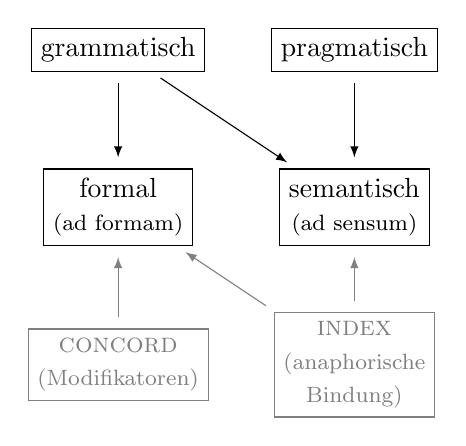
\begin{tikzpicture}[baseline=(grm.base), shorten >= 4pt, shorten <= 4pt]
	\node [draw, rectangle, align=center] (frm) at (0,0) {
		formal\\ \footnotesize (\fw{ad formam})
	};
	\node [draw,rectangle, align=center] (sem) at (3,0) {
		semantisch\\ \footnotesize (\fw{ad sensum})
	};
	\node [draw, rectangle] (grm) at (0,2) {grammatisch};
	\node [draw, rectangle] (prg) at (3,2) {pragmatisch};
	\draw [-latex] (grm) -- (frm);
	\draw [-latex] (grm) -- (sem);
	\draw [-latex] (prg) -- (sem);

	\node [draw, rectangle, align=center, gray] (con) at (0,-2) {
		\textsc{concord} \\
		\footnotesize (Modifikatoren)
	};
	\node [draw, rectangle, align=center, gray] (idx) at (3,-2) {
		\textsc{index} \\
		\footnotesize (anaphorische\\
		\footnotesize Bindung)
	};
	\draw [-latex, gray] (con) -- (frm);
	\draw [-latex, gray] (idx) -- (frm);
	\draw [-latex, gray] (idx) -- (sem);
\end{tikzpicture}
\caption%
	[Einteilung der Kongruenztypen und beteiligte Merkmale nach Wechsler~\&~%
	Zlatić]%
	{Einteilung der Kongruenztypen und beteiligte Merkmale nach
	\citet{wechslerzlatic2003}}
\label{fig:termini}
\end{figure}

Ein weiterer wichtiger Faktor in der Chrakterisierung von Kongruenzbeziehungen
nach \citet{corbett2006} ist die Domäne. Dieser Begriff wird von
\citet{corbett2006} nicht formal definiert. Aus seinen Ausführungen ist aber zu
entnehmen, dass damit der Abstand zwischen Controller und Target im Sinne der
Konstituenz von Sätzen gemeint ist. So gibt es nach \citet[54]{corbett2006}
vier Domänen mit wachsender Lokalität und abnehmender Kanonizität:

\begin{enumerate}[noitemsep]
	\item innerhalb der NP;
	\item außerhalb der NP aber innerhalb des Teilsatzes;
	\item außerhalb des Teilsatzes aber innerhalb des Satzes;
	\item außerhalb des Satzes.
\end{enumerate}

In \crefrange{ex:beidedomains_1}{ex:beidedomains_4} wird jeweils ein Beispiel
pro Domäne gegeben. In \cref{ex:beidedomains_1} stellt \lit{bede} `beide' als
Target einen Modifikator seines Controllers \lit{wingarten} `Weingarten' in
derselben NP beziehungsweise in derselben Nominalgruppe dar. Das Target steht
attributiv zum Controller.

\begin{exe}
\ex \label{ex:beidedomains_1}
	\gll die bede wingarten \\
		die beide-\textsc{acc.pl.m.st} Weingarten-\textsc{acc.pl.m} \\
	\trans `die beiden Weingärten'
		\parencites%
			(Nr.~1221, Zürich, 1290)%
			[484:9]{cao2}
\end{exe}

Der Controller \lit{zil} `Ziele, Fristen' in \cref{ex:beidedomains_2} bildet
den Kopf der in sich abgeschlossenen Genitiv-NP \lit{der vor genanten zil} `der
vorgenannten Ziele'. \textins{\lit{B}}\lit{eidiv} `beide' als darauf bezogenes
Target steht außerhalb davon als Kopf der darüber liegenden NP, aber dennoch im
gleichen Satzteil wie \lit{zil} `Ziele, Fristen', da die komplexe NP
\lit{der vor genanten zil / ainez / oder beidiv} `eines oder beide der
vorgenannten Ziele' das Akkusativobjekt zu \lit{verſitzzet} `versäumt'
ist. Das Target steht in einer anaphorischen Beziehung zum Controller.

\begin{exe}
\ex \label{ex:beidedomains_2}
	\gll ſwenne man der {vor genanten} zil / ainez / oder
		beidiv \textelp{} verſitzzet \\
		so=wenn man der vorgenannten Ziel[\textsc{gen.pl.n}] {} eines {}
		oder beide-\textsc{acc.pl.n.st} {} versäumt \\
	\trans `falls man eines oder beide der vorgenannten Ziele \textelp{}
		versäumt'
		\parencites%
			(Nr.~619, Augsburg, 1283)%
			[47:31]{cao2}
\end{exe}

In \cref{ex:beidedomains_3} ist das Target \lit{beideu} `beide' auf den
Controller \lit{rihtær} `Richter' bezogen, befindet sich formal aber nicht im
gleichen Satzteil wie dieser, dennoch aber im gleichen (Teil-)Satz, insofern
beide NPs vom gleichen Verb \lit{ſprachen} `sprachen' abhängen. Auch hier ist
die Kongruenzbeziehung anaphorisch.

\begin{exe}
\ex \label{ex:beidedomains_3}
	\gll Die rihtær ſprachen beideu {dar zuͦ} \\
		die Richter[\textsc{nom.pl.m}] sprachen beide-\textsc{nom.pl.n.st}
			dazu \\
	\trans `die Richter äußerten sich beide dazu'
		(%
			B1: 28ra:8;
			\cite[vgl.][267 {[=~V.~10090]}]{schroeder1895}%
		)
\end{exe}

Im letzten Schritt bezieht sich das Target \lit{bede} `beide' in
\cref{ex:beidedomains_4} zwar auf \lit{herren} `Herren', doch bildet
\lit{herren} das Subjekt zum Verb \lit{lident} `leiden', während
\lit{bede} zusammen mit dem Personalpronomen \lit{Si} `sie' das
Subjekt von \lit{ligent} `liegen' bildet. Damit stehen der (Erst-)Controller
\lit{herren} und das Target \lit{bede} in unterschiedlichen Sätzen. Das
\norm{bėide}-Target bezieht sich ebenfalls anaphorisch auf seinen Controller.

\begin{exe}
	\ex \label{ex:beidedomains_4}
		\gll Min herren lident ovch groze not. \\
			mein Herr-\textsc{nom.pl.m} leiden auch große Not \\
	\sn \gll Si ligent bede fvͤr tot \\
			\textsc{3pl\subM.nom} liegen beide-\textsc{nom.pl.m.st} für tot \\
	\trans `Meine Herren leiden auch große Not. Sie liegen beide tot
		\textins{darnieder}.'
		(%
			VB: 86ra:3--4;
			\cite[vgl.][301 {[=~V.~12033--12034]}]{schroeder1895}%
		)		
\end{exe}

\section{Index und Concord}
\label{sec:indexconcord}

\phantomsection
\label{phsec:index}
Das Merkmal \textsc{index} ist in der HPSG seinerseits Teil des Merkmals
\textsc{content} eines lexikalischen Zeichens, das sich aus der Semantik
speisende Informationen über dessen Denotat enthält, konkret also
grammatikalisierte Personenmerkmale wie \textsc{person}, \textsc{numerus} und
\textsc{genus} \citep[15--17]{wechslerzlatic2003}. Auch in der mit der HPSG
verwandten \fw{Lexical-Functional Grammar} (LFG;
\cites{kaplanbresnan1982}{bresnan2001}{bresnanetal2016}) existiert ein solches
Merkmal \citep[189--190]{bresnanetal2016}. Das \textsc{index}-Merkmal bildet
die Basis für anaphorische Referenz, indem es ein Individuum oder ein Ding als
Instanz des Bezeichneten im Diskurs verankert
\citep[10--11]{wechslerzlatic2003}. Während eine große Nähe zwischen
\textsc{index} und Semantik konstatiert wird, ist diese nicht absolut, da auch
das generische Pronomen \fw{man} oder das expletive Subjektspronomen \fw{es}
einen \textsc{index} besitzen, obwohl sie sich nicht auf eine bestimmte
semantische Größe beziehen \citep[11--13]{wechslerzlatic2003}. Dies wird bei
der Konjugation von Verben und der Bindung von Reflexivpronomen sichtbar
\cref{ex:explvbkonj}.

\begin{exe}
\ex \label{ex:explvbkonj}
	\begin{xlist}
	\ex Es$_i$ regnet$_i$.
	\ex Man$_i$ kann$_i$ es sich$_i$ vorstellen.
	\end{xlist}
\end{exe}

\citet{kingdalrymple2004} argumentieren des Weiteren, dass \textsc{index} in
koordinierten nominalen Strukturen ein nicht-distributives Merkmal darstellt,
indem die Kombination zweier Substantive einen neuen Index erhält, mit dem
kongruiert wird \citep[74--76]{kingdalrymple2004}. \fw{Jan} und \fw{Markus} in
\cref{ex:coordidx} haben zwar jeder für sich einen Singular-\textsc{index}, die
Gruppe \fw{Jan und Markus} hat aber einen Plural-\textsc{index}, was sich in
der Kongruenz zwischen Subjekt und Verb zeigt.

\begin{exe}
\ex\label{ex:coordidx}
\begin{xlist}
	\ex[]{[Jan$_i$ und Markus$_j$]$_k$ spielen$_k$ Fußball.}
	\ex[*]{Jan$_i$ und Markus$_j$ spielt$_{i/j}$ Fußball.}
\end{xlist}
\end{exe}

\phantomsection
\label{phsec:concord}
Das Gegenstück zum \textsc{index} bildet \textsc{condord}, das in der HPSG Teil
des Kopfmerkmals ist \citep[17]{wechslerzlatic2003}. Das Merkmal
\textsc{concord} existiert ebenso in der LFG \citep[189--192]{bresnanetal2016}
und enthält in beiden Theoriesystemen syntaktisch relevante Informationen über
den nominalen Phrasenkopf, die im Deutschen für einzelne, unkoordinierte NPs
weitgehend deckungsgleich mit denen des \textsc{index} sind:%
%
	\footnote{\citet{wechslerzlatic2003} untersuchen den Fall des
	Bosnisch-Kroatisch-Mazedonisch-Serbischen (BKMS), in dem es Substantive
	gibt, für die dies nicht der Fall ist.}
%
Zu den Merkmalen \textsc{numerus} und \textsc{genus} tritt das strukturelle
Merkmal \textsc{kasus}, dafür spielt \textsc{person} hier keine Rolle.
Kongruenz über das Merkmal \textsc{concord} herrscht typischerweise zwischen
einem nominalen Kopf und seinen Modifizierern, was in der HPSG mit dem
\fw{Head Feature Principle} begründet wird. Dieses besagt im Grunde, dass ein
Phrasenkopf seine grammatischen Informationen mit seinen Töchtern teilt
\autocite[vgl.][22]{wechslerzlatic2003}. Daher ist im Gegensatz zu
\textsc{index} das Merkmal \textsc{concord} lokal auf die NP beschränkt,
während das \textsc{index}-Merkmal überall dort vorkommt, wo anaphorische
Bindung eine Rolle spielt
\parencites[14--16, 22]{wechslerzlatic2003}[189]{bresnanetal2016}.

In Bezug auf koordinierte Substantive wie in \cref{ex:coordidx} sei angemerkt,
dass \citet[76--78]{kingdalrymple2004} \textsc{concord} im Gegensatz zu
\textsc{index} als distributives Merkmal analysieren. Dies bedeutet, dass
Modifizierer von koordinierten Substantiven mit jedem Konjunkt einzeln in
\textsc{condord}-Merkmalen übereinstimmen müssen, um einen akzeptablen Ausdruck
zu produzieren. Das Beispiel in \cref{ex:engartdiscong} illustriert dies,
insofern \fw{these} `diese' nur dann verwendet werden kann, wenn beide von ihm
determinierten Konjunkte jeweils im Plural stehen \cref{ex:engartdiscong_1}
oder wenn es lediglich ein einzelnes Substantiv determiniert und stattdessen
die Konjunktion auf höherer syntaktischer Ebene stattfindet
\cref{ex:engartdiscong_4}.

\begin{exe}
\ex\label{ex:engartdiscong}
	Englisch \parencite[nach][70]{kingdalrymple2004}
	\begin{xlist}
	\ex[]{these[\textsc{pl}] boys[\textsc{pl}]
		and girls[\textsc{pl}]}
		\label{ex:engartdiscong_1}
	\ex[*]{these[\textsc{pl}] boys[\textsc{pl}]
		and girl[\textsc{sg}]}
		\label{ex:engartdiscong_2}
	\ex[*]{this[\textsc{sg}] boy[\textsc{sg}]
		and girls[\textsc{pl}]}
		\label{ex:engartdiscong_3}
	\ex[]{these[\textsc{pl}] boys[\textsc{pl}]
		and this[\textsc{sg}] girl[\textsc{sg}]}
		\label{ex:engartdiscong_4}
	\end{xlist}
\end{exe}

\section{Genus, Sexus und Belebtheit}
\label{sec:gendsex}

Wenn im Folgenden von \textit{Genus} die Rede ist, bezeichnet der Begriff das
grammatische Geschlecht eines Substantivs. Da es sich beim Mittelhochdeutschen
um eine flektierende Sprache handelt, ist die häufig zitierte Definition von
\citet[231]{hockett1958} relevant, die Genera relational begreift als Klassen
von Substantiven, die sich im Verhalten von darauf bezogenen Wörtern zeigen.%
%
	\footnote{\foreigntextcquote{english}[231]{hockett1958}{Genders are classes
		of nouns reflected in the behavior of associated words}.}
%
Genus wird also als grammatische Kategorie der Klassifizierung von Substantiven
aufgefasst, die an der Kongruenzform von darauf bezogenen Targets erkennbar
ist. Im Sinne \posscite[62--63]{corbett1991} bezieht sich diese Definition auf
\fw{covert gender}, bei dem die Klassenzugehörigkeit eines Substantivs nicht
aus seiner Form erschlossen werden kann. Wie zum Beispiel von
\citet{koepckezubin2017} gezeigt, besitzt das Deutsche allerdings durchaus
Aspekte overter Genuszuweisung, sei es durch die Semantik des Bezeichneten, die
Zugehörigkeit zu einer bestimmten Klasse von Dingen oder die phonologische
Struktur des Lexems.

Von den 257 von \citet{corbett2013b} untersuchten, typologisch diversen
Sprachen besitzen 84 (32,7\,\%) ein sexusbasiertes System als semantische
Grundlage der Klasseneinteilung; in den Daten von \tit{Grambank}
\autocite{skirgardetal2023} fällt dieser Wert auf lediglich 410 von 2.206
Varietäten (18,6\,\%; \cite[siehe][]{haynie:gb051}). Gerade der Aspekt der
Sexusbasiertheit führt zu einiger Komplexität beim Zusammenspiel von Geschlecht
im biologischen und soziokulturellen Sinn sowie der sekundären Nutzung von
Geschlecht als grammatischer Kategorie \autocites[dazu
ausführlich][]{kotthoffnuebling2018}{steriopolosteriopolo2022}. Die
Doppeldeutigkeit von \fw{gender} im Englischen als Bezeichnung einerseits für
das soziale Geschlecht und die damit verbundene Geschlechter\-rollen\-praxis
und andererseits für die grammatische Kategorie verkompliziert tendenziell den
Diskurs, indem zwei miteinander interagierende Ebenen terminologisch vermischt
werden.

Der Zusammenhang von sozialem Geschlecht und Sprache führt immer wieder zu
stark emotional geführten, sprachästhetisch bis sozialkritisch motivierten
Debatten insbesondere über die Notwendigkeit der expliziten sprachlichen
Sichtbarmachung von Frauen durch Movierung der maskulinen Form eines Nomen
Agentis sowie von Personen, die sich dem nicht-cis-nicht-heterosexuellen
Spektrum zugehörig fühlen, durch weitere typografische Mittel \autocite[dazu
kritisch resümierend][]{kasper2022}. Mit \citet[61--89]{kotthoffnuebling2018}
ist anzumerken, dass der Laiendiskurs um das sogenannte \q{Gendern} häufig
sehr oberflächlich bleibt. Ein explizit andro\-zentrischer Bias durchdringt die
gesamte Nominalmorphologie des Deutschen sehr viel tiefer.

Aus sprachhistorischer Sicht gründet sich diese kritische Beobachtung letztlich
darin, dass das Urindogermanische vor der Abspaltung des anatolischen Zweigs
wahrscheinlich lediglich eine Distinktion \textsc{[±\,belebt]} oder
\textsc{[±\,human]} besaß, die sowohl im Zusammenhang mit
Individualisierbarkeit als auch in syntaktischer Hinsicht mit Agensfähigkeit
stand. Das spätere Maskulinum setzt das belebte Genus fort, das Neutrum das
unbelebte. Zur expliziten Kennzeichnung von belebten Feminina hat sich sekundär
das Suffix \fw{*-h₂} etabliert, das darüber hinaus zur Derivation von
Kollektiva und Abstrakta diente, wie in \cref{tab:pie_h2} gezeigt
\autocites%
	[73--74, 77]{ringe2017}%
	[195--197, 205--207]{fritzmeierbruegger2021}%
	[167--172]{klein2022}%
. Mit \citet[313]{corbett1991} ist anzumerken, dass die Umnutzung und
Rekombination von vorhandenem morphologischen Material bei der
Ausdifferenzierung von Genera keine Seltenheit darstellt.

\begin{table}
\centering
\caption{\fw{*h₂}-Derivate im Urindogermanischen}
\begin{tabular}[t]{
	l @{} l @{} l @{~} l
	c
	l @{} l @{} l @{~} l
	l
}

\toprule

\fw{*wĺ̥kʷ}
	& \fw{-o}
	& \fw{-s}
	& `Wolf'
& $\to$
& \fw{*wl̥kʷ}
	& \fw{-í}
	& \fw{-h₂}
	& `Wölfin'
& \parencite[102, 132]{ringe2017} % Kap. 3.2.2.i, 3.2.4.iii
\\

\fw{*kʷékʷl}
	& \fw{-o}
	& \fw{-s}
	& `Rad'
& $\to$
& \fw{*kʷekʷl}
	& \fw{-é}
	& \fw{-h₂}
	& `Rädersatz'
& \parencite[59]{ringe2017} % Kap. 2.3.4.ii
\\

\fw{*bʰewg-}
	& %
	& %
	& `fliehen'
& $\to$
& \fw{*bʰug}
	& \fw{-á}
	& \fw{-h₂}
	& `Flucht'
& \parencite[74]{ringe2017} % Kap. 2.4.2.i
\\

\bottomrule
\end{tabular}
\label{tab:pie_h2}
\end{table}

Bezüglich der eingangs referierten Definition von Genus als relationaler Größe
hebt \citet[42]{koepcke1982} hervor, dass \blockquote{\textins*{d}er
kommunikative Wert von Genuszuweisungen \textelp{} in erster Linie darin
\textins{liegt}, daß sie dem Sprachbenutzer im kommunikativen Zusammenhang
anaphorische Referenzierungen erleichtern}, zum Beispiel, indem häufig im
gleichen Kontext genannte Dinge unterschiedliche Genera besitzen \autocite[dazu
auch][320--323]{corbett1991}. Darüber hinaus vermag Genus auf der Ebene der
Pragmatik die Einstellung einer Sprecherin oder eines Sprechers zu
signalisieren, was Respekt oder Verachtung, Zu- oder Abneigung gegenüber einer
Person durch die Verwendung des \q{richtigen} oder \q{falschen} Genus in
Bezug auf deren Identität betrifft \autocite[322--323]{corbett1991}.

\citet{steriopolosteriopolo2022} verorten diese affektive Funktion des
Genus\-gebrauchs im sozialen Geschlecht (\fw{social gender}) als Bindeglied
zwischen biologischem und grammatischem Geschlecht. Sie attestieren dieser
Ebene, die den sozialen oder ontologischen Status eines Individuums anspricht,
eine starke emotionale Komponente, wenn durch abweichenden Genus\-gebrauch zum
Beispiel despektiertlich kommuniziert wird, dass sich eine Person nicht in
Einklang mit der ihr zugemessenen Geschlechterrolle verhält.
Abgesehen von lexikalisierten Fällen von abweichendem Genus wie
mittelhochdeutsch \norm{wīp} `Frau' (Neutrum mit Bezug auf eine weibliche
Person) oder \norm{kindelīn} `Kindlein' (Neutrum mit Bezug auf junge
Menschen), spielt situativ abweichender Genusgebrauch bei Personen im
Belegmaterial keine Rolle.

Im Zusammenhang mit \norm{bėide} `beide' kommen im Belegmaterial natürlich
nicht nur Personen vor, sondern häufig auch Sachen, wie etwa ein \norm{garte}
`Garten' und ein \norm{acker} `Acker', deren Verkauf die Urkunde Nr.~3249
\autocites(Freiburg i.\,Br., 1299)[][]{cao4} behandelt. Belebtheit macht sich
nicht nur bei der Genuszuweisung, sondern auch unter morphologischen
Gesichtspunkten bemerkbar, obwohl sie keine eigentliche grammatische Kategorie
des Mittelhochdeutschen darstellt. In den Worten \posscite[99]{dahl1999} ist
Belebtheit, also der Unterschied zwischen belebten und unbelebten Entitäten, in
den Grammatiken menschlicher Sprachen so allgegenwärtig, dass sie tendenziell
als selbstverständlich hingenommen und damit unsichtbar wird.%
%
	\footnote{\foreigntextcquote{english}[99]{dahl1999}{Animacy, or the
		distinction between animate and inanimate entities, is so pervasive in
		the grammars of human languages that it tends to be taken for granted
		and become invisible}.}

\begin{figure}
\centering
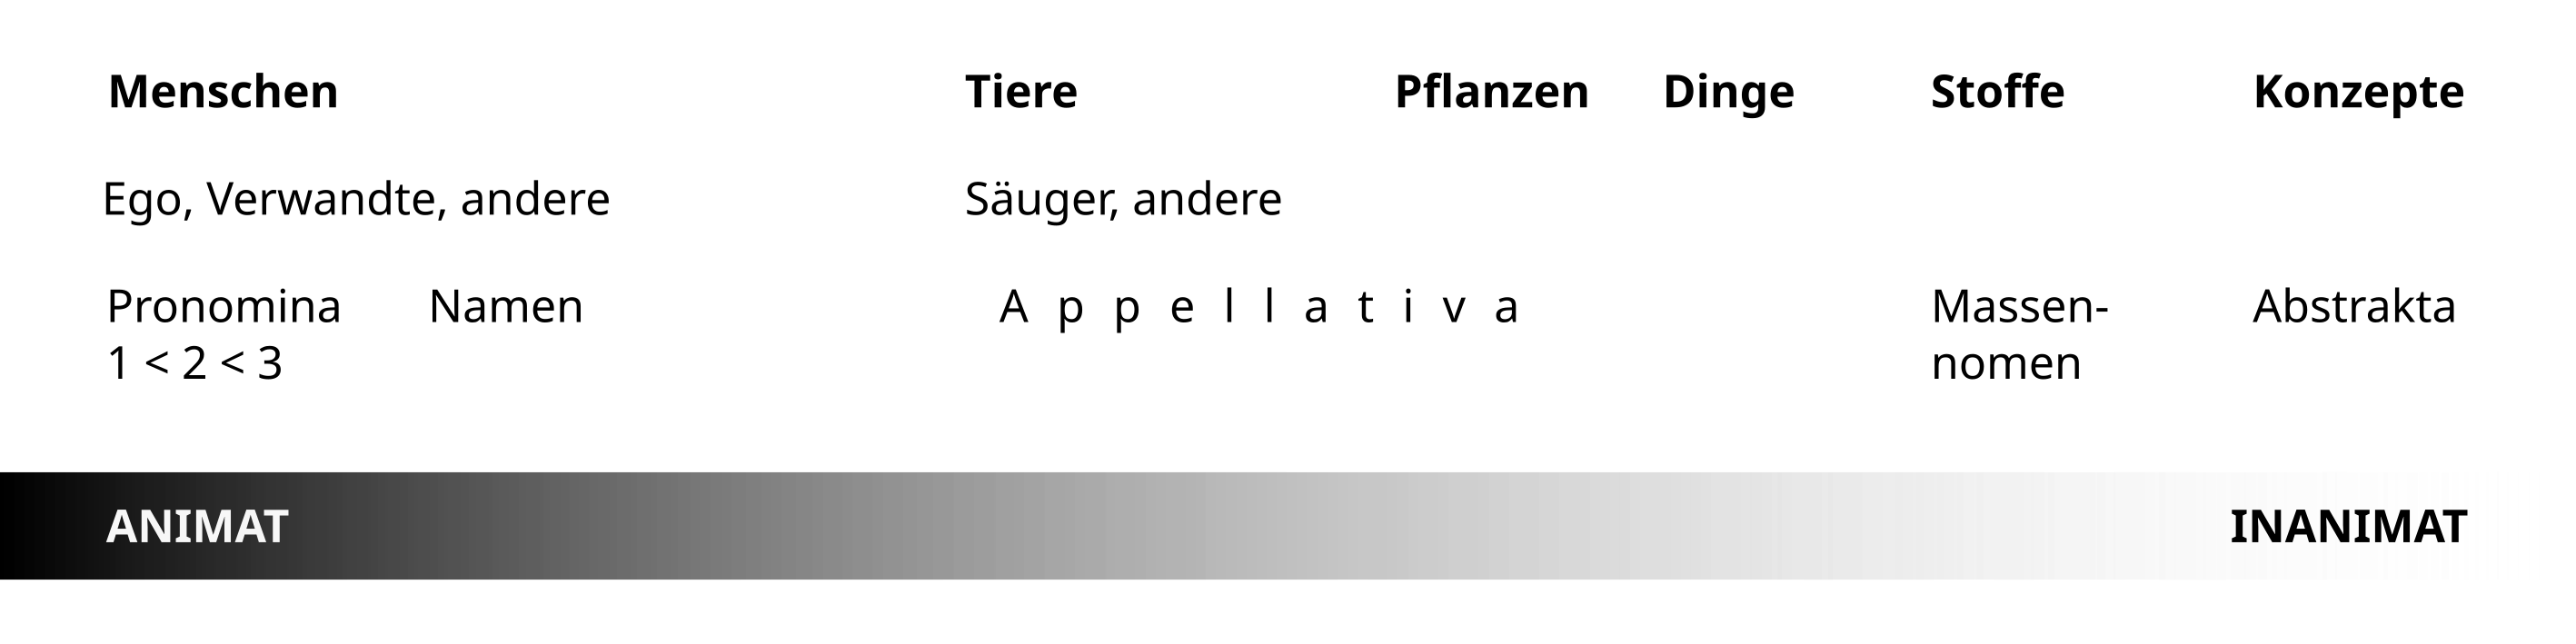
\includegraphics[
	width=\linewidth,
	keepaspectratio,
]{./figures/belebtheitshierarchie.png}
\caption{Belebheitshierarchie nach \citet[72]{kotthoffnuebling2018}}
\label{fig:animhier}
\end{figure}

Belebtheit wird als Kontinuum konzipiert; die Belebtheitshierarchie reicht von
Menschen als belebtester Kategorie über Tiere zu Gegenständen und Abstrakta als
am wenigsten belebt (siehe \cref{fig:animhier}). Die Sprecherinstanz steht
dabei gewöhnlich an der Spitze der Skala, da sie den Lokus der Wahrnehmung
bildet \autocites%
	{silverstein1976}%
	[185--200]{comrie1989}%
	[203]{bossong1998}%
	[40--46]{siewierska2004}%
	[439--441]{bickel2011}%
	[63--79]{kotthoffnuebling2018}. %
Belebtheit ist \citet[101--102, 110--112]{dahl1999} zufolge auch ein wichtiger
Faktor bei der Genuszuweisung, da ein hoher Grad von Belebtheit mit
semantischen Eigenschaften des Bezeichneten -- und hier gerade Sexus
beziehungsweise sexuelle Differenzierbarkeit -- als Quelle von Genus
korrelliert (\fw{referential gender}), während ein hoher Grad von Unbelebtheit
mit formalen Kriterien der Genuszuweisung einhergeht (\fw{lexical gender}). Wie
aus \cref{fig:animhier} deutlich wird, gibt es der Natur von Kontinua
entsprechend keine scharfe Grenze zwischen den Polen
\textsc{[+\,belebt]} und \textsc{[-\,belebt]}, sondern viele
Übergangs- und Zweifelsfälle.

Da die Personen, die in den hier untersuchten Texten benannt werden, seit
Jahrhunderten tot und im Fall der \KC{} zusätzlich literarisch
überformt sind, lässt sich nicht nachvollziehen, wie sich das Verhältnis von
sozialem und biologischem Geschlecht in jedem einzelnen Fall genau verhält,
zumal es anachronistisch wäre, moderne Konzepte von sexueller Identität auf das
Hochmittelalter beziehungsweise die Antike im Spiegel eines
hochmittelalterlichen Texts zu übertragen \autocite[siehe
z.\,B.][]{klinger2002}. Weil Kontexte, in denen cis- und heterosexuelle Normen
explizit unterlaufen oder infrage gestellt werden, im Belegmaterial nicht
vorkommen, gehe ich bei der Klassifizierung meiner Daten von cis- und
heteronormativen Gegebenheiten aus.

Wenn im Weiteren vereinfachend von \textit{Sexus} als semantischer Basis von
Genus die Rede ist, bezieht sich der Begriff nicht primär auf eine biologische
Lesart. Vielmehr ist damit diejenige Geschlechter\-rolle gemeint, die in der
Wortbedeutung einer Personenbezeichnung angelegt ist und daher stereotyp
erwartet wird oder die vom Textzusammenhang etwa durch Namennennung implizierte
Geschlechterrolle. Gerade in der älteren Literatur ist in diesem Kontext häufig
vom \q{natürlichen Geschlecht} die Rede; \citet[67]{panther2009} spricht
diesbezüglich vom \q{konzeptuellen Genus}. Um auf das zuvor zitierte Beispiel
zurückzukommen, wird im Folgenden die Bezeichnung \fw{Mutter} entsprechend der
in der Wortbedeutung angelegten weiblichen Geschlechterrolle als eine weibliche
Person denotierend aufgefasst
\autocite[vgl.][s.\,v.~\fw{Mutter}]{duden-online}.

Bezüglich komplexer Kombinationen von Genus, Sexus und der Kongruenz darauf
bezogener Targets diskutiert \textcite[183--184]{corbett1991} sogenannte
\fw{Lexical Hybrids}, also Substantive, deren Genus und Sexus nicht
übereinstimmen und bei denen in der pronominalen Referenz typischerweise
Variation zwischen formaler und semantischer Kongruenz herrscht, also zum
Beispiel, wenn \fw{das Mädchen} im weiteren Verlauf formal mit \fw{es} oder
semantisch mit \fw{sie} pronominal referenziert wird. \citet{klein2022}
unterscheidet darüber hinaus zwischen Lexical Hybrids im engeren Sinn und
Epikoina.

Bei Lexical Hybrids im engeren Sinn liegt ein Konflikt zwischen Genus und Sexus
auf der lexikalischen Ebene vor \autocite[145]{klein2022}. In diesem
Zusammenhang ist das historisch langlebige Wort für `Frau' als formales
Neutrum mit weiblicher Denotation hervorzuheben: Im Alt- und
Mittelhochdeutschen lautet es \norm{wīb} beziehungsweise \norm{wīp}. Auch im
modernen Deutschen findet sich \fw{Weib} noch mindestens bis ins
20.~Jahrhundert in nicht-pejorativer Verwendung \autocite[166]{fleischer2012}.
Im Fall von \fw{Mädchen} wird konventionell eine junge weibliche Person
bezeichnet, das neutrale Genus wird dem Lexem durch das Diminutivsuffix
\norm{-chen} formal zugewiesen. Auch bei Bezeichnungen wie \fw{die Wache} oder,
pejorativ, \fw{die Type} und \fw{die Tunte}, kommt es zu Diskrepanzen in der
Lexik, weil diese formal zu den Feminina zählen, jedoch in ihrer Semantik
gewöhnlich mit Männern assoziiert werden
\autocite[vgl.~auch][67--68]{panther2009}.

Eine andere Spielart von Lexical Hybrids liegt bei Epikoina vor, also im Grunde
sexus\-indifferenten Lexemen wie \fw{Person}, das zwar formal feminin ist, sich
aber der Wortbedeutung nach sowohl auf Männer als auch Frauen beziehen kann,
oder \fw{Mensch}, das zwar formal maskulin ist, sich aber ebenfalls auf
Menschen jeglichen Geschlechts bezieht.%
%
	\footnote{Siehe aber die Ergebnisse der Fragebogenstudie zu
		\fw{Mensch} und \fw{Person} von \citet[174--183]{klein2022}, bei denen
		die Probandinnen und Probanden in Einklang mit dem Genus des jeweiligen
		Lexems \norm{Mensch} eher mit Männern und \fw{Person} eher mit Frauen
		assoziiert haben.}
%
In diesen Fällen liegt in grammatisch spezifischen Kontexten ein Konflikt auf
der referenziellen Ebene vor, weil das jeweils geltende Sexusmerkmal von der
bezeichneten Person abhängt und damit vom konkreten Gebrauchskontext bestimmt
wird \autocite[142--144]{klein2022}.

Ein im Deutschen langlebiges Epikoinon ist \fw{Kind}, althochdeutsch
\norm{kind} und mittelhochdeutsch \norm{kint}, das zwar formal neutral ist,
sich im konkreten Fall aber sowohl auf Mädchen als auch auf Jungen beziehen
kann, genereller auf nicht-erwachsene Menschen.%
%
	\footnote{Darüber hinaus kann sich \fw{Kind} im übertragenen Sinn auch auf
		erwachsene Menschen beziehen, zum Beispiel, wenn damit die
		Abhängigkeitsbeziehung zu den Eltern oder metaphorisch zu Gott betont
		wird \autocite[s.\,v.~\textit{kint}]{lexer:mhdhwb}. In manchen Fällen
		kann \fw{Kind} auch besonders auf Mädchen oder junge Frauen bezogen
		sein
		\autocites[s.\,v.~\textit{kint}]{drw}[s.\,v.~\textit{Kind}]{duden-online}.}
%
Insbesondere \fw{Kind} verdient Aufmerksamkeit, da die Variation zwischen
Neutrum in Einklang mit dem formalen Genusmerkmal sowie Maskulinum oder
Femininum in Übereinstimmung mit dem semantischen Sexusmerkmal der bezeichneten
Person auch von deren Alter abhängt, insofern Kinder häufig als weniger agentiv
und damit weniger belebt als Erwachsene konzeptualisiert werden
\autocites[196]{comrie1989}[258--259]{birkenesfleischer2022}[151]{klein2022}.

In dieser Hinsicht stellt \citet[172--174]{klein2022} eine Hierarchie innerhalb
der Epikoina auf, da Abstufungen in der Belebtheit und, damit einhergehend, der
von Menschen wahrgenommenen Ausgeprägtheit sexueller Unterschiede zwischen
Individuen der bezeichneten Gruppe einen Einfluss darauf haben, ob ein
Epikoinon beim pronominalen Bezug eher mit formaler oder semantischer Kongruenz
steht \autocite[vgl.~auch][74--83]{kotthoffnuebling2018}. Sogenannte generische
Maskulina, also (vermeintlich) geschlechtsneutrale Bezeichnungen wie
\fw{Bürger} und \fw{Gast}, mittelhochdeutsch \norm{burgǟre} und \norm{gast},
bewegen sich darüber hinaus im Spannungsfeld zwischen einer spezifischen,
referenziellen Lesart mit Bezug auf einen bestimmten Mann einerseits und einer
unspezifischen, nicht-referenziellen Lesart mit Bezug auf irgendein Individuum
aus der benannten Gruppe und die damit assoziierten stereotypen
Geschlechterrollen andererseits
\autocites[91--122]{kotthoffnuebling2018}[159--160, 179--180]{klein2022}. Wo
zum Beispiel \norm{burgǟre} anders als in \cref{ex:nongenmasc} keine
spezifische Referenz besitzt, gehe ich im Folgenden vereinfachend davon aus,
dass damit allgemein die Stadt bewohnende Menschen gemeint sind.

\begin{exe}
\ex \label{ex:nongenmasc}
	\gll Hermann der Marſpurrer \textelp{} vnd Cvͦnrat der Turſte
			\textelp{} die {vor genemten} burgare bede von V́berlingen \\
		Hermann[\textsc{nom.sg.m}] der Marspurrer {} und
			Konrad[\textsc{nom.sg.m}] der Turste {} die vorgenannten
			Bürger[\textsc{nom.pl.m}] beid-\textsc{nom.pl.m} von Überlingen \\
	\trans `Hermann der Marspurrer \textelp{} und Konrad der Turste
		\textelp{}, die vorgenannten beiden Bürger von Überlingen' \\
		\parencites%
			(Nr.~N~288, Überlingen, Bodenseekr., 1285)%
			[223:19--21]{cao5}
\end{exe}

Körperteile stellen eine weitere Übergangskategorie dar, indem sie
Dingcharakter haben, aber Teil eines Organismus sind. Im speziellen Kontext mit
\norm{bėide} `beide' liegen in der Belegsammlung zu dieser Arbeit keine
Fälle von kombiniertem pronominalen Bezug auf Körperteile vor, sondern
lediglich der Fall in \cref{ex:bodyparts_attr}, bei dem \lit{baide}
`beide' attributiv \lit{hênde} `Hände' quantifiziert, sowie mehrere
Fälle mit \norm{bėide} als Konjunktion, von denen einer exemplarisch in
\cref{ex:bodyparts_conj} zitiert wird. In diesem Beispiel wird die Koordination
von \lit{ader} `Ader' und \lit{lit} `Glied' mit \lit{baidiv}
`beide' eingeführt, jedoch im weiteren Verlauf kein kombinierter Bezug auf
beide Konjunkte durch Pronomina hergestellt.

\begin{exe}
\ex \begin{xlist}
	\ex \label{ex:bodyparts_attr}
		\gll Si wand ír baide hênde \\
			sie wand ihr beid-\textsc{acc.pl.f.st} Hand-\textsc{acc.pl.f} \\
		\trans `Sie wand ihre beiden Hände.'
			(%
				K:~6rb:19, vgl. abweichend
				A1:~4va:26--27,
				% H:~5va:4,
				% M:~7vb:8,
				B1:~4vb:49,
				% P:~9ra:5;
				\cite[98 {[=~V.~913]}]{schroeder1895}% setno 1065
			)

	\ex \label{ex:bodyparts_conj}
		\gll baidiv ader unt lit. \\
			beide Ader[\textsc{acc.sg.f}] und Glied[\textsc{acc.sg.m/n}] \\
		\trans `sowohl Ader als auch Glied'
			(%
				A1:~32rb:31, vgl.
				% H:~44va:15,
				% M:~56vb:21,
				C1:~39rb:3,
				% K:~45ra:32,
				% Z:~147va:20;
				\cite[218 {[=~V.~7468]}]{schroeder1895}% setno 2018
			)
\end{xlist}
\end{exe}

Der Belebtheitsstatus von Körperteilen ist zumindest im modernen
Standarddeutschen beachtenswert, da sich deren Possessivsyntax von anderen,
weniger belebten Dingen abhebt, wie die Beispiele in \cref{ex:stdgeralien}
zeigen. Dieses Verhalten lässt sich als Unterschied in der Alienabilität fassen
\autocites{nichols1988}[17--18]{heine1997}. Eine kursorische Suche im \REM{}
nach dem inalienablen Typ mit \textsc{pronomen}~(\textsc{dat}) --
\textsc{artikel}~(\textsc{acc}) -- \textsc{substantiv} hat keine Ergebnisse
geliefert.

	\begin{exe}
	\ex \begin{xlist}
		\ex[]{Ich wasche mein Auto.
				\jambox{\hphantom{*\,}$\textsc{[+ alienabel]}$}}
		\ex[]{Ich wasche mir die Hände.
				\jambox{\hphantom{*\,}$\textsc{[- alienabel]}$}}
		\ex[*]{Ich wasche mir das Auto.
				\jambox{*\,$\textsc{[- alienabel]}$}}
		\end{xlist}
		\label{ex:stdgeralien}
	\end{exe}

Neben formalen und semantischen Merkmalen kann auch die Distanz zwischen einem
Controller und seinem Target einen Einfluss auf die Wahl der Kongruenzform
haben, wenn mehrere Möglichkeiten bestehen. Unter dieser Prämisse untersuchen
\citet{panther2009} und \citet{binanzeretal2022} semantische Kongruenz für die
moderne Standardsprache des Deutschen, \citet{fleischer2012} geht diesem Aspekt
in diachroner Perspektive nach. Diesen Studien ist die Erkenntnis gemein, dass
Kongruenz \fw{ad sensum} zum einen mit wachsender linearer Distanz zwischen
Controller und Target tendenziell zunimmt, zum anderen verschiedene Arten von
Pronomina und anaphorischen Ausdrücken eine unterschiedlich hohe Affinität zur
semantischen Kongruenz aufweisen, sich also auch die syntaktische Domäne von
Controller und Target auf die Wahl der Kongruenzform auswirkt \autocites%
	(siehe auch \cref{sec:ctrltarg,sec:kongrhier})%
	[84--85]{panther2009}[197--199]{fleischer2012}%
.

Da insgesamt also damit zu rechnen ist, dass die Semantik und der pragmatische
Kontext einer Personenbezeichnung einen starken Einfluss auf die Genuskongruenz
von anaphorischen Targets haben, möchte ich im Folgenden sowohl formale als
auch semantische Geschlechtsmerkmale in der Annotation von Beispielen
konsequent abbilden. Zu diesem Zweck erweitere ich die herkömmliche Annotation
des Genus um einen Index, der den Sexus kodiert, wie in \cref{tab:gendsex}
angegeben.

\begin{table}[h]
\centering
\caption{Abkürzungen für grammatisches und semantisches Geschlecht}
\begin{tabular}{@{} l l l l @{}} % @{\hspace{4\tabcolsep}}
\toprule
\mc{2}{c}{Genus} & \mc{2}{c}{Sexus} \\ % \smallskip

\cmidrule(r){1-2}
\cmidrule(l){3-4}

\textsc{m} & maskulin & \SM & männlich     \\
\textsc{f} & feminin  & \SF & weiblich     \\
\textsc{n} & neutral  & \SI & unbelebt     \\
           &          & \SA & unspezifisch \\
           &          & \SX & unbekannt    \\
\bottomrule
\end{tabular}
\label{tab:gendsex}
\end{table}

Dabei wird für die Bezeichnung der formalen Kategorie \textit{Genus} die
lateinische Terminologie verwendet, für die Bezeichnung der semantischen
Kategorie \textit{Sexus} die deutsche. Zum Beispiel wird
\norm{wīp} `Frau' als \NeutF\ annotiert, \norm{kint} `Kind' je
nachdem, ob das Geschlecht des Kindes im Kontext bekannt ist, als \NeutM,
\NeutF\ oder \NeutX. Wenn sich im Kontext eines Beispiels \norm{ėrbe}
`Erbe' oder \norm{burgǟre} `Bürger' nicht auf eine bestimmte Person beziehen
lassen, also unspezifische Referenz vorliegt, werden sie mit \MascA\ annotiert.
Im Fall von \norm{schuech} `Schuh' als unbelebtem Substantiv steht \MascI, bei
\norm{minne} `Liebe' als Abstraktum \FemI. Da es sich bei Körperteilen nicht um
Menschen handelt, wurden auch diese unter Vorbehalt als Inanimata gewertet. So
wird \norm{hant} `Hand' mit \FemI{} annotiert, es sei denn, damit ist
metonymisch ein Diener oder eine Dienerin gemeint, in welchem Fall die
Annotation entsprechend \FemM{} oder \FemF{} lautet. Semantisch komplexe
Bezeichnungen wie \norm{drīvaltichėit} `Dreifaltigkeit' kommen im ausgewerteten
Material nicht vor. \norm{Got} `Gott' wurde gemäß seiner Bezeichnung als
\norm{truhtīn} `Herrscher' und \norm{hērre} `Herr' \autocite[z.\,B.][234
{[=~V.~8314]}, 323 {[=~V.~13525]}]{schroeder1895} als \MascM\ gewertet.

Im modernen Standarddeutschen liegen darüber hinaus einzelne Wörter wie
\fw{Schild} oder \fw{Korpus} vor, die je nach Bedeutungskontext
unterschiedliche Genera besitzen: \fw{das Schild} (\NeutI) für die
Hinweistafel, \fw{der Schild} (\MascI) für den Schläge und Hiebe abwehrenden
Schirm; \fw{der Korpus} (\MascI) als Schallkörper eines Saiteninstruments,
\fw{das Korpus} (\NeutI) als strukturierte Sammlung von Texten oder
Belegstellen. Ferner ist neben standardsprachlichem \fw{die Butter} (\FemI)
regional auch \fw{der Butter} (\MascI) verbreitet
\autocite[s.\,v.~\textit{der/die Butter}]{elspassmoeller2003}. Ein
mittelhochdeutsches Beispiel für Substantive mit bedeutungs\-unterscheidendem
Genus ist \norm{dęr tėil} (\MascI) `Anteil, Zugeteiltes, Eigentum' gegenüber
\norm{daȥ tėil} (\NeutI) `Teil von einem Ganzen, Stück, Seite, Abteilung'
\autocite[s.\,v.~\textit{teil}]{lexer:mhdhwb}.

Des Weiteren liegt in der mittelhochdeutschen Periode noch eine größere Zahl an
Substantiven vor, deren Genus bei gleicher Bedeutung variabel belegt ist oder
die ihr Genus im Lauf der Zeit gewechselt haben \autocite[157--166]{ksw2}, zum
Beispiel \norm{die} (\FemI) oder \norm{daȥ jārƶīt} (\NeutI) `Jahrestag'
beziehungsweise mittel\-hoch\-deutsch \fw{die wiƶƶe} (\FemI) `Wissen, Verstand,
Klugheit' \autocite[vgl.][s.\,v.~\textit{witze}]{lexer:mhdhwb} gegenüber
neu\-hoch\-deutsch \fw{der Witz} (\MascI). In diesen Fällen wurde im Kontext
der jeweiligen Textstelle nach Hinweisen gesucht, mit welchem Genus das
jeweilige Lexem verwendet wird, soweit dies möglich war.

\section{Gender Resolution}
\label{sec:gendres}

Ein Problem für Kongruenz entsteht dann, wenn zum Beispiel durch Koordination
von zwei Nominalen (Substantiven oder Personalpronomen) unterschiedliche
grammatische Merkmale derselben Kategorie (Genus, Numerus) pro Controller
vorliegen. Die Frage in diesem Fall ist, wie ein Target, das für die jeweilige
Kategorie flektiert, mit diesen divergierenden Merkmalen umgeht. Eine
Möglichkeit der Konfliktlösung besteht darin, lediglich mit dem nächsten
Konjunkt zu kongruieren \autocites[\fw{closest conjunct agreement};
vgl.][179--180]{corbett1983}[168--170]{corbett2006}, wie in dem Schema in
\cref{fig:ccagraphic} gezeigt.

\begin{figure}
\centering
\begin{tikzpicture}[
		baseline=(clbl.base),
		box/.style={
			draw,
			minimum height=2.5em,
		% 	font=\itshape,
		},
		wordbox/.style={
			draw,
			minimum height=1.75em,
		% 	font=\itshape,
		},
		lbl/.style={
			minimum height=1.5em,
			font={\smaller\scshape}
		},
		every node/.style={anchor=base}
	]

	\node [wordbox,                                ] (1) {A};
	\node [wordbox, base right=1ex of 1, draw=white] (2) {und};
	\node [wordbox, base right=1ex of 2            ] (3) {B};
	\node [         base right=3ex of 3            ] (4) {\dots};
	\node [wordbox, base right=3ex of 4, draw=white] (5) {C$_B$};

	\node (C) [box, rectangle, fit={(1) (2) (3)}, thick] {};
	\node (T) [box, rectangle, fit=(5)                 ] {};

	\node (clbl) [lbl, above=.5ex of C] {controller};
	\node (tlbl) [lbl, above=.5ex of T] {target};

	\draw [-, thick] (3) -- ++(south:2em) -| (T);
	\node [lbl, below=1.25em of 4.south] {kongruenz};
\end{tikzpicture}

\begin{tikzpicture}[
		baseline=(clbl.base),
		box/.style={
			draw,
			minimum height=2.5em,
		% 	font=\itshape,
		},
		wordbox/.style={
			draw,
			minimum height=1.75em,
		% 	font=\itshape,
		},
		lbl/.style={
			minimum height=1.5em,
			font={\smaller\scshape}
		},
		every node/.style={anchor=base}
	]

	\node [wordbox,                                ] (1) {B};
	\node [wordbox, base right=1ex of 1, draw=white] (2) {und};
	\node [wordbox, base right=1ex of 2            ] (3) {A};
	\node [         base right=3ex of 3            ] (4) {\dots};
	\node [wordbox, base right=3ex of 4, draw=white] (5) {C$_A$};

	\node (C) [box, rectangle, fit={(1) (2) (3)}, thick] {};
	\node (T) [box, rectangle, fit=(5)                 ] {};

	\node (clbl) [lbl, above=.5ex of C] {controller};
	\node (tlbl) [lbl, above=.5ex of T] {target};

	\draw [-, thick] (3) -- ++(south:2em) -| (T);
	\node [lbl, below=1.25em of 4.south] {kongruenz};
\end{tikzpicture}
\caption{Kongruenz mit dem nächsten Konjunkt}
\label{fig:ccagraphic}
\end{figure}

\citet[169]{corbett2006} gibt im Rahmen von Genuskongruenz das Beispiel in
\cref{ex:cca} aus dem Swahili. Dort treten \fw{kiti} `Stuhl' und \fw{mguu
wa meza} `Tischbein' auf, die jeweils einer unterschiedlichen
Nominalklasse angehören: \fw{kiti} `Stuhl' gehört zu den Klassen 7 (Sg.)
und 8 (Pl.), \fw{mguu} `Bein' zu den Klassen 3 (Sg.) und 4 (Pl.). Das
gemeinsame Target \fw{u-/kimevunjika} zeigt Kongruenz in der Nominalklasse
nur mit demjenigen Konjunkt, das ihm am nächsten steht (3 bzw.~7).

\begin{exe}
\ex \label{ex:cca}
	\langinfo%
		{Swahili}%
		{}%
		{\cite[45]{bokamba1985} in \cite[169]{corbett2006}}
	\begin{xlist}
	\ex \label{ex:cca_1}
		\gll ki-ti na m-guu wa meza u-me-vunjika \\
			\textsc{cl7}-chair and \textsc{cl3}-leg of table
			\textsc{cl3}-\textsc{prf}-broken \\
		\trans `the chair and the leg of the table are broken'

	\ex \label{ex:cca_2}
		\gll m-guu wa meza na ki-ti ki-me-vunjika \\
			\textsc{cl3}-leg of table and \textsc{cl7}-chair
			\textsc{cl7}-\textsc{prf}-broken \\
		\trans `the leg of the table and the chair are broken'
	\end{xlist}
\end{exe}

In der Genuskongruenz der mittelhochdeutschen Sprachperiode wird in den
oberdeutschen Schreibdialekte in solchen Fällen die Kombinationsstrategie
angewandt, wie in \cref{fig:combgraphic} verdeutlicht
\autocites[vgl.][312]{grimm1890}[329]{grimm1898}[39--41]{behaghel1928}[187--189]{dal2014}:
Wenn für das Target keine Form der Deklinationsendung vorliegt, die im Plural
genusindifferent ist, muss der Unterschied zwischen den einzelnen Controllern
durch die Kombination ihrer Personenmerkmale aufgelöst werden, damit das Target
regelgemäß kongruieren kann
\autocites[vgl.][182--193]{corbett1983}[269--306]{corbett1991}[243--263]{corbett2006}.

\begin{figure}
\centering
\begin{tikzpicture}[
		baseline=(clbl.base),
		box/.style={
			draw,
			minimum height=2.5em,
		% 	font=\itshape,
		},
		wordbox/.style={
			draw,
			minimum height=1.75em,
		% 	font=\itshape,
		},
		lbl/.style={
			minimum height=1.5em,
			font={\smaller\scshape}
		},
		every node/.style={anchor=base}
	]

	\node [wordbox,                                ] (1) {A};
	\node [wordbox, base right=1ex of 1, draw=white] (2) {und};
	\node [wordbox, base right=1ex of 2            ] (3) {B};
	\node [         base right=3ex of 3            ] (4) {\dots};
	\node [wordbox, base right=3ex of 4, draw=white] (5) {C$_{A+B}$};

	\node (C) [box, rectangle, fit={(1) (2) (3)}, thick] {};
	\node (T) [box, rectangle, fit=(5)                 ] {};

	\node (clbl) [lbl, above=.5ex of C] {controller};
	\node (tlbl) [lbl, above=.5ex of T] {target};

	\draw [-, thick] (C) -- ++(south:2em) -| (T);
	\node [lbl, below=1em of $(2.south)!0.5!(5.south)$] {kongruenz};
\end{tikzpicture}
\caption{Kongruenz mit beiden Konjunkten}
\label{fig:combgraphic}
\end{figure}

Dies ist in den oberdeutschen Dialekten der Fall im Nom./Akk.\ Pl.\ der starken
Adjektiv\-deklination \autocite[182]{ksw2}. Im Großteil der hier ausgewerteten
Belege steht daher, wie in \cref{ex:gendres} illustriert, aufgrund der
Kombination der semantischen Personenmerkmale die neutrale Form
\norm{bėidiu} `beide (\NeutMF)', wie in diesem Fall in Bezug auf
\lit{Rvͦdiger} `Rüdiger (\MascM)' und seine \lit{hovſfrowe} `Ehefrau
(\FemF)', auch wenn auf formaler Ebene \norm{bėide} ansonsten sowohl für
Maskulina als auch Feminina gilt.

\begin{exe}
\ex \label{ex:gendres}
	\gll swenne aber her Rvͦdiger vnd ſin
			hovſfrowe bediv niht enſint\\
		so=wenn aber Herr Rüdiger[\textsc{nom.sg.\MascM}] und sein
			Ehefrau[\textsc{nom.sg.\FemF}] beide-\textsc{nom.pl.\NeutMF.st}
			nicht \textsc{neg}=sind \\
	\trans `Wenn aber irgendwann Herr Rüdiger und seine Ehefrau beide
		nicht \textins{mehr} sind'
		\parencites%
			(Nr.~3262, Regensburg, 1299)%
			[425:13--14]{cao4}
\end{exe}

Eine direkte Entsprechung von \cref{ex:gendres} mit umgekehrter Reihenfolge der
grammatischen Merkmale der Konjunkte ist im ausgewerteten Material nicht
vorhanden, sondern lediglich der Fall mit \norm{bėide} als Modifikator
eines Personalpronomens, das sich seinerseits auf zwei Controller in dieser
Abfolge bezieht. \citet[96, 145]{askedal1973} führt die in
\cref{ex:askfmbeidiu} angeführten Stellen auf, die sich mit den leicht anders
formulierten Fällen im ausgewerteten Material decken, sodass davon auszugehen
ist, dass diese keine Sonderfälle darstellen. Da bei beiden Abfolgen von
\MascM\ und \FemF\ regelmäßig dieselbe Form \norm{bėidiu} auftritt, ist nicht
davon auszugehen, dass in \cref{ex:gendres,ex:askfmbeidiu} Closest Conjunct
Agreement wie in \cref{ex:cca} auftritt und es sich bei \norm{bėidiu} um eine
Form des Nom.~Sg.~F.\ handelt, die ebenfalls auf \norm{-iu} endet.

\begin{exe}
	\ex \label{ex:askfmbeidiu}
		\begin{xlist}
		\ex \gll vnſer moͮter iwer frîundin. \\
				unser Mutter[\textsc{nom.sg.\FemF}] euer Freundin \\
		\sn \gll unde vnſer vater ſint beidiv tot. \\
				und unser Vater[\textsc{nom.sg.\MascM}] sind beide-\textsc{nom.pl.\NeutMF.st} 
					tot \\
			\trans `Unsere Mutter, eure Freundin, und unser Vater sind beide
				tot.'
				(%
					\iai{Gottfried von Straßburg}, \tit{Tristan}: V.~18644--18645
					nach München, Bayerische Staatsbibl., Cgm~51: 96rb:23--24;
					% [\cite[1286]{hsc}];
					vgl.~\cite[259]{maroldschroeder1969}%
					% (= S. 259 → in ⁵2004: S. 313)
				)
			\label{ex:askfmbeidiu_1}
	
		\ex \gll {Condwir amvrſ} daz wip din \\
				Condwiramurs[\textsc{nom.sg.\FemF}] das Frau dein \\
		\sn \gll vn̄ din ſvn Loherangrin \\
				und dein Sohn[\textsc{nom.sg.\MascM}] Loherangrin \\
		\sn \gll sint beidiv mit dir dar benant \\
				sind beide-\textsc{nom.pl.\NeutMF} mit dir da benannt \\
		\trans `Condwiramurs, deine Frau, und dein Sohn Loherangrin
			sind beide mit dir da benannt.'
			(%
				\iai{Wolfram von Eschenbach}, \tit{Parzival}: 781.17--19
				nach St.~Gallen, Stiftsbibl., Cod.~Sang.~857: 275a:32--34;
				% [\cite[1211]{hsc}];
				vgl.~\cite[785]{knechtschirok2003}% (= S. 785)
			)
			\label{ex:askfmbeidiu_2}
	\end{xlist}
\end{exe}

\section{Kongruenz in der Lexical-Functional Grammar}
\label{sec:lfgkongr}

Die \fw{Lexical-Functional Grammar} (LFG;
\cites{kaplanbresnan1982,bresnan2001,bresnanetal2016}; \cites[zur Einführung
z.\,B.][]{buttking2015}[Kapitel~7]{mueller2020}) ist eine
beschränkungsbasierte, lexikalisch orientierte,
nicht-trans\allowbreak{}formationale Grammatiktheorie und basiert auf der
Intuition, dass trotz aller Variation in der Syntax und Morphologie die
unterliegende funktionale Struktur (F-Struktur,
\fw{f-structure}) verschiedener Sprachen größtenteils gleich ist.%
%
	\footnote{\foreignblockcquote{english}[42]{bresnanetal2016}{The principle
		of universality states that \emph{internal structures are largely
		invariant across languages.} The formal model of internal structure in
		\textsc{lfg} is the f-structure, which stands for \q{functional
		structure}}.%
	}
%
Die sprachliche Grundlage, auf der die LFG entwickelt wurde und
weiterentwickelt wird, ist typologisch sehr breit aufgestellt.
\citet[221--222]{mueller2020} gibt einen exemplarischen Überblick über die
Sprachen, für die mehr oder weniger ausführliche Beschreibungen in diesem
Theorieframework vorliegen \autocites[zum modernen Standarddeutschen
vgl.][]{berman2003}{fortmann2006}. Die Wahl der theoretischen Anbindung ist der
Praktikabilität geschuldet. Die LFG operiert vornehmlich mit grammatischen
Merkmalen im Sinne \posscite{corbett2012} und ist damit bestens geeignet, um
Kongruenzphänomene zu analysieren; der Annotationsformalismus und die
Darstellung von Merkmalsstrukturen sind vergleichsweise unkompliziert.

Hauptbestandteil des Formalismus der LFG ist die funktionale Struktur, die eine
der als parallel gedachten Repräsentationsebenen darstellt, auf denen Sprache
operiert \autocite[840--844]{buttking2015}.%
%
	\footnote{\citet[862--865]{buttking2015} nennen darüber hinaus zum Beispiel
		noch die
		A-Struktur (Argumente),
		I-Struktur (Information),
		M-Struktur (Morphologie),
		P-Struktur (Prosodie)
		und die
		S-Struktur (Semantik).
	}
%
Die F-Struktur wird in Attribut-Wert-Matrizen dargestellt (\fw{attribute-value
matrices}; \cites[vgl.][44--45]{bresnanetal2016}[Kap.~6]{mueller2020}), die
Informationen strukturiert präsentieren, vergleiche \cref{ex:avm}. Als
Attribute in der linken Spalte dienen Funktionen oder Merkmale wie
\textsc{subjekt}, \textsc{prädikator}, oder \textsc{numerus}.
Zugehörige Werte in der rechten Spalte können grammatische Eigenschaften wie
\textsc{plural}, Funktionsmorpheme wie \textit{und}, Wortformen wie
`Baum', A-Strukturen wie \astruct{schreiben}{\ups{subj},
\ups{obj}} sowie F-Strukturen oder Mengen von F-Strukturen sein. Jedem
Attribut sind dabei ein oder mehrere eindeutige Werte zugewiesen; Funktionen
(\textsc{subjekt}, \textsc{objekt}, etc.) können nur einfach
instanziiert werden \autocite[vgl.][44--58]{bresnanetal2016}.

\begin{figure}
\centering
	{% \avmsetup{attributes=\scshape}
	\avm{[
		vorname		& `Max' \\
		nachname	& `Meier' \\
		geburtstag	& 10.10.1985 \\
		vater		& [
			vorname		& `Peter' \\
			nachname	& `Meier' \\
			geburtstag	& 10.05.1960 \\
			vater		& \dots \\
			mutter		& \dots \\
		] \\
		mutter		& \dots \\
	]}}
\caption[Beispiel für eine Attribut-Wert-Matrix]{Beispiel für eine Attribut-Wert-Matrix \autocite[adaptiert aus][206--207]{mueller2020}}
\label{ex:avm}
\end{figure}

Darüber hinaus wird eine Konstituentenstruktur (\fw{constituent structure},
\fw{c-struc\-ture}) angesetzt, die parallel zur F-Struktur den Aufbau von
syntaktischen Konstituenten abbildet und eine Variante der \xbar{X}-Theorie
\autocites{chomsky1970,jackendoff1977} darstellt. Projektionen innerhalb des
Baumes können dabei funktional annotiert sein; nicht-verzweigende
\xbar{X}-Kategorien werden als überflüssig angesehen und in der Regel
weggelassen, wie in \cref{fig:cfstruct}, wo kein struktureller Unterschied
zwischen Spezifikator, Adjunkt und Komplement gemacht wird, weil die Annotation
disambiguiert.

\begin{figure}
\begin{forest} italic leaves, align text
[CP\mysn{cfstruct_CP}
	[{\anno[\pass{subj}]{NP\mysn{cfstruct_NP}}}
	 	[\anno{\xhead{N}\mysn{cfstruct_N}}
	 		[Lola]
	 	]
	]
	[\anno{\xhead{C}\mysn{cfstruct_C}}
		[rennt]
	]
]
\node [avmcontainer] {\avm{%
	\tikzmark{cfstruct_f}$f$: [
		pred	& \astruct{rennen}{\ups{subj}} \\
		tense	& \textsc{prs} \\
		%
		subj	&	\tikzmark{cfstruct_subj}$g$: [
			pred	& `Lola' \\
			pers	& 3 \\
			num		& \textsc{sg} \\
			case	& \textsc{nom} \\
		]
	]%
}}; 
\end{forest}

\begin{tikzpicture}[remember picture, overlay]
	\draw [myarrow]
		([yshift=.5ex]{pic cs:cfstruct_CP})
		to [out=east, in=west]
		([yshift=.5ex]{pic cs:cfstruct_f});
	\draw [myarrow]
		([yshift=.5ex]{pic cs:cfstruct_C})
		to [out=east, in=west]
		([yshift=.5ex]{pic cs:cfstruct_f});
	\draw [myarrow]
		({pic cs:cfstruct_NP})
		to [out=south east, in=west]
		([yshift=.5ex]{pic cs:cfstruct_subj});
	\draw [myarrow]
		([yshift=.5ex]{pic cs:cfstruct_N})
		to [out=east, in=west]
		([yshift=.5ex]{pic cs:cfstruct_subj});
\end{tikzpicture}
\caption{Analyse des Satzes \fw{Lola rennt}}
\label{fig:cfstruct}
\end{figure}

In \cref{fig:cfstruct} wird die Korrespondenz zwischen der C-Struktur und der
F-Struktur des Satzes \fw{Lola rennt} dargestellt. Der Satz betsteht aus einer
NP mit dem Kopf \fw{Lola}, die das \textsc{subjekt} des Satzes darstellt, und
einer \fw{conjunctional phrase} (CP), die das \textsc{subjekt} dominiert und
das (flektierte) Verb \fw{rennt} zum Kopf hat. Ein Pfeil nach unten (↓)
bezeichnet in der Annotation den jeweiligen Knoten selbst, ein Pfeil nach oben
(↑) den darüber liegenden. \q{\pass{subj}} ist daher so zu verstehen, dass die
Informationen in dem damit annotierten Knoten die Eigenschaften der
Subjekts\-funk\-tion des darüberliegenden Knotens darstellen. Die optionalen
Pfeile zwischen C- und F-Struktur verdeutlichen, welcher Knoten seine
Informationen in welcher F-Struktur (hier: $f$ oder $g$) ablegt. Die F-Struktur
wird vom Verb \fw{rennen} prädiziert (\textsc{pred}) und nimmt als Argument ein
Subjekt \ups{subj}. Dessen grammatische Eigenschaften bilden den Wert des
Attributs \textsc{subj}.

Dabei wird ein wichtiges Merkmal der LFG sichtbar: Informationen des jeweiligen
Knotens werden mit dem nächsthöheren Knoten vereinigt. Das bedeutet, dass
Attributen stets eindeutige und miteinander kompatible Werte zugewiesen sein
müssen, um einen kohärenten Ausdruck zu erzeugen
\autocite[vgl.][43--54]{bresnanetal2016}. Anders als im eingangs vorgestellten
morphologischen Ansatz entsteht Kongruenz hier durch den Abgleich von
grammatischen Merkmalen. \citet[7]{wechslerzlatic2003} zufolge wird Kongruenz
also nicht als gerichteter Prozess verstanden, bei dem Merkmalsbündel kopiert
oder verschoben werden, sondern als das Zusammenspiel zweier Elemente, die
partielle Informationen über dasselbe linguistische Objekt spezifizieren.
Kongruenz resultiert daraus, dass die von den beiden Quellen gebotenen
Informationen kompatibel miteinander sein müssen.%
%
	\footnote{\foreignblockcquote{english}[7]{wechslerzlatic2003}{%
		\textins*{A}greement is not viewed as a directional process of copying
		or moving feature bundles, but rather as two elements specifying
		partial information about a single linguistic object. Agreement results
		from the fact that this information coming from two sources must be
		compatible}.
	}
%
Dies wird in \cref{ex:lolamorphlex} verdeutlicht, wo die Lexikoneinträge für
\fw{Lola} und \fw{rennt} vereinfacht wiedergegeben werden.

\begin{exe}
\ex\label{ex:lolamorphlex}
	\begin{tabular}[t]{@{} l @{\hspace{2em}} c @{\hspace{2em}} l}
		$Lola$
		&	N
		&	\begin{tabular}[t]{l l l}
				\ups{pred}	& =	& `Lola' \\
				\ups{pers}	& =	& 3 \\
				\ups{num}	& =	& \textsc{sg} \\
			\end{tabular}
		\medskip \\

		$rennt$
		&	C
		&	\begin{tabular}[t]{l l l}
				\ups{pred}		& = 	& \astruct{rennen}{\ups{subj}} \\
				\ups{subj pers}	& \req	& 3 \\
				\ups{subj num}	& \req	& \textsc{sg} \\
			\end{tabular}
	\end{tabular}
\end{exe}

\fw{Lola} bildet als Substantiv einen Diskursanker und definiert (=) die
angegebenen Merk\-male: \textsc{3.~person} und
\textsc{singular}. Die finite Verbform \fw{rennt} bedingt (\req) ihrem
Lexikoneintrag gemäß eine Subjekts-NP, die die Personenmerkmale
\textsc{3.~person} und \textsc{singular} aufweist. Da die
Personenmerkmale von \fw{Lola} diese Bedingung (\fw{constraint}) erfüllen,
kommt es zur Kongruenz zwischen Subjekt und Verb
\autocite[vgl.][59]{bresnanetal2016}.

In Anlehnung an die Beispiele \cref{ex:coordidx,ex:engartdiscong} werden hier
noch einmal zur Illustration die jeweils grammatisch akzeptablen Varianten vor
dem Hintergrund des gewählten Theorieframeworks gezeigt. Die Annotation der
koordinierten NPs folgt \citet{peterson2004}. In \cref{fig:lfgcoord_1} erfordert
das Verb \fw{spielen} ein Subjekt mit den Personenmerkmalen \textsc{3.~person}
und \textsc{plural} in Übereinstimmung mit dem kombinierten \textsc{index} der
Subjekts-NP in $g$; zwei Singulare ergeben zusammen einen Plural.%
%
	\footnote{Mit \q{g-und} wird das gruppenbildende \fw{und} bezeichnet, bei
		dem sich die Konjunkte auf jeweils unterschiedliche Indizes $i, j$
		beziehen \autocite[382--383]{dalrymple2001}.}

\begin{figure}
\begin{forest} narrower nodes, italic leaves, align text
[CP\mysn{lfgcoord1_CP}
	[{\anno[\pass{subj}]{NP\mysn{lfgcoord1_NP1}}}
		[{\anno[\updownelem]{\xhead{N}}}
			[Jan]
		]
		[Conj
			[und]
		]
		[{\anno[\updownelem]{\xhead{N}}}
			[Markus]
		]
	]
	[\anno{\xbar{C}}
		[\anno{\xhead{C}}
			[spielen, name=spielen, minimum width=4em]
		]
		[\anno{VP\mysn{lfgcoord1_VP}}
			[{\anno[\pass{obj}]{NP\mysn{lfgcoord1_NP2}}}
				[\anno{\xhead{N}}
					[Fußball]
				]
			]
		]
	]
]
%
% Annotation des Knotens zu breit, als dass die AVM noch hinpasst
\node at (spielen) [below=1ex] {
	\smaller[2]\upshape\tabcolsep=.5ex%
	\begin{tabular}[t]{@{} l l l @{}}
		\ups{subj pers}	& \req & 3 \\
		\ups{subj num}	& \req & \textsc{pl} \\
	\end{tabular}%
};
%
\node [avmcontainer=2em, font=\footnotesize] {
	\avm{%
	\tikzmark{lfgcoord1_f}$f$: [
		pred	& \astruct{spielen}{\ups{subj}, \ups{obj}} \\
		tense	& \textsc{prs} \\
		%
		subj	& \tikzmark{lfgcoord1_g}$g$: [
			conj & \textit{g-und} \\
			%	
			\mc{2}{l}{%
				\{
					[
						pred	&	`Jan' \\
						index	&	[
							pers	& 3 \\
							gend	& \textsc{m} \\
							num		& \textsc{sg} % \\
						] \\
						case	& \textsc{nom} % \\
					]\smallskip\\
					%
					[
						pred	&	`Markus' \\
						index	&	[
							pers	& 3 \\
							gend	& \textsc{m} \\
							num		& \textsc{sg} % \\
						] \\
						case	& \textsc{nom} % \\
					]
				\}%
			} \\
			%
			index	&	[
				pers	& 3 \\
				num		& \textsc{pl} \\
			] \\
		] \\
		%
		obj	& \tikzmark{lfgcoord1_h}$h$: [
			\normalfont{\q{Fußball}}
		] \\
	]}
};
\end{forest}
\begin{tikzpicture}[remember picture, overlay]
	\draw [myarrow]
		([yshift=.5ex]{pic cs:lfgcoord1_CP})
		-- ++(right:1.5em)
		to [out=east, in=west]
		([yshift=.5ex]{pic cs:lfgcoord1_f});
	\draw [myarrow]
		([yshift=.5ex]{pic cs:lfgcoord1_VP})
		to [out=east, in=west, min distance=0.5cm]
		([yshift=.5ex]{pic cs:lfgcoord1_f});
	\draw [myarrow]
		([yshift=.5ex]{pic cs:lfgcoord1_NP1})
		to [out=east, in=north west]
		([yshift=.5ex]{pic cs:lfgcoord1_g});
	\draw [myarrow]
		([yshift=.5ex]{pic cs:lfgcoord1_NP2})
		to [out=east, in=north west]
		([yshift=.5ex]{pic cs:lfgcoord1_h});
\end{tikzpicture}
\caption{Analyse des Satzes \fw{Jan und Markus spielen Fußball}}
\label{fig:lfgcoord_1}
\end{figure}

Demgegenüber ist es innerhalb der in \cref{fig:lfgcoord_2} gezeigten NP
notwendig, dass der De\-termi\-nierer \fw{diese} im Numerus mit dem
\textsc{condord}-Merkmal jedes der beiden Konjunkte übereinstimmt, damit
Kongruenz hergestellt werden kann und ein kohärenter, grammatisch wohlgeformter
Ausdruck entsteht.%
%
	\footnote{Im Deutschen kommen noch Kasus und Genus hinzu, die hier
	vereinfachend weggelassen wurden. \citet{dalrymple2001} benutzt \textsc{spec} als
	grammatische Funktion bei der Annotation des Determinierers,
	\citet{bresnanetal2016} hingegen behandeln \textsc{spec} als Merkmal. Beide folgen
	in ihren Beispielen der DP-Hypothese \autocite{chomsky1986}, für die sich
	u.\,a.\ auch \citet[9--26]{demske2001} ausspricht, insofern sie sie als
	sinnvoll für die Analyse von NPs im Deutschen erachtet.}
%
\citet[91--94]{kingdalrymple2004} zufolge stellen Modifikatoren im Deutschen
zusätzlich Bedingungen an \textsc{index}-Merkmale.

\begin{figure}
	\begin{forest} narrower nodes, italic leaves, align text
	[{\anno[\pass{subj}]{DP\mysn{lfgcoord2_DP}}}
		[\anno{\xhead{D}}
			[diese, name=diese, minimum width=4em]
		]
		[{\anno{NP\mysn{lfgcoord2_NP}}}
		% 	[\anno{\xbar{N}}
				[{\anno[\updownelem]{\xhead{N}}}
					[Jungen]
				]
				[Conj
					[und]
				]
				[{\anno[\updownelem]{\xhead{N}}}
					[Mädchen]
				]
		% 	]
		]
	]
	%
	% Annotation des Knotens zu breit, als dass die AVM noch hinpasst
	\node at (diese) [below=1ex] {
		\smaller[2]\upshape\tabcolsep=.5ex%
		\begin{tabular}[t]{@{} l l l @{}}
			\ups{concord num}	& \req & \textsc{pl} \\
			\ups{index num}		& \req & \textsc{pl} \\
		\end{tabular}%
	};
	%
	\node [avmcontainer, font=\footnotesize] {
		\avm{%
		\tikzmark{lfgcoord2_f}$f$: [
			spec	& [
				pred	& `diese'
			] \\
			%
			conj	& \textit{g-und} \\
			%
			\mc{2}{l}{%
				\{
					[
						pred	& `Jungen' \\
						%
						concord	& [
							case	& \textsc{nom} \\
							num		& \textsc{pl} \\
							gend	& \textsc{m}
						] \\
						%
						index	& [
							pers	& 3 \\
							num		& \textsc{pl} \\
							gend	& \textsc{m}
						]
					]\smallskip\\
					%
					[
						pred	& `Mädchen' \\
						%
						concord	& [
							case	& \textsc{nom} \\
							num		& \textsc{pl} \\
							gend	& \textsc{f}
						] \\
						%
						index	& [
							pers	& 3 \\
							num		& \textsc{pl} \\
							gend	& \textsc{f}
						]
					]
				\}%
			} \smallskip \\
			%
			index	& [
				pers	& 3 \\
				num		& \textsc{pl} \\
			]
		]}
	};
	\end{forest}
	\begin{tikzpicture}[remember picture, overlay]
		\draw [myarrow]
			([yshift=.5ex]{pic cs:lfgcoord2_NP})
			to [out=east, in=west]
			([yshift=.5ex]{pic cs:lfgcoord2_f});
		\draw [myarrow]
			([yshift=.5ex]{pic cs:lfgcoord2_DP})
			to [out=east, in=west]
			([yshift=.5ex]{pic cs:lfgcoord2_f});
		% \draw [myarrow]
		% 	([yshift=.5ex]{pic cs:lfgcoord2_DP})
		% 	to [out=east, in=west]
		% 	([yshift=.5ex]{pic cs:lfgcoord2_g});
	\end{tikzpicture}
\caption{Analyse des Satzfragments \fw{diese Jungen und Mädchen}}
\label{fig:lfgcoord_2}
\end{figure}

Da der Plural im modernen Deutschen keine Genusdifferenzierung aufweist, ist
der Ausdruck im Beispiel möglich. Wenn die Konjunkte im Singular stehen, können
die unterschiedlichen Genus-Merkmale jedoch nicht vereinigt werden:
*\fw{dieser/s Junge und Mädchen}.

Die unterschiedlichen syntaktischen Domänen nach \citet[54]{corbett2006}, die
in \cref{sec:ctrltarg} vorgestellt wurden, lassen sich in der Terminologie der
LFG als Abhängigkeiten zwischen immer weniger lokalen F-Strukturen fassen,
insofern (lexikalische) C-Strukturköpfe (\xhead{X}) mit F-Strukturköpfen
(Prädikatoren, \textsc{pred}) korrespondieren \autocite[117]{bresnanetal2016}.
Dies wird anhand von \cref{fig:fstructdomains} verdeutlicht.

Dort ist \fw{braune} als adjektivisches Kongruenztarget ein Adjunkt von
\fw{Katze} und steht damit in derselben F-Struktur $g$ wie sein Controller
(gleiche NP). Auf \fw{Katze} ist ebenfalls der Possessor \fw{Janas} in $h$
bezogen. \fw{Janas} und \fw{Katze} befinden sich zwar in verschiedenen
F-Strukturen ($g$ und $h$), allerdings ist der Possessor in $h$ Teil der
Subjektsfunktion $g$ (gleicher Satzteil). Das Reflexivpronomen \fw{sich} in $j$
bildet das direkte Objekt von \fw{putzen}. Da es sich bei dem Objekt um ein
Reflexivpronomen handelt, ist es mit dem Subjekt in $g$ koindiziert und stellt
ebenfalls dessen Kongruenztarget dar, allerdings steht \fw{sich} als Objekt in
einer anderen F-Struktur als das Subjekt ($j$ und $g$). Da aber Subjekt und
Objekt vom gleichen Verb \fw{putzen} abhängen, befinden sich beide dennoch
innerhalb derselben F-Struktur $f$ (gleicher Satz).

\begin{figure}
	\begin{forest} narrower nodes, italic leaves, align text
	[CP\mysn{fsdom_CP}
		[{\anno[\pass{subj}]{DP\mysn{fsdom_DPs}}}
			[{\anno[\pass{poss}]{DP\mysn{fsdom_DPp}}}
				[\anno{\xhead{D}}
					[Janas]
				]
			]
			[\anno{NP\mysn{fsdom_NP}}
				[{\anno[\elem{adj}]{AdjP\mysn{fsdom_AP}}}
					[\anno{\xhead{Adj}}
						[braune]
					]
				]
				[\anno{\xhead{N}}
					[Katze]
				]
			]
		]
		[\anno{\xbar{C}}
			[\anno{\xhead{C}}
				[putzt]
			]
			[\anno{VP\mysn{fsdom_VP}}
				[{\anno[\pass{obj}]{DP\mysn{fsdom_DPr}}}
					[\anno{\xhead{D}}
						[sich]
					]
				]
			]
		]
	]
	%
	\node [avmcontainer=0em, font=\footnotesize] {
		\avm{%
			\tikzmark{fsdom_f}$f$: [
				subj	& \tikzmark{fsdom_subj}$g$: [
					poss	& \tikzmark{fsdom_poss}$h$: [
						pred	& `Jana' \\
						case	& \textsc{gen} \\
					] \\
					%
					adj		& \tikzmark{fsdom_adj}\{
						[
							pred	& `braun'
						]
					\} \\
					%
					pred	& \astruct{Katze}{\ups{poss}} \\
					case	& \textsc{nom} \\
					pers	& 3 \\
					gend	& \textsc{f} \\
					num		& \textsc{sg} \\
				]~$i$ \\
				%
				pred	& \astruct{putzen}{\ups{subj}, \ups{obj}} \smallskip \\
				%
				obj	& \tikzmark{fsdom_obj}$j$: [
					prontype	& $refl$ \\
					pred		& $pro$ \\
					case		& \textsc{acc} \\
				]~$i$ \\
			]}
	};
	\end{forest}
	\begin{tikzpicture}[remember picture, overlay]
		\draw [myarrow]
			([yshift=.5ex]{pic cs:fsdom_CP})
			-- ++(right:1em)
			to [out=east, in=west]
			([yshift=.5ex]{pic cs:fsdom_f});
		\draw [myarrow]
			([yshift=.5ex]{pic cs:fsdom_VP})
			to [out=east, in=west]
			([yshift=.5ex]{pic cs:fsdom_f});
		\draw [myarrow]
			([yshift=.5ex]{pic cs:fsdom_DPs})
			to [out=east, in=west]
			([yshift=.5ex]{pic cs:fsdom_subj});
		\draw [myarrow]
			([yshift=.5ex]{pic cs:fsdom_DPp})
			to [out=east, in=west]
			([yshift=.5ex]{pic cs:fsdom_poss});
		\draw [myarrow]
			([yshift=.5ex]{pic cs:fsdom_AP})
			to [out=east, in=west]
			([yshift=.5ex]{pic cs:fsdom_adj});
		\draw [myarrow]
			([yshift=.5ex]{pic cs:fsdom_DPr})
			to [out=east, in=west]
			([yshift=.5ex]{pic cs:fsdom_obj});
	\end{tikzpicture}
	\caption{Analyse des Satzes \fw{Janas braune Katze putzt sich}}
	\label{fig:fstructdomains}
\end{figure}

\section{Floating Quantifiers}
\label{sec:floatquant}

Wenn im Rahmen dieser Arbeit der Terminus \textit{Quantor} verwendet wird, dann
werden darunter solche Determinierer eines nominalen Ausdrucks verstanden, die
etwas über seine Anzahl oder Menge aussagen, wie zum Beispiel \fw{alle, manche,
einige} oder auch \fw{beide}. Dabei ist zu beachten, dass sich verschiedene
Quantoren syntaktisch unterschiedlich verhalten
\autocites[27--28]{pittner1995}[11--12]{haspelmath1997}. Das in dieser Arbeit
insbesondere behandelte \fw{beide} bezeichnet eine Menge von genau zwei
im Kontext eindeutig identifizierbaren Elementen einer Gruppe
\autocite[vgl.][307]{keenan2006} und ist damit definit
\autocite[265--268]{lyons1999}.

Als Modifikatoren von Substantiven (und in manchen Fällen auch Pronomen, zum
Beispiel \fw{sie beide}, \fw{alle diese}) unterliegen Quantoren wie
\norm{bėide} im Mittelhochdeutschen wie auch \fw{beide} im Neuhochdeutschen
der Adjektivdeklination. Das bedeutet, sie kongruieren mit ihrem nominalen
Controller formal in den Kategorien \textsc{kasus} (\textsc{case}),
\textsc{genus} (\textsc{gend}) und \textsc{numerus} (\textsc{num}) über ein
fusionales Suffix, das diese Eigenschaften kombiniert kodiert
\autocites(vgl.~auch
\cref{sec:ctrltarg,sec:lfgkongr})[181--184]{ksw2}[772]{woellstein2022}.
Daneben ist bei \fw{beide} im Deutschen zu beachten, dass es zusammen mit einem
Definit- oder Possessivartikel auftreten kann \cref{ex:beidedet_2}, anders als
Definit- und Possessivartikel selbst, die gewöhnlich in komplementärer
Distribution zu einander stehen (*\fw{das mein Buch}). Im Unterschied zu
Adjektiven ist es andererseits aber auch nicht möglich, in der syntaktischen
Position von \norm{beide} weitere Wörter vom gleichen Typ unterzubringen, weder
durch Koordination \cref{ex:beidedet_3} noch durch Reihung
\cref{ex:beidedet_4}, wie es etwa bei Adjektiven trotz Restriktionen
bezüglich ihrer Abfolge grundsätzlich möglich ist.%
%
	\footnote{Eine Ausnahme bildet \fw{alle beide}, das allerdings auch nicht
		mit einem Definitartikel stehen kann: *\fw{die allen beiden Bücher}.
		Vertauschung und Koordination sind auch hier nicht möglich: *\fw{beide
		alle Bücher}, *\fw{alle und beide Bücher}.%
	}
%
Im Unterschied zu Adjektiven können Quantoren vom Typ \fw{alle} und \fw{beide}
im Deutschen außerdem nicht prädikativ gebraucht werden, wie aus
\cref{ex:beidepred_2} deutlich wird (vgl.~auch \cite[181,
Anm.~1]{merchant1996}).

\begin{exe}
\label{ex:beidedet}
\ex \begin{xlist}
	\ex[]{beide/wenige Bücher}
		\label{ex:beidedet_1}
	\ex[]{die beiden/wenigen Bücher}
		\label{ex:beidedet_2}
	\ex[*]{die beiden und wenigen Bücher}
		\label{ex:beidedet_3}
	\ex[*]{die beiden, wenigen Bücher}
		\label{ex:beidedet_4}
\end{xlist}

\ex \begin{xlist}
	\ex glückliche/beide/viele Hunde
		\label{ex:beidepred_1}
	\ex Die Hunde sind glücklich/*beide/\tsup{?}viele.
		\label{ex:beidepred_2}
\end{xlist}
\end{exe}

Aufgrund dieser Unterschiede sowohl zu \q{typischen} Determinierern als auch zu
Adjektiven wird in Einklang mit der im folgenden zu besprechenden Literatur
angenommen, dass Quantoren wie \fw{beide} eine gesonderte funktionale Kategorie
\xhead{Q} nominalen Typs repräsentieren. Anders als zum Beispiel
\fw{all} und das englische \fw{both} `beide', die ganz links in der
Nominalgruppe stehen (\fw{all die \dots}, \fw{both the \dots}), reiht sich die
Quantorenphase (QP) mit \fw{beide} im Standarddeutschen gewöhnlich zwischen DP
und NP ein, wie in \cref{fig:nomstack} dargestellt (vgl.~auch \cite[44--45 mit
Anm.~30]{lyons1999}). Als funktionale nominale Kategorie ist \xhead{Q} wie
\xhead{D} aus Sicht der LFG ein Ko-Kopf von \xhead{N} (\fw{cohead};
\cite[124]{bresnanetal2016}). Dies bedeutet, dass die Information in DP und QP
mit NP in derselben F-Struktur vereinigt wird. Zusätzlich wird hier angenommen,
dass der Quantor zumindest bei seiner Verwendung innerhalb der DP ein Merkmal
\textsc{quant} definiert, da er aufgrund des distributiven Unterschieds zu
Adjektiven nicht als Teil der Menge der Adjunkte (\textsc{adj}) gezählt werden
sollte.

\begin{figure}
	\begin{forest} narrower nodes, italic leaves, align text
	[DP\mysn{nomstack_DP}
		[\anno{\xhead{D}}
			[die]
		]
		[\anno{QP\mysn{nomstack_QP}}
			[\anno{\xhead{Q}}
				[beiden]
			]
			[\anno{NP\mysn{nomstack_NP}}
				[{\anno[\elem{adj}]{AdjP}}
					[roten]
				]
				[\anno{\xhead{N}}
					[Bücher]
				]
			]
		]
	]
	%
	\node [avmcontainer] {
		\avm{%
		\tikzmark{nomstack_f}[
			def	& $+$ \\
			%
			quant	& 	[
				pred	& `beide' \\
			] \\
			%
			adj	& \{
				[
					pred	& `rot'
				]
			\} \\
			%
			pred	& `Buch' \\
			case	& \textsc{nom} \\
			pers	& 3 \\
			gend	& \textsc{n} \\
			num		& \textsc{pl} \\
		]}
	};
	\end{forest}
	\begin{tikzpicture}[remember picture, overlay]
		\draw [myarrow]
			([yshift=.5ex]{pic cs:nomstack_DP})
			to [out=east, in=west]
			([yshift=.5ex]{pic cs:nomstack_f});
		\draw [myarrow]
			([yshift=.5ex]{pic cs:nomstack_QP})
			to [out=east, in=west]
			([yshift=.5ex]{pic cs:nomstack_f});
		\draw [myarrow]
			([yshift=.5ex]{pic cs:nomstack_NP})
			to [out=east, in=west]
			([yshift=.5ex]{pic cs:nomstack_f});
	\end{tikzpicture}
	\caption{Analyse des Satzfragments \fw{die beiden roten Bücher}}
	\label{fig:nomstack}
\end{figure}

\citet[790]{schwartz2000} hebt darüber hinaus hervor, dass Quantoren wie
\fw{jeder}, \fw{manche} und \fw{alle} auch eine pronominale Funktion ausüben
können \autocite[vgl.~auch][11--12]{haspelmath1997}. In diesen Fällen steht der
Quantor nicht attributiv zu einem Substantiv wie in \cref{fig:nomstack}, sondern
fungiert als eigenständiger Kopf eines Satzglieds \cref{ex:quantpron}.

\begin{exe}
\ex \label{ex:quantpron}
\begin{xlist}
	\ex Anna$_i$ liest gerne und Paul$_j$ auch.\\
		Beiden$_{i+j}$ habe ich ein Buch geschenkt.
		\jambox{(indirektes Objekt)}
		\label{ex:quantpron_1}
	\ex Ich brauche einen neuen Mixer$_i$.\\
		Er$_i$/Dieser$_i$/Meiner$_i$ ist kaputt.
		\jambox{(Subjekt)}
		\label{ex:quantpron_2}
\end{xlist}
\end{exe}

In \cref{ex:quantpron_1} bezieht sich \fw{beiden} auf \fw{Anna} und \fw{Paul},
steht jedoch in einem anderen Satz. Während \norm{Anna und Paul} das Subjekt
von \norm{lesen} bilden, stellt \fw{beiden} das indirekte Objekt von
\fw{geschenkt} dar. Dabei ist zu beachten, dass \fw{beiden} einen bestimmten
Bezugskontext benötigt. Das Paar, das der Quantor referenziert, muss also durch
den sprachlichen Kontext eindeutig identifizierbar sein
\autocites[vgl.~z.\,B.][274]{lyons1999}[788]{schwartz2000}[983]{janssen2004}.
Genauso verhalten sich die Pronomina \fw{er} (Personalpronomen), \fw{dieser}
(Demonstrativpronomen) und \fw{meiner} (Possessivpronomen) in
\cref{ex:quantpron_2}, insofern auch sie definit sind und voraussetzen, dass
ein eindeutiger Bezug hergestellt werden kann
\autocites[vgl.][145--148]{lyons1999}. Dieser wird im Beispiel durch den
\fw{Mixer} im vorangehenden Satz gegeben.

Ein weiteres Charakteristikum von Quantoren wie \fw{alle},
\fw{beide}, \fw{einige} oder \fw{viele} ist, dass sie innerhalb desselben
Satzes getrennt von ihrer Nominalgruppe stehen können, wie in
\cref{ex:floatsubj} mit Bezug auf das Subjekt gezeigt. Die Versionen mit
Distanzstellung in (b) und (c) sind jeweils markiert, insofern der Fokus auf
der Menge liegt. Allerdings müssen auch hier mehrere, oberflächlich ähnliche
Konstruktionen unterschieden werden
\autocites[27--28]{pittner1995}[65--67]{fanselowcavar2002}.

\begin{exe}
\ex \label{ex:floatsubj}
\begin{xlist}
	\ex \label{ex:floatsubj_1}
		{\ob}\tsup{QP}~Alle {\ob}\tsup{NP}~Kinder{\cb}{\cb} mögen Schokolade.
	\ex \label{ex:floatsubj_2}
		{\ob}\tsup{DP}~Die Kinder{\cb}$_i$ mögen {\ob}\tsup{QP}~alle{\cb}$_i$
		Schokolade.
	\ex \label{ex:floatsubj_3}
		{\ob}\tsup{QP}~Alle{\cb}$_i$ mögen {\ob}\tsup{DP}~sie/*die
		Kinder{\cb}$_i$ Schokolade.
\end{xlist}
\end{exe}

\citet{sportiche1988} beschäftigt sich mit der Syntax des Allquantors \fw{tous}
`alle' im Französischen. Er argumentiert, dass Quantoren, die getrennt von
ihrer Bezugs-NP rechts vom Verb stehen, keine Adverbien sind, wie zuvor
vorgeschlagen wurde, sondern in einem anaphorischen Verhältnis zu der NP
stehen, die sie modifizieren \autocite[428--433]{sportiche1988}. Ferner werde
nicht der Quantor nach rechts verschoben (\q{gefloatet}), sondern die
Subjekts-NP aus ihrer Position hinter dem Quantor aus der Verbphrase
extrahiert, also nach vorn gezogen. Dabei werde eine Spur (\fw{trace}; $t$)
zurückgelassen, was die anaphorische Relation zwischen Quantor und
Quantifiziertem erkläre \autocite[432--433]{sportiche1988}. Eigentlich handelt
es sich also um Stranding -- das Zurücklassen von syntaktischem Material an der
Stelle seiner ursprünglichen Generierung.

\citet{shlonsky1991} untersucht dies am modernen Hebräischen (Ivrit) und
bestätigt weitgehend \citeauthor{sportiche1988}s Erkenntnisse. Aufgrund der
Daten aus dem Ivrit modifiziert er \posscite{sportiche1988} Hypothese über die
Konstituenz der Konstruktion dahingehend, dass Quantor und Quantifiziertes eine
Quantorenphrase (QP) mit dem Quantor als Kopf und einer Determiniererphrase
(DP) als Komplement bilden. \citet{merchant1996} überträgt die Erkenntnisse von
\citet{sportiche1988,shlonsky1991} auf das Deutsche und nimmt weitere
Verfeinerungen ihrer Theorie bezüglich möglicher Positionen des gestrandeten
Quantors vor. Für das Englische \fw{all} `alle' mit Bezug auf das Subjekt
gibt \citet[180]{merchant1996} grob die Konstituentenstruktur in \cref{fig:qfgg}
an (die Pfeile wurden zur Verdeutlichung der postulierten Transformation
hinzugefügt).

\begin{figure}
	\begin{forest} italic leaves
	[IP
		[DP$_i$
			[{the boys},roof,name=DP]
		]
		[\xbar{I}
			[\xhead{I}
				[have]
			]
			[VP
				[QP
					[t′$_i$,name=t2]
					[\xbar{Q}
						[\xhead{Q}
							[all]
						]
						[t$_i$,name=t1]
					]
				]
				[\xbar{V}
					[\xhead{V}
						[seen]
					]
					[DP
						[{the film},roof]
					]
				]
			]
		]
	]
	\draw [-latex, gray] (t1) to [out=west, in=south] (t2);
	\draw [-latex, gray] (t2) to [out=west, in=south] (DP);
	\end{forest}
	\caption{Analyse des Satzes \fw{The boys have all seen the film}}
	\label{fig:qfgg}
\end{figure}

\textcites{sportiche1988,shlonsky1991,merchant1996} beschränken sich sämtlich
auf den Quantor \fw{alle}, nur \citet{pittner1995} geht darüber hinaus und
untersucht auch das ähnlich funktionierende \fw{beide}; nur diese beiden fasst
sie im Rahmen ähnlicher Konstruktionen als \q{gefloatete Quantoren} auf. Was
darüber hinaus \citeauthor{shlonsky1991}, \citeauthor{pittner1995} und
\citeauthor{merchant1996} eint, ist, dass sie alle den Unterschied in der
Lesart zwischen der Version mit Kontaktstellung und der mit Distanzstellung
behandeln. Der Unterschied wird in \cref{ex:siebeidefhrd} den Beispielen bei
\citet[30--31]{pittner1995} folgend illustriert.

\begin{exe}
\ex \label{ex:siebeidefhrd}
	\begin{xlist}
	\ex \label{ex:siebeidefhrd_1}
		Sie haben beide ein Fahrrad.
		\medskip

		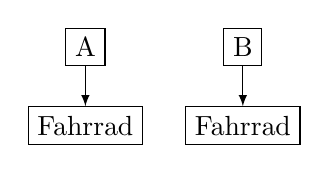
\begin{tikzpicture}[baseline=(A.base)]
			\node [draw, rectangle] (A) at (0,1) {A};
			\node [draw, rectangle] (B) at (2,1) {B};
			\node [draw, rectangle] (fhrd1) at (0,0) {Fahrrad};
			\node [draw, rectangle] (fhrd2) at (2,0) {Fahrrad};

			\draw [-latex] (A) -- (fhrd1);
			\draw [-latex] (B) -- (fhrd2);
		\end{tikzpicture}
		\\

	\ex \label{ex:siebeidefhrd_2}
		Sie beide haben ein Fahrrad.
		\medskip

		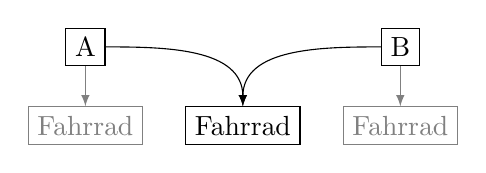
\begin{tikzpicture}[baseline=(A.base)]
			\node [draw, rectangle] (A) at (0,1) {A};
			\node [draw, rectangle] (B) at (4,1) {B};
			\node [draw, rectangle, gray] (fhrd1) at (0,0) {Fahrrad};
			\node [draw, rectangle      ] (fhrd)  at (2,0) {Fahrrad};
			\node [draw, rectangle, gray] (fhrd2) at (4,0) {Fahrrad};

			\draw [-latex] (A) to [out=east, in=north] (fhrd);
			\draw [-latex] (B) to [out=west, in=north] (fhrd);

			\draw [-latex, gray] (A) -- (fhrd1);
			\draw [-latex, gray] (B) -- (fhrd2);
		\end{tikzpicture}
		\\
	\end{xlist}
\end{exe}

Während der Satz in \cref{ex:siebeidefhrd_1} mit gefloatetem Quantor
ausschließlich die Lesart zulässt, bei der beide Parteien jeweils ein Fahrrad
besitzen (distributive Lesart), lässt das Beispiel in \cref{ex:siebeidefhrd_2}
zusätzlich die Interpretation zu, nach der beide Parteien gemeinsam ein Fahrrad
besitzen (kollektive Lesart). Zusätzliche Betonung des Quantors kann in diesem
Fall zwar zur Disambiguierung beitragen (\emph{Sie \emph{beide} haben ein
Fahrrad} = distributiv), ist aber bei der rein textlichen Wiedergabe von Sprache
ohne spezielle Markierung nicht nachvollziehbar.

\phantomsection
\label{phsec:hebrqf}
Die bisher referierten Artikel diskutieren Floating Quantifiers im Rahmen von
Government and Binding \autocite{chomsky1981}. Wie könnte eine Adaption in die
LFG aussehen? Diesen Versuch unternimmt \citet{spector2009} in Rückgriff auf
\citet{shlonsky1991} für das Ivrit, siehe \cref{ex:hebrqf,fig:hebrqf}. Anders
als im Deutschen oder im Französischen kongruiert der gefloatete Quantor
(\fw{kol} `alle') dort nicht bloß, sondern beinhaltet ein klitisches Pronomen,
das mit dem Quantifizierten koindiziert ist.%
%
	\footnote{Im Sinne der Grammatikalisierungs\-theorie nach
		\citet{lehmann2015} stellt Klitisierung eine Vorstufe von Kongruenz dar
		\autocite[vgl.][44]{lehmann2015}.%
	}

\begin{exe}
\ex \label{ex:hebrqf}
	\langinfo%
		{Ivrit}
		{}
		{\cite[nach][522, 537]{spector2009}}\\
	\gll ha-yeladim halxu kulam la-yam \\
		\textsc{def}=children[\textsc{3pl.m}]$_i$ went all=\textsc{3pl.m}$_i$
			to=sea.\textsc{def} \\
	\trans `The children went all to the sea.'
\end{exe}

\begin{figure}
	\begin{forest} shorter edges, narrower nodes, italic leaves, align text
	[IP\mysn{hebrqf_IP}
		[NP\mysn{hebrqf_NP}
			[\xhead{N}
				[ha-yeladim]
			]
		]
		[\xbar{I}
			[\xhead{I}
				[halxu]
			]
			[S%\mysn{hebrqf_S}
				[QP\mysn{hebrqf_QP}
					% [\xbar{Q}
						[\xhead{Q}
							[kulam]
						]
					% ]
				]
				[VP%\mysn{hebrqf_VP}
					[PP\mysn{hebrqf_PP}
						[la-yam, roof]
					]
				]
			]
		]
	]
	%
	\node [avmcontainer, font=\footnotesize] {
		\avm{\tikzmark{hebrqf_f}[
			top	& \tikzmark{hebrqf_top}[
				pred	& `child' \\
				def		& $+$ \\
				num		& \textsc{pl} \\
			] $i$
			\smallskip \\
			%
			subj	& \tikzmark{hebrqf_subj}[
				pred	& \astruct{all}{\ups{obj}} \\
				obj	& [
					pred	& $pro$ \\
					pers	& 3 \\
					gend	& \textsc{m} \\
					num		& \textsc{pl} \\
				] $i$\enspace \\
			]
			\smallskip \\
			%
			pred	& \astruct{went}{\ups{subj}, \ups{\Oblq{dir}}}
			\smallskip \\
			%
			\Oblq{dir}	& \tikzmark{hebrqf_obl}[
				pred	& \astruct{to}{\ups{obj}} \\
				obj	& [
					pred	& `sea' \\
					def		& $+$ \\
					num		& \textsc{sg} \\
				] \\
			] \\
		]}
	};
	\end{forest}
	\begin{tikzpicture}[remember picture, overlay]
		\draw [myarrow]
			([yshift=.5ex]{pic cs:hebrqf_IP})
				to [out=east, in=west]
			([yshift=.5ex]{pic cs:hebrqf_f});
		% \draw [myarrow]
		% 	([yshift=.5ex]{pic cs:hebrqf_S})
		% 		to [out=east, in=west]
		% 	([yshift=.5ex]{pic cs:hebrqf_f});
		% \draw [myarrow]
		% 	([yshift=.5ex]{pic cs:hebrqf_VP})
		% 		to [out=east, in=west]
		% 	([yshift=.5ex]{pic cs:hebrqf_f});
		%
		\draw [myarrow]
			([yshift=.5ex]{pic cs:hebrqf_NP})
				to [out=east, in=west]
			([yshift=.5ex]{pic cs:hebrqf_top});
		\draw [myarrow]
			([yshift=.5ex]{pic cs:hebrqf_QP})
				to [out=east, in=west]
			([yshift=.5ex]{pic cs:hebrqf_subj});
		%
		\draw [myarrow]
			([yshift=.5ex]{pic cs:hebrqf_PP})
				to [out=east, in=west]
			([yshift=.5ex]{pic cs:hebrqf_obl});
	\end{tikzpicture}
	\caption{Analyse des Satzes \fw{Ha-yeladim halxu kulam la-yam} `Die Kinder
		fuhren alle ans Meer'}
	\label{fig:hebrqf}
\end{figure}

\citet[533--534]{spector2009} kommt ähnlich wie \citet[29]{pittner1995} zu dem
Schluss, dass der gefloatete Quantor eine eigenständige NP darstellt. Die
Topikalisierung des Quantifizierten werde durch die Distanzstellung des
Quantors angezeigt; die Konstruktion sei dadurch besonders markiert. Beide NPs,
\textsc{top} und \textsc{subj}, sind in \citeauthor{spector2009}s Analyse durch
Koindizierung verbunden, werden aber nicht in der F-Struktur miteinander
vereinigt \autocite[vgl.][99]{bresnanetal2016}.

Die Analysen von \citet{shlonsky1991,spector2009} für das Ivrit könnten
insofern für die Analyse des Deutschen relevant sein, als
\citet[179]{merchant1996} eine Ähnlichkeit zwischen dem hebräischen \fw{kol}
`alle' und dem deutschen \fw{alle} bezüglich des Auftretens von Flexion in
Abhängigkeit der Stellungsvariante vermerkt: Die Kongruenzendung fehlt, wenn
der Quantor einer definiten NP vorangeht: \fw{all die X} aber \fw{alle X}. Der
Fall von \fw{die beiden X} und \fw{beide X} würde eine separate Diskussion
benötigen. Nachfolgend möchte ich einige vorläufige Überlegungen zur
Modellierung der Situation im Mittelhochdeutschen anstellen.

Während im modernen Standarddeutschen Determinierer und Adjektive normalerweise
links vom Substantiv stehen, können Adjektive im Mittelhochdeutschen
auch rechts davon auftreten \autocite[185--186, 237--243]{ksw2}, selten auch
Determinierer wie Possessivartikel, \norm{dehėin} `kein' und \norm{bėide}
\autocite[515--517, 551--552, 623--624]{ksw2}. Im hier ausgewerteten Material
liegen immerhin zwanzig Fälle im \CAO{} und drei in der \KC{}
mit nachgestelltem \norm{bėide} hinter einem einfachen Plural-Substantiv vor
\cref{ex:beidepost_2}.


\begin{exe}
	\ex \label{ex:beidepost_2}
		\gll ſo man die iargezit beidú begat \\
			so man die Jahrestag[\textsc{acc.pl.\NeutI}]
			beide-\textsc{acc.pl.\NeutI.st} begeht \\
		\trans `wenn man die Jahrestage beide begeht'
			\parencites%
				(Nr.~3331, Straßburg und Colmar, 1299)%
				[468:21--22]{cao4}
\end{exe}

Da die LFG ohne Transformationen auskommt (also keine Verschiebungen von
syntaktischen Einheiten auf einer abstrakten Ebene wie in \cref{fig:qfgg}
angenommen werden), bietet sich für die Lesart mit Kontaktstellung in
\cref{fig:beidepost_2cont} an, \norm{die} (\xhead{D}) und \norm{bėide}
(\xhead{Q}) als funktionale Ko-Köpfe von \norm{jārƶīt} `Jahrestag' (\xhead{N})
zu behandeln.%
%
	\footnote{Artikel und Quantor sind im ursprünglichen Beispiel nicht
		kongruent, insofern \norm{jārƶīt} entweder feminin oder neutral belegt
		ist \autocite[s.\,v.~\fw{jârzît}]{lexer:mhdhwb}. Der Artikel \norm{die}
		flektiert maskulin-feminin, der Quantor \norm{bėidiu} dagegen neutral.
		Neutrum in Bezug auf einen unbelebten Referenten lässt sich als
		semantische Kongruenz interpretieren, was die Lesart in
		\cref{fig:beidepost_2dist} mit pronominal verwendetem \norm{bėidiu}
		plausibler macht.}

\begin{figure}
	\begin{forest} narrower nodes, italic leaves, align text
	[VP
		[\anno{VP}
			[{\anno[\pass{obj}]{DP\mysn{beidepost2c_DP}}}
				[\anno{\xhead{D}}
					[die]
				]
				[\anno{QP\mysn{beidepost2c_QP}}
					[\anno{NP\mysn{beidepost2c_NP}}
						[\anno{\xhead{N}}
							[jārƶīt]
						]
					]
					[\anno{\xhead{Q}}
						[bėide]
					]
				]
			]
		]
		[\anno{\xhead{V}}
			[begāt]
		]
	]
	%
	\node [avmcontainer] {
		\avm{%
		\tikzmark{beidepost2c_f}$f:$ [
			obj	& \tikzmark{beidepost2c_obj}[
				def	& $+$ \\
				pred	& `Jahrestag' \\
				case	& \textsc{acc} \\
				num		& \textsc{pl} \\
				gend	& \textsc{f} \\
				anim	& $-$ \\
				quant	& [
					pred	& `beide' \\
				] \\
			] \\
			%
			pred	& \astruct{begehen}{\ups{subj}, \ups{obj}} \\
		]}
	};
	\end{forest}
	\begin{tikzpicture}[remember picture, overlay]
	\draw [myarrow]
		([yshift=.5ex]{pic cs:beidepost2c_NP})
		to [out=east, in=west]
		([yshift=.5ex]{pic cs:beidepost2c_obj});
	\draw [myarrow]
		([yshift=.5ex]{pic cs:beidepost2c_QP})
		to [out=east, in=west]
		([yshift=.5ex]{pic cs:beidepost2c_obj});
	\draw [myarrow]
		([yshift=.5ex]{pic cs:beidepost2c_DP})
		to [out=east, in=west]
		([yshift=.5ex]{pic cs:beidepost2c_obj});
	\end{tikzpicture}
	\caption{Analyse des Satzfragments \norm{die jārƶīt bėide begāt} `die beiden Jahrestage begeht'}
	\label{fig:beidepost_2cont}
\end{figure}

Basierend auf der Analyse von \citet{spector2009} für das Ivrit dient das
Schema in \cref{fig:beidepost_2dist} als Arbeits\-hypothese für die Lesart mit
gefloatetem Quantor. Parallel zu \textsc{subj} und \textsc{top} werden hier die
Rollen \textsc{obj} und \textsc{foc} für \norm{bėidiu} und die dazugehörige DP
angenommen. Die aufeinander bezogenen Teile ($g$ und $h$) sind koindiziert
($i$), um die anaphorische Funktion von \norm{bėide} zu erfassen.%
%
	\footnote{Die Annotationsform \q{\uncertain{$x$}{$a$}~\req~$v$} in
		\cref{fig:beidepost_2dist} bedeutet, dass entsprechend der Flexion der
		annotierten Wortform außerhalb des lokalen Funktionskerns (hier $h$)
		eine grammatische Funktion $x$ als Controller existiert, die ein
		Attribut $a$ besitzt, das den Wert $v$ für sein Target voraussetzt
		(\fw{inside-out functional uncertainty};
		\cite[66--70]{bresnanetal2016}).}
%
Eine eingehendere Diskussion der Konstruktion müsste auf die Bindungsrelation,
etwa im Vergleich zu Reflexivpronomina, und gegebenenfalls funktionale
Präzedenz eingehen \autocite[vgl.][213, 254--285]{bresnanetal2016}. Auch für
den in \cref{ex:floatsubj_3} illustrierten Unterschied in der Akzeptabilität
von \textit{Alle mögen sie/*die Kinder Schokolade} könnte dies eine Rolle
spielen.

\begin{figure}
	\begin{forest}
		shorter edges,
		narrower nodes,
		italic leaves,
		align text
	[VP
		[\anno{VP}
			[{\anno[\pass{foc}]{DP\mysn{beidepost2d_DP}}}
				[\anno{\xhead{D}}
					[die]
				]
				[\anno{NP\mysn{beidepost2d_NP}}
					[\anno{\xhead{N}}
						[jārƶīt]
					]
				]
			]
			[\anno{VP}
				[{\anno[\pass{obj}]{QP\mysn{beidepost2d_QP}}}
					[\anno{\xhead{Q}}
						[bėidiu, name=beidiu, minimum width=5em]
					]
				]
			]
		]
		[\anno{\xhead{V}}
			[begāt]
		]
	]
	%
	% Annotation des Knotens zu breit, als dass die AVM noch hinpasst
	\node at (beidiu) [below=1ex] {
		\smaller[2]\upshape\tabcolsep=.5ex%
		\begin{tabular}[t]{@{} l l l @{}}
			\uncertain{$x$}{case}	& \req & \textsc{acc} \\
			\uncertain{$x$}{num}	& \req & \textsc{pl} \\
			\uncertain{$x$}{gend}	& \req & \textsc{n} \\
			$\lor$ \uncertain{$x$}{anim} & \req & $-$ \\
		\end{tabular}%
	};
	%
	\node [avmcontainer] {
		\avm{%
		\tikzmark{beidepost2d_f}$f:$ [
			foc	& \tikzmark{beidepost2d_foc}$g:$ [
				def		& $+$ \\
				pred	& `Jahrestag' \\
				case	& \textsc{acc} \\
				num		& \textsc{pl} \\
				gend	& \textsc{f} \\
				anim	& $-$ \\
			]~$i$ \smallskip \\
			%
			obj	& \tikzmark{beidepost2d_obj}$h:$ [
				pred	& `beide' \\
			]~$i$ \\
			%
			pred	& \astruct{begehen}{\ups{subj}, \ups{obj}} \\
		]}
	};
	\end{forest}
	\begin{tikzpicture}[remember picture, overlay]
	\draw [myarrow]
		([yshift=.5ex]{pic cs:beidepost2d_NP})
		to [out=east, in=west]
		([yshift=.5ex]{pic cs:beidepost2d_foc});
	\draw [myarrow]
		([yshift=.5ex]{pic cs:beidepost2d_QP})
		to [out=east, in=west]
		([yshift=.5ex]{pic cs:beidepost2d_obj});
	\draw [myarrow]
		([yshift=.5ex]{pic cs:beidepost2d_DP})
		to [out=east, in=west]
		([yshift=.5ex]{pic cs:beidepost2d_foc});
	\end{tikzpicture}
	\caption{Analyse des Satzframents \norm{die jārƶīt bėidiu begāt} `die Jahrestage beide begeht'}
	\label{fig:beidepost_2dist}
\end{figure}

Die Schemata in \cref{fig:beidepost_2cont,fig:beidepost_2dist} zeigen außerdem,
dass die Nachstellung des Quantors tendenziell zu syntaktischer Ambiguität
führt. In den hier gesammelten Daten tritt das Problem vor allem bei den
zahlreichen Belegen für \norm{si bėide} auf, wenn \norm{si} im Mittelfeld
steht \cref{ex:sibeideambig}. Kontaktstellung ist also nicht gleich
Kontaktstellung, da auch in Kontaktstellung ein gefloateter Quantor vorliegen
kann. \citet[623--624]{ksw2} benennen dieses Problem ebenfalls und zählen
\blockquote{solche Fälle immer als attributiv nachgestellt}, also wie in
(\ref{ex:sibeideambig}a) dargestellt.

\begin{figure}
\begin{forest}
	shorter edges,
	italic leaves,
	align text,
	[\anno{VP}
		[{\anno[\pass{gf}]{QP}}
			[\anno{DP}
				[\anno{\xhead{D}}
					[si]
				]
			]
			[\anno{\xhead{Q}}
				[bėide]
			]
		]
		[\anno{\xbar{V}}
			[\dots]
		]
	]
\end{forest}
\hspace{2em}
\begin{forest}
	shorter edges,
	italic leaves,
	align text,
	[\anno{VP}
		[{\anno[\pass{df}]{DP}}
			[\anno{\xhead{D}}
				[si]
			]
		]
		[\anno{VP}
			[{\anno[\pass{gf}]{QP}}
				[\anno{\xhead{Q}}
					[bėide]
				]
			]
			[\anno{\xbar{V}}
				[\dots]
			]
		]
	]
\end{forest}
\caption{Zwei Varianten von oberflächlicher Kontaktstellung}
\label{ex:sibeideambig}
\end{figure}

\section{Die Kongruenzhierarchie}
\label{sec:kongrhier}

Die von \citet{corbett1979} formulierte Kongruenzhierarchie (\fw{agreement
hierarchy}) basiert auf dem typologischen Vergleich einer Reihe
(indo-)europäischer Sprachen, die sowohl formale als auch semantische Kongruenz
zulassen.%
%
	\footnote{Dies sind: Deutsch, Englisch, Französisch, Lateinisch, Russisch,
	Spanisch \citep[214--215]{corbett1979}. Die Stichprobe ist durch die
	Beschränkung auf große europäische Sprachen typologisch nicht
	repräsentativ. \citet[218]{corbett2006} listet weitere Sprachen auf -- auch
	nicht-indoeuropäische --, für die seitdem Untersuchungen durchgeführt
	wurden.}
%
Das Ergebnis der Studie ist, dass mit wachsender \q{syntaktischer Distanz}
zwischen Controller und Target die Wahrscheinlichkeit für das Auftreten von
semantischer statt formaler Kongruenz steigt \citep[218--223]{corbett1979}.
\citet[204]{corbett1979} formuliert die Kongruenzhierarchie folgendermaßen:

\begin{exe}
\ex attributive > predicate > relative pronoun > personal pronoun
\end{exe}

Je weiter links ein Target einzuordnen ist, desto höher ist die
Wahrscheinlichkeit, dass formale Kongruenz auftritt; je weiter rechts, desto
höher die Wahrscheinlichkeit für semantische Kongruenz. Die Abfolge ist
monoton: Wenn bei einem Targettyp semantische Kongruenz möglich ist, ist dies
auch bei allen Targettypen rechts von ihm möglich. Da für das Deutsche manche
von \citeauthor{corbett1979}s Kategorien für den von ihm untersuchten
Genusausgleich relevanter als andere sind (Genus ist kein Merkmal der
Verbalflexion; Possessivpronomen kongruieren doppelt), schlägt
\citet[193]{fleischer2012} mit einem Blick speziell auf die Genus-Kongruenz
folgende Konkretisierung vor:

\begin{exe}
\ex Artikel, attributives Demonstrativpronomen \\
	\hspace*{1em} > andere attributive Relationen \\
	\hspace*{2em} > Relativpronomen \\
	\hspace*{3em} > anaphorisches Demonstrativpronomen, Personalpronomen \\
	\hspace*{4em} > anaphorisches Possessivpronomen
\end{exe}

Er betont den Sonderstatus des Relativpronomens, das sowohl eine anaphorische
als auch eine attributive Funktion hat, und merkt weiterhin an, dass das
\blockcquote[194]{fleischer2012}{attributiv verwendete Adjektiv und Partizip
\textelp{} im Spätalthochdeutschen und Mittelhochdeutschen auch mit
semantischer Kongruenz auf\textins{tritt}, umgekehrt zeigt das Personalpronomen
in älteren althochdeutschen und vor allem in den jüngsten neuhochdeutschen
Texten auch formale Kongruenz}.

Bezogen auf die syntaktische Motivation der statistisch erarbeiteten
Erkenntnisse schreibt \citet[216]{corbett1979}, dass attributive Kongruenz auf
die einfachen Phrase beschränkt sei, prädikative Kongruenz die Phrase
überschreite doch auf den Teilsatz beschränkt bleibe, während Personalpronomen
nicht auf den Satz der Instanz beschränkt sei, die die Kongruenzbeziehung
kontrolliert.%
%
	\footnote{\foreignblockcquote{english}[216]{corbett1979}{%
		\textins*{A}ttributive agreement represents agreement within the simple
		phrase, predicative agreement goes beyond the phrase but is restricted
		to the clause, the agreement of the relative pronoun goes beyond the
		clause but is restricted to the sentence, while the personal pronoun is
		not restricted to the sentence of the item controlling agreement}.}

Die Kernthese von \citet{wechslerzlatic2003} ist daher, dass formale Kongruenz
bei Attributen zu erwarten ist, da innerhalb der NP \textsc{concord} das
entscheidende Kongruenzmerkmal darstellt. Hingegen ist semantische Kongruenz
bei Personalpronomen außerhalb der bindenden NP deshalb mit höherer
Wahrscheinlichkeit zu erwarten, weil Pronomen über den referenziellen
\textsc{index} an ihren Referenten gebunden sind
\citep[89--91]{wechslerzlatic2003}. Die Autoren argumentieren also für eine
Korrelation zwischen der Distribution von Kongruenz zeigenden Wortarten, deren
syntaktischer Lokalität sowie den anwendbaren Kongruenz\-merkmalen.

\cite[89]{wechslerzlatic2003} erklären weiter, dass Personalpronomen auch
deiktisch oder exophorisch verwendet werden können, also mit Verweis auf
außersprachliche Referenten, ohne dass diese zunächst innersprachlich verankert
wurden. In diesen Fällen komme entweder grammatische oder pragmatische
Kongruenz zum Zuge, letztere speist sich aus der Semantik des Bezeichneten.
Relativpronomina seien dagegen immer anaphorisch gebunden -- wobei sich die
Autoren hier vermutlich auf den innersprachlichen Kontext beziehen -- und
kongruieren in \textsc{index}-Merkmalen, möglicherweise auch in
\textsc{condord}-Merkmalen, da sie NP-intern auftreten. Aufgrund induktiver
Kriterien ergibt sich das Schema in \cref{fig:theoagrdist}.

\begin{figure}
\centering
\begin{tabularx}{\linewidth}{>{\itshape}c l C C C C C}
\toprule
%
	& %
	& \textit{formal}
	& %
	& $\to$
	& %
	& \textit{semantisch}
	\\

\cmidrule{3-7}

%
	& %
	& \multicolumn{3}{c}{grammatisch}
	& %
	& \multirow{2}{*}{\makecell{prag-\\ matisch}}
	\\

\cmidrule{3-5}

%
	& %
	& \textsc{concord}
	& %
	& \textsc{index}
	& %
	& %
	\\

\toprule

lokal
	& Attribute von \xhead{N}
	& \chk
	& %
	& %
	& %
	& %
	\\

\multirow{3}{*}{$\downarrow$}
	& sekundäres Prädikat
	& \chk
	& %
	& %
	& %
	& %
	\\

%
	& Relativpronomen
	& \chk
	& und
	& \chk
	& %
	& %
	\\

%
	& primäres Prädikat
	& %
	& %
	& \chk
	& %
	& %
	\\

distal
	& Personalpronomen
	& %
	& %
	& \chk
	& oder
	& \chk
	\\

\bottomrule
\end{tabularx}
\caption[Interaktion von Kongruenztyp und Wortartensyntax]{Interaktion von
Kongruenztyp und Wortartensyntax in Erweiterung von
\citet[84]{wechslerzlatic2003}}
\label{fig:theoagrdist}
\end{figure}

Es sei darauf hingewiesen, dass dieses Schema keinen Anspruch hat,
allgemeingültige Aussagen zu treffen, sondern lediglich dazu dient, theoretisch
begründete Voraussagen zur Ausprägung von Kongruenz in den jeweiligen
syntaktischen Konstellationen zu machen. Dies ersetzt keinesfalls die deduktive
Analyse von Daten, wie sie in \cref{ch:caoanalyse,ch:kcanalyse} vorgenommen
wird.

\section{Erweiterter Konjunktionsbegriff}
\label{sec:erwkonjbegr}

Neben Fällen, in denen sich \fw{beide} direkt oder indirekt auf zwei mit
\fw{und} verbundene Konjunkte bezieht (zum Beispiel \q{\textsc{substantiv}
\fw{und} \textsc{substantiv}}), gibt es vereinzelt Kontexte, in denen die
kombinierten Controller nach syntaktischen Kriterien keine Konjunkte im
formalen Sinn darstellen \autocite[vgl.~auch][247--248]{askedal1973}.
Nichtsdestoweniger können zwei formal getrennte Controller $i$ und $j$ im
Diskurs existieren, auf die sich \norm{bėide} `beide' als Target
gleichermaßen bezieht. Dies ist in der Belegstelle in \cref{ex:disjointctrl_1}
der Fall, in der es um ein Geschäft geht, das \fw{Agneſ} und \fw{Lukas}
gemeinsam getätigt haben. Sie sagen \lit{bedi} `beide (\textsc{n.pl})' aus, die
Zahlung erhalten zu haben.%
%
	\footnote{In der ausgewerteten Stichprobe tritt \lit{be(i)di} wie an der in
		\cref{ex:disjointctrl_1} zitierten Stelle auch an folgenden weiteren
		Stellen ausschließlich bei der Kombination von männlichen und
		weiblichen Controllern auf: \notecite[\pno~81, 124.23]{cao1}
		(\cite{cao1}; Kl.~Tennenbach, Kr.~Emmendingen, 1264);
		\notecite[\pno~190, 205.38--39]{cao1} (\cite{cao1}; Basel, 1273);
		\notecite[\pno~N~230, 175.14]{cao5} (\cite{cao5}; Straßburg, 1283). Bei
		der Belegannotation wurde davon ausgegangen, dass \lit{be(i)di} eine
		entrundete Variante der neutralen Form \norm{bėidiu} darstellt, die in
		diesen Kontexten vorherrscht \autocites(siehe auch
		\cref{sec:caoalemschwa})[vgl.][41]{paul2007}. Die Grafie der
		betreffenden Urkunden fällt nicht dadurch auf, dass dort regelmäßig
		\lit{-i} für einen unbetonten Nebensilbenvokal geschrieben wird.
		\label{fn:caoalemschwa}}

\begin{exe}
\ex\label{ex:disjointctrl_1}
	\setlength{\glossglue}{6pt plus 2pt minus 2pt}
	\gll das vur Agneſ$_i$ mit hern Lukas$_j$ hant \textelp{}
			het gegeben ze coͧffenne \textelp{} vn̄ hant bedi$_{i+j}$ veriehen,
			daſ ſie gewert ſint dis ſilberſ \\
		dass Frau Agnes[\textsc{nom.sg.\FemF}] mit Herrn
			Lukas[\textsc{dat.sg.\MascM}] Hand {} hat gegeben zu kaufen {} und
			haben beide-\textsc{nom.pl.n\subMF.st} ausgesagt dass sie gewährt
			sind dieses Silbers \\
		\trans `dass Frau Agnes mit Herrn Lukas' Hand \textelp{} hat zum
			Kauf gegeben \textelp{} und haben beide ausgesagt, dass ihnen das
			Silber gezahlt wurde.'
			\parencites%
				(Nr.~N~202, Straßburg, 1281)%
				[156:11--16]{cao5}
\end{exe}

Auf formaler Ebene werden \fw{Agneſ} und \fw{Lukas} aber nicht koordiniert.
Vielmehr liegt \lit{mit hern Lukas hant} `mit Herrn Lukas' Hand' eine
adverbiale Präpositionalphrase vor, in der \lit{Lukas} seinerseits ein
Genitivattribut zu \lit{hant} `Hand' darstellt. Trotz allem sind beide
Personen damit im Diskurs verankert, sodass im weiteren Verlauf Verben wie
\lit{hant} `haben (\textsc{3pl.ind.prs})', Pronomina wie \norm{ſie} `sie
(\textsc{pl})' und damit auch \lit{bedi} `beide' auf sie gemeinsam Bezug nehmen
können.

Während in \cref{ex:disjointctrl_1} die beiden Controller in unterschiedlichen
Satzgliedern desselben Satzes stehen, ist die Verbindung der Controller in
\cref{ex:disjointctrl_2} unter formalen Kriterien noch lockerer. So bezieht sich
\lit{ſi beidv̍} `sie beide (\textsc{n})' dort gleichermaßen auf
\lit{Mehthilt} und ihren Mann \lit{Heinrich\textdel{}}. Letzterer wird
syntaktisch getrennt in einem eingeschobenen, unabhängigen Temporalsatz
genannt.

\begin{exe}
\ex\label{ex:disjointctrl_2}
	\gll dv̓ vorgenante fro Mehthilt$_i$ / vor e ſi$_i$ den
			vorgenanten Heinrichen$_j$ neme \textelp{} vn̄ ſo
			ſi$_{i+j}$ beidv̍$_{i+j}$ ſterbent \textelp{}
			% ſo iſt daſ vorgenante guͦt \textelp{} {dem ſelben} ſpittal vn̄
			% den dv̓rftigen lidig
			\\
		die vorgenannt Frau Mechthild[\textsc{nom.sg.\FemF}] {} vor ehe
			\textsc{3sg.\FemF.nom} den vorgenannten
			Heinrich-\textsc{acc.sg.\MascM} nahm {} und so
			\textsc{3pl.\subMF.nom} beide-\textsc{nom.pl.\NeutMF.st} sterben {}	
			% so ist das vorgenannte Gut {} demselben Spital und den
			% Bedürftigen ledig
			\\
		\trans `Die vorgenannte Frau Mechthild, bevor sie den
			vorgenannten Heinrich \textins{zum Mann} nahm \textelp{} Und wenn
			sie beide sterben \textelp{}%
			% , fällt das vorgenannte Gut an dasselbe Spital und die
			% Bedürftigen zurück.
			'
			\parencites%
				(Nr.~2008, Freiburg i.\,Br., 1294)%
				[253:30--39]{cao3}
\end{exe}

Innerhalb des Temporalsatzes wird Mechthild zwar durch das Pronomen \lit{ſi}
`sie' vertreten, doch auch hier liegt keine Konjunktion vor, da \lit{ſi}
das Subjektspronomen und Heinrich das Objekt von \lit{neme} `nahm'
darstellt. Beide Controller werden zwar syntaktisch unabhängig voneinander im
Diskurs etabliert, stehen aber für den kombinierten Bezug durch Pronomen wie
\norm{si} `sie (\textsc{pl})' und damit auch für \norm{bėide}
`beide' zur Verfügung.

Im Sinne eines erweiterten Konjunktionsbegriffs werden im Folgenden auch
\norm{bėide}-Targets wie die in \cref{ex:disjointctrl_1,ex:disjointctrl_2}
berücksichtigt, obwohl ihre Controller formal nicht mit einer Konjunktion
verbunden sind. Was in diesen Fällen zählt, ist, dass sich das jeweilige Target
auf semantischer Ebene gleichzeitig auf zwei Controller bezieht, indem die
Controller im Kontext verankert -- indiziert -- sind.

\chapter{Forschungsüberblick}
\label{ch:forschungsueberblick}

\section%
	{\norm{Bėide} als Quantor -- \norm{X unde Y \dots\ (si) bėide/bėidiu}}
\label{sec:ovwbeidequant}

Bei dem Kongruenzphänomen, das in dieser Studie anhand des Quantors
\norm{bėide} `beide (\textsc{nom+acc.pl.m+f.st})' beziehungsweise \norm{bėidiu}
`beide (\textsc{nom+acc.pl.n.st})' in mittelhochdeutschen\il{Mittelhochdeutsch}
Quellen untersucht wird, handelt sich um eine bekannte Eigenheit der
germanischen\il{Germanisch} Sprachen. Diese zeigt sich insbesondere in den
älteren Sprachstufen, ist darüber hinaus aber noch im modernen
Isländischen\il{Isländisch} \autocites[283]{corbett1991}[569]{wechsler2009} und
Färöischen\il{Färöisch} \autocite[225--226]{thrainsson2004} erhalten geblieben.
In \REF{ex:germbeide} werden zur Illustration einige Beispiele aus historischen
Quellen präsentiert.%
%
	\footnote{Die Stellen sind \citet[12]{askedal1973} entnommen, vgl.~auch
		\citet{hock2008,hock2009}.}

\begin{exe}
\ex \label{ex:germbeide}
	\begin{xlist}
	\ex \label{ex:germbeide_1}
		\langinfo%
			{Gotisch}
			{}
			{\cite[nach][]{projectwulfila2004}}
			\\
		% Digi: https://www.alvin-portal.org/alvin/imageViewer.jsf?dsId=ATTACHMENT-0147&pid=alvin-record:60279
		\gll Iosef \textelp{} miþ Mariin \textelp{} warþ þan,
				miþþanei þo wesun jainar \textelp{} \\
			Josef[\textsc{nom.sg.\MascM}] {} mit Maria-\textsc{dat.sg.\FemF} {}
				wurde dann während \textsc{dem.nom.pl.\NeutMF} waren dort {} \\
		\trans `Josef \textelp{} mit Maria \textelp{} Während diese dort
			waren, wurde dann \textelp{}'
			(%
				\iai{Wulfila}, \tit{Bibel}: Lk~2,4--6;
				vgl. Uppsala, Universitätsbibl., MS~DG~1: 124r,1--9%
			)

	\ex \label{ex:germbeide_2}
		\langinfo%
			{Altwestnordisch}
			{}
			{\cite[nach][73]{neckelkuhn1962}}\\
		% Digi: https://handrit.is/manuscript/view/is/GKS04-2365/31?iabr=on#page/11v
		\gll Gerðr qvað: \textelp{} \\
			Gerðr[\textsc{nom.sg.\FemF}] sprach {} \\
		\gll né við Freyr, meðan occart fiǫr lifir, \\
		% ne viþ freẏ meꝥ occart fior lif͛
			noch \textsc{1du\subMF.nom} Freyr[\textsc{nom.sg.\MascM}] während
				\textsc{1du.gen-nom.sg.\NeutMF} Körper lebt \\
		\gll byggiom bæði saman. \\
		% byɢiõ bęði ſaman.
			wohnen-\textsc{1pl.ind.prs} beide-\textsc{nom.pl.\NeutMF.st} zusammen \\
		\trans `Gerðr sprach: \textelp{} noch Freyr und ich, so
			lange wir leben, beide zusammen wohnen.'%
		%
			\footnote{Für die Glossierung danke ich Svenja Walkenhorst
				(Marburg). \citet[53]{terry1990} übersetzt frei:
				\foreignblockquote{english}{Frey will never
				enjoy my favor as long as we're both alive}.}
		%
			(%
				\tit{Edda}: For Skírnis 20,4--5;
				vgl. Reykjavík, Stofnun Árna Magnússonar, GKS 2365 4to: 22,18--19%
			)

	\ex \label{ex:germbeide_3}
		\langinfo%
			{Altenglisch}
			{}
			{\cite[nach][27]{krapp1931}}\\
		% Digi: https://digital.bodleian.ox.ac.uk/objects/d5e3a9fc-abaa-4649-ae48-be207ce8da15/
		% \gll ⁊ ƿit hér baru ſtandað. \\
		\gll and wit her baru standað \\
			und \textsc{1du\subMF.nom} hier nackt-\textsc{nom.pl.\NeutMF.st}
				stehen \\
		\trans `und wir beide \textins{=~Adam (\MascM) und Eva (\FemF)}
			hier nackt stehen.'
			(%
				\iai{Cædmon}, \tit{Genesis}: V.~811;
				vgl. Oxford, Bodleian Lib., Cod.~Junius 11: 38,9--10%
			)			

	\ex \label{ex:germbeide_4}
		\langinfo%
			{Altsächsisch}
			{}
			{\cite[nach][35]{sievers1878}}\\
		\gll Giuuitun im tho thiu godun tuue \\
			heiligten ihm da \textsc{dem.nom.pl.\NeutMF} gut-\textsc{nom.pl.wk}
			zwei[\textsc{\NeutMF}] \\
		\gll Ioseph endi Maria \\
			Josef[\textsc{nom.sg.\MascM}] und Maria[\textsc{nom.sg.\FemF}] \\
		\gll bediu fon Bethleem \\
			beide-\textsc{nom.pl.\NeutMF.st} von Bethlehem \\
		\trans `Da beteten ihn diese guten zwei an, Josef und Maria, die beiden
			von Bethlehem.'
			(%
				\tit{Heliand}: V.~458--459;
				vgl. München, Bayerische Staatsbibl., Cgm~25: 7v,5--6%
				% [\cite[8827]{hsc}]
			)

	\ex \label{ex:germbeide_5}
		% Althochdeutsch (Wien, ÖNB, Cod. 2687: 15v,20):
		% \gll Vuárun ſẹ\textsup{iu} béthịu góte filu drúdịu \\
		\langinfo%
			{Althochdeutsch}
			{}
			{\cite[nach][15v]{kleiberhellgardt2004}}\\
		\gll Vuárun ſiu béthịu góte fılu drúdịu \\
			Waren \textsc{3pl.nom.pl.\NeutMF} beide-\textsc{nom.pl.\NeutMF.st}
				Gott viel lieb-\textsc{nom.pl.\NeutMF.st} \\
		\trans `Sie beide \textins{=~Zacharias (\textsc{\MascM}) und
			Elisabeth (\textsc{\FemF})} waren Gott sehr lieb.'
			(%
				\iai{Otfrid von Weißenburg}, \tit{Evangelienbuch}: I.4,5;
				vgl. Wien, Österreichische Nationalbibl., Cod.~2687: 15v,20%
				% [\cite[6494]{hsc}]
			)
		\\
	\end{xlist}
\end{exe}

In allen Fällen liegen Paare aus Mann und Frau vor; sich auf diese gemeinsam
beziehende Wortformen weisen jeweils das Neutrum auf. Auch wenn in
\REF{ex:germbeide_1} und \REF{ex:germbeide_3} mit \lit{þo} `diese
(\textsc{pl.\NeutMF})' beziehungsweise \lit{baru} `nackt
(\textsc{pl.\NeutMF})' keine Formen von \fw{beide} betroffen sind,
illustrieren sie durch ihre neutrale Kongruenz dennoch das Phänomen.

Mit Fokus auf die älteren Sprachstufen des Deutschen beobachtet dazu bereits
\citeauthor{grimm1848} in der \citetitle{grimm1848}:
\blockcquote[978]{grimm1848}{Da unserm adjectiv und, ausser dem
persönlichen, dem übrigen pronomen die dualform mangelt, so verdient hier
erwogen zu werden, dass unsre syntax mit zwei subjecten verschiednes
geschlechts das adj.\ im pl.~neutr.\ verbindet}. In der \tit{Deutschen
Grammatik}\il{Neuhochdeutsch} wird dieser Gedanke vertieft:
\blockcquote[311--312]{grimm1890}{\textins*{S}ollen adjectiva oder pronomina
auf ein männliches und weibliches subst.\ \emph{zugleich} bezogen werden, so
stehen sie im \emph{neutro}; jene subst.\ mögen vom natürlichen oder bloß
grammatischen geschlecht sein}. An späterer Stelle argumentiert
\citeauthor{grimm1898}, dass für die Kombination von Maskulinum und Femininum
\blockcquote[329]{grimm1898}{der uralte grundsatz \textins{gilt}, daß ein auf
beide zugleich bezügliches pron.\ adj.\ und partic.\ in den \emph{pl.\ des
\mbox{neutr.}} zu stehn kommt, und gerade vorzugsweise bei personen}. Das
Neutrum trete darüber hinaus auch in Abhängigkeit von der Kombination eines
Singulars Maskulinum oder Femininum mit einem Singular Neutrum auf
\autocite[331]{grimm1898}.

Speziell auf das Mittelhochdeutsche\il{Mittelhochdeutsch} bezogen fällt die
Regelangabe bei \citeauthor{paul2007} gewohnt knapp und impressionistisch aus:
\blockcquote[384]{paul2007}{In der Regel steht ein Pron.\ oder Adj.\ im
Pl.~Neutr., wenn es zusammenfassend auf mehrere Subst.\ mit unterschiedlichem
Genus bezogen ist \textelp{}. Es kann aber auch der Pl.~Mask.\ in solchen
Fällen gebraucht werden}. Ähnlich kurz wie \citet{paul2007} formuliert
\citet[39]{behaghel1928}: \blockquote{Das feste Glied besteht aus einer Summe
von Gliedern verschiedenen Geschlechts; es erscheint von alters her das
Attribut\is{Attribut}, das Prädikat und das aufnehmende Pronomen im Neutrum
Pluralis. \textelp{} Doch wird diese aus der Vorzeit überkommene formale
Regelung nicht selten durch die Rücksicht auf das natürliche Geschlecht
durchkreuzt}.

\citet{behaghel1928} scheint also anzunehmen, dass das Neutrum als
Ausgleichsform aufgrund eines formalen, morphosyntaktisch bedingten Mechanismus
erscheine, während die neuere Forschung etwa von \citet{wechslerzlatic2003} und
\citet{wechsler2009} davon ausgeht, dass Gender Resolution ein in der Semantik
begründetes Phänomen darstellt, wie in \chapref{ch:diskussion} zu zeigen sein
wird. Darüber hinaus vermerken auch \citet[188]{dal2014} bloß, dass
\blockquote{\textins*{w}enn mehrere Substantive von verschiedenem Geschlecht
durch Konjunktion verbunden sind, \textelp{} darauf bezogene
Attribute\is{Attribut} und hinweisende Pronomina ursprünglich im Neutr.\ Plur.\
\textins{stehen}}.

Ausführliche Kritik an den Formulierungen von \citet{grimm1890,grimm1898} und
\citet{behaghel1928} sowie von Dal\nocite{dal2014} und Paul\nocite{paul2007},
die auch in den jeweils aktuellen Auflagen
\autocite{dal2014,paul2007} unverändert geblieben sind, übt bereits
\citet[11--15, 195--213]{askedal1973}. Dieser beschäftigt sich mit der
diachronen Entwicklung dieses Phänomens vom Althochdeutschen\il{Althochdeutsch}
bis zur \q{Blütezeit} der mittelhochdeutschen\il{Mittelhochdeutsch} Epik um
1200 \autocites[vgl.][317]{schneidermohr2001}[dazu auch][3--29]{johnson1999}.
Die Essenz seiner Kritik ist, dass bei den genannten Darstellungen

\begin{itemize}
	\item nicht klar zwischen natürlichem und grammatischem Geschlecht (also
		semantischen und formalen Kriterien) unterschieden wird;
	\item die Regelangaben die diachrone Ebene außer Acht lassen;
	\item insbesondere auf die Verbindung von Personen (Animata\is{Animata})
		eingegangen wird, kaum aber auf die von Dingen und Abstrakta
		(Inanimata);
	\item sich die Beschreibung auf die bloße Feststellung von Regel und
		Ausnahme\is{Ausnahme} beschränkt und dabei \isi{Belebtheit} kaum eine
		oder keine Rolle spielt;
	\item als Begründung für die Kongruenzregel entweder nur \q{formale} (das
		heißt morphologische?) Aspekte oder in der Tradition der
		Junggrammatiker die reine Lautentwicklung angeführt werden.
\end{itemize}

\citet{askedal1973} geht es bei seiner Studie nicht nur um
\norm{bėidiu}, sondern um den größeren Kontext des Verlusts der Genusopposition
zwischen Maskulinum-Femininum und Neutrum im Plural
\autocite[169--177]{askedal1973}. Er untersucht dafür hauptsächlich das
Pronominalsystem der fünf Texte: \tit{Tatian}, Otfrids von Weißenburg\ia{Otfrid
von Weißenburg} \tit{Evangelienbuch}, die \tit{Altdeutsche Genesis}, Wolframs
von Eschenbach\ia{Wolfram von Eschenbach}
\tit{Parzival} und Gottfrieds von Straßburg\ia{Gottfried von Straßburg}
\tit{Tristan}. Herausfordernd für eine quantitative Untersuchung ist, dass in
allen Texten trotz ihrer Länge jeweils nur wenige relevante Belege vorliegen
\autocites[187]{askedal1973}[118]{fleischerschallert2011}. Wichtig an
\citeauthor{askedal1973}s Arbeit ist der Versuch, \fw{Gender Resolution} -- die
Auflösung konfligierender Genusmerkmale in der Kongruenz\-morphologie
\autocites(siehe \sectref{sec:gendres}){corbett1983} -- als komplexen
morphosyntaktischen Vorgang aufzufassen, nämlich als eine syntaktische
Operation, die mit semantischen und formalen Merkmalen operiert und in der
Morphologie ihren Ausdruck findet. Leider lässt \citet{askedal1973} eine
übersichtliche Darstellung seiner Daten und Ergebnisse vermissen, sodass ein
direkter Vergleich zwischen seinen einzelnen Teilauswertungen schwierig ist;
eine kurze Zusammenfassung der wichtigsten Erkenntnisse seiner Arbeit bieten
\citet[118--119]{fleischerschallert2011}.

Interessant für die vorliegende Studie ist, dass der \tit{Parzival} und der
\tit{Tristan} bezüglich ihres zeitlichen Überlieferungsschwerpunkts in den
Rahmen der hier untersuchten Texte fallen. \citet[1378]{bumke1999} zufolge kann
als Entstehungszeit für den \tit{Parzival} Wolframs von Eschenbach etwa die
Zeit zwischen 1200 und 1210 angesetzt werden. Die ältesten erhaltenen
Textzeugen werden auf die erste Hälfte des 13.~Jahrhunderts, die jüngsten auf
die Zeit um 1500 datiert
\autocites[1381]{bumke1999}[vgl.~auch][s.\,v.~\textit{Wolfram von Eschenbach:
\tit{Parzival}}]{hsc}. Die Entstehungszeit des \tit{Tristan}-Romans Gottfrieds
von Straßburg\ia{Gottfried von Straßburg} gibt \citet[155]{kuhn1982} mit der
Zeit zwischen 1200 und 1220 an. Er ist uns in Handschriften aus dem frühen
13.~Jahrhundert bis zum letzten Viertel des 15.~Jahrhunderts überliefert
\autocite[vgl.][s.\,v.~\textit{Gottfried von Straßburg: \tit{Tristan}}]{hsc}.

Die Belegverteilung für den \tit{Parzival} und den \tit{Tristan} bei
\citet{askedal1973} wird in \tabref{tab:askbeide} aufgeführt, insofern die
Daten aus dem Fließtext herausgelesen werden konnten. Kontexte mit der
Flexionsendung in Hiatuspositionen und am Zeilenende wurden dabei jeweils nicht
mitgezählt. Das heißt, \citet[89--91]{askedal1973} argumentiert mit Verweis auf
\citet[662--663]{grimm1870}, dass in mittelhochdeutschen\il{Mittelhochdeutsch}
Verstexten im Endreim nie \norm{-iu} zu beobachten ist, stattdessen immer
\norm{-e} gesetzt wird. Des Weiteren mahnt er zur Vorsicht bei Kontexten, in
denen in einem metrisch gebundenen Text eine flektierte Wortform auf Vokal
endet und die nachfolgende mit einem Vokal beginnt. Um einen metrisch glatten
Vers zu produzieren, kann der unbetonte Endvokal der ersten Wortform beim
Vortrag ausfallen, wodurch die Möglichkeit besteht, dass der grammatische
Unterschied zwischen \norm{-e} und \norm{-iu} durch \isi{Apokope} des
adjektivischen Flexionsmorphems\is{Adjektiv} zur Vermeidung eines Hiatus
aufgehoben wird.%
%
	\footnote{Wohl vor dem Hintergrund der
		mittelhochdeutschen\il{Mittelhochdeutsch} Schwa-\isi{Apokope}
		\autocites{lindgren1953}[109--111]{paul2007} spekuliert
		\citet[91]{askedal1973}, \textquote{daß das Graphem \orth{e} für jeden
		tilgbaren Vokal gesetzt werden darf, d.\,h., der Verwendungsbereich des
		\orth{e} wird auch auf getilgtes [y] erweitert.} \citet[27, 109--111,
		203]{paul2007} sowie eine Suche nach dem Stichwort \q{Hiatus} in der
		digital aufbereiteten Version der Grammatik geben jedoch keinen Hinweis
		auf ein derartiges Phänomen; \citet[244]{ksw2} vermerken bezüglich der
		Adjektivflexion\is{Adjektivdeklination} allenfalls unflektierte Formen
		zur Hiatusvermeidung.}
		
\begin{sidewaystable}
\caption%
	{Belegverteilung von \norm{bėide} und \norm{bėidiu} bei Wolframs\ia{Wolfram
	 	von Eschenbach} \tit{Parzival} und Gottfrieds\ia{Gottfried von
	 	Straßburg} \tit{Tristan} in \citet{askedal1973}}
\begin{threeparttable}
\begin{tabular}{
	l l
	c
	r r
	c
	r r
	c
	r
}
\lsptoprule
\mr{2}{*}[-.5ex]{Bezug auf}
	& \mr{2}{*}[-.5ex]{Bezugsart}
	& % --
	& \mc{2}{c}{\tit{Parzival}}
	& % --
	& \mc{2}{c}{\tit{Tristan}}
	& % --
	& \mr{2}{*}[-.5ex]{Summe}
	\\

\cmidrule{4-5}
\cmidrule{7-8}

%
	& %
	& % --
	& \norm{bėide}
	& \norm{bėidiu}
	& % --
	& \norm{bėide}
	& \norm{bėidiu}
	& % --
	& %
	\\

\midrule

\mr[t]{3}{*}{\makecell[tl]{versch.\ Genera\\ (belebt)}}
	& direkt
	& % --
	& %
	& 2\tnote{a}
	& % --
	& 1\tnote{b}
	& 1\tnote{a}
	& % --
	& 4
	\\

%
	& indirekt (\norm{si} etc.)
	& % --
	& 1
	& 10
	& % --
	& 7
	& 6
	& % --
	& 24
	\\

%
	& indirekt (\norm{diu})
	& % --
	& %
	& 1
	& % --
	& 1
	& %
	& % --
	& 2
	\\

\midrule

Mann + Pferd
	& direkt
	& % --
	& %
	& 1\tnote{a}
	& % --
	& 1\tnote{a}
	& %
	& % --
	& 2
	\\

\midrule

\mr[t]{2}{*}{\makecell[tl]{gl.\ Genus\\ (unbelebt)}}
	& direkt
	& % --
	& %
	& 3\tnote{c}
	& % --
	& %
	& %
	& % --
	& 3
	\\

%
	& indirekt (\norm{diu})
	& % --
	& %
	& 1
	& % --
	& %
	& %
	& % --
	& 1
	\\

\midrule

\mr[t]{4}{*}{\makecell[tl]{versch.\ Genera\\ (unbelebt)}}
	& direkt
	& % --
	& %
	& 1
	& % --
	& %
	& %
	& % --
	& 1
	\\

%
	& indirekt (\norm{si} etc.)
	& % --
	& 1
	& 1
	& % --
	& %
	& 3
	& % --
	& 5
	\\

%
	& indirekt (\norm{die})
	& % --
	& %
	& 1
	& % --
	& %
	& %
	& % --
	& 1
	\\

%
	& indirekt (\norm{diu})
	& % --
	& 1
	& 2
	& % --
	& 1
	& 2
	& % --
	& 6
	\\

\midrule

Summe
	& %
	& % --
	& 3
	& 23
	& % --
	& 11
	& 12
	& % --
	& 49
	\\

\lspbottomrule	
\end{tabular}
\begin{tablenotes}[para]
\footnotesize
	\item [a] Distanzstellung
	\item [b] pronominal-anaphorisch\is{Anapher}
	\item [c] pronominal-kataphorisch
\end{tablenotes}
\end{threeparttable}
\label{tab:askbeide}
\end{sidewaystable}

\citet{askedal1973} unterscheidet in seiner Beleganalyse nicht strikt nach
bestimmten Kombinationen von Sexus oder Genus, sondern lediglich zwischen der
Kombination von gleichen und verschiedenen Genera sowie belebtem\is{Animata}
(oder menschlichem) und unbelebtem Bezug. In der Spalte \textit{Bezugsart}
bezieht sich \q{direkt} auf den unmittelbaren Bezug von \norm{bėide} auf zwei
nominale Größen und \q{indirekt} auf den mittelbaren Bezug über ein Pronomen.
\norm{Si} steht dabei stellvertretend für genusindifferente Personalpronomina
gemäß \posscite[97]{askedal1973} Klassifikation, wozu nicht nur \norm{si} `sie
(\textsc{pl})' und \norm{wir} `wir', sondern auch \norm{uns} `uns' und
\norm{iuch} `euch' gehören. In der pronominalen Verwendung treten \norm{bėide}
und \norm{bėidiu} anaphorisch\is{Anapher} oder kataphorisch auf, also
rückverweisend auf zwei im Kontext bereits etablierte \REF{ex:askedal73pr_1}
beziehungsweise vorausweisend auf zwei zu etablierende Referenten
\REF{ex:askedal73pr_2}.

\begin{exe}
\ex \label{ex:askedal73pr}
	\begin{xlist}
	\ex \label{ex:askedal73pr_1}
		\gll da riwalin da {blanſcheflur ·} \\
			da Riwalīn[\textsc{nom.sg.\MascM}] da
				Blanscheflūr[\textsc{nom.sg.\FemF}] \\
	\sn \gll da beide da lealamûr \\
			da beide-\textsc{nom.pl.m+f\subMF.st} da \fw{leal amur} \\
		\trans `da Riwalīn, da Blanscheflūr -- da beide, da \fw{leal amur}'
			(%
				\iai{Gottfried von Straßburg}: \tit{Tristan}, V.~1359--1360
				nach München, Bayerische Staatsbibl., Cgm~51: 9v,28--29;
				% [\cite[1286]{hsc}],
				vgl.~\cite[22]{maroldschroeder1969}%
				% (= S. 22 → in ⁵2004: S. 25)
			)

	\ex \label{ex:askedal73pr_2}
		\gll nv rvͦche helt mir beidiv ſagen. \\
			nun geruhe Held mir beide-\textsc{acc.pl.\NeutI.st} sagen \\
	\sn \gll dinen namen vnt dinen art. \\
			dein-\textsc{acc.sg.\MascI.st} Name[\textsc{\MascI}]-\textsc{obl}
			und dein-\textsc{acc.sg.\MascI.st}
			Herkunft[\textsc{acc.sg.\MascI}] \\
		\trans `Nun geruhe Held, mir beides zu sagen, deinen Namen und
			deine Herkunft.'\footnotemark{}
			(%
				\iai{Wolfram von Eschenbach}, \tit{Parzival}: 745,18--19
				nach St.~Gallen, Stiftsbibl., Cod.~Sang.~857: 265a,33--34;
				% [\cite[1211]{hsc}],
				vgl.~\cite[749]{knechtschirok2003}%
			)
	\end{xlist}
\end{exe}
%
	\footnotetext{Das Substantiv \norm{art}, u.\,a. `Herkunft, Abstammung,
		Gattung', ist sowohl als Maskulinum als auch als Femininum belegt
		\autocite[s.\,v.~\textit{art}]{mwb1}. Ausweislich der Flexion des
		vorausgehenden Possessivbegleiters handelt es sich an der zitierten
		Stelle um ein Maskulinum. \citet[749]{knechtschirok2003}
		übersetzen sinngemäß \textquote{Nun sei so freundlich, Held, und sag
		mir deinen Namen und woher du kommst.}%
		}

Mit Bezug auf das zu untersuchende Phänomen lässt sich aus
\citeauthor{askedal1973}s Besprechung seiner Belege entnehmen, dass gerade im
Mittelhochdeutschen\il{Mittelhochdeutsch} nach 1200 eine Ausweitung der
maskulin-femininen Form bei kombinierter gemischt\-geschlechtlicher Referenz in
die morphologische Domäne der Modifikatoren vordringt und in Konkurrenz zum
Neutrum tritt. So steht im \tit{Parzival} beim direkten, das heißt
attributiven\is{Attribut} Bezug auf die Kombination von Referenten mit
unterschiedlichem Geschlecht, Mensch und Nutztier sowie unbelebten Referenten
vom gleichen Genus in allen sechs Fällen die neutrale Form \norm{bėidiu}. Und
auch beim indirekten Bezug von \norm{bėide} auf belebte\is{Animata} Referenten
von verschiedenem Geschlecht mittels Pronomina steht hauptsächlich \norm{si
bėidiu}. Beim Bezug auf unbelebte Referenten mit verschiedenem Genus kommen
aber nahezu alle Kombinationsmöglichkeiten von \norm{si/die/diu bėide/bėidiu}
nur einmal vor, sodass keine klare Tendenz zu erkennen ist. Beim indirekten
Bezug auf unbelebte Referenten mit gleichem Genus steht neutral
\norm{diu bėidiu} \autocites[145--148,
158--161]{askedal1973}[nach][]{lachmannhartl1952}.

Im \tit{Tristan} steht beim direkten belebten\is{Animata} Bezug auf
unterschiedliche Geschlechter und beim Bezug auf Mensch und Reittier in den
meisten Fällen die maskulin-feminine Form \norm{bėide}. Beim indirekten
belebten\is{Animata} Bezug auf unterschiedliche Geschlechter kommen dagegen
\norm{si bėide} und \norm{si bėidiu} nahezu gleich häufig vor. Beim unbelebten
Bezug auf unterschiedliche Genera steht andererseits hauptsächlich neutral
\norm{si/diu bėidiu} \autocites[95--99,
126--128]{askedal1973}[nach][]{maroldschroeder1969}.

Zusammenfassend sieht \citeauthor{askedal1973} den Grund für
Ausgleichserscheinungen in einer \q{Markiertheitshierarchie} der Genera im
Deutschen\il{Neuhochdeutsch} \autocite[241--247]{askedal1973}, aus der sich
seiner Auffassung nach ergibt, dass beim kombinierten Bezug auf Referenten mit
verschiedenem Geschlecht \blockcquote[253]{askedal1973}{auf dasjenige Merkmal
zurückgegriffen werden \textins{muß}, das weder [+\,Mask] noch [+\,Fem] ist,
nämlich [+\,Neutr], das zwar sexuell bezogen bleibt, aber die natürlichen
Geschlechts\-unterschiede innerhalb der zu pronominalisierenden Konfiguration
neutralisiert}. \citet[173--177]{askedal1973} argumentiert basierend auf
\citeauthor{greenberg1966}s Universalie 36 weiter,%
%
	\footnote{Diese besagt, dass die Kategorie Genus die Existenz der Kategorie
		Numerus voraussetzt:
		\foreignblockcquote{english}[112]{greenberg1966}{If a language has
		the category of gender, it always has the category of number}.%
	}
%
dass Pluralität dem Genus als Flexionskategorie semantisch übergeordnet sei,
was den Verlust der Genusdistinktion im Plural befördere. Die Ausweitung der
maskulin-femininen Form in der adjektivischen
Plural\-flexion\is{Adjektivdeklination} stelle darüber hinaus eine
Zwischenstufe zur vollständigen Beseitigung der Genusflexion im Plural dar.

Bezüglich der \q{Markiertheit} der Genera im grammatischen System des
Deutschen\il{Neuhochdeutsch} stützt sich \citet{askedal1973} hauptsächlich auf
Überlegungen von \citet{jakobson1932} und \citet{bierwisch1967}. Er vertritt
die Ansicht, dass das Maskulinum eine \q{unmarkierte} Form darstellt,
\textcquote[241]{askedal1973}{weil es weder eine Spezifikation weiblichen
Geschlechts noch eine der \q{Asexualität} beinhaltet}. Damit setzt er mit
direktem Verweis auf \citeauthor{jakobson1932}s Untersuchung zum
Russischen\il{Russisch} auch für das Deutsche die Merkmalskombination
[\textsc{±\,f, ±\,n}] zur paradigmatisch-struktu\-rellen Definition der Genera
an. Dass das Maskulinum in der deutschen Grammatik grundlegender ist als das
Femininum macht er daran fest, dass \textcquote[242]{askedal1973}{\textins{b}ei
verallgemeinerndem Bezug \textelp{} Mask.\ obligatorisch \textins{ist}},
abgesehen von der Beobachtung, dass gerade bei Anaphora daneben auch Plural
Neutrum mit Bezug auf belebte\is{Animata} Paare auftritt. \citet{askedal1973}
verwendet den Terminus \q{unmarkiert} im Grunde also synonym zu dem, was
\citet[205--218]{corbett1991} und \citet{wechsler2009} als \q{Default}
bezeichnen.

Die Überlegungen \citeauthor{askedal1973}s zum semantischen Informationsgehalt
und zum Ausgleich von Genusmerkmalen spiegeln sich ansatzweise bei
\citet{corbett1991} wider. Dieser argumentiert positivistisch und
sprachökonomisch anhand von Beispielen aus verschiedenen europäischen Sprachen,
dass nicht allein paradigmatische oder semantische \q{Unmarkiertheit} den
Ausschlag zur Wahl eines bestimmten Genus als Ergebnis von Gender Resolution
gebe \autocite[290--293]{corbett1991}, sondern dieses \q{Resolutionsgenus} in
jedem Fall eine semantische Motivation benötige und die Plural\-kategorie
möglichst klar kennzeichnen sollte \autocite[293--299]{corbett1991}. Am
Beispiel des Isländischen\il{Isländisch}, das ein dreigliedriges Genussystem
mit dem Neutrum als Resolutionsgenus besitzt \REF{ex:icelgendres}, zeigt er,
dass grammatisch neutrale Bezeichnungen in Bezug auf Menschen\-gruppen oder im
Geschlecht nicht festgelegte Personen in der Sprache vorkommen, was das Neutrum
als Möglichkeit zum Ausgleich von Genusmerkmalen legiti\-miere.

\begin{exe}
\ex \label{ex:icelgendres}
	\langinfo%
		{Isländisch}%
		{}
		{\cites[nach][283]{corbett1991}[569]{wechsler2009}}\\
	\gll Drengurinn og telpan eru þreytt. \\
		Junge[\textsc{m.sg}] und Mädchen[\textsc{f.sg}] sind
		müde[\textsc{n.pl}] \\
	\trans `Der Junge und das Mädchen sind müde.'
\end{exe}

Darüber hinaus sei zumindest für den Plural Maskulinum und Femininum gegeben,
dass die jeweiligen Flexions\-endungen eindeutig die Pluralkategorie markieren,
während sich der Plural Neutrum mit dem Singular Femininum überschneide
\autocite[298--299]{corbett1991}. \tabref{tab:faerislmhdadj} gibt die jeweiligen
Formen für das Färöische\il{Färöisch} \autocite[100--101]{thrainsson2004},
Isländische\il{Isländisch} \autocite[84--90]{kress1982} sowie für das
Mittelhochdeutsche\il{Mittelhochdeutsch} in seiner
oberdeutschen\il{Oberdeutsch} Ausprägung \autocites[182]{ksw2} zum Vergleich
an.

\begin{table}
\centering
\caption{Flexionsendungen starker Adjektive\is{Adjektivdeklination} im
		Nom./Akk.~Sg.~F. und Pl.~M./F./N. des Färöischen\il{Färöisch},
		Isländischen\il{Isländisch} und
		Mittelhochdeutschen\il{Mittelhochdeutsch}}
\begin{tabular}{
	l l
	c c c c
}
\lsptoprule

\mr{2}{*}[-.5ex]{Sprache}
	& \mr{2}{*}[-.5ex]{Kasus}
	& \textsc{sg}
	& \mc{3}{c}{\textsc{pl}}
	\\

\cmidrule(rl){3-3}
\cmidrule(l){4-6}

%
	& %
	& \textsc{f}
	& \textsc{n}
	& \textsc{m}
	& \textsc{f}
\\

\midrule

Färöisch
	& \textsc{nom}
	& \cellcolor{black!50}{-Ø}
	& \cellcolor{black!50}{-Ø}
	& -ir
	& \cellcolor{black!67}{\color{white}{-ar}}
	\\

%
	& \textsc{acc}
	& -a
	& \cellcolor{black!50}{-Ø}
	& \cellcolor{black!67}{\color{white}{-ar}}
	& \cellcolor{black!67}{\color{white}{-ar}}
	\\

\midrule

Isländisch\il{Isländisch}
	& \textsc{nom}
	& \cellcolor{black!50}{-Ø}
	& \cellcolor{black!50}{-Ø}
	& -ir
	& \cellcolor{black!67}{\color{white}{-ar}}
	\\

%
	& \textsc{acc}
	& \cellcolor{black!33}{-a}
	& \cellcolor{black!50}{-Ø}
	& \cellcolor{black!33}{-a}
	& \cellcolor{black!67}{\color{white}{-ar}}
	\\

\midrule

Mittelhochdeutsch\il{Mittelhochdeutsch}
	& \textsc{nom}
	& \cellcolor{black!50}{-iu}
	& \cellcolor{black!50}{-iu}
	& \cellcolor{black!33}{-e}
	& \cellcolor{black!33}{-e}
	\\

(oberdeutsch\il{Oberdeutsch})
	& \textsc{acc}
	& \cellcolor{black!33}{-e}
	& \cellcolor{black!50}{-iu}
	& \cellcolor{black!33}{-e}
	& \cellcolor{black!33}{-e}
	\\

\lspbottomrule
\end{tabular}
\label{tab:faerislmhdadj}
\end{table}

Trotz seines abweichenden\is{Ausnahme} Formenbestandes trifft Ähnliches auch
auf das Mittelhochdeutsche\il{Mittelhochdeutsch} zu, insofern die Endung
\norm{-e} der starken \isi{Adjektivdeklination} im Nominativ nur im Plural zu
finden ist und sich daneben der Plural Neutrum \mbox{(\norm{-iu})} mit dem
Singular Femininum überschneidet, wie im Isländischen\il{Isländisch} und
Färöischen\il{Färöisch}. Nimmt man den Akkusativ hinzu, fällt auch der
Nom.~Pl.~M./F.\ (\norm{-e}) mit dem Akk.~Pl.~M./F.\ und dem Akk.~Sg.~F.\
zusammen (vgl.~auch \tabref{tab:ahd_stradj} zum Althochdeutschen). Daneben
besitzt auch das Mittelhochdeutsche\il{Mittelhochdeutsch} neutrale Substantive
mit persönlichem Bezug wie
\norm{kint} `Kind',
\norm{gesinde} `Gefolge, Dienerschaft',
\norm{hėr} `Heer, Schar', % Menge, Volk},
\norm{hīwische} `Geschlecht, Familie', % Hausgesinde}
oder \norm{volc} `Leute, Volk'. %, Schar}.

Wenngleich \citet{askedal1973} zugute zu halten ist, dass er den
Variantenapparat der von ihm verwendeten Editionen in seine Auswertung
miteinbezogen hat, besteht zumindest tendenziell die Frage, inwiefern
morphologische Variation durch die Normalisierungs\-praxis älterer Editionen in
ihrem Anspruch, den Archetyp eines Texts zu rekonstruieren, verdeckt wird.

%%%%%%%%%%%%%%%%%%%%%%%%%%%%%%%%%%%%%%%%%%%%%%%%%%%%%%%%%%%%%%%%%%%%%%%%%%%%%%%

\section%
	{\norm{Bėide} als Konjunktion -- \norm{bėide X unde Y}}
\label{sec:ovwbeideconj}

Bei dem mittelhochdeutschen\il{Mittelhochdeutsch} Ausdruck \norm{bėide \dots\
unde} `sowohl \dots\ als auch' handelt es sich um eine korrelative
Konstruktion, insofern die zwei Teile zusammen eine feste Einheit bilden. Das
einleitende \norm{bėide} bedingt das Auftreten von \norm{unde}, genauso wie bei
seiner modernen Entsprechung \fw{sowohl} nicht ohne \fw{als auch} stehen kann.
\citet[367]{dalrymple2001} bezeichnet Lexeme wie \norm{bėide} in diesem
Zusammenhang als \textit{preconjunctions} (\textsc{preconj}), doch ist mit
\citet[419]{johannessen2005} anzumerken, dass der Status und die Bezeichnung
von derlei Funktionswörtern umstritten ist. Sie spricht selbst von Korrelativen
(\textit{correlatives}) als Gattung funktionaler Adverbien\is{Adverb} und fasst
darunter neben \norm{both} `beide' zum Beispiel auch \mbox{\fw{either}}
`entweder' und \norm{neither} `weder'. In Abgrenzung zur Funktion von
\norm{bėide} als Quantor wird im Folgenden der Einfachheit halber von seiner
anderen Rolle als Konjunktion die Rede sein.

\citet[425--428]{johannessen2005} konkretisiert des Weiteren, dass sich diese
Adverbien\is{Adverb} ähnlich wie Fokuspartikeln verhalten. Zu dieser kleinen
Gruppe von funktionalen Adverbien\is{Adverb} zählen Ausdrücke wie \fw{allein},
\fw{nur} oder \fw{auch}, die eine ganze Reihe von Funktionen ausüben können,
darunter, dass sie Alternativen einführen oder anzeigen und innerhalb ihres
Skopus quantifikatorische Bedeutung haben \autocite[vgl.][1--4,
15]{koenig1991}. In Beispiel \REF{ex:focpart1_1} beschränkt \fw{nur} die
Aussage dahingehend, dass unter den Alternativen \fw{Anna} und \fw{Christian}
allein die erstere zutrifft. Die Betonung auf der syntaktischen Einheit, über
die die Fokuspartikel Skopus hat, ist dabei typisch
\autocite[10--14]{koenig1991}. Ähnlich verhält es sich bei \REF{ex:focpart2_1},
wo \fw{entweder} explizit macht, dass nur eines der beiden Konjunkte in seinem
Skopus, \fw{Saft} und \fw{Limo}, zur Auswahl steht. Auch in diesem Kontext
tragen die Konjunkte jeweils eine Betonung. Die korrespondierenden Fragen in
\REF{ex:focpart1_2} und \REF{ex:focpart2_2} verdeutlichen, dass die vom
Adverb\is{Adverb} eingeleitete NP den Fokus des jeweiligen Satzes darstellt.

\begin{exe}
\protectedex{
\ex\label{ex:focpart_1}
\begin{xlist}
	\ex \label{ex:focpart1_1}
		Nur \emph{Anna} kommt zu Besuch, Christian bleibt zu
		Hause.
	\ex \label{ex:focpart1_2}
		Wer kommt zu Besuch? --- \emph{Anna.}
\end{xlist}

\ex \begin{xlist}
	\ex \label{ex:focpart2_1}
		Du kannst entweder \emph{Saft} oder \emph{Limo} trinken.
	\ex \label{ex:focpart2_2}
		Was möchtest du trinken? --- \emph{Saft/Limo.}
\end{xlist}
}
\end{exe}

Im Allgemeinen wird davon ausgegangen, dass sich die
mittelhochdeutsche\il{Mittelhochdeutsch} Konstruktion \norm{bėide \dots\ unde}
`sowohl \dots\ als auch' aus einer appositiven\is{Apposition} Struktur
entwickelt hat, wie sie auch im modernen Deutschen\il{Neuhochdeutsch} möglich
ist: \fw{beide, \emph{X} und \emph{Y}} \autocite[vgl.][626--627 und die
dortigen Referenzen]{ksw2}. Eine Recherche im \citetitle{ddd} (\tit{ReA};
\nosh\cite{ddd}) nach der Konstruktion \norm{bėide \dots\ joh} `sowohl \dots\
als auch' \autocite[vgl.][49]{schuetzeichel2012} hat die Belegtypen in
(\ref{ex:beidejohahd_1}--\ref{ex:beidejohahd_3}) für das
(Spät-)Althochdeutsche\il{Althochdeutsch} (11.~Jh.) ergeben. \citet{braune2018}
und \citet{schrodt2004} bieten keine Beispiele dies\-bezüglich.

%%%%%%%%%%%%%%%%%%%%%%%%%%%%%%%%%%%%%%%%

In \REF{ex:beidejohahd_1} dient \lit{péidíu} `beide' der Ankündigung, dass die
Kombination von zwei Konjunkten folgt. Es ist in diesem Zusammenhang noch als
kataphorisches Pronomen aufzufassen. Die eigentliche Konjunktionskonstruktion
besteht aus \norm{joh \dots\ joh} `sowohl \dots\ als auch'
\autocite[vgl.][169]{schuetzeichel2012}. Aufgrund der Pluralform wurde
angenommen, dass \lit{péidíu} sich hier auf die prädikativen
Adjektive\is{Adjektiv!prädikativ} \lit{míchel} `groß' und \lit{lúzzel} `klein'
bezieht und daher im Plural Neutrum steht.

\begin{exe}
\ex \label{ex:beidejohahd_1}
	\langinfo%
		{Althochdeutsch}%
		{}%
		{\cite[nach][57]{king1972}}\\
\gll táz péidíu íst ióh míchel ióh lúzzel \\
	\textsc{rel.nom.sg.\NeutI} beide-\textsc{nom.pl.\NeutI} ist und
	groß[\textsc{nom.sg.\NeutI}] und klein[\textsc{nom.sg.\NeutI}] \\
\trans `das beides ist, sowohl klein als auch groß.'
	(%
		\iai{Notker~III.\ von St.~Gallen}, \tit{Boethius: Categoriae}: 2,15%
	)
\end{exe}

In \REF{ex:beidejohahd_2} suggeriert der Punctus (\lit{·}) als Sprechpause
ebenfalls eine kataphorische Interpretation, zumal \lit{pêide} `beide' hier
ebenfalls im Genus mit den Konjunkten übereinstimmt.

\begin{exe}
\ex \label{ex:beidejohahd_2}
	\langinfo%
		{Althochdeutsch}%
		{}%
		{\cite[nach][35]{tax1979}}\\
	\gll Trúhten besuôchet pêide · guôten ioh úbelen \\
		Herr befragt beide-\textsc{acc.pl.\MascA.st} {}
			Gut-\textsc{acc.sg.\MascA.wk} und
			Böse-\textsc{acc.sg.\MascA.wk} \\
	\trans `Der Herr befragt beide, den Guten und den Bösen.'
		(%
			\iai{Notker~III.\ von St.~Gallen}, \tit{Psalter}: 10,6%
			% = Vulgata Ps LXX 10,6 ~ Luther Ps 11,5
		)
\end{exe}

Die Formulierung ist aber ähnlich wie die in \REF{ex:beidejohahd_3}, bei der
\lit{béidíu} `beide' als Katapher oder als Konjunktion aufgefasst
werden kann.

\begin{exe}
\ex \label{ex:beidejohahd_3}
	\langinfo%
		{Althochdeutsch}%
		{}%
		{\cite[nach][6]{king1972}}\\
	\gll Tíu múgen sîn béidíu propria ióh appellatiua \\
		\textsc{dem.nom.pl.\NeutI} können sein beide-\textsc{nom.pl.\NeutI}
			\fw{proprius}-\textsc{nom.pl.\NeutI} und
			\fw{appellātīvus}-\textsc{nom.pl.\NeutI} \\
	\trans `Die können sowohl Propria als auch Appellativa sein.'
		(%
			\iai{Notker~III.\ von St.~Gallen}, \tit{Boethius: Categoriae}: 1,3%
		)
\end{exe}

Des Weiteren ist an \REF{ex:beideintiahd_3} mit \lit{unte} statt \lit{joh}
`und' auffällig, dass \lit{pediu} `beide' schon mit Präpositionalphrasen steht
(\lit{in demo lihnamen} `im Körper', \lit{in demo muôte} `im Geist'), die als
solche keine Personenmerkmale definieren, mit denen \lit{pediu} kongruieren
könnte.

\begin{exe}
\protectedex{%
\ex \label{ex:beideintiahd_3}
	\langinfo%
		{Althochdeutsch}
		{}
		{\cite[nach][171]{steinmeyer1916}}\\
	\gll pediu in demo lihnamen unte in demo muôte \\
		beide in \textsc{def.dat.sg.\MascI} Körper-\textsc{dat.sg.\MascI} und in
			\textsc{def.dat.sg.\MascI} Geist-\textsc{dat.sg.\MascI} \\
	\trans `sowohl im Körper als auch im Geist'
		(%
			\tit{Predigtsammlung~B}: 3,25--26%
		)%
}
\end{exe}

Für die mittelhochdeutsche\il{Mittelhochdeutsch} Periode liegt mit
\citet{askedal1974} ein Aufsatz vor, der sich mit der
mittelhochdeutschen\il{Mittelhochdeutsch} Entsprechung der Konstruktion
\fw{sowohl \dots\ als auch} beschäftigt. Entgegen dem, was zum Beispiel bereits
\citet[433--434]{behaghel1923} feststellt -- nämlich, dass schon im
Althochdeutschen\il{Althochdeutsch} eine Erstarrung von
\norm{bėide} in diesem Kontext eintritt --, vertritt \citeauthor{askedal1974}
die These, dass sich Konstruktionen dieses Typs noch in Gottfrieds
\tit{Tristan}\nocite{maroldschroeder1969} und Wolframs
\tit{Parzival}\nocite{lachmannhartl1952} \textquote{als recht feste Gefüge
manifestieren, die immer noch nahe an der appositiven\is{Apposition}
Ausgangsstruktur sind}, dementsprechend also
\blockcquote[37]{askedal1974}{überwiegende Einhaltung von Kongruenzregeln, wo
dies möglich ist}, vorherrsche. Er betrachtet dabei nur Kontexte wie in
\REF{ex:mhdbeideunde2}, in denen Substantive koordiniert werden, während die
Konstruktion im Mittelhochdeutschen\il{Mittelhochdeutsch} auch mit anderen
Konjunkten als Substantiven und Nominalphrasen auftritt.

\begin{exe}
\ex\label{ex:mhdbeideunde2}
	\gll Hi bi warint beide ritire vn̄ burgere \\
		Hier bei waren beide Ritter-\textsc{nom.pl.\MascM} und
			Bürger-\textsc{nom.pl.\MascA} \\
	\trans %
		`Anwesend waren sowohl Ritter als auch Bürger' (alternativ: `Anwesend
		waren beide, Ritter und Bürger'; \cites(Nr.~N~321, Rosheim,
		Dépt.~Bas-Rhin, 1286)[245,29]{cao5})
\end{exe}

\citet[187]{gjelsten1980} räumt in ihrer Replik auf \posscite{askedal1974}
Aufsatz ein, dass die Struktur von Belegen wie denen in \REF{ex:mhdbeideunde2}
nicht ganz eindeutig\is{Ambiguität} sei, da man sie sowohl als \fw{beide,
\emph{X} und \emph{Y}} und als \fw{sowohl \emph{X} als auch \emph{Y}} lesen
könne. Allerdings widerspricht sie \citeauthor{askedal1974}s Behauptung mit
scharfen Worten. So sei \blockcquote[196]{gjelsten1980}{der kühne Versuch
unternommen worden, die komplementäre Verteilung von \fw{beide} und \fw{beidiu}
anhand von einem Material nachzuweisen, in dem die Belegmasse derart homogen
ist, daß sie einem nicht einmal den Gedanken eingeben kann, daß sich die
syntaktischen Umgebungen, in denen die Form \fw{beide} auftritt, durch die
beschriebenen Merkmale von denjenigen unterscheiden, in denen die Form
\fw{beidiu} erscheint.}

Die Variation in der Form der Konjunktion betreffend stellen \citet[628]{ksw2}
fest, dass \blockquote{\textins*{f}ür das Auftreten von \norm{bėide} neben
regelhaftem \norm{bėidiu} im Obd.\ \textelp{} keine durchgängige Bedingung
erkennbar \textins{ist}}, und verweisen ihrerseits auf \citet{gjelsten1980},
jedoch nicht ganz kritiklos: Sie schließe aus ihrer Nachauswertung von
\textquote{über 1000 bewertbare\textins*{n} Belege\textins*{n}} aus
\blockcquote[198]{gjelsten1980}{über dreißig Werken}, dass \norm{bėide}
gegenüber \norm{bėidiu} überwiege, was sich aufgrund der Korpusbefunde der
Autoren nicht bewahrheitet habe. Sie mutmaßen, dass \citeauthor{gjelsten1980}
bei ihrer Textauswahl diachrone und geografische Aspekte außer Acht gelassen
haben könnte. Überprüfbar ist diese Vermutung nicht, weil sie keine Auskunft
über ihre Textauswahl gibt.

Fälle von \norm{bėiden} `beiden (\textsc{dat.pl})' oder \norm{bėider} `beider
(\textsc{gen.pl})' mit appositiver\is{Apposition} Konjunktion konnten in einer
Stichprobe anhand der automatischen Annotation\is{Annotation} des \tit{Corpus
der altdeutschen Originalurkunden} (\CAO) nach \citet{schmid2019} nicht
gefunden werden. Auch eine manuelle Durchsicht der hier verwendeten
\tit{Kaiserchronik}-Handschriften (\KC) ergab keine Treffer. \citet[626]{ksw2}
nennen zumindest die zwei Beispiele in \REF{ex:gendatconj} aus literarischen
Texten, die dort \textquote{noch} vorkommen.

\begin{exe}
\ex \label{ex:gendatconj}
	\begin{xlist}
	\ex \label{ex:gendatconj_1}
		\gll er lov̂ffet nv nachet beîder. \\
			er läuft nun nackt beide-\textsc{gen.pl.st} \\
	\sn \gll der ſinne vn̄ der cleîder. \\
			der Verstand-\textsc{gen.pl} und der
				Kleid-\textsc{gen.pl} \\
		\trans `Er läuft nun umher nackt an beiden, dem
			Verstand und den Kleidern.'
			(%
				\iai{Hartmann von Aue}, \tit{Iwein}: V.~3359--3360 nach
				Gießen, Universitätsbibl., Hs~97: 65v,2--3;
				% [\cite[1102]{hsc}];
				\cite[vgl.][500]{mertens2004}%
			)

	\protectedex{%
	\ex \label{ex:gendatconj_2}
		\gll er miſſete gern ir beider. \\
			er entbehrte gern ihr beide-\textsc{gen.pl.st} \\
	\sn \gll der boſten vnt der beſten. \\
			der Geringsten[\textsc{gen.pl}?] und der
			Bester[\textsc{gen.pl}?] \\
		\trans `Er entbehrte gern ihr beider, der Geringsten
			und der Besten.'\footnotemark{}
			(%
				\iai{Wolfram von Eschenbach}, \tit{Parzival}: 375,6--7 nach
				St.~Gallen, Stiftsbibl., Cod.~Sang.~857: 108b,6--7;
				% [\cite[1211]{hsc}];
				\cite[vgl.][379]{knechtschirok2003}%
			)%
	}
	\end{xlist}
\end{exe}
%
	\footnotetext{Die Formen \lit{der boſten} und \lit{der besten} sind
		ambig\is{Ambiguität} bezüglich ihrer Flexion, da \norm{dęr \dots-en}
		sowohl für den Gen.~Sg.~F.\ als auch für den Gen.~Pl.\ aller Genera
		steht \autocite[182, 433]{ksw2}. \citet[379]{knechtschirok2003}
		übersetzen diese Stelle dem Kontext nach frei mit \textquote{Das Beste
		gab er hin mit leichter Hand wie das Geringste}. Denkbar wäre also die
		Ellipse eines Substantivs wie \norm{dinc} `Ding, Sache
		(\textsc{pl.\NeutI})'.%
	}

Wenn alles so klar erscheint, wieso lohnt sich dann trotzdem ein Blick auf die
Konstruktion? Hier kommt das Argument der geografischen Verteilung zum Tragen.
\citet[627]{ksw2} geben in einer Tabelle die räumliche und zeitliche Verteilung
von \norm{bėidiu} an. Zugleich enthält ihr Korpus nur verhältnismäßig wenige
Urkunden aus dem 13.\ und 14.\ Jahrhundert.
Durch den Vergleich der Urkundenbelege mit der
\tit{Mittelhochdeutschen\il{Mittelhochdeutsch} Grammatik} lässt sich die
Zuverlässigkeit des \CAO{} vor dem Hintergrund der Überlieferung überprüfen,
zumal sich Urkunden besonders durch ihre kleinräumige Auflösung hervortun.
Umgekehrt lassen sich geografische Angaben der Grammatik zumindest für das
späte 13.~Jahrhundert mit dem \CAO{} anhand seiner relativ klar lokalisierbaren
Daten verifizieren. Die \KC{} ist andererseits aufgrund ihres langen
Tradierungs\-zeitraums reizvoll, um auch die diachrone Perspektive zumindest im
Ansatz zu untersuchen -- aufgrund ihrer regionalen Verbreitung hauptsächlich im
bairischen\il{Bairisch} Sprachgebiet.

\chapter{Materialien}
\label{ch:materialien}

\section%
	{Das \tit{Corpus der altdeutschen Originalurkunden}}
\label{sec:materialcao}

Das \tit{\citefield{frenz1998a}{maintitle}} definiert den Terminus
\q{Urkunde} als \blockcquote[574]{frenz1998a}{schriftliche Aufzeichnung über
einen Vorgang rechtlicher Natur, die unter Beachtung gewisser Formen geschieht
und in einer bestimmten Weise beglaubigt ist; die U\textins{rkunde} will eine
rechtliche Wirkung erzielen und erhebt den Anspruch der Glaubwürdigkeit}.

Diese Kriterien unterscheiden sie von anderen formal ähnlichen
Quellengattungen, wie zum Beispiel Akten oder Briefen. Nicht zu verwechseln mit
letzerem ist mittelhochdeutsch\il{Mittelhochdeutsch} \norm{brief}, mit dem
nicht nur Briefe, sondern auch Urkunden bezeichnet werden, neben
\norm{hantvėste}
\autocites[][s.\,v.~\fw{brief}]{mwb1}[][s.\,v.~\fw{hantveste}]{mwb2}[vgl.
auch][]{schmidtwiegand1998a}.

Das \tit{Corpus der altdeutschen Originalurkunden} (\CAO) umfasst 4.617
Originalurkunden aus dem 13.\ Jahrhundert, das heißt keine zeitgenössischen
oder späteren Abschriften, von denen 4.289 deutschsprachig sind. Daneben
existieren in weitaus geringerem Maße Urkunden auf Mittelniederländisch und
Latein \autocites[\RN{1}]{deboor1976}[25]{schulze2011}[40--41]{ganslmayer2012}.%
%
	\footnote{\citet[391]{gniffkerapp2005} geben die Gesamtzahl an Urkunden,
	die das \CAO{} versammelt, mit 4.422 an. Die Diskrepanz in der
	Zählung ergibt sich dadurch, dass Parallelausfertigungen von ihnen nicht
	mitgezählt wurden
	\autocite[vgl.][40]{ganslmayer2012}.\label{fn:caowordcount}}
%
Beim Inhalt des \CAO{} handelt es sich nicht nur um Urkunden im engeren Sinn
\autocite[596]{schmidtwiegand1998b}. So sind gerade für die Frühzeit in der
ersten Hälfte des 13.~Jahrhunderts neben dem \tit{Erfurter Judeneid}
\autocites(Nr.~1, Erfurt, um 1200)[1,2--10]{cao1} und der \tit{Venusfahrt} aus
dem \tit{Frauendienst} Ulrichs von Liechtenstein\ia{Ulrich von Liechtenstein}
\autocites(Nr.~3, Schloss Liechtenstein, Bz.~Murtal, 1227)[5,13--40]{cao1}%
%
	\footnote{Vgl.\ München, Bayerische Staatsbibl., Cgm~44: 36va--37rb.
	% \autocite[1307]{hsc}.
	\citet[230--231]{schneider1987} datiert die Handschrift der Schrift
	nach auf \textquote{um 1300} und bestimmt ihren Schreibdialekt als
	niederösterreichisch.}
%
auch diverse Stadtrechte enthalten, beispielsweise die von Braunschweig
\autocites(Nr.~2, 1227)[1,12--5,11]{cao1} und von Straßburg
\autocites(Nr.~N~238~A und B, 1283 bzw.\ Ende 13.~Jh.)[179,21--194.15;
179,29--194,32]{cao5}, sowie als ältester überlieferter deutschsprachiger
Rechtstext der \tit{Mainzer Reichslandfrieden} von 1235 in mehreren Fassungen
\autocites(Nr.~4)[14,11--17,55]{cao1}.%
%
	\footnote{Neben zwei lateinischen Fassungen (Nrn.~4~F und 4~Dor,
	\cite[5,42--9,17; 9,19--12,15]{cao1}) handelt es sich dabei um die
	folgenden Handschriften, die den Text auf deutsch in späteren Abschriften
	überliefern -- hier wurde eine Ausnahme vom Prinzip der \q{Originalurkunde}
	gemacht:
	%
	Nr.~4~D
		(\cite[14,11--15,53]{cao1};
		Dresden, Sächsische Landesbibl., Mscr.Dresd.M.32: Bl.~1rv;
		Mitte 14.\ Jh.; vgl.~\cite[7549]{hsc}),
	Nr.~4~P
		(\cite[12,17--14,09]{cao1};
		München, Bayerische Staatsbibl., Clm~16083: 2r;
		Mitte 13.\ Jh.; vgl.~\cites[256]{haas2010}[19293]{hsc}) sowie
	Nr.~4~W
		(\cite[14,11--17,55]{cao1};
		Wolfenbüttel, Herzog August Bibl., Cod.~Guelf.~3.1~Aug.~2º: 1r--3vb;
		3.~Viertel 14.~Jh.; vgl.~\cite[8396]{hsc}).
	%
	Um frühe Originalurkunden im engeren Sinn handelt es sich bei den Nrn.~6--9
	und 39 \autocites[20,44--23,24;
	69,2--21]{cao1}[vgl.][15--16]{bertelsmeierkierst2008}.%
	}
%
Bei den meisten im \CAO{} enthaltenen Texten handelt es sich um Privaturkunden,
insofern diese nicht von Kaisern oder Königen ausgestellt wurden
\autocites[vgl.][575]{frenz1998a}[585]{frenz1998b}. Einen Eindruck von der
enormen Variationsbreite der verhandelten -- vor allem sehr alltagsnahen --
Gegen\-stände geben \citet[11]{schulze2011} und \citet[35--36]{ganslmayer2012}.
Auch die Thematik der verschiedenen Urkunden ist breit:
\blockcquote[596]{schmidtwiegand1998b}{\textins{So} handelt es sich im übrigen
um Anweisungen, Verträge, Abmachungen, Geschäfte, Streitigkeiten und deren
Regulierungen seitens weltlicher und geistlicher Herren unterschiedlichen
Ranges, Institutionen wie Städten und Klöstern, Bürgern, Kaufleuten und
Handwerkern, freien und abhängigen Bauern, Mönchen, Nonnen und Kreuzfahrern.}

Das \CAO{} ist ein Produkt jahrzehntelanger Sammeltätigkeit. Friedrich
Wilhelm\nocite{wilhelm1932} (1882--1939)%
% Quelle: https://d-nb.info/gnd/117380814
% Quelle: \autocite[2031]{bubenik2003}
, sein Begründer, verfolgte von Anfang an das Ziel, ein Textkorpus
bereitzustellen, das nicht durch Normalisierung, also sprachliche Glättung und
Vereinheitlichung \autocites[vgl.][76--84]{bein2011}{kragl2015},
\blockcquote[\RN{60}]{wilhelm1932}{für den Sprachforscher unbrauchbar} gemacht
wurde. \posscite[161]{lachmann1820} ästhetischem Ideal von
\blockcquote[\RN{3}]{wilhelm1932}{jenem \q{unwandelbaren Hochdeutsch}, das
\q{die Dichter des dreizehnten Jahrhunderts bis auf wenig % \textins{sic}
mundartliche Einzelheiten \textelp{} redeten} \textelp{}, welches in seiner
sauberen Gleichmäßigkeit dem Latein klassisch-philo\-logi\-scher Schulausgaben
glich, und das \textelp{} nicht Eingeweihten ein Idealbild vorgaukelte} setzt
er konsequent und mit polemischer Schärfe sein Credo des möglichst
originalgetreuen Abdrucks entgegen.

In seinem \citetitle{deboor1976} zum abschließenden fünften Band des
\CAO{} hebt \citeauthor{deboor1976} versöhnlich hervor, dass heute
niemand \blockcquote[\RN{13}]{deboor1976}{mehr bestreiten \textins{wird}, daß
die großen kritischen Ausgaben Karl Lachmanns und seiner Nachfolger für die
Forschung nötig und segensreich waren}, indem sie alte Texte überhaupt wieder
zugänglich und vermittelbar gemacht und damit wissenschaftliches Interesse
geweckt haben. Gegen die Frage der Editionsphilologie nach der Genese,
Überlieferung und Rekonstruktion von Texten ist nichts einzuwenden.

Darüber hinaus sind normalisierte Formen auch aus linguistischer Sicht
nützlich, da sie sich unabhängig von individuellen Grafien in
unterschiedlichen Textzeugen als Zitations\-formen eignen. Moderne technische
Möglich\-keiten können die Anforderungen beider Parteien, der
Literaturwissenschaft und der historischen Linguistik, erfüllen, was das
Spannungsfeld zwischen Lesbarkeit, Textkritik und Datentreue betrifft, zumal
auch die moderne Editionstätigkeit radikales \q{Glattbügeln} von Texten, wie
\citeauthor{wilhelm1932} es seinen Zeitgenossen vorwarf, durch das heute
größere Interesse an der Materialität der Textüberlieferung eher scheut
\autocite[vgl.][1306]{wegera2000}.%
%
	\footnote{Zum Beispiel stellt das Projekt \citetitle{ldmdigital} von
	\citet{ldmdigital} neben der diplomatischen Transkription mit dynamisch
	einblendbaren Abkürzungsauflösungen den normalisierten Editionstext der
	einzelnen Lieder zur Verfügung, sodass ein direkter Vergleich zwischen
	Handschrift, Transkription und Edition möglich ist, siehe
	\citeurl{ldmdigital}. Die in den vergangenen Jahren aufgebauten
	historischen Referenzkorpora des Deutschen (z.\,B.
	\cite[vgl.][522--523]{dipper2015}; \cite{rem}; \cite{ddd}) bieten neben
	diplomatischen Transkriptionen ebenfalls normalisierte Versionen der
	jeweiligen Textzeugen als Annotations- bzw.\ Abstraktionsschicht.}

Dem Geist \citeauthor{wilhelm1932}s folgend betonen sowohl \citet{deboor1976}
als auch \citet{schulze2011} besonders den Wert des \CAO{} als Korrektiv
gegenüber den mittelhochdeutschen\il{Mittelhochdeutsch}
Grammatik\-darstel\-lungen wie zum Beispiel der von \citet{paul2007}. So
schreibt \citet[22]{schulze2011}, dass zwar \textquote{\textins*{d}ie
Vorbehalte gegenüber der Urkundenauswertung \textelp{} inzwischen weitgehend
geschwunden} seien. Zum damaligen Zeitpunkt waren aber nach wie vor
\blockcquote[22]{schulze2011}{\textins*{w}ichtige Aspekte zur
mittelhochdeutschen\il{Mittelhochdeutsch} Grammatik \textelp{} nicht primär auf
sprachgeografische Zuordnungen ausgerichtet. Bei syntaktischen Untersuchungen
verschiedener Art gibt es viele übergreifende Fragen und Beobachtungen, für die
das besondere Quellenmaterial ergiebig ist und die allenfalls zusätzlich
sprachgeographisch weiter differenziert werden können.}

Auch \citet{wegera2000} bemerkt kritisch, dass in den Grammatiken des
Mittelhochdeutschen\il{Mittelhochdeutsch} nach Paul\nocite{paul2007} und
\citeauthor{mettke1993} \blockcquote[1305]{wegera2000}{\textins*{k}eine der
Textsammlungen adäquat die regionale Variabilität oder die Diachronie von drei
Jahrhunderten wider\textins*{spiegelt}, noch \textelp{} eine Textsortenspezifik
sichtbar \textins*{wird}. Den Schwerpunkt bilden in allen Fällen die poetischen
Denkmäler des späten 12.\ und frühen 13.~Jhs.\ obd.\ Provenienz. Einige wenige
Urkunden und andere Prosatexte \textelp{} werden zwar genannt, doch bei der
Auswertung kaum berücksichtigt.}

Das Textkorpus zur neuen \tit{Mittelhochdeutschen\il{Mittelhochdeutsch}
Grammatik} \autocite{ksw3,ksw2} versucht hier gegenzusteuern durch ein
bezüglich Zeit, Sprachräumen und Textsorten sorgfältig ausbalanciertes
Textkorpus, das auf repräsentativen Exzerpten möglichst von
Original\-handschriften basiert
\autocites[1311--1318]{wegera2000}[3]{kleindipper2016}. Auch Urkunden sind Teil
dieses Korpus, doch nur zu einem relativ geringen Teil. In den 103 gelisteten
Quellen des Grammatik-Korpus \autocite%
	% s[19--30]{ksw3}%
	[14--26]{ksw2}
sind die zehn in \tabref{tab:kswurk} aufgeführten Urkundenstrecken mit insgesamt
225 Urkunden enthalten. Dabei werden für das 13.~Jahrhundert das Hessische,
Rheinfränkische, Ostmitteldeutsche, Bairische und Ostfränkische aufgrund der
Aufnahmebedingungen nicht abgedeckt \autocite[vgl.][1311]{wegera2000}. Da auch
für die abgedeckten Dialektregionen Mittelfränkisch, Alemannisch und Schwäbisch
jeweils nur eine große Stadt als Schreibzentrum aufgenommen wurde, ist kritisch
zu fragen, ob die Auswahl für das 13.~Jahrhundert tatsächlich repräsentativ
ist.%
%
	\footnote{Die einzelnen enthaltenen Texte können
	\citet[Textübersicht]{kleindipper2016} entnommen werden. Laut dieser Liste
	sind aus dem \CAO{} enthalten: Nrn.~53, 60, 61, 71, 72~AB, 74,
	75, 76, 78, 79, 83, 85, 223, 224, 428, 429, 508, 548~AC, 549, 560, 658,
	677, 780, 831, 1371, 1542, 1639, 1648, 1651~B, 1678, 1686, 1768, 1883,
	1958, 1959, 1985, 2001, 2008, 2112, 2133, 2182, 2277, 2348, 2461, 2643,
	2681, 2725, 2733, 2767, 2780, 2861, 2909, 2921, 2936, 3018, N~36, N~68,
	N~163, N~272.\label{fn:kswcao}}

\begin{table}
\centering
\caption{Urkundenstrecken im Korpus zu \citet{ksw3,ksw2}}
\begin{tabular}{l l l r}
\lsptoprule
\textbf{Zeit}
	& \textbf{Ort}
	& \textbf{Schreibdialekt}
	& \bfseries\makecell[r]{Anzahl\\ Urkunden}
	\\

\midrule

2.~Hälfte 13.~Jh.
	& Köln
	& mittelfränkisch
	& 18
	\\

%
	& Freiburg i.~Br.
	& alemannisch
	& 35
	\\

%
	& Augsburg
	& schwäbisch
	& 9
	\\

\cmidrule{2-4}

%
	& Summe
	& \mc{2}{r}{62}
	\\

\midrule

1.~Hälfte 14.~Jh.
	& Köln
	& mittelfränkisch
	& 15
	\\

%
	& Mainz
	& rheinfränkisch
	& 30
	\\

%
	& Jena-Weida
	& ostmitteldeutsch
	& 7
	\\

%
	& Freiburg i.~Br.
	& alemannisch
	& 29
	\\

%
	& Nürnberg
	& ostfränkisch
	& 37
	\\

%
	& Augsburg
	& schwäbisch
	& 21
	\\

%
	& Landshut
	& bairisch
	& 24
	\\

\cmidrule{2-4}

%
	& Summe
	& \mc{2}{r}{163}
	\\

\midrule

Gesamt
	& \mc{3}{r}{225}
	\\

\lspbottomrule
\end{tabular}
\label{tab:kswurk}
\end{table}

Wenn \citeauthor{schulze2011} bemerkt, dass in jüngerer Zeit Vorbehalte
gegenüber Urkunden als sprachhistorischer Quelle zurückgegangen sind, spielt
sie dabei wohl auf das von \citet[23--33]{boesch1946} und
\citet[389]{haacke1955} geäußerte, für grundlegend gehaltene Erfordernis der
Schrei\-ber\-identifizierung an, das sich lange Zeit stark hemmend auf die
Erforschung des \CAO{} ausgewirkt hat \autocite[21--22]{schulze2011}.
Misstrauen in der älteren Forschung gegenüber einzelnen Urkunden\-texten, vor
allem solchen mit unbekanntem Schreiber, gründet sich auf die Beobachtung, dass
der bezeichnete oder indirekt ermittelte Ausstellungsort nicht zwingend der
Herkunftsort des Schreibers sein muss
\autocite[16]{schulze2011}, wodurch zumindest die Möglichkeit der Diskrepanz
zwischen dessen gesprochenem Dialekt und dem Schreibdialekt des Urkundentexts
besteht.

Auch wenn also nicht gewährleistet werden kann, dass sich der Herkunftsort des
Schreibers, der Schreibort der jeweiligen Urkunde und ihr Ausstellungsort
gleichen, \blockcquote[331--332]{ganslmayeretal2003}{nimmt \textins{der
Ausstellungsort} aber in jedem Fall in irgendeiner Weise Bezug zu dem
geschehenen Rechtsakt \textelp{}. Deshalb kann insgesamt davon ausgegangen
werden, dass durch den Ausstellungsort der geographische Entstehungsraum der
Urkunde erfassbar ist}.
Darüber hinaus gilt, \blockcquote[122]{deboor1974}{daß die einzelne Urkunde für
eine sprachliche Untersuchung nur einen sehr bedingten Aussagewert hat. Erst
die Belegmengen schaffen die feste Grundlage gesicherter Erkenntnisse und
gestatten es, Einzelgänger als solche zu erkennen und auszusondern}.

Ein weiteres Misstrauensargument ist die von \citet[1311]{wegera2000}
angesprochene \blockquote{wegera2000}{sich wiederholende Formelhaftigkeit}.
Damit verwandt ist auch die Annahme, Urkunden würden aufgrund ihrer
Rechtsthematik eine besondere juristische Fachsprache verwenden. Zwar ist nicht
zu leugnen, dass bestimmte Teile des Formulars in gleicher oder ähnlicher
Formulierung oder bestimmte formelhafte Wendungen (vgl.
\sectref{phsec:formelhaftigkeit}) immer wiederkehren, wie zum Beispiel
Publikationsformeln ähnlich \norm{Ich tue kunt allen dęn die disen brief sęhent
oder hȫrent lęsen} `Ich mache bekannt allen denen, die diese Urkunde sehen
oder lesen hören' oder auch die obligatorischen Beglaubigungs- und
Datierungsformeln.%
%
	\footnote{% Für weitere Beispiele siehe \citet[10, Anm.~5--8]{schulze2011}.
	Trotz ihrer Formelhaftigkeit lassen sich diese Teile aufgrund ihrer breiten
	Überlieferung als Paralleltext verwenden
	\autocite[siehe][]{cysouwwaelchli2007}. Beispielhafte, das \CAO{}
	betreffende Überlegungen dazu stellen
	\citet[174--175]{beckerschallert2022b} an.}

\citet[13, 25--38]{schulze2011} weist jedoch nach, dass die Dispositio, die den
Inhalt der mündlich geführten Verhandlung wiedergibt, frei und vor allem ohne
Umweg über das Lateinische formuliert ist, obgleich integrale Bestandteile des
Urkundenformulars aus der lateinischen Urkundentradition übernommen wurden. Sie
attestiert den Urkunden des \CAO{} \blockcquote[3]{schulze1994}{einen
selbständigen Wort- und Formelschatz und eine eigene Syntax \textelp{}.
\textins{Die Urkunden} geben ein vielfältiges Bild einer variantenreichen,
geschriebenen Gebrauchs\-sprache}.

Zuletzt bleibt noch etwas zu editorischen Eingriffen insbesondere ab
Band~4\nocite{cao4} zu sagen. Bei der vorliegenden Studie ist bezüglich der
Treue der Transkription von Belang, dass die Schreibung solcher Laute, deren
Schriftwiedergabe auf \norm{u} basiert (das heißt \norm{u, ū, ü, ǖ, iu, ue}
und \norm{üe}), besonders großer Variabilität unterliegt. Wenn also auch die
Möglichkeit besteht, dass ein Diakritikum über einem \lit{u} oder \lit{v} nicht
hundertprozentig der Form der Handschrift entspricht, ist nicht damit zu
rechnen, dass die Interpretation des Graphems dadurch grundsätzlich
fehlgeleitet würde. Abgesehen von % Hyperkorrekturen und möglichen
Flüchtigkeitsfehlern in Transkription und Druck, die selbst \citet[\RN{60},
\RN{78}]{wilhelm1932} nicht ausschließt, ist gemäß den Editionsgrundsätzen des
\CAO{} nicht damit zu rechnen, dass ein vermeintlich unregelmäßiges \lit{-iu}
zu \norm{-e} emendiert wurde und umgekehrt. Auch hier gilt der Grundsatz, dass
nur die Menge der Urkunden ein repräsentatives Bild abgibt.

Ein gewichtiger Vorteil des \CAO{} ist, dass Urkunden in vielen Fällen
nicht nur datiert sind, sondern sie sich entweder direkt durch die Nennung des
Ausstellungsorts oder indirekt über Ortsangaben und beteiligte Personen auch
geografisch lokalisieren lassen \autocite[16]{schulze2011}.%
%
	\footnote{\citet[393]{gniffkerapp2005} geben an, dass
	\blockquote{\textins*{i}n fast 60 Prozent der Urkunden \textelp{} der
	Schreibort und/oder die Urkundspartei (Aussteller/Empfänger) genannt
	\textins{werden}, was eine erste Lokalisierung ermöglicht}. Die
	Online-Edition des \CAO{}, deren Daten hier zur Auswertung
	verwendet wurden, enthält gegenüber den gedruckten Bänden Ergänzungen,
	Korrekturen und Nachträge \autocite[vgl.][393--394]{gniffkerapp2005}.}
%
Das Material hat eine Schlagseite in Richtung des Westoberdeutschen, und hier
besonders zum Oberrheinischen und Hochalemannischen hin, da die volkssprachige
Beurkundung in diesem Sprachraum früher als im ostoberdeutschen eingesetzt
hat \autocites[1774]{skala1985}[15]{schulze2011}.

Einen Überblick über die geografische Verteilung der Belegorte und zuordenbaren
Urkunden gibt \figref{fig:cao_urkorte}. Die Karte stellt die deutschen
Dialektlandschaften auf dem Stand des frühen 20.~Jh.s dar, inklusive der
Gebiete außerhalb der modernen Grenzen Deutschlands, Österreichs,
Liechtensteins und der Schweiz, in denen zu dieser Zeit aufgrund der
politischen Situation auch Deutsch gesprochen wurde.%
%
	\footnote{Verzerrungen in der Beschriftung der Karte und im Kartenbild
		selbst sind ein Artefakt der Reprojektion ins WGS-84-Format bei der
		Verarbeitung mit \citetitle{qgis} \autocite{qgis}.}
%
Eine vergleichbare Darstellung der mittelhochdeutschen\il{Mittelhochdeutsch}
Dialekträume basierend auf historischen Quellen selbst, ohne Rückprojektion der
neuzeitlichen Situation, ist mir nicht bekannt. Unter dem von
\citet[4]{paul2007} geäußerten Vorbehalt, dass \textquote{die modernen
Sprachraumkonturen keinesfalls vorschnell und unkritisch auf die
mittelhochdeutsche\il{Mittelhochdeutsch} Zeit übertragen werden
\textins{dürfen}}, soll die Karte hier zur groben Orientierung dienen.

\begin{figure}
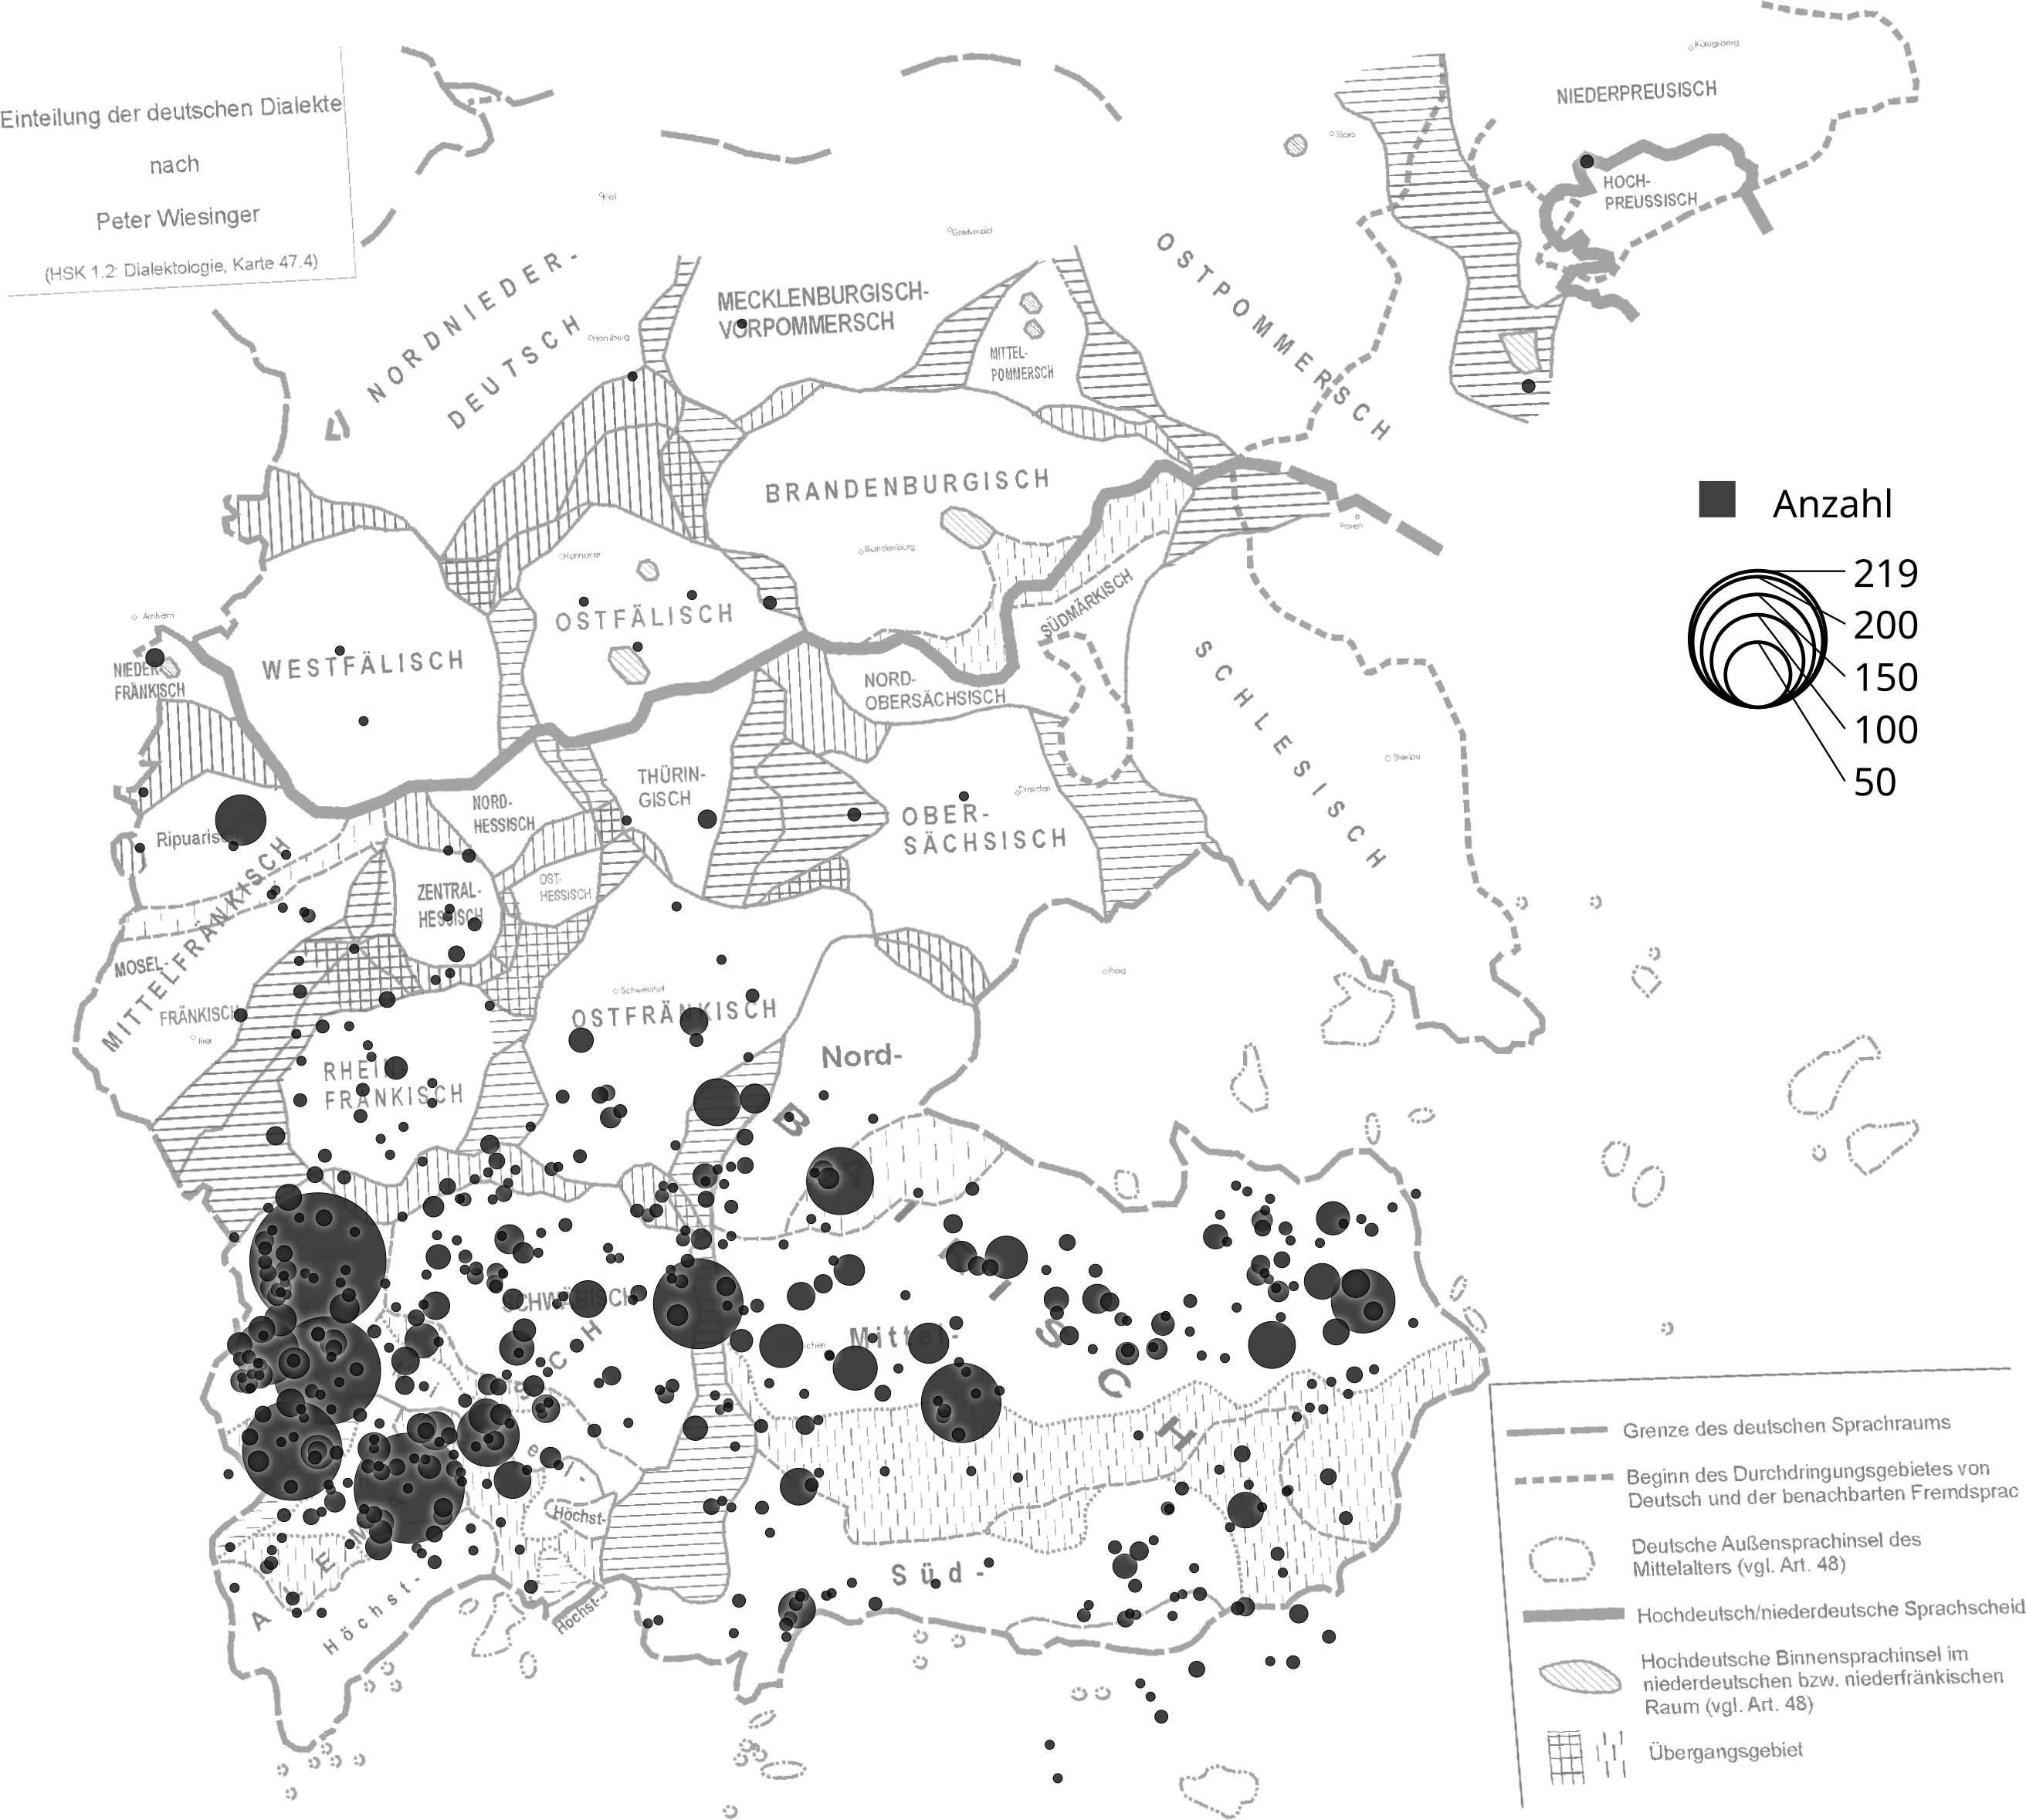
\includegraphics[
	width=\linewidth,
	keepaspectratio
]{./figures/2022-03-03_deedsperplace.png}
\caption{Urkunden pro eindeutigem \CAO{}-Ausstellungsort
	(Hintergrundkarte: \cite{wiesinger1983:rede})
}
\label{fig:cao_urkorte}
\end{figure}

Das \CAO{} hat den Anspruch, die gesamte Urkundenüberlieferung des
13.~Jahrhunderts zu versammeln. Auch wenn es eine \q{Dunkelziffer} an Urkunden
gibt, die nicht in die Sammlung aufgenommen wurden, wird die Zunahme an
deutschsprachigen Urkunden in \tabref{tab:urkstat} deutlich; der Großteil der
Urkunden im \CAO{} entfällt auf die letzten beiden Jahrzehnte. Während
der westoberdeutsche Sprachraum zunächst bei der Ausstellung deutschsprachiger
Urkunden führt, holt der ostoberdeutsche ab den 1280er Jahren massiv auf und
übertrifft den westoberdeutschen am Ende der Dekade schließlich um etwa
4,6\,\% \autocite[46--47]{ganslmayer2012}.%
%
	\footnote{\citet[47]{ganslmayer2012} weist im Abschnitt von 1290--1299 für
		das Alemannisch-Schwäbische 38,79\,\% der im \CAO{}
		enthaltenen Urkunden aus sowie für das Bairische insgesamt 43,4\,\%.
	}

\begin{table}
\centering
\caption{Anzahl der Urkunden im \CAO{} pro Jahrzehnt
\autocite[40]{ganslmayer2012}}
\begin{tabularx}{\textwidth}{l C C C C}
\lsptoprule
%
	& \textbf{bis 1279}
	& \textbf{1280--89}
	& \textbf{1290--99}
	& \textbf{Summe}
	\\

\midrule

Anzahl insgesamt
	& 621
	& 1.095
	& 2.901
	& 4.617
	\\

davon deutschsprachig
	& 585
	& 1.007
	& 2.697
	& 4.289
	\\

\lspbottomrule
\end{tabularx}
\label{tab:urkstat}
\end{table}

Insgesamt lässt sich festhalten, dass die Urkunden des \CAO{} für linguistische
Fragestellungen eine Reihe von Vorteilen bieten. Zum einen handelt es sich um
Gebrauchsprosa, die im Rahmen von großteils privaten Rechtsgeschäften das
alltägliche Leben der Zeit in vielfältiger Weise berühren. Damit stehen die
Urkundentexte tendenziell näher an der Alltagssprache als literarische Texte,
die besonders in der älteren Grammatikschreibung zum
Mittelhochdeutschen\il{Mittelhochdeutsch} überproportional repräsentiert waren.
Die Urkunden stellen in der Regel das schriftlich festgehaltene Ergebnis
mündlich geführter Verhandlungen dar \autocite[595]{schmidtwiegand1998b}. Zum
anderen ist das \CAO{} für sprachgeschichtliche Untersuchungen gut geeignet, da
größter Wert auf eine zuverlässige Transkription gelegt wurde. Die Urkunden
sind darüber hinaus zumeist datiert und enthalten Informationen, mit denen sie
sich regional zuordnen lassen, was gerade für sprachgeografisch orientierte
Analysen eine ideale Voraussetzung ist \autocite[22]{schulze2011}.

Obwohl bei der vorliegenen Untersuchung nicht sämtliche Urkunden untersucht
wurden (vgl. \sectref{sec:miningcao}), ist das Ortsnetz dicht genug, dass
Raumstrukturen zutage treten. Besonders hervorzuheben ist der Umstand, dass das
insgesamt zirka zwei Millionen Wortformen umfassende Textkorpus (das heißt
einschließlich der Mehrfachausfertigungen und nicht-deutschsprachiger Urkunden)
vollständig elektronisch vorliegt \autocites{gniffkerapp2005}{cao-online} und
damit eine ansehnliche Datenmenge in ihrer ganzen Breite handhabbar wird
\autocite{beckerschallert2021,beckerschallert2022b}.%
%
	\footnote{Zum Vergleich mit anderen elektronischen Korpora zu historischen
	Sprachstufen des Deutschen siehe \citet{dipper2015}.
	\citet[391]{gniffkerapp2005} beziffern den Umfang des \CAO{} mit
	\blockquote{etwa 1,3 Millionen Belegwörtern}, wobei sie sich dabei
	vermutlich nur auf das deutschsprachige Material ohne Doppelausfertigungen
	beziehen.} % (vgl.~\sectref{fn:caowordcount}).}

Nachteilig ist, dass nicht an jedem Ort gleich große Mengen an Urkunden
vorliegen, zumal die Urkunden des \CAO{} lediglich eine Momentaufnahme
größtenteils der letzten zwanzig Jahre des 13.~Jahrhunderts bieten. Darüber
hinaus besteht das Problem, dass sich Schreiberinnen und Schreiber in der Regel
nicht greifen lassen, sodass aus der einzelnen Urkunde heraus nicht deutlich
wird, ob sie genuin ortstypische Sprache reflektiert. Diesen Nachteilen lässt
sich jedoch mit einer Kombination von quantitativer und qualitativer Analyse
begegnen. Da einzelne Belege wenig aussagen, braucht es eine gewisse Masse an
Belegen, um Tendenzen deutlich zu machen.
Zu kleinteiligen Aus\-sagen zur Mundart einzelner Orte wird man über die
Untersuchung der Urkunden nicht gelangen, wohl aber zu Aussagen über das
Verhalten unterschiedlicher Schreibregionen und die Reflexion divergierender
Sprachmerkmale im regionalen Schreibgebrauch.

%%%%%%%%%%%%%%%%%%%%%%%%%%%%%%%%%%%%%%%%%%%%%%%%%%%%%%%%%%%%%%%%%%%%%%%%%%%%%%%

\section{Die \tit{Kaiserchronik}}
\label{sec:materialkc}

Die \tit{Kaiserchronik} (\KC{}) ist eine Reimchronik in deutscher Sprache, die
um die Mitte des 12.~Jahrhunderts vermutlich in Regensburg entstanden ist.%
%
	\footnote{Einen Überblick bietet \citet{nellmann1983}. Zum aktuellen
	Forschungs- und Editionsstand siehe das \tit{ZfdA}-Themenheft zur \KC{}
	\autocite{wolf2019} sowie jüngst die Dissertation von \citet{weis2022}.
	Angaben zur Entstehungszeit und zum Schreibdialekt der jeweiligen
	Textzeugen basieren auf dem derzeit noch unveröffentlichten Katalog von
	\citet{wolf:kckat}, siehe auch \citeurl{kcdigital}\nocite{kcdigital}
	sowie den \citet[s.\,v.~\textit{\tit{Kaiserchronik}}]{hsc} mit den dort
	angegebenen Quellen.}
%
Sie ist anonym überliefert und auch die Frage nach ihrem Auftraggeber ist
ungeklärt. \citet[92]{wolf2008} bescheinigt der \KC{}
\blockquote{ein Formen-, Sprach- und Normeninventar, das für die
volks\-sprachig-höfische Literatur des Spätmittelalters zu einem Grundmuster
wird}.

Der Text ist in bislang fünfzig bekannten Textzeugen zwischen dem letzten
Viertel des 12.~Jahrhunderts (A1) und dem späten 16.~Jahrhundert (T)
überliefert \autocite[39, 57]{wolf:kckat}; der Überlieferungsschwerpunkt fällt
in das 13.~Jahrhundert
\autocites[vgl.][s.\,v.~\textit{\tit{Kaiserchronik}}]{hsc}{kcdigital}. Im Lauf
ihrer etwa vierhundertjährigen Überlieferungsgeschichte hat die \KC{} zwei
Überarbeitungen erfahren: um ca.~1200 (\q{Rezension~B}) und um ca.~1250
(\q{Rezension~C}) \autocites{wolf2008}. \citet[369]{gaertner1995} zufolge
unterscheiden sich die Rezensionen B und C so stark von der ältesten Fassung
(\q{Rezension~A}), dass sie jeweils neue Werke darstellen;
\citet[142]{chincaetal2019a} sprechen mit \citet{bumkepeters2005} in diesem
Zusammenhang von \q{Retextualisierung}.

Die \KC{} handelt ihrer eigenen Aussage nach \norm{von den bâbesen unt von den
chunigen, baidiu guoten unt ubelen} `von den Päpsten und von den Königen,
sowohl guten als auch schlechten' (\KC: V.~19--20; \cite[79]{schroeder1895}).
Die einzelnen Episoden zu den jeweiligen Kaisern von Cäsar bis Konrad~III.\
(A/B), beziehungsweise je nach Fortsetzung Friedrich~II. oder Rudolf~I. (C),
verselbstständigen sich bisweilen zu eigenen Erzählungen und haben eher den
Charakter eines Fürstenspiegels als den eines strikt historiografischen
Abrisses, zumal die historische Reihenfolge der Kaiser nicht immer eingehalten
wird, zwei römische Kaiser hinzugedichtet werden und die Angaben zu den
Regierungszeiten der jeweiligen Kaiser am Ende jeder Episode willkürlich sind
\autocite[954--960]{nellmann1983}. Stattdessen soll
\blockcquote[957]{nellmann1983}{\textins*{m}öglichst jede Kaisergeschichte
\textelp{} den \textquote{heilsgeschichtlichen Kampf der guten und der bösen
Mächte} \textelp{} zur Anschauung bringen}.

Erste Ausgaben des Volltexts der \KC{} erfolgten von \citet{massmann:kukb}
sowie von \citet{diemer1849} nach der damals gerade neu entdeckten Vorauer
Handschrift (A1). Die bisher maßgebliche Edition ist die von
\citet{schroeder1895}. Die genannten drei Editionen geben alle den Text
der Rezension~A wieder, \citeauthor{massmann:kukb} bietet ausschnittsweise auch
Teile von B und C.%
%
	\footnote{Ein kritisches Resümee zu \citeauthor{massmann:kukb}s
		Editionstätigkeit zieht \citet{wolf2023}, in Bezug auf die
		\KC{} siehe dort, \notecite[\pno~122--132]{wolf2023}.
		\citeauthor{massmann:kukb}s Edition der \KC{} beruht auf der
		Heidelberger A-Handschrift (H), deren Text er mäßig normalisiert im
		Grunde als Leithandschrift bietet, allerdings ermangelt sein Text
		bisweilen philologischer Stringenz und ist damit nicht unproblematisch
		\autocite[125--126]{wolf2023}. Obwohl \citeauthor{massmann:kukb} nach
		\posscite[131--132]{wolf2023} Urteil zugute zu halten ist, dass in den
		\textquote{Beigabenpaketen} auch zur \KC{}-Edition durchaus
		viel Nützliches an Meta-, Inter- und Paralleltexten enthalten ist,
		zeichnen sich diese Beigaben durch \textquote{eine überbordende Fülle
		gepaart mit einer chaotisch anmutenden Un-Ordnung} negativ aus,
		\textcquote[131]{wolf2023}{und zwar insbesondere dann, wenn Fakten und
		Phantasie (bei Maßmann nicht selten) zusammenfließen}, vor allem im
		Sinne seiner vom Nationalismus geprägten politisch-historischen
		Interessen.%
	}
%
Die Edition von \citeauthor{schroeder1895} ist zwar insofern normalisiert, als
Schreibweisen vereinheitlicht sowie Vokal\-längen und moderne Interpunktion
eingefügt wurden. Sie verfolgt im Großen und Ganzen aber das
Leit\-handschriften\-prinzip auf der Grundlage von A1. \citeauthor{diemer1849}
stellt einen diplomatischen Abdruck zur Verfügung. Eine textkritische Ausgabe,
die die Texte der Rezensionen~B und C als gleichberechtigt neben A behandelt,
ist bisher ein Desiderat.

Mit dem Projekt zur Neuedition der \KC{} in Form einer synoptischen Ausgabe
wird die Einlösung dieses Desiderats unter der Leitung von Mark Chinca, Helen
Hunter, Christopher Young (Cambridge) und Jürgen Wolf (Marburg) seit 2012
verfolgt \autocite{chincaetal2019b}. Zu diesem Zweck wurden sämtliche bekannten
und noch existenten Textzeugen auf Basis von Digitalfotos der
Handschriften\-originale diplomatisch transkribiert. Farb\-digitalisate und
XML-ko\-dier\-te Transkriptionen sind über die Universität Heidelberg
öffentlich zugänglich.%
%
	\footnote{Siehe \citeurl{kcdigital}\nocite{kcdigital}.}
%
\citet[287]{chincaetal2019b} betonen, dass mit der digitalen Edition der
\KC{} \blockquote{Sprachhistoriker \textelp{} die Möglichkeit \textins*{haben},
Vorgänge der dia\-topischen und dia\-chronischen Mikrovarianz zu beobachten,
die im textkritischen Apparat normalen Formats sonst verlorengingen}.

Die einzelnen Textzeugen sind regional verhältnismäßig breit gestreut, haben
allerdings ihren Überlieferungsschwerpunkt im Ostoberdeutschen, wie
\figref{fig:kc_geospac_rough_12}--\ref{fig:kc_geospac_rough_15} deutlich machen
(\cite[vgl.~auch][]{klein1988} für die Rezension~A).%
%
	\footnote{Anders als bei den Urkunden kann für die jeweiligen
		\KC{}-Textzeugen in der Regel kein mehr oder weniger exakter
		Entstehungsort ermittelt werden, daher dienen die Markierungen auf der
		Karte lediglich der Übersicht. Maßgeblich als Angaben zur
		sprachräumlichen Einordnung sind die Beschriftungen
		\autocite[vgl.][]{wolf:kckat}.}
%
Ähnlich wie bei den Urkunden des \CAO{} liegt eine Textsammlung
sozusagen \q{aus einem Guss} vor, da alle enthaltenen Texte dem gleichen
literarischen Werk zugeordnet sind. Ein fundamentaler Unterschied zu den
Urkunden liegt in der Art und Weise der Tradierung des Großteils
mittelalterlicher Texte: \blockquote[{\cites[1310]{wegera2000}[siehe
auch][262--263]{fleischer2019}}]{In der Regel haben wir es mit einer längeren
Text- und Rezeptionsgeschichte, also mit Abschriften und Abschriften von
Abschriften zu tun. Es muß deshalb mit einer erheblichen regional bedingten
Interferenz und mit einer zeitlichen Verzerrung des Sprachstandes gerechnet
werden (Stichwort: Vorlagenproblematik).}

\begin{figure}
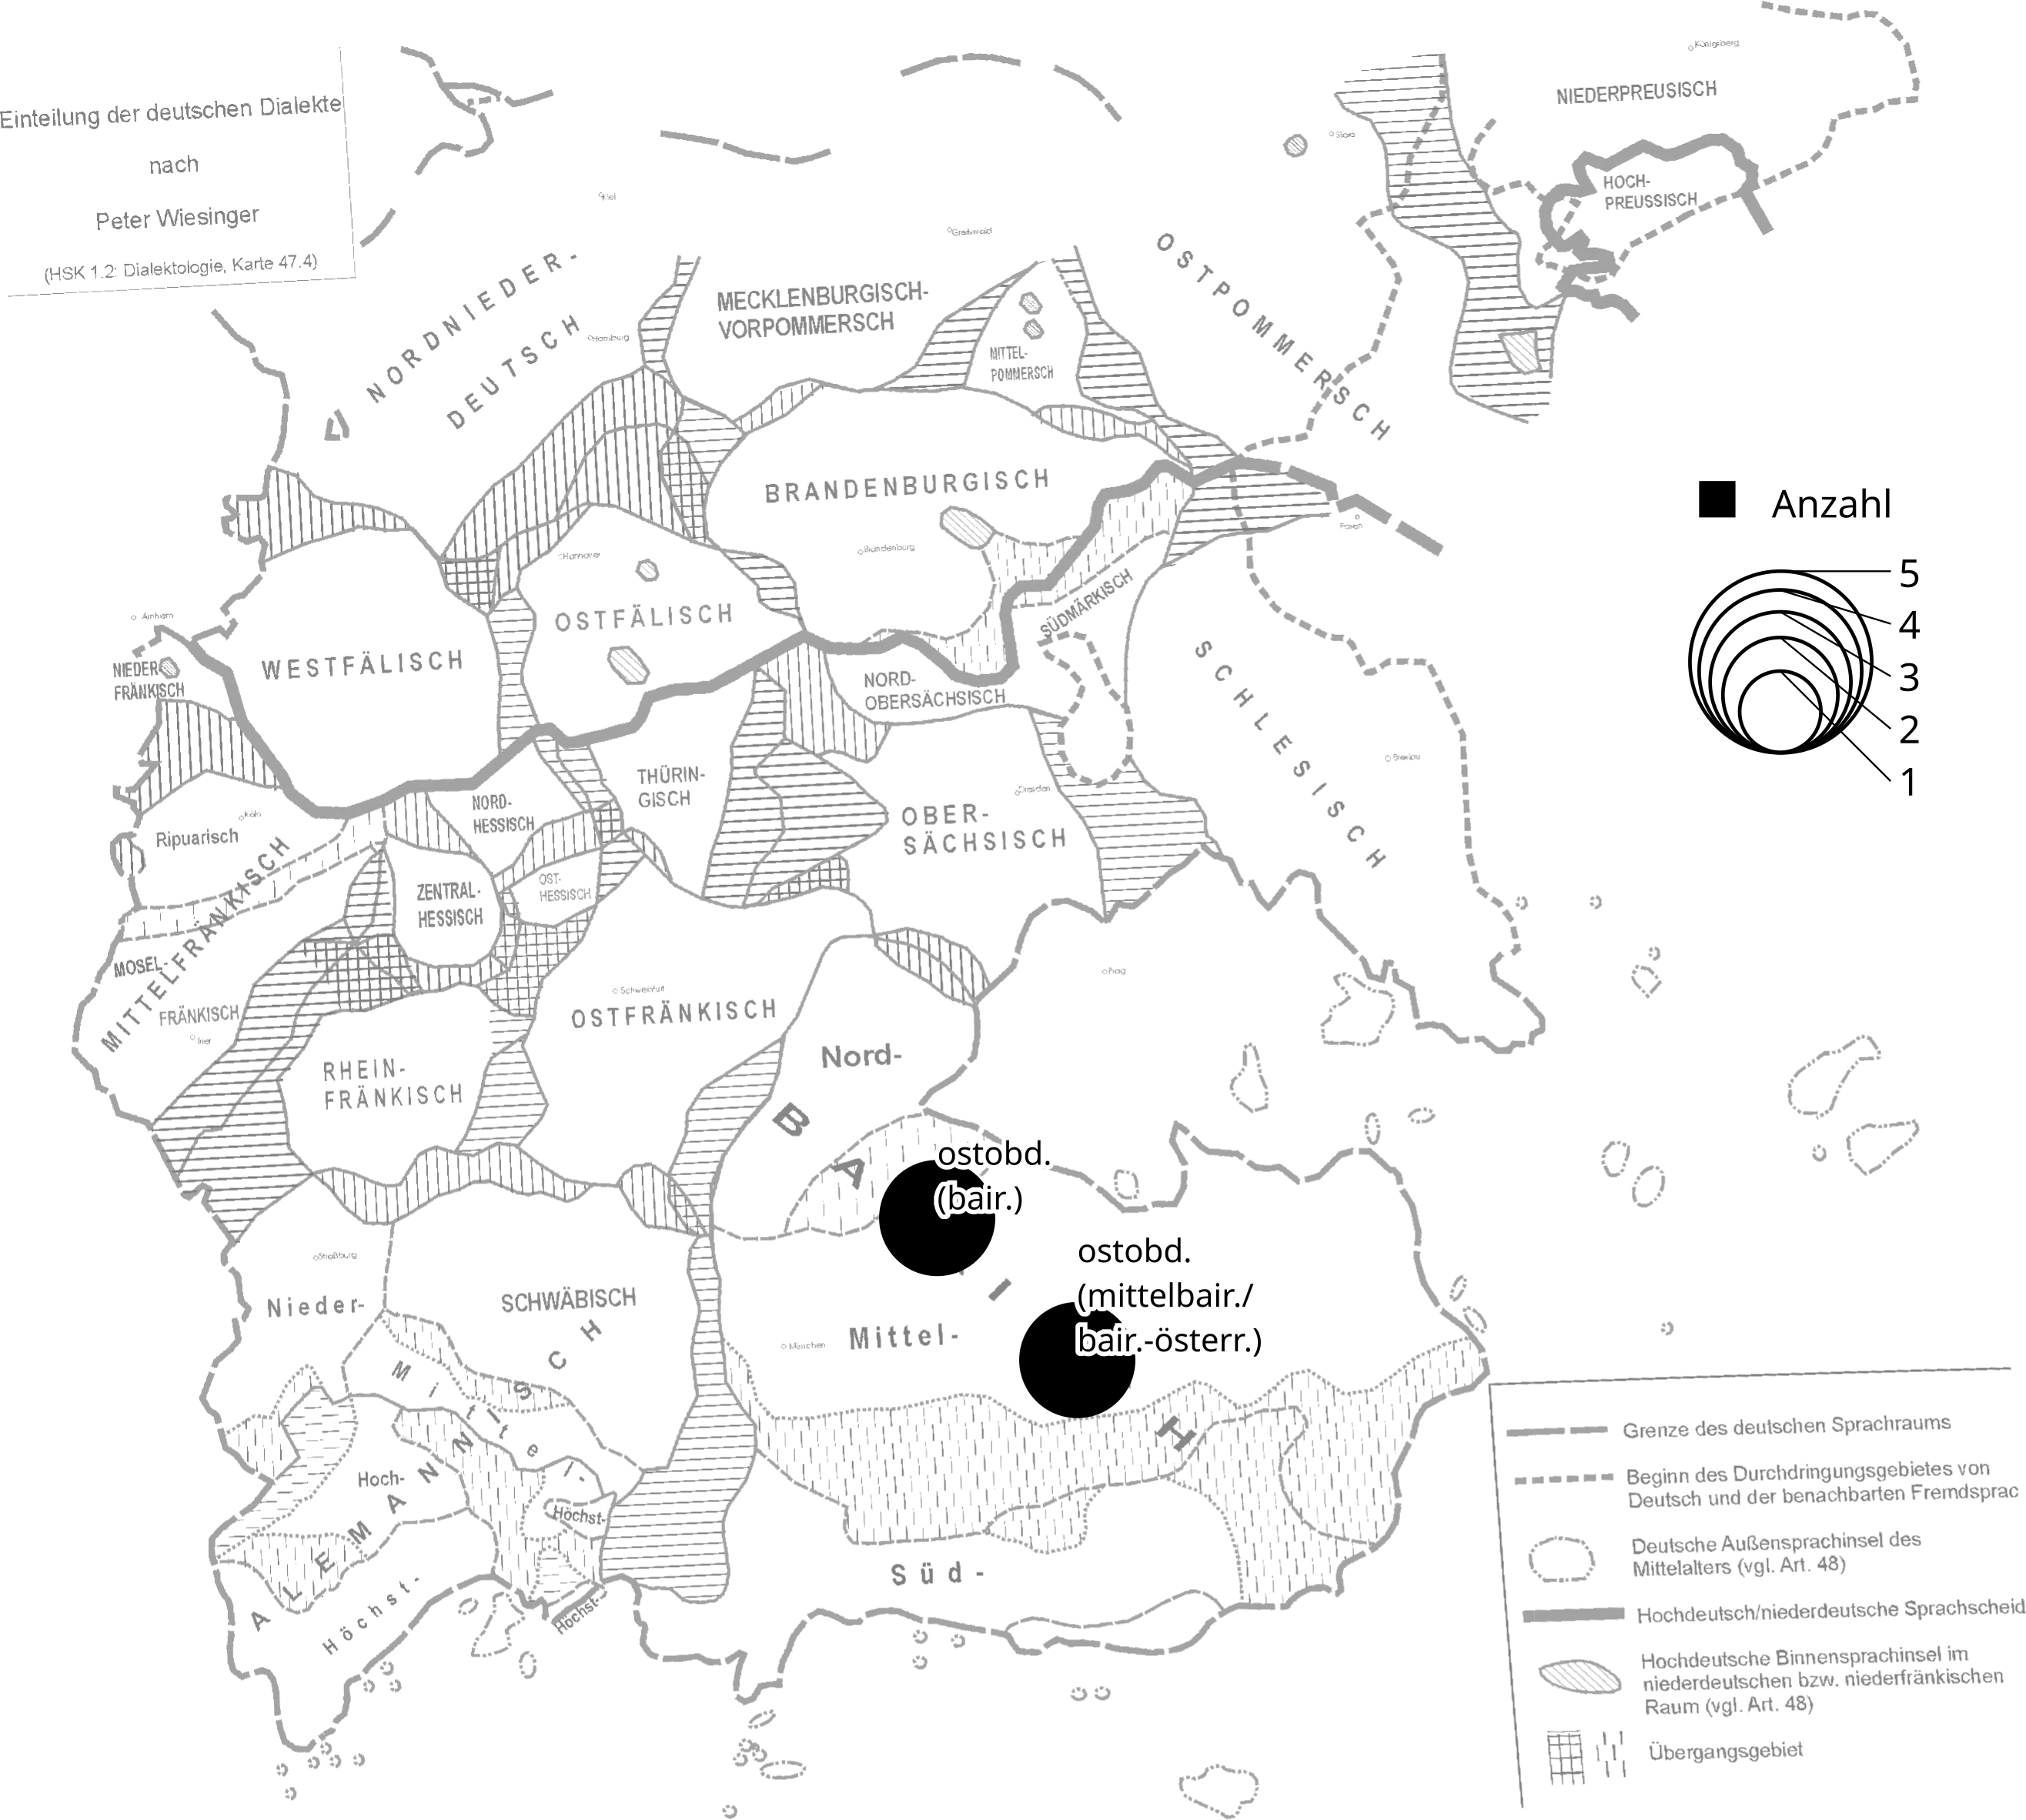
\includegraphics[
	width=\linewidth,
	keepaspectratio
]{./figures/2021-12-30_kc_geospac_rough_c12.png}
\caption%
	{Grobe räumliche und zeitliche Verteilung der \KC{}-Text\-zeugen (12.~Jh.;
	Hintergrundkarte: \cite{wiesinger1983:rede})
	}
\label{fig:kc_geospac_rough_12}
\end{figure}

\begin{figure}
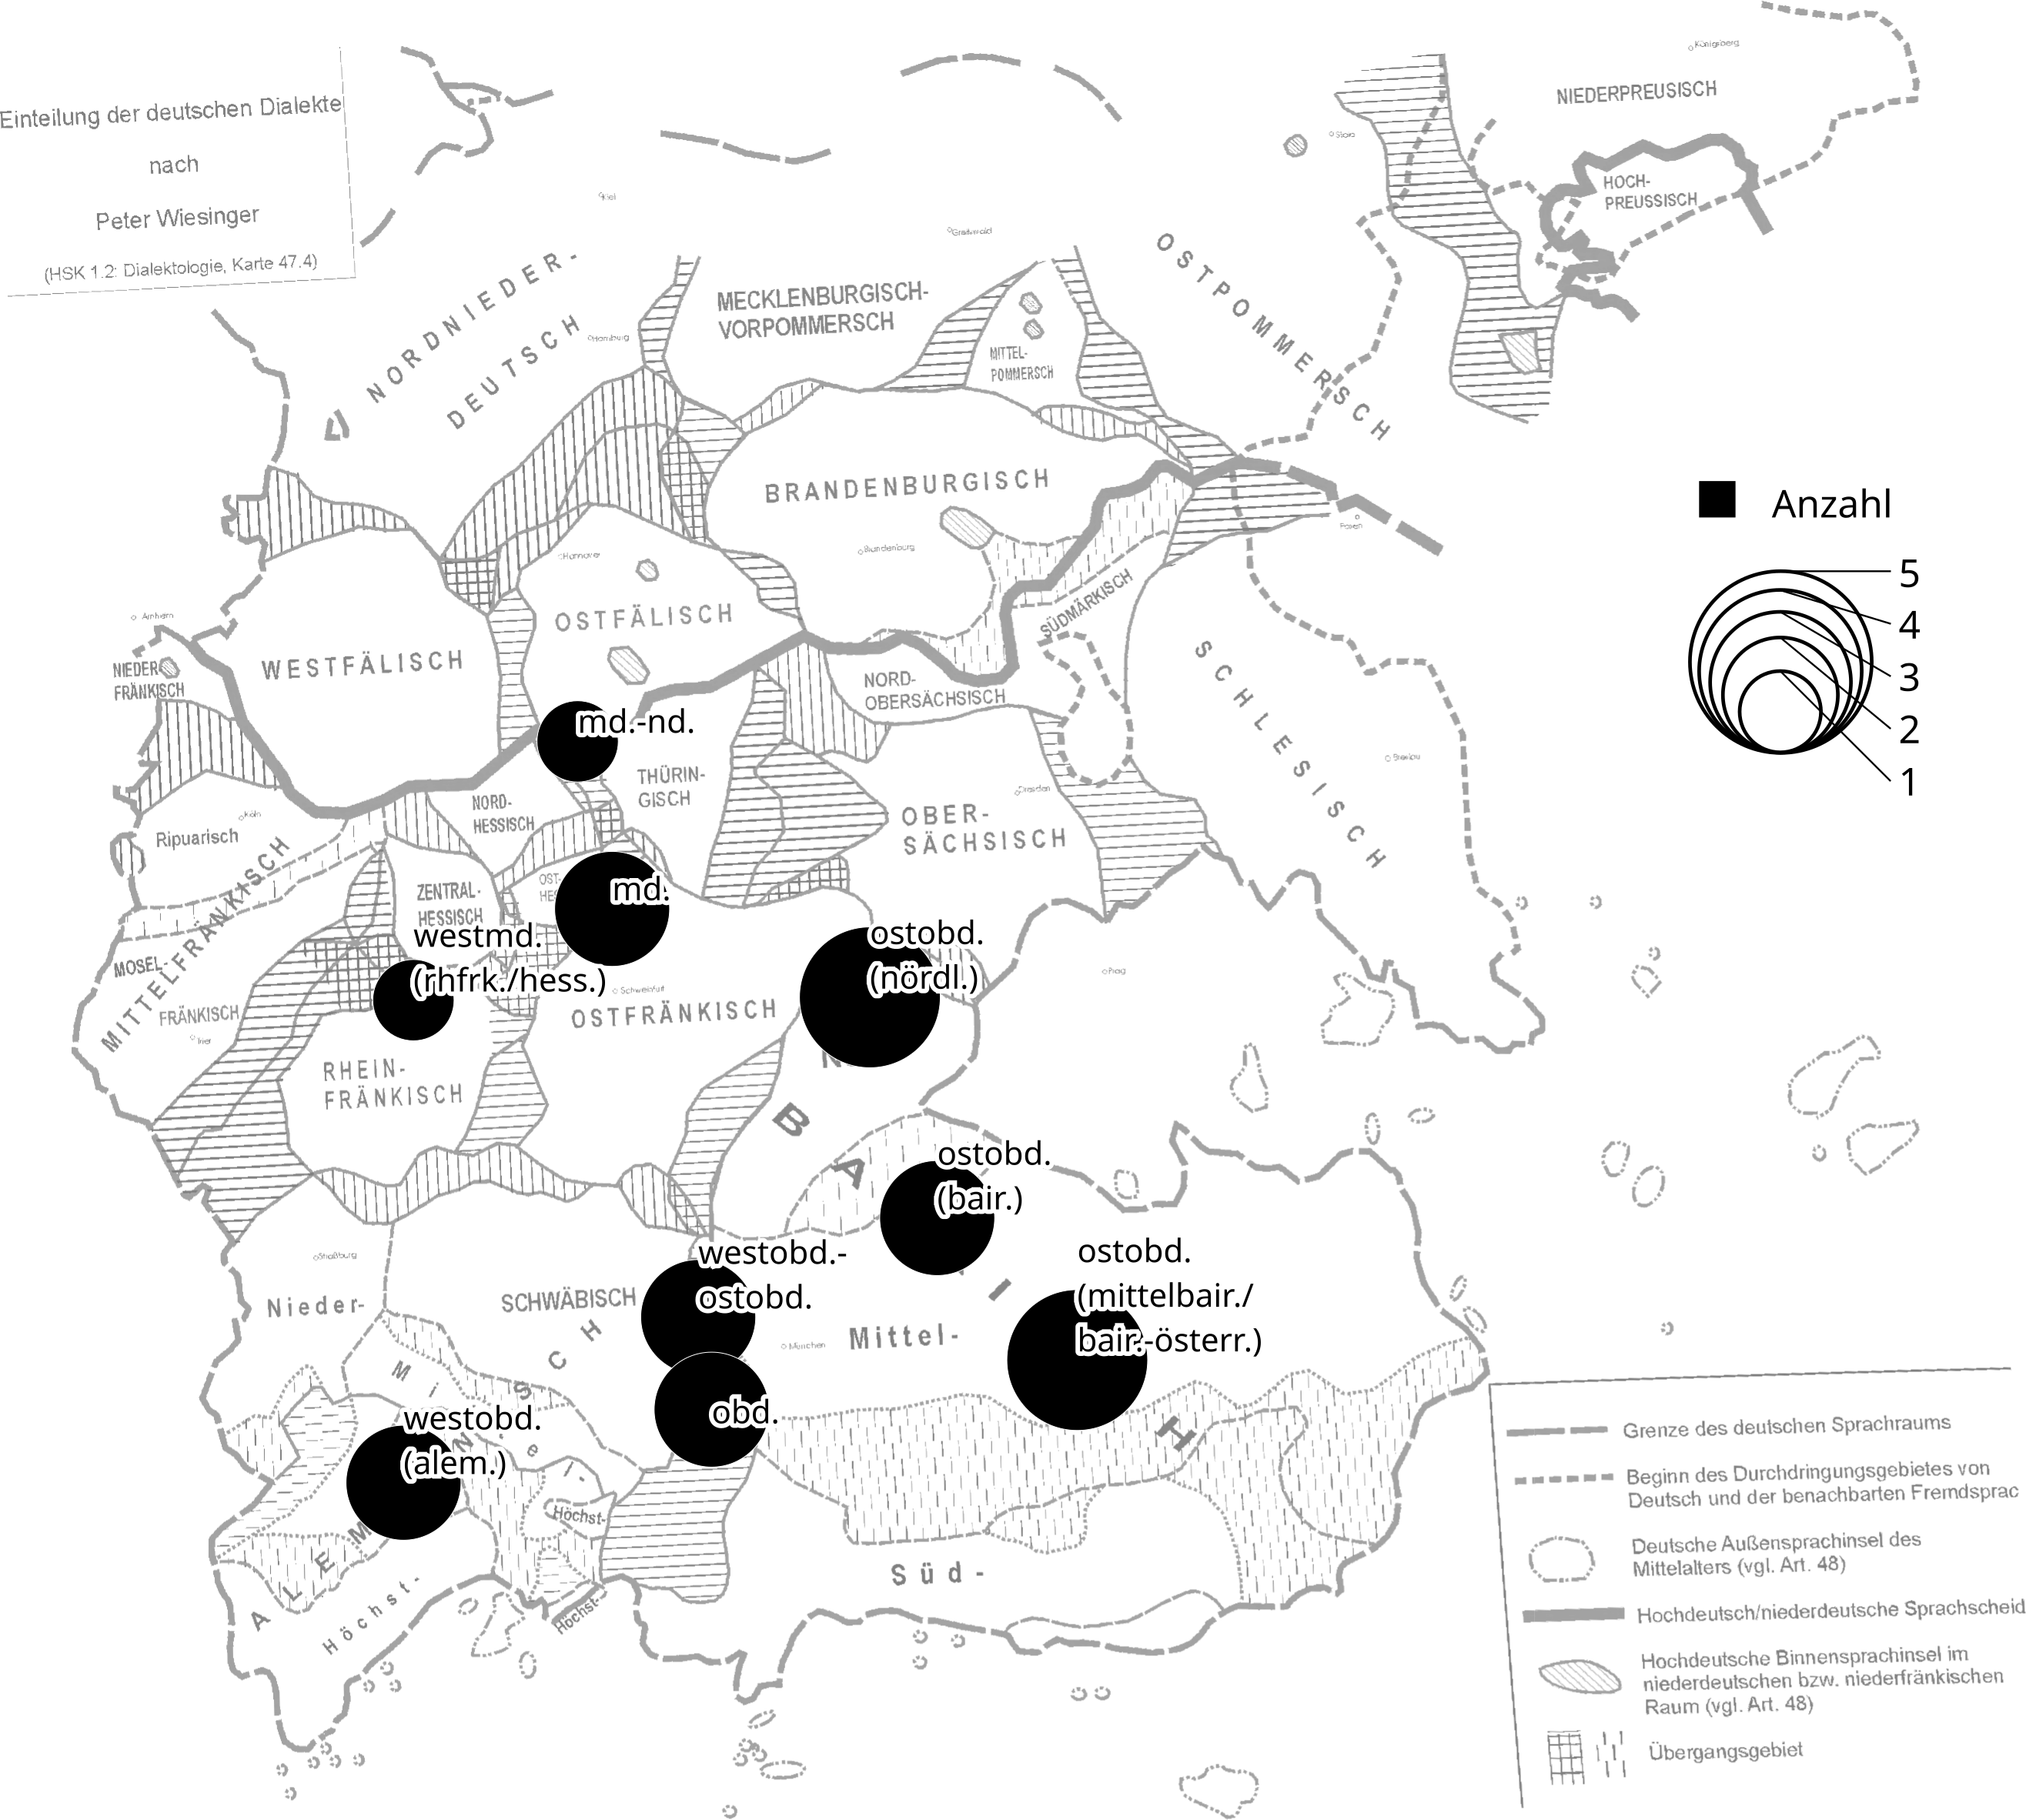
\includegraphics[
	width=\linewidth,
	keepaspectratio
]{./figures/2021-12-30_kc_geospac_rough_c13.png}
\caption%
	{Grobe räumliche und zeitliche Verteilung der \KC{}-Text\-zeugen (13.~Jh.;
	Hintergrundkarte: \cite{wiesinger1983:rede})}
\label{fig:kc_geospac_rough_13}
\end{figure}

\begin{figure}
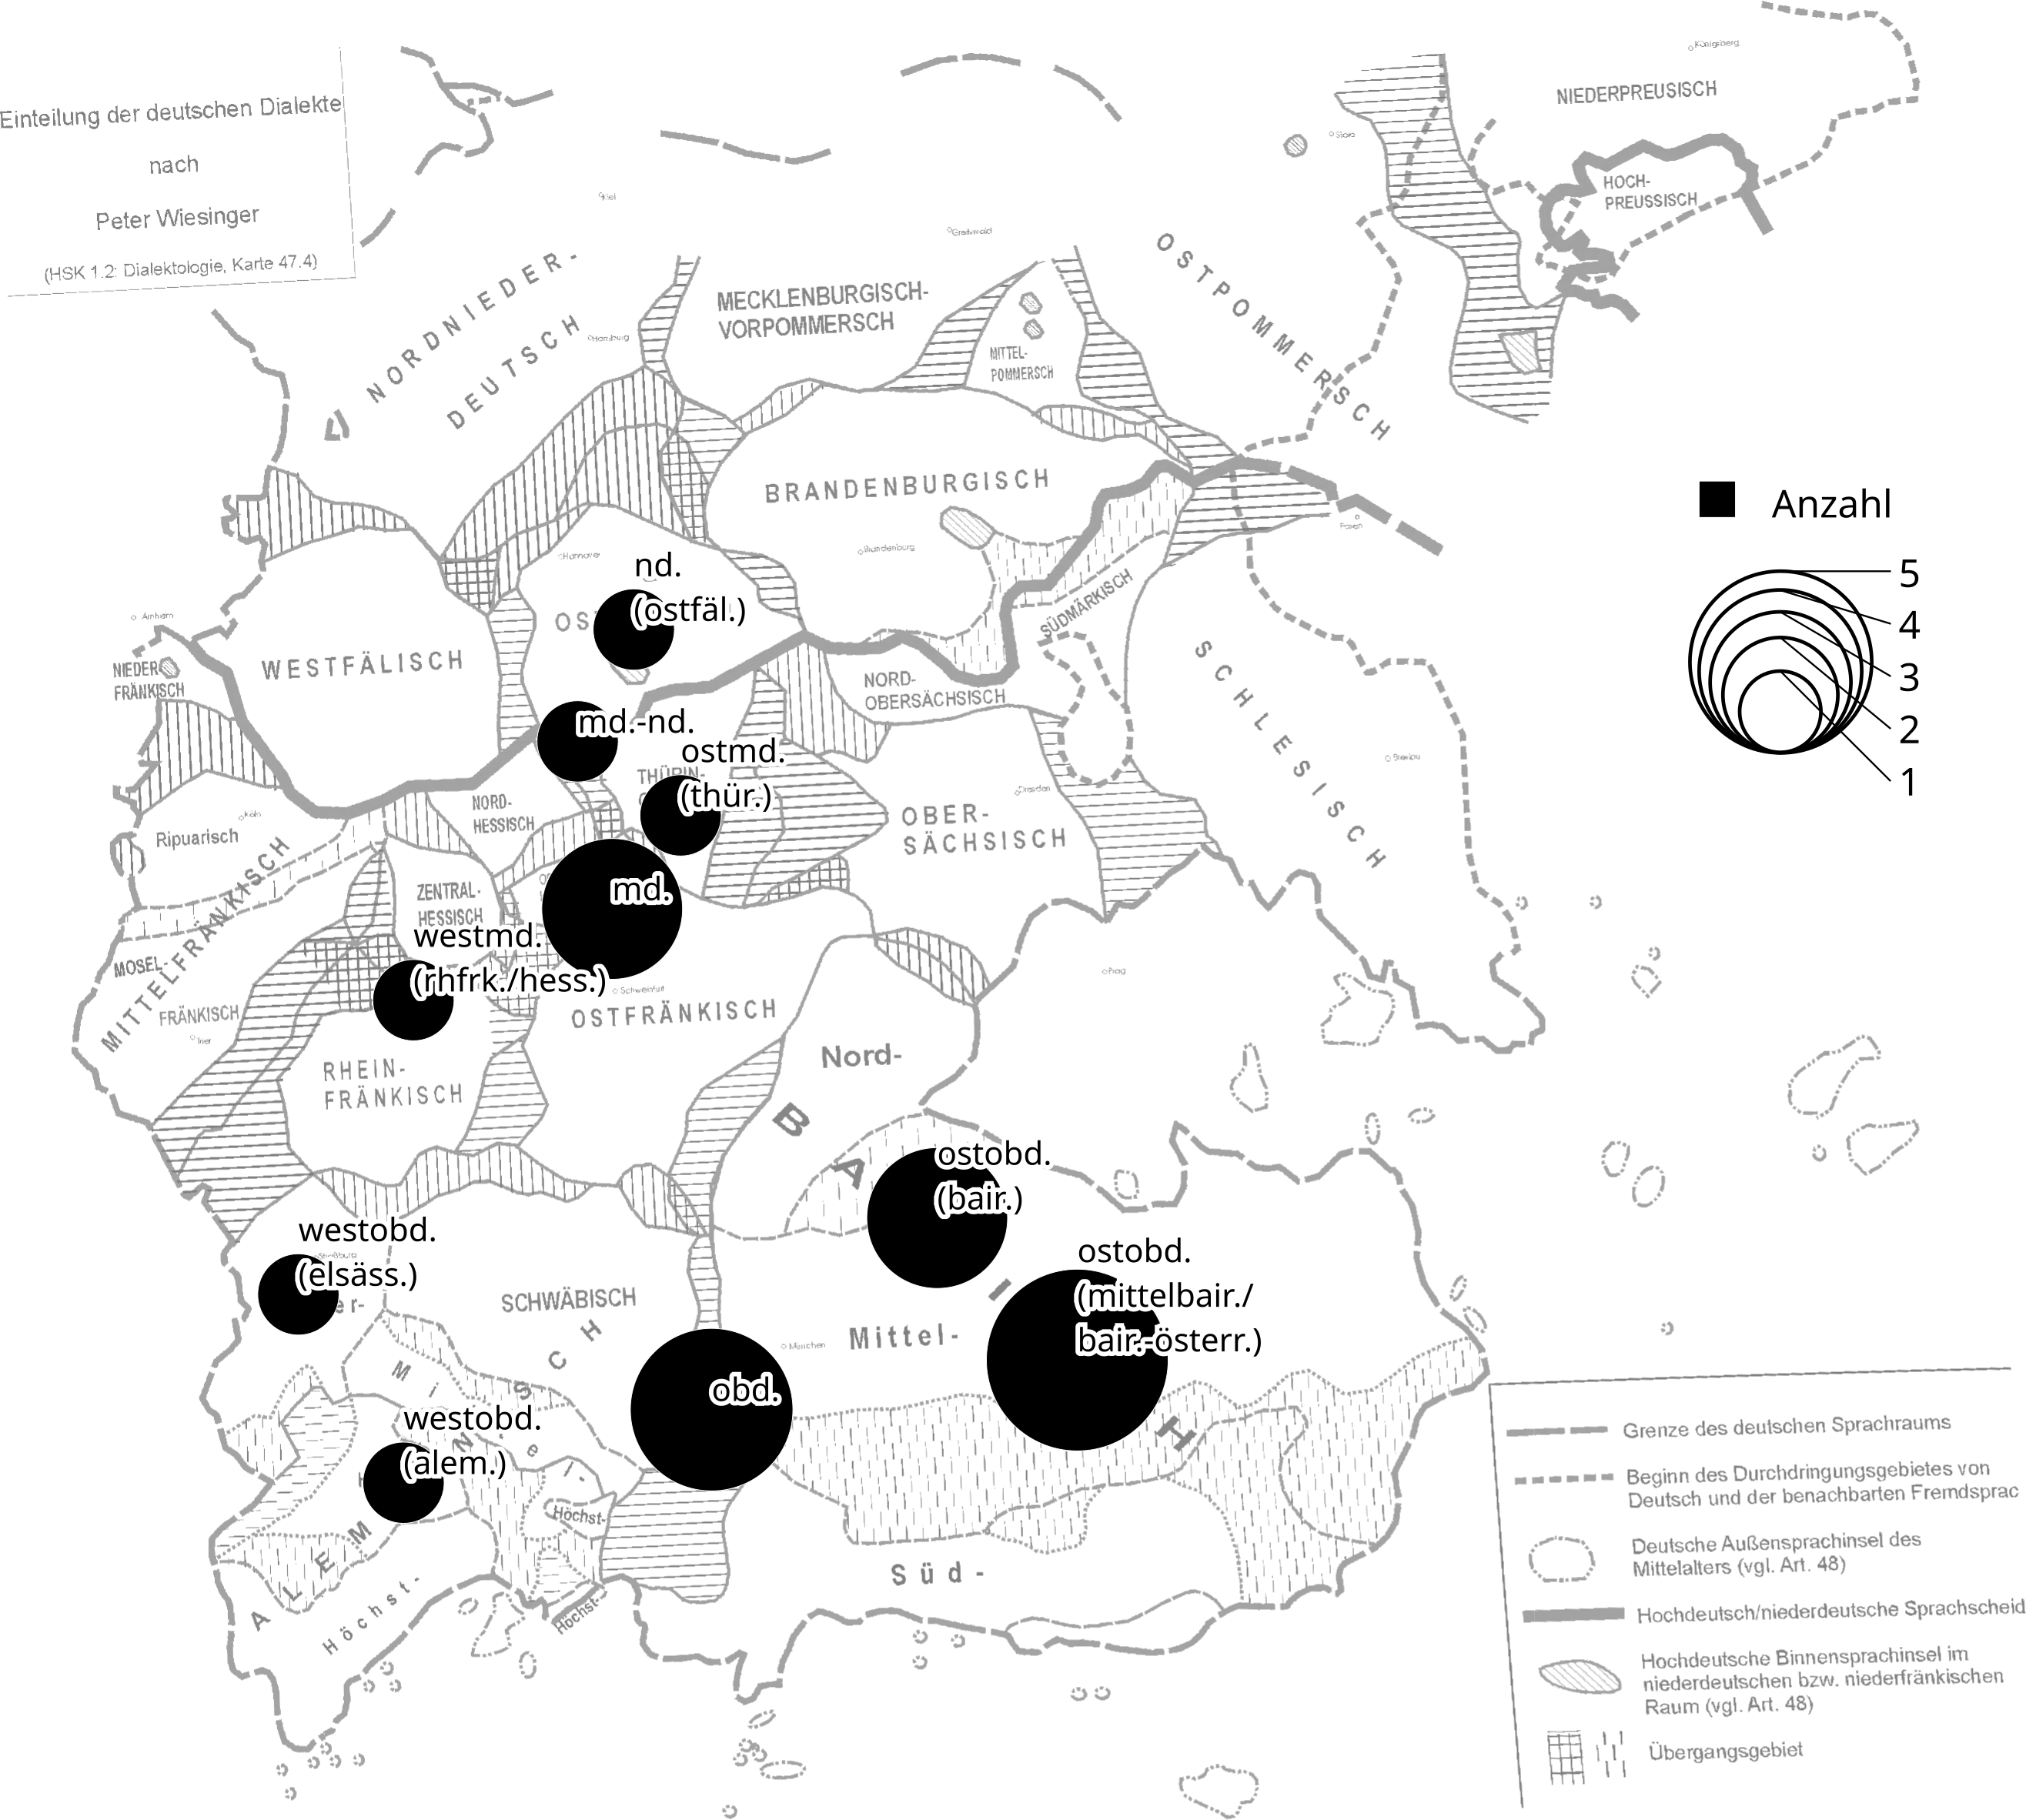
\includegraphics[
	width=\linewidth,
	keepaspectratio
]{./figures/2021-12-30_kc_geospac_rough_c14.png}
\caption%
	{Grobe räumliche und zeitliche Verteilung der \KC{}-Text\-zeugen (14.~Jh.;
	Hintergrundkarte: \cite{wiesinger1983:rede})}
\label{fig:kc_geospac_rough_14}
\end{figure}

\begin{figure}
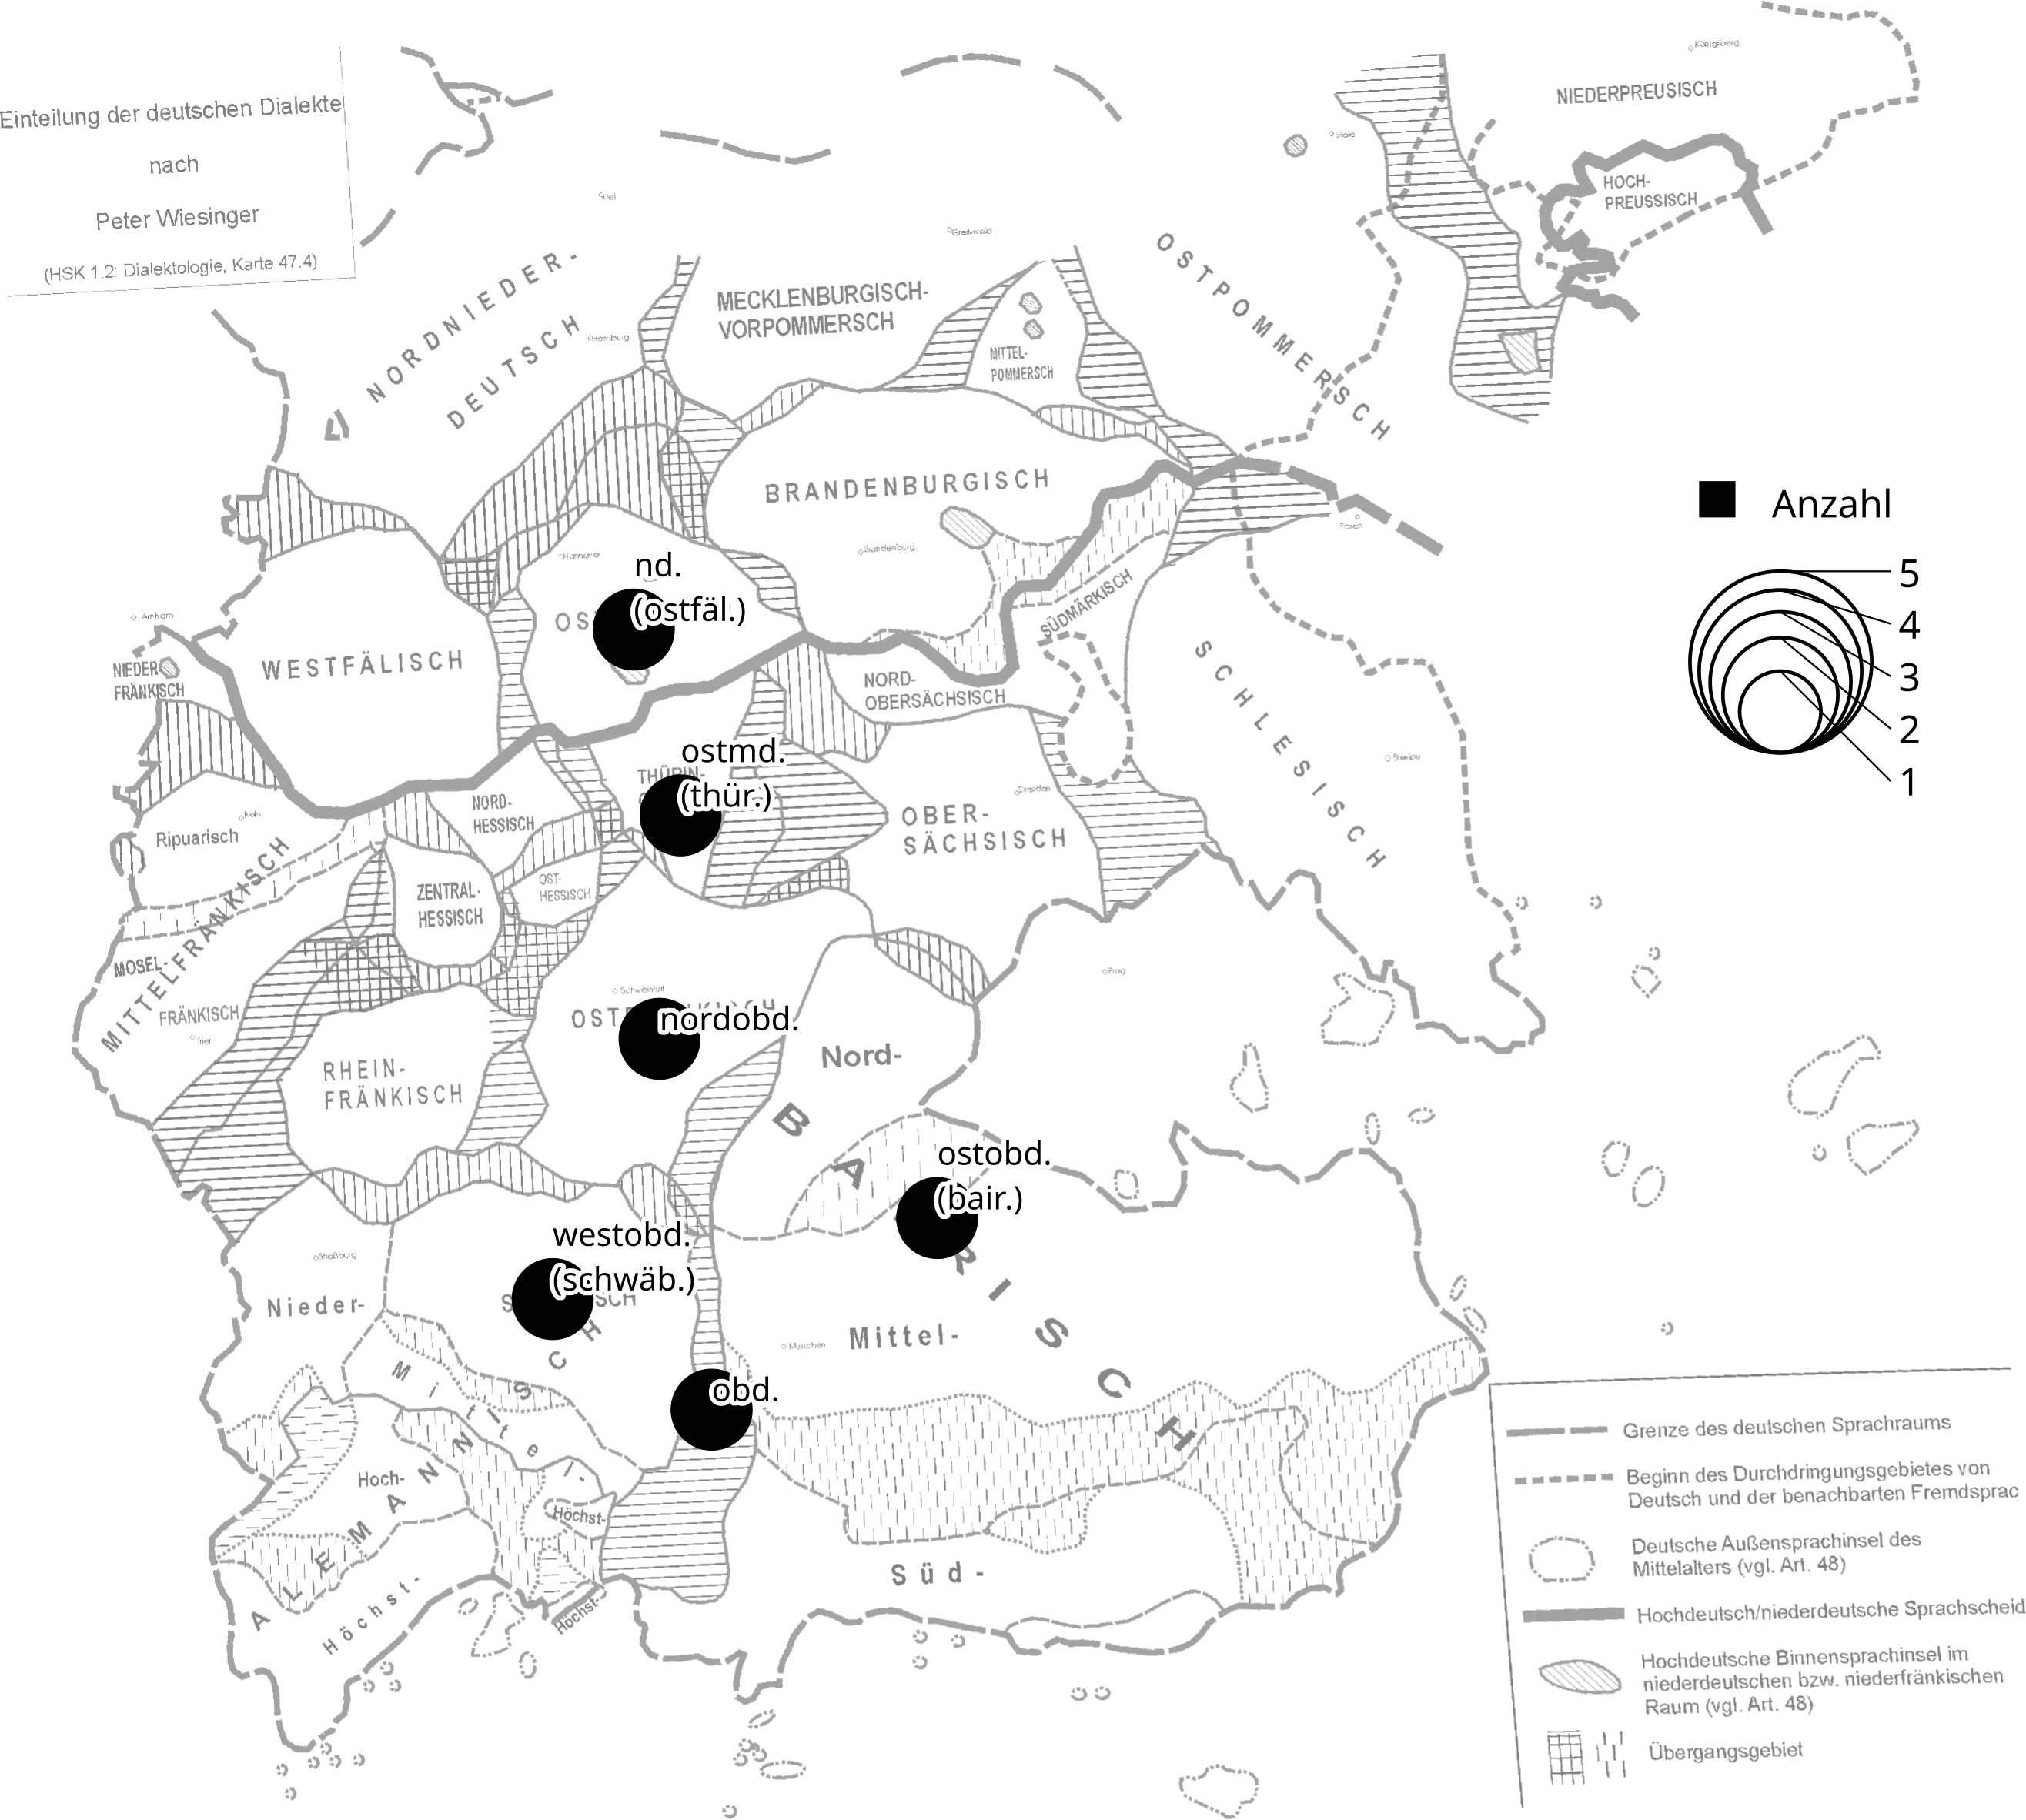
\includegraphics[
	width=\linewidth,
	keepaspectratio
]{./figures/2021-12-30_kc_geospac_rough_c15.png}
\caption%
	{Grobe räumliche und zeitliche Verteilung der \KC{}-Text\-zeugen (15.~Jh.;
	Hintergrundkarte: \cite{wiesinger1983:rede})}
\label{fig:kc_geospac_rough_15}
\end{figure}

Die handschriftliche Überlieferung der \KC{} bietet daher ein entscheidendes
Merkmal der geschäftsmäßigen Schriftlichkeit (Urkunden, Urbare) oftmals gerade
nicht: Autornähe. Des Weiteren sind die Handschriften der
\KC{} im Gegensatz zu den Urkunden des \CAO{} weder exakt datiert
noch einigermaßen genau lokalisierbar. Aufgrund der von
\citet[1310]{wegera2000} angesprochenen \q{Vorlagenproblematik} muss außerdem
tendenziell davon ausgegangen werden, dass Dialekt\-mischungen eher die Regel
als die Ausnahme darstellen. Der Vergleich der Daten aus der Auswertung der
\KC{} mit denen der \CAO{}-Auswertung verspricht also besonders
valide Ergebnisse, insofern sich mit Hilfe der Urkunden regionale Merkmale von
Schreibdialekten verorten lassen, trotz der grundsätzlichen
Schreiberproblematik und der Einschränkung, dass die Urkunden lediglich eine
Momentaufnahme der geschriebenen Geschäftssprache des späten 13.~Jahrhunderts
darstellen.

Bezüglich der regionalen Variation von Schreibdialekten weist \citet{solms2014}
darauf hin, \blockcquote[132]{solms2014}{dass es die überaus große
Zersplitterung des Sprachgebietes, wie sie die Dialektgeographie des
19.~Jahrhunderts erwiesen hat, in der Schreibsprachlichkeit des 11.\ bis
14.~Jahrhunderts noch nicht gegeben hat}. Andererseits lässt sich fragen,
inwiefern die angesprochene Zersplitterung ein Artefakt der Erhebungsmethode
etwa von Sprachatlanten darstellt. Dialektgeografische Karten bilden nie die
Gesamtheit der Sprecherinnen und Sprecher mit sämtlichen Variations\-ebenen ab,
sondern unterliegen notwendigerweise Abstraktionen und Vereinfachungen, auch
durch die Auswahl der Informantinnen und Informanten. Diese
Komplexitätsreduktion produziert unter Umständen scharfe Grenzen, wo Übergänge
in der Realität fließend sind.

\chapter{Methodik der Datenerhebung}
\label{ch:methoden}

\section%
	{Datenerhebung aus dem \tit{Corpus der altdeutschen Originalurkunden}}
\label{sec:miningcao}

Die Daten für die Teilauswertung zum \tit{Corpus der altdeutschen
Originalurkunden} (\CAO) wurden aus der in
\textcites[207]{beckerschallert2021}[155--158]{beckerschallert2022b}
beschriebenen Datenbank exzerpiert. Grundlage dafür bildet die digitalisierte
Fassung des \CAO{} \autocites{cao-online}[vgl.~dazu][]{gniffkerapp2005}
inklusive der von \citeauthor{beckerschallert2022b} vorgenommenen Zuordnung von
Ortskoordinaten. Das \CAO{} umfasst insgesamt etwa zwei Millionen Wortformen
inklusive Mehrfachausfertigungen und nicht-deutschsprachiger Urkunden. Pro
Urkunde liegen damit durchschnittlich 453 Wortformen vor, die
Standardabweichung beträgt 500 Wortformen.

Wie in \sectref{sec:materialcao} bezüglich der Text\-treue des \CAO{} beschrieben,
gehe ich davon aus, dass die in der Edition gebotenen Transkriptionen für die
Zwecke dieser Untersuchung hinreichend fehlerfrei sind. Bei der Belegsammlung
wurden nur solche Urkunden berücksichtigt, die eine eindeutige Jahresangabe
besitzen und die laut der Zuordung im Schreibortverzeichnis von
\citet{cao-online} einem einzigen Ausstellungsort zugeordnet sind. Bei der
näheren Beschäftigung mit dem Material hat sich gezeigt, dass der Zeitfaktor
weniger ausschlaggebend ist, da ohnehin die meisten Textstücke im \CAO{} aus
der Zeit zwischen 1280 und 1299 stammen (vgl.~\tabref{tab:urkstat}).

Bezüglich des Orts sollen aber nur Ausstellungs\-kontexte mit möglichst
kleinräumigem Bezug erfasst werden, um Urkundentexte mit überregionaler Geltung
und gegebenenfalls damit einhergehender Vermeidung von Regionalismen nach
Möglichkeit auszuschließen. Implizit lehnen sich diese Kriterien an die in
\citet[41--42]{ganslmayer2012} diskutierten an, wobei der Faktor \q{Text} in
Bezug auf Parallelausfertigungen und zeitferne Abschriften ignoriert wurde.
Wenn durch die in \citet[155--158]{beckerschallert2022b} geschilderten
Ausschlusskriterien lediglich etwa 50\,\% des Gesamttextbestands zur Verfügung
stehen, dürften die 8,9\,\% der deutschsprachigen Urkunden, die
\citeauthor{ganslmayer2012} aufgrund des Faktors \q{Text} ausschließt, kaum ins
Gewicht fallen (neben 4.289 deutschsprachigen Urkunden weist
\citet[41]{ganslmayer2012} insgesamt 35 lateinische und 293 niederländische
Urkunden aus). Des Weiteren wurde auf eine Bestimmung des Schreibdialekts jeder
einzelnen ausgewerteten Urkunde im Abgleich mit ihrem angegebenen
Ausstellungsort verzichtet.

Die Suche in der Datenbank geschah mit Hilfe eines regulären Ausdrucks
\autocite[dazu z.\,B.][33--37]{perkuhnetal2012}, der auf Basis der Liste der im
\CAO{} belegten Formen des Lemmas \norm{bėide} formuliert wurde \autocites(mit
allen Deklinationsformen insgesamt ca.~2.050 Belege)[vgl.][166--168]{wmu1}.
\tabref{tab:beidespelcao} listet die belegten grafischen Varianten pro Position
im Wort entsprechend diesem Suchausdruck tabellarisch auf.%
%
	\footnote{Die einzige im \tit{\WMU{}} verzeichnete Form mit
		\lit{-t-} ist \lit{beyte} \autocite[166]{wmu1}: \lit{durch beyte deſ
		vor genanten Hugeſ von Luzelſteyn vn̄ Henriches von Fleckenſteyn}
		`durch beide, des vorgenannten Hugo von Lützelstein und Heinrichs von
		Fleckenstein' \autocites(Nr.~N~674, Straßburg, 1294)[484,18]{cao5}.
		Diese Urkunde war nicht Teil der Auswertung. Formen wie
		\lit{bete} oder \lit{pet} stehen ansonsten für \norm{bęte} `Bitte,
		Gebet' oder stellen Formen von \norm{biten} `bitten' dar.}
%
Bei der Suche nach Zeichenketten wurden die Belegstellen nicht automatisch nach
dem syntaktischen Funktionskontext des jeweiligen Belegs (determinierender
Quantor, Konjunktion) geschieden. Diese Zuordnung geschah manuell in einem
zweiten Schritt.

\begin{table}
\centering
\caption{Im \WMU{} belegte Schreibweisen von mhd.~\norm{bėide/-iu} pro
	Position im Wort}
\begin{tabular}{l l l l}
\lsptoprule

\mc{3}{c}{Stamm}
	& \mc{1}{c}{Flexion}
	\\

\cmidrule(r){1-3}
\cmidrule(l){4-4}

\begin{minipage}{1em}
	b\\
	p
\end{minipage}
	& \begin{minipage}{.25\linewidth}
		ai,
		ay,
		aî,
		aͤ,
		aͥ,
		ee,
		ei,
		ey,
		eî,
		eͤ,
		ie,
		iæ,
		âi,
		æi,
		êi,
		e,
		æ,
		é,
		ê
	\end{minipage}
	& \begin{minipage}{1em}
			d\\
			(t)
	\end{minipage}
	& \begin{minipage}{.25\linewidth}
			eiw,
			iuͦ,
			ivͤ,
			iͤv,
			eu,
			ev,
			ew,
			iu,
			iv,
			iû,
			iͮ,
			uͥ,
			vͥ,
			îv,
			e,
			i,
			j,
			u,
			v,
			ú,
			û,
			Ø
	\end{minipage}
	\\
\lspbottomrule
\end{tabular}
\label{tab:beidespelcao}
\end{table}

\phantomsection
\label{phsec:caohiatus}
Insgesamt wurden 401 Belege zu \norm{bėide}-Targets erfasst, von denen 244 auf
Kontexte mit Quantor entfielen, 157 auf Kontexte mit Konjunktion; 55
Belegstellen wurden aus verschiedenen Gründen ausgeschlossen
(vgl.~\tabref{tab:ausgewcao} und \sectref{sec:urkliste}). Von den 4.289 im
\CAO{} enthaltenen Urkunden und 1.021 zuordenbaren Ausstellungsorten sind in
der Stichprobe 291 Urkunden aus 114 Orten vertreten, von denen 256 Urkunden aus
102 Orten für die Auswertung verwendbar waren.

\begin{table}
\centering
\caption{Zahl der gesammelten und ausgewerteten Belegstellen}
\begin{tabular}{l r r r}
\lsptoprule

%
	& Gesammelt
	& Ausgewertet
	& in \%
	\\

\midrule

% Zahlen retrospektiv überprüft am 01.08.23 an
% data/2022-05-19_beide_cao_controller-target.ods

Quantor
	& 244 % gesamt
	& 219 % ausgewertet
	& 89,8 % in %
	\\

Konjunktion
	& 157 % gesamt
	& 127 % ausgewertet
	& 80,9 % in %
	\\

\midrule

Summe
	& 401 % gesamt
	& 346 % ausgewertet
	& 86,3 % in %
	\\

\lspbottomrule
\end{tabular}
\label{tab:ausgewcao}
\end{table}

Zu allen Kongruenztargets wurden die Controller erfasst -- im Fall von Targets
in unmittelbarer Abhängigkeit von pronominalen Controllern diese sowie die
letzte Nennung der Referenten, auf die sie verweisen (\q{Erstcontroller}). Alle
Controller und Targets wurden anschließend nach ihren formalen und semantischen
Personenmerkmalen annotiert. Außerdem wurde jeweils die Wortart festgehalten
sowie die Flexionsform des Targets mit deren Flexionstyp (\norm{-e}, -Ø,
\norm{-iu}) und ob gegebenenfalls Schwa-Apokope vorliegt. Auch der lineare
Abstand der betreffenden aufeinander bezogenen Wortformen und die Domäne der
Kongruenzbeziehung (gleiche Phrase, gleicher Teilsatz, anderer Satz) wurden
registriert.

Targets, bei denen in Urkunden vom gleichen Ort nach kursorischer Durchsicht
kein Unterschied in der starken Adjektivdeklination zwischen \norm{-e} und
\norm{-iu} im Nom./Akk.~Pl.\ ausgemacht werden konnte, wurden ausgesondert
(vgl.~\sectref{sec:adjdeclcao}). Targets, bei denen der Vokal des Flexionssuffixes
im Hiatus steht und der daher zumindest theoretisch elidierbar ist
\autocites[vgl.][90--91]{askedal1973}[191]{gjelsten1980} wurden gesondert
markiert, wenn auch die Urkundentexte nicht an ein metrisches Schema gebunden
sind.

%%%%%%%%%%%%%%%%%%%%%%%%%%%%%%%%%%%%%%%%%%%%%%%%%%%%%%%%%%%%%%%%%%%%%%%%%%%%%%%

\section{Datenerhebung aus der \tit{Kaiserchronik}}

Die Texte der \tit{Kaiserchronik} (\KC) liegen dank \citetitle{kcdigital}
\autocite{kcdigital} im XML-Format vor. Dieses kann problemlos in Klartext
zurückgewandelt werden, indem Annotationstags verworfen oder serialisiert
werden.%
%
	\footnote{Ich danke \iai{Magnus Breder Birkenes} (Oslo), der diesen
	Arbeitsschritt bereits vollzogen und mir die Klartexte sämtlicher
	Textzeugen zur Verfügung gestellt hat.}
%
Dies ermöglicht wie auch beim \CAO{}-Material eine Textsuche mit Hilfe von
regulären Ausdrücken. Die Vorgehensweise gestaltet sich dennoch leicht anders,
da für die \KC{} kein lemmatisiertes Verzeichnis von grafischen Varianten wie
mit dem \WMU{} für die Urkunden vorliegt, sodass kein maßgeschneiderter
Suchausdruck aufgrund bereits indizierter Schreibvarianten destilliert werden
kann.

Stattdessen ist es notwendig, sich an die vertretenen Schreibweisen durch
begründete Annahmen heranzutasten. Aus der Arbeit am \CAO{} ist zu schließen,
dass das Konsonantengerüst des Wortstamms regelmäßig die Form \textit{b/p--d}
hat; auch die Lemmaliste zum \tit{Mittelhochdeutschen\il{Mittelhochdeutsch}
Wörterbuch} \autocite[s.\,v.~\fw{beide}]{mwb1} enthält diesbezüglich keine
anderweitige Evidenz.%
%
	\footnote{Siehe
		\url{http://www.mhdwb-online.de/konkordanz.php?lid=13638000&seite=1}
		(28.12.2021).}
%
Die grafische Variation unter den 2.559 Belegen, die zum gegenwärtigen
Zeitpunkt dort aufgelistet werden, bemisst sich auf \lit{b, p} -- \lit{ai, ay,
ei, ey, eí, eǐ, éi, êi, é, ê} -- \lit{d} -- \lit{iͤv, eu, ev, iu, iv, uͦ, íu,
iͮ, a, e, i, u, è, ú, û,} Ø. In den ausgewerteten Handschriften der \KC{} gibt
es keine Anzeichen für Schreibvarianten von \norm{bėide} mit \lit{-t-}, auch
nicht in Kontexten mit Apokope. Formen ähnlich \norm{bėide} mit \lit{-t-} oder
\lit{-t} sind den Lemmata \norm{bęte} `Bitte, Gebet', \norm{bęten/biten}
`bitten, beten', \norm{bėtte} `Bett', \norm{bėiten} `zögern, warten' und
\norm{bieten} `(an)bieten' zuzuordnen.

Für die gegenwärtige Auswertung kommen nur die Flexionsformen vom Typ \norm{-e}
und \norm{-iu} in Frage, daher wurden bei der Belegsammlung Formen, bei denen
in der Zeichenkette nach dem Wortstamm \norm{m}, \norm{n}, \norm{r}, \norm{s}
oder \norm{z} enthalten sind, nicht berücksichtigt; Falschpositive wurden
manuell überprüft und eliminiert. \tabref{tab:beidespelkc} gibt eine Übersicht
über die für das \KC{}-Material ermittelten grafischen Varianten der Wortformen
\norm{bėide} und \norm{bėidiu} pro Position im Wort. Eine hypothetische Form
\fw{*weid-} mit bairischer Verwechslung von \norm{b} und \norm{w}
\autocite[153]{paul2007} konnte nicht belegt werden.

% \b(?:
%   b(?:
%     aedev|æidiv|a[yÿ]de|ejde|eyde?|êide|aid(?:
%       e[uv]?|[ií]v|u̍
%     )?|aíd(?:
%       [eí]v|u̍|e
%     )|eid(?:
%       e[uv]|iv|í[uv]|[ev]
%     )?|evdi[uv]|eíd(?:
%       í[uv]|e
%     )|ed(?:
%       [ií][uv]|e
%     )?|æd(?:
%       [ei]v|e
%     )
%   )
%   |p(?:
%     aideu|aẏ?dív|a[yÿ]de|ede?|aid(?:
%       i[uv]|ív|e
%     )?|aíd(?:
%       [ií]v|e
%     )|eid(?:
%       eu?|[ií]v
%     )?|eyd(?:
%       iv|e
%     )
%   )
% )\b

\begin{table}
\centering
\caption{In der \KC{} belegte Schreibweisen von
	mhd.\il{Mittelhochdeutsch}~\norm{bėide/-iu} pro Position im Wort}
\begin{tabular}{l l l l}
\lsptoprule

\mc{3}{c}{Stamm}
	& \mc{1}{c}{Flexion}
	\\

\cmidrule(r){1-3}
\cmidrule(l){4-4}

\begin{minipage}{1em}
	b,\\
	p
\end{minipage}
	& \begin{minipage}{.2\linewidth}
		ae,
		ai,
		ay,
		aí,
		aÿ,
		aẏ,
		ei,
		ej,
		ev,
		ey,
		eí,
		æi,
		êi,
		a,
		e,
		æ
	\end{minipage}
	& d
	& \begin{minipage}{.2\linewidth}
			eu,
			ev,
			iu,
			iv,
			íu,
			ív,
			u̍,
			e,
			Ø
	\end{minipage}
	\\
\lspbottomrule
\end{tabular}
\label{tab:beidespelkc}
\end{table}

Die Auswahl der Textzeugen beschränkt sich auf die drei Leithandschriften der
neuen \KC{}-Edition von \citeauthor{chincaetal2019b} (Siglen A1, B1, C1) sowie
die Vergleichs- (H, VB) und Parallelhandschriften, insofern sie umfassende
Teile des Texts enthalten (M, P, K, Z).%
%
	\footnote{Im Folgenden werden die einzelnen Textzeugen der \KC{} der
	Kürze halber mit Siglen bezeichnet. Diese richten sich nach
	\citetitle{kcdigital} \autocite{kcdigital}.}
%
Ausgenommen wurden die Vergleichshandschrift VC sowie die Parallelhandschrift
W: bei Vorarbeiten hatte sich VC bezüglich ihres Sprachstands als problematisch
erwiesen, da der Text im bairisch-österreichischen Schreibdialekt (mit leichtem
mitteldeutschen Einschlag) \blockcquote[73]{wolf:kckat}{deutlichen Änderungen
im Laufe des Schreibprozesses} unterliegt. W stellt eine Mischredaktion aus A
und C dar und enthält außerdem die \tit{Prosa\-kaiserchronik}
\autocite[48--54]{weis2022}, ist also ebenfalls ein sprachlich heterogener
Text. Fragmente wurden bei der Auswertung generell nicht berücksichtigt, da sie
im Durchschnitt einen einzigen Beleg für \norm{bėide} pro Textzeuge liefern,
jedoch in 14 von 38 Fällen keinen einzigen.

Neben einzelnen Episoden mit weiblichen Protagonisten -- zum Beispiel Veronica,
Lucretia oder Crescentia (\KC:~V.~729--838, 4335--4772, 11518--12808;
\cite[vgl.][94--96, 161--169, 292--314]{schroeder1895}) -- handelt die \KC{} dem
Prolog nach vornehmlich

\blockcquote[\KC:~V.~19--20][79]{schroeder1895}[]{
	\norm{von den bâbesen unt von den chunigen,\\
	baidiu guoten unt ubelen}

	`von den Päpsten und von den Königen,\\
	sowohl guten als auch schlechten'
}

Aufgrund der thematischen Ausrichtung geht es also vornehmlich um Männer. Paare
aus Mann und Frau kommen extrem selten vor. Die \KC{} ist trotz allem eine
Untersuchung wert, da es sich bei ihr um einen der prestige- und
einflussreichsten Texte des deutschsprachigen Mittelalters handelt
\autocite[93]{wolf2008}, durch dessen digitale Erschließung mit zeichengenauer
Transkription \autocite{kcdigital} der Sprachwissenschaft ein umfangreiches
Textkorpus aus einem Guss zur Verfügung steht. Die große Menge der Textzeugen
auch innerhalb der einzelnen Rezensionen macht die \KC{} attraktiv als
Parallelkorpus \autocite{cysouwwaelchli2007}. Alle 53 derzeit über
\citetitle{kcdigital} verfügbaren Textstücke aus 47 verschiedenen Handschriften
umfassen etwa 995.832 Wortformen, wobei sich ein Mittelwert pro Handschrift von
21.649 Wortformen ergibt; die Standardabweichung liegt bei 34.652 Wortformen.

Von 59 gesammelten Belegen mit kombiniertem gemischtgeschlechtlichen Bezug
liegen lediglich sechs attributiv gegenüber 53 mit \norm{bėide} als Teil der
korrelativen Konjunktion \norm{bėide \dots\ unde} `sowohl \dots\ als auch' vor.
Dass nur sehr wenige attributive Belege in der Stichprobe enthalten sind, macht
den Vergleich zu den Urkunden des \CAO{} besonders interessant, da dort
umgekehrte Mengenverhältnisse vorliegen: Im \CAO{} stehen 76 Belege mit
kombiniertem gemischtgeschlechtlichen Bezug zur Verfügung, von denen 70
attributiv sind und lediglich sechs Teil der korrelativen Konjunktion. Die
Belegsammlung zur \KC{} lässt sich so als Gegengewicht zu derjenigen des \CAO{}
verstehen, nicht nur, was die Textgattung betrifft. Die \tabref{tab:beidevar}
schlüsselt die Zahl der gesammelten Belege nach Handschrift mit ihrer
jeweiligen Sigle, Funktion und Wortform auf.

\begin{table}
\centering
\caption{Vorkommen von \norm{bėide/-iu} in den exzerpierten Handschriften nach Funktion}
% Diese Tabelle enthält *alle* exzerpierten Belege, ungefiltert!
\begin{tabular}[t]{
	l
	r r
	r r
	r
	r
}
\lsptoprule

\mr[c]{2}{*}{Hs.}
	& \mc{2}{c}{Quantor}
	& \mc{2}{c}{Konjunktion}
	& \mr[c]{2}{*}{Summe}
	& \mr[c]{2}{*}{Wortformen}
	\\

\cmidrule(rl){2-3}
\cmidrule(rl){4-5}

%
	& \textit{bėid(e)}
	& \textit{bėidiu}
	& \textit{bėid(e)}
	& \textit{bėidiu}
	\\

\midrule

A1
	& 24
	& 
	& 16
	& 21
	& 61
	& 90.068
	\\

M
	& 26
	& 
	& 
	& 40
	& 66
	& 84.658
	\\

H
	& 26
	& 
	& 37
	& 
	& 63
	& 86.573
	\\

\midrule

B1
	& 26
	&  6
	&  2
	& 28
	& 62
	& 79.850
	\\

P
	& 17
	& 
	& 16
	& 
	& 33
	& 28.717
	\\

VB
	& 26
	&  1
	& 25
	& 24
	& 76
	& 76.000
	\\

\midrule

C1
	& 13
	&  2
	& 
	& 34
	& 49
	& 87.791
	\\

K
	& 15
	&  2
	&  1
	& 32
	& 50
	& 89.888
	\\

Z
	& 17
	& 
	& 31
	& 
	& 48
	& 90.939
	\\

\midrule

Summe
	&     190
	&      11
	&     128
	&     179
	&     508
	& 714.484
	\\

\lspbottomrule
\end{tabular}
\label{tab:beidevar}
\end{table}

Trotz des Vorbehalts zur zahlenmäßigen Verteilung der Belege auf die
unterschiedlichen syntaktischen Kontexte ist gerade der Vergleich der
bairischen Handschrift B1 zum Urkunden\-material interessant, da B1 die einzige
der neun untersuchten Handschriften ist, in der im Kontext des kombinierten
gemischtgeschlechtlichen Bezugs beim Quantor \norm{bėide} überhaupt beide
Formen, \norm{bėide} und \norm{bėidiu}, auftreten.

In der Untersuchung des \CAO{} wird sich zeigen, dass in bairischen Urkunden --
anders als in den meisten \KC{}-Handschriften -- durchaus Variation zwischen
diesen beiden Formen herrscht. Abgesehen von \norm{bėide} in seiner Funktion
als Quantor kommt Variation in der Funktion als Konjunktion bei den
Handschriften A1 und VB vor. Auch VB ist in Bezug auf das Urkundenmaterial
insofern bemerkenswert, als \citet[224]{schneider1987} die Handschrift VB unter
der Rubrik zum letzten Viertel des 13.~Jahrhunderts aufführt;
\citeauthor{wolf:kckat} schätzt sie auf \blockcquote[65]{wolf:kckat}{um
1290/1300}. Die Handschrift dürfte also etwa zeitgleich mit dem Großteil der
Urkunden des \CAO{} entstanden sein (vgl.~\tabref{tab:urkstat}).

Generell stellt sich bei der Auswertung der \KC{}-Belege die Frage nach deren
Zählweise. Anders als beim \CAO{}, das nur wenige Parallelausfertigungen
enthält \autocite[vgl.][326--328]{ganslmayeretal2003}, verteilen sich 456 von
insgesamt 508 aus der \KC{} exzerpierte Targets auf 110 identifizierte
Parallelstellen. Dies bedeutet, dass 89,7\,\% der Gesamtzahl der Belege
mindestens einem anderen Parallelbeleg zugeordnet werden können, wobei im
Durchschnitt vier Belege ein solches Set aus Parallelstellen ergeben, neben 52
Einzelbelegen. Da auch zwischen Parallelstellen mitunter Variation herrscht,
würde eine Zusammenfassung der zugehörigen Belege bei der Zählung die Statistik
verzerren. Jeden Beleg einzeln zu zählen erscheint daher als die bessere
Strategie. Die eher geringe Belegmenge pro Kontext erlaubt es in vielen Fällen,
Einzelbelege und ihre Parallelstellen anzugeben und gemeinsam zu diskutieren.

\subsection{Ausgeschlossene Belege}
\label{subsec:ausgeschlossene_kc}

In der \KC{} gibt es einzelne Stellen, die sich bei der Auswertung als
unverständlich oder fehlerhaft erwiesen und sich der morphologischen
Annotierung entzogen, oder aber in ungeeigneten Kontexten stehen und daher
ebenfalls nicht verwertbar sind. Darüber hinaus wurden die beiden
mitteldeutschen Handschriften H und P sowie die schwäbische Handschrift Z nicht
regulär in die Auswertung einbezogen, da dort regelmäßig keine Variation
zwischen \norm{bėide} und \norm{bėidiu} vorliegt \autocite[vgl.
auch][183]{ksw2}.

Der Fall eines vermuteten Abschreibfehlers wird durch den Beleg in
\REF{ex:kcexcl1} vertreten. Der Editionstext nach \citet{schroeder1895}
wird zum Vergleich in \REF{ex:kcexcl1_schroeder} angegeben. Die Korrektheit
der Transkription der Textstelle wurde am Digitalisat der Handschrift überprüft
und bestätigt.

\begin{exe}
\ex \begin{xlist}
	\ex \label{ex:kcexcl1}
		\gll von den pæpſten vnd von chûnigen \\
			von den Päpsten und von Königen \\
	\sn \gll Peide und frûmigen \\
			beide und tüchtigen \\
		\trans `von den Päpsten und von Königen, sowohl als auch tüchtigen
			\textins{sic}'
			(%
				B1: 2va,20--21%
			)

	\ex \label{ex:kcexcl1_schroeder}
		\gll von den bâbesen unt von den chunigen, \\
			von den Päpsten und von den Königen \\
	\sn \gll baidiu guoten unt ubelen, \\
			beide guten und bösen \\
		\trans `von den Päpsten und von den Königen, sowohl guten als auch
			bösen'
			(%
				\KC: V.~19--20;
				\cite[79]{schroeder1895}%
			)
\end{xlist}
\end{exe}

Auch die älteste vollständige Handschrift (A1) berichtet, die Chronik handele
von den Päpsten und von den Königen \lit{bædiv gvͦten vn̄ ubelen} `sowohl guten
als auch bösen' (A1:~1ra,18; \KC:~V.~20; vgl.~\cite[79]{schroeder1895}),
insofern wird \norm{bėide} hier nicht als nachgestellter Quantor zu werten
sein. Die B-\allowbreak{}Pa\-ral\-lel\-hand\-schrift P enthält hier die
Variante \lit{bejde boſen un̄ frumege} `sowohl bösen als auch
tüchtige\textins{n}' (P:~1ra,10) und in der B-Vergleichshandschrift VB lautet
die Zeile \lit{Boͤſen vnd frvͤmigen} `bösen und tüchtigen', allerdings ohne
einleitendes \norm{bėide} (VB:~1ra,18). Am ehesten wird der Beleg in
\REF{ex:kcexcl1} also zur gleichen Gruppe wie seine Parallelstellen passen:
\norm{bėide} als korrelative Konjunktion mit zwei koordinierten Adjektiven
(vgl. \sectref{subsec:beidkoordtarg}), von denen das erste ausfällt.

Mit Bezug auf V.~19--20 verweist \citet[26, Anm.~45]{weis2022} mit \citet[55,
Anm.~87]{dickhutbielsky2015} außerdem auf eine Kontroverse um deren
grammatische Bezüge. Ich stimme mit \citet[239]{haupt2019} überein, V.~20
\blockquote{als Klammer nur auf die zwei zunächst folgenden Wörter
(\textit{guoten unt ubelen}), im Sinne von \enquote{sowohl als auch}} bezogen
zu lesen. Ob sich das Attribut \lit{baidiu guoten unt ubelen} `sowohl guten als
auch bösen' nur auf die Könige oder auch auf die Päpste bezieht, lässt sich
nicht eindeutig beurteilen. Belege, die den Rückbezug der Konjunktion
\lit{bėide} auf zwei Konjunkte nahelegen, ließen sich im exzerpierten Material
keine finden. Da keine zwei Könige explizit genannt werden, erscheint eine
Interpretation von \lit{baidiu} als nachgestelltem Quantor mit Bezug auf
\lit{chunigen} `Königen' unplausibel, zumal in diesem Fall die Form des
Quantors (Nom./Akk.~Pl. N.) nicht kongruent mit dem Präpositionalobjekt wäre
(Dat.~Pl. M.).

In einem anderen Fall bezieht sich in dem in \REF{ex:chindpaid_1} zitierten
Beleg \lit{chínd} `Kinder' auf die Knaben Faustinus und Faustus (M:~10rb,5--6;
\KC:~V.~1239--1240; vgl.~\cite[104]{schroeder1895}). Der Beleg ist unflektiert.
Die angegebenen Parallelstellen enthalten jeweils \lit{der kinde baider} `der
beiden Kinder'. Bei Voranstellung des schwach flektierten Adjektivs wäre
unabhängig vom Genus regulär mit \norm{bėiden} zu rechnen, vergleiche
\REF{ex:chindpaid_2}.

\begin{exe}
\ex \label{ex:chindpaid}
\begin{xlist}
	\ex \label{ex:chindpaid_1}
		\gll Frowe der trovm ergat dir niht zelaíd. \\
			Frau der Traum ergeht dir nicht zuleide \\
	\sn \gll Nv {vnder wínt} dich der chínd paid. \\
			nun nimm.an dich der Kind[\textsc{gen.pl.\NeutM}]
			beide[\textsc{gen.pl.\NeutM}] \\
		\trans `Frau, der Traum soll dich nicht belasten. Nun nimm dich der
			beiden Kinder an.'
		% → GEN.PL.M/F/N ansonsten stark -er, schwach -en.
			(%
				M:~11ra,17; vgl.
				A1:~6rb,22--23;
				H:~8ra,12--13;
				\KC:~V.~1354;
				\cite[106]{schroeder1895}%  1073x
			)

	\ex \label{ex:chindpaid_2}
		\gll Gewan er {dreizich tvſent}. \\
			Gewann er dreißigtausend \\
	\sn \gll Aller guten chnehte. \\
			aller gut-\textsc{gen.pl.\MascM.wk} Knechte \\
		\trans `gewann er \textins{=~Severus} für sich dreißigtausend
			von allen guten Soldaten.'
			(%
				M:~52vb,20--21; vgl.
				A1:~30rb,14--15;
				H:~41rb,36--37;
				B1:~19vc,23--24;
				VB:~33vb,20--21;
				% VC:~24vc,23--24;
				K:~42ra,24--25;
				Z:~137va,1--2;
				\KC:~V.~6967--6968;
				\cite[209]{schroeder1895}%
			)
\end{xlist}
\end{exe}

Vergleichbare Belege mit Nachstellung des Adjektivs in einer determinierten NP
liegen in der Stichprobe lediglich vier vor. Davon enthält der einzige Beleg im
Akkusativ \REF{ex:maccadj_1} unflektiertes \lit{gut} `gut', gegenüber
flektiertem \lit{guten} `guten' bei Voranstellung, wie exemplarisch in
\REF{ex:maccadj_2} gezeigt. Die Handschrift A1 enthält an dieser
Stelle % [31\vb, 29]
tatsächlich \lit{manigen helt guͦten} `manch guten Helden'.

\begin{exe}
\ex \label{ex:maccadj}
	\begin{xlist}
	\ex \label{ex:maccadj_1}
		\gll Di furten manigẽ helt gut. \\
			die führten viel-\textsc{acc.sg.\MascM.st} Held
			gut[\textsc{acc.sg.\MascM}] \\
	\sn \gll Si chomen dar mít eínẽ mvt. \\
			sie kamen dahin mit vereintem Gesinnung \\
	\sn \gll Jn di ſtat zerome. \\
			in die Stadt zu=Rom \\
		\trans `\textelp{} die führten viele gute Helden an. Sie kamen einmütig
			hin zu der Stadt Rom.'
			(%
				M:~55vb,20--24; vgl.
				A1:~31vb,27--31;
				H:~43vb,15--19;
				C1:~38va,18--21;
				% VC:~26rb,23--27; 
				K:~44rb,28--32;
				Z:~145ra,18--21;
				\KC:~V.~7348--7350;
				\cite[216]{schroeder1895}%
			)

	\ex \label{ex:maccadj_2}
		\gll Do vragt er di geſvnden \\
			da fragte er die Leute \\
	\sn \gll Wo er iheſum moht vínden. \\
			wo er Jesus könnte finden \\
	\sn \gll Den vil guten arzat \\
			den viel gut-\textsc{acc.sg.\MascM.wk} Arzt \\
		\trans `Da fragte er die Leute, wo er Jesus finden
			könnte, den sehr guten Arzt.'
			(%
				M:~6rb,31; vgl.
				A1:~3vb,26--28;
				H:~4rb,28--30;
				B1:~4rb,35--36;
				P:~7ra,9--10;
				C1:~4ra,24--27;
				Z:~12va,12--15;
				\KC:~V.~723--725;
				\cite[94]{schroeder1895}%
			)
		\\
	\end{xlist}
\end{exe}

Auffällig an \REF{ex:maccadj_1} ist, dass \lit{gut(en)} `gut(en)' auf
\norm{mvt} `Gesinnung, Stimmung, Geist' gereimt wird. Es ist möglich, dass an
dieser Stelle die Endung aus Reimzwang wegfällt. Andererseits liegt in der
Adjektivstichprobe auch in anderen untersuchten Handschriften im Kontext der
Nachstellung eine Tendenz zur Endungslosigkeit vor. Dies wird bestätigt durch
die Beobachtung von \citet[241]{ksw2}, die allgemein eine über das
13.~Jahrhundert hin zunehmende Neigung zum Weglassen der Flexion beim
nachgestellten Adjektiv im Reim feststellen. Die Endungslosigkeit von
\lit{paid} in \REF{ex:chindpaid_1} wird vermutlich ebenfalls in diesem
Zusammenhang stehen.

\phantomsection
\label{phsec:kchiatus}
Entsprechend der von \citet{gjelsten1980} genannten methodischen Kritikpunkte
an \posscite{askedal1974} Studie wurden außerdem solche Belege nicht in die
Auswertung einbezogen, die vor Vokal oder in Reimposition stehen.
\citet{askedal1973} merkt bezüglich eines ähnlichen Falls in seiner Auswertung
der \citetitle{maroldschroeder1969}-Edition von \citet{maroldschroeder1969}
bereits selbst an, dass denkbar sei, dass die Flexionsendung \norm{iu} in
Hiatuspositionen bei der Rezitation apokopiert werde und möglicherweise
hyperkorrekt dafür \norm{e} geschrieben werde \autocite[90--91]{askedal1973}.

Des Weiteren führt er mit Bezug auf \citet[662--663]{grimm1870} die
Reimposition als für eine morphosyntaktische Analyse problematisch an, insofern
\blockcquote[89]{askedal1973}{die Flexionsendung \norm{-iu} des Nom.\ Sing.\
Fem.\ und Nom.\ Akk.\ Plur.\ Neutr.\ in der mhd.\il{Mittelhochdeutsch}\ Epik
niemals in der Reimposition am Zeilenende vorkommt}. In der Belegsammlung zur
\KC{} finden sich insgesamt 133 Belege von 510 in Neutralisierungspositionen;
\REF{ex:neutralpos} und \REF{ex:neutralpos2} geben Beispiele aus beiden Gruppen.
Gegenbeispiele, in denen \norm{bėidiu} in der Reimposition vorkommt, sind auch
im hier exzerpierten Material nicht vorhanden, allerdings liegen auch keine
Belege vor, in denen andernfalls regulär mit \norm{-iu} zu rechnen wäre. Belege
mit \norm{iu} vor Vokal gibt es immerhin elf, davon bis auf einen
\REF{ex:neutralpos2} nur bei \norm{bėide} als Konjunktion.

\begin{exe}
\ex \label{ex:neutralpos}
	\gll Den gewalt habten ſi beide \\
		den Macht hatten \textsc{3pl\subM.nom} beide-\textsc{nom.pl\subM.st} \\
\sn \gll Daz enſchol v̂ns nímmer werden leide \\
		das \textsc{neg}=wird uns nie werden Leid \\
	\trans `Diese Macht hatten sie beide. Das wird uns nie Leid werden.'
		(%
			B1:~13ra,41--42; vgl.
			A1:~18rb,3;
			H:~24vb,35;
			M:~32ra,3;
			VB:~21ra,31;
			P:~37ra,26;
			C1:~23rb,5;
			K:~25rb,39;
			Z:~83ra,5;
			\KC:~V.~4261--4264;
			\cite[159]{schroeder1895}%
		)

\ex \label{ex:neutralpos2}
	\begin{xlist}
	\ex \label{ex:neutralpos2_1}
		\gll der berch der haizet gargan. \\
			der Berg der heißt Gargân \\
	\sn \gll da worden ſi baide oͮffe erſlagen. \\
			da wurden \textsc{3pl\subM.nom} beide-\textsc{nom.pl.\MascM.st} auf
				erschlagen \\
		\trans `Der Berg heißt Gargân, darauf wurden sie beide erschlagen.'
			(%
				A1:~33rb,28--30; vgl.
				H:~46ra,12;
				M:~58vb,15;
				C1:~40va,15;
				K:~46va,30;
				Z:~152va,5;
				\KC:~V.~7704--7705;
				\cite[222]{schroeder1895}%
			)

	\ex \label{ex:neutralpos2_2}
		\gll Rome vnd Lateran \\
			Rom und Lateran \\
	\sn \gll Wurden ím baidu̍ vndertan \\
			wurden ihm beide-\textsc{nom.pl.\NeutI.st} untertan \\
		\trans `Rom und Lateran wurden ihm beide untertan.'
			(%
				K:~68vb,13--14; vgl.
				A1:~49vb,15--16;
				H:~69ra,29--30;
				M:~87ra,32--33;
				B1:~31vb,18--19;
				VB:~82va,45--46;
				C1:~60ra,14--15;
				% VC:~39vc,25--26;
				Z:~229ra,6--7;
				\KC:~11416--11417;
				\cite[290]{schroeder1895}%
			)
		\\
	\end{xlist}
\end{exe}

Mit Ausnahme der Handschrift K wurden keine \KC{}-Text\-zeugen mit
alemannischem Schreibdialekt in die Analyse aufgenommen. Der Vollständigkeit
halber seien in \REF{ex:beidkcalem} die wenigen Belege zu \norm{bėide} aus
solchen Fragmenten aufgeführt, die im \citet{hsc} als spezifisch alemannisch
ausgewiesen werden \autocite[vgl.][4, 44, 54]{wolf:kckat}.

\begin{exe}
\ex \label{ex:beidkcalem}
	\begin{xlist}
	\ex \gll bediv rome vnde Lateran \\ % 2013
		     beide Rom[\textsc{acc.sg.\NeutI}] und
		     Lateran[\textsc{acc.sg.\MascI}] \\
		\trans `sowohl Rom als auch der Lateran'
			(%
				a11:~2vb,17; vgl.
				\KC:~V.~5953;
				\cite[191]{schroeder1895}%
			)

	\ex \gll die iuncherren beide \\ % 1091
		     die Junker-\textsc{nom.pl} beide-\textsc{nom.pl.\MascM} \\
		\trans `die beiden jungen Herren'
			(%
				a14:~1vb,14; vgl.
				\KC:~V.~1417;
				\cite[107]{schroeder1895}%
			)

	\ex \gll Beidiv die ſtat \textins{u}n̄ daz lan\textins{t} \\ % Ø
		     beide die Stadt[\textsc{acc.sg.\FemI}] und das
		     Land[\textsc{acc.sg.\NeutI}] \\
		\trans `sowohl die Stadt als auch das Land'
			(%
				b1:~1rb,4%
			)

	\ex \gll Beidiv wip un̄ man \\ % 2004
		     beide Frau[\textsc{nom.sg.\NeutF}] und
		     Mann[\textsc{nom.sg.\MascM}] \\
		\trans `Frau wie Mann'
			(%
				b1:~2rb,29; vgl.
				\KC:~V.~619;
				\cite[92]{schroeder1895}%
			)
\end{xlist}
\end{exe}


\part{Auswertung der Belege}
\chapter{\norm{-e} und \norm{-iu} im Paradigma der starken Adjektivflexion}
\label{ch:adjflex}
\is{Dialektgeografie|(}
\is{Adjektivdeklination|(}

In diesem Kapitel wird aufgrund einer Stichprobe aus dem Quellenmaterial das
Paradigma der starken Adjektivflexion mit Fokus auf den Nom./Akk.\ Pl.\ für die
untersuchten Texte rekonstruiert, um sicherzustellen, dass die gesammelten
Belege aus Urkunden des \tit{Corpus der altdeutschen Originalurkunden} (\CAO)
und der \tit{Kaiserchronik}-Handschriften (\KC) auch bezüglich ihrer
dialektgeografischen\is{Dialektgeografie} Dimension korrekt interpretiert werden.
Indem vorab sondiert wird, ob an bestimmten wichtigen
oberdeutschen\il{Oberdeutsch} Ausstellungs\-orten beziehungsweise in den
jeweiligen Handschriften aufgrund schreibsprachlicher Gegebenheiten überhaupt
eine Opposition zwischen \norm{e}- und \norm{iu}-Formen vorliegt
\autocite[vgl.][182]{ksw2}, können Handschriften sowie Urkundenbelege aus
Regionen, in denen dies nicht der Fall ist, im Vorhinein ausgeschlossen oder mit
entsprechender Vorsicht behandelt werden. Das Paradigma der starken
Adjektivflexion, wie es allgemein für das Oberdeutsche\il{Oberdeutsch} zu
mittelhochdeutscher\il{Mittelhochdeutsch} Zeit angesetzt wird, wird in
\tabref{tab:adjparadgmstr_pr} und \ref{tab:adjparadgmstr_nm} mit seinen
Synkretismen aufgeführt.

\afterpage{%
\begin{table}
\caption{(Pronominal-)Starke Adjektivflexion in oberdeutschen\il{Oberdeutsch}
	Schreib\-dialekten des Mittelhochdeutschen\il{Mittelhochdeutsch} nach
	\citet[182, Abbildung~A~3]{ksw2}}
\begin{tabular}{| l c c c c c c}
\hline

%
	& \mc{3}{|c}{\textsc{sg}}
	%
	& \mc{3}{|c|}{\textsc{pl}}
	\\

\cline{2-7}

%
	& \mc{1}{|>{\centering}m{2em}}{\textsc{n}}
	& \mc{1}{|>{\centering}m{2em}}{\textsc{m}}
	& \mc{1}{|>{\centering}m{2em}}{\textsc{f}}
	%
	& \mc{1}{|>{\centering}m{2em}}{\textsc{n}}
	& \mc{1}{|>{\centering}m{2em}}{\textsc{m}}
	& \mc{1}{|>{\centering}m{2em}|}{\textsc{f}}
	\\

\hline
\hline

\textsc{nom}
	& \mc{1}{|c}{\mr{2}{*}{-eȥ}}
	& \mc{1}{|c}{-er}
	& \mc{2}{|c}{-iu}
	%
	& \mc{2}{|c|}{\mr{2}{*}{-e}}
	\\

\cline{1-1}
\cline{3-4}

\textsc{acc}
	& \mc{1}{|c}{}
	& \mc{1}{|c}{-en}
	& \mc{1}{|c}{-e}
	%
	& \mc{1}{|c}{}
	& \mc{2}{|c|}{}
	\\

\hline
\hline

\textsc{dat}
	& \mc{2}{|c}{-em(e)}
	& \mc{1}{|c}{}
	%
	& \mc{3}{|c|}{-en}
	\\

\cline{1-3}
\cline{5-7}

\textsc{gen}
	& \mc{2}{|c}{-es}
	& \mc{4}{|c|}{-er(e)}
	\\

\hline
\end{tabular}
\label{tab:adjparadgmstr_pr}
\end{table}

\begin{table}
\caption{Nominal-starke Adjektivflexion in oberdeutschen\il{Oberdeutsch}
	Schreibdialekten des Mittelhochdeutschen\il{Mittelhochdeutsch} nach
	\citet[182, Abbildung~A~3]{ksw2}}
\begin{tabular}{| l c c c}
\hline

%
	& \mc{3}{|c|}{\textsc{sg}}
	\\

\cline{2-4}

%
	& \mc{1}{|>{\centering}m{2em}}{\textsc{n}}
	& \mc{1}{|>{\centering}m{2em}}{\textsc{m}}
	& \mc{1}{|>{\centering}m{2em}|}{\textsc{f}}
	\\

\hline
\hline

\textsc{nom}
	& \mc{3}{|c|}{-Ø}
	\\

\cline{1-1}
\cline{3-4}

\textsc{acc}
	& \mc{1}{|c|}{}
	& \mc{2}{|c}{}
	\\

\cline{1-2}

\end{tabular}
\label{tab:adjparadgmstr_nm}
\end{table}%
}

\section{Adjektivdeklination im \tit{Corpus der altdeutschen
Originalurkunden}}
\label{sec:adjdeclcao}

\phantomsection
\label{phsec:formelhaftigkeit}
\is{Formelhaftigkeit|(}

Eine automatische Lemmatisierung und Formenbestimmung für alle Token des
\CAO{} auf Basis des \REM{} unter Verwendung des Taggers von
\citet{schmid2019} ist verfügbar
\autocites[vgl.][207]{beckerschallert2021}[155--158]{beckerschallert2022b}. Bei
der Erstellung der Stichprobe für die Rekonstruktion der starken
Adjektivflexion hat sich allerdings gezeigt, dass der Tagger Schwierigkeiten
hatte, die Flexionsendungen korrekt zuzuordnen, insbesondere bei der schwachen
Deklination mit ihren einzigen Flexiven \norm{-e} und \norm{-en}.

\posscite{schmid2019} Tagger hat insgesamt 60.022 Wortformen im \CAO{}
als attributive Adjektiv kategorisiert, darunter auch adjektivisch verwendete
Partizipien. Bei der automatischen Annotation\is{Annotation} wurde die
editorische Abkürzung \fw{S.} für `Siegel' 3.321-mal fälschlich als Adjektivform
gekennzeichnet. Von den verbleibenden 56.701 Wortformen wurden 31.805 mit
95-prozentiger Sicherheit als Adjektiv gewertet. Der Anteil an attributiven
Adjektiven und Partizipien im ganzen Korpus beträgt damit ungefähr zwischen 1,5
und 3\,\%; sie finden in den Urkunden also eher selten Verwendung. Auffällig
häufig kommen diese Wortformen als Attribute von Präpositionalobjekten in
Rechtsformeln vor \autocites[\ref{ex:adjprepobj}; vgl.][30]{becker2016}.

\begin{exe}
\ex \label{ex:adjprepobj}
	\begin{xlist}
	\ex \norm{mit \emph{gemėinem} rāte}
		`mit einvernehmlichem Rat'
	\ex \norm{mit \emph{gesamenter} hant}
		`mit vereinter Hand'
	\ex \norm{mit \emph{verdāhtem} muete}
		`mit besonnener Absicht'
	\ex \norm{von \emph{ēhafter} nōt}
		`durch einen rechtsgültigen Hinderungsgrund'
	\ex \norm{ƶe ėinem \emph{offenen} urkunde}
		`zum öffentlichen Zeugnis'
	\ex \norm{ƶe \emph{ręhtem} schirme}
		`zum rechtmäßigen Beistand'
	\end{xlist}
\end{exe}

Eine zusätzliche Herausforderung besteht darin, dass die Urkunden für sich
genommen in der Regel zu kurz sind, um alle Formen des Paradigmas zu enthalten.
Für die Hälfte (50,4\,\%) der identifizierbaren Ausstellungs\-orte liegt nur
eine einzige Urkunde vor, die laut Ortsverzeichnis dem jeweiligen
Ausstellungs\-ort als einzigem zugeordnet ist. Selbst wenn sämtliche Urkunden
ausgewertet würden, wäre es nicht möglich, für sämtliche Ausstellungs\-orte das
vollständige Deklinationsparadigma zu rekonstruieren. In
\sectref{subsec:cao_adjflex_disc} werden daher auch nur einzelne illustrative
Beispiele diskutiert und keine kompletten Paradigmen wie in
\tabref{tab:adjparadgmstr_pr} und \ref{tab:adjparadgmstr_nm} angegeben.

\is{Formelhaftigkeit|)}

\subsection{Anlage der Stichprobe}
\label{subsec:cao_sample}

Um eine Stichprobe zu erstellen, die den geschilderten Einschränkungen
weitestmöglich entgegenkommt, wurden zunächst diejenigen Ausstellungs\-orte
ermittelt, die eine möglichst große Menge an einzig ihnen zugewiesenen Urkunden
aufweisen und dabei die verschiedenen oberdeutschen\il{Oberdeutsch}
Dialekt\-räume abdecken, auch in Hinsicht auf die auszuwertenden
\KC{}-Handschriften (vgl.~\figref{fig:adjstpr_orte}).

\begin{table}
\centering
\caption{Ausstellungsorte der Stichprobe}
\begin{tabular}{r l r}
\lsptoprule
Rang
	& Ausstellungs\-ort
	& Urkunden
	\\

\midrule

 1 & Straßburg  & 219 \\
 2 & Zürich     & 143 \\
 4 & Basel      & 117 \\
 5 & Augsburg   &  95 \\
 6 & Salzburg   &  75 \\
 7 & Regensburg &  53 \\
 9 & Wien       &  48 \\
10 & Konstanz	&  46 \\
13 & Nürnberg   &  26 \\
15 & München    &  22 \\
22 & Ulm        &  16 \\

\lspbottomrule
\end{tabular}
\label{tab:adjstpr_orte}
\end{table}

\begin{figure}
\centering
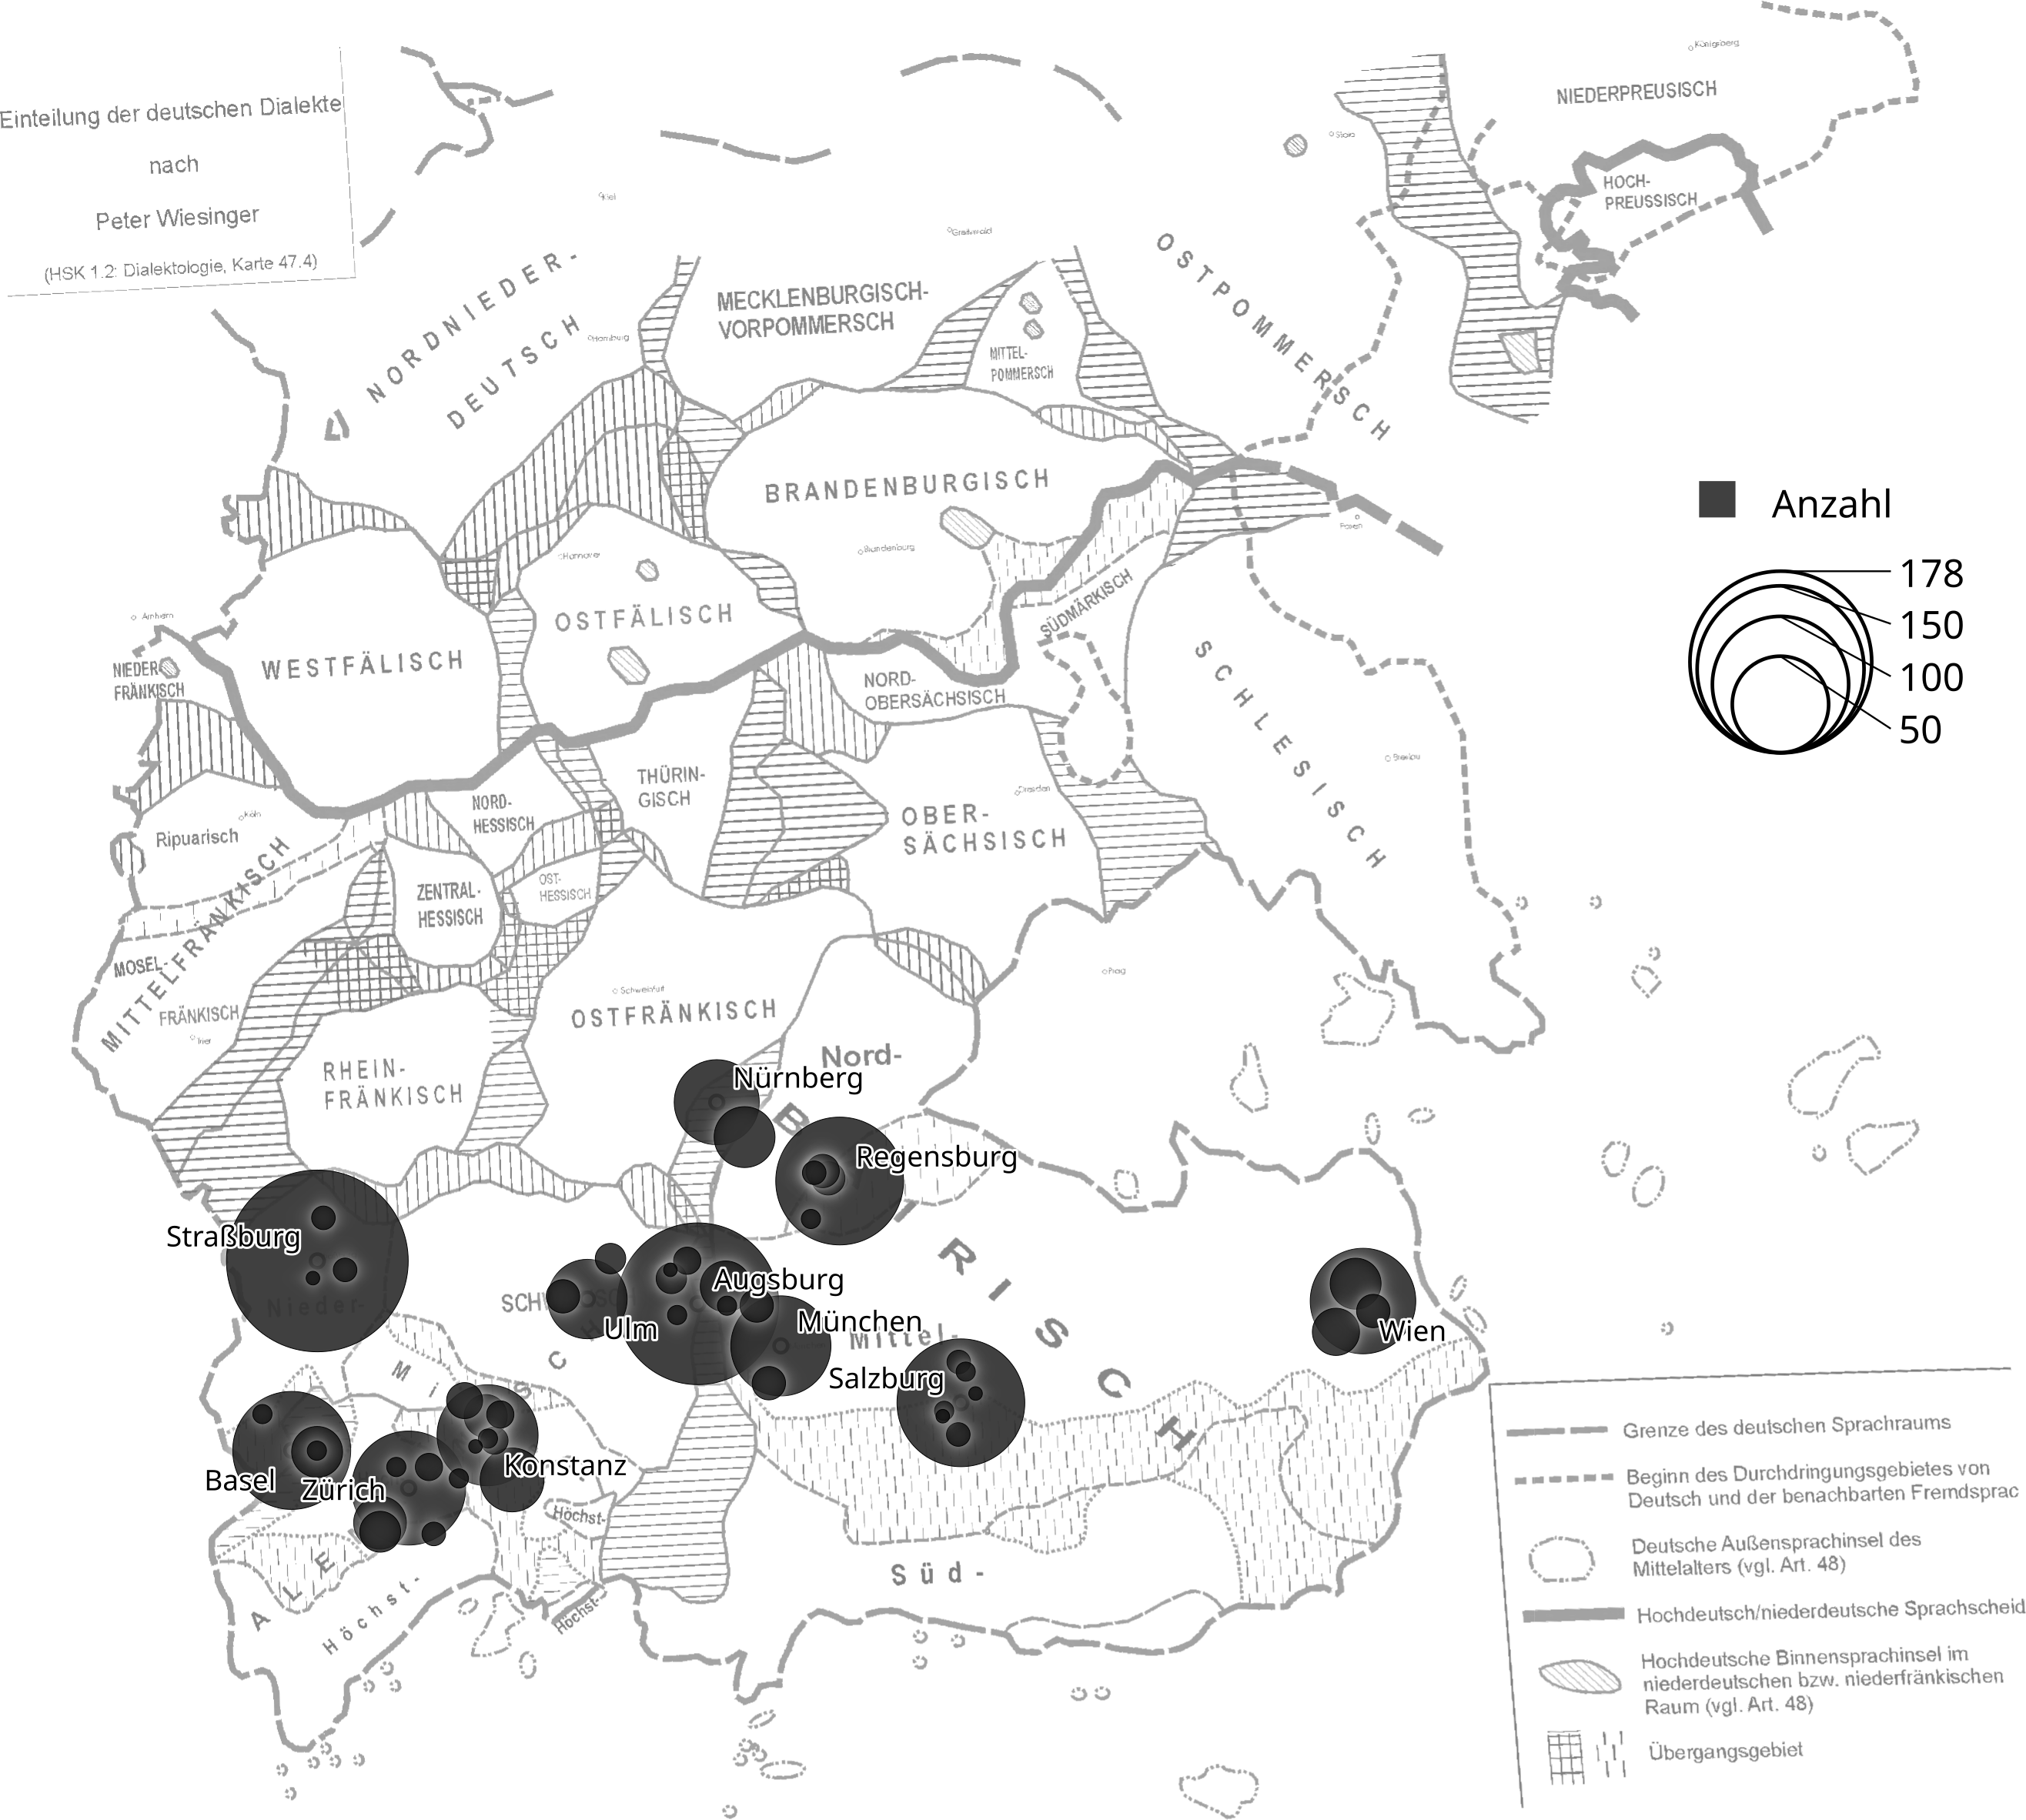
\includegraphics[
	width=\linewidth,
	keepaspectratio
]{./figures/2021-05-10_adjektivstichprobe_cao.png}
\caption{Menge der Belege pro Ausstellungs\-ort in der Stichprobe zur
	Adjektivdeklination (Hintergrundkarte: \cite{wiesinger1983:rede})}
\label{fig:adjstpr_orte}
\end{figure}

Zusätzlich wurden für alle in \tabref{tab:adjstpr_orte} aufgelisteten
Ausstellungs\-orte noch alle weiteren Orte im Umkreis von etwa vierzig
Kilometern (0,25°) hinzugenommen, gerade auch, was Nürnberg, München und Ulm
betrifft, für die jeweils nur wenige Urkunden zur Verfügung stehen. Mögliche
schreibsprachliche Unterschiede zwischen Stadt und Umland sowie die Lage
Augsburgs im Übergangsgebiet vom Schwäbischen\il{Schwäbisch} zum
Bairischen\il{Bairisch} wurden dabei außer Acht gelassen, zumal hier nicht
phonologische, sondern morphosyntaktische Variation angesprochen wird. Bei der
Durchsicht und Klassifizierung der Belege erwies sich dieser Vorbehalt als
unproblematisch.

Für die Anfertigung der Stichprobe ist es nur bedingt nützlich, automatisiert
alle jeweiligen Formen für einen bestimmten Ort ausgeben zu lassen, da die
automatische Wortartzuordnung des Taggers bei Adjektiven nicht zuverlässig
funktioniert und die Wortformenbestimmung teils Lücken aufweist oder ebenso
ungenau ist. Daher wurde zur Auswahl häufiger Lemmata eine Liste aller im
\WMU{} verzeichneten Lemmata mit der dort angegebenen Häufigkeit\is{Frequenz}
herangezogen.%
%
	\footnote{Die Liste (mit Stand 2009) wurde der AG~Sprachgeschichte der
	Philipps-Universität Marburg 2013 im Rahmen erster Studien zum
	\CAO{} von \iai{Ursula Schulze} (†) zur Verfügung gestellt.}
	%
	% U.S. an Jürg Fleischer am 13.02.2013 15:11 Uhr
	% J.F. an Oliver Schallert am 14.02.2013 08:54 Uhr
	% O.S. an mich (Beckerc2@students) am 16.02.13 18:59 Uhr
%
Die Auswahl fiel dabei auf die in \tabref{tab:adjsmpwords} aufgelisteten
Lemmata. Um Irrläufer\is{Falschpositiv} zu vermeiden, wurden nur diejenigen
Belege für die einzelnen Lemmata aus der \isi{Datenbank} extrahiert, die der
Tagger von \citet{schmid2019} mit mindestens 95-prozentiger Sicherheit dem
jeweiligen Lemma zuordnen konnte.

\begin{table}[h]
\centering
\caption{Lemmata der Stichprobe}
\begin{tabular}{l l r l @{\citereset}}
\lsptoprule

Lemma
	& Übersetzung
	& Häufigkeit\is{Frequenz}
	& Quelle
	\\

\midrule
\norm{ēhaft}
	& `rechtsgültig'
	& 105
	& \cite[419--420]{wmu1}
	\\
\norm{ēlich}
	& `rechtmäßig'
	& 350
	& \cite[448--449]{wmu1}
	\\
\norm{ganƶ}
	& `ganz'
	& 631
	& \cite[549--550]{wmu1}
	\\
\norm{grōȥ}
	& `groß'
	& 270
	& \cite[761--762]{wmu1}
	\\
\norm{guet}
	& `gut'
	& 1.643
	& \cite[770--772]{wmu1}
	\\
\norm{klėine}
	& `klein'
	& 116
	& \cite[1011--1012]{wmu2}
	\\

\norm{niuwe}
	& `neu'
	& 355
	& \cite[1322--1324]{wmu2}
	\\

\lspbottomrule

\end{tabular}
\label{tab:adjsmpwords}
\end{table}

Die häufigsten Adjektive, die oft in festen Fügungen wie den eingangs zitierten
auftreten, wurden bei der Auswahl der Lemmata vermieden. Possessivbegleiter --
hauptsächlich \norm{mīn} `mein' (11.250 Belege; \cite[1231--1232]{wmu2}) --
wurden aufgrund ihrer Häufigkeit\is{Frequenz} verwendet, um Lücken aufzufüllen,
abgesehen vom Nom.\ Sg. aller Genera\is{Genus} sowie dem Akk.\ Sg.\ N., wo
häufig auch eine Form ohne Flexion steht \autocites[216]{paul2007}[507,
510--511]{ksw2}. Allerdings ist anzumerken, dass \norm{mīn} `mein' bisweilen
auch im Nom./Akk.\ Pl.\ M./F. unflektiert auftritt. \citet[510]{ksw2} fassen
dies \blockquote{im Wesentlichen \textins{als} Resultat der vom Oobd.
ausgehenden Schwa-\isi{Apokope}} auf. Sie weisen aber auch darauf hin, dass
daneben flektiertes \norm{alle} (mit Schwa) vor unflektiertem
\norm{mīn}/\norm{dīn}/\norm{sīn} `mein'/`dein'/`sein' keine Seltenheit in ihrem
Korpusmaterial darstellt. Entsprechende Belege wurden deshalb hier
ausgeklammert.

Für das Alemannische\il{Alemannisch} weisen \citet[271, Abbildung~A~47]{ksw2}
für die zweite Hälfte des 13.~Jahrhunderts 10\,\% flexionslose Formen bei
vorangestellten Adjektiven in Positionen mit regulärem \norm{e}-Flexiv aus,
34\,\% für die erste Hälfte des 14.~Jahrhunderts; Schwäbisch\il{Schwäbisch}
wird nicht gesondert verzeichnet. Bei den Pluralbelegen in der Stichprobe aus
Urkunden des \CAO{} fällt auf, dass unflektiertes \norm{mīn} `mein' in allen
Fällen vor \norm{ėrben} `Erben' steht, wobei das Fehlen der Flexion hier auch
auf Hiatusvermeidung zurückgeführt werden kann.

Noch bestehende Lücken wurden durch manuelle Durchsicht der Urkundentexte zum
jeweiligen Ort gefüllt, wobei darauf geachtet wurde, nach Möglichkeit wenigstens
zwei Belegstellen zu finden und dabei Variation zu berücksichtigen. Die
Annotation\is{Annotation} der Belege geschah in jedem Fall manuell. Belege, bei
denen das Lemma bei der automatischen Annotation\is{Annotation} falsch
zugeordnet wurde, wurden übergangen. Die Tabellen im
Anhang~\ref{sec:caoadjquanttab} listen die ausgewerteten Belegmengen pro
Bezugsort mit den hinzugezogenen Ausstellungs\-orten in dessen Umkreis auf. Im
Folgenden sollen kurz die Belege zum Nom./Akk.\ Sg.\ F.\ und Pl.\ pro
untersuchtem Ort charakterisiert werden.

\subsection{Diskussion}
\label{subsec:cao_adjflex_disc}

\il{Alemannisch|(}
\subsubsection{Straßburg}
\label{par:adjstrassburg}
In Straßburger Urkunden wird regelmäßig kein Unterschied zwischen \norm{e}- und
\norm{iu}-Formen gemacht \REF{ex:adjstrbgregel}. In der Stichprobe sind
außerdem zwei Belege zu \norm{ērbǟre} `ehrenhaft, edel' mit \lit{-i} für den
Nom.\ Sg.\ F.\ enthalten \REF{ex:adjstrbgi_1}. Auch für den Nom./Akk.\ Pl.\ N.\
ist einmal \lit{-i} in der Stichprobe enthalten \REF{ex:adjstrbgi_3}, sowie
viermal \lit{-u/-û} neben regelmäßigem \lit{-e} \REF{ex:adjstrbgu}, davon ein
Doppelbeleg für \norm{kristenlich} `christlich' mit \lit{-u} und
\lit{-e} \REF{ex:adjstrbgu_1}. Die betreffenden Belege stammen alle aus
Straßburg selbst.

\begin{exe}
\ex \label{ex:adjstrbgregel}
	\begin{xlist}
	\ex \label{ex:adjstrbgregel_1}
		\gll ir erſame botten \\
			ihr ehrbar-\textsc{nom.pl.\MascM.st} Bevollmächtigten \\
		\trans `ihre ehrsamen Bevollmächtigten'
			\parencites(Nr.~N~7, Straßburg, 1262)[7,39]{cao5}

	\ex \label{ex:adjstrbgregel_2}
		\gll ander cleine vorderunge \\
			ander klein-\textsc{nom.pl.\FemI.st} Forderungen \\
		\trans `andere kleine Forderungen'
			\parencites(Nr.~N~14, Straßburg, 1262?)[14,3]{cao5}

	\ex \label{ex:adjstrbgregel_3}
		\gll ſint vnsere ingeſigele an diſen brief gehenket \\
			sind unser-\textsc{nom.pl.\NeutI.st} Siegel an diesen Brief gehängt \\
		\trans `sind unsere Siegel an diese Urkunde gehängt'
			\parencites(Nr.~N~227, Straßburg, 1283)[174,4]{cao5}
	\end{xlist}

\ex \label{ex:adjstrbgi}
	\begin{xlist}
	\ex{\label{ex:adjstrbgi_1}
		\let\eachwordthree\eachwordtwo
		\let\eachwordtwo\eachwordone
		\glll dîe êrberi frowe \\
			dú erberi frowe \\
			\textsc{def.nom.sg.\FemF} ehrhaft-\textsc{nom.sg.\FemF.st} Edelfrau \\
		\trans `die ehrhafte Edelfrau'
			\parencites(Nrn.~N~109~AB, Straßburg, 1272)[79,21]{cao5}}

	\ex \label{ex:adjstrbgi_3}
		\gll Vnſeri kint \\
			unser-\textsc{nom.pl.\NeutX.st} Kind \\
		\trans `unsere Kinder'
			\parencites(Nr.~N~142, Straßburg, 1276)[100,18]{cao5}
	\end{xlist}
\end{exe}

\begin{exe}
\ex \label{ex:adjstrbgu}
	\begin{xlist}
	\ex{\label{ex:adjstrbgu_1}
		\let\eachwordthree\eachwordtwo
		\let\eachwordtwo\eachwordone
		\glll A: alle criſtenliche dinc \\
			B: allv criſtenlichu dinc \\
			{} alle-\textsc{acc.pl.\NeutI} christlich-\textsc{acc.pl.\NeutI.st} Ding \\
		\trans `alle christlichen Dinge'
			\parencites(Nrn.~N~10~AB, Straßburg, 1262)[9,20--21]{cao5}}

	\ex \label{ex:adjstrbgu_3}
		\gll vnſerû kint \\
			unser-\textsc{acc.pl.\NeutX} Kind \\
		\trans `unsere Kinder'
			\parencites(Nr.~2663, Straßburg, 1297)[62,35]{cao4}

	\ex \label{ex:adjstrbgu_4}
		\gll vnſerû jngeſigele \\
			unser-\textsc{acc.pl.\NeutI} Siegel \\
		\trans `unsere Siegel'
			\parencites(Nr.~2663, Straßburg, 1297)[63,25]{cao4}
	\end{xlist}
\end{exe}

Da \lit{-i} und \lit{-u} in der Regel an Stellen erscheinen, an denen nach dem
oberdeutschen\il{Oberdeutsch} Flexionsparadigma mit \norm{-iu} zu
rechnen ist, kann davon ausgegangen werden, dass diese beiden Grafien nicht
\norm{-e} zuzuordnen sind, obwohl \lit{-i} für \norm{-e} noch in der zweiten
Hälfte des 13.~Jahrhunderts im Alemannischen\il{Alemannisch} belegt ist
\autocites[41]{paul2007}[305]{ksw2}[vgl.~auch][466--467]{schirmunski1962}. Bei
der Teiluntersuchuchung im Anhang~\ref{sec:caoalemschwa} zur Grafie von
mittelhochdeutsch unbetontem \norm{e} [ə] traten bei den gewählten
nicht-adjektivischen Lexemen in Straßburg keine \lit{i}-Schreibungen auf.

\subsubsection{Basel}
\label{par:adjbasel}
Für Basel haben sich auch bei manueller Durchsicht keine Belege für Formen des
Nom./Akk.\ Sg./Pl.\ F.\ finden lassen. Dennoch zeigt sich hier zumindest für
Maskulina und Neutra klarer als in Straßburg die für das
Oberdeutsche\il{Oberdeutsch} typische Unterscheidung zwischen \norm{e}- und
\norm{iu}-Typen, die in der Regel durch \lit{-e} und \lit{-u/-ú} vertreten sind
\REF{ex:adjbaselregel}. Für den Akk.\ Pl.\ N.\ ist jeweils ein Beleg für
\norm{-iu} und einer für \norm{-e} in der Stichprobe enthalten
\REF{ex:adjbaselu}.

\begin{exe}
\ex \label{ex:adjbaselregel}
	\begin{xlist}
	\ex \label{ex:adjbaselregel_1}
		\gll anden vorgenanten hern peter vn̄ ſine erben \\
			an=den vorgenannten Herrn Peter und sein-\textsc{acc.pl.\MascM.st}
				Erben \\
		\trans `an den vorgenannten Herrn Peter und seine Erben'
			\parencites(Nr.~1682, Basel, 1293)[16,15--16]{cao3}

	\ex \label{ex:adjbaselregel_2}
		\gll minu kint dú vorgenanten \\
			mein-\textsc{nom.pl.\NeutMF} Kind die vorgenannten \\
		\trans `meine Kinder, die vorgenannten'
			\parencites(Nr.~3184, Rheinfelden, Kt.~Aargau, 1299)[376,13]{cao4}
	\end{xlist}

\ex \label{ex:adjbaselu}
	\begin{xlist}
	\ex \label{ex:adjbaselu_1}
		\gll fur Minv kint Walthern vn̄ hennrichen vn̄ Rvͦdolfen \\
			für mein-\textsc{acc.pl.\NeutM.st} Kind Walther-\textsc{obl} und
			Heinrich-\textsc{obl} und Rudolf-\textsc{obl} \\
		\trans `für meine Kinder Walther und Heinrich und Rudolf'
			\parencites(Nr.~1108, Basel, 1289)[402,36--37]{cao2}

	\ex \label{ex:adjbaselu_2}
		\gll in mine vaſ \\
			in mein-\textsc{acc.pl.\NeutI.st} Fass \\
		\trans `in meine Fässer'
			\parencites(Nr.~N~483, Mulhouse, Dépt.~Haut-Rhin, 1291)[351,23]{cao5}
	\end{xlist}
\end{exe}

\subsubsection{Zürich}
\label{par:adjzuerich}
Auch in Zürich zeigt sich zumindest im Plural die typische
oberdeutsche\il{Oberdeutsch} Verteilung\is{Distribution!morphologische} von
\norm{e}- und \norm{iu}-Typen, die hier in der Regel durch \lit{-e} und \lit{-ú}
repräsentiert sind \REF{ex:adjzuerregel}. Für den Nom.\ Sg.\ F.\ ist in der
Stichprobe sowohl ein Beleg für \norm{-iu} als auch für \norm{-e} enthalten
\REF{ex:adjzueru}. Diese stammen allerdings nicht aus Zürich selbst, sondern aus
dem ca.\ 40~km in südöstlicher Richtung liegenden Hohenrain (Kt.~Luzern).

\begin{exe}
\ex \label{ex:adjzuerregel}
	\begin{xlist}
	\ex \label{ex:adjzuerregel_1}
		\gll zewene geliche brieue \\
			zwei[\MascI] gleich-\textsc{acc.pl.\MascI.st}
				Urkunde-\textsc{acc.pl.\MascI} \\
		\trans `zwei gleiche Urkunden'
			\parencites(Nr.~2209, Zürich, 1295)[364,33]{cao3}

	\ex \label{ex:adjzuerregel_2}
		\gll ich herre walther vn̄ minu kint \\
			ich Herr Walther und mein-\textsc{nom.pl.\NeutX.st} Kind \\
		\trans `ich, Herr Walther, und meine Kinder'
			\parencites(Nr.~456, Hohenrain, Kt.~Luzern, 1281)[396,33--34]{cao1}
	\end{xlist}

\ex \label{ex:adjzueru}
	\begin{xlist}
	\ex \label{ex:adjzueru_1}
		\gll min elichú huſvrowͮe \\
			mein rechtmäßig-\textsc{nom.sg.\FemF.st} Ehefrau \\
		\trans `meine rechtmäßige Ehefrau'
			\parencites(Nr.~260, Hohenrain, Kt.~Luzern, 1276)[271,9]{cao1}

	\ex \label{ex:adjzueru_2}
		\gll mín êliche wirten \\
			mein rechtmäßig-\textsc{nom.sg.\FemF.st} Ehefrau \\
		\trans `meine rechtmäßige Ehefrau'
			\parencites(Nr.~1888, Hohenrain, Kt.~Luzern, 1294)[173,11]{cao3}
	\end{xlist}
\end{exe}

Neben zwei Belegen mit \lit{rechte} `rechtmäßige' im Akk.\ Sg.\ F.\
entsprechend dem in \REF{ex:adjzuere_1} finden sich auch zwei mit \lit{rechtú}
für denselben syntaktischen Kontext wie in \REF{ex:adjzuere_3};
\citet[vgl. dazu][270--271]{ksw2}. Bei den letzeren zwei Urkunden handelt es
sich um eine Urkunde und ihre Bestätigung \autocite[375]{caor}. Für beide ist
Zürich als Ausstellungs\-ort angegeben.

\begin{exe}
\ex \label{ex:adjzuere}
	\begin{xlist}
	\ex \label{ex:adjzuere_1}
		\gll in rechte giſelſchaft \\
			in recht-\textsc{acc.sg.\FemI.st} Geiselschaft \\
		\trans `in rechtsgemäße Geiselschaft'
			\parencites(Nr.~35, Zürich, 1256 und Nr.~188, ebd., 1272)[66,31; 204,31]{cao1}

	\ex \label{ex:adjzuere_3}
		\gll das es rechtú not tête \\
			dass es recht-\textsc{acc.sg.\FemI.st} Not täte \\
		\trans `dass es von Rechts wegen erforderlich wäre'
			\parencites(Nr.~1591, Zürich, 1292 und Nr.~1756, ebd., 1292/93)[731,3]{cao2}[67,26--27]{cao3}
	\end{xlist}
\end{exe}

Daneben ist die Häufung von Belegen ohne overte Markierung\is{Genusmarkierung}
im Nom./Akk.\ Pl.\ M.\ auffällig: 3 Belegen mit \norm{-e} stehen 9 ohne
Flexionsendung gegenüber. Bei diesen unflektierten Belegen handelt es sich
sämtlich um Vorkommen des Possessivpronomens \norm{mīn} `mein' wie in
(\ref{ex:adjzuer0_1}--b), die flektiertem \norm{mine} `meine'
\REF{ex:adjzuer0_3} und \norm{geliche} `gleiche' gegenüberstehen. Ein Beleg
für \norm{mīn} und der für \norm{mīne} stammen nicht aus Zürich selbst, sondern
aus Eschenbach (Kt.~Luzern), etwa 45~km südwestlich von Zürich und 10~km
nordöstlich von Luzern. Selbst wenn diese zwei Belege nicht gezählt werden,
ändert sich das Bild nicht grundlegend.

\begin{exe}
\ex \label{ex:adjzuer0}
	\begin{xlist}
	\ex \label{ex:adjzuer0_1}
		\gll ſo ſvln min erbin · diz {vol fvͦrin.} \\
			so sollen mein[\textsc{nom.pl.\MascA}] Erben {} dies ausführen \\
		\trans `so sollen meine Erben dies ausführen'
			\parencites(Nr.~19, Zürich, 1251)[28,20]{cao1}

	\ex \label{ex:adjzuer0_2}
		\gll fúr mich / vnd min nachkomen \\
			für mich {} und mein[\textsc{acc.pl.\MascA}] Nachkommen \\
		\trans `für mich und meine Nachkommen'
			\parencites(Nr.~2051~A, Zürich, 1294)[278,25--26]{cao3}

	\ex \label{ex:adjzuer0_3}
		\gll fv̓r alle mine nahkomen alde mine erben \\
			für alle mein-\textsc{acc.pl.\MascA.st} Nachkommen oder
				mein-\textsc{acc.pl.\MascA.st} Erben \\
		\trans `für alle meine Nachkommen oder meine Erben'
			\parencites(Nr.~1982, Eschenbach, Kt.~Luzern, 1294)[239,20--21]{cao3}
	\end{xlist}
\end{exe}

Generell erscheinen im Raum Zürich Formen des Nom./Akk.\ Pl.\ M.\ anders
markiert als solche des Nom./Akk.\ Pl.\ N.

\subsubsection{Konstanz}
\label{par:adjkonst}
Die Belegverteilung\is{Distribution!morphologische} in Urkunden aus der
Bodenseeregion um Konstanz weist die für das oberdeutsche\il{Oberdeutsch}
typische Differenzierung zwischen \norm{e}- und \norm{iu}-Typen auf
\REF{ex:adjkonstregel}, letztere treten auch grafisch als \lit{iu} in
Erscheinung (in St.~Galler Urkunden auch als \lit{vͥ}). Daneben sind wenige
flexionslose Belege in Positionen des Paradigmas enthalten, in denen ansonsten
regelmäßig \norm{e} steht, nämlich einmal im Akk.\ Sg.\ F.\ \REF{ex:adjkonstesg}
sowie viermal im Nom.\ Pl.\ M.\ \REF{ex:adjkonstepl}.

\begin{exe}
\ex \label{ex:adjkonstregel}
	\begin{xlist}
	\ex \label{ex:adjkonstregel_1}
		\gll Huc · Cvͦnrade · vͦlrich · vn̄ Johanſ mine ſv̓ne \\
			Hugo {} Konrad {} Ulrich {} und Johannes
				mein-\textsc{nom.pl.\MascM.st} Söhne \\
		\trans `Hugo, Konrad, Ulrich und Johannes, meine Söhne'
			\parencites(Nr.~2654, Konstanz, 1297)[57,33]{cao4}

	\ex \label{ex:adjkonstregel_2}
		\gll wir die aigeniv Jngeſigel hant \\
			wir die eigen-\textsc{acc.pl.\NeutI.st} Siegel haben \\
		\trans `wir, die eigene Siegel haben'
			\parencites(Nrn.~530~AB, Konstanz, 1282)[468,3--4]{cao1}
	\end{xlist}

\ex \label{ex:adjkonstesg}
	\begin{xlist}
	\ex \label{ex:adjkonstesg_1}
		\gll mine tohter \\
			mein-\textsc{acc.sg.\FemF.st} Tochter \\
		\trans `meine Tochter'
			\parencites(Nr.~2226, Überlingen, Bodenseekr., 1295)[373,42]{cao3}

	\ex \label{ex:adjkonstesg_2}
		\gll fur min muͦter \\
			für mein[\textsc{acc.sg.\FemF}] Mutter \\
		\trans `für meine Mutter'
			\parencites(Nr.~530~B, Konstanz, 1282)[464,12]{cao1}
	\end{xlist}
\end{exe}

\begin{exe}
\ex \label{ex:adjkonstepl}
	\begin{xlist}
	\ex \label{ex:adjkonstepl_1}
		\gll mine ſv̓ne \\
			mein-\textsc{nom.pl.\MascM.st} Söhne \\
		\trans `meine Söhne'
			\parencites(Nr.~2654, Konstanz, 1297)[57,44]{cao4}

	\ex \label{ex:adjkonstepl_2}
		\gll {des ſelben} huſes reht erben \\
			desselben Hauses recht[\textsc{nom.pl.\MascA}] Erben \\
		\trans `desselben Hauses rechtmäßige Erben'
			\parencites(Nr.~2675, Konstanz, 1297)[71,34]{cao4}
	\end{xlist}
\end{exe}
\il{Alemannisch|)}

\il{Schwäbisch|(}
\subsubsection{Ulm}
\label{par:adjulm}
Die Stichprobe zu Ulm verhält sich vollkommen unauffällig: Es wird klar
zwischen \norm{-e} und \norm{-iu} geschieden, beide Typen sind auch in der
Grafie regelmäßig so realisiert \REF{ex:adjulm}.

\begin{exe}
\ex \label{ex:adjulm}
	\begin{xlist}
	\ex \label{ex:adjulm_1}
		\gll ander biderbe lute \\
			ander brav-\textsc{nom.pl.\MascX.st} Leute \\
		\trans `andere brave Leute'
			\parencites(Nr.~3308, Ulm, 1299)[455,44]{cao4}

	\ex \label{ex:adjulm_2}
		\gll mine vorginanten froͤwen von Sovelingen \\
			mein-\textsc{nom.pl.\FemF.st} vorgenannten Frauen von Söflingen \\
		\trans `meine vorgenannten Frauen von Söflingen'
			\parencites(Nr.~2467, Ulm, 1296)[526,36]{cao3}

	\ex \label{ex:adjulm_3}
		\gll vnſeriv Jnſigel \\
			unser-\textsc{acc.pl.\NeutI.st} Siegel \\
		\trans `unsere Siegel'
			\parencites(Nr.~1662, Ulm, 1293)[3,12--13]{cao3}
	\end{xlist}
\end{exe}

\subsubsection{Augsburg}
\label{par:adjaugsburg}
Auch in Augsburg wird bei der starken Adjektivdeklination klar zwischen
\norm{e}- und \norm{iu}-Typen unterschieden \REF{ex:adjaugs}. Für den letzeren
ist für Augsburg selbst hauptsächlich \lit{iuͤ} neben einfachem \lit{iu}
bezeugt; im ca. 23~km in nordöstlicher Richtung entfernten Aichach findet sich
regelmäßig \lit{u} in \lit{minu} `meine'. Auffällige Unterschiede im
Gebrauch zwischen Stadt und Umland machen sich auch hier nicht bemerkbar.

\begin{exe}
\ex \label{ex:adjaugs}
	\begin{xlist}
	\ex \label{ex:adjaugs_1}
		\gll zwen erbere man \\
			zwei[\MascM] ehrenhaft-\textsc{nom.pl.\MascM.st} Mann \\
		\trans `zwei ehrenhafte Männer'
			\parencites(Nr.~1270, Augsburg, 1290)[508,40]{cao2}

	\ex \label{ex:adjaugs_2}
		\gll gvͤte Hantveſte \\
			gut-\textsc{acc.pl.\FemI.st} Urkunde \\
		\trans `gültige Urkunden'
			\parencites(Nr.~3471, Augsburg, 1299)[557,21]{cao4}

	\ex \label{ex:adjaugs_3}
		\gll Ane minivͤ Manlehen \\
			ohne mein-\textsc{acc.pl.\NeutI.st} Mannslehen \\
		\trans `ohne meine Mannslehen'
			\parencites(Nr.~1363, Augsburg, 1291)[586,9]{cao2}
	\end{xlist}
\end{exe}
\il{Schwäbisch|)}

\il{Ostfränkisch|(}
\subsubsection{Nürnberg}
\label{par:adjnuernberg}
Die Belege der Stichprobe zu Nürnberg zeigen ebenfalls keine Auffälligkeiten in
der Verteilung\is{Distribution!morphologische}. Allein die relativ geringe
Belegmenge führt dazu, dass für den Akk.\ Pl.\ M. sowie für den Nom./Akk.\ Pl.\
F.\ keine Belege gefunden werden konnten. Da \norm{-e} im Akk.\ Sg.\ F.\ und im
Nom.\ Pl.\ M. ansonsten aber erwartungsgemäß \norm{-iu} (geschrieben ebenfalls
\lit{iu}) im Nom.\ Sg.\ F.\ und Nom./Akk.\ Pl.\ N.\ gegenübersteht, kann mit
etwas Vorsicht davon ausgegangen werden, dass der Regelfall auch hier gilt.

\begin{exe}
\ex \label{ex:adjnuern}
	\begin{xlist}
	\ex \label{ex:adjnuern_1}
		\gll ich vn̄ mine ſvne \\
			ich und mein-\textsc{nom.pl.\MascM.st} Söhne \\
		\trans `ich und meine Söhne'
			\parencites(Nr.~3428, Kl.~Seligenporten, Kr.~Neumarkt in der Oberpfalz, 1299)[525,15]{cao4}

	\ex \label{ex:adjnuern_2}
		\gll daz vnſ ehaftiv not irre \\
			dass uns rechtsgültig-\textsc{nom.sg.\FemI.st} Not hindere \\
		\trans `dass wir aus einem rechtsgültigen Grund verhindert sind'
			\parencites(Nr.~949, Nürnberg, 1287)[301,12--13]{cao2}

	\ex \label{ex:adjnuern_3}
		\gll do vnſeriv chint \\
			als unser-\textsc{nom.pl.\NeutX.st} Kind \\
		\trans `als unsere Kinder'
			\parencites(Nrn.~1972~AB, Nürnberg, 1294)[225,17--18]{cao3}
	\end{xlist}
\end{exe}

\subsubsection{Regensburg}
\label{par:adjregensburg}
Die exzerpierten Stellen aus Regensburger Urkunden verhalten sich regelmäßig.
Auch hier besteht die Schwierigkeit, dass sich keine Belege für den Nom./Akk.\
Pl.\ F.\ haben finden lassen. Im Singular sowie zwischen Plural Maskulinum und
Neutrum zeigt sich jedoch klar der Formenunterschied; \norm{iu}~/yː/ ist
diphthonigiert als \lit{eu} repräsentiert. Die Schwa-\isi{Apokope}
\autocites{lindgren1953}[109--111]{paul2007} macht sich hier bemerkbar,
insofern an Stellen des Paradigmas, die sonst regelmäßig \norm{-e} aufweisen,
die Endung fehlen kann \REF{ex:adjregbge}.%

\begin{exe}
\ex \label{ex:adjregbge}
	\begin{xlist}
	\ex \label{ex:adjregbge_3}
		\gll an vbel liſte \\
			ohne schlecht[\textsc{acc.pl.\MascI}] Absichten \\
		\trans `ohne schlechte Absichten'
			\parencites(Nr.~1970, Laaber, Kr.~Regensburg, 1294)[224,26]{cao3}

	\ex \label{ex:adjregbge_1}
		\gll ander erſame levte \\
			ander ehrsam-\textsc{nom.pl.\MascA.st} Leute \\
		\trans `andere ehrsame Leute'
			\parencites(Nr.~3404, Regensburg, 1299)[507,43]{cao4}

	\ex \label{ex:adjregbge_2}
		\gll an ein new ſetze \\
			ohne ein neu[\textsc{acc.sg.\FemI}] Rebpflanzung \\
		\trans `ausgenommen eine neue Rebpflanzung'%
			\footnote{Siehe \citet[\nopp 102]{caor}; \citet[s.\,v.~\fw{setze}]{%
				lexer:mhdhwb} definiert \norm{sėƶƶe} in diesem Zusammenhang als
				\textquote{ein mit reben besetztes grundstück von bestimmter
				grösse} und bestimmt es als starkes Femininum.}
			%
			\parencites(Nr.~N~447, Regensburg, 1290)[328,38]{cao5}
	\end{xlist}
\end{exe}
\il{Ostfränkisch|)}

\il{Bairisch|(}
\subsubsection{München}
\label{par:adjmuenchen}
Mehr noch als in Regensburg macht sich in der Stichprobe zu München die
Schwa-\isi{Apokope} bemerkbar, insofern an allen Stellen, die sonst regelgemäß
\norm{-e} haben, die Endung häufig fehlt. Der Flexionstyp \norm{-iu} weist
auch hier die Form \lit{-iu} auf, neben der bairischen Form \lit{-eu}. Beide
Flexionstypen verteilen sich regelmäßig: -Ø steht systematisch also einer
Grafie vom Typ \norm{-iu} gegenüber \REF{ex:adjmuench}.

\begin{exe}
\ex \label{ex:adjmuench}
	\begin{xlist}
	\ex \label{ex:adjmuench_1}
		\gll zwo erbwær iunchfrawen \\
			zwei[\FemF] ehrenhaft[\textsc{acc.pl.\FemF}] Jungfrauen \\
		\trans `zwei ehrenhafte junge Frauen'
			\parencites(Nr.~1024, München, 1288)[348,21]{cao2}

	\ex \label{ex:adjmuench_2}
		\gll ſiniv kint \\
			sein-\textsc{nom.pl.\NeutA.st} Kind \\
		\trans `seine Kinder'
			\parencites(Nr.~2371, München, 1296)[473,9]{cao3}
	\end{xlist}
\end{exe}

\subsubsection{Salzburg}
\label{par:adjsalzburg}
Die Belege zu Salzburger Urkunden verhalten sich ähnlich zu den Belegen zu
München. Auch hier wird regelmäßig zwischen den Typen \norm{-e} und
\norm{-iu} unterschieden, die als \lit{-e}/-Ø beziehungsweise \lit{-eu}
grafischen Ausdruck finden \REF{ex:adjsalzbg}.

\begin{exe}
\ex \label{ex:adjsalzbg}
	\begin{xlist}
	\ex \label{ex:adjsalzbg_1}
		\gll ærwer / vnt ehaft ſache \\
			ehrenhaft[\textsc{nom.sg.\FemI}] {} und rechtsgültig[\textsc{nom.sg.\FemI}]
				Sache \\
		\trans `ehrenhafter und rechtsgültiger Grund'
			\parencites(Nr.~818, Bad Reichenhall, Kr.~Berchtesgadener Land, 1286)[177,1--2]{cao2}

	\ex \label{ex:adjsalzbg_2}
		\gll vmb ander niwe veſt \\
			um ander neu-\textsc{acc.pl.\FemI.st} Burg \\
		\trans `bezüglich anderer neuer Burgen'
			\parencites(Nr.~695, Salzburg, um 1285)[104,19]{cao2}

	\ex \label{ex:adjsalzbg_3}
		\gll dev vorgenantev gvͦt \\
			die vorgenannt-\textsc{acc.pl.\FemI.st} Gut \\
		\trans `die vorgenannten Güter'
			\parencites(Nr.~2446, Salzburg, 1296)[514,11--12]{cao3}
	\end{xlist}
\end{exe}

Darüber hinaus tritt einmal \lit{Newev} `neue' mit einer \norm{iu}-Form
statt der gewöhnlichen \norm{e}-Form im Akk.\ Sg.\ F.\ auf
\REF{ex:adjsalzbgirr_1}. Mit \citet{ksw2} lässt sich vermuten, dass es sich
dabei um \blockcquote[270]{ksw2}{\mbox{eine} Angleichung an den
Nom.~Sg.~fem.~stark} handelt, die sie als möglicherweise schwerpunktmäßig
bairisch betrachten.

\begin{exe}
	\ex \label{ex:adjsalzbgirr_1}
		\gll der ein Newev veſte gebown hat \\
			der ein neu-\textsc{acc.sg.\FemI.st} Burg gebaut hat \\
		\trans `der eine neue Burg gebaut hat'
			\parencites(Nr.~695, Salzburg, um 1285)[103,11]{cao2}
\end{exe}

\subsubsection{Wien}
\label{par:adjwien}
Auch für Wien lässt sich ein klarer Unterschied zwischen \norm{e}- und
\norm{iu}-Typen in der Flexion ausmachen, die sich regelmäßig in den Grafien
\lit{-e/-Ø} und \lit{-eu/-iu} manifestiert. Für den Plural hat es sich
allerdings als schwierig herausgestellt, eindeutige Belege für starke Maskulina
und Feminina zu finden. Diese stehen jeweils mit \isi{Apokope}
\REF{ex:adjwienapo}. Für den Akk.\ Sg.\ F.\ fanden sich die Formen in
\REF{ex:adjwienakksgf}.

\begin{exe}
\ex \label{ex:adjwienapo}
	\begin{xlist}
	\ex \label{ex:adjwienregel_1}
		\gll wider mein gêrben \\
			gegen mein[\textsc{nom.pl.\MascM}] Erben \\
		\trans `gegen meinen Erben'
			\parencites(Nr.~N~263, Wien, 1284)[210,24]{cao5}

	\ex \label{ex:adjwienregel_2}
		\gll brief vnd grozz hantveſt \\
			Urkunde und groß[\textsc{acc.pl.\FemI}] Urkunde \\
		\trans `Briefe und große Urkunden'
			\parencites(Nr.~67, Stift~Heiligenkreuz, Bz.~Baden, 1263)[103,21]{cao1}
	\end{xlist}

\ex \label{ex:adjwienakksgf}
	\begin{xlist}
	\ex \label{ex:adjwienakksgf_1}
		\gll dvrch rehte notdvrft \\
			durch recht-\textsc{acc.sg.\FemI.st} Notlage \\
		\trans `aufgrund der rechtsgültigen Notlage'
			\parencites(Nr.~2966, Wien, 1298)[243,3]{cao4}

	\ex \label{ex:adjwienakksgf_2}
		\gll ain halbe wiſe \\
			ein halb-\textsc{acc.sg.\FemI.st} Wiese \\
		\trans `eine halbe Wiese'
			\parencites(Nr.~N~718, Wien, 1295)[518,5]{cao5}
	
	\ex \label{ex:adjwienakksgf_3}
		\gll fver min tohter \\
			für mein[\textsc{acc.sg.\FemF}] Tochter \\
		\trans `für meine Tochter'
			\parencites(Nr.~1578, Wien, 1292)[724,6]{cao2}
	\end{xlist}
\end{exe}

Wie auch in Salzburg liegt ein Beleg mit einer Form vom Typ \norm{-iu} im Akk.\
Sg.\ F. vor, der nicht in das regelmäßige oberdeutsche\il{Oberdeutsch}
Paradigma passt \REF{ex:adjwienakksgf_4}. Auch hier muss wohl eine
Ausweitung der Neutrumform ins Femininum angenommen werden, sodass in dieser
Position Variation zwischen \norm{-e} und \norm{-iu} vorliegt.%
%
	\footnote{Der Eintrag für \norm{verƶiht} in \citet{lexer:mhdhwb} weist das
		Wort -- anders als im Neuhochdeutschen\il{Neuhochdeutsch} -- als
		starkes Femininum mit der Bedeutung `Entsagung, Verzichtleistung' aus.
		Aus dem Textzusammenhang der Urkunde wird deutlich, dass es um die
		Zusage des rechtsgemäßen Verzichts des vormaligen Eigentümers auf die
		Sache nach dem Verkauf von Erbbesitz geht \autocite[vgl.~%
		auch][506]{caor}.}

\begin{exe}
\ex \label{ex:adjwienakksgf_4}
	\gll rehtev	fuerziht \\
		rechtsgemäß-\textsc{acc.sg.\FemI.st} Verzicht \\
	\trans `rechtsgemäßer Verzicht'
		\parencites(Nr.~2424, Wien, 1296)[500,7]{cao3}
\end{exe}

\il{Bairisch|)}

\subsection{Zusammenfassung}

Insgesamt verhalten sich die Belege zur starken Adjektivflexion bezüglich des
Nom./\allowbreak{}Akk.\ Sg.~F.\ und Nom./Akk.\ Pl.\ aller gewählter
Ausstellungs\-orte größtenteils entsprechend dem oberdeutschen\il{Oberdeutsch}
Deklinationsparadigma, wie in \tabref{tab:adjparadgmstr_pr} angegeben. Eine
Ausnahme\is{Ausnahme} bildet Straßburg, wo in Positionen mit regelmäßiger
\norm{iu}-Form in vergleichbarer Menge \norm{e}-Formen belegt sind. Durchgängige
Setzung von \norm{-e} im Nom./Akk.\ Sg.~F.\ sowie im Nom./Akk.\ Pl.\ ist in der
mittelhochdeutschen\il{Mittelhochdeutsch} Zeit an sich ein Merkmal des
Mitteldeutschen\il{Mitteldeutsch}
\autocites[181]{ksw2}[vgl.~auch][832]{wiesinger1983}. Die
\tabref{tab:adjcaoovw} fasst die Ergebnisse der Auswertung noch einmal
zusammen. Da \norm{mīn}-Belege im Nom.\ Sg.~F.\ nicht aussagekräftig sind,
wurden sie für diese Stelle des Paradigmas nicht gezählt.

Die belegten Grafietypen pro Ort und Stelle im Paradigma sind in
\tabref{tab:adjcaoovw} nach Häufigkeit\is{Frequenz} ihres Auftretens in der
Stichprobe sortiert. Dabei ist zu beachten, dass im Nom.\ Sg.\ aller drei
Genera\is{Genus} auch regulär eine nominal-starke Form ohne Flexionsendung
stehen kann, wie in \tabref{tab:adjparadgmstr_nm} dargestellt. Andernfalls ist
im Nom.\ Sg.~F.\ und Nom./Akk.\ Pl.~N.\ im oberdeutschen\il{Oberdeutsch}
Paradigma regelmäßig mit einer Form vom Typ \norm{-iu} zu rechnen. Die letzte
Spalte der Tabelle zeigt eine Bewertung zur Existenz einer systematischen
Unterscheidung zwischen \norm{e}- und \norm{iu}-haltigen Formen am jeweiligen
Bezugsort an. Ein Haken (\chk) bedeutet, dass diese vorliegt, ein
eingeklammerter Haken, dass die Unterscheidung sich nicht immer deutlich äußert.

\begin{table}
\centering
\caption{Belegte adjektivische Flexive in relevanten Paradigmenfeldern im
\tit{Corpus der altdeutschen Originalurkunden}}

\begin{tabular}{
	| l |
	  c r | c r |
	  c r | c r | c r |
	  c |
}
\hline
\mr{2}{*}{Region}
	& \mc{2}{ c|}{\mr{2}{*}{\textsc{nom.sg.f}}}
	& \mc{2}{ c|}{\mr{2}{*}{\textsc{acc.sg.f}}}
	& \mc{6}{ c|}{\textsc{nom+acc.pl}}
	& \mr{2}{*}{\norm{e : iu}}
	\\

\cline{6-11}

%
	& \mc{2}{ c|}{}
	& \mc{2}{ c|}{}
	& \mc{2}{ c|}{\textsc{m}}
	& \mc{2}{ c|}{\textsc{f}}
	& \mc{2}{ c|}{\textsc{n}}
	& \mc{1}{ c|}{}
	\\

\hline
\hline

\mr{3}{*}{Straßburg}
	& iu	& 2
	& e		& 3
	& e		& 15
	& e		& 1
	& e		& 6
	& \mr{3}{*}{(\chk)}
	\\

%
	& Ø		& 2
	&   	& %
	& Ø		& 2
	&   	& %
	& iu	& 5
	& \mc{1}{ c|}{}
	\\

%
	& e		& 2
	&   	& %
	&   	& %
	&   	& %
	&   	& %
	& \mc{1}{ c|}{}
	\\

\hline

\mr{2}{*}{Basel}
	& Ø		& 5
	& ?		& %
	& e		& 6
	& ?		& %
	& iu	& 2
	& \mr{2}{*}{\chk}
	\\

%
	& iu	& 3
	& 		& %
	& Ø 	& 4
	& 		& %
	& e		& 1
	& \mc{1}{ c|}{}
	\\

\hline

\mr{3}{*}{Zürich}
	& iu	& 1
	& e		& 4
	& Ø		& 9
	& ?		& %
	& iu    & 2
	& \mr{3}{*}{\chk}
	\\

%
 	& e		& 1
	& Ø		& 2
	& e		& 3
	& 		& %
	& 		& %
	& \mc{1}{ c|}{}
	\\

%
	& 		& %
	& iu	& 2
	& 		& %
	& 		& %
	& 		& %
	& \mc{1}{ c|}{}
	\\

\hline

\mr{2}{*}{Konstanz}
	& iu	& 3
	& e		& 1
	& e		& 5
	& e		& 1
	& iu	& 6
	& \mr{2}{*}{\chk}
	\\

%
	& Ø		& 2
	& Ø  	& 1
	& Ø		& 4
	& 		& %
	&   	& %
	& \mc{1}{ c|}{}
	\\

\hline

\mr{2}{*}{Ulm}
	& iu	& 1
	& e		& 1
	& e		& 1
	& e		& 2
	& iu	& 1
	& \mr{2}{*}{\chk}
	\\

%
	& 		& % einziger Ø-Beleg aus mîn
	&   	& %
	& Ø		& 1
	& Ø		& 1
	&   	& %
	& \mc{1}{ c|}{}
	\\

\hline

\mr{2}{*}{Augsburg}
	& iu	& 4
	& e		& 4
	& e		& 15
	& e		& 2
	& iu	& 10
	& \mr{2}{*}{\chk}
	\\

%
	& Ø		& 1
	& Ø		& 1
	& Ø		& 4
	&   	& %
	& Ø		& 1
	& \mc{1}{ c|}{}
	\\

\hline

\mr{2}{*}{Nürnberg}
	& iu	& 1
	& Ø		& 1
	& e		& 1
	& ?		& %
	& iu	& 4
	& \mr{2}{*}{\chk}
	\\

%
	& 		& %
	& 		& %
	& Ø		& 1
	& 		& %
	&   	& %
	& \mc{1}{ c|}{}
	\\

\hline

\mr{2}{*}{Regensburg}
	& iu	& 2
	& Ø		& 3
	& Ø		& 6
	& ?		& %
	& iu	& 5
	& \mr{2}{*}{\chk}
	\\

%
	& 		& %
	& e		& 1
	& e		& 1
	& 		& %
	&   	& %
	& \mc{1}{ c|}{}
	\\

\hline

\mr{2}{*}{München}
	& iu	& 1
	& Ø		& 3
	& Ø		& 5
	& Ø		& 2
	& iu	& 3
	& \mr{2}{*}{\chk}
	\\

%
	& Ø		& 1
	&   	& %
	&   	& %
	&   	& %
	& 		& %
	& \mc{1}{ c|}{}
	\\

\hline

\mr{2}{*}{Salzburg}
	& iu	& 1
	& Ø		& 4
	& Ø		& 4
	& e		& 1
	& iu	& 7
	& \mr{2}{*}{\chk}
	\\

%
	& Ø		& 1
	& iu	& 1
	& 		& %
	& 		& %
	&   	& %
	& \mc{1}{ c|}{}
	\\

\hline

\mr{3}{*}{Wien}
	& iu	& 2
	& e		& 2
	& Ø		& 5
	& Ø		& 1
	& iu	& 5
	& \mr{3}{*}{\chk}
	\\

%
	& 		& %
	& Ø		& 2
	&   	& %
	& 		& %
	& 		& %
	& \mc{1}{ c|}{}
	\\

%
	& 		& %
	& iu	& 1
	& 		& %
	& 		& %
	& 		& %
	& \mc{1}{ c|}{}
	\\

\hline
\end{tabular}
\label{tab:adjcaoovw}
\end{table}

%%%%%%%%%%%%%%%%%%%%%%%%%%%%%%%%%%%%%%%%%%%%%%%%%%%%%%%%%%%%%%%%%%%%%%%%%%%%%%%

\section{Adjektivdeklination in der \tit{Kaiserchronik}}
\label{sec:adjdeclkc}

Zur Überprüfung der Validität des Paradigmas für die \KC{} wurde eine Stichprobe
zu jeder im Rahmen dieser Teiluntersuchung ausgewerteten Handschrift
angefertigt. Da die Texte der \KC{} bisher nicht morphologisch annotiert sind,
konnten nicht alle neun Textzeugen zielgerichtet exhaustiv ausgewertet werden.
Zur Erstellung der Stichprobe wurde daher die Tokenfrequenz\is{Frequenz} jeder
durch Leerzeichen abgetrennten Zeichenkette in allen vorliegenden
\KC{}-Handschriften ermittelt. Die Liste wurde dann auf Adjektive im
oberen Häufigkeitsbereich hin durchgesehen.

Bei der Auswahl wurde neben der Häufigkeit\is{Frequenz} vor allem darauf
geachtet, Lemmata zu wählen, deren Wortformen sich grafisch mit möglichst
wenigen anderen Lemmata überschneiden. Die Lemmata \norm{guet} `gut' (ca.~3.149
Belege) und \norm{grōȥ} `groß' (ca.~2.432 Belege) stellten geeignete Kandidaten
für die Analyse der starken Adjektivdeklination dar. Zusätzlich wurden die
Adjektive \norm{hėilic} `heilig' (ca.~1.816 Belege), \norm{alt} `alt' (ca.~1.201
Belege) und \norm{arm} `arm' (ca.~640 Belege) ausgewertet. Diese erscheinen in
der \KC{} fast ausschließlich mit Bezug auf Männer und in
definiten\is{Definitheit}, also schwach deklinierenden Kontexten. Nicht alle
Stellen des Paradigmas sind für die vorliegende Auswertung relevant, daher werde
ich mich auch hier bei der Charakterisierung der einzelnen \KC{}-Handschriften
nur auf die starken Formen des Nom./Akk.\ Pl.\ aller drei Genera\is{Genus}
konzentrieren.

\subsection{Anlage der Stichprobe}

Um alle zu den jeweiligen Lemmata gehörigen Adjektivformen zu ermitteln, wurde
der Gesamttext aller \KC{}-Textzeugen zunächst mit Hilfe eines grob
formulierten regulären Ausdrucks für jedes dieser Lemmata durchsucht.
Die Ergebnisliste wurde nach grafischer Variation systematisiert. Darauf
basierend wurde ein regulärer Ausdruck zusammengebaut.
Auf dieser Grundlage wurden alle neun zu untersuchenden Textzeugen der
\KC{} durchsucht und relevante Textstellen exzerpiert.

Da sich die Menge der relevanten Textstellen pro Handschrift in der Regel im
mittleren bis oberen dreistelligen Bereich belief, wurde exemplarisch etwa jeder
vierte Beleg ausgewertet. Hierzu wurden Kasus, \isi{Genus} und Numerus sowie der
Deklinationstyp (stark/schwach/prädikativ) und die Stellung
(voran-/nach\-ge\-stellt) annotiert. Falls für eine der besonders relevanten
Stellen des Paradigmas (Nom./Akk.\ Pl.\ M./F./N.\ st.) auf diese Weise keine
Belege gefunden werden konnten, wurde die Liste noch einmal nach entsprechenden
Beispielen durchsucht. Trotz allem ergaben sich immer wieder Lücken.
Nominalisierungen von Adjektiven wie \norm{junc unde alt} `Jung und Alt',
\norm{diu hėiligen} `die Heiligen' oder appositiv\is{Apposition} nachgestellte
Attribute wie in \norm{Sylvester der guete} `Sylvester, der gute' wurden nicht
in die Analyse einbezogen.

\subsection{Diskussion}
\label{subsec:kc_adjflex_disc}

Im Folgenden werden die einzelnen Textzeugen bezüglich des Unterschieds in der
Plural\-flexion zwischen maskulin-femininem \norm{-e} und neutralem
\norm{-iu} kurz anhand von Beispielen charakterisiert.

\subsubsection{A1}
In A1 zeigt sich ein ausgeprägter Unterschied zwischen
\norm{-e} beim Maskulinum und Femininum gegenüber \norm{-iu} beim Neutrum
\REF{ex:kca1regel}. Der einzige Beleg für \norm{-e} im Nom./Akk.\ Pl.\ N.\ bei
\norm{grōȥ} `groß' wurde als Ausnahme\is{Ausnahme} gewertet
\REF{ex:kca1akkplne}.

\begin{exe}
\ex \label{ex:kca1regel}
	\begin{xlist}
	\ex \label{ex:kca1regel_1}
		\gll und ſuln din guͦte fríunt ſin. \\
			und werden dein gut-\textsc{nom.pl.\MascA.st} Freund sein \\
		\trans `und werden dir gute Freunde sein'
			(%
				A1:~13rb,3; vgl.~%
				\KC:~V.~3089;
				\cite[137]{schroeder1895}%
			)

	\ex \label{ex:kca1regel_2}
		\gll deſ chom ſi ſit ingroze note. \\
			des kam sie später in=groß-\textsc{acc.pl.\FemI.st} Nöte \\
		\trans `dadurch kam sie später in große Nöte'
			(%
				A1:~49vb,13; vgl.~%
				\KC:~11413;
				\cites[290]{schroeder1895}%
			)

	\ex \label{ex:kca1regel_3}
		\gll ſi ſageten groziv nivmære. \\
			sie sagten groß-\textsc{acc.pl.\NeutI.st} Neuigkeiten \\
		\trans `Sie berichteten große Neuigkeiten'
			(%
				A1:~33rb,33; vgl.~%
				\KC:~V.~7710;
				\cites[222]{schroeder1895}%
			)
	\end{xlist}

\ex\label{ex:kca1akkplne}
	\gll der durch ſine lute. \\
		der durch sein-\textsc{acc.pl.\MascA.st} Leute \\
\sn \gll ſo groze zaichen tæte. \\
		so groß-\textsc{acc.pl.\NeutI} Zeichen täte \\
	\trans `der durch seine Leute so große Zeichen wirkte'
		(%
			A1:~45rb,10--11; vgl.~%
			\KC:~V.~10331--10332;
			\cite[271]{schroeder1895}%
		)
\end{exe}

\subsubsection{M}
In M erscheint \norm{-e} regelmäßig apokopiert\is{Apokope} oder das Adjektiv ist
in den betreffenden Kontexten unflektiert. Im Plural Neutrum ist dagegen klar
\norm{-iu} bezeugt. Belege für den Plural Femininum liegen in der Stichprobe
keine vor.

\begin{exe}
\ex \label{ex:kcmpl}
	\begin{xlist}
	\ex \label{ex:kcmpl_1}
		\gll Piternâr warẽ auch gut chnehte. \\
			Viterber waren auch gut[\textsc{nom.pl.\MascM}] Knechte \\
		\trans `Die Viterber waren auch gute Krieger.'
			(%
				M:~32vb,34; vgl.~%
				\KC:~V.~4383;
				\cite[161]{schroeder1895}%
			)

	\ex \label{ex:kcmpl_2}
		\gll Wir weln iv grozzív wunder ſan. \\
			Wir wollen euch groß-\textsc{acc.pl.\NeutI.st} Wunder sagen \\
		\trans `Wir wollen euch große Wunder berichten.'
			(%
				M:~14va,10; vgl.~%
				\KC:~V.~1839;
				\cite[115]{schroeder1895}%
			)
	\end{xlist}
\end{exe}

Im Nom.\ Sg.\ steht im Femininum hauptsächlich \norm{-iu} \REF{ex:kcmsg_1}; im
Akkusativ tritt neben der Nullendung\is{Endungslosigkeit} und \norm{-e} in
wenigen Fällen das Flexiv \norm{-iu} auf (\ref{ex:kcmsg_2}--c):
\citet[191--192]{reichmannwegera1993} zufolge kann im
Ostoberdeutschen\il{Bairisch} bis in die zweite Hälfte des 15.~Jahrhunderts
\norm{-iu} auch im Akk.\ Sg.\ F.\ sowie \norm{-iu} neben
\norm{-e} im Nom./Akk.\ Pl.\ M./F. stehen. Welche Form in M also für den Plural
Femininum gilt, lässt sich ohne Belege nicht eindeutig\is{Ambiguität}
feststellen. Aufgrund der Mengenverhältnisse ist jedoch mit \norm{-e}/-Ø zu
rechnen.

\begin{exe}
\ex \label{ex:kcmsg}
	\begin{xlist}
	\ex \label{ex:kcmsg_1}
		\gll Heiligiv magt nv erlôs {vns ſich}. \\
			heilig-\textsc{nom.sg.\FemF} Jungfrau nun erlöse uns\footnotemark \\
		\trans `Heilige Jungfrau, jetzt erlöse uns doch!'
		\footnotetext{Das Personalpronomen der 1.~Pers.~Pl.~Akk. lautete im
			Althochdeutschen \norm{unsih} \autocite[331--333]{braune2018}. Laut
			\citet[362]{ksw2} muss sich \textquote{\textins*{d}er Ersatz der
			Form \fw{unsich} durch die Dativform \fw{uns} \textelp{} im
			12.~Jh.\ sehr zügig vollzogen haben}. Diese alte Form ist hier
			anscheinend nicht mehr erkannt worden.}
			%
			(%
				M:~84ra,21; vgl.~%
				\KC:~V.~11027;
				\cite[283]{schroeder1895}%
			)

	\ex \label{ex:kcmsg_2}
		% Versumbruch durch "/" ersetzt wegen Seitenumbruch
		\gll Si het grozz wûnne. {/} \\
			sie hatten groß[\textsc{acc.sg.\FemI}] Freude \\
		\gll Mit ir peider leibe. \\
			mit ihr beider Körper \\
		\trans `Sie hatten große Freude an ihren beiden Körpern.'
			(%
				M:~10ra,20--21; vgl.~%
				% H:~7rb,18--19;
				% B1:~5va,32--33;
				% VB:~6vb,30--31;
				% C1:~6vb,11--12;
				% K:~8ra,12--13;
				\KC:~V.~1230--1231;
				\cite[104]{schroeder1895}%
			)

	\ex \label{ex:kcmsg_3}
		\gll Si chomen all ín grozzev not. \\
			Sie kamen alle in groß-\textsc{acc.sg.\FemI.st} Not \\
		\trans `Sie kamen alle in große Not.'
			(%
				M:~40va,2; vgl.~%
				\KC:~V.~5384;
				\cite[180]{schroeder1895}%
			)
	\end{xlist}
\end{exe}

\subsubsection{H}
In H zeigt sich entsprechend dem mitteldeutschen\il{Mitteldeutsch}
Schreibdialekt der Handschrift durch\-gängig \norm{-e} im Nom./Akk.\ Pl.\ wie
auch im Singular Femininum \autocite[vgl.][181--184]{ksw2}. Der
Genus\-unterschied im Plural ist also aufgehoben, wie in \REF{ex:kchregel}
illustriert. Belege für den Plural Femininum sind in der Stichprobe keine
vorhanden.

\begin{exe}
\ex \label{ex:kchregel}
	\begin{xlist}
	\ex \label{ex:kchregel_1}
		\gll Owi wie guͦte knechte ſie waren. \\
			{Oh weh} wie gut-\textsc{nom.pl.st} Knechte[\MascM] sie waren \\
		\trans `Oh weh, was für gute Krieger sie waren!'
			(%
				H:~2va,37; vgl.~%
				\KC:~V.~311;
				\cite[85]{schroeder1895}%
			)

	\ex \label{ex:kchregel_2}
		\gll Vil guͦte werc er worchte. \\
			vil gut-\textsc{acc.pl.st} Werk[\NeutI] er wirkte \\
		\trans `Er wirkte viele gute Werke.'
			(%
				H:~79va,6; vgl.~%
				\KC:~V.~13072;
				\cite[318]{schroeder1895}%
			)
	\end{xlist}
\end{exe}

\subsubsection{B1}
Wie in M fehlt auch in B1 im Plural Maskulinum und Femininum häufig
das \norm{-e} der Flexionsendung (\ref{ex:kcb1regel_1}--b),
wenn man davon ausgeht, dass sich die drei exzerpierten Belege regelmäßig
verhalten. Im Neutrum liegt regelmäßig eine Form vom Typ \norm{-iu} vor
\REF{ex:kcb1regel_3}.

\begin{exe}
\ex \label{ex:kcb1regel}
	\begin{xlist}
	\ex \label{ex:kcb1regel_1}
		\gll vnd erwelte fûnfhundert alt heren \\
			und erwählte fünfhundert alt[\textsc{nom.pl.\MascM}] Herren \\
		\trans `und erwählte fünfhundert alte Herren/Älteste'
			% \footnote{Vgl.~\citet[s.\,v.~\textit{althêrre}]{mwb1}.}
			(%
				B1:~23vb,23; vgl.~%
				\KC:~V.~8477;
				\cite[237]{schroeder1895}%
			)

	\ex \label{ex:kcb1regel_2}
		\gll Dez chom ſi ſeit in groz note \\
			des kam sie später in groß[\textsc{acc.pl.\FemI}] Nöte \\
		\trans `dadurch kam sie später in große Nöte'
			(%
				B1:~31vb,15; vgl.~%
				\KC:~V.~11413;
				\cite[290]{schroeder1895}%
			)

	\ex \label{ex:kcb1regel_3}
		\gll zwai grozeu her ſínt ſament chomen \\
			zwei[\NeutI] groß-\textsc{nom.pl.\NeutI.st} Heer sind zusammen
				gekommen \\
		\trans `zwei große Heere sind zusammengekommen'
			(%
				B1:~11rc,2; zu
				\KC:~V.~3535;
				\cite[146]{schroeder1895}%
			)
	\end{xlist}
\end{exe}

\subsubsection{VB}
\label{par:adjvb}
Die Handschrift VB weist im Plural einen relativ klaren Unterschied
zwischen \norm{-e} beziehungsweise -Ø für das Maskulinum und Femininum
einerseits und \norm{-iu} für das Neutrum andererseits auf \REF{ex:kcvbregel},
wenn auch nur ein einziger Beleg für das Maskulinum vorliegt.

\begin{exe}
\ex \label{ex:kcvbregel}
	\begin{xlist}
	\ex \label{ex:kcvbregel_1}
		\gll Daz ſich nie geſamte ein her ſo frvm \\
			dass sich nie sammelte ein Heer so trefflich \\
	\sn \gll An den cheiſer Jvlium \\
			an den Kaiser Julius \\
	\sn \gll Noch alſo groze magen \\
			noch also groß-\textsc{nom.pl.\MascM.st} Verwandte \\
		\trans `dass sich nie ein trefflicheres Heer unter Kaiser Julius 
			versammelte, noch genauso große Verbündete.'
			(%
				VB:~95rb,5--7; vgl.~%
				\KC:~V.~14035--14036;
				\cite[335]{schroeder1895}%
			)

	\ex \label{ex:kcvbregel_2}
		\gll Ich han vil groze ſorgen \\
			Ich habe viel groß-\textsc{acc.pl.\FemI.st} Sorgen \\
		\trans `Ich habe sehr große Sorgen.'
			(%
				VB:~92va,22; zu
				\KC:~V.~13514;
				\cite[309]{schroeder1895}%
			)

	\ex \label{ex:kcvbregel_3}
		\gll Ir ſvlt gvtiv mezzer tragen. \\
			Ihr solt gut-\textsc{acc.pl.\NeutI.st} Messer tragen \\
		\trans `Ihr sollt gute Messer tragen.'
			(%
				VB:~24va,23; vgl.~%
				\KC:~V.~4944;
				\cite[172]{schroeder1895}%
			)
	\end{xlist}
\end{exe}

Daneben liegt ein Beleg mit \norm{-e} in \lit{gvte} `gute' vor, der als Akk.\
Pl.\ N.\ aufgefasst wurde \REF{ex:kcvbaccplne_2}. Es ist denkbar, dass dieser
Beleg im Zusammenhang mit der zuvor festgestellten Nähe zum
Mitteldeutschen\il{Mitteldeutsch} steht \autocites(siehe auch
\sectref{phsec:vbherkunft})[vgl.][181--184]{ksw2}.

\begin{exe}
\ex \label{ex:kcvbaccplne}
	\begin{xlist}
	\ex \gll Karl waſ goteſ wigant. \\
			Karl war Gottes Streiter \\
	\sn \gll Manech gvte reht er benant. \\
			viel gut-\textsc{acc.pl.\NeutI.st} Recht er benannte \\
	\sn \gll Vil heiden er becherte \\
			viel Heiden er bekehrte \\
		\trans `Karl war Gottes Streiter. Er stellte viele gute
			Gesetze auf. Er bekehrte viele Heiden.'
			(%
				VB:~100vb,13--15; vgl.~%
				B1:~40va,10--12%
			)
		\label{ex:kcvbaccplne_2}

	\ex \gll Karl was ain wârer gotes wigant, \\
			Karl war ein wahrer Gottes Streiter \\
	\sn \gll die haiden er ze der cristenhaite getwanc. \\
			die Heiden er zu der Christentum zwang \\
		\trans `Karl war ein wahrer Gottesstreiter. Er zwang die Heiden
			zum Christentum.'
			(%
				\KC:~V.~15073--15074;
				\citet[354]{schroeder1895}; vgl.~%
				A1:~64va,37--38;
				M:~115va,13--14;
				H:~92ra,1--2;
				C1:~78rb,34;
				K:~89rb,26--27;
				Z:~304va,4--5%
			)
		\label{ex:kcvbaccplne_4}
		\\
	\end{xlist}
\end{exe}

\citet[585]{ksw2} zufolge wird \norm{manic} \blockquote{in aller Regel
stark-pronominal flektiert oder bleibt flexivlos}. Letzteres ist auch hier der
Fall und macht \norm{ręht} `Recht(e)' ambig\is{Ambiguität} bezüglich seines
Numerus. Da das Adjektiv an dieser Stelle \lit{gvte} `gute' lautet und nicht
\lit{gvteſ} `gutes', wurde auf Plural geschlossen. Die zugehörige Stelle in der
Edition nach A1 weicht im Wortlaut komplett ab \REF{ex:kcvbaccplne_4}; die
angegebenen A- und C-Handschriften überliefern ansonsten mehr oder weniger
denselben Wortlaut.

\subsubsection{P}
Die Handschrift P weist keinen Unterschied zwischen \norm{e}- und
\norm{iu}-Formen des starken Adjektivs auf, was auf ihren
mitteldeutschen\il{Mitteldeutsch} Schreibdialekt zurückzuführen ist. Es ließen
sich keine Belege für den Plural Femininum finden, obwohl aufgrund der
vergleichsweise geringeren Belegmenge jeder zweite Beleg ausgewertet wurde. Je
ein Beispiel für die anderen beiden Pluralformen wird in \REF{ex:kcpregel}
gegeben.

\begin{exe}
\ex \label{ex:kcpregel}
	\begin{xlist}
	\ex \label{ex:kcpregel_1}
		\gll ir ſit vil guͦte knechte. \\
			ihr seid viel gut-\textsc{nom.pl.st} Diener[\MascM] \\
		\trans `Ihr seid sehr gute Diener.'
			(%
				P:~45ra,26; vgl.~%
				B1:~16rb,18;
				VB:~26vb,35%
			)

	\ex \label{ex:kcpregel_2}
		\gll dv fordereſ zvͦ mir groze dinc. \\
			du forderst zu mir groß-\textsc{acc.pl.st} Ding[\NeutI] \\
		\trans `du stellst große Anforderungen an mich'
			(%
				P:~19ra,10; vgl.~%
				\KC:~V.~1991;
				\cite[118]{schroeder1895}%
			)
	\end{xlist}
\end{exe}

\subsubsection{C1}
Für die Handschrift C1 lässt sich im Plural ein Unterschied zwischen
\norm{e}- und \norm{iu}-Formen feststellen \REF{ex:kcc1regel}. An allen diesen
Stellen im Paradigma kann die Endung allerdings auch fehlen. Darüber hinaus ist
\norm{-iu} auch im Akk.\ Sg.\ F.\ anzutreffen. Für den Plural ist \norm{-iu}
nur im Neutrum belegt, sodass sich die Form \norm{bėidiu} `beide' in der
nachfolgenden Untersuchung klar zuordnen lässt.

\begin{exe}
\ex \label{ex:kcc1regel}
	\begin{xlist}
	\ex \label{ex:kcc1regel_1}
		\gll Biterner warn guͤt chnechte. \\
			Viterber waren gut[\textsc{nom.pl.\MascM}] Knechte \\
		\trans `Die Viterber waren gute Krieger.'
			(%
				C1: 23vb,33; vgl.~%
				\KC:~V.~4383;
				\cite[161]{schroeder1895}%
			)

	\ex \label{ex:kcc1regel_2}
		\gll er begîe ſo grôzze vnmazzen. \\
			er beging so groß-\textsc{acc.pl.\FemI.st} Maßlosigkeiten \\
		\trans `er beging so große Maßlosigkeiten'
			(%
				C1: 7ra,18; vgl.~%
				\KC:~V.~1286;
				\cite[105]{schroeder1895}%
			)

	\ex \label{ex:kcc1regel_3}
		\gll gvͤtev werch er worcht. \\
			gut-\textsc{acc.pl.\NeutI.st} Werk er wirkte \\
		\trans `Gute Werke wirkte er.'
			(%
				C1: 68vb,2; vgl.~%
				\KC:~V.~13072;
				\cite[318]{schroeder1895}%
			)
	\end{xlist}
\end{exe}

Da nur ein Beleg mit unflektierter Adjektivform im Plural Neutrum gegenüber
acht flektierten vorliegt \REF{ex:kcc1akkpln0_1}, kann \norm{bėid} für diese
Handschrift mit etwas Vorsicht dem Maskulinum-Femininum zugeordnet werden.
Soweit Parallelstellen zu finden waren, ist die Formulierung mit unflektiertem
\norm{grōȥ} `groß' den C-Handschriften gemein. Die A- und B-Handschriften
enthalten das Synonym \norm{michel} `groß' ebenfalls unflektiert
\REF{ex:kcc1akkpln0_2}, mit Ausnahme\is{Ausnahme} von VB, wo das Adjektiv
ausfällt.

\begin{exe}
\ex \label{ex:kcc1akkpln0}
	\begin{xlist}
	\ex \label{ex:kcc1akkpln0_1}
		\gll got hat groͤz wunder durch dich getan. \\
			Gott hat groß[\textsc{acc.pl.\NeutI}] Wunder durch dich getan \\
		\trans `Gott hat große Wunder durch dich getan.'
			(%
				C1:~72ra,38; vgl.~%
				K:~82rb,35;
				Z:~279ra,17;
				\KC:~V.~13778;
				\cite[330]{schroeder1895}%
			)

	\ex \label{ex:kcc1akkpln0_2}
		\gll got hat michel woͮnder durch dich getan. \\
			 got hat groß[\textsc{acc.pl.\NeutI}] Wunder durch dich getan \\
		\trans `Gott hat große Wunder durch dich getan.'
			(%
				A1:~59va,14; vgl.~%
				M:~105rb,21;
				H:~83vb,28;
				B1:~36avc,24;
				VB:~93vb,32;
				\KC:~V.~13778;
				\cite[330]{schroeder1895}%
			)
	\end{xlist}
\end{exe}

\subsubsection{K}
Der Fall der recht späten alemannischen\il{Alemannisch} Handschrift
K ist ähnlich gelagert wie der von C1, da auch hier an allen relevanten Stellen
des Paradigmas die Flexionsendung fehlen kann. Die Belege in \REF{ex:kckregel}
geben ein Beispiel für das Maskulinum und das Femininum. Der maskuline Beleg in
\REF{ex:kckregel_1} ist eine Parallelstelle zu dem in \REF{ex:kcb1regel_1}
präsentierten. Mit \lit{alte} `alte' liegt hier eindeutig ein Adjektiv
vor, kein Kompositum \norm{althērren} `Älteste'
\autocite[vgl.][s.\,v.~\textit{althêrre}]{mwb1}. Bei dem femininen Beleg in
\REF{ex:kckregel_2} fehlt eine overte Flexionendung. Da jedoch das Auftreten
von \norm{-iu} in der Stichprobe zu dieser Handschrift eindeutig auf den Nom.\
Sg.\ F.\ und den Nom./Akk.\ Pl.\ N.\ beschränkt ist, ist davon auszugehen, dass
für den Plural Femininum \norm{-e}/-Ø gilt.

\begin{exe}
\ex \label{ex:kckregel}
	\begin{xlist}
	\ex \label{ex:kckregel_1}
		\gll Si erwêlte fu̍nfhvndert \\
			Sie erwählte fünfhundert \\
	\sn \gll Die alte herren waͤren \\
			die alt-\textsc{nom.pl.\MascM.st} Herren waren \\
		\trans `Sie erwählte fünfhundert, die alte Herren waren'
			(%
				K:~51ra,37; vgl.~%
				\KC:~V.~8477;
				\cite[237]{schroeder1895}%
			)

	\ex \label{ex:kckregel_2}
		\gll Er begie ſo groz unmâzzen \\
			Er beging so groß[\textsc{acc.pl.\FemI}] Maßlosigkeiten \\
		\trans `er beging so große Maßlosigkeiten'
			(%
				K:~8rb,25; vgl.~%
				\KC:~V.~1286;
				\cite[105]{schroeder1895}%
			)
	\end{xlist}
\end{exe}

Neben dem Beleg in \REF{ex:kckregel_3} und einem weiteren für \norm{-iu} im
Pl.~N.\ liegen zwei Belege ohne overte Flexion wie der in \REF{ex:kckregel_4}
vor. \norm{Wunder} `Wunder' ist im Numerus nicht eindeutig\is{Ambiguität} und
der Akk.\ Sg.\ N.\ kann nominal-stark endungslos\is{Endungslosigkeit} sein
(vgl.~\tabref{tab:adjparadgmstr_nm}), sodass nur der Vergleich mit
Parallelstellen einen Hinweis geben kann.

\begin{exe}
\ex	\begin{xlist}
	\ex \label{ex:kckregel_3}
		\gll Dín macht do {volle brachte} \\
			dein Macht da vollbrachte \\
	\sn \gll Groͤzu̍ wunder {maͤnig ualt} \\
			groß-\textsc{acc.pl.\NeutI.st} Wunder mannigfalt \\
		\trans `Deine Macht vollbrachte dort viele große Wunder.'
			(%
				K:~1ra,20; vgl.~%
				C1:~1ra,18--19%
				Z:~1ra,21--22%
			)

	\ex \label{ex:kckregel_4}
		% Zeilenumbruch durch "/" ersetzt
		\gll Der durch ſín lu̍te {/} \\
			der durch sein Leute \\
		\gll So groz wunder tu̍te \\
			so groß[\textsc{acc.pl.\NeutI}] Wunder täte \\
		\trans `der durch seine Leute so große Wunder wirkte'
			(%
				K:~62rb,21--22; vgl.~%
				C1:~54va,13--14;
				Z:~206va,19--20;
				\KC:~V.~10331--10332;
				\cite[271]{schroeder1895}%
			)
	\end{xlist}
\end{exe}

Hierbei ergibt sich, dass die Stelle in den angegebenen A- und B-Handschriften
dem Plural zuzuordnen ist, auch wenn dort stattdessen \norm{ƶėichen} `Zeichen'
steht. Exemplarisch wird der Text von A1 und B1 in \REF{ex:groziuwunder}
zitiert. Der Wortlaut der für die jeweilige Rezension angegebenen Stellen in
anderen Handschriften entspricht hinlänglich dem der zitierten Stellen.

\begin{exe}
\ex \label{ex:groziuwunder}
	\begin{xlist}
	\ex \label{ex:groziuwunder_1}
		% Zeilenumbruch durch "/" ersetzt
		\gll der durch ſine lute. {/} \\
			der durch seine Leute \\
		\gll ſo groze zaichen tæte. \\
			so groß-\textsc{acc.pl.\NeutI.st} Zeichen täte \\
		\trans `der durch seine Leute so große Zeichen wirkte'
			(%
				A1:~45rb,10--11; vgl.~%
				H:~62rb,29--30;
				\KC:~V.~10331--10332;
				\cite[271]{schroeder1895}%
			)

	\ex \label{ex:groziuwunder_2}
		% Zeilenumbruch durch "/" ersetzt
		\gll Der durch ſeiner leut ræte {/} \\
			der durch seiner Leute Rat \\
		\gll So groͤziv zaichen tæt \\
			so groß-\textsc{acc.pl.\NeutI.st} Zeichen täte \\
		\trans `der durch den Rat seiner Leute so große Zeichen wirkte'
			(%
				B1:~28vb,17--18; vgl.~%
				VB:~49vb,17--18;
				\cite[271]{schroeder1895}%
			)
	\end{xlist}
\end{exe}

\subsubsection{Z}
Wie auch bei H und P ist die Genusopposition im Plural bei Z getilgt, da
durchweg nur \norm{-e} und -Ø belegt sind \REF{ex:kczregel}. Für den Plural
Femininum liegen keine Belege vor. Da diese schwäbische\il{Schwäbisch}
Handschrift auf die Mitte des 15.~Jahrhunderts datiert wird
\autocite[32]{wolf:kckat}, ist davon auszugehen, dass der Grund dafür der
vollständige Vollzug der Nebensilbenabschwächung ist. Diese setzt sich im
Alemannischen\il{Alemannisch} ab der ersten Hälfte des 14.~Jahrhunderts durch
\autocites(Schwäbisch\il{Schwäbisch} wird nicht gesondert
ausgewiesen)[vgl.][267, Abbildung A~69]{ksw2}.

\begin{exe}
\ex \label{ex:kczregel}
	\begin{xlist}
	\ex \label{ex:kczregel_1}
		\gll Des iſt nu große zÿt \\
			des ist nun groß-\textsc{nom.sg.\FemI.st} Zeit[\FemI] \\
		\trans `Dafür ist es jetzt höchste Zeit.' (?)
			(%
				Z:~233ra,17; zu
				\KC:~V.~11620;
				\cite[293]{schroeder1895}%
			)

	\ex \label{ex:kczregel_2}
		\gll Vnd ſöllen gute freunde ſin \\
			und werden gut-\textsc{nom.pl.st} Freunde[\MascA] sein \\
		\trans `und werden gute Freunde sein'
			(%
				Z:~61va,1; vgl.~%
				\KC:~V.~3089;
				\cite[137]{schroeder1895}%
			)

	\ex \label{ex:kczregel_3}
		\gll Ich gedenck an alte ding ferre \\
			ich denke an alt-\textsc{acc.pl.st} Ding[\NeutI] fern \\
		\trans `Ich denke an alte, ferne Dinge'
			(%
				Z:~135ra,9; vgl.~%
				\KC:~V.~6849;
				\cite[206]{schroeder1895}%
			)
	\end{xlist}
\end{exe}

\subsection{Zusammenfassung}

\tabref{tab:kcadjdeclovw} schematisiert die zuvor beschriebenen Ergebnisse der
Stichprobe zur Adjektivflexion und teilt die Handschriften in vier Gruppen ein:

\begin{labeling}{Gruppe 1:}
	\item[Gruppe 1:] Eine systematische Opposition im Plural ist vorhanden
	(A1, B1).

	\item[Gruppe 2:] Eine systematische Opposition ist einigermaßen deutlich,
	wird aber durch das Fehlen einer Flexionsendung mitunter verwischt
	(C1).

	\item[Gruppe 3:] Eine systematische Opposition ist wohl vorhanden, aber
	durch Fehlen von Belegen, häufiges Fehlen einer Flexionsform oder das
	Nebeneinander von \norm{-e} und \norm{-iu} nicht zweifelsfrei feststellbar
	(M, VB, K).\is{Ambiguität}

	\item[Gruppe 4:] Es ist keine systematische Opposition vorhanden
	(H, P, Z).
\end{labeling}

\begin{table}
\centering
\caption{Belegte adjektivische Flexive in relevanten Paradigmenfeldern in der
\tit{Kaiserchronik}}
\begin{tabular}{
	| c | c |
	  c r | c r |
	  c r | c r | c r |
	  c |
}
\hline

% ÜBERSCHRIFTEN %%%%%%%%%%%%%%%%%%%%%%%%%%%%%%%%%%%%%%%%%%%%%%%%%%%%%%%%%%%%%%%

\mr{2}{*}{Gruppe}
	& \mr{2}{*}{Hs.}
	& \mc{2}{ c|}{\mr{2}{*}{\textsc{nom.sg.f}}}
	& \mc{2}{ c|}{\mr{2}{*}{\textsc{acc.sg.f}}}
	& \mc{6}{ c|}{\textsc{nom+acc.pl}}
	& \mr{2}{*}{\norm{e : iu}}
	\\

\cline{7-12}

%
	& %
	& \mc{2}{ c|}{}
	& \mc{2}{ c|}{}
	& \mc{2}{ c|}{\textsc{m}}
	& \mc{2}{ c|}{\textsc{f}}
	& \mc{2}{ c|}{\textsc{n}}
	& \mc{1}{ c|}{}
	\\

\hline
\hline

% GRUPPE 1: A1, B1 %%%%%%%%%%%%%%%%%%%%%%%%%%%%%%%%%%%%%%%%%%%%%%%%%%%%%%%%%%%%

\mr{4}{*}{1}
	& \mr{2}{*}{A1}
	& iu	& 2
	& e		& 3
	& e		& 2
	& e		& 1
	& iu	& 4
	& \mr{4}{*}{\chk}
	\\

%
	& %
	& Ø		& 1
	& Ø		& 1
	& 		& %
	& 		& %
	& e		& 1
	& \mc{1}{ c|}{}
	\\

\cline{2-12} %%%%%%%%%%%%%%%%%%%%%%%%%%%%%%%%%%%%%%%%%%%%%%%%%%%%%%%%%%%%%%%%%%

%
	& \mr{2}{*}{B1}
	& iu	& 5
	& Ø		& 13
	& Ø		& 1
	& Ø		& 2
	& iu	& 12
	& \mc{1}{ c|}{}
	\\

%
	& %
	& Ø		& 2
	& 		& %
	& 		& %
	& 		& %
	& 		& %
	& \mc{1}{ c|}{}
	\\

\hline

% GRUPPE 2: C1 %%%%%%%%%%%%%%%%%%%%%%%%%%%%%%%%%%%%%%%%%%%%%%%%%%%%%%%%%%%%%%%%

\mr{2}{*}{2}
	& \mr{2}{*}{C1}
	& iu	& 10
	& Ø		& 8
	& e		& 1
	& e		& 1
	& iu	& 8
	& \mr{2}{*}{(\chk)}
	\\

%
	& %
	& Ø		& 3
	& iu	& 5
	& Ø		& 1
	& Ø		& 1
	& Ø		& 1
	& \mc{1}{ c|}{}
	\\

\hline

% GRUPPE 3: VB, M, K %%%%%%%%%%%%%%%%%%%%%%%%%%%%%%%%%%%%%%%%%%%%%%%%%%%%%%%%%%

\mr{8}{*}{3}
	& \mr{3}{*}{VB}
	& iu	& 5
	& e		& 11
	& e		& 1
	& e		& 2
	& iu	& 5
	& \mr{8}{*}{?}
	\\

%
	& %
	& e		& 3
	& Ø		& 2
	& 		& %
	& Ø		& 1
	& e		& 1
	& \mc{1}{ c|}{}
	\\

%
	& %
	& Ø		& 1
	& 		& %
	& 		& %
	& 		& %
	& 		& %
	& \mc{1}{ c|}{}
	\\

\cline{2-12} %%%%%%%%%%%%%%%%%%%%%%%%%%%%%%%%%%%%%%%%%%%%%%%%%%%%%%%%%%%%%%%%%%

%
	& \mr{3}{*}{M}
	& iu	& 5
	& Ø		& 7
	& Ø		& 2
	& ?		& %
	& iu	& 14
	& \mc{1}{ c|}{}
	\\

%
	& %
	& Ø		& 1
	& iu	& 2
	& 		& %
	& 		& %
	& 		& %
	& \mc{1}{ c|}{}
	\\

%
	& %
	& 		& %
	& e		& 1
	& 		& %
	& 		& %
	& 		& %
	& \mc{1}{ c|}{}
	\\

\cline{2-12} %%%%%%%%%%%%%%%%%%%%%%%%%%%%%%%%%%%%%%%%%%%%%%%%%%%%%%%%%%%%%%%%%%

%
	& \mr{2}{*}{K}
	& iu	& 8
	& Ø		& 5
	& e		& 2
	& Ø		& 1
	& Ø		& 2
	& \mc{1}{ c|}{}
	\\

%
	& %
	& Ø		& 2
	& e		& 3
	& Ø		& 1
	& 		& 
	& iu	& 2
	& \mc{1}{ c|}{}
	\\

\hline

% GRUPPE 4: H, P, Z %%%%%%%%%%%%%%%%%%%%%%%%%%%%%%%%%%%%%%%%%%%%%%%%%%%%%%%%%%%

\mr{5}{*}{4}
	& \mr{2}{*}{H}
	& Ø		& 2
	& e		& 5
	& e		& 9
	& ?		& %
	& e		& 5
	& \mr{5}{*}{\crs}
	\\

%
	& %
	&	 	& %
	& Ø		& 3
	& 		& %
	& 		& %
	& Ø		& 1
	& \mc{1}{ c|}{}
	\\

\cline{2-12} %%%%%%%%%%%%%%%%%%%%%%%%%%%%%%%%%%%%%%%%%%%%%%%%%%%%%%%%%%%%%%%%%%

%
	& \mr{1}{*}{P}
	& e		& 2
	& e		& 9
	& e		& 2
	& ?		& %
	& e		& 5
	& \mc{1}{ c|}{}
	\\

\cline{2-12} %%%%%%%%%%%%%%%%%%%%%%%%%%%%%%%%%%%%%%%%%%%%%%%%%%%%%%%%%%%%%%%%%%

%
	& \mr{2}{*}{Z}
	& e		& 3
	& e		& 4
	& e		& 2
	& ?		& %
	& e		& 2
	& \mc{1}{ c|}{}
	\\

%
	& %
	& 		& %
	& Ø		& 1
	& Ø		& 1
	& 		& %
	& 		& %
	& \mc{1}{ c|}{}
	\\

\hline
\end{tabular}
\label{tab:kcadjdeclovw}
\end{table}

Am relevantesten für die vorliegende Untersuchung sind die Gruppen~1 und~2. In
Gruppe~3 sollten sich Belege aus VB wenigstens tendenziell zuordnen lassen.
Belege aus Handschriften der Gruppe~4 sind aufgrund der fehlenden Opposition
nicht von Belang. Nimmt man \tabref{tab:beidevar} hinzu, fallen bei der Analyse
des Quantors die Handschriften A1 und M zusätzlich aus dem Raster, da bei diesem
im Gegensatz zu regulären attributiven Adjektiven nur die \norm{e}-Form
auftritt. Damit steht A1 als ältester vollständiger und
editionshistorisch\is{Editionsphilologie} bedeutendster Textzeuge der
\KC{} hier nicht zur Verfügung.

\is{Adjektivdeklination|)}
\is{Dialektgeografie|)}

\chapter{Auswertung zum \tit{Corpus der altdeutschen Originalurkunden}}
\label{ch:caoanalyse}

Im Folgenden werden zunächst die aus dem \citetitle*{cao} (\citetitle{cao})
exzerpierten Belege zu \norm{bėide} näher untersucht. Zunächst erfolgt eine
kurze geografische Einordnung der Belege, um sicherzustellen, dass der Großteil
davon in das schreib\-dialektal relevante Gebiet entfällt. Durch die Kartierung
wird außerdem deutlich, welche Regionen gegebenenfalls über- oder
unter\-repräsentiert sind. Danach erfolgt die Untersuchung in Hinsicht auf das
Auftreten der Wortformen \norm{bėide} und \norm{bėidiu} als determinierender
Quantor in Abhängigkeit von Personenmerkmalen in unterschiedlichen
syntaktischen Kontexten. Daran schließt sich eine Untersuchung nach Distanz
zwischen Controller und Target an. Am Schluss des Kapitels steht der Vergleich
zwischen \norm{bėide} als Konjunk\-tion in der Konstruktion
\norm{bėide \dots\ unde} \wdef{sowohl \dots\ als auch}.

\section{Geografische Verteilung der gesammelten Belege}

Die Karte in \cref{fig:beidemapcao} zeigt die Abdeckung des gesammelten
Belegmaterials in Bezug auf die Anzahl der Belege für \norm{bėide} pro
Ausstellungsort für Quantor und Konjunktion; die Liste der ausgewerteten
Urkunden befindet sich in \cref{subsec:ausgewurk}. Der alemannische Raum ist
breit abgedeckt. Besonders Straßburg (22~Belege), Zürich (15), Basel (15) und
Freiburg i.\,Br.\ (12) stechen dabei heraus. Im Schwäbischen dominiert Augsburg
(29); im Bairischen tut sich vor allem das Mittelbairische mit den großen
Städten Wien (23) und Salzburg (14) hervor. Ebenfalls dem Belegmaterial
geschuldet ist die Tatsache, dass die Belegdichte nördlich des Mains gegen Null
tendiert, abgesehen von Köln (25). Da davon auszugehen ist, dass das
untersuchte Phänomen ohnehin nur das Oberdeutsche betrifft
\autocite[181--184]{ksw2}, stellt die Verteilung der Belege kein größeres
Problem für die Auswertung dar.

\begin{figure}
\centering
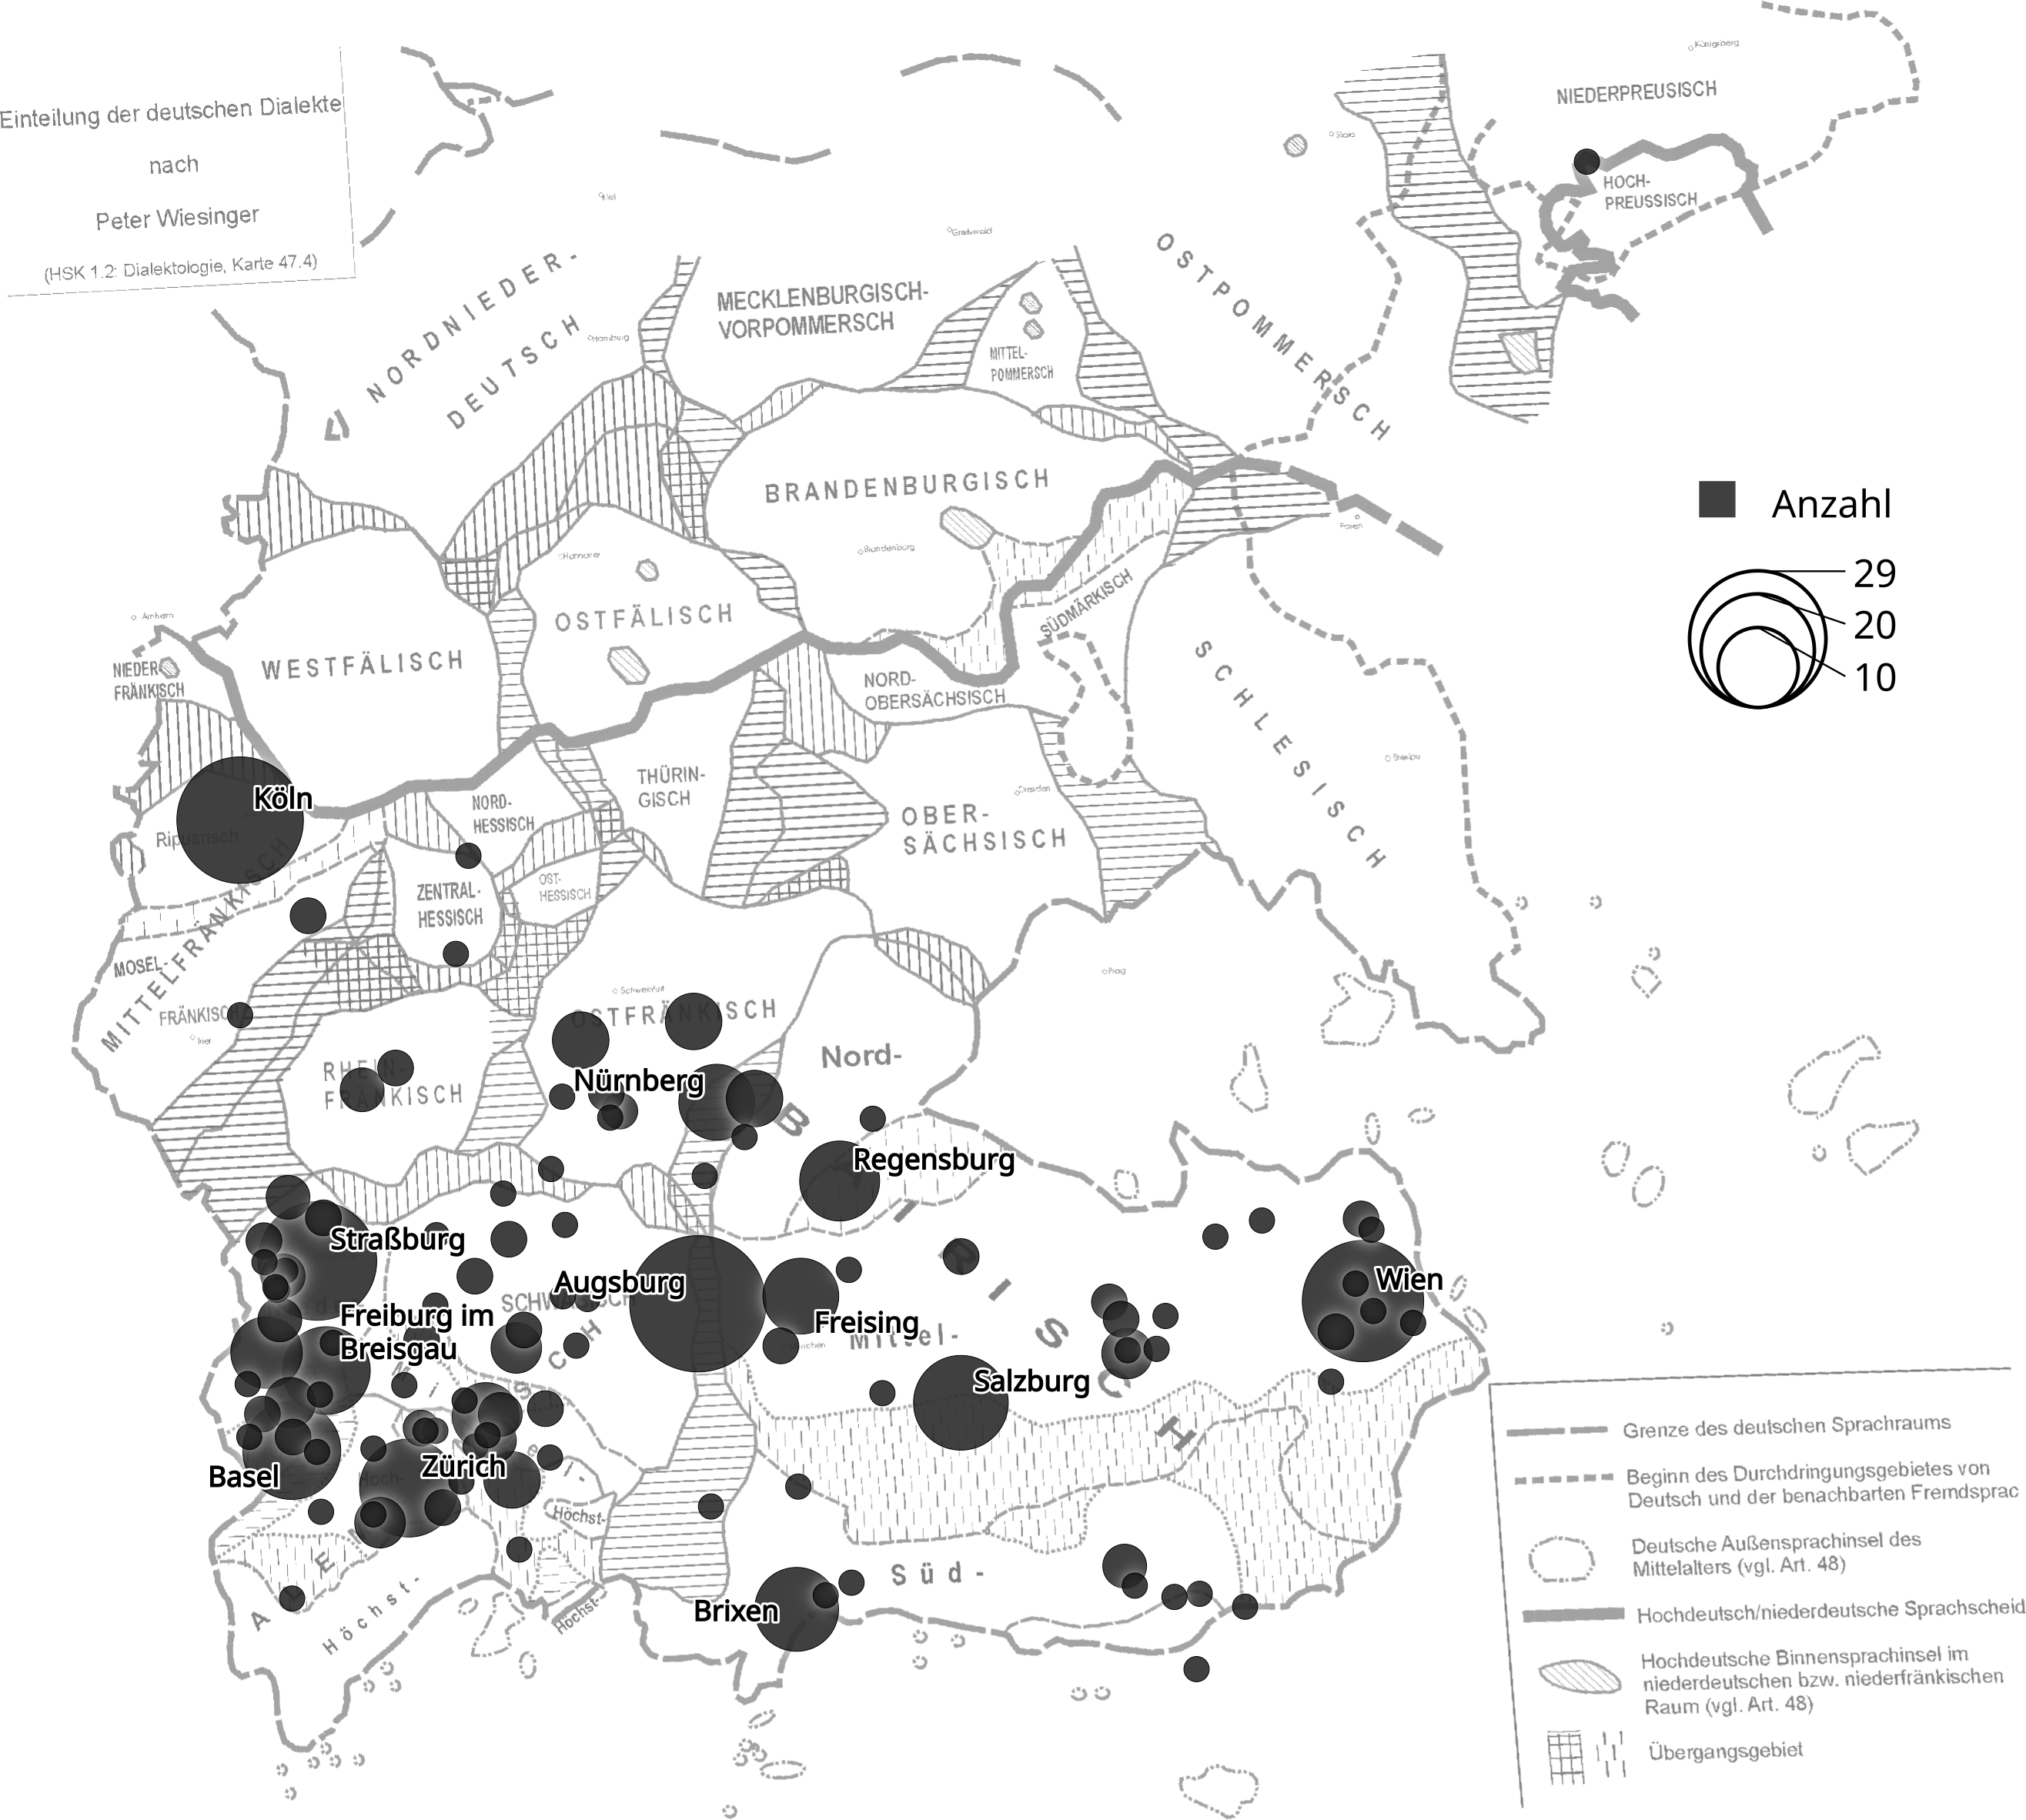
\includegraphics[
	width=\linewidth,
	height=.75\textheight,
	keepaspectratio
]{./assets/grafiken/2021-05-11_cao_beide_iu-per-place-quant+conj.png}
\caption{Anzahl der Belege für mhd.\ \norm{bėide} pro Ausstellungs\-ort
im \citetitle{cao}\nocite{wiesinger1983:rede}}
\label{fig:beidemapcao}
\end{figure}

Die 35 westmitteldeutschen Belege aus Köln (25~Belege), Burg Altleiningen
(Kr.~Bad Dürkheim; 3), Sayn (Kr.~Mayen-Koblenz; 2), Worms (2), Rüdigheim
(Kr.~Marburg-Biedenkopf; 1), Schloss Naumburg (Main-Kinzig-Kreis; 1) und
Veldenz (Kr.~Bernkastel-Wittlich; 1) zeigen den Angaben der Grammatik gemäß
keine Variation zwischen \norm{bėide}- und \norm{bėidiu}-Formen. Diese Belege
werden im weiteren Verlauf von der Analyse ausgeschlossen; die betroffenen
Urkunden werden in \cref{subsec:ausgesurk} aufgeführt. Bei der Besprechung
individueller Belege finden sich im Alemannischen noch weitere Fälle, in denen
am Ort nach kursorischer Durchsicht der Belege für \norm{e}- und
\norm{iu}-Formen in Urkundentexten des jeweiligen Ortes im \citetitle{cao}
keine Variation vorliegt (vgl. auch \cref{sec:adjdeclcao} zu Straßburg). Da
nachfolgend aufgrund der Anzahl der Belege nicht sämtliche von ihnen einzeln
besprochen werden können, ist mit weiteren solchen Fällen gewissermaßen als
\q*{Grundrauschen} zu rechnen.

\needspace{3\baselineskip}
\section{Targets nach Personenmerkmalen des Controllers}
\label{sec:caotargpers}

\subsection{Nominale Controller}
\subsubsection{Kombinierte nominale Controller}
\label{subsubsec:perscombsgnp}

Zunächst werden \norm{bėide} und \norm{bėidiu} in direkter Abhängigkeit von
koordinierten nominalen Ausdrücken (Substantive, Pronomen) wie zum Beispiel
\norm{her Rvͦdiger vnd ſin hovſfrowe} \wdef{Herr Rüdiger und seine Ehefrau} in
\cref{ex:beid2coordncao1} näher betrachtet. Dabei werden Kombinationen von
Personalpronomen und Eigenname wie \norm{ich unde Ulrich} an dieser Stelle
mitgezählt, da auch diese eine nominale Kategorie darstellen, insofern sie
sich im Kontext dieser Untersuchung regelmäßig auf ein substantivisches
Antezedens beziehen und dessen Personenmerkmale reflektieren.
% %
% 	\footnote{Formal ist die Kategorie \xhead{D}, die im Deutschen die Pronomen
% 	enthält, das funktionale Äquivalent zur lexikalischen Kategorie \xhead{N}
% 	der Substantive \autocite[vgl.~z.\,B.][135--138]{bresnanetal2016}.}
% %
Zwei Belege werden in \cref{ex:beid2coordncao1} angeführt. Das beigefügte
Schema verdeutlicht den syntaktischen Kontext.

\begin{exe}
\ex \label{ex:beid2coordncao1}
\begin{xlist}
	\ex \label{ex:beid2coordncao1_1}
		\begin{tikzpicture}[baseline=(1a_lb.base)]
			\node at (0,2)  (1a)    {\norm{her Rvͦdiger}};
			\node           (1a_box)[draw,rectangle,fit=(1a)] {};
			\node           (1a_lb) [above=.5ex of 1a_box, font=\mynodefont]
		                            {Controller 1};

			\node at (0,0)  (1b)    {\norm{ſin hovſfrowe}};
			\node           (1b_box)[draw,rectangle,fit=(1b)] {};
			\node           (1b_lb) [above=.5ex of 1b_box, font=\mynodefont]
		                            {Controller 2};

			\node at (3,1) (2)      {\norm{bediv}};
			\draw (2) node (2_box)  [draw,rectangle,fit=(2)] {};
			\node (2_lb)   [above=.5ex of 2_box, font=\mynodefont] {Target};

			\draw [-latex] (1a_box) to [out=east, in=west] (2_box);
			\draw [-latex] (1b_box) to [out=east, in=west] (2_box);
		\end{tikzpicture}

	\sn \gll swenne aber her \textbf{R\sscr{v}{o}diger} vnd ſin
			\textbf{hovſfrowe} \textbf{bediv} niht enſint\\
			so=wenn aber Herr Rüdiger[\Nom.\Sg.\MascM] und sein
			Ehefrau[\Nom.\Sg.\FemF] beide-\Nom.\Pl.\NeutMF.\St{} nicht
			\Neg=sind\\
			\begin{taggedline}{\parencites(Regensburg, 1299)[\pno~3262, 425.13--14]{cao4}}
			\trans \wdef{Wenn aber irgendwann Herr Rüdiger und seine Ehefrau
				beide nicht \textins{mehr} sind}
			\end{taggedline}

	\ex \label{ex:beid2coordncao1_2}
		\gll Diſ dingeſ gezuga ſint · \textbf{R\sscr{u}{o}d} · von der palma
			min Oͤhen · \textbf{\sscr{v}{o}lrich} von Grvͤnenberch min Oͤhen
			\textbf{bedu} Jungherren \\
			% · hug von waltherſwile · \textelp{} \\
			Dies Verhandlung-\Gen.\Sg.\NeutI{} Zeugen sind {}
			\lit{Ruͦd}[\Nom.\Sg.\MascM] {} von der Palme mein Oheim {}
			Ulrich[\Nom.\Sg.\MascM] von Grünenberg mein Oheim
			beide-\Nom.\Pl.\NeutM.\St{} Jungherren[\Nom.\Pl.\MascM] \\
			% {} Hug von Walterswil {} {} \\
		\begin{taggedline}{\parencites(Kl.~St.~Urban, Kt.~Luzern, 1298)[\pno~2915, 213.33--35]{cao4}}
		\trans \wdef{Zeugen dieser Verhandlung sind: \lit{Ruͦd} von der Palme,
			mein Onkel, Ulrich von Grünenberg, mein Onkel -- beide Junker --
			% Hug von Walterswil, 
			\textelp{}}
		\end{taggedline}
\end{xlist}
\end{exe}

Daneben liegen noch die drei Belege in \cref{ex:beid2coordncao2} vor, die aus
der regulären Auswertung ausgeschlossen wurden, da bei ihnen die Flexion des
Targets vor einem Wort steht, das mit einem Vokal beginnt, also in einer
Hiatusposition steht \autocites[vgl.][90--91]{askedal1973}[191--193,
201]{gjelsten1980}. Dies hat bei den Prosatexten des \citetitle{cao} jedoch
keine große Auswirkung (vgl.~\cref{phsec:caohiatus}), sodass diese Belege
aufgrund der geringen Anzahl zur Analyse hinzugezogen werden können, zumal sie
ansonsten einschlägig sind. In \cref{tab:combnomctrl} erscheinen sie grau
gedruckt.

\begin{exe}
\ex \label{ex:beid2coordncao2}
	\begin{xlist}
	\ex \label{ex:beid2coordncao2_1}
		\gll \textbf{wir} · krafte von hohenloch · vn̄ · \textbf{wir} ludewic
			von durne · geloben \textbf{baide} vf vnſern eit \\
			\Fsg\subM.\Hon.\Nom{} {} Kraft von Hohenlohe {} und {}
			\Fsg\subM.\Hon.\Nom{} Ludwig von Durne {} geloben
			beide-\Nom.\Pl.\MascM.\St{} auf unseren Eid \\
		\begin{taggedline}{\parencites(Burg Hohlach, Kr.~Neustadt an der Aisch-Bad Windsheim)[\pno~2529, 563.5--6]{cao3}}
		\trans \wdef{Wir, Kraft von Hohenlohe, und Wir, Ludwig von Durne,
			geloben beide Kraft unseres Eides}
		\end{taggedline}

	\ex \label{ex:beid2coordncao2_2}
		\gll \textbf{Jch} seibot von freihaim / vnd fraͮwe \textbf{Peters} mein
			Havſfraͮwe / veriehen \textbf{beidev} vnd tuͦn chvnt \\
			\Fsg\subM.\Nom{} Seibot von Freiheim {} und Frau
			Peters[\Nom.\Sg.\FemF] mein Ehefrau {} bekennen
			beide-\Nom.\Pl.\NeutMF.\St{} und tun kund \\
		\begin{taggedline}{\parencites(München, 1299)[\pno~3248, 416.23]{cao4}}
		\trans \wdef{Ich, Seibot von Freiheim, und Frau Peters, meine Ehefrau,
			bekennen beide und machen bekannt}
		\end{taggedline}

	\ex \label{ex:beid2coordncao2_3}
		\gll minen \textbf{hof} \textelp{} verkaufft han mit dem
			\textbf{zehenden} \textelp{}, \textbf{beidev} vnuerſchaidenlichen
			fvͤr reht aigen \\
			meinen Hof[\Acc.\Sg.\MascI] {} verkauft habe mit dem
			Zehnt-\Dat.\Sg.\MascI{} {} beide-\Acc.\Pl.\NeutI.\St{}
			gleichermaßen für rechtmäßig Eigentum \\
		\begin{taggedline}{\parencites(Augsburg, 1283)[\pno~N~241, 195.37--39]{cao5}}
		\trans \wdef{meinen Hof verkauft habe mit dem Zehnten \textelp{}, beide
			gleichermaßen zum rechtmäßigen Eigentum}
		\end{taggedline}
	\end{xlist}
\end{exe}

\cref{tab:combnomctrl} fasst die Personenmerkmale der in
\cref{ex:beid2coordncao1,ex:beid2coordncao2} zitierten Beispiele zusammen und
gibt die Häufigkeiten der jeweiligen Kongruenzformen des Quantors pro
Merkmalskombination an. Zur Angabe der belegten Flexionstypen ist anzumerken,
dass die Spalte \norm{bėidiu} gemäß den Ergebnissen in \cref{sec:adjdeclcao}
zur regionalen Ausprägung von \norm{-e} und \norm{-iu} in der starken
Adjektivdeklination im \citetitle{cao} die verschiedenen als äquivalent
angesehenen Grafien der Flexionsendung zusammenfasst. Dies sind:
\lit{iu/iv},
\lit{îv},
\lit{ivͤ},
\lit{iͤv},
\lit{uͥ/vͥ},
\lit{ú/v́},
\lit{v̓},
\lit{u/v},
\lit{eiw},
\lit{eu/ev}
sowie
\lit{i}.

\begin{table}
\centering
\caption{Flexion nach Personenmerkmalen der kombinierten nominalen Controller}
\begin{tabular}{l l r r}
\toprule
\textbf{Controller 1}
	& \textbf{Controller 2}
	& \textbf{bėide}
	& \textbf{bėidiu}
	\\
\midrule
\Tsg.\MascM      & \Tsg.\MascM       &        & 1        \\
\Tsg.\MascM      & \Tsg.\FemF        &        & 1        \\
\midrule
\mc{2}{l}{Summe}                     &        & 2        \\
\midrule
\midrule
\gr{\Fsg\subM}   & \gr{\Fsg\subM}    & \gr{1} &          \\
\gr{\Fsg\subM}   & \gr{\Tsg.\FemF}   &        & \gr{1}   \\
\gr{\Tsg.\MascI} & \gr{\Tsg.\MascI}  &        & \gr{1}   \\
\midrule
\mc{2}{l}{\gr{Summe}}                & \gr{1} & \gr{2}   \\
\bottomrule
\end{tabular}
\label{tab:combnomctrl}
\end{table}

Die niedrige Belegzahl in \cref{tab:combnomctrl} erweckt den Eindruck, dass die
direkte Modifikation zweier Konjunkte durch \norm{bėide} an sich sehr
selten vorkommt. Unter den regulär gewerteten Belegen aus
\cref{ex:beid2coordncao1} liegt jeweils ein Fall mit gleichem Geschlecht der
Controller und einer mit gemischtem vor; in beiden Fällen steht eine Form vom
Typ \norm{bėidiu}. Nimmt man noch die grau gedruckten Belege aus
\cref{ex:beid2coordncao2} hinzu, bei denen die Flexionsendung im Hiatus steht,
kommt bei belebten Controllern bei gleichem Geschlecht ein Beleg für \norm{-e},
bei verschiedenem Geschlecht ein Beleg für \norm{-iu}, und bei unbelebten
Controllern mit gleichem Genus ebenfalls ein Beleg für \norm{-iu} hinzu.

Auch wenn die Belegzahl hier gering ist, fügen sich die vorhandenen Belege in
die Erkenntnisse der vorliegenden Untersuchung ein:
\textcites[39--40]{behaghel1928}[118]{dal2014} stellen fest, dass besonders im
Zusammenhang mit zwei belebten Nominalphrasen (NPs) mit unterschiedlichem Genus
die morphologisch neutrale Kongruenzform mit \norm{-iu} auftritt.

\phantomsection
\label{phsec:jungherren}
Daneben merkt \textcite[384]{paul2007} an, dass die Möglichkeit besteht, dass
auch zwei Substantive mit gleichem Genus durch
\norm{bėidiu} aufgenommen werden können. Dies ist der Fall im oben unter
\cref{ex:beid2coordncao1_2} zitierten Beleg, der hier vorsichtig so
interpretiert wird, dass sich \lit{bedu} \wdef{beide} in pronominaler Verwendung
gleichzeitig auf Rüdiger und Ulrich bezieht. Die Urkunde \citet[2915]{cao4},
die den Beleg enthält, stammt aus dem alemannischen Sprachraum (Kloster
St.~Urban, Kt.~Luzern; hochalemannisch). Mit
\norm{iu}-Markierung tritt neben dem in \cref{ex:beid2coordncao1_2} zitierten
Beleg nur noch \lit{endru guͦt} \wdef{andere Güter (\Nom.\Pl.\NeutI)}
\autocite[\pno~2915, 213.27]{cao4} auf. Auch wenn \lit{bedu Jungherren}
\wdef{beide Junker} eine eigene Einheit mit Bezug auf zwei nicht namentlich
genannte Personen in der Zeugenliste bilden sollte, wäre die neutrale Form
\lit{bedu} in Bezug auf maskulin-männliches \lit{Jungherren} immer noch
auffällig.

\subsubsection{Einfache nominale Plural-Controller}
\label{subsubsec:persplnp}

Als Vergleichsmaterial zu den Belegen in \cref{subsubsec:perscombsgnp} mit
unmittelbarem Bezug auf koordinierte Controller wurden hier solche
aufgenommen, in denen sich \norm{bėide} direkt auf ein einzelnes Substantiv im
Plural bezieht. Für diesen Kontext gibt es weit mehr Belege, als dass jeder
einzelne zitiert werden könnte. Das Beispiel in \cref{ex:beid2snglncao} dient
zur Illustration.

\begin{exe}
\needspace{5\baselineskip}
\ex \label{ex:beid2snglncao}
	\begin{tikzpicture}[baseline=(1_lb.base)]
		\node at (0,0) (1)    {\lit{wingarten}};
		\node          (1_box)[draw,rectangle,fit=(1)] {};
		\node          (1_lb) [above=.5ex of 1_box, font=\mynodefont]
	                          {Controller};

		\node at (3,0) (2)      {\lit{bede}};
		\draw (2) node (2_box)  [draw,rectangle,fit=(2)] {};
		\node (2_lb)   [above=.5ex of 2_box, font=\mynodefont] {Target};
		
		\draw [-latex] (1_box) to [out=east, in=west] (2_box);
	\end{tikzpicture} \\

\sn \gll ſo mag er wol / die \textbf{bede} \textbf{wingarten} \textelp{}
			verkoͮfen \\
		so kann er wohl {} die beide-\Acc.\Pl.\MascI.\St{}
			Weingarten-\Acc.\Pl.\MascI{} {} verkaufen \\
	\begin{taggedline}{\parencites(Zürich, 1290)[\pno~1221, 484.9]{cao2}}
		\trans \wdef{so kann er wohl die beiden Weingärten \textelp{} verkaufen}
	\end{taggedline}
\end{exe}

\cref{tab:simpnomctrl} bietet eine Übersicht der Verteilung der verschiedenen
Kongruenz\-formen von \norm{bėide} in Abhängigkeit von den
Personenmerkmalen des jeweiligen Controllers.

\begin{table}
\centering
\caption{Flexion nach Personenmerkmalen der einfachen nominalen Controller}
\begin{tabular}{l r r r}
\toprule
\textbf{Controller}
	& \textbf{bėid(e)}
	& \textbf{bėidiu}
	& \textbf{Summe}
	\\
\midrule
\MascM  & 21 &    & 21 \\
\midrule
\MascI  &  7 &    &  7 \\
\NeutI  &  1 &  5 &  6 \\
\midrule
Summe        & 29 &  5 & 34 \\
\bottomrule
\end{tabular}
\label{tab:simpnomctrl}
\end{table}

% \phantomsection
% \label{phsec:herrenchiemsee}
Der eine Beleg für \norm{bėide} in Bezug auf ein Neutrum wird in
\cref{ex:1584_gut} zitiert. Nach der Zuordnung im Ortsverzeichnis
\autocite{cao-online} stammt die Urkunde aus Herrenchiemsee (Kr.~Rosenheim).
Der nächstgelegene Vergleichsort in der Adjektivstichprobe ist München
(vgl.~\cpageref{par:adjmuenchen}). In anderen Urkunden aus Herrenchiemsee und
Umgebung (vornehmlich aus Kloster Altenhohenau, ebenfalls Kr.~Rosenheim) ist
\lit{-iu/eu} als Flexionsform für den Nom./Akk.\ Pl.\ N.\ zumindest bei
Determinierern wie \norm{alliu} \wdef{alle (\N.\Pl)}, \norm{disiu} \wdef{diese
(\N.\Pl)}, oder \norm{unseriu} \wdef{unsere (\N.\Pl)} etabliert.

\begin{exe}
\ex\label{ex:1584_gut}
	\gll ſo ſint \textbf{baide} \textbf{gvt} / dev wiſe / vn̄ freioltzmoſen /
			ledichleichen / dez gotzhauſ datze phaffenwerd \\
		so sind beide-\Nom.\Pl(.\N\subI?).\St{} Gut[\Nom.\Pl.\NeutI] {} die
			Wiese {} und Freiolzmosen {} frei {} des Gotteshaus da=zu
			Pfaffenwerde \\
	\begin{taggedline}{\parencites(Kl.~Herrenchiemsee, Kr.~Rosenheim, 1292)[\pno~1584, 727.26--27]{cao2}}
		\trans \wdef{so stehen beide Güter, die Wiese und Freiolzmosen, dem
		Gotteshaus in Pfaffenwerde zur freien Verfügung}
	\end{taggedline}
\end{exe}

\subsubsection{Zusammenfassung}

Insgesamt ist festzustellen, dass \norm{bėide} mit direktem Bezug auf
nominale Controller im ausgewerteten Urkundenmaterial sehr selten vorkommt. Es
stellt sich die Frage, was der Grund dafür ist. Allgemeingültige Aussagen
lassen sich in jedem Fall angesichts der prekären Beleglage keine machen. Die
Belege passen allerdings zur Beobachtung der einschlägigen Grammatikwerke, dass
in Abhängigkeit von zwei belebten Controllern mit unterschiedlichem Geschlecht
regelmäßig die neutrale Form \norm{bėidiu} auftritt. Daneben tritt
\norm{bėidiu} einmal in Bezug auf zwei Männer auf, was von
\textcite[384]{paul2007} als Möglichkeit zwar angeführt, aber nicht weiter
thematisiert wird.

Bei der Auswertung von \norm{bėide} mit direktem Bezug auf ein
Plural-Substantiv als Controller kommen bei den belebten Controllern nur
männliche Referenten vor; in allen Fällen steht \norm{bėide}. Bei unbelebten
Controllern korrespondiert maskulines Genus regulär mit \norm{bėide}, beim
Neutrum liegt neben regulärem \norm{bėidiu} ebenfalls ein Beleg mit
\norm{bėide} vor.

\subsection{Anaphorische Controller}
\label{subsec:refctrl}

Im letzten Abschnitt zeigte sich, dass im \citetitle{cao}-Belegmaterial
Substantive sehr selten direkte Controller von \norm{bėide} bilden. Der
Großteil der direkten Controller von \norm{bėide} besteht aus verschiedenen
pronominalen Wortarten.
% (%
%	\DRELS,
%	\PPER,
%	\PRF,
%	\DDS,
%	\DPOSA%
% ),
Dies stimmt mit den Beobachtungen von \citet[624--625]{ksw2} überein.

\subsubsection{Indirekter Bezug auf kombinierte nominale Controller}
\label{subsubsec:beid2p2coordncao}

Pronominale Controller wie \wdef{wir} oder \wdef{sie (\Pl)} beziehen sich
bereits auf eine Kombination von Referenten mit ihren jeweiligen
Personenmerkmalen. Das Pronomen ist mit seinem Bezug über den referenziellen
\Index{} verbunden; \norm{bėide} selbst kongruiert mit dem Pronomen. Das
Beispiel in \cref{ex:beid2p2coordncao} verdeutlicht den hier untersuchten
syntaktischen Zusammenhang.%
%
	\footnote{Während für das \q*{klassische} Mhd.\ von einem Unterschied
		zwischen Maskulinum-Femininum \norm{sie} und Neutrum \norm{siu}
		ausgegangen wird \autocites[vgl.][213--214]{paul2007}[369,
		390--397]{ksw2}, fehlt sowohl im \citetitle{cao} als auch in der
		\citet{kc} eindeutige Evidenz für diesen Genusunterschied, vergleiche
		die Teiluntersuchungen zur Form des Pronomens in
		\cref{subsubsec:monoflexioncao}.}

\begin{exe}
\ex\label{ex:beid2p2coordncao}
	\begin{tikzpicture}[baseline=(1a_lb.base)]
		\node at (0,2)  (1a)    [gray]
	                            {\lit{vlreich}};
		\node           (1a_box)[draw,gray,rectangle,fit=(1a)] {};
		\node           (1a_lb) [above=.5ex of 1a_box, gray, font=\mynodefont]
	                            {Controller 1};

		\node at (0,0)  (1b)    [gray]
		                        {\lit{Elzbeten}};
		\node           (1b_box)[draw,gray,rectangle,fit=(1b)] {};
		\node           (1b_lb) [above=.5ex of 1b_box, gray, font=\mynodefont]
	                            {Controller 2};    

		\node at (3,1) (2)      {\lit{ſi}};
		\draw (2) node (2_box1) [
		                    draw,
		                    gray,
		                    minimum height=3em,
		                    minimum width=3em,
		                    xshift=-.5ex,
		                    yshift=+.5ex,
		                    rectangle
		                ] {};
		\draw (2) node (2_box2) [
		                    draw,
		                    minimum height=3em,
		                    minimum width=3em,
		                    xshift=+.5ex,
		                    yshift=-.5ex,
		                    rectangle
		                ] {};
		\node           (2_lb1) [above=.5ex of 2_box1, gray, font=\mynodefont]
		                        {Target};
		\node           (2_lb2) [below=.5ex of 2_box2, font=\mynodefont]
		                        {Controller};

		\node at (6,1)  (3)      {\lit{beidev}};
		\node           (3_box)  [draw,rectangle,fit=(3)] {};
		\node           (3_lb)   [above=.5ex of 3_box, font=\mynodefont]
		                        {Target};

		\draw [-latex,gray] (1a_box) to [out=east, in=west] (2_box1);
		\draw [-latex,gray] (1b_box) to [out=east, in=west] (2_box1);
		\draw [latex-]      (3_box)  to [yshift=1.5ex]      (2_box2);
	\end{tikzpicture}

\sn \gll daz \textbf{vlreich} \textelp{} vor vns hat genomen ze einer
		houſfrowen vrowen \textbf{Elzbeten} \textelp{} vnd \textbf{ſi}
		\textbf{beidev} \textelp{} verzigen habent \textelp{} alles des
		rehtes \\
		dass Ulrich[\Nom.\Sg.\MascM] {} vor uns hat genommen zu einer Ehefrau
		Frau Elisabeth-\Acc.\Sg.\FemF{} {} und \Tpl\subMF{}.\Nom{}
		beide-\Nom.\Pl.\NeutMF.\St{} {} verzichtet haben {} alles des Rechts \\
		\begin{taggedline}{\parencites(Salzburg, 1297)[\pno~2843, 175.22--25]{cao4}}
			\trans \wdef{dass Ulrich \textelp{} vor uns zur Ehefrau
			genommen hat Frau Elisabeth \textelp{} und sie beide \textelp{}
			verzichtet haben auf alles Anrecht}
		\end{taggedline}
\end{exe}

In \cref{tab:caosimprefctrl} geben die Spalten unter \q*{Controller} jeweils
die grammatischen Merkmale des direkten Controllers von \norm{bėide} an:
\Fpl\ entspricht \wdef{wir/uns/unser}, \Tpl\ entspricht \wdef{sie/die/sich}.
Die kombinierten Angaben danach stehen für die Personen\-merkmale der beiden
\q*{Erstcontroller}, das heißt, der nominalen Controller, auf die sich
\norm{bėide} gemäß dem Schema in \cref{ex:beid2p2coordncao} indirekt
bezieht.

\begin{table}
\centering
\caption{Flexion nach Personenmerkmalen der anaphorischen Controller
(kombinierter Bezug)}
\begin{tabular}{
l
%	@{\hspace{4\tabcolsep}}
	l @{$~+~$} l
    r
    @{\hspace{4\tabcolsep}}
    r
    @{\hspace{4\tabcolsep}}
    r
}
\toprule
\mc{3}{c}{\textbf{Controller}}
    & \textbf{bėid(e)}
    & \textbf{bėidiu}
    & \textbf{Summe}
    \\
\midrule
% Controller                     | e  | iu | Σ
\Fpl & \Fsg\subM   & \Fsg\subM   &  4 &    &   4 \\
     & \Fsg\subM   & \Tsg.\MascM &  1 &    &   1 \\

\cmidrule{2-6}

     & \Fsg\subM   & \Fsg\subF   &  1 &  2 &   3 \\
     & \Fsg\subM   & \Tsg.\FemF  &  4 & 12 &  16 \\
     & \Fsg\subF   & \Fsg\subM   &  2 &    &   2 \\
     & \Fsg\subF   & \Tsg.\MascM &  1 &  1 &   2 \\

\midrule

\Tpl & \Tsg.\MascM & \Tsg.\MascM &  6 &    &   6 \\
     & \Tsg.\FemF  & \Tsg.\FemF  &  5 &    &   5 \\

\cmidrule{2-6}

     & \Tsg.\MascM & \Tsg.\FemF  &  9 & 28 &  37 \\
     & \Tsg.\FemF  & \Tsg.\MascM &    &  4 &   4 \\

\cmidrule{2-6}

     & \Tsg.\MascI & \Tsg.\MascI &  2 &  4 &   6 \\
     & \Tsg.\NeutI & \Tsg.\NeutI &    & 23 &  23 \\

\cmidrule{2-6}

     & \Tsg.\MascI & \Tsg.\FemI  &    &  4 &   4 \\
     & \Tsg.\MascI & \Tsg.\NeutI &    &  1 &   1 \\
     & \Tsg.\NeutI & \Tsg.\MascI &    &  1 &   1 \\
     & \Tsg.\NeutI & \Tsg.\FemI  &    &  1 &   1 \\

\midrule

\mc{3}{l}{Summe}                 & 35 & 81 & 116 \\

\midrule
\midrule

\gr{\Tpl} & \gr{\Tsg.\MascM} & \gr{\Tsg.\MascM} & \gr{6} &        &  \gr{6} \\
          & \gr{\Tsg.\FemF}  & \gr{\Tsg.\FemF}  & \gr{2} &        &  \gr{2} \\

\cmidrule{2-6}

          & \gr{\Tsg.\MascM} & \gr{\Tsg.\FemF}  & \gr{2} & \gr{3} &  \gr{5} \\
          & \gr{\Tsg.\FemF}  & \gr{\Tsg.\MascM} &        & \gr{2} &  \gr{2} \\

\cmidrule{2-6}

          & \gr{\Tsg.\NeutI} & \gr{\Tsg.\NeutI} &        & \gr{1} &  \gr{1} \\

\cmidrule{2-6}

          & \gr{\Tsg.\NeutI} & \gr{\Tsg.\MascI} &        & \gr{1} &  \gr{1} \\
          & \gr{\Tsg.\NeutI} & \gr{\Tpl.\MascI} &        & \gr{1} &  \gr{1} \\

\midrule

\mc{3}{l}{\gr{Summe}}                          & \gr{10} & \gr{8} & \gr{18} \\

\bottomrule
\end{tabular}
\label{tab:caosimprefctrl}
\end{table}

\paragraph{Belebt, gleiches Geschlecht}

Die Belege in \cref{tab:caosimprefctrl} für \norm{bėide} mit direktem Bezug
auf Pronomina, die eine Kombination zweier Menschen vom gleichen Geschlecht
repräsentieren, verhalten sich ausgesprochen regelmäßig. In allen Fällen liegt
ein Beleg vom Typ \norm{bėide} vor, in einem Fall in der apokopierten Form
\norm{bėid}, siehe die Beispiele in \cref{ex:cao_samegend_beide}. Was im
Vergleich zu den Belegen mit direktem Bezug auf zwei Substantive mit gleichem
Geschlecht (\cref{subsubsec:perscombsgnp}) nicht bezeugt ist, sind Belege für
\norm{bėidiu} mit indirektem Bezug auf zwei Männer oder Frauen.

\begin{exe}
\ex \label{ex:cao_samegend_beide}
\begin{xlist}
	% \ex \label{ex:cao_samegend_beide_1}
	% 	\gll Wier \textbf{Jacob} vnd \textbf{Hainreich} \textelp{} des geb \textbf{wier} \textbf{baide} diſen brief den {vor genanten} vrowen \\
	% 		Wir Jakob und Heinrich {} dessen geben \Fpl\subM.\Nom{} beide-\Nom.\Pl.\MascM.\St{} diesen Urkunde den vorgenannten Frauen \\
	% 	\begin{taggedline}{\parencite[\pno~N~557, 404.9, 26--27]{cao5}}
	% 	\trans \wdef{Wir, Jakob und Heinrich \textelp{} Deshalb geben wir beide diese Urkunde den vorgenannten Frauen \textelp{von St.~Niklas zu Wien}}
	% 	\end{taggedline}

	\ex \label{ex:cao_samegend_beide_2}
		\gll \textbf{Otten} vnd \textbf{albrehten} von walhen \textelp{} wand
			\textbf{ſi}z \textbf{ped} ziehent an di lande gwizzen \\
			Otto-\Acc.\Sg.\MascM{} und Albrecht-\Acc.\Sg.\MascM{} von Walchen
			{} da \Tpl\subM.\Nom{}=es beide[\Nom.\Pl.\MascM] ziehen an die
			Länder gewiss \\
		\begin{taggedline}{\parencites(Salzburg, 1281)[\pno~491, 431.41, 432.38]{cao1}}
		\trans \wdef{Otto und Albrecht von Walchen \textelp{} da sie es beide
			gewiss (?) \q{an die Lande} ziehen}%
		%
			\footnote{Die Regeste \autocite[80]{caor} erläutert die einzelnen
			Urteile in der Urkunde nicht. Die Übersetzung ist deshalb
			unsicher.}
		%
		\end{taggedline}

	\ex \label{ex:cao_samegend_beide_3}
		\gll sweſter \textbf{Elſbêth} vn sweſter \textbf{Mechthilt} \textelp{} ſo
			\textbf{ſiv} \textbf{beide} tôt ſint \textelp{} \\
			Schwester Elisabeth[\Nom.\Sg.\FemF] und Schwester
			Mechthild[\Nom.\Sg.\FemF] {} so	\Tpl\subF.\Nom{}
			beide-\Nom.\Pl.\FemF.\St{} tot sind {} \\
		\begin{taggedline}{\parencites(Zürich, 1291)[\pno~1504, 679.12--13]{cao2}}
		\trans \wdef{Schwester Elisabeth und Schwester Mechthild \textelp{}
			Wenn sie beide tot sind \textelp{}}
		\end{taggedline}
\end{xlist}
\end{exe}

Zu \cref{ex:cao_samegend_beide_3} ist anzumerken, dass der Beleg aus Zürich und
damit aus dem hochalemannischen Gebiet stammt. Elisabeth und Mechthild werden
für das Alemannische typisch mit \norm{siu} \wdef{sie} bezeichnet. Diese Form
ist nicht als neutral aufzufassen, sondern als genusindifferent aufgrund der
\blockcquote[395]{ksw2}{im Alem.\ wirksamen Tendenz, die neutrale Form
\norm{siu} des Nom./\,Akk.Pl.\ \textelp{} auch auf das Mask.\ und Fem.\
auszudehnen}. Trotzdem zeigt sich in der Stichprobe zu Zürich (siehe
\cpageref{par:adjzuerich}) ein Unterschied zwischen \norm{e}- und
\norm{iu}-Formen in der Deklination von Adjektiven, sodass davon auszugehen ist,
dass es sich hier um einen veritablen Beleg für maskulin-feminines \norm{bėide} in Bezug auf zwei
Frauen handelt.

\paragraph{Belebt, verschiedenes Geschlecht}

Im Gegensatz zu den Belegen im vorigen Absatz liegt bei Targets, die indirekt
von Controllern mit unterschiedlichem Genus beziehungsweise Sexus abhängen,
Variation zwischen \norm{bėide} und \norm{bėidiu} vor. Die Beispiele in
\cref{ex:cao_diffgend_33_beide} stammen \citet{cao-online} zufolge beide aus
Wien (vgl.~\cpageref{par:adjwien}) aus den Jahren 1289 beziehungsweise 1291.

\begin{exe}
\ex \label{ex:cao_diffgend_33_beide}
	\begin{xlist}
	\ex \label{ex:cao_diffgend_33_beide_1}
		\gll Her \textbf{Ernſt} · vnſer burger / vnd ver \textbf{Gerdr\sscr{o}{e}vt} ſein
			hovsvrowe / da \textbf{ſi} \textbf{baide} lebten \\
			Herr Ernst[\Nom.\Sg.\MascM] {} unser Bürger {} und Frau
			Gertrud[\Nom.\Sg.\FemF] sein Ehefrau {} als \Tpl\subMF.\Nom{}
			beide-\Nom.\Pl.\M+\F\subMF.\St{} lebten \\
		\begin{taggedline}{\parencites(Wien, 1289)[\pno~1073, 374.40--41]{cao2}}
		\trans \wdef{Herr Ernst, unser Bürger, und Frau Gertrud, seine Ehefrau,
			als sie beide am Leben waren}
		\end{taggedline}

	\ex \label{ex:cao_diffgend_33_beide_2}
		\gll \textbf{Jch} Heinrich der Swab vnd min houſvrowe \textbf{Chvnegunt}
			\textelp{} {dar vber} geb \textbf{wir} \textbf{paideu} diſen
			prief \\
			\Fsg\subM.\Nom{} Heinrich der Schwab und mein Ehefrau
			Kunigunde[\Nom.\Sg.\FemF] {} darüber geben \Fpl\subMF.\Nom{}
			beide-\Nom.\Pl.\N\subMF.\St{} diesen Urkunde \\
		\begin{taggedline}{\parencites(Wien, 1291)[\pno~N~475, 342.19, 28]{cao5}}
		\trans \wdef{Ich, Heinrich der Schwab, und meine Ehefrau, Kunigunde
			\textelp{} dazu geben wir beide diese Urkunde auf}
		\end{taggedline}
	\end{xlist}
\end{exe}

An der Belegverteilung in \cref{tab:caosimprefctrl} ist zu erkennen, dass unter
den Belegen mit belebter Referenz 80\pct{} der Belege auf die Kombination von
Mann und Frau als Erstcontroller entfallen. Dies ist als Merkmal der
Textsammlung zu werten. Unabhängig von Person und Numerus stehen 17 Belegen für
\norm{bėide} 47 Belege für \norm{bėidiu} gegenüber. Gerade beim
indirekten Bezug auf eine Kombination von dritten Personen unterschiedlichen
Geschlechts (\Tsg.\MascM{} + \Tsg.\FemF, \Tsg.\FemF{} + \Tsg.\MascM; vgl. die
Beispiele in \cref{ex:cao_diffgend_33_beide}) schlägt die Belegzahl mit 32 zu 9
allerdings sehr stark zugunsten von \norm{bėidiu} aus.

Ähnlich verhalten sich die Belegzahlen für den indirekten Bezug auf die
Kombination von erster und dritter Person unterschiedlichen Geschlechts
(\Fsg\subM{} + \Tsg.\FemF, \Fsg\subF{} + \Tsg.\MascM). Auch in diesem
Kontext lässt sich Variation zwischen \norm{bėide} und \norm{bėidiu}
beobachten, wobei das Verhältnis mit 13 zu 5 zugunsten der neutralen Form
ausfällt. Die Beispiele für diesen Kontext in \cref{ex:cao_diffgend_13_beide}
stammen aus
% Basel (1273%
% %; vgl.~\cpageref{par:adjbasel}
% ) und Gebweiler (Guebwiller, Dépt.~Haut-Rhin, 1289) und damit aus
dem niederalemannischen Dialektgebiet.

\begin{exe}
\ex \label{ex:cao_diffgend_13_beide}
	\begin{xlist}
	\ex \label{ex:cao_diffgend_13_beide_1}
		\gll \textbf{Jch} Goͮta \textelp{} do kunt \textelp{} daſ ich mit mineſ
			\textbf{wirteſ} hant \textelp{} Sunderliche heiſſe \textbf{wir}
			\textbf{beide} / den birſelere~\scalebox{.9}{\textelp{}} \\
			\Fsg\subF.\Nom{} Guta {} tue kund {} dass ich mit meines
			Ehemann[\Gen.\Sg.\MascM] Hand {} insbesondere heißen
			\Fpl\subMF.\Nom{} beide-\Nom.\Pl.\M+\F\subMF.\St{} {} den
			Birseler~{} \\
		\begin{taggedline}{\parencites(Basel, 1273)[\pno~199, 210.21--28]{cao1}}
		\trans \wdef{Ich, Guta, \textelp{} mache bekannt \textelp{}, dass ich
			mit der Hand meines Ehemannes \textelp{} Insbesondere heißen wir
			beide den Birseler \textelp{}}
		\end{taggedline}

	\ex \label{ex:cao_diffgend_13_beide_2}
		\gll \textbf{Jch} Rvͦdolf \textelp{} vnde \textbf{Adelheit} min wirtin / tvͤn
			kvnt \textelp{} daſ \textbf{wir} \textbf{beidú} \textelp{} haben
			g̍eg̍eben \textelp{} \\
			\Fsg\subM.\Nom{} Rudolf {} und Adelheid[\Nom.\Sg.\FemF] mein
			Ehefrau {} tun kund {} dass \Fpl\subMF.\Nom{}
			beide-\Nom.\Pl.\NeutMF.\St{} {} haben gegeben {}\\
		\begin{taggedline}{\parencites(Guebwiller, Dépt.~Haut-Rhin, 1289)[\pno~1154, 432.5--11]{cao2}}
		\trans \wdef{Ich, Rudolf \textelp{}, und Adelheid, meine Ehefrau,
			machen bekannt \textelp{}, dass wir beide \textelp{} gegeben haben}
		\end{taggedline}
	\end{xlist}
\end{exe}

Beim indirekten Bezug auf die Kombination von zwei ersten Personen
unterschiedlichen Geschlechts (\Fsg\subM{} + \Fsg\subF, \Fsg\subF{} +
\Fsg\subM) sind die Werte mit drei zu zwei für \norm{bėide} nahezu ausgeglichen,
jedoch ist die Belegzahl zu gering, um dies als eindeutige Tendenz zu werten.
Zwei Belege mit \lit{bede} \wdef{beide (\M+\F?)} und einer mit \norm{bedi}
\wdef{beide (\N?)} stammen ferner aus Straßburg und sind mit Vorsicht zu werten
(vgl.~\cpageref{par:adjstrassburg}). Die Beispiele in
\cref{ex:cao_diffgend_11_beide} % aus Basel (1298%
%; vgl.~\cpageref{par:adjbasel}
% ) und Wien (1295%
%; vgl.~\cpageref{par:adjwien}
% )
illustrieren den Kontext; es handelt sich um die verbleibenden Belege.

\begin{exe}
\ex \label{ex:cao_diffgend_11_beide}
	\begin{xlist}
	\ex \label{ex:cao_diffgend_11_beide_1}
		\gll \textbf{wîr} dú vorgenanten herre \textbf{Otto} / vn fro \textbf{Berchte}
				\textelp{} \textbf{wîr} heîn och \textbf{beîdú} \textelp{}
				gelobet ſtete zehanne \\
			\Fpl\subMF.\Nom{} die vorgenannten Herr Otto[\Nom.\Sg.\MascM] {}
				und Frau Berta[\Nom.\Sg.\FemF] {} \Fpl\subMF.\Nom{} haben
				auch beide-\Nom.\Pl.\NeutMF.\St{} {} versprochen beständig
				zu=haben \\
		\begin{taggedline}{\parencites(Basel, 1298)[\pno~2931, 223.1--6]{cao4}}
		\trans \wdef{Wir, die vorgenannten, Herr Otto und Frau Berta,
		\textelp{} Wir haben auch beide \textelp{} versprochen, beständig zu
			halten}
		\end{taggedline}

	\ex \label{ex:cao_diffgend_11_beide_2}
		\gll \textbf{Wir} loben ovch \textbf{paide}, \textbf{ich} Herman von
			Hipleinſtorf vnd \textbf{ich} Agnes ſein hauſvrowe \textelp{} \\
			\Fpl\subMF.\Nom{} versprechen auch beide-\Nom.\Pl.\M+\F\subMF.\St{}
			\Fsg\subM.\Nom{} Hermann von Hippersdorf und \Fsg\subF.\Nom{}
			Agnes sein Ehefrau {} \\
		\begin{taggedline}{\parencites(Wien, 1295)[\pno~N~701, 506.32--33]{cao5}}
		\trans \wdef{Wir versprechen auch beide, ich, Hermann von
			Hippersdorf, und ich, Agnes, seine Ehefrau, \textelp{}}
		\end{taggedline}
	\end{xlist}
\end{exe}

\phantomsection
\label{phsec:vbctrl}
In einigen Fällen wurden Nullsubjekte als Controller aufgenommen, da im
Teilsatz kein overtes Subjektspronomen vorhanden ist. \norm{Bėide} steht
dennoch an derselben Stelle, die es in der Distanzstellung als Floating
Quantifier (vgl. \cref{sec:floatquant}) einnimmt. Es wird angenommen, dass
\norm{bėide} mit dem Nullsubjekt kongruiert
\autocites[siehe auch][419]{dalrymple2001}[210]{bresnanetal2016}.

\begin{exe}
\ex \label{ex:vvfinctrl}
	\begin{xlist}
	\ex \label{ex:vvfinctrl_1}
		\gll Einen \textbf{garten} vnde einen \textbf{aker} {} ligent
			\textbf{beidú} bi \textelp{} \\			
			einen Garten-\Acc.\Sg.\MascI{}$_i$ und einen
				Acker[\Acc.\Sg.\MascI]$_j$ \Rel$_{i+j}$ liegen
				beide-\Nom.\Pl.\NeutI.\St{}$_{i+j}$ bei {} \\
		\begin{taggedline}{\parencites(Freiburg i.\,Br., 1299)[\pno~3249, 417.4--5]{cao4}}
		\trans \wdef{einen Garten und einen Acker, \textins{die} beide bei
			\textelp{} liegen}
		\end{taggedline}

	\ex \label{ex:vvfinctrl_2}
		\gll \textbf{wir} leben \textelp{} vn̄ {} ſuln daſ ſelbe guͦt
				\textbf{beidú} nieſſen \\				
			\Fpl\subMF.\Nom{}$_i$ leben {} und Ø$_i$ sollen das selbe Gut
				beide-\Nom.\Pl.\NeutMF.\St{}$_i$ nutzen \\
		\begin{taggedline}{\parencites(Neuenburg am Rhein, Kr.~Breisgau-Hochschwarzwald, 1299)[\pno~3376, 493.21--22]{cao4}}
		\trans \wdef{wir leben \textelp{} und \textins{wir} sollen
			dasselbe Gut beide nutzen}
		\end{taggedline}

	\ex \label{ex:vvfinctrl_3}
		\gll \textbf{Jch} Berhtholt vn̄ \textbf{Liebeſte} \textelp{} vn̄
				{} hant das offenliche \textbf{bediv} veriehen
				miteinander \\				
			\Fsg\subM.\Nom{}$_i$ Berthold und Liebeste[\Nom.\Sg.\FemF]$_j$ {}
				und Ø$_{i+j}$ haben das öffentlich
				beide-\Nom.\Pl.\NeutMF.\St{}$_{i+j}$ bezeugt miteinander \\
		\begin{taggedline}{\parencites(Kl.~Niedermünster, Dépt.~Bas-Rhin, 1277)[\pno~N~150, 108.31--32]{cao5}}
		\trans \wdef{Ich, Berthold, und Liebste \textelp{} und \textins{wir}
			haben das öffentlich beide bezeugt miteinander}
		\end{taggedline}

	\ex \label{ex:vvfinctrl_4}
		\gll daſ \textbf{ſie} gewert ſint \textelp{} vn̄ {} hant
				\textbf{bedi} veriehen \\				
			dass \Tpl\subMF.\Nom{}$_i$ gewährt sind {} und Ø$_i$ haben
				beide-\Nom.\Pl.\NeutMF.\St{}$_i$ bezeugt \\
		\begin{taggedline}{\parencites(Straßburg, 1281)[N~202, 156.16]{cao5}}
		\trans \wdef{dass sie bezahlt wurden \textelp{} und \textins{sie} haben
			beide bezeugt}
		\end{taggedline}
	\end{xlist}
\end{exe}

Daneben stehen auch hier zwei Belege, die zunächst aus formalen Gründen aus der
Beleg\-statistik ausgeschlossen wurden, dennoch aber das Phänomen illustrieren.
Auch hier steht \norm{bėide} vor einem Wort, das mit Vokal beginnt.

\begin{exe}
\ex \label{ex:vvfinctrl2}
	\begin{xlist}
	\ex \label{ex:vvfinctrl2_1}
		\gll \textbf{Wir} Otto von Ohſſinſtein / vn̄ Otte der Lantvogt
				\textelp{} vn̄ {} henkent {dar vmbe} \textbf{bêide} vnſer
				Jngeſigel an diſen selben brief \\
			\Tpl\subM.\Nom{}$_i$ Otto von Ochsenstein {} und Otto der Landvogt
				{} und Ø$_i$ hängen darum beide-\Nom.\Pl.\MascM.\St{}$_i$ unser
				Siegel an diesen selben Urkunde \\
		\begin{taggedline}{\parencites(Burg Ochsenstein, Dépt.~Bas-Rhin, 1289)[\pno~1145, 427.5--6]{cao2}}
		\trans \wdef{Wir, Otto von Ochsenstein und Otto der Landvogt \textelp{}
			und \textins{wir} hängen darum beide unser Siegel an diese Urkunde}
		\end{taggedline}

	\ex \label{ex:vvfinctrl2_2}
		\gll \textbf{B˜chart} vn̄ \textbf{C\sscr{v}{o}nrat} von lv̓ſtenowe
				\textelp{} vn̄ {} hant dc \textbf{beide} / ain dem
				adern vor mir {vf gegeben} \\				
			Burkhard$_i$ und Konrad$_j$ von Lustnau {} und Ø$_{i+j}$ haben das
				beide-\Nom.\Pl.\MascM.\St{}$_{i+j}$ {} ein dem andern vor mir
				aufgegeben \\
		\begin{taggedline}{\parencites(Tübingen, 1297)[\pno~2607, 32.41--33.1]{cao4}}
		\trans \wdef{Burkhard und Konrad von Lustnau \textelp{} und
			\textins{sie} haben das beide, einer dem anderen, vor mir
			aufgegeben}
		\end{taggedline}
	\end{xlist}
\end{exe}

\phantomsection
\label{phsec:beidegen}
Während nach \citet[623]{ksw2} regulär nur im Nom./Akk.~Pl.\ mit \norm{bėide}
oder \norm{bėidiu} zu rechnen ist, liegt im ausgewerteten Material darüber
hinaus ein Beleg vor, in dem \norm{bėide} ausnahmsweise im Genitiv auftritt
\cref{ex:1843_kinde}. In \notecite[\pno~1843]{cao3} \autocite{cao3} bezeugt
Ulrich von Wichtrach, das beurkundete Rechtsgeschäft in Einvernehmen mit seiner
Ehefrau Clementine und ihrer beiden Kinder abgewickelt zu haben.

\begin{exe}
\ex\label{ex:1843_kinde}
	% https://www.query.sta.be.ch/detail.aspx?ID=62091
	% Bern, Staatsarchiv des Kantons Bern, Abt. C I a, Stift 1293.11.30
	\gll Jch Vͦlrich \textelp{} kvnde \textelp{} daz ich mit guͦtem rathe
			/ mit miner wirtin \textelp{} vnd vnſer \textbf{beide} kinde hant
			vnd willen \\
		\Fsg\subM.\Nom{} Ulrich {} verkünde {} dass \Fsg\subM.\Nom{} mit gutem
			Rat-\Dat.\Sg{} {} mit \Fsg\subM.\Gen-\Dat.\Sg.\FemF.\St{}
			Ehefrau[\Dat.\Sg.\FemF] {} und \Fpl\subMF.\Gen{} beide-?
			Kind-\Gen.\Pl.\NeutA{} Hand und Willen \\
	\begin{taggedline}{\parencites(Thun, Kt.~Bern, 1293)[\pno~1843, 146.11--13]{cao3}}
	\trans \wdef{Ich, Ulrich, \textelp{} verkünde \textelp{}, dass ich mit
		gutem Rat \textelp{sowie} mit Hand und Willen meiner Ehefrau \textelp{}
		und unser beiden Kinder}
	\end{taggedline}
\end{exe}

Aus dem Text der Urkunde gehen die Namen der Kinder nicht hervor. Die Form
\lit{beide} könnte sich daher entweder auf \lit{vnſer} \wdef{unser} oder auf
\lit{kinde} \wdef{Kinder} beziehen. In beiden Fällen steht unregelmäßig
\norm{bėide} im Gen.\ Pl. Die Korrektheit der Transkription ließ sich anhand
eines Fotos der Original\-urkunde bestätigen (\cref{fig:1843}). Ein
\norm{er}-Haken oder ein Nasalstrich, der die Flexion zu \norm{bėider} oder
\norm{bėiden} machen würde, sind auch im Original nicht vorhanden.
% Das Schriftbild ist regelmäßig und weist nicht auf einen Irrtum des
% Schreibers hin.
Regelmäßiger \fw{n}-Schwund am Wortende \autocite[vgl.][171--172]{weinhold1863}
lässt sich in dieser Urkunde nicht beobachten.

\begin{figure}[h]
\centering

\includegraphics[
	width=\linewidth,
]{./assets/grafiken/CAO_01843_ausschnitt.jpg}
\caption%
	[Ausschnitt aus Bern, Staatsarchiv, StABE~C~I~a, Stift 1293.11.30]%
	{Ausschnitt aus Bern, Staatsarchiv, StABE~C~I~a, Stift 1293.11.30
		\autocites(Foto: Staatsarchiv Bern)[\pno~1843]{cao3}}
\label{fig:1843}
\end{figure}

Der einzige weitere Beleg in einem ähnlichen syntaktischen Kontext wird in
\cref{ex:682_insigel} zitiert. Hier urkunden Abt Volland und Prior Berthold
gemeinsam mit der Klostergemeinschaft. Die Form \lit{bediu} lässt auf Kongruenz
mit \lit{inſigel} \wdef{Siegel} schließen. Der Beleg wurde aufgrund des Hiatus
nicht in \cref{tab:caosimprefctrl} aufgenommen.

\begin{exe}
\ex\label{ex:682_insigel}
	% https://www.wubonline.de/?wub=4267
	% Stuttgart, Hauptstaatsarchiv, A 514 U 50
	\gll Tougen wir abt vollant / vnd Bertholt der prior / vnd der Conuent von
			Hirſowe kunt \textelp{} {dar umbe} haben\footnotemark{}
			wir an dizen breif vnſer \textbf{bediu} inſigel / vnd Grauen
			Aberetheſ von · hohenberc \\
		tun wir Abt Volland[\Nom.\Sg.\MascM] {} und Berthold[\Nom.\Sg.\MascM]
			der Prior {} und der Konvent[\Nom.\Sg.\M\subM] von Hirsau kund {}
			Darum heben \Fpl\subM.\Nom{} an diesen Urkunde
			\Fpl.\Gen.\Pl\subM{} beide-\Acc.\Pl.\NeutI.\St{}
			Siegel[\Acc.\Pl.\NeutI] {} und Graf-\Gen.\Sg{} Albrecht-\Gen{} von
			{} Hohenberg \\
		\begin{taggedline}{\parencites(Kl.~Hirsau, Kr.~Calw, 1284)[\pno~682, 96.3, 11--12]{cao2}}
		\trans \wdef{machen wir, Abt Volland und Berthold der Prior und der
			Konvent von Hirsau bekannt \textelp{} darum hängen wir an diese
			Urkunde unsere beiden Siegel und Graf Albrechts von
			Hohenberg}
		\end{taggedline}
		\footnotetext{Das \citet[780]{wmu1} vermerkt eine
			\textquote{\textins*{g}elegentl.\ Vermengung der Formen von
			\emph{haben} und \emph{heben}}, die auch an dieser Stelle
			anzunehmen ist.}
\end{exe}

Im \citet{rem} finden sich zum Vergleich noch zwei Belege mit \norm{bėide} aus
dem mitteldeutschen Sprachraum, der bei der vorliegenden Untersuchung
ausgeklammert wurde. Die Belege werden in \cref{ex:remgenbeide} zitiert. Die
Annotation ist aus dem \citet{rem} übernommen und in \cref{ex:remgenbeide_1}
unklar. Belege für \norm{bėidiu} im Gen.\ Pl.\ konnten nicht gefunden werden,
das heißt, \lit{-í} in \lit{beidí} ist in \cref{ex:remgenbeide_1} nicht
als Variante von \norm{-iu} zu werten, sondern als ostmitteldeutsche
Schreibweise für \norm{-e} \autocites[52--53]{paul2007}[305]{ksw2}.%
%
	\footnote{
		\begin{tabularx}{\linewidth}[t]{@{} l @{~=~} l @{}}
		M320 &
			\tit{Mühlhäuser Rechtsbuch}
			(Nordhausen, Stadtarchiv, Ms. II, Na 6; \cite[1379]{hsc});
		\\

		M350 & Köln, Historisches Archiv der Stadt, Best.~210 (Domstift), U~3/759 (\DTMdate{1306-09-01}).
		\\
		\end{tabularx}
	}

\begin{exe}
\ex \label{ex:remgenbeide}
\begin{xlist}
	\ex \label{ex:remgenbeide_1}
		\gll von den luitín die vrí beidí gívoren ſien \\
			von den Leuten die ihr-\Gen.\Pl{} beide-\Gen.\Pl{}
			\tsup{?}\norm{gevuore}-\Nom.\Pl.\MascA{} sind
			\\
		\begin{taggedline}{\parencite[\nopp{}M320, 17\vo, 21--22]{rem}}
		% M320 = 'Mühlhäuser Rechtsbuch' (Nordhausen, Stadtarchiv, Ms. II,
		% Na 6; HSC 1379)
		\trans \wdef{von den Leuten, die ihr beider Fahrtgenossen (?) sind}
		\end{taggedline}

	\ex \label{ex:remgenbeide_2}
		\gll van dode der kindˢe beide of irre eyn \\
			von Tod-\Dat.\Sg{} der Kind-\Gen.\Pl{} beide-\Gen.\Pl.\St{} oder
			ihrer ein \\
		\begin{taggedline}{\parencite[\nopp{}M350, 5, 11]{rem}}
		\trans \wdef{durch den Tod beider Kinder oder eines von ihnen}
		\end{taggedline}
\end{xlist}
\end{exe}

\paragraph{Unbelebt, gleiches Genus}

Bei Belegen für \norm{bėide} mit indirektem Bezug auf unbelebte kombinierte
Erstcontroller mit gleichem Genus ergibt sich in \cref{tab:caosimprefctrl} ein
Spiegelbild zum belebten Gegenstück. Neben 23 Fällen von \norm{bėidiu} mit
neutralem Bezug ist die neutrale Form auch in vier von sechs Fällen mit
kombiniertem maskulinem Bezug zu finden \cref{ex:cao_samegend_inan_mm_beidiu}.
Belege für die Kombination zweier unbelebter Feminina sind im ausgewerteten
Material keine vorhanden.

\begin{exe}
\ex \label{ex:cao_samegend_inan_mm_beidiu}
	\begin{xlist}
	\ex \label{ex:cao_samegend_inan_mm_beidiu_1}
		\gll vnſerne \textbf{zehenden} zeandeluingen vnde ainen \textbf{Garten}
				\textelp{} \textbf{div} wier \textbf{baidiv} fvr reht aigen her
				haigen~\textins{sic} braht \\
			unseren Zehnt-\Acc.\Sg{}.\MascI{} zu=Andelfingen und einen
				Garten-\Acc.\Sg.\MascI{} {} \Rel.\Acc.\Pl.\NeutI{} wir
				beide-\Acc.\Pl{}.\NeutI.\St{} für rechtmäßig Eigentum her haben
				gebracht \\
		\begin{taggedline}{\parencites(Kl.~Heiligkreuztal, Kr.~Biberach, 1290)[\pno~1201~AB, 472.10--18]{cao2}}
		\trans \wdef{unseren Zehnten zu Andelfingen und einen Garten \textelp{},
			die wir beide als recht\-mäßiges Eigentum hergebracht haben}
		\end{taggedline}

	\ex \label{ex:cao_samegend_inan_mm_beidiu_2}
		\gll Einen \textbf{garten} vnde einen \textbf{aker} {}
				ligent \textbf{beidú} bi \textelp{} Mit allem dem rehte alſ er
				{-- --} \textbf{ſú} \textbf{bedú} von mir hatte \\
			einen Garten-\Acc.\Sg.\MascI{} und einen Acker[\Acc.\Sg.\MascI]
				Ø liegen beide-\Nom.\Pl.\NeutI.\St{} bei {} mit allem dem
				Recht als er {} \Tpl.\Acc{} beide-\Acc.\Pl.\NeutI.\St{} von mir
				hatte \\
		\begin{taggedline}{\parencites(Freiburg i.\,Br., 1299)[\pno~3249, 417.4--6]{cao4}}
		\trans \wdef{einen Garten und einen Acker, \textins{die} liegen beide
			bei \textelp{}, mit all dem Recht, wie er sie beide von mir hatte}
		\end{taggedline}
	\end{xlist}
\end{exe}

Der Beleg in \cref{ex:cao_samegend_inan_mm_beidiu_1} -- bis auf kleine
Unterschiede in der Großschreibung sind beide Fassungen identisch -- scheint
auf den ersten Blick ambig bezüglich des Antezedens von \lit{baidiv} zu sein.
Allerdings kann die Lesart mit \lit{wier baidiv} \wdef{wir beide} als Einheit
im Kontext der Urkunde ausgeschlossen werden, da drei Aussteller genannt
werden: die Brüder \lit{wezel vn̄ hainrich wezel vnde Cvͦnrat der Bodemer}
% \wdef{Wezel und Heinrich Wezel und Konrad der Bodemer}
\autocite[\pno~1201~AB, 472.7]{cao2}.

Während sich im Material zum \citetitle{cao} keine kombinierten unbelebten
Feminina finden ließen, lieferte eine kurze Recherche im \citet{rem} die drei
in \cref{ex:beid2p2combrem} zitierten Belege zurück, allerdings stammen zwei
davon aus gereimten Texten.%
%
	\footnote{
		\begin{tabularx}{\linewidth}[t]{@{} l @{~=~} l @{}}
		M317 &
			Hugo von Langenstein: \tit{Martina}
			(Basel, Universitätsbibl.,	Cod. B~VIII~27; \cite[2776]{hsc});
		\\

		M342 &
			Gottfried von Straßburg: \tit{Tristan}
			(München, Bayerische Staatsbibl., Cgm~51; \cite[1286]{hsc});
		\\	

		M401 &
			\tit{Baumgarten geistlicher Herzen}
			(München, Bayerische Staatsbibl., Cgm~6247; \cite[1450]{hsc}).
		\\
		\end{tabularx}

		Die Details zu den exzerpierten Passagen können der Webseite des
		\citet[s.\,u.~detaillierte Textübersicht]{rem} entnommen werden.}
%
Alle drei Belege weisen die neutrale Form \norm{bėidiu} mit Bezug auf
kombinierte unbelebte Feminina auf.

\begin{exe}
\ex \label{ex:beid2p2combrem}
	\begin{xlist}
	\ex \label{ex:beid2p2combrem_1}
		\gll Dˢ ſol dich ſchiere machī bloz \\
			der wird dich sogleich machen nackt \\
	\sn \gll \textbf{Gewaltis} vn̄ der \textbf{eren} \\
			Macht[\Gen.\Sg.\FemI] und der Ruhm[\Gen.\Pl.\FemI] \\
	\sn \gll \textbf{Div} sol er \textbf{beidiv} keren \\
			\Dem.\Acc.\Pl.\NeutI{} wird er beide-\Acc.\Pl.\NeutI.\St{}
			verwandeln \\
	\sn \gll In laſtir menicvalt \\
			in Laster vielfältig \\
		\begin{taggedline}{\parencite[\nopp M317, V.~13020--13023]{rem}}
		\trans \wdef{Der wird dich sogleich entblößen der Macht und des Ruhms.
			Die wird er beide in vielfältige Laster verwandeln.}
		\end{taggedline}

	\ex \label{ex:beid2p2combrem_2}
		\gll daz \textbf{triwe} vn̄ \textbf{ere} werde. \\
			dass Treue[\Nom.\Sg.\FemI] und Ruhm[\Nom.\Sg.\FemI] werde \\
	\sn \gll begraben in die erde. \\
			begraben in die Erde \\
	\sn \gll ſo ligent \textbf{ſi} \textbf{beidiv} hie begraben. \\
			so liegen \Tpl\subI.\Nom{} beide-\Nom.\Pl.\NeutI.\St{} hier
			begraben \\
		\begin{taggedline}{\parencite[\nopp M342, V.~18661--18663]{rem}}
		\trans \wdef{dass Treue und Ruhm werde / begraben in der Erde. / So
			liegen sie beide hier begraben.}
		\end{taggedline}

	\ex \label{ex:beid2p2combrem_3}
		\gll der iſt genant ſineſ vater \textbf{tugent} vn̄ \textbf{wiſheit}
			{da von} ſvln ſínív ſchulcheit\upshape\footnotemark{} \textbf{diſiv}
			\textbf{beidiv} von ím lernen. \\
			der ist genannt seines Vater Tugend[\Nom.\Sg.\FemI] und
			Weisheit[\Nom.\Sg.\FemI] davon sollen seine Schulkind
			diese-\Acc.\Pl.\NeutI.\St{} beide-\Acc.\Pl.\NeutI.\St{} von ihm
			lernen \\
		\begin{taggedline}{\parencite[\nopp M401, Bl.~108\vo, 19--21]{rem}}
		\trans \wdef{der wird genannt Tugend und Weisheit seines Vaters.
			Deshalb sollen seine Schulkinder diese beide von ihm lernen.}
		\end{taggedline}
	\end{xlist}
\end{exe}
%
	\footnotetext{Die Schreibung wurde am Digitalisat der Handschrift
%	(\href{https://mdz-nbn-resolving.de/urn:nbn:de:bvb:12-bsb00104263-7}{urn:nbn:de:bvb:12-bsb00104263-7})
	verifiziert, die Glossierung aus dem \citet{rem} übernommen. Dieselbe
	Textstelle in M405Y (München, Bayerische Staatsbibl., Cgm 183: Bl.~4\vo, 5;
	\cite[9715]{hsc}% ;
% 	\href{https://mdz-nbn-resolving.de/urn:nbn:de:bvb:12-bsb00006141-6}{urn:nbn:de:bvb:12-bsb00006141-6}
	) enthält dafür \lit{ſchvͦl chint} \wdef{Schulkinder} und ebenso \lit{diſiv
	beidiv} \wdef{diese beide (\N)}.}

\paragraph{Unbelebt, verschiedenes Genus}

Die Belege in \cref{tab:caosimprefctrl} für \norm{bėide}-Targets in
Abhängigkeit von unbelebten Erstcontrollern mit unterschiedlichem Genus
verhalten sich noch regelmäßiger als ihr belebtes Gegenstück. Die Beispiele in
\cref{ex:cao_diffgend_inan} illustrieren den hier diskutierten
Kongruenzkontext.

\begin{exe}
\ex \label{ex:cao_diffgend_inan}
	\begin{xlist}
	\ex \label{ex:cao_diffgend_inan_1}
		\gll daz ich auz minem \textbf{hauz} vnd auz miner \textbf{hofſtat}
			\textbf{div} \textbf{bediv} min recht eigen ſint \\
			dass ich aus meinem Haus[\Dat.\Sg.\NeutI] und aus meiner
			Grundstück[\Dat.\Sg.\FemI] \Rel.\Nom.\Pl.\NeutI{}
			beide-\Nom.\Pl.\NeutI.\St{} mein rechtmäßig Eigentum sind \\
		\begin{taggedline}{\parencites(Regensburg, 1290)[\pno~1282, 526.37--38]{cao2}}
		\trans \wdef{dass ich aus meinem Haus und aus meinem Grundstück, die 
			beide mein rechtmäßiges Eigentum sind}
		\end{taggedline}

	\ex \label{ex:cao_diffgend_inan_2}
		\gll an dem \textbf{hofe} da ce Holtzhvſen \textelp{} vnde an der
			\textbf{holtzmark} die ich da han, \textbf{div} \textbf{baidiv} min
			reht aigen waren \\
			an dem Hof-\Dat.\Sg.\MascI{} da zu Holzhausen {} und an der
			Waldstück[\Dat.\Sg.\FemI] \Rel.\Nom.\Sg.\FemI{} ich da habe
			\Rel.\Nom.\Pl.\NeutI{} beide-\Nom.\Pl.\NeutI.\St{} mein
			rechtmäßig Eigentum waren \\
		\begin{taggedline}{\parencites(Augsburg, 1285)[\pno~N~272, 215.30--31]{cao5}}
		\trans \wdef{an dem Hof in Holzhausen \textelp{} und an dem Waldstück,
			das ich da habe, die beide mein rechtmäßiges Eigentum waren}
		\end{taggedline}
	\end{xlist}
\end{exe}

In allen sieben Fällen steht eine Form vom Typ \norm{bėidiu}. Sieben Belege
sind nicht genug, um daraus eine Regel abzuleiten, aber die vorhandenen Belege
fügen sich mit denen zum belebten Kontext zu einem Bild zusammen. Insgesamt ist
auffällig, dass nahezu alle Targets mit unbelebter kombinierter Referenz die
neutrale Kongruenzform \norm{bėidiu} aufweisen, unabhängig vom Genus ihrer
Erstcontroller.

\subsubsection{Indirekter Bezug auf unkombinierte Plural-Controller}
\label{subsubsec:beid2p2snglncao}

Zuletzt bleiben noch Belege für Targets zu diskutieren, die sich auf einen
pronominalen Controller beziehen, der sich seinerseits auf ein einzelnes
Substantiv im Plural bezieht. Ein Beispiel für diesen syntaktischen Kontext
gibt \cref{ex:beid2p2snglncao}.

\begin{exe}
\ex \label{ex:beid2p2snglncao}
	\begin{tikzpicture}[baseline=(2_lb1.base)]
	    \node at (0,0)  (1)     [gray]
	                            {\lit{wroͮwen}};
	    \node           (1_box) [draw,gray,rectangle,fit=(1)] {};
	    \node           (1_lb)  [above=.5ex of 1_box, gray, font=\mynodefont]
	                            {Controller};

		\node at (3,0) (2)      {\lit{ſi}};
	    \draw (2) node (2_box1) [
	                        draw,
	                        gray,
	                        minimum height=3em,
	                        minimum width=3em,
	                        xshift=-.5ex,
	                        yshift=+.5ex,
	                        rectangle
	                    ] {};
	    \draw (2) node (2_box2) [
	                        draw,
	                        minimum height=3em,
	                        minimum width=3em,
	                        xshift=+.5ex,
	                        yshift=-.5ex,
	                        rectangle
	                    ] {};
	    \node           (2_lb1) [above=.5ex of 2_box1, gray, font=\mynodefont]
	                            {Target};
	    \node           (2_lb2) [below=.5ex of 2_box2, font=\mynodefont]
	                            {Controller};

	    \node at (6,0)  (3)      {\lit{beide}};
	    \node           (3_box)  [draw,rectangle,fit=(3)] {};
	    \node           (3_lb)   [above=.5ex of 3_box, font=\mynodefont]
	                            {Target};

	    \draw [-latex,gray] (1_box)  to [yshift=-1.5ex]     (2_box1);
	    \draw [latex-]      (3_box)  to [yshift=1.5ex]      (2_box2);
	\end{tikzpicture}

\sn \gll vnd ſol ez den zwein \textbf{wr\sscr{o}{v}wen} gen biz an ir beider tot / ſo
		\textbf{ſi} \textbf{beide} nit enſint \textelp{} \\
		und soll es den zwei Frauen-\Dat.\Pl.\FemF{} übergeben bis an ihr
		beider Tod {} wenn \Tpl\subF.\Nom{} beide-\Nom.\Pl.\M+\F\subF.\St{}
		nicht \Neg=sind {} \\
	\begin{taggedline}{\parencites(Sirnau, Kr.~Esslingen, 1297)[\pno~2568, 3.31]{cao4}}
	\trans \wdef{und soll es den zwei Frauen übergeben bis an ihr beider Tod.
		Wenn sie beide nicht \textins{mehr} sind, \textelp{}}
	\end{taggedline}
\end{exe}

Wie zuvor dienen diese Belege als Vergleich für diejenigen mit Bezug auf
kombinierte Erstcontroller. Ihre Verteilung nach den Personenmerkmalen des
Erstcontrollers gibt \cref{tab:caosimprefctrl2} an. Wie auch in
\cref{tab:simpnomctrl}, dort mit direktem Bezug auf ein Substantiv im Plural,
löst beim indirekten Bezug über ein Pronomen maskuline und feminine Referenz
wie erwartet die Kongruenzform \norm{bėide} aus, neutrale Referenz dagegen eine
Form vom Typ \norm{bėidiu}. Belebtheit scheint auch hier keine Rolle zu
spielen, wenn sich die drei Belege für unbelebte Feminina regelmäßig verhalten.

\begin{table}
\centering
\caption{Flexion nach Personenmerkmalen der anaphorischen Controller
(einfacher Bezug)}
\begin{tabular}{
l
%	@{\hspace{4\tabcolsep}}
	l
    r
    r
    r
}
\toprule
\mc{2}{c}{\textbf{Controller}}
    & \textbf{bėid(e)}
    & \textbf{bėidiu}
    & \textbf{Summe}
    \\
\midrule
% Controller     | e  | iu | Σ
\Tpl & \MascM    &  2 &    &  2 \\
     & \FemF     &  3 &    &  3 \\
     & \NeutF    &    &  4 &  4 \\
     & \NeutX    &    &  2 &  2 \\

\cmidrule{2-5}

     & \FemI     &  3 &    &  3 \\

\midrule

\mc{2}{l}{Summe} &  8 &  6 & 14 \\

\bottomrule
\end{tabular}
\label{tab:caosimprefctrl2}
\end{table}

Im Fall der Formen mit \norm{-iu} unterscheidet \cref{tab:caosimprefctrl2}
zwischen dem Bezug auf Neutra mit weiblichem Bezug und solchen mit unbekanntem
Bezug. Auch wenn die resultierende Kongruenz\-form in beiden Fällen die gleiche
ist, möchte ich die Belege kurz charakterisieren. Die Belege für ersteren
Kontext werden in \cref{ex:cao_beidiu_neutfem} zitiert.

\begin{exe}
\ex \label{ex:cao_beidiu_neutfem}
	\begin{xlist}
	\ex \label{ex:cao_beidiu_neutfem_1}
		\gll \textbf{engiltrvt} ir tohtir Vn̄ \textbf{annvn} ir thohtir thohtir
			\textelp{} ſtirpth der {vor genandon} \textbf{kint} eiz \textelp{}
			ſterbin\textbf{z} {\textbf{beidiv} \textelp{}} \\
			Engeltraut ihr Tochter und Anna-\Obl{} ihr Tochter Tochter {}
			stirbt der vorgenannten Kind[\Gen.\Pl.\NeutF] eines {}
			sterben=\Tpl\subF.\Nom{} beide-\Nom.\Pl.\NeutF.\St{} \\
		\begin{taggedline}{\parencites(St.~Gallen, 1284)[\pno~629, 57.24--25]{cao2}}
		\trans \wdef{Engeltraut, ihre Tochter, und Anna, ihrer Tochter Tochter
			\textelp{} stirbt der vorgenannten Kinder eines \textelp{}
			Sterben sie beide \textelp{}}
		\end{taggedline}

	\ex \label{ex:cao_beidiu_neutfem_2}
		\gll \textbf{Gerhauſe} vnde \textbf{Diemvde} \textelp{} vnde ſwenne {der ſelben}
			\textbf{chinde} einz ſtirbet \textelp{} die wile \textbf{ſi}
			\textbf{beidiv} lebent \textelp{} vnde daz der \textbf{chinde} einz
			dannoch lebt oder \textbf{ſi} \textbf{beidiv} \\
			Gerhaus-\Dat.\Sg.\FemF{} und Diemut-\Dat.\Sg.\FemF{} {} und so=wenn
			derselben Kind-\Gen.\Pl.\NeutF{} eines stirbt {} die Weile
			\Tpl\subF.\Nom{} beide-\Nom.\Pl.\NeutF.\St{} leben {} und dass der
			Kind-\Gen.\Pl.\NeutF{} eines {dann noch} lebt oder \Tpl\subF.\Nom{}
			beide-\Nom.\Pl.\NeutF.\St{} \\
		\begin{taggedline}{\parencites(Nürnberg, 1297)[\pno~2719, 96.43--97.9]{cao4}}
		\trans \wdef{Gerhaus \textins{sic} und Diemut \textelp{} und wenn
			irgendwann derselben Kinder eines stirbt \textelp{} Während sie
			beide am Leben sind \textelp{} und dass der Kinder eines dann
			noch lebt oder sie beide \textelp{}}
		\end{taggedline}

	\ex \label{ex:cao_beidiu_neutfem_3}
		\gll ſweſter \textbf{Gerdrauden} vnd ſweſter \textbf{Diemvden} hern wernhereſ
			\textbf{chinden} \textelp{} vnd ſwenne der vorbenannten \textbf{chinde}
			einez ſtirbet \textelp{} Di weil \textbf{ſi} \textbf{peidev}
			lebent \\
			Schwester Gertraut[\Dat.\Sg.\FemF] und Schwester
			Diemut[\Dat.\Sg.\FemF] Herrn Wernhers Kinder-\Dat.\Pl.\NeutF{} {}
			und so=wenn der vorbenannten Kind-\Gen.\Pl.\NeutF{} eines stirbt
			{} die Weile \Tpl\subF.\Nom{} beide-\Nom.\Pl.\NeutF.\St{} leben \\
		\begin{taggedline}{\parencites(Engelthal, Kr.~Nürnberger Land, 1298)[\pno~2960, 240.31--38]{cao4}}
		\trans \wdef{Schwester Gertraut und Schwester Diemut, Herrn Wernhers
			Kindern \textelp{} Und wenn irgendwann der vorgenannten Kinder eines
			stirbt \textelp{} Während sie beide am Leben sind}
		\end{taggedline}
	\end{xlist}
\end{exe}

Bei allen vier \norm{bėidiu}-Targets geht es um \norm{kint}, also wörtlich
\wdef{Kinder}, wobei dieser Begriff gemäß \citet[\pno~\fw{kint}]{lexer:mhdhwb}
hier treffender in der Bedeutung \wdef{Tochter}
\crefrange{ex:cao_beidiu_neutfem_1}{ex:cao_beidiu_neutfem_3} oder vielleicht
auch spezifischer \wdef{Klosterangehörige}
\crefrange{ex:cao_beidiu_neutfem_2}{ex:cao_beidiu_neutfem_3} aufzufassen ist.
Die \norm{kint} sind dabei im Kontext der Rechtssprache nicht zwangsläufig
minderjährig, insofern Erwachsene unabhängig von ihrem Alter Kinder ihrer
Eltern sind \autocites[vgl.][1736]{schwab2012}[siehe
auch][258--259]{birkenesfleischer2022}. Um welche Personen es sich bei den
\norm{kint} jeweils handelt, geht aus dem Kontext der jeweiligen Urkunden
hervor. Bei \cref{ex:cao_beidiu_neutfem_2,ex:cao_beidiu_neutfem_3} handelt es
sich um die gleichen Personen, die Schwestern Gertraut und Diemut, Töchter des
Wernher vom Stein und Mitglieder des Konvents von Engelthal
\autocite[Kr.~Nürnberger Land; vgl.][619]{caor}.
%
Die Kongruenz zwischen \lit{ſi} und \lit{chinde} \wdef{Kinder} wurde hier
jeweils aufgrund der Nähe zwischen pronominalem Target und nominalem Controller
angenommen. Im ganzen unter\-suchten Material ließen sich keine Belege für
direkte Kongruenz zwischen \norm{bėidiu} und zwei weiblichen Controllern finden%
% , die eine Hypothese über exophorische Kongruenz ermöglichen würden, für
% \norm{bėide} allerdings auch nicht
. Eine Recherche diesbezüglich im
\citet{rem} lieferte keine Ergeb\-nisse.
% , allerdings sind dessen Suchfunktionen zum gegenwärtigen Zeitpunkt nicht
% darauf ausgelegt, komplexe syntaktische Kontexte zu durchsuchen.

Den Beispielen in \cref{ex:cao_beidiu_neutfem} steht der Beleg in
\cref{ex:cao_beidiu_neutunkn} gegenüber. In dieser Urkunde werden die Kinder
nicht beim Namen genannt, allerdings geht der Umstand aus dem Text hervor, dass
zumindest eines von ihnen noch nicht \lit{ze ſinen tagen} \wdef{zu seinen
Tagen} \autocites[\pno~214, 218.18--19]{cao1}[vgl.][26]{caor} gekommen, also
minderjährig ist. Auch hier wurde Kongruenz nach der Form zwischen
\lit{kinden} \wdef{Kindern} und \lit{ſ\sscr{v}{i} beid\sscr{v}{i}} angenommen.

\begin{exe}
\ex \label{ex:cao_beidiu_neutunkn}
	\gll mit zewain \textbf{kinden} \textelp{} daz ſvn \textbf{ſ\sscr{v}{i}}
		\textbf{beid\sscr{v}{i}} han vnze an ir tôt \textelp{} vn̄ ſwen
		\textbf{ſ\sscr{v}{i}} \textbf{beid\sscr{v}{i}} {en ſîn}
		\textelp{} \\
		mit zwei Kind-\Dat.\Pl.\NeutX{} {} das sollen
		\Tpl\tsub{\SX}.\Nom{} beide-\Nom.\Pl.\NeutX.\St{} haben bis an ihr
		Tod {} und so=wenn \Tpl\tsub{\SX}.\Nom{}
		beide-\Nom.\Pl.\NeutX.\St{} \Neg=sind {} \\
	\begin{taggedline}{\parencites(Rottweil, 1274)[\pno~214, 218.17--24]{cao1}}
	\trans \wdef{mit zwei Kindern \textelp{} das sollen sie beide besitzen
		bis an ihren Tod \textelp{} Und wenn sie beide irgendwann nicht
		\textins{mehr} sind \textelp{}}
	\end{taggedline}
\end{exe}

\subsubsection[Zu Askedals (1973) Hypothese der ‚Monoflexion‘]{Zu \posscite{askedal1973} Hypothese der \q*{Monoflexion}}
\label{subsubsec:monoflexioncao}

\citet[99]{askedal1973} stellt bezüglich der Konstruktion \wdef{sie beide} eine
Hypothese zur \q*{Monoflexion} auf. Diese besagt, dass nur eines der beiden
Glieder neutral flektiert würde. Er schließt dies aus der Häufigkeit der Belege
für \norm{die/-iu beide} beziehungsweise \norm{si beide/-iu} in seiner
Stichprobe aus der \citetitle{maroldschroeder1969}-Edition von
\citet{maroldschroeder1969} und der Edition des \citetitle{lachmannhartl1952}
von \citet{lachmannhartl1952}. \cref{tab:asksiebeidekombis} gibt die Ergebnisse
der Auswertung von \citet{askedal1973} wieder; bei den Zahlen in Klammern
\blockcquote[99]{askedal1973}{sind die wahrscheinlichen Elisionsformen mit
einbegriffen}, also Kontexte, in denen der Vokal des Flexionssuffixes im
Hiatus oder am Zeilenende steht.

\begin{table}
\centering
\caption{Kombinationen von \norm{si} und \norm{die/diu} mit \norm{bėide/-iu} \parencite[99]{askedal1973}}
\begin{tabular}{
	l
	r r
	r
	@{\hspace{4\tabcolsep}}
	r r
}
\toprule
\textbf{Controller}
	& \mc{2}{c}{\textbf{bėide}}
	& \textbf{bėidiu}
	& \mc{2}{c}{\textbf{Summe}}
	\\

\midrule

%     | e         | iu | Σ         |
si    &  7 & (14) &  6 & 13 & (20) \\

\midrule

die   &  0 &  (1) &    &  0 &  (1) \\
diu   & \mc{2}{c}{1} &    & \mc{2}{c}{1} \\

\midrule

Summe &  8 & (16) &  6 & 14 & (22) \\
\bottomrule
\end{tabular}
\label{tab:asksiebeidekombis}
\end{table}

In einer Teilauswertung des \citetitle{cao} konnte festgestellt werden, dass in
der Tat \norm{si} die häufigste Form des Pronomens der 3.\ Pers.\ Nom./Akk.\
Pl.\ darstellt. Dies dürfte jedoch weniger der Vermeidung von Redundanz in der
Markierung als vielmehr der Tatsache geschuldet sein, dass sich Ende des
13.~Jahrhunderts der Typ \norm{si} ohne Genusdistinktion als die geläufige
oberdeutsche Form dieses Pronomens etabliert hat. \citet[392, Abb.~P~26]{ksw2} verzeichnen in der zweiten Hälfte des 13.\ Jahrhunderts
für das Bairische, den alemannisch-bairischen Übergangsbereich und das
Alemannische Werte zwischen 96 und 100\pct\ für diesen Typ. Die
\cref{tab:caosiebeidekombis} zeigt die im \citetitle{cao}-Material belegten
Kombinationen und ihre Häufigkeit.

\begin{table}
\centering
\caption{Kombinationen von \norm{si/sie/siu} und \norm{di/die/diu} mit \norm{bėide/-iu} im
\citetitle{cao}}
\begin{tabular}{
	l
	r r
	r
}
\toprule
\textbf{Controller}
	& \textbf{bėid(e)}
	& \textbf{bėidiu}
	& \textbf{Summe}
	\\

\midrule

%     | e  | iu | Σ  |
si    &  8 & 19 & 27 \\
sie   &  3 &  3 &  6 \\
siu   &  5 &  9 & 14 \\

\midrule

di    &  1 &    &  1 \\
die   &  3 &    &  3 \\
diu   &    &  4 &  4 \\

\midrule

Summe & 20 & 35 & 55 \\
\bottomrule
\end{tabular}
\label{tab:caosiebeidekombis}
\end{table}

Eine klare Präferenz für bestimmte Kombinationen ist aus den Daten in
\cref{tab:caosiebeidekombis} nicht herauszulesen. Es bleibt höchstens darauf
hinzuweisen, dass sowohl \norm{sie bėidiu}
% \cref{ex:siebeidiu}
als auch \norm{siu bėide}
%\cref{ex:siubeide}
mehrmals belegt sind. Bei \norm{sie bėidiu} stammen zwei Belege aus dem
bairischen Sprachraum (Rothenburg ob der Tauber, Kloster Stams) und einer aus
dem schwäbischen (Kloster Heiligkreuztal); bei \norm{siu bėide} fanden sich
alle fünf Belege in alemannischen Urkunden (Kloster Kirchberg, Überlingen,
Zürich). Da in keiner der Urkunden, die diese Belege enthalten, ein
systematischer Unterschied zwischen \norm{si}, \norm{sie} und
\norm{siu} festgestellt werden konnte, müssen sie als zum genusneutralen Typ
\norm{si} gehörig gewertet werden.

% \begin{exe}
% \ex \label{ex:siebeidiu}
% 	\gll \textbf{Otto} der Crvͤcær / vn̄ \textbf{willebirk} ſin hvſvrowe \textelp{} die
% 		wile \textbf{ſie} \textbf{baidiv} lebent \\
% 		Otto[\Nom.\Sg.\MascM] der Kreuzer {} und Wilbirg sein Ehefrau {} die
% 		Weile \Tpl\subMF.\Nom{} beide-\Nom.\Pl.\NeutMF.\St{} leben \\
% 	\begin{taggedline}{\autocite[\pno~636, 64.26]{cao2}}
% 	\trans \wdef{Otto der Kreuzer und Wilbirg, seine Ehefrau \textelp{} während
% 		sie beide am Leben sind}
% 	\end{taggedline}

% \ex \label{ex:siubeide}
% \begin{xlist}
% 	\ex \label{ex:siubeide_1}
% 		\gll ... \\
% 			... \\
% 		\begin{taggedline}{\autocite[\pno~1414, 623.26]{cao2}}
% 		\trans \wdef{...}
% 		\end{taggedline}

% 	\ex \label{ex:siubeide_2}
% 		\gll ... \\
% 			... \\
% 		\begin{taggedline}{\autocite[\pno~1504, 679.13]{cao2}}
% 		\trans \wdef{...}
% 		\end{taggedline}
% \end{xlist}
% \end{exe}

Die Belege für \norm{di(e) bėide} und \norm{diu bėidiu} verhalten sich wie
erwartet. Im ersten Fall beziehen sie sich auf Paare aus zwei Männern oder zwei
Frauen, im zweiten auf Paare aus Mann und Frau oder unbelebte Dinge (vgl.
\cref{subsubsec:beid2p2coordncao}).

% \begin{exe}
% \ex \label{ex:diubeidiu}
% 	\begin{xlist}
% 	\ex \label{ex:diubeidiu_1}
% 		\gll ... \\
% 			... \\
% 		\begin{taggedline}{\parencite[\pno~1898, 177.30]{cao3}}
% 		\trans \wdef{}
% 		\end{taggedline}

% 	\ex \label{ex:diubeidiu_2}
% 		\gll ... \\
% 			... \\
% 		\begin{taggedline}{\parencite[\pno~3261, 424.39]{cao4}}
% 		\trans \wdef{}
% 		\end{taggedline}
% 	\end{xlist}
% \end{exe}

\subsubsection{Zusammenfassung und Vergleich}
\label{subsubsec:anaperssum}

Der weitaus größere Teil der Urkundenbelege für \norm{bėide} entfällt auf
Targets mit pro\-nomi\-nalem Controller und damit auf eine bloß indirekte
Abhängigkeit von kombinierten Controllern. Dies bedeutet jedoch nicht, dass
entsprechende weitere Untersuchungen für diesen syntaktischen Zusammenhang
nicht relevant wären, da auch auf Distanz Variation in der Genusmarkierung von
\norm{bėide} als indirektes Target zweier NPs beobachtet werden kann. 
Es konnte nicht festgestellt werden, dass Pronomen, die nicht
nach Genus flektieren, einen neutralisierenden Effekt auf die Form von
\norm{bėide} haben, insofern dass danach immer entweder \norm{bėide} oder \norm{bėidiu} stehen würde.
% Dies lässt sich dadurch begründen, dass auch bei Pronomen ohne morphologische
% Genusmarkierung (\norm{ich}, \norm{wir}, \norm{uns}, \norm{si}, \norm{di})
% auf semantischer Ebene die Koindizierung mit Substantiven steht.

\Cref{tab:cao_e_iu_coord} fasst die Verteilung der Belege für \norm{bėide}
aus \cref{tab:combnomctrl,tab:caosimprefctrl} noch einmal vereinfacht zusammen.
Insgesamt scheint bei der Kongruenzbeziehung zwischen zwei Controllern und
\norm{bėide} ($N_i + N_j$) die Belebtheit der Substantive eine wichtigere
Rolle als deren Genus zu spielen. Aufgrund der geringen Zahl der Belege für den
direkten Bezug auf kombinierte Controller wurden hier die in
\cref{tab:combnomctrl} grau gedruckten Belege mitgezählt, da sie sich nicht
anders verhalten als ihre regulär gezählten Gegenstücke. Aussagen über das
Verhalten des Targets beim direkten Bezug von \norm{bėide} auf zwei unbelebte
Substantive können keine gemacht werden, da dieser Kontext in der Stichprobe
nicht belegt ist.

\begin{table}
\centering
\caption{Flexion nach syntaktischem Kontext (kombinierter Bezug)}
\begin{tabular}{
	l l
	c
	r r
	c
	r r
	c
	r
}
\toprule
\mr{2}{*}{\bfseries Belebtheit}
	& \mr{2}{*}{\bfseries Geschlecht}
	& %
	& \mc{2}{c}{\bfseries $N_i + N_j$}
	& %
	& \mc{2}{c}{\bfseries $PRO_{i + j}$}
	& %
	& \mr{2}{*}{\bfseries Summe}
	\\

\cmidrule{4-5}
\cmidrule{7-8}

%
	& %
	& %
	& \bfseries bėid(e)
	& \bfseries bėidiu
	& %
	& \bfseries bėid(e)
	& \bfseries bėidiu
	& %
	& %
	\\

\midrule

belebt
	& gleich
	& %
	&   1
	&   1
	& %
	&  16
	& 
	& %
	&  18
	\\

%
	& verschieden
	& %
	& 
	&   2
	& %
	&  17
	&  47
	& %
	&  66
	\\

\midrule

unbelebt
	& gleich
	& %
	& 
	&   1
	& %
	&   2
	&  27
	& %
	&  30
	\\

%
	& verschieden
	& %
	& 
	& 
	& %
	& 
	&   7
	& %
	&   7
	\\

\midrule

\mc{2}{l}{Summe}
	& %
	&   1
	&   4
	& %
	&  35
	&  81
	& %
	& 121
	\\

\bottomrule
\end{tabular}
\label{tab:cao_e_iu_coord}
\end{table}

Beim direkten Bezug auf zwei belebte Controller mit verschiedenem Sexus ist nur
\norm{bėidiu} belegt, allerdings mit zwei Belegen nicht sehr häufig. Wesentlich
besser belegt ist der indirekte Bezug von \norm{bėide} auf zwei Erstcontroller
mittels eines Pronomens ($PRO_{i+j}$). Hier liegen für den indirekten Bezug auf
zwei belebte Erstcontroller von gleichem Geschlecht ausschließlich Belege für
\norm{bėide} vor. Beim indirekten Bezug auf zwei belebte Substantive von
unterschiedlichem Geschlecht tritt dagegen Variation zwischen \norm{bėide} und
\norm{bėidiu} auf, wobei die neutrale Form \norm{bėidiu} mehr als doppelt so
häufig vertreten ist.

Beim indirekten Bezug auf kombinierte unbelebte Erstcontroller vom gleichen
Genus entfällt der Großteil der Belege auf \norm{bėidiu} und lediglich zwei auf
\norm{bėide}. Im Fall des indirekten Bezugs auf zwei unbelebte Substantive von
unterschiedlichem Geschlecht ist nur die Form \norm{bėidiu} belegt. Insgesamt
scheint in diesem Kontext also die Form \norm{bėidiu} unabhängig vom Genus
bevorzugt zu werden.

Die Beleglage für den direkten Bezug auf einzelne Plural-Controller wird in
\cref{tab:cao_e_iu_simp} vereinfacht dargestellt, als Quelle dienen die Daten
aus den \cref{tab:simpnomctrl,tab:caosimprefctrl2}. Der Vergleichbarkeit mit
\cref{tab:cao_e_iu_coord} halber wurde auch hier zunächst nach Belebtheit
unterschieden. Die Genera der einzelnen Controller werden jeweils einzeln
aufgeführt, da hier keine Genus-Kombinationen vorliegen. Bei weitem nicht alle
Felder können mit den Belegen aus dem Material des \citetitle{cao} gefüllt
werden. Aufgrund der Lücken lassen sich mit dieser Tabelle allein keine
generellen Aussagen zur Verteilung der \norm{bėide}-Formen mit direktem und
indirekten Bezug auf einzelne Plural-Controller ($N_i$) machen. Die
ausgefüllten Stellen stimmen aber mit dem überein, was nach
\cref{sec:adjdeclcao} regelmäßig zu erwarten ist: Formen vom Typ \norm{bėide}
beschränken sich hauptsächlich auf Kon\-texte mit Bezug auf Maskulina und
Feminina; \norm{bėidiu} ist auf den neutralen Bezug beschränkt. Dies scheint
unabhängig von der Belebtheit und vom syntaktischen Kontext zu gelten.

\begin{table}
\centering
\caption{Flexion nach syntaktischem Kontext (einfacher Bezug)}
\begin{tabular}{
	l l
	c
	r r
	c
	r r
	c
	r
}
\toprule
\mr{2}{*}{\bfseries Belebtheit}
	& \mr{2}{*}{\bfseries Genus}
	& %
	& \mc{2}{c}{\bfseries $N_i$}
	& %
	& \mc{2}{c}{\bfseries $PRO_i$}
	& %
	& \mr{2}{*}{\bfseries Summe}
	\\

\cmidrule{4-5}
\cmidrule{7-8}

%
	& %
	& %
	& \bfseries bėid(e)
	& \bfseries bėidiu
	& %
	& \bfseries bėid(e)
	& \bfseries bėidiu
	& %
	& %
	\\

\midrule

belebt
	& maskulin
	& %
	& 21
	& 
	& %
	&  2
	& 
	& %
	& 23
	\\

%
	& feminin
	& %
	& 
	& 
	& %
	&  3
	& 
	& %
	&  3
	\\

%
	& neutral
	& %
	& 
	& 
	& %
	& 
	&  6
	& %
	&  6
	\\

\midrule

unbelebt
	& maskulin
	& %
	&  7
	& 
	& %
	& 
	& 
	& %
	&  7
	\\

%
	& feminin
	& %
	& 
	& 
	& %
	&  3
	& 
	& %
	&  3
	\\

%
	& neutral
	& %
	&  1
	&  5
	& %
	& 
	& 
	& %
	&  6
	\\

\midrule

\mc{2}{l}{Summe}
	& %
	& 29
	&  5
	& %
	&  8
	&  6
	& %
	& 48
	\\

\bottomrule
\end{tabular}
\label{tab:cao_e_iu_simp}
\end{table}

Beim lexikalischen Blick auf die Kombination \norm{si bėide} hat sich ergeben,
dass -- wie von \citet{askedal1973} für die jeweils verwendeten kritischen
Ausgaben des \tit{Parzival} und des \tit{Tristan} beobachtet -- auch im
\citetitle{cao} mit Abstand die häufigste Variante \norm{si bėide/-iu} ist.
\citeauthor{askedal1973} nimmt an, dass das Fehlen der morphologischen
Markierung von Genus an einem der beiden Glieder grammatikalisiert ist. Eine
Abhängigkeit der Kongruenzform von \norm{bėide} von der Wortform des pronominalen
Controllers konnte im vorliegenden Material jedoch nicht festgestellt werden.
Das umfangreichere Material des \citetitle{cao} weist darüber hinaus mehr
Variation auf als die sehr kleine Stichprobe von \citeauthor{askedal1973}. Die
Häufigkeit von \norm{si} \wdef{sie} ist zumindest im \citetitle{cao} der
Vereinfachung des pronominalen Paradigmas hin zu einer genusübergreifenden
Pluralform zuzuschreiben, die nach \citet[391--392]{ksw2} im Oberdeutschen der
zweiten Hälfte des 13.~Jahrhunderts den Normalfall darstellt \autocite[vgl.\
auch][37--39]{sparmann1961}.

%%%%%%%%%%%%%%%%%%%%%%%%%%%%%%%%%%%%%%%%%%%%%%%%%%%%%%%%%%%%%%%%%%%%%%%%%%%%%%%

\section{Targets nach Distanz zum Controller}
\label{sec:caotargdist}

Die Untersuchungen von \citet{corbett1979} zeigen, dass mit zunehmender Distanz
zwischen Controller und Target die Wahrscheinlichkeit für das Auftreten von
Kongruenz \fw{ad sensum} steigt. Die Distanz lässt sich auf zweierlei Arten
messen: zum einen als linearer Abstand in Wortformen (im Sinne von in sich
geschlossenen morphosyntaktischen Einheiten, vgl.~\cite[252--253]{bauer2000}),
zum anderen als syntaktischer Abstand hinsichtlich der Domäne von Target und
Controller (gleiches Satzglied, gleicher Teilsatz, anderer (Teil-)Satz;
vgl.~\cref{sec:ctrltarg}). Die Beispiele in \cref{fig:caodirdist} verdeutlichen
die jeweilige Zählweise.

\begin{figure}
\centering
\subfloat[Abstand nach Wortformen]{%
	\begin{tikzpicture}[
		baseline=(a.base),
		word/.style={
			draw,
			minimum height=1.5em,
			minimum width=4em,
			font=\itshape
		},
		lbl/.style={
			minimum height=1.5em,
			font={\mynodefont}
		},
		every node/.style={
			anchor=base,
			text height=1.5ex,
			text depth=.5ex
		}
	]

	\node [word]                      (1) {\textbf{Ich}};
	\node [word, base right=1ex of 1] (2) {unde};
	\node [word, base right=1ex of 2] (3) {mīn};
	\node [word, base right=1ex of 3] (4) {\textbf{hūsvrouwe}};
	\node [word, base right=1ex of 4] (5) {verjęhen};
	\node [word, base right=1ex of 5] (6) {\textbf{bėidiu}};

	\path[-]      (1) edge [out=north, in=north] node (a) [lbl, above] {0} (2);
	\path[-]      (2) edge [out=north, in=north] node [lbl, above] {1} (3);
	\path[-]      (3) edge [out=north, in=north] node [lbl, above] {2} (4);
	\path[-]      (4) edge [out=north, in=north] node [lbl, above] {3} (5);
	\path[-latex] (5) edge [out=north, in=north] node [lbl, above] {4} (6);
	\path[-]      (4) edge [out=south, in=south] node [lbl, below] {0} (5);
	\path[-latex] (5) edge [out=south, in=south] node [lbl, below] {1} (6);
	\end{tikzpicture}
	\label{fig:caodirdist_words}
}

\subfloat[Abstand nach der syntaktischen Domäne]{%
 	\begin{tikzpicture}[
		baseline=(vflbl.base),
		box/.style={
			draw,
			minimum height=2.5em,
			font=\itshape
		},
		wordbox/.style={
			draw,
			minimum height=1.75em,
			font=\itshape
		},
		lbl/.style={
			minimum height=1.5em,
			font={\mynodefont}
		},
		every node/.style={
			anchor=base,
			text height=1.5ex,
			text depth=.5ex
		}
	]

	\node [wordbox,                    ] (1) {\textbf{Ich}};
	\node [wordbox, base right=1ex of 1] (2) {unde};
	\node [wordbox, base right=1ex of 2] (3) {mīn};
	\node [wordbox, base right=1ex of 3] (4) {\textbf{hūsvrouwe}};
	\node [wordbox, base right=3ex of 4] (5) {verjęhen};
	\node [wordbox, base right=3ex of 5, thick] (6) {\textbf{bėidiu}};
	\node [         base right=3ex of 6] (7) {\phantom{abcdef}};

	\node (VF)  [box, rectangle, fit={(1) (2) (3) (4)}, thick] {};
	\node (LSK) [box, rectangle, fit=(5)] {};
	\node (MF)  [box, rectangle, fit=(6)] {};
	\node (RSK) [box, rectangle, fit=(7)] {};

	\node (vflbl)  [lbl, above=.5ex of VF]  {VF};
	\node (lsklbl) [lbl, above=.5ex of LSK] {LSK};
	\node (mflbl)  [lbl, above=.5ex of MF]  {MF};
	\node (rsklbl) [lbl, above=.5ex of RSK] {RSK};

	\draw [-, thick] (VF) -- ++(south:2em) -| (6);
	\end{tikzpicture}
	\vspace{.5\baselineskip}
	\label{fig:caodirdist_syn}
}
\caption{Zählweisen bei der Abstandsberechnung}
\label{fig:caodirdist}
\end{figure}

In \cref{fig:caodirdist_words} wird der Abstand zwischen den beiden Controllern
\norm{ich} und \norm{(mīn) hūsvrouwe} \wdef{(meine) Ehefrau} zu ihrem Target
\norm{bėidiu} \wdef{beide} nach Wortformen gezählt. Der erste Sprung zur jeweils
nächsten Wortform wird mit null angesetzt, da zwischen \norm{ich} und
\norm{unde} \wdef{und} sowie zwischen \norm{hūsvrouwe} \wdef{Ehefrau} und
\norm{verjęhen} \wdef{aussagen, bekennen} jeweils kein Abstand besteht. Auf
diese Weise ergibt sich für das Beispiel insgesamt ein kombinierter Wortformenabstand von vier und
eins zwischen Controller und Target.

Bei den Untersuchungen zum Belegmaterial des \citetitle{cao} hat sich die
Entfernungsbestimmung nach Satzgliedern und Sätzen (im Folgenden vereinfachend:
syntaktische Distanz) allerdings als sinnvoller erwiesen. In
\cref{fig:caodirdist_syn} wird das Beispiel der Anschaulichkeit halber
vereinfacht im Rahmen des Feldermodells des deutschen Satzes
\autocites{drach1963}{woellstein2010}[vgl.\ auch][43--51]{mueller2020}
wiederholt. Die Controller \norm{ich} und \norm{hūsvrouwe} \wdef{Ehefrau}
stehen im Vorfeld (VF), während das Target \norm{bėidiu} \wdef{beide} nach der
linken Satzklammer (LSK) im Mittelfeld (MF) steht. Damit steht das Target in
einem anderen Satzteil als seine Controller, dennoch aber im gleichen Teilsatz,
in diesem Fall dem Hauptsatz (\norm{verjęhen} \wdef{aussagen, bekennen} nimmt
in der Regel einen Nebensatz als Komplement). Da die linke Satzklammer mit
einem Vollverb besetzt ist, ist die rechte Satzklammer (RSK) leer. Der
Wortformenabstand steigt tendenziell mit zunehmendem Abstand zwischen
Satzgliedern zueinander und darüber hinaus.

\subsection{Nominale Controller}
\label{subsec:caodistnomctrl}

Für die syntaktische Distanz liegt die in \cref{tab:caocodistp} gezeigte
Belegverteilung vor. Hierbei ist keine Variation in der Lokalität zwischen
beiden Controllern zu beobachten. Es liegen also keine Fälle vor, in denen
beide Controller in unterschiedlichen (Teil-)Sätzen stehen. Aufgrund der
geringen Belegmenge sind auch hier keine starken Konzentrationen von Belegen zu
beobachten. Die unter Vorbehalt aufgenommenen Belege sind grau gedruckt; bei
ihnen handelt es sich in allen Fällen zufällig um Targets in Distanzstellung zu
ihrem Controller (vgl.~\cref{sec:floatquant} zu Floating Quantifiers). In allen
Fällen folgt das Target seinen Controllern.

\begin{table}
\centering
\caption{Flexion nach Distanz von kombinierten nominalen Controllern}
\begin{tabular}{
	l
	c l l
	r
	r
	r
}
\toprule

\textbf{Domäne}
	& \textbf{Wortdist.}
	& \textbf{Controller 1}
	& \textbf{Controller 2}
	& \textbf{bėide}
	& \textbf{bėidiu}
	& \textbf{Summe}
	\\

\midrule

gl.~Satzteil
	& 3 / 0
	& \Tsg.\MascM
	& \Tsg.\FemF
	& %
	& 1
	& 1
	\\

\cmidrule{2-7}

%
	& 7 / 2
	& \Tsg.\MascM
	& \Tsg.\MascM
	& %
	& 1
	& 1
	\\

\midrule

\mc{4}{l}{Summe}
	& 
	& 2
	& 2
	\\

\midrule
\midrule

\gr{gl. Teilsatz}
	& \gr{9 / 3}
	& \gr{\Fsg\subM}
	& \gr{\Tsg.\FemF}
	& %
	& \gr{1}
	& \gr{1}
	\\

\cmidrule{2-7}

%
	& \gr{9 / 4}
	& \gr{\Fsg\subM}
	& \gr{\Fsg\subM}
	& \gr{1}
	& %
	& \gr{1}
	\\

\midrule

\gr{anderer (Teil-)Satz}
	& \gr{20 / 3}
	& \gr{\Tsg.\MascI}
	& \gr{\Tsg.\MascI}
	& %
	& \gr{1}
	& \gr{1}
	\\

\midrule

\mc{4}{l}{\gr{Summe}}
	& \gr{1}
	& \gr{2}
	& \gr{3}
	\\

\bottomrule
\end{tabular}
\label{tab:caocodistp}
\end{table}

Trotz der geringen Belegmenge lässt die Verteilung vermuten, dass
Personenmerkmale eine wichtigere Rolle spielen als die syntaktische Distanz
oder die Distanz nach Wortformen. Einzig der Beleg für zwei unbelebte Maskulina
mit Abstand zwanzig und drei Wortformen fällt durch die unerwartete
\norm{bėidiu}-Form auf. In \cref{subsubsec:beid2p2coordncao} bezüglich des
indirekten Bezugs auf kombinierte Controller konnte jedoch beobachtet werden,
dass bei unbelebtem Bezug häufig auch unab\-hängig vom Genus der Referenten
\norm{bėidiu} steht. Der betreffende Beleg wird in \cref{ex:n241_hofzehnt}
zitiert.

\begin{exe}
\ex\label{ex:n241_hofzehnt}
	\setlength{\glossglue}{5pt plus 2pt minus 1pt}
	\gll daz ich minen frowen von ſande Katerinen minen \textbf{hof}, den ich
		ze Jnningen hete, da etwenne der alte Stevdler ovf ſaz, verkaufft han
		mit dem \textbf{zehenden}, der drovz gat, \textbf{beidev}
		vnuerſchaidenlichen fvͤr reht aigen \\		
		dass ich meinen Frauen von Sankt Katharinen meinen Hof[\Acc.\Sg.\MascI]
		den ich zu Inningen hatte wo vormals der alte Steudler auf saß verkauft
		habe mit dem Zehnt-\Dat.\Sg.\MascI{} der daraus geht
		beide-\Acc.\Pl.\NeutI.\St{} gleichermaßen für rechtmäßig Eigentum \\
	\begin{taggedline}{\parencites(Mainau und Konstanz, 1275)[\pno~N~241, 195.37--38]{cao5}}
	\trans \wdef{dass ich meinen Frauen von St.~Katharinen meinen Hof, den ich
		in Inningen hatte, den vormals der alte Steudler inne hatte, verkauft
		habe \textins{zusammen} mit dem Zehnten, den er einbringt, beide
		gleichermaßen zum rechtmäßigen Eigentum}
	\end{taggedline}
\end{exe}

Wie auch zuvor bleiben noch diejenigen \norm{bėide}-Belege zu diskutieren,
die unmittelbar von einer einfachen NP im Plural abhängen. In allen Fällen
verteilen sich die Formen von \norm{bėide} in
\cref{tab:caopldistpct} wie erwartet. Bei maskulinem Bezug steht \norm{bėide},
bei neutralem in der Regel \norm{bėidiu}. Ob das Target dem Controller
vorangeht oder nachfolgt, hat keine Auswirkung auf die Beleg\-verteilung.

\begin{table}
\centering
\caption{Flexion nach Distanz vom einfachen nominalen Controller}
\begin{tabular}{
	l
	c l
	@{\hspace{4\tabcolsep}}
	r
	r
	@{\hspace{4\tabcolsep}}
	r
}
\toprule

\textbf{Domäne}
	& \textbf{Wortdist.}
	& \textbf{Controller}
	& \textbf{bėid(e)}
	& \textbf{bėidiu}
	& \textbf{Summe}
	\\

\midrule

gl. Satzglied
	& 0 \dots\ 1
	& \MascM
	& 21
	& %
	& 21
	\\

%
	& %
	& \MascI
	& 7
	& %
	& 7
	\\

%
	& %
	& \NeutI
	& 1
	& 3
	& 4
	\\

\midrule

gl. Teilsatz
	& 0 \dots\ 2
	& \Tpl.\NeutI
	& %
	& 2
	& 2
	\\

\midrule

\mc{3}{l}{Summe}
	& 29
	& 5
	& 34
	\\

\bottomrule
\end{tabular}
\label{tab:caopldistpct}
\end{table}

\subsection{Anaphorische Controller}
\label{subsec:caodistanactrl}

Die Frage, wie sich \norm{bėide}-Targets in Bezug auf die Distanz zu
pronominalen Controllern verhalten, lässt sich zweiteilen. Zum einen kann die
Distanz der direkten Abhängigkeit zwischen anaphorischem Controller und Target
untersucht werden, zum anderen kann die Distanz des Pronomens zu seinem
Referenten miteinbezogen werden, also die indirekte Abhängigkeit zwischen den
\q*{Erstcontrollern} und dem \norm{bėide}-Target. Zunächst erfolgt in
\cref{tab:caoanadist} ein Blick auf die direkte Abhängigkeit zwischen
anaphorischem Controller und Target.

\cref{tab:caoanadist} weist die Belegverteilung nach syntaktischem Abstand der
Kongruenzbeziehung aus. Es ist deutlich sichtbar, dass die allermeisten Targets
im gleichen Satzglied wie ihr Controller stehen, und größtenteils in
unmittelbarer Nähe \autocite[vgl.][526--527]{ksw2}. Da aus
\cref{sec:caotargpers} zur Untersuchung der Form des Quantors \norm{bėide}
anhand der referenzierten Personenmerkmale bereits deutlich wurde, dass die
ausschlaggebenden Merkmale für die Variation zwischen \norm{bėide} und
\norm{bėidiu} Belebtheit und gleiches beziehungsweise verschiedenes Geschlecht
(\Sex) beziehungsweise Genus (\Gend) sind, werden in der Tabelle die einzelnen
Targets nicht mehr nach der Feinbestimmung ihrer Personenmerkmale aufgelistet,
sondern nach Belebtheit und gleichem oder verschiedenem Geschlecht
beziehungsweise Genus.

\afterpage{%
\begin{landscape}
\begin{vplace}
\begin{table}
\centering
\caption{Flexion nach Distanz vom anaphorischen Controller (kombinierter
Bezug)}
\begin{tabular}{
	l
	c
	r r c
	r r c
	r r c
	r r
	r
}

\toprule

\mr{3}{*}[-1ex]{\textbf{Domäne}}
	& \mr{3}{*}[-1ex]{\textbf{Wortdist.}}
	& \mc{5}{c}{belebt}
	& %
	& \mc{5}{c}{unbelebt}
	& \mr{3}{*}[-1ex]{\textbf{Summe}}
	\\

\cmidrule{3-7}
\cmidrule{9-13}

%
	& %
	& \mc{2}{c}{gleich}
	& %
	& \mc{2}{c}{verschieden}
	& %
	& \mc{2}{c}{gleich}
	& %
	& \mc{2}{c}{verschieden}
	& %
	\\

\cmidrule{3-4}
\cmidrule{6-7}
\cmidrule{9-10}
\cmidrule{12-13}

%
	& %
	& \mc{1}{c}{\textbf{bėid(e)}}
	& \mc{1}{c}{\textbf{bėidiu}}
	& %
	& \mc{1}{c}{\textbf{bėid(e)}}
	& \mc{1}{c}{\textbf{bėidiu}}
	& %
	& \mc{1}{c}{\textbf{bėid(e)}}
	& \mc{1}{c}{\textbf{bėidiu}}
	& %
	& \mc{1}{c}{\textbf{bėid(e)}}
	& \mc{1}{c}{\textbf{bėidiu}}
	& %
	\\

\midrule

gleiches Satzglied
	& 0--1
	& 10 % belebt gleich beide
	& % belebt gleich beidiu
	& %--
	& 15 % belebt verschieden beide
	& 38 % belebt verschieden beidiu
	& %==
	& % unbelebt gleich beide
	& 1 % unbelebt gleich beidiu
	& %--
	& % unbelebt verschieden beide
	& 2 % unbelebt verschieden beidiu
	& 66 % Summe
	\\

\midrule

gleicher Teilsatz
	& 0--1
	&  6 % belebt gleich beide
	& % belebt gleich beidiu
	& %--
	& % belebt verschieden beide
	&  4 % belebt verschieden beidiu
	& %==
	&  2 % unbelebt gleich beide
	& 26 % unbelebt gleich beidiu
	& %--
	& % unbelebt verschieden beide
	&  5 % unbelebt verschieden beidiu
	& 41 % Summe
	\\

\cmidrule{2-14}

%
	& 2--3
	& % belebt gleich beide
	& % belebt gleich beidiu
	& %--
	&  1 % belebt verschieden beide
	&  4 % belebt verschieden beidiu
	& %==
	& % unbelebt gleich beide
	& % unbelebt gleich beidiu
	& %--
	& % unbelebt verschieden beide
	& % unbelebt verschieden beidiu
	&  5 % Summe
	\\

\cmidrule{2-14}

%
	& 13
	& % belebt gleich beide
	& % belebt gleich beidiu
	& %--
	& % beide belebt verschieden
	&  1 % belebt verschieden beidiu
	& %==
	& % unbelebt gleich beide
	& % unbelebt gleich beidiu
	& %--
	& % unbelebt verschieden beide
	& % unbelebt verschieden beidiu
	&  1 % Summe
	\\

\midrule

\mc{2}{l}{Summe}
	& 16 % belebt gleich beide
	& % belebt gleich beidiu
	& %--
	& 16 % belebt verschieden beide
	& 47 % belebt verschieden beidiu
	& %==
	& 2 % unbelebt gleich beide
	& 27 % unbelebt gleich beidiu
	& %--
	& % unbelebt verschieden beide
	& 7 % unbelebt verschieden beidiu
	& 115 % Summe
	\\

\bottomrule
\end{tabular}
\label{tab:caoanadist}
\end{table}
\end{vplace}
\end{landscape}
}

Bei Targets in der Domäne \q*{gleicher Teilsatz} konzentrieren sich die Belege
auf \norm{bėidiu}. Hierzu ist anzumerken, dass es sich bei 23 dieser Targets
um Quantoren nach Relativpronomen mit kombinierter unbelebter neutraler
Referenz aus Belegen wie dem in \cref{ex:insigel} handelt. Formulierungen
dieser Art sind insbesondere in Augsburger Urkunden sehr häufig anzutreffen und
damit im hier gesammelten Belegmaterial überrepräsentiert.%
%
	\footnote{\citet{haacke1964} hebt die herausragende Rolle des Augsburger
	Stadtschreibers Konrad (nachweisbar von Mitte der 1270er Jahre bis 1285)
	für die Schaffung eines verbindlichen deutschsprachigen Urkundenformulars
	hervor \autocite[111--112]{haacke1964}. Als Merkmal einer Konrad-typischen
	Corroboratio gibt er als Beispiel: \lit{darvmbe han ich im geben diſen
	brief / verſigelt vnde gefeſtent mit minem Jnſigel vnde mit der Stet
	Jnſigel zu auſpurch div baidiv dran hangent} \autocites(Augsburg,
	1285)[120--121]{haacke1964}[vgl.~dazu][\pno~N~272, 216.1--2]{cao5}. Dies
	entspricht im Grunde der Formulierung in \cref{ex:insigel}.}

\begin{exe}
\ex\label{ex:insigel}
	\gll Daz deſ niht vergezzen werde {dar vmb} iſt gemachet dirre brief
			verſigelt vn̄ geveſtent / mit der ſtet \textbf{Jnſigel} ze auſpurch
			/ vn̄ mit vnſerm \textbf{Jnſigel} \textbf{d\sscr{ı}{e}v}
			\textbf{baid\sscr{ı}{e}v} dran hangent \\			
		Dass dessen nicht vergessen werde darum ist gemacht dieser Urkunde
			versiegelt und festgemacht {} mit der Stadt Siegel[\Dat.\Sg.\NeutI]
			zu Augsburg {} und mit unserem Siegel[\Dat.\Sg.\NeutI]
			\Rel.\Nom.\Pl.\NeutI{} beide-\Nom.\Pl.\NeutI.\St{} daran hängen \\
	\needspace{1\baselineskip}
	\begin{taggedline}{\parencites(Augsburg, 1298)[\pno~3056, 304.15--17]{cao4}}
		\wdef{Damit dies nicht vergessen werde, darum ist diese Urkunde
		ausgefertigt versiegelt und bestätigt mit dem Siegel der Stadt
		Augsburg und mit unserem Siegel, die beide daran hängen.}
	\end{taggedline}
\end{exe}

Aus \cref{tab:caoanadist} wird außerdem deutlich, dass weder der Abstand
zwischen Controller und Target in Wortformen noch die syntaktische Distanz
zwischen ihnen einen markanten Einfluss auf die Belegverteilung hat. Auch unter
der Perspektive der Distanz gelten also die Schlussfolgerungen aus
\cref{subsubsec:beid2p2coordncao}. Einzig aufällig ist, dass sich bei der
Distanzstellung von Targets die belebten Belege wesentlich regelmäßiger
entsprechend semantischen Kriterien verhalten als in der Kontaktstellung
(\q*{gleiches Satzglied}). Und zwar steht bei neun von zehn Belegen mit
gemischtgeschlechtlichem Bezug eine Form vom Typ \norm{bėidiu}, während in
Kontaktstellung nur etwa 70\pct{} der Belege auf diese Form entfallen. Beim
unbelebten Bezug dagegen ist kein entsprechender Unterschied zu beobachten.

Betreffend den indirekten Bezug auf einzelne Substantive im Plural als
Erstcontroller gilt dasselbe. Auch hier verteilen sich die fünf Targets in der
Domäne \q*{gleicher Teilsatz} nicht anders als diejenigen in der Domäne
\q*{gleicher Satzteil}. An den bisherigen Beobachtungen zum
Einfluss der Personenmerkmale auf die Form von \norm{bėide} in
\cref{subsubsec:beid2p2snglncao} ändert sich also nichts.

\subsection{Wortformenabstand zu kombinierten Erstcontrollern}

Sehr viele Belege für \norm{bėide} stehen direkt nach einem Pronomen, daher ist
die Aussagekraft der Statistiken im vorhergehenden Abschnitt nicht allzu groß.
Im Folgenden wird daher untersucht, ob die Entfernung zwischen
\norm{bėide}-Targets und ihren \q*{Erstcontrollern} -- also der letzten
expliziten Nennung der nominalen Controller der Kongruenzbeziehung -- einen
Effekt auf die Wahl der Kongruenzform des Targets hat.

Da es für viele Entfernungswerte nur einen einzigen Beleg mit diesem Wert gibt,
ist es sinnvoll, sie zu Klassen zusammenzufassen. Um dem Problem aus dem Weg zu
gehen, gegebenenfalls mit verschiedenen Klassenwerten für die jeweiligen
Erstcontroller arbeiten zu müssen, wurde zur Komplexitätsreduktion bei der
Klassenbildung jeweils das arithmetische Mittel des Wortformenabstands für
jedes Controllerpaar gewertet, vergleiche das fiktive Beispiel in
\cref{tab:worddistarith}.

\begin{table}
\centering
\caption{Beispiel zur Berechnung des gemittelten Wortformenabstands}
\begin{tabular}[t]{c r c c c}
	\toprule
	\textbf{Erstcontroller}
		& \textbf{$\Delta_{Wf}$}
		& \textbf{Controller}
		& \textbf{$\Delta_{Wf}$}
		& \textbf{Target}
		\\

	\midrule

	\norm{Konrad}
		& 47
		& \mr{2}{*}{\norm{si}}
		& \mr{2}{*}{0}
		& \mr{2}{*}{\norm{bėidiu}}
		\\

	\norm{Elisabėth}
		& 43
		& %
		& %
		& %
		\\

	\midrule

	\norm{Konrad}/%
	\norm{Elisabėth}
		& ∅~45
		& \norm{si}
		& 0
		& \norm{bėidiu}
		\\

	\bottomrule
\end{tabular}
\label{tab:worddistarith}
\end{table}

In diesem Beispiel folgt das Kongruenztarget \norm{bėidiu} seinem direkten
Controller \norm{si} unmittelbar, das heißt mit einem Abstand von null
Wortformen. Das Pronomen \norm{si} wiederum geht in letzter Instanz zurück auf
das \q*{Erstcontroller}-Paar \norm{Konrad} und \norm{Elisabėth}. Da zwei
Controller involviert sind, ist deren Abstand zu ihrem pronominalen Target
verschieden: Zwischen \norm{Konrad} und \norm{si} befinden sich 47 Wortformen,
zwischen \norm{Elisabėth} und \norm{si} 43 Wortformen. Um beim Vergleich von
Distanzen nicht ständig mit zwei Werten operieren zu müssen, wird vereinfacht
mit dem gemittelten Abstand zwischen \norm{Konrad} und \norm{Elisabėth} zu
\norm{si} von 45 Wortformen gerechnet. Der Abstand zwischen
\norm{bėidiu} und seinen Erstcontrollern beträgt damit etwa 46 Wortformen.

Die \cref{tab:caodist} stellt die Verteilung der Belege nach Distanzklasse mit
Angabe der durchschnittlichen Distanz zwischen Erstcontrollern und dem
untersuchten Target dar, jeweils nach Belebtheit und gleichem oder
verschiedenem Geschlecht beziehungsweise Genus aufgeteilt. Die gewählte
Einteilung nach vielfachen von Fünferpotenzen mit wachsender Intervallbreite
ist der Praktikabilität geschuldet, insofern sehr wenige Belege in
unmittelbarer Nähe der Erstcontroller vorhanden sind, dafür aber viele im
zweistelligen Bereich. Auch in dieser Darstellung wird deutlich, dass
unabhängig von der linearen Entfernung in Wortformen mit großer Regelmäßigkeit
bei den belebten Targets bei gleichem Geschlecht der Erstcontroller die Form
\norm{bėid(e)} steht, bei unterschiedlichem Geschlecht \norm{bėidiu}. Ebenso
regelmäßig steht bei den unbelebten Targets unabhängig vom Genus der
Erstcontroller \norm{bėidiu}.

\afterpage{%
% \begin{landscape}
% \begin{vplace}
\begin{table}
\centering
\caption{Flexion nach Distanz von kombinierten Erstcontrollern}
%
% {1,2,3,4} × 5 ^ {1,2,3}
%
\begin{tabular}{
	c
	l
	r r c
	r r c
	r r c
	r r
	r
}

\toprule

\mr{3}{*}[-1ex]{\textbf{Klasse}}
	& \mr{3}{*}[-1ex]{\textbf{$\Delta_{Wf}$ (∅)}}
	& \mc{5}{c}{belebt}
	& %
	& \mc{5}{c}{unbelebt}
	& \mr{3}{*}[-1ex]{\textbf{Summe}}
	\\

\cmidrule{3-7}
\cmidrule{9-13}

%
	& %
	& \mc{2}{c}{gleich}
	& %
	& \mc{2}{c}{versch.}
	& %
	& \mc{2}{c}{gleich}
	& %
	& \mc{2}{c}{versch.}
	& %
	\\

\cmidrule{3-4}
\cmidrule{6-7}
\cmidrule{9-10}
\cmidrule{12-13}

%
	& %
	& \mc{1}{c}{\textbf{(e)}}
	& \mc{1}{c}{\textbf{iu}}
	& %
	& \mc{1}{c}{\textbf{(e)}}
	& \mc{1}{c}{\textbf{iu}}
	& %
	& \mc{1}{c}{\textbf{(e)}}
	& \mc{1}{c}{\textbf{iu}}
	& %
	& \mc{1}{c}{\textbf{(e)}}
	& \mc{1}{c}{\textbf{iu}}
	& %
	\\

\midrule

1
	& ≤ 5
	& 5 % belebt gleich beide
	& 1 % belebt gleich beidiu
	& %--
	& % belebt verschieden beide
	& 1 % belebt verschieden beidiu
	& %==
	& 1 % unbelebt gleich beide
	& 18 % unbelebt gleich beidiu
	& %--
	& % unbelebt verschieden beide
	& 3 % unbelebt verschieden beidiu
	& 29
	\\

\midrule

2
	& ≤ 10
	& % belebt gleich beide
	& % belebt gleich beidiu
	& %--
	& 8 % belebt verschieden beide
	& 3 % belebt verschieden beidiu
	& %==
	& 1 % unbelebt gleich beide
	& 6 % unbelebt gleich beidiu
	& %--
	& % unbelebt verschieden beide
	& % unbelebt verschieden beidiu
	& 18
	\\

\midrule

3
	& ≤ 15
	& 2 % belebt gleich beide
	& % belebt gleich beidiu
	& %--
	& % belebt verschieden beide
	& 6 % belebt verschieden beidiu
	& %==
	& % unbelebt gleich beide
	& 2 % unbelebt gleich beidiu
	& %--
	& % unbelebt verschieden beide
	& 1 % unbelebt verschieden beidiu
	& 11
	\\

\midrule

4
	& ≤ 20
	& % belebt gleich beide
	& % belebt gleich beidiu
	& %--
	& 1 % belebt verschieden beide
	& 3 % belebt verschieden beidiu
	& %==
	& % unbelebt gleich beide
	& % unbelebt gleich beidiu
	& %--
	& % unbelebt verschieden beide
	& 1 % unbelebt verschieden beidiu
	& 5
	\\

\midrule

5
	& ≤ 25
	& 2 % belebt gleich beide
	& % belebt gleich beidiu
	& %--
	& % beide belebt verschieden
	& 2 % belebt verschieden beidiu
	& %==
	& % unbelebt gleich beide
	& 1 % unbelebt gleich beidiu
	& %--
	& % unbelebt verschieden beide
	& % unbelebt verschieden beidiu
	& 5
	\\

\midrule

6
	& ≤ 50
	& 2 % belebt gleich beide
	& % belebt gleich beidiu
	& %--
	& 2 % beide belebt verschieden
	& 10 % belebt verschieden beidiu
	& %==
	& % unbelebt gleich beide
	& 1 % unbelebt gleich beidiu
	& %--
	& % unbelebt verschieden beide
	& 1 % unbelebt verschieden beidiu
	& 16
	\\

\midrule

7
	& ≤ 75
	& 1 % belebt gleich beide
	& % belebt gleich beidiu
	& %--
	& % beide belebt verschieden
	& 11 % belebt verschieden beidiu
	& %==
	& % unbelebt gleich beide
	& % unbelebt gleich beidiu
	& %--
	& % unbelebt verschieden beide
	& 1 % unbelebt verschieden beidiu
	& 13
	\\

\midrule

8
	& ≤ 100
	& 1 % belebt gleich beide
	& % belebt gleich beidiu
	& %--
	& 2 % beide belebt verschieden
	& 4 % belebt verschieden beidiu
	& %==
	& % unbelebt gleich beide
	& % unbelebt gleich beidiu
	& %--
	& % unbelebt verschieden beide
	& % unbelebt verschieden beidiu
	& 7
	\\

\midrule

9
	& ≤ 125
	& 1 % belebt gleich beide
	& % belebt gleich beidiu
	& %--
	& % beide belebt verschieden
	& 2 % belebt verschieden beidiu
	& %==
	& % unbelebt gleich beide
	& % unbelebt gleich beidiu
	& %--
	& % unbelebt verschieden beide
	& % unbelebt verschieden beidiu
	& 3
	\\

\midrule

10
	& ≤ 250
	& 2 % belebt gleich beide
	& % belebt gleich beidiu
	& %--
	& 4 % beide belebt verschieden
	& 5 % belebt verschieden beidiu
	& %==
	& % unbelebt gleich beide
	& % unbelebt gleich beidiu
	& %--
	& % unbelebt verschieden beide
	& % unbelebt verschieden beidiu
	& 11
	\\

\midrule

11
	& ≤ 375
	& % belebt gleich beide
	& % belebt gleich beidiu
	& %--
	& % beide belebt verschieden
	& % belebt verschieden beidiu
	& %==
	& % unbelebt gleich beide
	& % unbelebt gleich beidiu
	& %--
	& % unbelebt verschieden beide
	& % unbelebt verschieden beidiu
	& 0
	\\

\midrule

12
	& ≤ 500
	& % belebt gleich beide
	& % belebt gleich beidiu
	& %--
	& % beide belebt verschieden
	& 1 % belebt verschieden beidiu
	& %==
	& % unbelebt gleich beide
	& % unbelebt gleich beidiu
	& %--
	& % unbelebt verschieden beide
	& % unbelebt verschieden beidiu
	& 1
	\\

\midrule

\mc{2}{l}{Summe}
	&  16 % belebt gleich beide
	&   1 % belebt gleich beidiu
	& %--
	&  17 % belebt verschieden beide
	&  48 % belebt verschieden beidiu
	& %==
	&   2 % unbelebt gleich beide
	&  28 % unbelebt gleich beidiu
	& %--
	&   0 % unbelebt verschieden beide
	&   7 % unbelebt verschieden beidiu
	& 119 % Summe
	\\

\bottomrule
\end{tabular}
\label{tab:caodist}
\end{table}
% \end{vplace}
% \end{landscape}
}

Eine auffällige Abweichung besteht bei den Targets mit belebten Erstcontrollern
von verschiedenem Geschlecht in der Distanzklasse 2 (Abstand zwischen 6 und 10
Wortformen). Nahezu drei Viertel der Belege für diesen Kontext zeigen die Form
\norm{bėide}. Im Vergleich zu demselben Kontext in anderen Distanzklassen
liegt also eine umgekehrte Verteilung der Belege vor. Bei allen diesen Belegen
bezieht sich \norm{bėide} auf ein Paar aus Mann und Frau und steht direkt
hinter oder kurz nach einem Personalpronomen in einem anderen Teilsatz als
seine Erstcontroller. Prinzipiell unterscheiden sich die Belege jedoch nicht
von anderen bisher besprochenen. Ein regionaler Cluster ist auch nicht
erkennbar -- die Belege stammen sowohl aus dem mittelbairischen als auch aus
dem hoch- und niederalemannischen Sprachraum.

Ein Anstieg von \norm{bėide}-Targets mit belebter Referenz bei verschiedenem
Geschlecht der Erstcontroller ist auch in der Distanzklasse 10 (Abstand zwischen
126 und 250 Wortformen) zu beobachten. Die Form \norm{bėide} macht hier nahezu
die Hälfte der Belege für diesen Kontext aus. Bei niedrigeren Abständen kommen
dagegen nur vereinzelt Targets vom Typ \norm{bėide} vor. Die Verteilung erweckt
den Eindruck, dass Variation zwischen \norm{bėide} und \norm{bėidiu} besonders
bei eher nahen Targets mit 6 bis 10 Wort\-formen Abstand herrscht, wobei
\norm{bėidiu} ansonsten durchweg die Hauptform darstellt. Der plötzliche
Anstieg der \norm{bėide}-Form bei Targets mit verschiedenem belebten Geschlecht
im oberen Abstandsbereich wird ebenfalls als Zufall gewertet.

\subsection{Zusammenfassung und Vergleich}

Die Belege für \norm{bėide} in direkter Abhängigkeit von Pronomina nach Distanz
zeigen, dass der Großteil der Targets in unmittelbarer Entfernung zu seinem
Controller steht: direkt dahinter und damit in der Regel im gleichen Satzglied
\autocite[vgl.\ auch][625--626]{ksw2}. Der Abstand zwischen Controller und
Target scheint keine Auswirkungen auf die Form des Targets zu haben; vielmehr
variieren die Targets durchweg in Bezug auf die Personenmerkmale ihres
Controllers beziehungsweise ihrer Controller. Auch in Hinblick auf den
Wortformenabstand zwischen \q*{Erstcontrollern} und \norm{bėide}-Targets ändert
sich daran prinzipiell nichts. Damit gelten die Schlüsse, die in
\cref{sec:caotargpers} bezüglich des Einflusses der Kombination von
Personenmerkmalen auf die Form von
\norm{bėide} gezogen wurden, auch unter Berücksichtigung von Wortformenabstand
und syntaktischer Distanz.

Auffällig ist allerdings, dass einerseits \norm{bėide} mit Bezug auf die
Kombination zweier belebter Erstcontroller vom gleichen Geschlecht ($\SM+\SM{}$
und $\SF+\SF$) und andererseits \norm{bėidiu} mit Bezug auf die Kombination
zweier belebter Erstcontroller mit unterschiedlichem Geschlecht ($\SM+\SF$,
$\SF+\SM$) unabhängig von der Distanz dominant ist. Dasselbe gilt für
\norm{bėidiu} in Bezug auf die Kombination unbelebter Controller unabhängig von
deren Genus. Die Vermutung, dass mit wachsendem Abstand die spezifische
Information \q*{Menschen von unterschiedlichem Geschlecht}, die Gender
Resolution bei Targets hin zum Neutrum auslöst, von der unspezifischeren
Information \q*{Menschen} verdrängt wird, hat sich im untersuchten Material
des \citetitle{cao} nicht bestätigt. Es ließ sich also nicht beobachten, dass
\norm{bėide} \wdef{beide (\M+\F)} mit wachsender Distanz zwischen Controller
und Target gegenüber \norm{bėidiu} \wdef{beide (\N)} dominiert.

Es lässt sich trotzdem feststellen, dass im Nahbereich zwischen
durchschnittlich fünf bis neun Wortformen Abstand zwischen Erstcontrollern und
dem jeweils untersuchten Target und wieder im Fernbereich der Klasse 10
(Abstand zwischen 126 und 250 Wortformen) die Form \norm{bėide} verstärkt in
Bezug auf belebte Erstcontroller mit verschiedenem Geschlecht auftritt. In
allen diesen Fällen ist \norm{bėide} indirekt über ein oder mehrere
anaphorische Ausdrücke (Pronomina wie \norm{ich, wir, uns}) mit der letzten
vollständigen Nennung seiner Controller verbunden.

Auch wenn Urkunden mündlich durchgeführte Verhandlungen dokumentieren und sich
vermuten lässt, dass sie gemäß der verbreiteten Formel \norm{hȫren lęsen}
\wdef{lesen hören} darauf ausgelegt sind, mündlich verlesen zu werden
\autocites[595]{schmidtwiegand1998b}[31]{schulze2011}, könnte man den Grund
dafür in konzeptueller Schriftlichkeit suchen. \citet[588--589]{frenz1998b}
zufolge kam es durchaus vor, dass vor Abfassung einer Reinschrift ein
Textentwurf den Urkundenparteien zur Zustimmung vorgelegt wurde. Geübte
Schreiberinnen und Schreiber waren sich bei der Abfassung des Urkundentexts
vermutlich durchgängig um die Zusammensetzung der urkundenden Partei bewusst
und setzten die Kongruenzformen dementsprechend.

% Nr. 2299 (Nürnberg, GNM, Pergamenturkunden, Or. Perg. 1295 Dezember 21,
% http://ha.gnm.de/objekt_start.fau?prj=HA-ifaust&dm=Historisches+Archiv&ref=14033)
% ist glaub ich ziemlich gekritzelt. Tullner Urkunden z.B. sind extrem sauber
% geschrieben

%%%%%%%%%%%%%%%%%%%%%%%%%%%%%%%%%%%%%%%%%%%%%%%%%%%%%%%%%%%%%%%%%%%%%%%%%%%%%%%

\section{\norm{Bėide} als Konjunktion}
\label{sec:caokonjunktion}

Für die Verwendung von \norm{bėide} als Konjunktion ließen sich 157 Belege im
\citetitle{cao}-Material finden. Davon schieden dreißig Belege aus, die
westmitteldeutschen Urkunden entstammen, da in diesem Sprachraum immer die Form
\norm{bėide} steht. Analog zur Auswertung in \cref{sec:adjdeclcao} zur
Adjektivdeklination im \citetitle{cao} gibt \cref{tab:caobeidefuncvar} die
Belegmengen in der Region ausgewählter Ausstellungs\-orte nach Funktion von
\norm{bėide} getrennt wieder. Beim Quantor wurden zum Vergleich nur Kontexte
mit zwei Controllern (direkter und indirekter Bezug) berücksichtigt.

\begin{table}
\centering
\caption{Form von \norm{beide/iu} an exemplarischen Ausstellungsorten nach Funktion}
\begin{tabular}[t]{
	l
	r r
	r r
	r
	c
}
\toprule

\mr[c]{2}{*}{\textbf{Region}}
	& \mc{2}{c}{\textbf{Quantor}}
	& \mc{2}{c}{\textbf{Konjunktion}}
	& \mr[c]{2}{*}{\textbf{Summe}}
	& \mr[c]{2}{*}{\bfseries \makecell[c]{unterschiedl.\\ Verhalten}}
	\\

\cmidrule(rl){2-3}
\cmidrule(rl){4-5}

%
	& \textit{beid(e)}
	& \textit{beidiu}
	& \textit{beid(e)}
	& \textit{beidiu}
	& %
	& %
	\\

\midrule

Straßburg
	&  9
	&  2
	& 13
	&  1
	& 25
	& ---
	\\

Basel
	&  4
	&  6
	&  2
	&  3
	& 15
	& ---
	\\

Zürich
	&  8
	&  4
	&  1
	&  2
	& 15
	& ---
	\\

\midrule

Konstanz
	&  5
	&  2
	&  1
	&  7
	& 15
	& \chk
	\\

Ulm
	&  1
	& %
	& %
	& %
	&  1
	& ?
	\\

Augsburg
	& %
	& 25
	& %
	&  3
	& 28
	& ---
	\\

\midrule

Nürnberg
	& %
	&  5
	&  2
	&  4
	& 11
	& ---
	\\

Regensburg
	&  1
	&  5
	& %
	&  3
	&  9
	& ---
	\\

München
	& %
	&  1
	& %
	&  1
	&  2
	& ?
	\\

Salzburg
	&  4
	&  5
	& %
	&  2
	& 11
	& \chk
	\\

Wien
	& 10
	&  6
	&  1
	&  7
	& 24
	& \chk
	\\

\midrule

Summe
	&  42
	&  61
	&  20
	&  33
	& 156
	\\

\bottomrule
\end{tabular}
\label{tab:caobeidefuncvar}
\end{table}

Unterschiedliches Verhalten zwischen Quantor und Konjunktion ist nur in den
Regionen um Konstanz, Salzburg und Wien zu beobachten. Hier liegt beim Quantor
Variation zwischen \norm{bėide} und \norm{bėidiu} vor, während bei der
Konjunktion nahezu ausschließlich \norm{bėidiu} belegt ist. Keine Aussagen
können zu Ulm und München gemacht werden, da hier nur vereinzelte Belege
vorliegen. Für Augsburg, Nürnberg und Regensburg darf aus den Tabellendaten
nicht geschlossen werden, dass der Quantor hier generell zu \norm{bėidiu}
erstarrt ist -- die Werte ergeben sich aus der Tatsache, dass für diese Orte
hauptsächlich Belege für Paare aus Mann und Frau sowie für Neutra
beziehungsweise Inanimata vorliegen. Allein für Straßburg ist fast durchgängig
die Form \lit{bede} belegt. Der Aufstellung in \citet[621, Abb.~P~177]{ksw2}
ist zu entnehmen, dass diese Form im Alemannischen ansonsten einen Sonderfall
darstellt -- sie verzeichnen dafür in der zweiten Hälfte des 13.~Jahrhunderts
0\pct{} und für die erste Hälfte des 14.~Jahrhunderts lediglich 2\pct{} bezogen
auf die Gesamtzahl der Belege für \norm{bēd-} in ihrem Korpus.

Zusätzlich zur obigen Tabelle stellt \cref{fig:cao_beide_geofunctypes} die
geografische Verteilung der \norm{bėide}- und \norm{bėidiu}-Typen nach
Verwendungskontext grafisch für alle in der Stichprobe vorhandenen Belegorte
dar. Auffällig ist, dass besonders im Nieder\-alemannischen bei der Konjunktion
hauptsächlich \norm{beide}-Formen gegenüber sowohl \norm{bėide} als auch
\norm{bėidiu} beim Quantor vertreten sind, sieht man von der geringeren
Belegzahl insgesamt ab.

\afterpage{
\begin{landscape}
\begin{figure}[p!]
\centering
\subfloat[\norm{bėide} als Quantor (\textsc{x}, \textsc{y} \dots\ \norm{(si) bėide})]{
	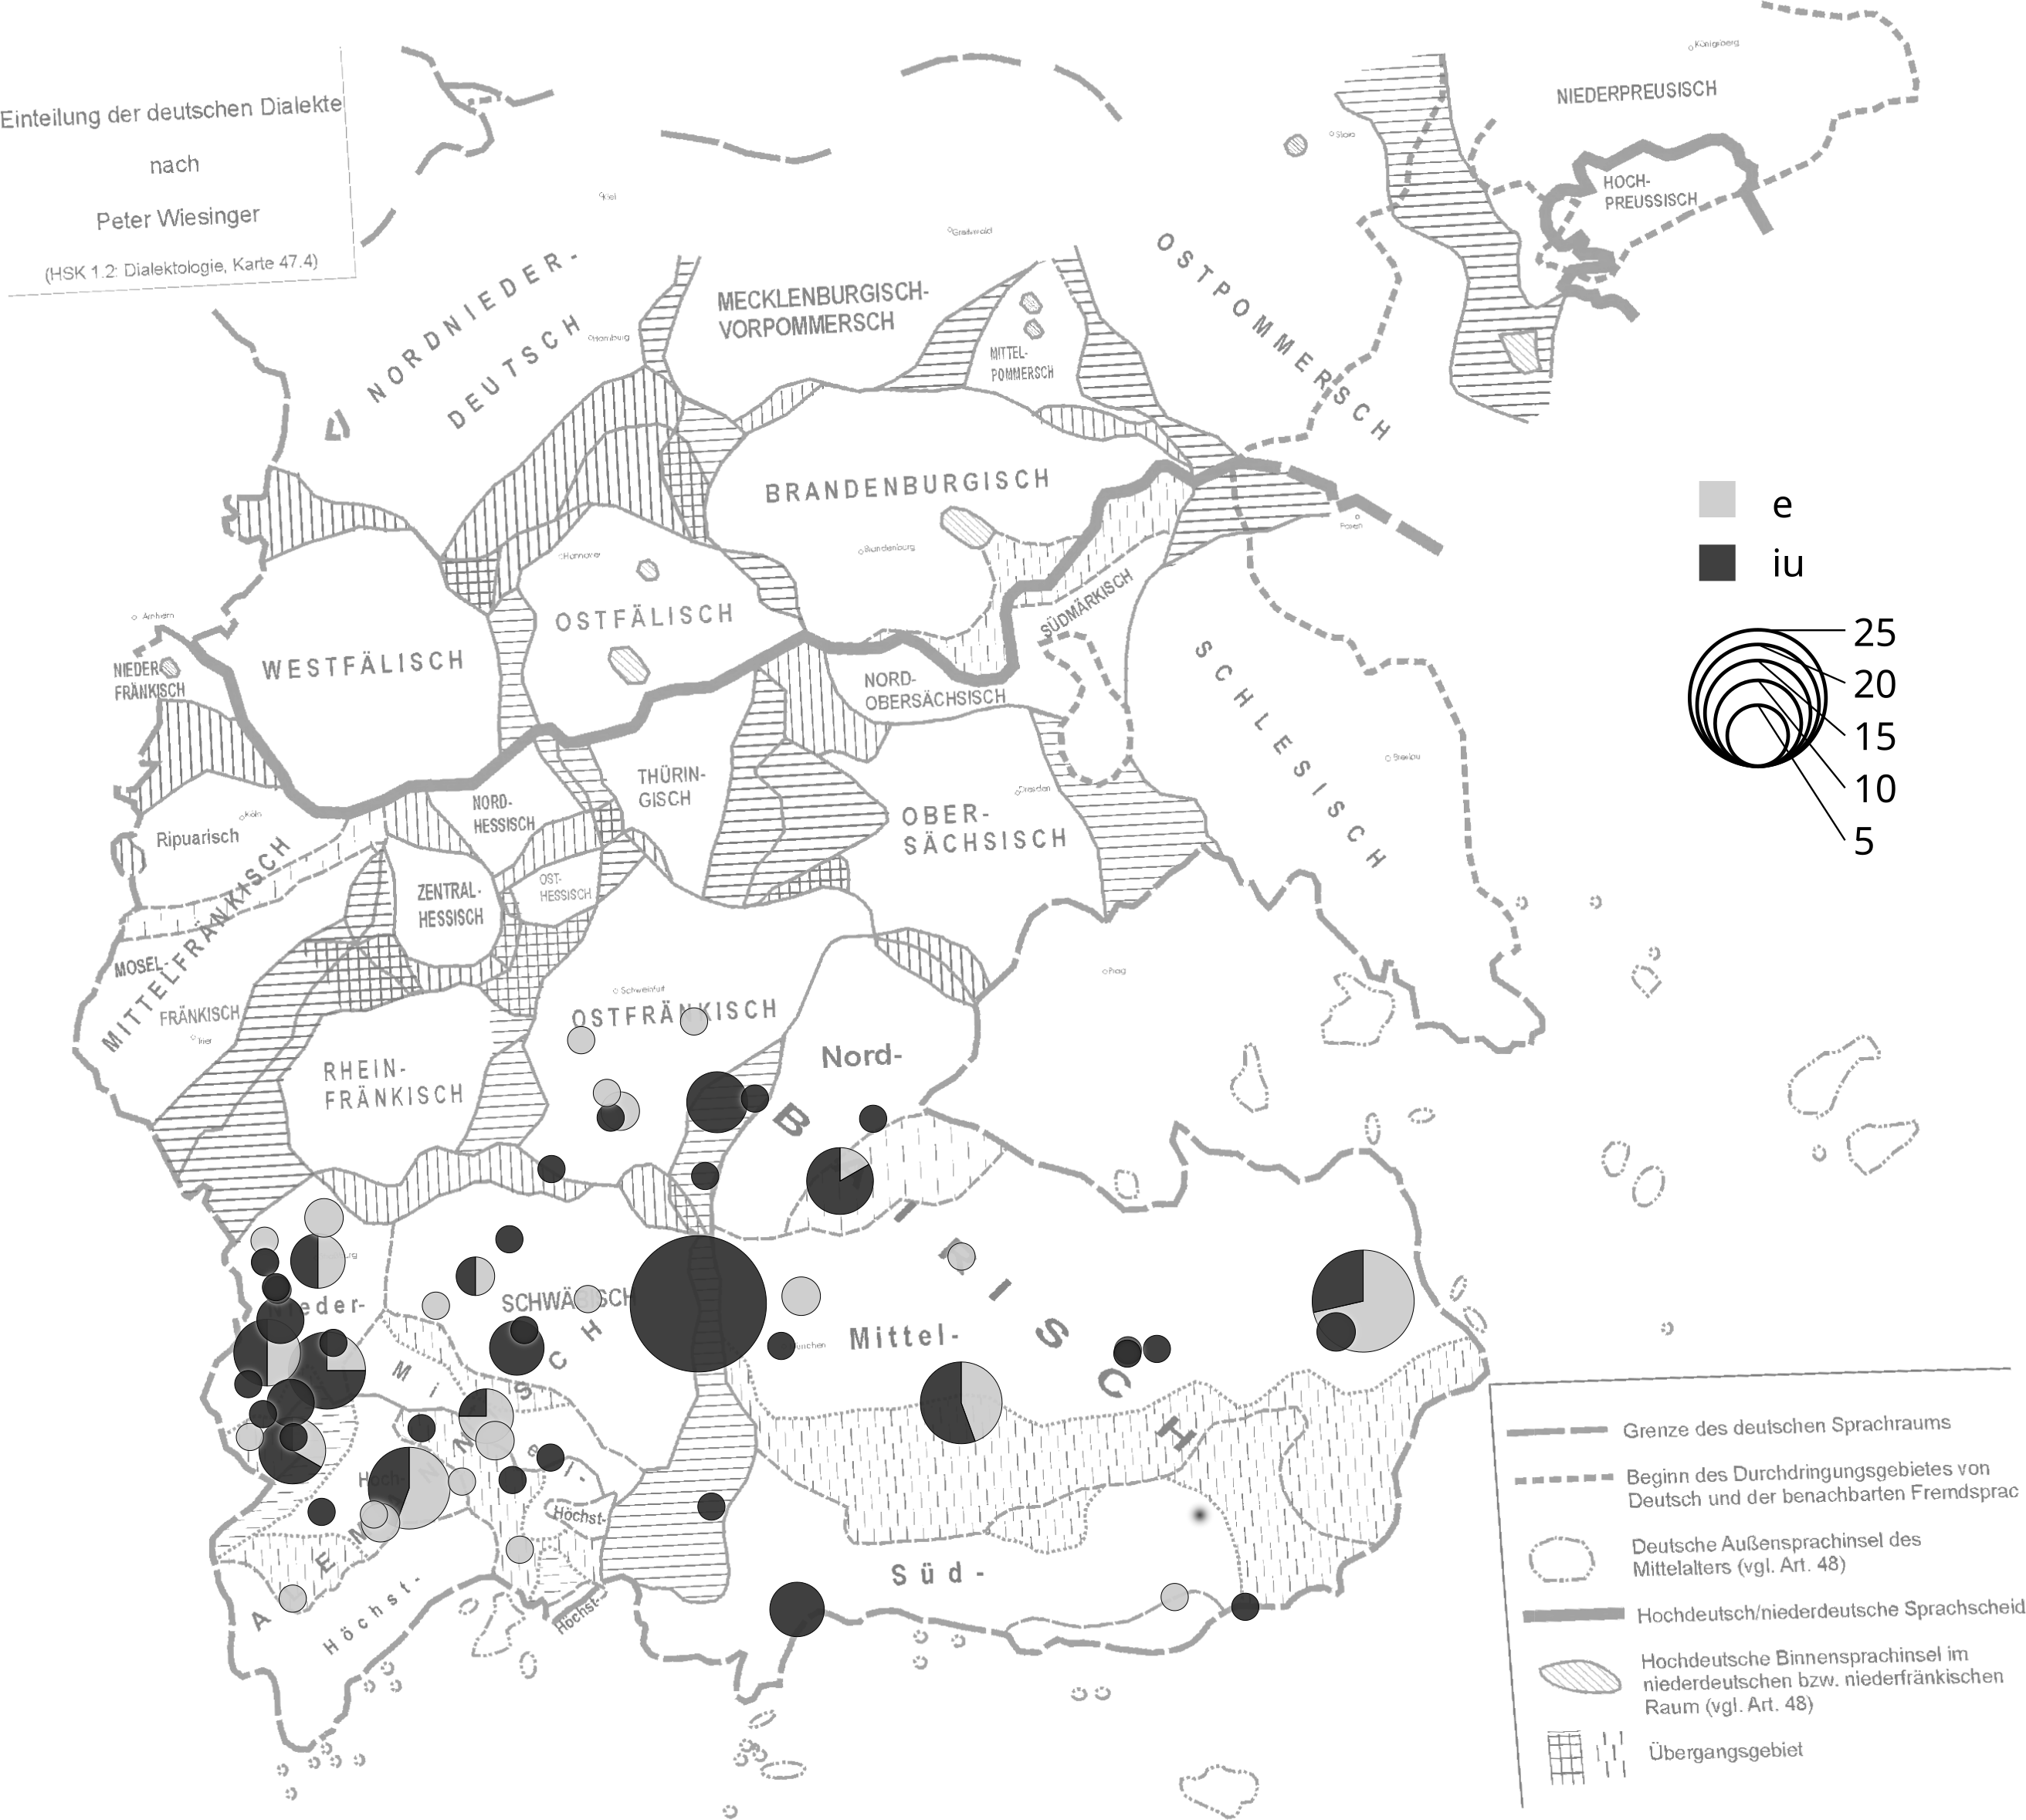
\includegraphics[
		width=.5\linewidth,
	]{./assets/grafiken/2021-07-12_cao_beide_iu-quant.png}
}
\subfloat[\norm{bėide} als Konjunktion (\norm{bėide} \textsc{x} \norm{unde} \textsc{y})]{
	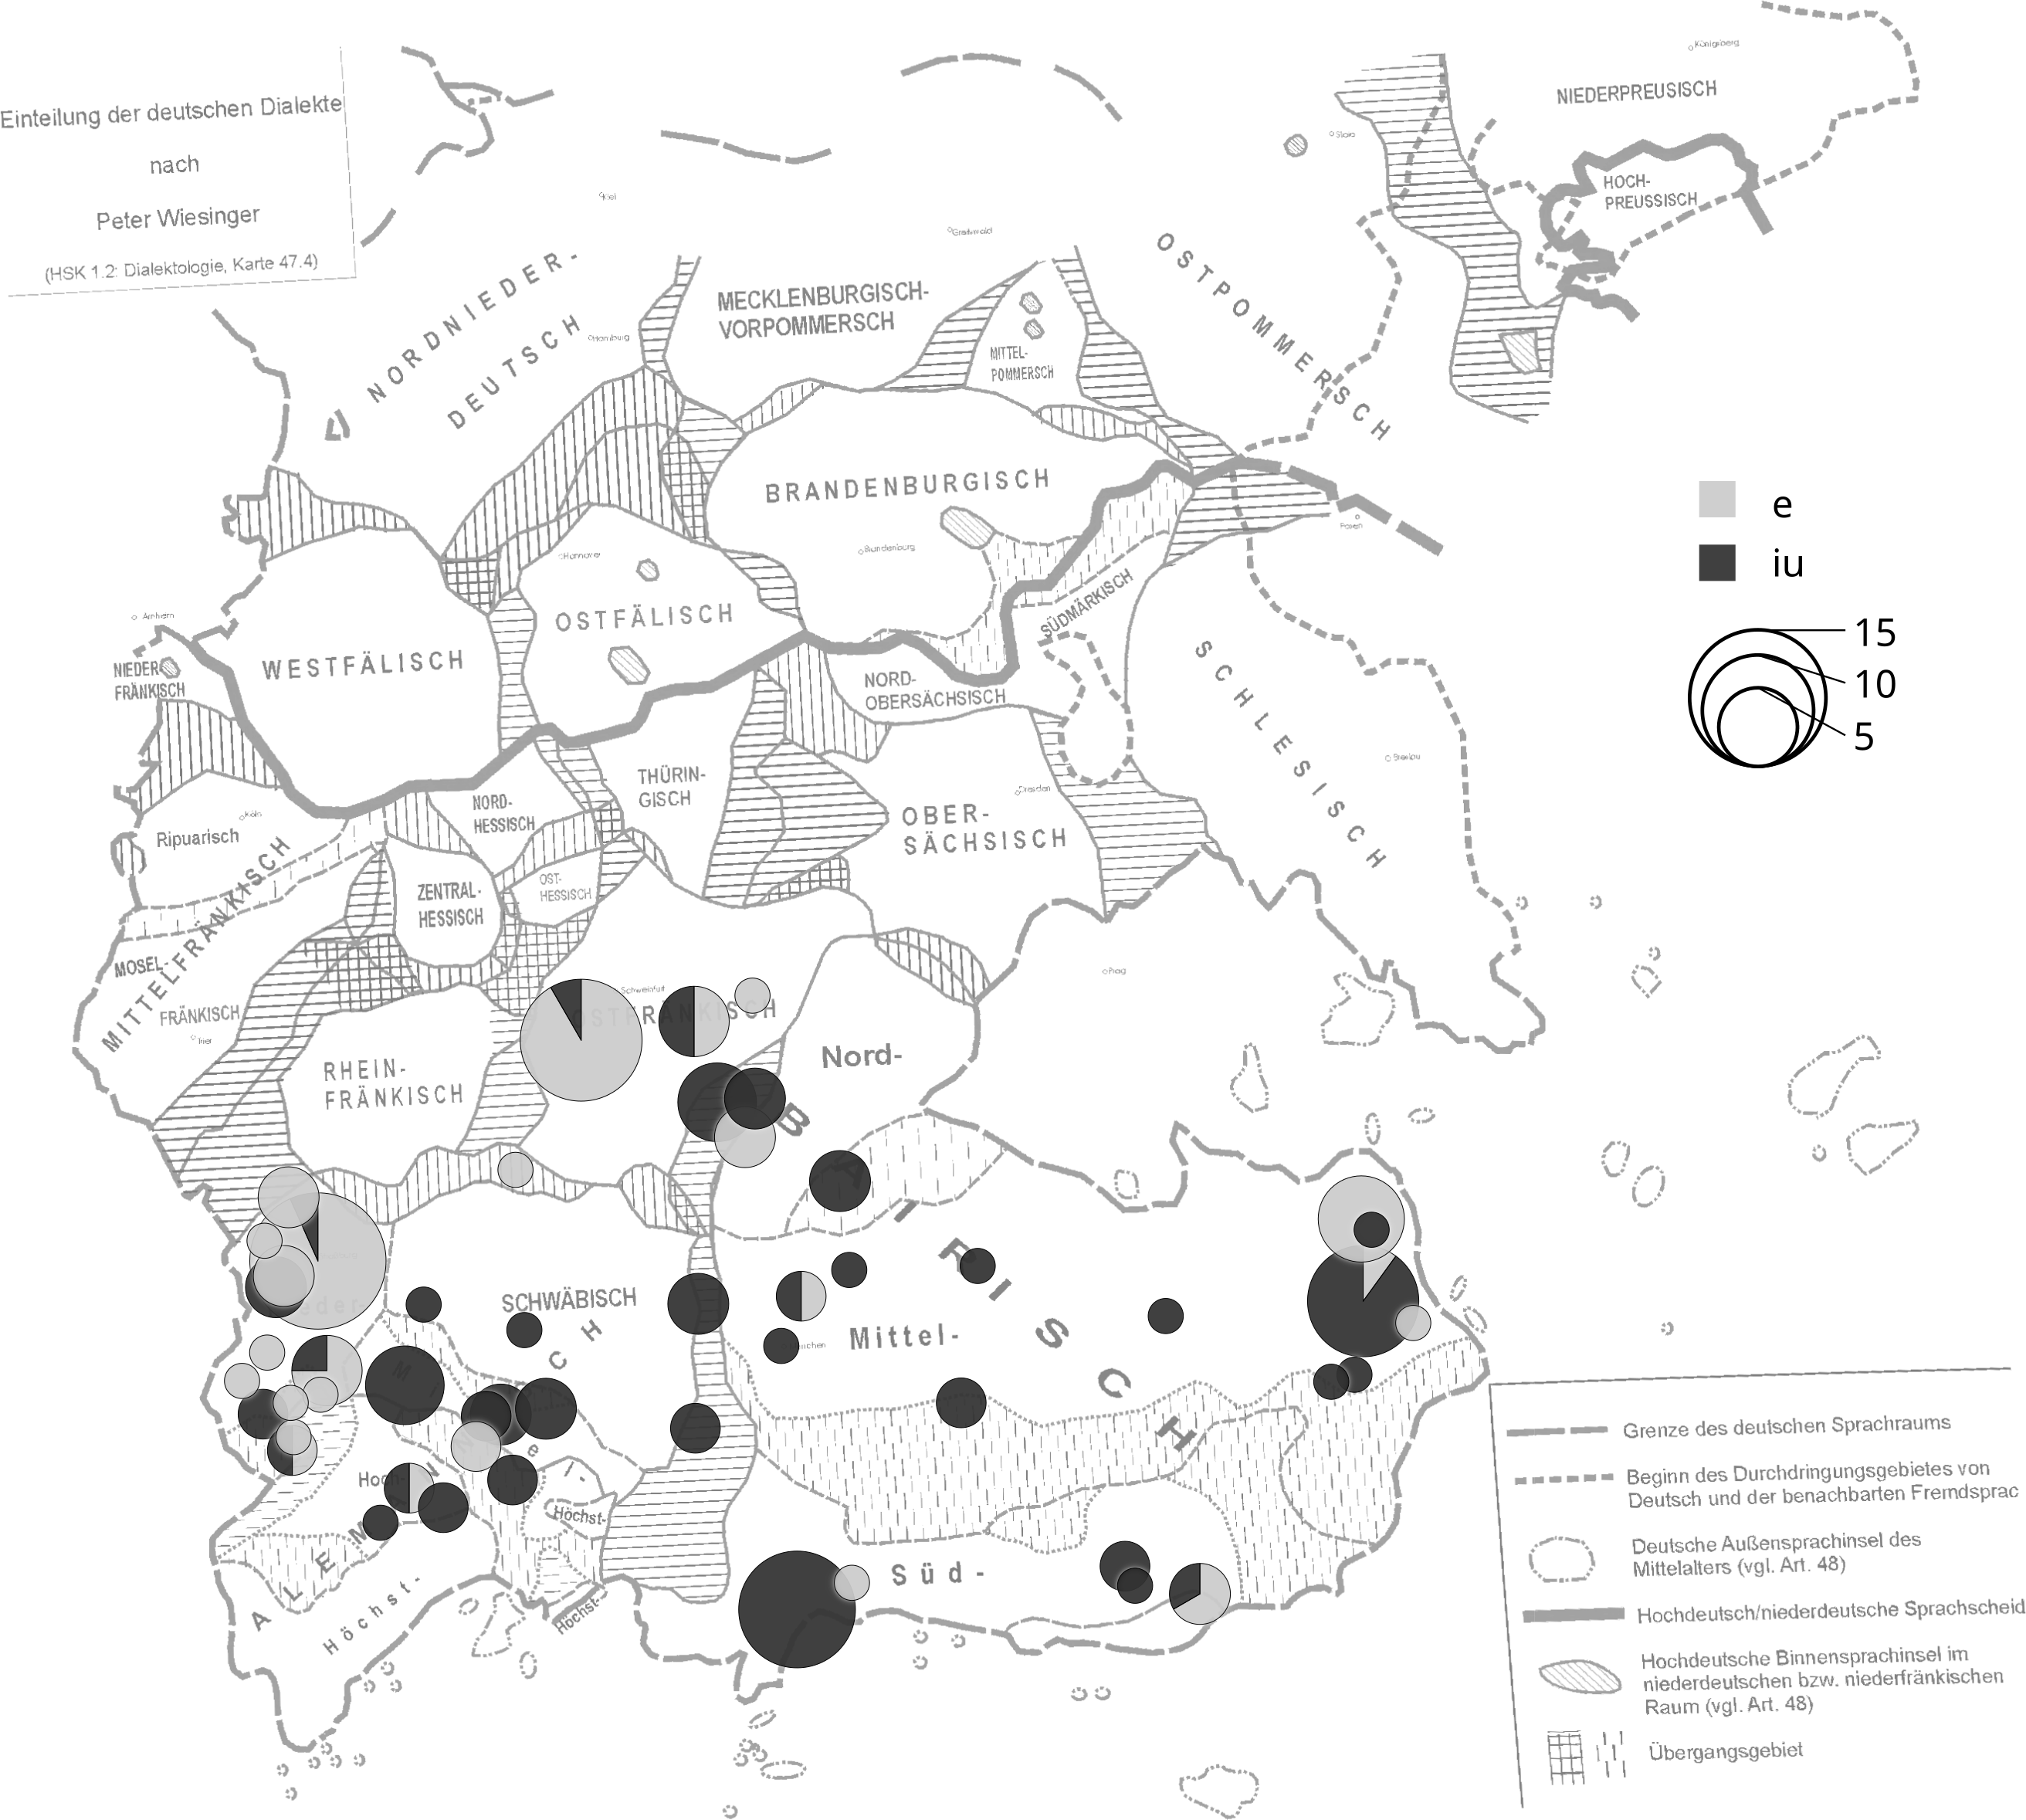
\includegraphics[
		width=.5\linewidth,
	]{./assets/grafiken/2021-07-12_cao_beide_iu-conj.png}
}
\caption{Die geografische Verteilung von \norm{e}- und \norm{iu}-Flexionstypen}
\label{fig:cao_beide_geofunctypes}
\end{figure}
\end{landscape}
}

Darüber hinaus liegt in je einem Fall Variation zwischen einer Urkunde und
ihrer Kopie bei ansonsten gleichem Wortlaut \cref{ex:intraurkvar1} sowie
Variation innerhalb derselben Urkunde vor \cref{ex:intraurkvar2}. Beide
Urkunden stammen aus dem ostfränkischen Sprachraum und illustrieren das dortige
Neben\-einander beider Formen.

\begin{exe}
\ex \label{ex:intraurkvar1}
	\begin{xlist}
	\ex \label{ex:intraurkvar1_1}
		\let\eachwordthree\eachwordtwo
		\let\eachwordtwo\eachwordone
		\glll vnd daz wir deſte baz \textbf{beide} der ſtat zu Wirceburg vnd
				deme lande den Vride gevurdern mugen \\
			Vnd daz wir deſte baz \textbf{beidu} der ſtat zu Wirceburg/ Vnd
				dem lande den fride gevurdern mugen \\
			und dass wir desto besser beide der Stadt zu Würzburg und dem Land 
				den Frieden fördern können \\
		\begin{taggedline}{\parencites(Würzburg, 1289)[\pno~1126~AB, 414.36--38 bzw.~37--39]{cao2}}
		\trans \wdef{damit wir den Frieden sowohl in der Stadt Würzburg als
			auch im Land umso besser fördern können}
		\end{taggedline}
	\end{xlist}

\ex \label{ex:intraurkvar2}
	\begin{xlist}
	\ex \label{ex:intraurkvar2_1}
		\gll aller anſprache / immerewiclichen gelazen \textbf{beidiv} Ledic
				vnde vri \\
			aller Anklage {} immer.ewiglich gelassen beide ledig und frei \\
		\begin{taggedline}{\parencites(Bamberg, 1295)[\pno~2293, 420.23]{cao3}}
		\trans \wdef{für immer und ewig aller Anklage sowohl ledig als auch frei
			gelassen}
		\end{taggedline}

	\ex \label{ex:intraurkvar2_2}
		\gll vnſer zinsgelt \textbf{beide} klein vnde groz \\
			unser Zinsgeld beide klein und groß \\
		\begin{taggedline}{\pnotecite[\pno~2293, 420.30]{cao3}}
		\trans \wdef{unser Zinsgeld, sowohl kleines als auch großes}
		\end{taggedline}
	\end{xlist}
\end{exe}

\subsection{Mit zwei Controllern}
\label{subsec:caokonj2ctrl}

Mit 59 Belegen ist die Koordination von zwei nominalen Elementen der häufigste
Anwendungsfall der Konstruktion \norm{bėide \dots\ unde} \wdef{sowohl \dots\
als auch} im untersuchten Material. Ein Beispiel für die hier diskutierten
Verwendungsweisen wird in \cref{ex:caokonj2ctrl} gegeben. Als Elemente, die
koordiniert werden, dienen einzelne Substantive \cref{ex:caokonj2ctrl_1},
Pronomina und Namen \cref{ex:caokonj2ctrl_2}, komplexe Nominalphasen
\cref{ex:caokonj2ctrl_3} oder auch freie Relativsätze \cref{ex:caokonj2ctrl_4}.
Gemeinsam ist den hier untersuchten Konjunkten, dass sie Controller enthalten.

\begin{exe}
\ex \label{ex:caokonj2ctrl}
	\begin{xlist}
	\ex \label{ex:caokonj2ctrl_1}
		\gll \textbf{beid\sscr{v}{ı}} reben vn̄ garten \\
			beide Reben und Garten \\
		\begin{taggedline}{\parencites(Basel, 1296)[\pno~2353, 462.28--29]{cao3}}
		\trans \wdef{sowohl Reben als auch Garten}
		\end{taggedline}

	\ex \label{ex:caokonj2ctrl_2}
		\gll \textbf{beidiv} ich / Vnd hainrich von meringen \\
			beide ich {} und Heinrich von Meringen \\
		\begin{taggedline}{\parencites(Kl.~Steingaden, Kr.~Weilheim-Schongau, 1291)[\pno~1347, 578.25]{cao1}}
		\trans \wdef{sowohl ich als auch Heinrich von Meringen}
		\end{taggedline}

	\ex \label{ex:caokonj2ctrl_3}
		\gll \textbf{beidv} er / vn̄ oͮch alle die / den er ſvͥ gît \\
			beide er {} und auch alle die {} denen er sie gibt \\
		\begin{taggedline}{\parencites(Hüfingen, Schwarzwald-Baar-Kr., 1292)[\pno~1566, 717.18]{cao2}}
		\trans \wdef{sowohl er als auch alle die, denen er sie gibt}
		\end{taggedline}

	\ex \label{ex:caokonj2ctrl_4}
		\gll \textbf{bediv} di nv lebent · vn̄ hernahe chvmftige ſint \\
			beide die nun leben {} und hernach künftig sind \\
		\begin{taggedline}{\parencites(Wien, 1291)[\pno~1352, 580.8]{cao2}}
		\trans \wdef{sowohl die nun leben als auch hernach künftig sind}
		\end{taggedline}
	\end{xlist}
\end{exe}

\cref{tab:caokoordnomctrl} listet die Belegzahlen für \norm{bėide} und
\norm{bėidiu} in Abhängigkeit der Personenmerkmale der Konjunkte auf. Es ist
zwar mit \citet[626]{ksw2} davon auszugehen, dass die koordinierten Elemente
ursprünglich appositiv zu einem pronominal gebrauchten \wdef{beide} waren
(\norm{bėide}, \textsc{x} \norm{unde} \textsc{y}). Aus der Belegverteilung im
Urkundenmaterial ist jedoch nicht \fw{per se} zu schließen, dass konjunktional
gebrauchtes \norm{bėide} bei der Koordination von nominalen Elementen noch
regelmäßig kongruiert.

\begin{table}[tp]
\centering
\caption{Form nach Personenmerkmalen nominaler Konjunkte}
\begin{tabular}{l l r r r}
\toprule
\textbf{Konjunkt 1}
	& \textbf{Konjunkt 2}
	& \textbf{bėid(e)}
	& \textbf{bėidiu}
	& \textbf{Summe}
	\\
\midrule

% Gleiches Geschlecht
\Fsg\subM         & \Fpl\subM         &    &  1 &  1 \\
\Fsg\subM         & \Tsg.\MascM       &  3 &  1 &  4 \\
\Tsg.\MascM       & \Tsg.\MascM       &  3 &  3 &  6 \\
\Tsg.\MascM       & \Tpl.\MascM       &    &  1 &  1 \\
\Tsg.\FemF        & \Tsg.\FemF        &    &  1 &  1 \\
%                                        6    7   13

\midrule

% Unterschiedliches Geschlecht
\Fsg\subM         & \Tsg.\FemF        &    &  1 &  1 \\
\Fsg\subF         & \Tsg.\MascM       &  1 &    &  1 \\
\Tsg.\MascM       & \Tsg.\FemF        &    &  1 &  1 \\
\Tpl.\FemF        & \Tpl.\MascM       &    &  2 &  2 \\
%                                        1    4    5

\midrule

% Mit gleichem Genus und egalem Geschlecht
\Fsg\subM         & \Tpl.\MascA       &  3 &    &  3 \\
\Tsg.\MascA       & \Tsg.\MascA       &  1 &  1 &  2 \\
\Tsg.\MascA       & \Tpl.\MascA       &    &  1 &  1 \\
\Tsg.\MascM       & \Tpl.\MascA       &    &  1 &  1 \\
\Tpl.\MascA       & \Tpl.\MascA       &  9 &  5 & 14 \\
\Tpl.\MascM       & \Tpl.\MascA       &  1 &    &  1 \\
\Tsg.\MascM       & \Tpl.\NeutA       &  1 &    &  1 \\
%                                       15    8   23

\midrule

% Mit unterschiedlichem Genus und egalem Geschlecht oder unbelebt
\Tsg.\NeutA       & \Tpl.\MascA       &    &  1 &  1 \\
\Tsg.\MascM       & \Tsg.\NeutI       &    &  1 &  1 \\
\Tpl.\MascA       & \Tpl.\NeutI       &  1 &  5 &  6 \\
%                                        1    7    8

\midrule

% Gleiches Genus (unbelebt)
\Tsg.\FemI        & \Tsg.\FemI        &    &  1 &  1 \\
\Tsg.\NeutI       & \Tsg.\NeutI       &  1 &    &  1 \\
\Tsg.\MascI       & \Tpl.\MascI       &  1 &    &  1 \\
%                                        2    1    3

\midrule

% Unterschiedliches Genus (unbelebt)
\Tsg.\MascI       & \Tsg.\NeutI       &    &  1 &  1 \\
\Tsg.\FemI        & \Tsg.\NeutI       &  1 &  1 &  2 \\
\Tsg.\NeutI       & \Tsg.\FemI        &    &  3 &  3 \\
\Tpl.\MascI       & \Tpl.\FemI        &  2 &    &  2 \\
\Tpl.\MascI       & \Tsg.\NeutI       &  1 &    &  1 \\
\Tpl.\FemI        & \Tsg.\MascI       &    &  1 &  1 \\
\Tpl.\FemI        & \Tpl.\MascI       &    &  1 &  1 \\
%                                        4    7   11

\midrule
\mc{2}{l}{Summe}                      & 29 & 34 & 63 \\
\bottomrule
\end{tabular}
\label{tab:caokoordnomctrl}
\end{table}

Der erste Abschnitt in \cref{tab:caokoordnomctrl} enthält Konjunkte mit
gleichwertigen Genus- und Sexus\-merkmalen ($\MascM+\MascM{}$ und
$\FemF+\FemF$). Anders als bisher beobachtet, steht in 54\pct\ der Fälle die
ansonsten neutrale Form \norm{bėidiu}. Im dritten Abschnitt, der mindestens ein
Element mit irrlevantem Sexus enthält, das formal jedoch maskulin ist (\MascA,
zum Beispiel
% \norm{liute}
\norm{lǖte} \wdef{Leute},
% \norm{burgære}
\norm{burgǟre} \wdef{Bürger}), und einem weiteren solchen oder einem
maskulin-männlichen Element ($\MascA+\MascA{}$ und $\MascM+\MascA$)
häufen sich dagegen die Belege bei \norm{bėid(e)}, das 65\pct\ der für diesen
Kontext belegten Formen ausmacht. Im letzten Abschnitt der Tabelle, der
unbelebte Elemente mit unterschiedlichem Genus enthält, wird anders als zuvor
\norm{bėidiu} nicht klar favorisiert: Mit 58\pct\ für \norm{bėidiu} sind die
Verhältnisse nahezu ausgeglichen. Insgesamt ergibt sich keine klare, von
Personenmerkmalen abhängige Verteilung.

Für den zweiten Abschnitt mit unterschiedlichen Geschlechtsmerkmalen belebter
Konjunkte scheint eine klare Präferenz für \norm{bėidiu} vorzuliegen, die
ähnlich eindeutig zu sein scheint wie bei der Verwendung von \norm{bėide} als
Quantor. Dasselbe gilt für die vierte Gruppe mit Kombinationen mit
unspezifischem Geschlecht sowie belebten mit unbelebten Konjunkten enthalten.
Sollte dies als Evidenz für Gender Resolution dienen? \citet[187]{gjelsten1980}
räumt in ihrer Kritik an \posscite{askedal1974} Arbeit zu konjunktionalem
\norm{bėide} ein, dass bei substantivischen Konjunkten nicht klar zwischen
pronominalem Gebrauch (\norm{bėide}, \textsc{x} \norm{unde}~\textsc{y}) und
konjunktionalem (\norm{bėide}~\textsc{x} \norm{unde}~\textsc{y}) unterschieden
werden kann. Angesichts der recht homogenen Verteilung der Formen \norm{bėide}
und \norm{bėidiu} ist aber nicht davon auszugehen, dass ausgerechnet hier
plötzlich regelmäßig Kongruenz zwischen \norm{bėide} und den Konjunkten
herrscht.

\cref{tab:caokoordnomctrl} trennt nicht nach Kasus; die folgende
\cref{tab:caokoordnomctrlcase} stellt die Verteilung zumindest der
Kombinationen von Konjunkten dar, die eine klare Zuordnung des Geschlechts
erlaubt. Belege mit Gruppenbezeichnungen wie \norm{lǖte} \wdef{Leute
(\MascA)}, \norm{arme} \wdef{Arme (\MascA)} und \norm{alle die, den ęr si
gibet} \wdef{alle die (\MascA?), denen er sie gibt} sowie Kombinationen von
belebten und unbelebten Konjunkten wie in \norm{lǖte unde guet} \wdef{Leute
(\MascA) und Gut (\NeutI)} wurden nicht gewertet. Bei allen diesen Belegen ist
ohnehin nur \norm{bėide} für den Nom., Akk.\ und den Dat.\ belegt; für den
Gen.\ liegen keine Belege vor.

\begin{table}
\centering
\caption{Form nach dem Kasus nominaler Konjunkte}
\begin{tabularx}{\linewidth}{
	l
	R R c R R
	c
	R R c R R
	r
}
\toprule
\mr{3}{*}[-1ex]{\textbf{Kasus}}
	& \mc{5}{c}{belebt}
	& % --
	& \mc{5}{c}{unbelebt}
	& \mr{3}{*}[-1ex]{\textbf{Summe}}
	\\

\cmidrule{2-6}
\cmidrule{8-12}

%
	& \mc{2}{c}{gleich}
	& % --
	& \mc{2}{c}{verschieden}
	& % --
	& \mc{2}{c}{gleich}
	& % --
	& \mc{2}{c}{verschieden}
	& % --
	\\

\cmidrule{2-3}
\cmidrule{5-6}
\cmidrule{8-9}
\cmidrule{11-12}

%
	& \textbf{bėid(e)}
	& \textbf{bėidiu}
	& % --
	& \textbf{bėid(e)}
	& \textbf{bėidiu}
	& % --
	& \textbf{bėid(e)}
	& \textbf{bėidiu}
	& % --
	& \textbf{bėid(e)}
	& \textbf{bėidiu}
	& % --
	\\

\midrule

\Nom
	& 4
	& 4
	& % --
	& 1
	& 2
	& % --
	& %
	& %
	& % --
	& %
	& 3
	& 14
	\\

\midrule

\Acc
	& 2
	& %
	& % --
	& %
	& %
	& % --
	& 3
	& %
	& % --
	& 2
	& 3
	& 10
	\\

\midrule

\Dat
	& %
	& 2
	& % --
	& %
	& 1
	& % --
	& %
	& %
	& % --
	& 1
	& 1
	& 5
	\\

\midrule

\Gen
	& %
	& 1
	& % --
	& %
	& 1
	& % --
	& %
	& %
	& % --
	& 1
	& %
	& 3
	\\

\midrule

Summe
	& 6
	& 7
	& % --
	& 1
	& 4
	& % --
	& 3
	& %
	& % --
	& 4
	& 7
	& 32
	\\

\bottomrule
\end{tabularx}
\label{tab:caokoordnomctrlcase}
\end{table}

Bei der Betrachtung nach Kasus ergibt sich für den Nom./Akk.\ keine klare
Präferenz bei belebten Konjunkten mit gleichem Geschlecht, da hier die
Verhältnisse nahezu ausgeglichen sind. Für Kombinationen mit verschiedenem
belebten Geschlecht liegen zu wenige Belege vor, um eine Regel aufzustellen.
Dasselbe gilt für die drei Belege für \norm{bėide} bei gleichem unbelebten
Genus. Bei verschiedenem unbelebten Genus entfällt der Großteil der Belege auf
\norm{bėidiu}.

Darüber hinaus liegen allerdings auch Belege für \norm{bėide} und \norm{bėidiu}
im Dativ und Genitiv vor. Wenn \norm{bėide} entsprechend der formalen
Merkmale der jeweiligen NP flektieren würde, dürften diese Formen nicht
auftreten. Nun ist nicht auszuschließen, dass die Flexionskategorie Kasus in
diesem Fall wegfällt, das Geschlecht beziehungsweise Genus der Konjunkte aber
trotzdem eine Auswirkung auf die Form der Konjunktion hat. Abgesehen von je
einem Beleg für \norm{bėide} bei verschiedenem unbelebten Genus steht in den
vereinzelten belegten Fällen \norm{bėidiu}.

Insgesamt ist keine deutliche Häufung auf \norm{bėide} bei gleichem belebtem
Geschlecht sowie auf \norm{bėidiu} bei unbelebtem Bezug unabhängig vom Genus
auszumachen, wie dies bei der quantifizierenden Verwendung der Fall war.
Angesichts der vereinzelten Belege in den einzelnen Kasusfeldern kann wohl auch
für belebte Konjunkte mit verschiedenem Geschlecht keine Regel für das
Auftreten von \norm{bėidiu} abgeleitet werden. Wenn sich Belege mit
pronominalem \norm{bėide} eingeschlichen haben sollten, treten diese nicht klar
aus der Statistik hervor.

\subsection{Mit zwei Targets}
\label{subsec:caobeidkoordtarg}

Parallel zur Auswertung in \cref{subsubsec:beid2p2coordncao} zum Einfluss der
Personenmerkmale auf die Form von \norm{bėide} beim indirekten Bezug auf
kombinierte nominale Controller lassen sich auch für die Konjunktion
\norm{bėide} solche Konjunkte untersuchen, die selbst keine Personenmerkmale
definieren, sondern Kongruenz\-targets darstellen. In der Stichprobe sind dies
konkret verschiedene Arten von Adjektiven, die in \cref{ex:caobeidkoordtarg}
beispielhaft angeführt sind: vorangestellt attributive
\cref{ex:caobeidkoordtarg_1}, nachgestellt attributive
\cref{ex:caobeidkoordtarg_2} und prädikative \cref{ex:caobeidkoordtarg_3},
wobei die Zuordung bei Nachstellung nicht immer eindeutig ist.

\begin{exe}
\ex \label{ex:caobeidkoordtarg}
	\begin{xlist}
	\ex \label{ex:caobeidkoordtarg_1}
		\gll \textbf{beide} geiſtliches / vn̄ wertliches gerihtes \\
			beide geistlich-\Gen.\Sg.\NeutI.\St{} {} und
			weltlich-\Gen.\Sg.\NeutI.\St{} Gericht-\Gen.\Sg{}[\NeutI] \\
		\begin{taggedline}{\parencites(Bamberg, 1293)[\pno~1764, 71.26]{cao3}}
		\trans \wdef{sowohl geistlichen als auch weltlichen Gerichts}
		\end{taggedline}

	\ex \label{ex:caobeidkoordtarg_2}
		\gll erberge leut \textbf{peideu} gaiſtlich vnd wertlich \\
			ehrenhafte Leute[\Nom.\Pl.\MascA] beide geistlich[\Nom.\Pl.\MascA]
			und weltlich[\Nom.\Pl.\MascA] \\
		\begin{taggedline}{\parencites(Engelthal, Kr.~Nürnberger Land, 1289)[\pno~1153, 431.44]{cao2}}
		\trans \wdef{sowohl geistliche und weltliche ehrenhafte Leute}
		\end{taggedline}

	\ex \label{ex:caobeidkoordtarg_3}
		\gll vnde hat {div ſelben} gvͦt \textelp{} aller anſprache /
			immerewiclichen gelazen \textbf{beidiv} Ledic vnde vri \\
			und hat dieselben Gut[\Acc.\Pl.\NeutI] {} aller Anklage {}
			immer.und.ewig gelassen beide ledig[\Acc.\Pl.\NeutI] und
			frei[\Acc.\Pl.\NeutI] \\
		\begin{taggedline}{\parencites(Bamberg, 1295)[\pno~2293, 420.21--23]{cao3}}
		\trans \wdef{und hat dieselben Güter \textelp{} immer und ewig sowohl
			ledig als auch frei von aller Anklage gelassen}
		\end{taggedline}
	\end{xlist}
\end{exe}

Auch für die Koordination von Adjektiven lässt sich keine regelmäßige
Korrespondenz zwischen der Kombination bestimmter Personenmerkmale und
konjunktional gebrauchtem \norm{bėide} feststellen, wie
\cref{tab:caokoordtarg} zeigt. Für Konjunkte mit gleichen Genus- und
Sexusmerkmalen liegt nur ein einziger Beleg vor; bei der Konjunktion von
maskulinen Targets mit beliebigem Sexus sind die Verhältnisse nahezu
ausgeglichen, insofern in 57\pct\ der Fälle \norm{bėide} belegt ist. Bei den
unbelebten Targets mit unterschiedlichem Genus steht in 64\pct\ der Belege
\norm{bėidiu}.

\begin{table}
\centering
\caption{Form nach Personenmerkmalen adjektivischer Konjunkte}
\begin{tabular}{l l r r r}
\toprule
\textbf{Konjunkt 1}
	& \textbf{Konjunkt 2}
	& \textbf{bėid(e)}
	& \textbf{bėidiu}
	& \textbf{Summe}
	\\
\midrule

% Gleiches Geschlecht
\FemF.\Sg        & \FemF.\Sg  &  1 &    &  1 \\

\midrule

% Mit gleichem Genus und egalem Geschlecht
\MascA.\Pl       & \MascA.\Pl &  4 &  3 &  7 \\

\midrule

% Gleiches Genus (unbelebt)
\MascI.\Sg       & \MascI.\Sg &  1 &  3 &  4 \\
\FemI.\Sg        & \FemI.\Sg  &    &  1 &  1 \\
\NeutI.\Sg       & \NeutI.\Sg &  4 &  1 &  5 \\
\NeutI.\Pl       & \NeutI.\Pl &    &  1 &  1 \\
%                                5    6   11

\midrule
\mc{2}{l}{Summe}              & 10 &  9 & 19 \\
\bottomrule
\end{tabular}
\label{tab:caokoordtarg}
\end{table}

% Blickt man auch hier auf die Verteilung der Belege nach Kasus, ergibt sich,
% dass von einer klaren Präferenz für \norm{bėidiu} bei unbelebtem Bezug wie
% bei der Verwendung als Quantor keine Rede sein kann. Auch in
% \cref{tab:caokoordtargcase} wurden Gruppenbezeichnungen wie \norm{lǖte}
% \wdef{Leute (\MascA)} ignoriert. Neben einem einzelnen \norm{bėide}-Beleg für
% die Kombination von zwei Konjunkten mit gleichem Geschlecht im Nominativ
% liegen lediglich Belege für gleiches unbelebtes Genus vor. Diese verteilen
% sich insgesamt gleichmäßig auf \norm{bėide} und \norm{bėidiu}, wobei
% zumindest im Akk.\ drei von vier Belegen auf \norm{bėidiu} entfallen.
% Umgekehrt liegen im Gen.\ drei von vier Belegen für \norm{bėide} vor, im
% Dat.\ zwei von drei für \norm{bėidiu}. Bei den hier nicht aufgeführten
% Belegen mit unbestimmtem Geschlecht entfallen im Nom.\ zwei auf \norm{bėide},
% drei auf \norm{bėidiu} und im Dat.\ zwei auf \norm{bėide}. Für den Akk.\ und
% den Gen.\ liegen keine Belege vor.

% \begin{table}
% \centering
% \caption{Verteilung der \wdef{beide}-Formen in Abhängigkeit des Kasus
% adjektivischer Konjunkte}
% \begin{tabularx}{.75\linewidth}{
% 	l
% 	R R % c R R
% 	c
% 	R R % c R R
% 	r
% }
% \toprule
% \mr{3}{*}[-.5ex]{\textbf{Kasus}}
% 	& \mc{2}{c}{belebt} % \mc{5}{c}{belebt}
% 	& % --
% 	& \mc{2}{c}{unbelebt} % \mc{5}{c}{unbelebt}
% 	& \mr{3}{*}[-.5ex]{\textbf{Summe}}
% 	\\

% % \cmidrule{2-3} % \cmidrule{2-6}
% % \cmidrule{5-6} % \cmidrule{8-12}

% % %
% % 	& \mc{2}{c}{gleich}
% % 	% & % --
% % 	% & \mc{2}{c}{verschieden}
% % 	& % --
% % 	& \mc{2}{c}{gleich}
% % 	% & % --
% % 	% & \mc{2}{c}{verschieden}
% % 	& % --
% % 	\\

% \cmidrule{2-3}
% \cmidrule{5-6}
% % \cmidrule{8-9}
% % \cmidrule{11-12}

% %
% 	& \textbf{bėid(e)}
% 	& \textbf{bėidiu}
% 	% & % --
% 	% & \textbf{bėid(e)}
% 	% & \textbf{bėidiu}
% 	& % --
% 	& \textbf{bėid(e)}
% 	& \textbf{bėidiu}
% 	% & % --
% 	% & \textbf{bėid(e)}
% 	% & \textbf{bėidiu}
% 	& % --
% 	\\

% \midrule

% \Nom
% 	& 1
% 	& %
% 	% & % --
% 	% & %
% 	% & %
% 	& % --
% 	& 1
% 	& %
% 	% & % --
% 	% & %
% 	% & %
% 	& 2
% 	\\

% \midrule

% \Acc
% 	& %
% 	& %
% 	& % --
% 	% & %
% 	% & %
% 	% & % --
% 	& 1
% 	& 3
% 	% & % --
% 	% & %
% 	% & %
% 	& 4
% 	\\

% \midrule

% \Dat
% 	& %
% 	& %
% 	% & % --
% 	% & %
% 	% & %
% 	& % --
% 	& 1
% 	& 2
% 	% & % --
% 	% & %
% 	% & %
% 	& 3
% 	\\

% \midrule

% \Gen
% 	& %
% 	& %
% 	% & % --
% 	% & %
% 	% & %
% 	& % --
% 	& 3
% 	& 1
% 	% & % --
% 	% & %
% 	% & %
% 	& 4
% 	\\

% \midrule

% Summe
% 	& 1
% 	& %
% 	% & % --
% 	% & %
% 	% & %
% 	& % --
% 	& 6
% 	& 6
% 	% & % --
% 	% & %
% 	% & %
% 	& 13
% 	\\

% \bottomrule
% \end{tabularx}
% \label{tab:caokoordtargcase}
% \end{table}

\subsection{Rein syntaktischer Kontext}
\label{subsec:caobeidquantsyncont}

Im Urkundenmaterial kommt neben der Konjunktion von Controllern und Targets,
die Personenmerkmale definieren beziehungsweise widerspiegeln, auch die
Konjunktion solcher Elemente vor, die keinerlei Personenmerkmale definieren.
Die Konstruktion \norm{bėide \dots\ unde} \wdef{sowohl \dots\ als auch} hat
hier insofern funktionalen Charakter, als \norm{bėide} als Fokuspartikel dient,
die die Zweiheit der Optionen betont \autocites(siehe auch
\cref{sec:ovwbeideconj})[425--428]{johannessen2005}.
% 
% \begin{exe}
% \ex \label{ex:beidenoagr}
% 	\begin{xlist}
% 	\ex[]{(allen) beiden$_{i+j}$, Sabine$_i$ und Peter$_j$}
% 		\label{ex:beidenoagr_1}
% 
% 	\ex[*]{(allen) beiden$_{i+j}$, hier$_i$ und in Berlin$_j$}
% 		\label{ex:beidenoagr_2}
% 	\end{xlist}
% \end{exe}
% 
Im exzerpierten Material kommt \norm{bėide} in diesem Zusammenhang mit
Temporaladverbien \cref{ex:caokoordsyn_1}, Lokaladverbien
\cref{ex:caokoordsyn_2} und Präpositionalphrasen
\crefrange{ex:caokoordsyn_2}{ex:caokoordsyn_3} vor.

\begin{exe}
\ex \label{ex:caokoordsyn}
	\begin{xlist}
	\ex \label{ex:caokoordsyn_1}
		\gll \textbf{beide} vor vn̄ noͤch \\
			beide vor und nach \\
		\begin{taggedline}{\parencites(Straßburg, 1295)[\pno~N~689, 499.25]{cao5}}
		\trans \wdef{sowohl davor als auch danach}
		\end{taggedline}

	\ex \label{ex:caokoordsyn_2}
		\gll \textbf{beide} da vn̄ an allin ſteitin \\
			beide da und an allen Stätten \\
		\begin{taggedline}{\parencites(Rosheim, Dépt.~Bas-Rhin, 1286)[\pno~N~321, 245.24]{cao5}}
		\trans \wdef{sowohl dort als auch an allen \textins{anderen} Orten}
		\end{taggedline}

	\ex \label{ex:caokoordsyn_3}
		\gll \textbf{baidev} zv Dorfe vnd ze velde \\
			beide zu Dorf-\Dat.\Sg{} und zu Feld-\Dat.\Sg{} \\
		\begin{taggedline}{\parencites(Michelstetten, Bz.~Mistelbach, 1299)[\pno~3319, 461.28]{cao4}}
		\trans \wdef{sowohl im Dorf als auch auf dem Feld}
		\end{taggedline}
	\end{xlist}
\end{exe}

In \cref{tab:caokoordsyn} werden der Vollständigkeit halber die Belegzahlen pro
Kombination der Wortart oder des Phrasentyps der Konjunkte aufgelistet. Eine
auffällige Häufung, die Anlass dazu geben würde, eine Präferenz in Abhängigkeit
der Konjunkte anzunehmen, ist auch hier nicht gegeben. Mit Ausnahme von zwei
bairisch-österreichischen Belegen aus Fallbach (Bz.~Mistelbach) und eines aus
St.~Paul im Lavanttal (Bz.~Wolfsberg) stammen die Belege für die Form
\norm{bėide} sämtlich aus dem alemannischen Sprachraum. Die Belege für
\norm{bėidiu} stammen umgekehrt hauptsächlich aus dem bairischen Sprachraum.

\begin{table}
\centering
\caption{Form nach Wortart adverbialer und präpositionaler Konjunkte}
\begin{tabular}{l l r r r}
\toprule
\textbf{Konjunkt 1}
	& \textbf{Konjunkt 2}
	& \textbf{bėid(e)}
	& \textbf{bėidiu}
	& \textbf{Summe}
	\\
\midrule

Adv     & Adv     &  2 &  1 &  3 \\

\midrule

PP      & AdvP    &  2 &    &  2 \\
AdvP    & PP      &  1 &    &  1 \\
%                    3    0    3

\midrule

PP      & PP      & 10 & 27 & 37 \\

\midrule
\mc{2}{l}{Summe}  & 15 & 28 & 43 \\
\bottomrule
\end{tabular}
\label{tab:caokoordsyn}
\end{table}

\subsection{Zusammenfassung}

Die aus dem \citetitle{cao} exzerpierten Belege zu \norm{bėide} als Konjunktion
bestätigen die in \citet[626--627]{ksw2} formulierte Beobachtung, dass die Form
in diesem Kontext nicht mehr nach grammatischen Kriterien variiert, sondern
freie Variation zwischen \norm{bėide} und \norm{bėidiu} vorliegt. Weder mit
koordinierten Controllern noch mit koordinierten Targets wird eine eindeutige
Abhängigkeit der Form der Konjunktion von den Personenmerkmalen der Konjunkte
deutlich. Dass der Aspekt von \norm{bėide} als Fokuspartikel
\autocites(siehe auch \cref{sec:ovwbeideconj})[425--428]{johannessen2005} in
diesem Kontext vorherrscht, ist auch daran zu erkennen, dass \norm{bėide}
regelmäßig mit solchen Konjunkten auftritt, die keinerlei Personenmerkmale
definieren oder reflektieren, sodass kein Kontext vorliegt, in dem Kongruenz
angewendet werden kann.

Auch die geografische Verteilung betreffend decken sich die
\citetitle{cao}-Belege mit den Aussagen in \citet[627--628]{ksw2}. Belege für
den Typ \norm{bėide} verteilen sich vor allem auf das
\mbox{(Nieder-)}\allowbreak{}Alemannische und Ostfränkische, im bairischen und
schwäbischen Sprachraum steht dagegen hauptsächlich \norm{bėidiu}. Ein
Unterschied zwischen \norm{-e} und \norm{-iu} anhand der syntaktischen Funktion
von \norm{bėide} macht sich nur insofern bemerkbar, als die Form bei
konjunktionalem Gebrauch in den Belegen zu Straßburg, Konstanz, Salzburg und
Wien deutlich erstarrt erscheint, während beim Quantor zumindest an den drei
zuletzt genannten Orten beide Flexionsformen auftreten.

\chapter{Auswertung zur \tit{Kaiserchronik}}
\label{ch:kcanalyse}

Wie im Analysekapitel zum \tit{Corpus der altdeutschen Originalurkunden} (\CAO)
werden im Folgenden zunächst die gesammelten Belege dialektgeografisch
eingeordnet. Danach folgt die Untersuchung der Verteilung der Formen des
Quantors \norm{bėide} in Bezug auf die unterschiedlichen morphosyntaktischen
Kontexte, in denen er belegt ist. Zunächst sollen diejenigen Kontexte
beleuchtet werden, in denen \norm{bėide} von Substantiven sowie Pronomina
abhängt und deren Personenmerkmale durch Kongruenz reflektiert. In einem
zweiten Teil wird nach möglichen Effekten der Distanz zwischen Controller und
Target gefragt. Der dritte Abschnitt schließt dieses Kapitel mit einer
Untersuchung von \norm{bėide} als Konjunktion in Anlehnung an die
Untersuchungen von \citet{askedal1974} und \citet{gjelsten1980} ab. Wie zuvor
wird jeweils ein tabellarischer Überblick über die Belegverteilung gegeben.
Einzelfälle, Ausnahmen und Zweifelsfälle werden exemplarisch diskutiert. Da die
\tit{Kaiserchronik} (\KC{}) in einer Vielzahl von Handschriften überliefert
ist, werden dabei wenn möglich relevante Parallelbelege hinzugezogen.

\section{Verteilung der gesammelten Belege in Zeit und Raum}
\label{subsec:beiddispmap}

Die Karte in \cref{fig:kartebelegzahl} zeigt die Menge der pro Handschrift
exzerpierten Belege für mhd.\ \norm{bėide} pro Ort beziehungsweise Gebiet. Dabei
sticht besonders das bairische Sprachgebiet heraus. Dies ist dem Umstand
geschuldet, dass die \KC{} vor allem im bairisch-österreichischen Raum
überliefert ist \autocite{klein1988}. Dezidiert alemannische Textzeugen, die
sich unter geografischen Gesichtspunkten mehr oder weniger direkt mit dem
Großteil der Urkundenbelege vergleichen ließen, sind abgesehen von K
(mittelalemannisch) nur unter den Fragmenten zu finden, die bei der
vorliegenden Arbeit nicht berücksichtigt wurden.%
%
	\footnote{Die Liste der Handschriftensiglen befindet sich im
		Literaturverzeichnis und richtet sich nach \citetitle{kcdigital} unter
		\citeurl{kcdigital}.%
	}

\begin{figure}
\centering
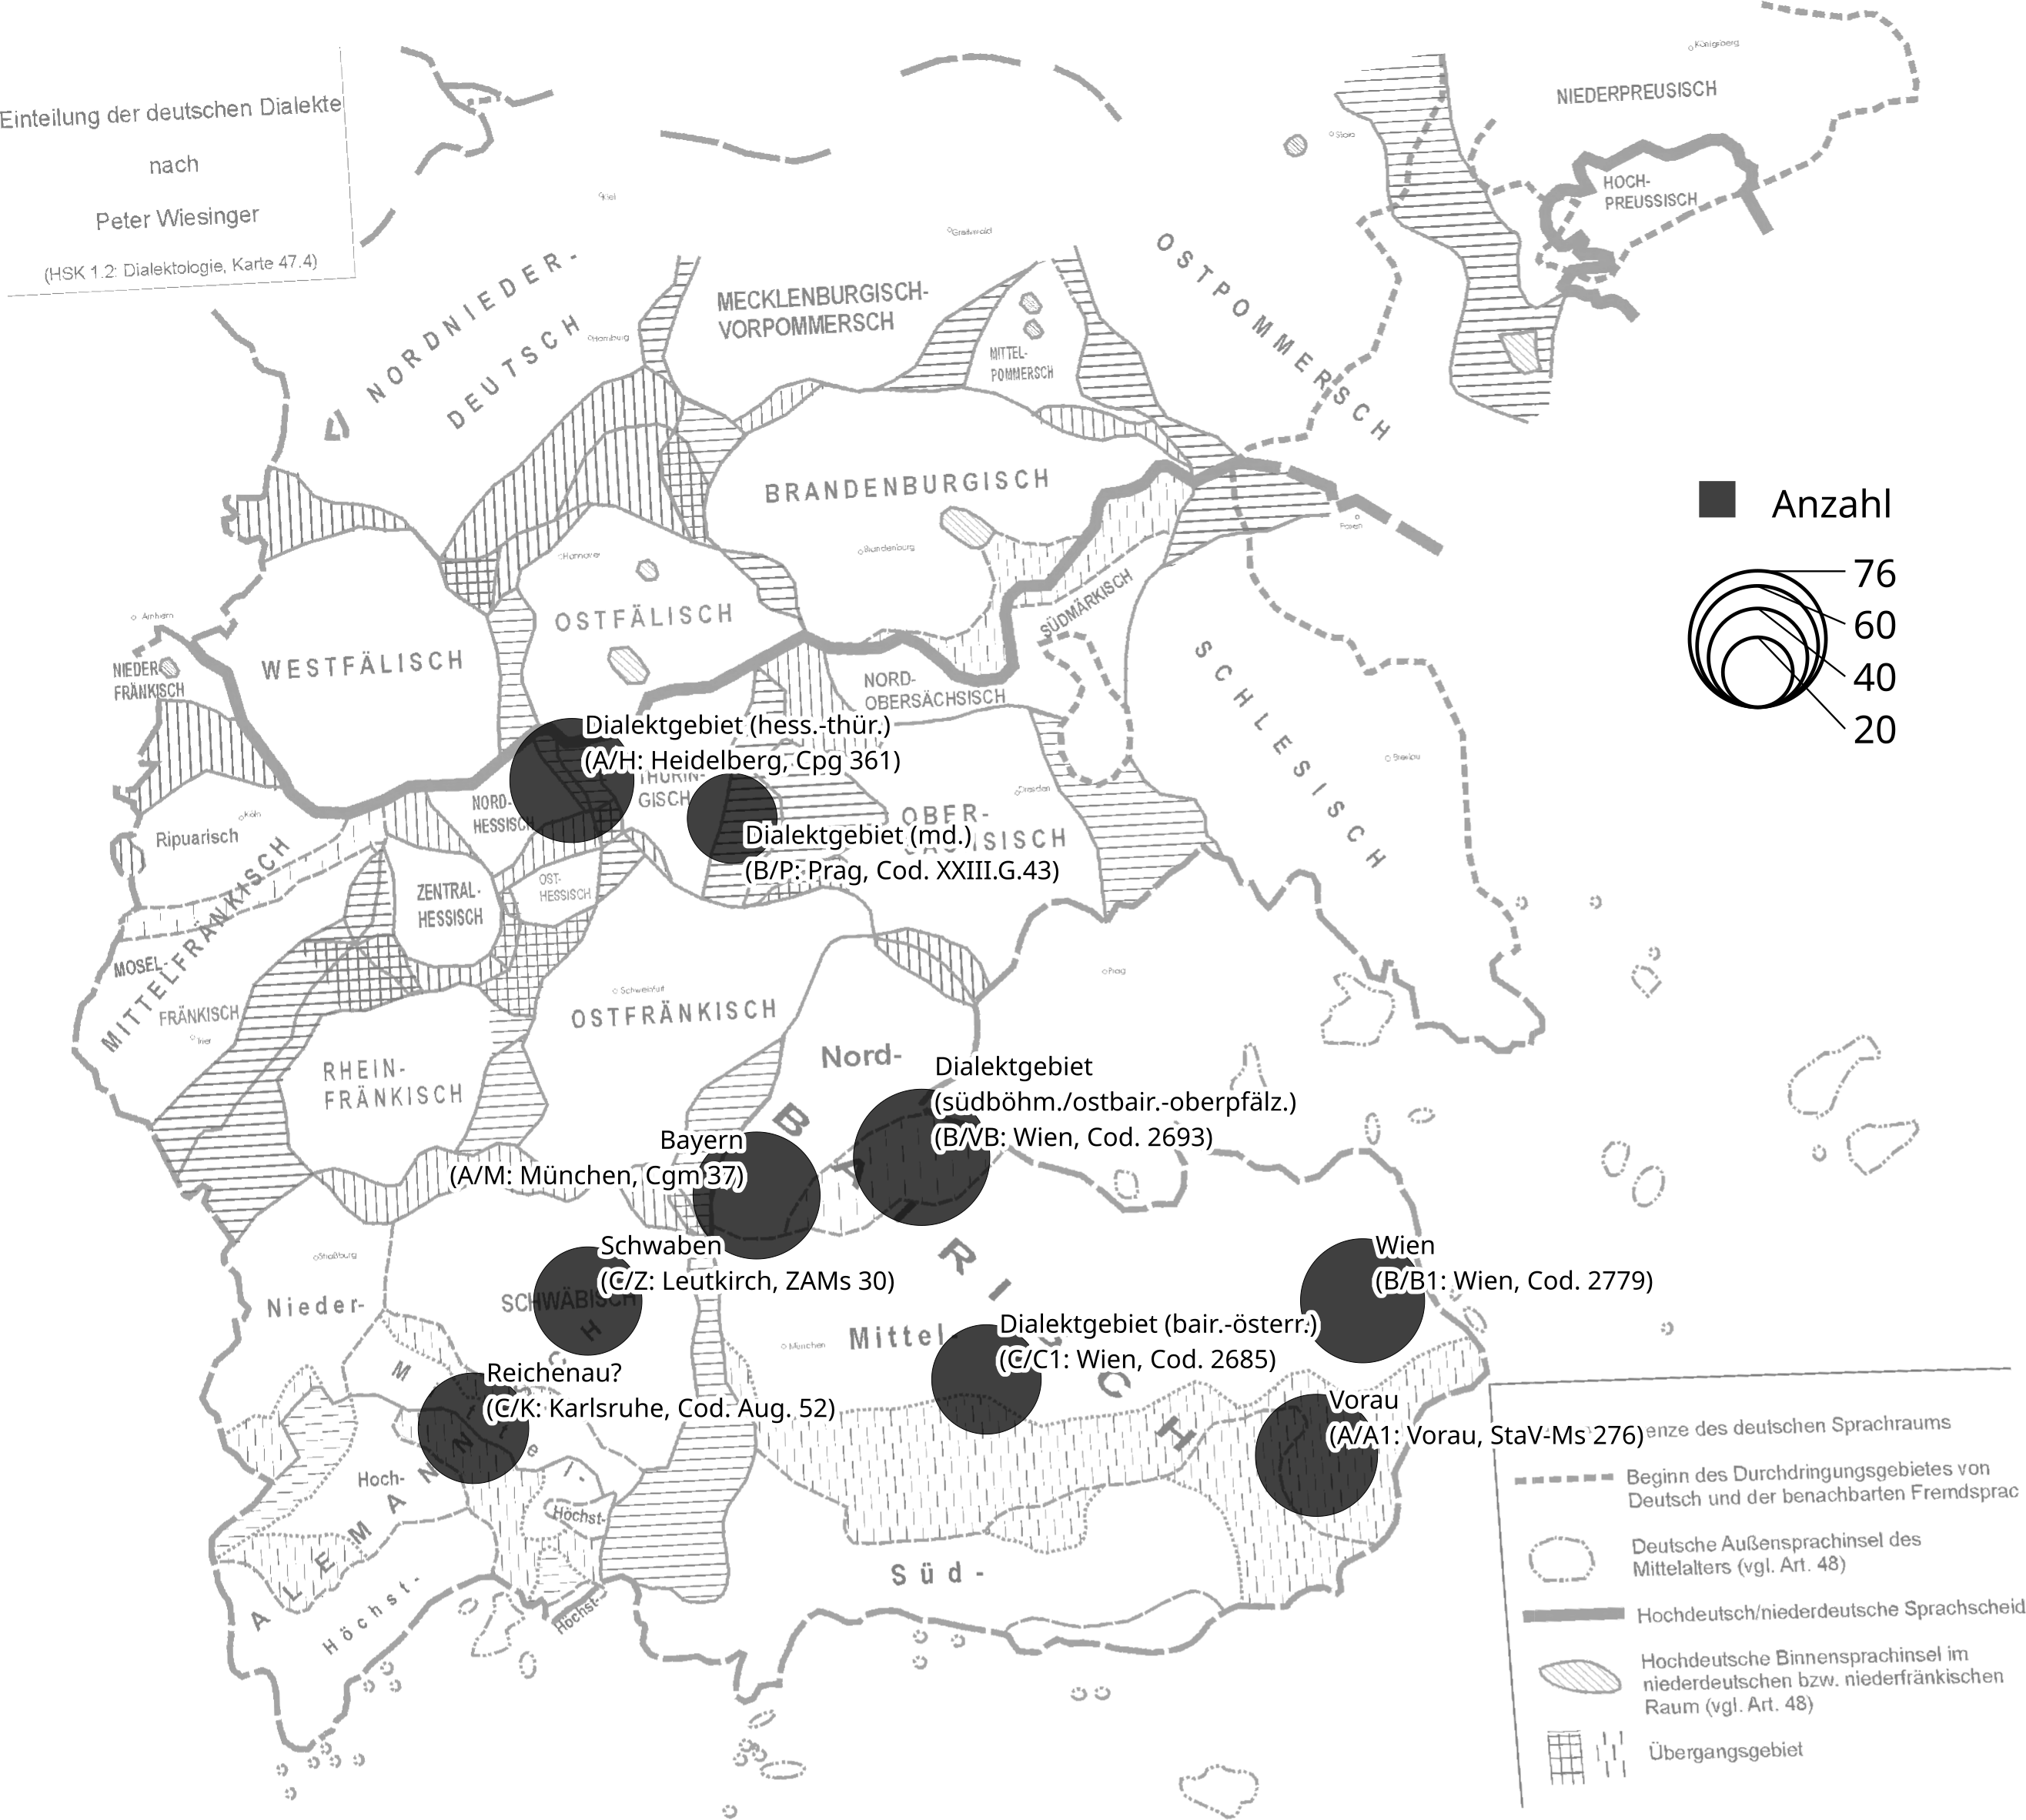
\includegraphics[
	width=\textwidth,
]{./figures/2022-03-07_belege_gebiet.png}
\caption[Anzahl der Belege für mhd.\ \norm{bėide} pro Sprachlandschaft und
Handschrift]{Anzahl der Belege für mhd.\ \norm{bėide} pro Sprachlandschaft
und Handschrift\nocite{wiesinger1983:rede}}
\label{fig:kartebelegzahl}
\end{figure}

Im Regelfall ist bei mittelalterlichen Handschriften keine genaue Einordnung in
Zeit und Raum möglich, da diese -- im Unterschied zu Urkunden -- oft keine
derartigen Selbstauskünfte bieten
\autocites[1309--1310]{wegera2000}[117--121]{bein2011}. Insofern sind bei
den Handschriften C1, H, M, P und VB nur weitläufige Regionen als
(dialekt-)geografische Bezugsgröße angegeben. Die Platzierung der
Handschriften auf der Karte folgt weitestgehend den Angaben des \citetitle{hsc}
\nosh\autocite{hsc} sowie den größtenteils deckungsgleichen Angaben in
\citet{kcdigital} und \citet{wolf:kckat}. Aufgrund der fehlenden Möglichkeit
einer genauen Ortszuweisung in den meisten Fällen haben die markierten Punkte
also lediglich Näherungscharakter und beanspruchen keinesfalls eine geografisch
exakte Festlegung auf den jeweiligen Kartenpunkt.

Darüber hinaus merkt \citet{klein1988} zur Handschrift H an, diese
Handschrift möge \textquote{zwar in Hessen entstanden sein},%
%
	\footnote{Der Terminus \q{Hessen} ist aufgrund der Geschichte des
	Bundeslandes ungenau. Dem Textzusammenhang nach wird wohl die
	Sprachlandschaft gemeint sein, die nicht deckungsgleich mit dem Territorium
	des modernen Bundeslandes ist \autocite[vgl.~z.\,B.][853]{wiesinger1983}.}
%
aber \blockcquote[118]{klein1988}{im thüringisch-hessischen Schreibdialekt
geschrieben und zeugt somit nicht für eine rheinische, sondern für eine
thüringisch-hessische \q{Kaiserchronik}\nocite{schroeder1895}-Rezeption}.
\textcites{kcdigital}[23]{wolf:kckat} geben mit
\citet[237--238]{millerzimmermann2007} vorsichtig \q{Hessen (Mainz?)} als
Entstehungsort an.
\phantomsection%
\label{phsec:vbherkunft}%
Darüber hinaus beobachtet \citeauthor{schneider1987} abweichend von den
Angaben im \citetitle{hsc} und \citet{kcdigital}, dass der Text der Handschrift
VB regelmäßig die eher für das Mitteldeutsche typische Kennform
\norm{quam} `kam' neben bairischem \norm{chom} enthält. Obwohl sie dem
Schreiber Bemühungen zur Vermeidung von Dialektismen attestiert, erwägt sie als
Entstehungsort den südböhmischen oder ostbairisch-oberpfälzischen Raum
\autocite[226]{schneider1987}.

Neben der räumlichen Dimension spielt bei sprachhistorischen Untersuchungen
auch der zeitliche Bezug eine Rolle. Textzeugen der \KC{} finden sich vom
letzten Viertel des 12.~Jahrhunderts (A1) bis ins späte
16.~Jahrhundert (T), wobei das Gros ins 13./14.~Jahrhundert fällt.
Die in der vorliegenden Untersuchung berücksichtigten Handschriften der
\KC{} entstanden zwischen dem letzten Viertel des 12.~Jahrhunderts und dem
Ende des 15.~Jahrhunderts, wie in \cref{fig:zeitstrahl} gezeigt. Die für die
Auswertung relevanten Textzeugen verteilen sich -- neben A1 aus dem
12.~Jahrhundert -- auf die beiden Jahrhundertviertel um 1300 und stehen damit
zeitlich den Urkunden des \CAO{} nahe.

\begin{figure}[p]
\centering
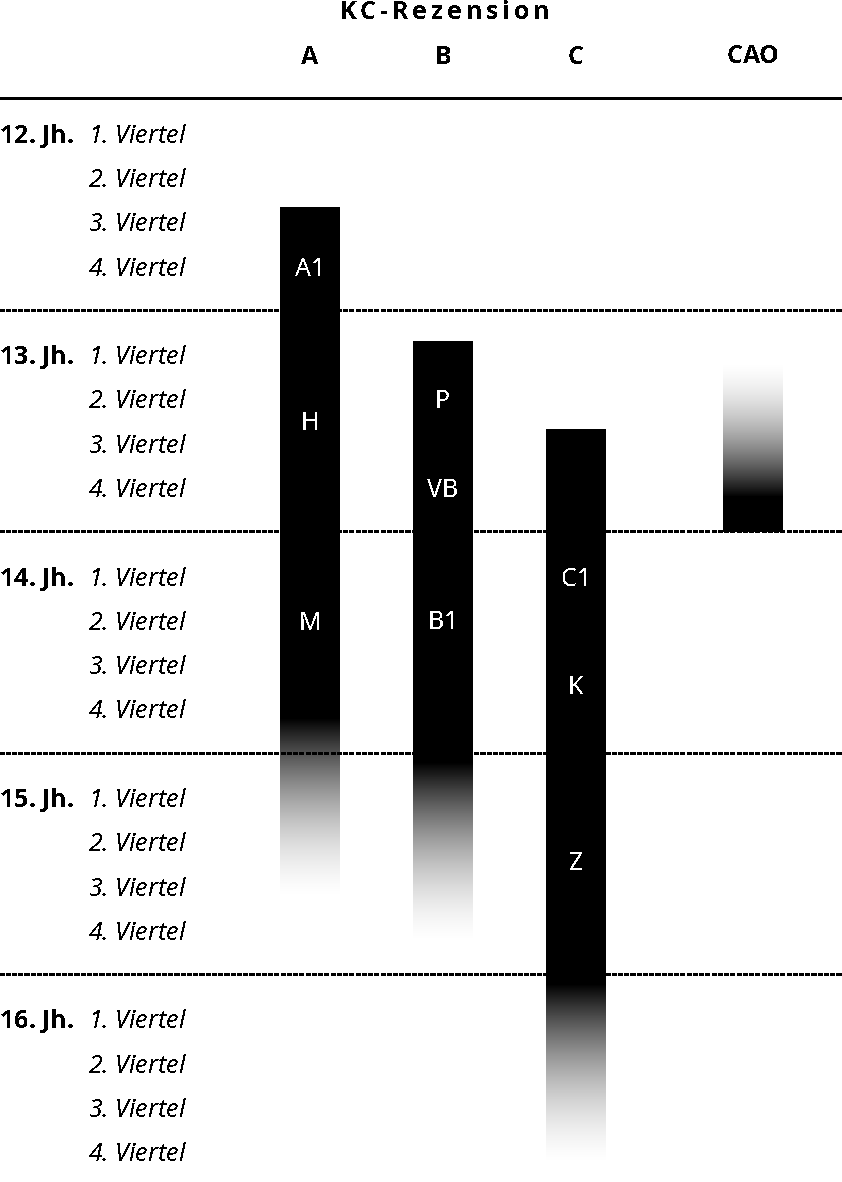
\includegraphics[
	height=.75\textheight,
]{./figures/ueberlieferungszeitraeume.pdf}
\caption{Zeitliche Verteilung der untersuchten Handschriften und Urkunden}
\label{fig:zeitstrahl}
\end{figure}

\section{Targets nach Personenmerkmalen des Controllers}
\label{sec:kctargpers}

\subsection{Nominale Controller}

Wie bei der Belegsammlung zum \CAO{} fällt die Belegmenge für den
direkten Bezug von \norm{bėide} auf zwei nominale Controller im ausgewerteten
\KC{}-Material gering aus. Für den hier untersuchten syntaktischen Kontext
liegen zwei Belege vor; zusammen mit der Kombination von Substantiv und
Pronomen sind es vier. Bei den zum Vergleich gesammelten Belegen zur direkten
Abhängigkeit von einzelnen Controllern im Plural finden sich dagegen 19
Beispiele.

\subsubsection{Kombinierte nominale Controller}
\label{subsubsec:conomctrlpers}

Das Beispiel in \cref{ex:beid2subst} und das Schema in \cref{fig:beid2subst}
verdeutlichen den syntaktischen Kontext, der im Folgenden zu untersuchen sein
wird. Der Quantor \norm{bėide} bezieht sich als Target direkt auf zwei
Controller, \lit{Willehalm} und \lit{Dietreich}, ohne dass eine Pronominalform
dazwischen steht.

\begin{exe}
\ex \label{ex:beid2subst}
	\gll Willehalm vnd Dietreich. \\
		Willehalm[\textsc{nom.sg.\MascM}] und Dietrich[\textsc{nom.sg.\MascM}] \\
\sn \gll wurden baíde da erſlagen. \\
		wurden beide-\textsc{nom.pl.\MascM.st} da erschlagen \\
	\trans `Willehalm und Dietrich wurden beide dort erschlagen.'
			(%
				C1:~83vb,36--37%
			)
\end{exe}

\begin{figure}
\begin{tikzpicture}[baseline=(1a_lb.base)]
	\node at (0,2)  (1a)    {\lit{Willehalm}};
	\node           (1a_box)[draw,rectangle,fit=(1a)] {};
	\node           (1a_lb) [above=.5ex of 1a_box, mynodefont]
	                        {controller 1};

	\node at (0,0)  (1b)    {\lit{Dietreich}};
	\node           (1b_box)[draw,rectangle,fit=(1b)] {};
	\node           (1b_lb) [above=.5ex of 1b_box, mynodefont]
	                        {controller 2};

	\node at (3,1) (2)      {\lit{baíde}};
	\draw (2) node (2_box)  [draw,rectangle,fit=(2)] {};
	\node (2_lb)   [above=.5ex of 2_box, mynodefont] {target};

	\draw [-latex] (1a_box) to [out=east, in=west] (2_box);
	\draw [-latex] (1b_box) to [out=east, in=west] (2_box);
\end{tikzpicture}
\caption{Direkter Bezug von \norm{bėide} auf zwei Controller}
\label{fig:beid2subst}
\end{figure}

Die erwähnten vier Belege mit einem \norm{bėide}-Target, das sich direkt auf
zwei Substantive bezieht, verteilen sich auf nur drei verschiedene
Parallelstellen. Die Menge an Kombinationen von Personenmerkmalen wird dadurch
stark reduziert. \cref{tab:koordnomctrl} gibt eine Übersicht über die Zahl der
Belege für den jeweiligen Flexionstyp und die zugehörige Kombination der
Personenmerkmale der Controller im hier besprochenen syntaktischen Kontext.

\begin{table}
\centering
\caption{Flexion nach Personenmerkmalen der kombinierten nominalen Controller}
\begin{tabular}{
	>{\scshape}l >{\scshape}l
	r r
	r
}
\toprule
\normalfont Controller 1
	& \normalfont Controller 2
	& \norm{bėide}
	& \norm{bėidiu}
	& Summe
	\\

\midrule

3sg.\MascM & 3sg.\MascM &  2 &  1  &  3 \\
3sg.\FemF  & 2sg\subM   &    &  1  &  1 \\

\midrule

\mc{2}{l}{Summe}          &  2 &  2  &  4 \\

\bottomrule
\end{tabular}
\label{tab:koordnomctrl}
\end{table}

Von den drei Belegen zur Kombination zweier maskulin-männlicher Referenten sind
zwei derselben Parallelstelle zugehörig: Der Beleg in \cref{ex:dietwill_2}
wurde eingangs zitiert, er sei hier noch einmal im Kontext seiner
Parallelstelle in \cref{ex:dietwill_3} wiedergegeben. Wie erwartet zeigt der
Quantor für diese Merkmalskombination die Form \norm{bėide} in allen Fällen.
Zur dritten Stelle mit \norm{bėidiu} siehe \cref{ex:babstimbaideu}.

\begin{exe}
\ex \label{ex:dietwill} % 203
	\begin{xlist}
	\ex \label{ex:dietwill_2}
		\gll Willehalm vnd Dietreich. \\
			Willehalm[\textsc{nom.sg.\MascM}] und Dietrich[\textsc{nom.sg.\MascM}] \\
	\sn \gll wurden baíde da erſlagen. \\
			wurden beide-\textsc{nom.pl.\MascM.st} da erschlagen \\
		\trans `Willehalm und Dietrich wurden beide dort erschlagen.'
			(%
				C1:~83vb,36--37%
			)

	\ex \label{ex:dietwill_3}
		\gll Wilhalm vnd dietrich \\
			Willehalm[\textsc{nom.sg.\MascM}] und Dietrich[\textsc{nom.sg.\MascM}] \\
	\sn \gll Wurden baide do erſlagen \\
			wurden beide-\textsc{nom.pl.\MascM.st} da erschlagen \\
		\trans `Willehalm und Dietrich wurden beide dort erschlagen.'
			(%
				K:~95vb,12--13%
			)
	\end{xlist}
\end{exe}

Beispiele für die Kombination von maskulin-männlichen und feminin-weib\-lichen
Substantiven ($\MascM+\FemF$, $\FemF+\MascM$) liegen im hier untersuchten
Kontext zumindest formal keine vor. Es gibt allerdings einen Einzelbeleg für
die Kombination von weiblicher und männlicher Referenz bei Substantiv und
Personal\-pronomen, der in \cref{ex:mutterdu} wiedergegeben wird.

\begin{exe}
\ex\label{ex:mutterdu}
	\gll Zvͦ dem chûnig ſprach er ſan \textelp{} \\
		zu dem König[\textsc{dat.sg.\MascM}] sprach er sodann {} \\
\sn \gll Dein muͦter vnd dv \\
		dein Mutter[\textsc{nom.sg.\FemF}] und \textsc{2sg\subM.nom} \\
\sn \gll Schv̂ln beideu chv̂men {dar zvͦ} \\
		sollen beide-\textsc{nom.pl.\NeutMF.st} kommen dahin \\
	\trans `Zum König sprach er sodann: \enquote{\textelp{} Deine
		Mutter und du sollt beide dahin kommen.}'
		(%
			B1:~23rc,5--14%
		)
\end{exe}

Hier verbirgt sich hinter dem \lit{dv} `du' trotz fehlender
Genusmarkierung beim Pronomen der 2.\ Pers.\ Sg.\ ein männlicher Referent,
nämlich der \lit{chûnig} `König', der direkt angesprochen wird. Der Beleg
passt damit in das Bild, das schon die Auswertung der Urkunden ergeben hat.
Auch bei Pro\-nomina ohne Genusmarkierung tritt aufgrund der referenzierten Personenmerkmale bei kombiniertem Bezug die
neutrale Form auf.

\phantomsection
\label{phsec:babstimbaideu}
Der Beleg in \cref{ex:babstimbaideu} mit \norm{bėidiu} in Bezug auf zwei
männliche Referenten wurde bereits erwähnt. Die Passage wurde hier so
interpretiert, dass sich \lit{ím} `ihm' auf \lit{Karle} `Karl (der
Große)' bezieht, also nicht auf \lit{wideme} `Dotierungen, Stiftungen'
\autocite[vgl. zur  Definition][s.\,v.~\fw{wideme}]{lexer:mhdhwb} und
\lit{zehende} `Zehnten'. Letzteres Wortpaar steht im Genitiv Plural
\autocite[vgl.][341]{paul2007}, sodass die erwartete Kongruenzform des
Quantors regelmäßig \norm{bėider(e)} `beider' lauten müsste. Andere Belege
mit \norm{bėidiu} als Genitivform wurden weder für diese Handschrift noch für
die anderen exzerpiert.%
%
	\footnote{In Bezug auf den Text der Edition von
	\citet{schroeder1895} übersetzt \citet[249]{mayer1874}:
	\blockquote{Als König Karl dann zu Gericht saß, trat der Pabst vor ihn hin
	und klagte, daß die Rechte, welche seinen Vorfahren seien verliehen worden,
	ihm von den Römern entrissen wurden, so seien ihm namentlich Zehenten und
	Widdume genommen}; vgl. auch \citet[83]{weis2022}.}

\begin{exe}
\ex\label{ex:babstimbaideu}
	\gll Karle an daz gerichte ſaz \\
		Karl[\textsc{nom.sg.\MascM}] an das Gericht saß \\
\sn \gll Der babſt klegt ím daz \\
		der Papst[\textsc{nom.sg.\MascM}] klagte \textsc{3sg.\MascM.dat} dass \\
\sn \gll Der wideme vnd der zehende gar \\
		der Dotierungen und der Zehnten gar \\
\sn \gll Waͤren baidu̍ worden bar \\
		wären beide-\textsc{nom.pl.\NeutM.st} geworden ledig \\
\sn \gll Von ſínen vorvarn \\
		von seinen Vorfahren \\
	\trans `Karl setzte sich zu Gericht. Der Papst klagte ihm, dass
		\textins{sie} beide an Dotierungen und gar an Zehnten ledig geworden
		wären durch seine Vorfahren.'
		(%
			K:~85vb,22--24; vgl. abweichend
			\KC:~V.~14383--14385;
			\cite[341]{schroeder1895}%
		)
\end{exe}

Erfahrungsgemäß sollte man vorsichtig sein, Erwartungen an die Grammatik
mittelhochdeutscher Texte zu stellen. Jedoch ist die Form \lit{beider} in
K ansonsten die für den Gen.\ Pl.\ regelmäßig belegte, wie die
Beispiele in \cref{ex:k_beider} zeigen, sodass davon ausgegangen werden kann,
dass sich \lit{baidiu} an dieser Stelle tatsächlich auf Karl und den Papst
bezieht.

\begin{exe}
\ex \label{ex:k_beider}
	\begin{xlist}
	\ex \label{ex:k_beider_1}
		\gll V̍nſer baider kínt \\
			unser beide-\textsc{gen.pl.st} Kind \\
	\sn \gll Bevilch ich allen die hie ſínt \\
			befehle ich allen die hier sind \\
		\trans `Unser beider Kind befehle ich allen an, die hier sind.'
			(%
				K:~9rb,25--26; vgl.
				C1:~8vb,27--28;
				% VC:~6va,13--14;
				Z:~31va,3--4; abweichend
				A1:~7va,3--4;
				H:~9va,42--43;
				P:~15va,14--15;
				\KC:~V.~1639;
				\cite[111]{schroeder1895}%
			)

	\ex \label{ex:k_beider_2}
		\gll In Rome bi ír baider zít \\
			in Rom bei ihr beide-\textsc{gen.pl.st} Zeit \\
	\sn \gll Huͦb ſich vrlu̍g vnd ſtrit \\
			hob sich Krieg und Kampf \\
		\trans `Zu ihrer beider Zeit erhoben sich in Rom Kampf und Krieg.'
			(%
				K:~28vb,36--37; vgl.
				% VC:~17va,31--32;
				Z:~93va,26--94ra,1; abweichend
				B1:~14va,49--50;
				VB:~24ra,30--31;
				P:~42ra,17--18;
				A1:~20vb,9--10;
				M:~36rb,6--7;
				H:~28rb,39--40;
				\KC:~V.~4837--4838;
				\cite[170]{schroeder1895}%
			)

	\ex \label{ex:k_beider_3}
		\gll Daz waz ír baider vngewín \\
			Das war ihr beide-\textsc{gen.pl.st} Verlust \\
		\trans `Das war ihr beider Verlust.'
			(%
				K:~103vb,27; vgl.
				C1:~91va,10;
				% VC:~60va,34;
				Z:~352ra,6;
				\KC:~V.~208;
				\cite[83]{schroeder1895}%
			)
	\end{xlist}
\end{exe}

\subsubsection{Einfache nominale Plural-Controller}
\label{subsubsec:nomctrlpers}

In diesem Abschnitt werden zum Vergleich Belege wie der in
\cref{ex:beidplsubst} angeführte und in \cref{fig:beidplsubst} illustrierte
diskutiert. Das Target \lit{bêde} `beide' ist hier ebenfalls unmittelbar auf
seinen Controller bezogen. Im Vergleich zum vorigen Abschnitt handelt es sich
beim Controller jedoch nicht um die Kombination von Substantiven, sondern nur
um ein einzelnes Substantiv, das im Plural steht.

\begin{exe}
\ex \label{ex:beidplsubst}
	\gll die gotes boten bêde \\
		 die Gottesboten[\textsc{nom.pl.\MascM}] beide-\textsc{nom.pl.\MascM.st} \\
	\trans `die beiden Gottesboten'
		(%
			\KC:~V.~7845;
			\cite[225]{schroeder1895}%
		)
\end{exe}

\begin{figure}
\begin{tikzpicture}[baseline=(1_lb.base)]
	\node (1)      [align=center]
	               {\lit{gotes boten}};
	\node (1_box)  [draw,rectangle,fit=(1)] {};
	\node (1_lb)   [above=.5ex of 1_box, mynodefont]{controller};

	\node (2)      [right=4em of 1_box, align=center]
	               {\lit{bêde}};
	\draw (2) node (2_box1) [draw,rectangle,fit=(2)] {};
	\node (2_lb1)  [above=.5ex of 2_box1, mynodefont] {target};

	\draw [-latex] (1_box) to (2_box1);
\end{tikzpicture}
\caption{Direkter Bezug eines Targets auf einen einzelnen Controller}
\label{fig:beidplsubst}
\end{figure}

Kontexte, in denen \norm{bėide} in einer direkten Kongruenzbeziehung mit einem
einzigen Substantiv im Plural steht, sind auch in der \KC{} im Vergleich
zu Kontexten mit kombinierter Referenz zahlreicher vorhanden.
\cref{tab:simpnomctrla} zeigt ihre Verteilung nach Personenmerkmalen und
Flexionstyp.

\begin{table}
\centering
\caption{Flexion nach Personenmerkmalen der einfachen nominalen Controller}
\begin{tabular}{>{\scshape}l r r r}
\toprule
\normalfont Controller
	& \norm{bėid(e)}
	& \norm{bėidiu}
	& Summe
	\\

\midrule

\MascM  & 11 &  2 & 13 \\
\NeutM  &    &  1 &  1 \\
\NeutA  &    &  1 &  1 \\

\midrule

\FemI   &  1 &    &  1 \\

\midrule

\normalfont Summe & 12 &  4 & 16 \\

\bottomrule
\end{tabular}
\label{tab:simpnomctrla}
\end{table}

Mit elf Belegen zu fünf Stellen verteilen sich die meisten
\norm{bėid(e)}-Formen mit maskulin-männlichem Bezug wie nach formalen Kriterien
erwartet \autocite[vgl.][182]{ksw2}. Interessant sind in diesem Kontext die
Abweichungen, das heißt, die zwei Belege für \norm{bėidiu} mit
maskulin-männlichem Bezug. Diese werden in \cref{ex:richtherriu} wiedergegeben.
Starke Adjektive zeigen in B1 ansonsten \norm{-iu} im Plural
regel\-mäßig nur bei den Neutra; Maskulina und Feminina sind dagegen stets
endungslos (vgl.~\cref{tab:kcadjdeclovw}).

\begin{exe}
\ex \label{ex:richtherriu}
	\begin{xlist}
	\ex \gll Die rihtær ſprachen beideu {dar zuͦ} \\
			die Richter[\textsc{nom.pl.\MascM}] sprachen beide-\textsc{nom.pl.\NeutM.st}
			dazu \\
		\trans `Die Richter äußerten sich beide dazu'
			(%
				B1:~28ra,8; vgl.~abweichend
				\KC:~V.~10090;
				\cite[267]{schroeder1895}% 1140 mit Parallelstelle in H
			)
		\label{ex:richtherriu_1}

	\ex \gll Die herren baten ir ſa \\
			Die Herren[\textsc{nom.pl.\MascM}] baten ihr alsbald \\
	\sn \gll Beideu beſvnder \\
			beide-\textsc{nom.pl.\NeutM.st} einzeln \\
		\trans `Die Herren hielten alsbald jeweils beide um ihre Hand an.'
			(%
				B1:~31va,48--49; vgl.
				\KC:~V.~11385--11386;
				\cite[289]{schroeder1895}% 1112x
			)
		\label{ex:richtherriu_2}
	\end{xlist}
\end{exe}

\phantomsection
\label{phsec:baideuwarn}
Der Beleg zu \norm{bėidiu} bei einem Neutrum mit männlichem Bezug in
\cref{ex:baideuwarn}, ein Parallelbeleg zu dem in \cref{ex:babstimbaideu}
zitierten, enthält formale Kongruenz. Das Lexem \lit{warn} `Kinder' zu
mhd.\ \norm{barn} `Kind, Sohn; Jüngling, Held (?)'
\autocites[s.\,v.\fw{barn}]{mwb1}[vgl.~auch][53]{kroonen2013} bezieht sich hier
metaphorisch auf Karl den Großen und Papst Leo~III., die vom Kaiserchronisten
als Brüder dargestellt werden (V.~14370;
\cites[341]{schroeder1895}[vgl.][83]{weis2022}). Obwohl sich \lit{warn} also
auf zwei erwachsene Männer bezieht, was die Wahrscheinlichkeit für semantische
Kongruenz erhöht (siehe \cref{sec:gendsex}), zeigt der Quantor in formaler
Übereinstimmung mit seinem Controller die neutrale Form.

\begin{exe}
\ex \label{ex:baideuwarn}
	\gll der wídem vnd der zehent gar. \\
		der Dotierungen und der Zehnten gar \\
\sn \gll wærn baidev warn bar. \\ % 1123
		wären beide-\textsc{nom.pl.\NeutM.st} Kinder[\textsc{nom.pl.\NeutM}] ledig \\
	\trans `an Dotierungen und Zehnten wären beide Kinder ledig'
		(%
			C1:~75rb,3--4; vgl.~abweichend
			K:~85vb,24;
			\KC:~V.~14384--14385;
			\cite[341]{schroeder1895}%
		)
\end{exe}

Auch der Quantor in \cref{ex:beideuher} dekliniert nach dem neutralen Genus
gemäß formaler Kongruenz innerhalb der Nominalphrase (NP). In
\cref{tab:simpnomctrla} wurde dieser Beleg mit \SA\ gekennzeichnet, da
\lit{her} `Heer' bei der Annotation als Committee Noun
\autocite[211--213]{corbett2006} aufgefasst wurde: Der Begriff, obwohl formal
im Singular, bezieht sich in seiner Semantik auf eine Gruppe von Menschen. In
jedem Fall zeigt sich nicht das Fehlen von overter Flexion, die ansonsten in
der Stichprobe zu B1 für den starken Nom./Akk.~Pl.~M./F. belegt ist.

\begin{exe}
\ex \label{ex:beideuher}
	\gll Der wær herre ûber beideu her \\
		der wäre Herr über beide-\textsc{acc.pl.\NeutA.st} Heer[\textsc{acc.pl.\NeutA}] \\
	\trans `Der wäre Herr über beide Heere'
		(%
			B1:~31rc,3; zu
			\KC:~V.~11272\,ff.;
			\cite[287]{schroeder1895}% 1110
		)
\end{exe}

Der Beleg für ein unbelebtes Femininum hat die Form \lit{baide}, insofern auch
hier der Quantor innerhalb der NP formale Kongruenz zeigt
\cref{ex:uozehende_2}, obwohl es sich um Körperteile handelt und damit um
etwas, von dem auszugehen ist, dass es eine mittlere Position zwischen den
Polen belebt und unbelebt einnimmt (vgl.~\cref{sec:gendsex} zur Annotation von
Genus bei Inanimata).

\begin{exe}
	\ex \gll Si wand ír baide hênde \\
			sie wand ihr beide-\textsc{acc.pl.\FemI.st} Hand-\textsc{acc.pl.\FemI} \\
		\trans `Sie wand ihre beiden Hände.'
			(%
				K:~6rb,19; vgl.
				\KC:~V.~913;
				\cite[98]{schroeder1895}%
			)
		\label{ex:uozehende_2}
\end{exe}

\subsubsection{Zusammenfassung}

Die Belegstellen zum kombinierten direkten Bezug von \mbox{\norm{bėide}} auf
zwei Substantive fallen nicht aus dem Rahmen bisheriger Ergebnisse, wenn es
auch die geringe Belegzahl unmöglich macht, generelle Aussagen zu treffen. In
beiden Fällen zeigte sich die Form \norm{bėide} mit Bezug auf maskuline und
feminine Referenten. Im Fall der Kongruenz eines Quantors mit einem einzelnen
Substantiv im Plural wiesen die Targets innerhalb der NP ebenfalls formale
Kongruenz auf, doch liegen zwei Belege für neutrales \norm{bėidiu} bei
eindeutig maskulin-männlichem Bezug vor.

\subsection{Anaphorische Controller}

Mit 19 Stellen liegt der größere Teil des Belegmaterials zur \KC{} für die
Kongruenzrelation zwischen \norm{bėide} in indirekter Abhängigkeit von zwei
nominalen Controllern vor. Die Kombination von Substantiv und einem Pronomen
der ersten oder zweiten Person als Diskurs\-anker wird hier mitgezählt.
Textstellen mit indirektem Bezug zwischen Quantor und einzelnem Substantiv im
Plural sind neun vorhanden.

\subsubsection{Indirekter Bezug auf kombinierte nominale Controller}
\label{subsubssec:iconomctrlpers}

Hier soll zunächst der Kongruenzbezug zwischen kombinierten Controllern und
Quantor mit einem Pronomen als Verbindungsglied anhand der gesammelten Belege
untersucht werden. Das Verhältnis zwischen Kongruenzcontrollern und Target wird
in \cref{ex:beidanactrl} und \cref{fig:beidanactrl} illustriert.%
%
	\footnote{Auch für die \KC{} gilt, dass das Personalpronomen der
		3.~Pers.\ Pl.\ Nom./Akk. in der Regel zu \norm{si} ausgeglichen
		erscheint, also keine Differenzierung zwischen maskulin-femininem
		\norm{sie} und neutralem \norm{siu} nachzuvollziehen ist, vergleiche
		\citet[213--214]{paul2007} und \citet[369, 390--397]{ksw2} sowie die
		Teiluntersuchung zur Form des Pronomens in
		\cref{subsubsec:monoflexionkc}.}

\begin{exe}
\ex\label{ex:beidanactrl}
	\gll Si nâmen di muoter mit dem sun, \\
		sie nahmen die Mutter[\textsc{acc.sg.\FemF}] mit dem Sohn[\textsc{dat.sg.\MascM}] \\
\sn \gll si viengen si bî dem hâre, \\
		sie fingen \textsc{3pl\subMF.acc} an dem Haare \\
\sn \gll si vuorten si baide zewâre \\
		sie führten \textsc{3pl\subMF.acc} beide-\textsc{acc.pl.m+f\subMF.st}
			wirklich \\
\sn \gll vur die burch an daz velt \\
		vor die Stadt an das Ebene \\
	\trans `Sie nahmen die Mutter mit dem Sohn. Sie fingen sie an den
		Haaren. Ja, sie führten sie beide vor die Stadt zu der Ebene.'
		(%
			KC:~V.~14269--14272;
			\cite[339]{schroeder1895}%
		)
\end{exe}

\begin{figure}
\begin{tikzpicture}[baseline=(1a_lb.base)]
	\node at (0,2)  (1a)    [gray]
	                        {\lit{muoter}};
	\node           (1a_box)[draw,gray,rectangle,fit=(1a)] {};
	\node           (1a_lb) [above=.5ex of 1a_box, gray, mynodefont]
	                        {controller 1};

	\node at (0,0)  (1b)    [gray]
	                        {\lit{sun}};
	\node           (1b_box)[draw,gray,rectangle,fit=(1b)] {};
	\node           (1b_lb) [above=.5ex of 1b_box, gray, mynodefont]
	                        {controller 2};    

	\node at (3,1) (2)      {\lit{si}};
	\draw (2) node (2_box1) [
	                    draw,
	                    gray,
	                    minimum height=3em,
	                    minimum width=3em,
	                    xshift=-.5ex,
	                    yshift=+.5ex,
	                    rectangle
	                ] {};
	\draw (2) node (2_box2) [
	                    draw,
	                    minimum height=3em,
	                    minimum width=3em,
	                    xshift=+.5ex,
	                    yshift=-.5ex,
	                    rectangle
	                ] {};
	\node           (2_lb1) [above=.5ex of 2_box1, gray, mynodefont]
	                        {target};
	\node           (2_lb2) [below=.5ex of 2_box2, mynodefont]
	                        {controller};

	\node at (6,1)  (3)      {\lit{baide}};
	\node           (3_box)  [draw,rectangle,fit=(3)] {};
	\node           (3_lb)   [above=.5ex of 3_box, mynodefont]
	                        {target};

	\draw [-latex,gray] (1a_box) to [out=east, in=west] (2_box1);
	\draw [-latex,gray] (1b_box) to [out=east, in=west] (2_box1);
	\draw [latex-]      (3_box)  to [yshift=1.5ex]      (2_box2);
\end{tikzpicture}
\caption{Indirekter Bezug eines Targets auf zwei \q{Erstcontroller} über ein Personalpronomen}
\label{fig:beidanactrl}
\end{figure}

Auch wenn es sich bei \lit{muoter mit dem sun} `Mutter mit dem Sohn' nicht
strikt um eine syntaktische Koordination vom Typ \q{X \fw{und}
Y} handelt (vgl.~\cref{sec:erwkonjbegr} zur \q{erweiterten}
Koordination), werden \lit{muoter} `Mutter' und \lit{sun} `Sohn'
durch \lit{si} `sie' kombiniert zusammengefasst. Der Quantor \lit{baide}
modifiziert dieses \lit{si} und kongruiert mit ihm. Der Quantor kongruiert
damit direkt mit dem Personalpronomen \lit{si} und indirekt mit \lit{muoter}
und \lit{sun}.

\Cref{tab:kcsimprefctrl} gibt die Belegverteilung in der \KC{} für die in
\cref{ex:beidanactrl} exemplarisch ausgeführte Kongruenzrelation wieder,
wobei auch hier nur Handschriften berück\-sichtigt wurden, die beide
Kongruenzformen aufweisen (effektiv: B1 und VB; vgl.~auch
\cref{sec:adjdeclkc} zur Adjektivdeklination in \KC{}-Handschriften).

\begin{table}
\centering
\caption{Flexion nach Personenmerkmalen der anaphorischen Controller
(kombinierter Bezug)}
\begin{tabular}{
	>{\scshape}l @{$~+~$} >{\scshape}l
    r r
    r
}
\toprule
\mc{2}{c}{Controller}
    & \norm{bėid(e)}
    & \norm{bėidiu}
    & Summe
    \\

\midrule

% Controller              | e  | iu | Σ
3sg.\MascM & 3sg.\MascM & 11 &  1 & 12 \\

\midrule

1sg\subF & 2sg\subX     &  1 &  1 &  2 \\
2sg\subM & 1sg\subF     &    &  1 &  1 \\
2sg\subM & 3sg.\FemF    &    &  1 &  1 \\

\midrule

\mc{2}{l}{Summe}          & 12 &  4 & 16 \\

\bottomrule
\end{tabular}
\label{tab:kcsimprefctrl}
\end{table}

In \cref{tab:kcsimprefctrl} entfällt textbedingt der größte Anteil auf die
Kombination zweier maskulin-männlicher Referenten ($3sg.\MascM +
3sg.\MascM$). Insgesamt weisen 14 von 16 Belegen (zu zwölf Textstellen) die zu
erwartende Flexionsform auf. Bei den zwei übrigen Belegen handelt es sich um
einen Beleg vom Typ \norm{bėide} mit Bezug auf zwei Neutra sowie einen Beleg
für \norm{bėidiu} bei kombinierten Maskulina.

Für die vorliegende Untersuchung am interessantesten ist das Belegpaar zur 1.\
Pers.\ Sg. (weiblich) in Kombination mit einer 2.\ Pers.\ Sg.: An der
betreffenden Stelle spricht ein \norm{wīp} `Frau' zu seinem
\norm{kindelīn} `Kindlein' (V.~910--932; \cite[98]{schroeder1895}). Das
Geschlecht des Kindes ist unbekannt; es muss sich dem Kontext nach um einen
Säugling handeln. Die beiden Belegstellen werden in \cref{ex:wipkindelin}
wiedergegeben.

\begin{exe}
\ex \label{ex:wipkindelin}
	\begin{xlist}
	\ex \label{ex:wipkindelin_1}
		\gll Sit wír nv mvͤzzen verderben \\
			da \textsc{1pl\tsub{\SF/\SX}.nom} nun müssen zugrunde.gehen \\
	\sn \gll Vnd beide von den heiden ſterben \\
			und beide-\textsc{nom.pl.m+f\tsub{\SF/\SX}.st} von den Heiden
				sterben \\
		\trans `Da wir (jetzt) wohl zugrunde gehen werden und beide durch die Heiden sterben.'
			(%
				VB:~5rb,33--34; vgl.~abweichend
				\KC:~V.~931--932;
				\cite[98]{schroeder1895}%
			)
		
	\ex \label{ex:wipkindelin_2}
		\gll Seit wir muͤzzen verderben. \\
			da \textsc{1pl\tsub{\SF/\SX}.nom} müssen zugrunde.gehen \\
	\sn \gll und beideu von den haiden ſterben \\
			und beide-\textsc{nom.pl.n\tsub{\SF/\SX}.st} von den Heiden
				sterben \\
		\trans `Da wir (jetzt) wohl zugrunde gehen werden und beide durch die Heiden sterben.'
			(%
				B1:~4vb,57--58; vgl.~abweichend
				\KC:~V.~931--932;
				\cite[98]{schroeder1895}%
			)
	\end{xlist}
\end{exe}

In der Klassifikation in \cref{tab:kcadjdeclovw} gehört VB zur
Gruppe 3. Das bedeutet, dass in der Stichprobe zur Adjektiv\-flexion leichte
Variation zwischen \norm{-iu} und \norm{-e} im Plural Neutrum vorliegt, wobei
\norm{-iu} überwiegt. Um einen solchen Fall mag es sich auch hier handeln.
Daneben besteht die Möglichkeit, dass in \cref{ex:wipkindelin_1} der generellen
Belebtheit der Controller wegen die Form \lit{beide} auftritt. Die Form
\lit{beideu} in \cref{ex:wipkindelin_2} passt zum einen zur Kombination von
zwei formalen Neutra, zum anderen als Resolutionsform, insofern weiblich und
\q{unspezifisch} keine Schnittmenge besitzen
(vgl.~\cref{subsubsec:x+x_dir_anim} zur theoretischen Modellierung der
Kombination von Genusmerkmalen).

Der andere oben genannte Beleg mit \norm{bėidiu} statt regelhaftem \norm{bėide}
bei der Kombination zweier Maskulina wird in \cref{ex:papstkoenig} angeführt.
Die \norm{iu}-Form des Quantors bei kombiniertem männlichen Bezug ist
irregulär. % (vgl.~\cref{subsec:m+m_anim_beidiu}).

\begin{exe}
\ex\label{ex:papstkoenig} % 224
	\gll Der papſt vnd der chv̂nich \\
		der Papst[\textsc{nom.sg.\MascM}] und der König[\textsc{nom.sg.\MascM}] \\
\sn \gll Si warn zegot biderb vnd frumic \\
		\textsc{3pl\subM.nom} waren {zu=Gott} brav und tüchtig \\
\sn \gll Zegot ſtuͦnt allr ir geſín \\
		{zu=Gott} stand aller ihr Sinnen \\
\sn \gll Beideu ſchatz vnd gewín \\
		beide Schatz und Gewinn \\
\sn \gll Liezzen ſi beideu gelich \\
		ließen \textsc{3pl\subM.nom} beide-\textsc{nom.pl.\NeutM.st} gleich \\
	\trans `Der Papst und der König, sie waren Gott gegenüber brav und
		tüchtig. Auf Gott war all ihr Sinnen gerichtet. Sowohl Schatz als auch
		Gewinn war ihnen beiden gleich.'
		(%
			B1:~17vb,30--34; vgl.~abweichend
			\KC:~V.~6110--6113;
			\cite[202]{schroeder1895}%
		)
\end{exe}

Sowohl bei \lit{ſchatz} `Schatz' als auch bei \lit{gewín} `Gewinn'
handelt es sich um unbelebte Maskulina. Es scheint im Kontext der Stelle
sinnvoller, das neutrale \lit{beideu} in Zeile~34 nicht darauf, sondern auf
\lit{ſi} -- den \lit{papſt} `Papst' und den \lit{chv̂nich} `König' --
zu beziehen. Der Blick in die Parallelstellen in VB und
A1 stützt diese Interpretation, insofern es hier trotz abweichendem
Wortlaut eindeutig um das gottgefällige Handeln von Kaiser Philippus und Papst
Sixtus geht \cref{ex:papstkoenig2}.

\begin{exe}
\ex\label{ex:papstkoenig2}
\begin{xlist}
	\ex \label{ex:papstkoenig2_1}
		\gll Beidiv ſchatz vnd gewín \\
			beide Schatz[\textsc{acc.sg.\MascI}] und Gewinn[\textsc{acc.sg.\MascI}] \\
	\sn \gll Liezzen ſie gelíche. \\
			ließen \textsc{3pl\subM.nom} gleich \\
		\trans `Sowohl Schatz als auch Gewinn war ihnen gleich.'
			(%
				VB:~29vb,38%
			)

	\ex \label{ex:papstkoenig2_2}
		\gll baidiv ſcaz unde gewin. \\
			beide Schatz[\textsc{acc.sg.\MascI}] und Gewinn[\textsc{acc.sg.\MascI}] \\
	\sn \gll liezen ſi in beſlifen. \\
			ließen \textsc{3pl\subM.nom} \textsc{refl.dat.pl\subM} entgehen \\
		\trans `Sowohl Schatz als auch Gewinn ließen sie sich entgehen'
			(%
				A1:~26rb,40--41; vgl.
				H:~36ra,40--41;
				\KC:~V.~6112--6113;
				\cite[202]{schroeder1895}%
			)
\end{xlist}
\end{exe}

Für den kombinierten Bezug auf Personen von eindeutig unterschiedlichem
Geschlecht liegt zumindest ein einziger Beleg vor. Die Kombination von 2.\
Pers. Sg.\ (männlich) und 1.\ Pers.\ Sg.\ (weiblich) wird durch
\norm{bėidiu} aufgenommen, womit Gender Resolution vorliegt: \lit{so wærn wir
baidev verloͤrn} `dann wären wir beide verloren' (C1:~60rb,44--60va,3).

\subsubsection{Indirekter Bezug auf unkombinierte Plural-Controller}
\label{subsubsec:beid2p2snglnkc}

Beim indirekten Bezug zwischen einem einzelnen Substantiv im Plural und
\norm{bėide} als Target wie in \cref{ex:nplsibeide} und \cref{fig:nplsibeide}
liegt in der Stichprobe zur \KC{} keine Variation vor. In allen neun Fällen
sind ausschließlich Formen von \norm{bėid(e)} belegt, davon besitzen alle eine
männlich-maskuline Referenz.

\begin{exe}
\ex \label{ex:nplsibeide}
	\gll do die hêrren pranten \textelp{} \\
			als die Herr-\textsc{nom.pl.\MascM} brannten {} \\
\sn \gll da ze Kastel er si baide begraif \\
			dort zu Kastel er \textsc{3pl\subM.acc}
			beide-\textsc{acc.pl.\MascM.st} ergriff \\
		\trans `Als die Herren brandschatzten \textelp{} Dort in Kastel ergriff
			er sie beide'
			(%
				\KC:~V.~16104--16111;
				\cite[372]{schroeder1895}%
			)
\end{exe}

\begin{figure}
\begin{tikzpicture}[baseline=(2_lb1.base)]
    \node at (0,0)  (1)     [gray]
                            {\lit{hêrren}};
    \node           (1_box) [draw,gray,rectangle,fit=(1)] {};
    \node           (1_lb)  [above=.5ex of 1_box, gray, mynodefont]
                            {controller};

	\node at (3,0) (2)      {\lit{si}};
    \draw (2) node (2_box1) [
                        draw,
                        gray,
                        minimum height=3em,
                        minimum width=3em,
                        xshift=-.5ex,
                        yshift=+.5ex,
                        rectangle
                    ] {};
    \draw (2) node (2_box2) [
                        draw,
                        minimum height=3em,
                        minimum width=3em,
                        xshift=+.5ex,
                        yshift=-.5ex,
                        rectangle
                    ] {};
    \node           (2_lb1) [above=.5ex of 2_box1, gray, mynodefont]
                            {target};
    \node           (2_lb2) [below=.5ex of 2_box2, mynodefont]
                            {controller};

    \node at (6,0)  (3)      {\lit{baide}};
    \node           (3_box)  [draw,rectangle,fit=(3)] {};
    \node           (3_lb)   [above=.5ex of 3_box, mynodefont]
                            {target};

    \draw [-latex,gray] (1_box)  to [yshift=-1.5ex]     (2_box1);
    \draw [latex-]      (3_box)  to [yshift=1.5ex]      (2_box2);
\end{tikzpicture}
\caption{Indirekter Bezug eines Targets auf einen einzelnen \q{Erstcontroller} über ein Personalpronomen}
\label{fig:nplsibeide}
\end{figure}

\subsubsection[Zu Askedals (1973) Hypothese der
‚Monoflexion‘]{Zu \posscite{askedal1973} Hypothese der \q{Monoflexion}}
\label{subsubsec:monoflexionkc}

Bezüglich \posscite{askedal1973} Hypothese zur \q{Monoflexion}
(vgl.~\cref{subsubsec:monoflexioncao} zur Situation im \CAO{}) ist in
den \KC{}-Handschriften, die für diese Analyse ausgewertet wurden, nur
sehr wenig Variation zwischen \norm{bėide} und \norm{bėidiu} anzutreffen. Die
Kombination vom Typ \norm{si bėide} ist in allen Handschriften, bei denen
sowohl \norm{bėide} als auch \norm{bėidiu} als Quantor auftritt (B1,
C1, K und VB; vgl.~\cref{tab:beidevar}) mit
Ausnahme einer Stelle in B1 die einzig belegte. Belege mit
Relativpronomen als Controller liegen lediglich drei vor, die sich auf zwei
Stellen beziehen.

\begin{table}
\centering
\caption{Kombinationen von \norm{si/sie/siu} und \norm{di/die/diu} mit \norm{bėide/-iu} in der \KC{}}
\begin{tabular}{
	l
	@{\hspace{4\tabcolsep}}
	r
	r
	@{\hspace{4\tabcolsep}}
	r
	@{\hspace{4\tabcolsep}}
	r
}
\toprule

Controller
	& \norm{bėide}
	& \norm{bėid}
	& \norm{bėidiu}
	& Summe
	\\

\midrule

\norm{si}  & 12 &  6 &  1 & 19 \\

\midrule

\norm{di}  &  1 &  1 &    &  2 \\
\norm{die} &  1 &    &    &  1 \\

\midrule

Summe      & 14 &  7 &  1 & 22 \\

\bottomrule
\end{tabular}
\label{tab:siebeidevar}
\end{table}

Weshalb in dem Beleg in \cref{ex:papstkoenig3}, der auch an dieser Stelle
relevant ist, \norm{bėidiu} auftritt, ist nicht eindeutig nachvollziehbar, da
es an dieser Stelle um zwei Männer geht, nämlich den Papst und den König. In
\cref{phsec:babstimbaideu} wurde zur Merkmalskombination im vorliegenden
syntaktischen Kontext argumentiert, dass der Bezug von \lit{beideu} auf das
Figurenpaar dem Kontext nach wahrscheinlicher ist als auf \lit{ſchatz vnd
gewín} `Schatz und Gewinn', auch wenn letzteres nicht hundertprozentig
ausgeschlossen werden kann.

\begin{exe}
\ex\label{ex:papstkoenig3} % 224
	\gll Der papſt vnd der chv̂nich \\
		der Papst[\textsc{nom.sg.\MascM}] und der König[\textsc{nom.sg.\MascM}] \\
\sn \gll Si warn zegot biderb vnd frumic \\
		\textsc{3pl\subM.nom} waren {zu=Gott} brav und tüchtig \\
\sn \gll Zegot ſtuͦnt allr ir geſín \\
		{zu=Gott} stand aller ihr Sinnen \\
\sn \gll Beideu ſchatz vnd gewín \\
		beide Schatz und Gewinn \\
\sn \gll Liezzen ſi beideu gelich \\
		ließen \textsc{3pl\subM.nom} beide-\textsc{nom.pl.\NeutM.st} gleich \\
	\trans `Der Papst und der König, sie waren Gott gegenüber brav und
		tüchtig. Auf Gott war all ihr Sinnen gerichtet. Sowohl Schatz als auch
		Gewinn war ihnen beiden gleich.'
		(%
			B1:~17vb,30--34; vgl.~abweichend
			\KC:~V.~6110--6113;
			\cite[194]{schroeder1895}%
		)
\end{exe}

Zwei Belege für \norm{sie bėide} liegen in VB (21ra,25--31 und
22ra,34--22rb,6) vor; dazu V.~4255--4261 und abweichend V.~4455--4470
\autocite[159, 163]{schroeder1895}. Jedoch steht \norm{bėide} in beiden dieser
Fälle im Reim, sodass hier ohnehin nicht mit Variation bei der Flexion des
Quantors zu rechnen ist und die Belege daher nicht in die bereinigte Stichprobe
eingeflossen sind. In den Handschriften A1 und M, die bei dieser
Detailauswertung ansonsten nicht berücksichtigt wurden, liegt zu einer Stelle
jeweils die Kombination \norm{siu bėide} vor \cref{ex:siubedea1m}. Hier bezieht
sich der Quantor indirekt auf ein eindeutig maskulin-männliches Substantiv im
Plural: \norm{jungere} `Jünger'. Die Belege für \lit{bede} stehen dabei jedoch
ebenfalls im Reim und damit in einer Neutralisierungsposition
\autocites[vgl.][662--663]{grimm1870}[89]{askedal1973}.

\begin{exe}
\ex \label{ex:siubedea1m}
	\begin{xlist}
	\ex \label{ex:siubedea1m_1}
		\gll er nam ſiner iungere zuene. \\
			er nahm seiner Jünger[\textsc{gen.pl.\MascM}] zwei[\MascM] \\
	\sn \gll er ſante ſiv dar bede. \\
			er sandte \textsc{3pl\subM.acc} fort beide-\textsc{acc.pl.\MascM.st} \\
		\trans `Er nahm zwei seiner Jünger. Er sandte sie beide fort.'
			(%
				A1:~16vb,28--29; vgl.
				\KC:~V.~3937--3938;
				\cite[153]{schroeder1895}%
			)
	
	\ex \label{ex:siubedea1m_2}
		\gll Er nam ſíner ivnger zwene. \\
			er nahm seiner Jünger[\textsc{gen.pl.\MascM}] zwei[\MascM] \\
	\sn \gll Er ſant ſiv dar bede. \\
			er sandte \textsc{3pl\subM?.acc} fort beide-\textsc{acc.pl.\MascM.st} \\
		\trans `Er nahm zwei seiner Jünger. Er sandte sie beide fort.'
			(%
				M:~29va,18--19; vgl.
				\KC:~V.~3937--3938;
				\cite[153]{schroeder1895}%
			)
\end{xlist}
\end{exe}

Wie bei der Diskussion der \CAO{}-Belege in demselben Kontext
erörtert, ist die Form \norm{siu} mit persönlicher Referenz ein Merkmal vor
allem des Alemannischen \autocite[vgl.][395]{ksw2}. Auch \lit{bede} kommt
hauptsächlich in Straßburger Urkunden sowie im hier ausgeklammerten
mitteldeutschen Sprachraum vor. Irritierend ist, dass A1 und
M dem bairischen Sprachraum zugeordnet werden
\autocites{wolf:kckat}[266--276]{fleischer2019}.%
%
	\footnote{Auch wenn \citet[40--41]{schneider1987} insgesamt zu dem Schluss
		kommt, dass der \KC{}-Text in A1 bairische Merkmale
		aufweist, bemerkt sie, dass keine eindeutige sprachliche Einordnung der
		Handschrift als solche möglich sei, da
		\blockquote[{\cite[40]{schneider1987},
		vgl.~\nosh\cites[519]{gaertner1999}[1638]{2vl11}}]{die einzelnen
		Dichtungen bzw.\ Textgruppen ganz unterschiedliche sprachliche
		Kriterien auf\textins{weisen}, \textelp{} auch verschiedene zeitliche
		Sprachstufen wieder\textins{spiegeln} \textins{sic}}.%
	}
%
Die Frage ist also, inwiefern diese Formen in einen bairischen Schreib\-kontext
passen.

\citet[396--397]{ksw2} führen \norm{seu} (mit neuhochdeutscher
Diphthongierung) als ver\-all\-gemeinerte Form des Nom./Akk.\ Pl.\ im
Bairischen an und mutmaßen, dass diese Form in der Umgebung des Habsburgers
Albrecht~I.\ (1255--1308) aus dem Alemannischen entlehnt worden sein könnte.
Indes wird A1 dem 12.~Jahrhundert zugeordnet
\autocite{kcdigital,wolf:kckat}. Die Form \lit{bede} `beide' kommt in
A1 neben \lit{bediu}, \lit{bæde} und \lit{bædiu} vor -- anders als
in Straßburger Urkunden ist der Quantor also nicht starr.
\citeauthor{wiesinger2001} interpretiert die Schreibung von mittelhochdeutsch
\norm{ėi} als \lit{e} als \blockcquote[103]{wiesinger2001}{häufige
mono\-graphische Variante \textelp{} im 12.\ und 13.~Jahrhundert}.

Die Belegverteilung von \norm{bėide} und \norm{bėidiu} weist in beiden
Handschriften, A1 und M, eine Trennung in \norm{bėide} als Quantor und
\norm{bėidiu} als Konjunktion auf, was allerdings auch daran liegen könnte,
dass für den Quantor nahezu ausschließlich männliche beziehungsweise maskuline
Referenten vorliegen. Anzumerken ist, dass die Form \norm{bed-} in A1 nur bis
Bl.~33vb belegt ist, also nur für die erste Hälfte des Texts. In M kommt
\norm{bed-} dagegen nur als Quantor vor, und in diesen Fällen nur mit \norm{-e}
oder -Ø.

Zuvor wurde festgestellt, dass im Belegmaterial zur \KC{} nur
\norm{si} in Kombination mit \norm{bėide} auftritt. Die Frage drängt sich
auf: Wie sieht es im Vergleich dazu mit regulären Vorkommen von `sie' aus?
Da die \KC{}-Hand\-schrif\-ten in der vorliegenden Form nicht
morphologisch annotiert sind, ist es nicht möglich, automatisiert nach Formen
des Personal\-pronomens der 3.~Pers.\ Pl.\ Nom./Akk.\ zu suchen, ohne dabei
potenzielle Falschpositive zur 3.~Pers.\ Sg.~F.\ Nom./Akk.\ oder zu \norm{sī}
als 1./3.~Pers.\ Sg.\ Konj.\ Präs.\ von \norm{sīn} `sein' zu erhalten. Um
die Menge der Belege eines so frequenten Lexems dennoch handhabbar zu machen,
wurden eintausend zufällig ausgewählte Zeilen der einzelnen in
\cref{tab:sieprn} aufgeführten Textzeugen ausgezählt. Dieses Vorgehen
gewährleistet, dass die Belege der Stichprobe aus thematisch unterschiedlichen
Episoden stammen, über den gesamten Text gestreut und damit repräsentativ sind.
Vorkommen von \norm{si} als Basis für ein Enklitikum (\norm{siȥ/-n} $\gets$
\norm{si eȥ/in} `sie es/ihn',
\norm{sine} $\gets$ \norm{si ne} `sie \textsc{neg}') wurden dabei nicht gezählt.

\begin{table}
\centering
\caption{Varianten des Personalpronomens der 3.\ Pers.\ Pl.\ Nom./Akk.\ in je 1.000 Zeilen}
\begin{tabular}{l
	r
	@{\hspace{4\tabcolsep}}
	r r r
	@{\hspace{4\tabcolsep}}
	r
}
\toprule
Hs.
	& \norm{si}
	& \norm{sie}
	& \norm{siu}
	& \norm{sei}
	& Summe
	\\

\midrule

A1
	& 123
	& 2
	& 1
	& % --
	& 126
	\\

M
	& 86
	& % --
	& 6
 	& 2
	& 94
	\\

\midrule

B1
	& 83
	& 1
	& % --
	& 2
	& 86
	\\

VB
	& 37
	& 38
	& % --
	& % --
	& 75
	\\

\midrule

C1
	& 97
	& % --
	& % --
	& % --
	& 97
	\\

K
	& 50
	& % --
	& % --
	& % --
	& 50
	\\

\midrule

Summe
	& 476
	&  41
	&   7
	&   4
	& 528
	\\

\bottomrule
\end{tabular}
\label{tab:sieprn}
\end{table}

In \cref{tab:sieprn} fällt die Häufung von \norm{si} bei allen Handschriften
außer VB auf -- hier kommen \norm{si} und \norm{sie} nahezu
gleich häufig vor und vor allem völlig parallel zueinander \cref{ex:vbsisie}.%
%
	\footnote{Auffällig ist auch, dass \lit{bi} und \lit{bie} für mhd.\
	\norm{bī} `bei' nebeneinander auftreten.
	Allerdings findet sich im \CAO{} die Grafie \lit{ie, iͤ} für
	mhd.~\norm{ī} im Bairischen allgemein
	\autocite[2910--2911]{reiffenstein2003}, zum Beispiel in Salzburg und
	Brixen, weit abseits des mitteldeutschen Sprachraums
	\autocites[24--25]{becker2013}[vgl.][248]{wmu1}[1231]{wmu2}.}
%
In C1 und K tritt das Pronomen dagegen allein in der Form
\norm{si} auf. Aufgrund der alemannischen Schreibsprache von K wäre
unbelegtes *\lit{ſu̍} neben belegtem \lit{du̍} als Vertreter von
genusindifferentem \norm{siu} zumindest denkbar.

\begin{exe}
\ex \label{ex:vbsisie}
 	\begin{xlist}
 	\ex \gll Von got ſi den gewalt haten \\
		     von Gott \textsc{3pl\subM.nom} den Macht hatten \\
 	\sn \gll Daz ſie chvcten die toten \\
		     dass \textsc{3pl\subM.nom} schauten die Toten \\
		\trans `Von Gott hatten sie \textins{=~die Herren} die Macht, die
			Toten zu schauen.'
			(%
				VB:~42ra,38--39; vgl.
				\KC:~V.~8664--8665;
				\cite[241]{schroeder1895}%
			)
 		\label{ex:vbsisie_1}

	\ex \gll Er ſande ſi Romiſhen frowen \\
		     er sandte \textsc{3pl\subI.acc} römischen Frauen \\
	\sn \gll Vnd hiez ſie manen aller triͮwen \\
		     und hieß \textsc{3pl\subF.acc} gemahnen aller Gelübde \\
		\trans `Er sandte sie \textins{=~Briefe} den römischen Frauen und
			hieß sie, sich aller Gelübde zu erinnern'
			(%
				VB:~50va,5--6; vgl.
				\KC:~V.~10467--10468;
				\cite[273]{schroeder1895}%
			)
		\label{ex:vbsisie_2}
	\end{xlist}
\end{exe}

Bezüglich \posscite{askedal1973} Hypothese lässt sich also feststellen, dass
\norm{si bėide} in allen unter\-suchten Handschriften eher auf die hohe Frequenz
von \norm{si} zurückzuführen ist, als dass sich Pro\-nomen und Quantor in der
morphologischen Realisation ihrer Personenmerkmale ergänzen würden, zumal
\norm{si bėidiu} nur ein einziges Mal als Ausnahme beobachtet wurde. Die zwei
Belege für \norm{siu bėide} in A1 und M sind durch
Variation zu erklären, insofern \norm{siu} in diesen Handschriften eine
mög\-liche Variante des Pronomens im Akkusativ darstellt, während \norm{bėide}
als Quantor immer diese Form hat. Dazu ist allerdings zu beachten, dass fast
ausschließlich Belege mit maskulinem Bezug in diesem Kontext vorliegen, deren
reguläre Form \norm{bėide} lautet. Ein besonderes morphologisches Zusammenspiel
der beiden Wortformen als Konstruktion ist also auch hier nicht gegeben.

\subsubsection{Zusammenfassung und Vergleich}
\label{subsubsec:persfeatsmry}

\cref{tab:kc_e_iu_coord} fasst die \cref{tab:koordnomctrl,tab:kcsimprefctrl}
zusammen. Die Tabelle zeigt einerseits die Verteilung der ausgewerteten Belege
grob nach Belebtheit, Kombination des Geschlechts der Controller sowie der Form
des Quantors in direkter Abhängigkeit von kombinierten nominalen Elementen
($N_i + N_j$). Andererseits weist sie die Belegverteilung bei direkter
Abhängigkeit von einem Pronomen aus, das sich auf die Kombination zweier
nominaler Elemente bezieht ($PRO_{i+j}$). Es fanden sich in keinem dieser
syntaktischen Kontexte Belege für kombinierten unbelebten Bezug.

\begin{table}
\centering
\caption{Form von \norm{bėide} nach syntaktischem Kontext (kombinierter Bezug)}
\setlength{\tabcolsep}{4pt}
\begin{tabular}{
	l l
	c
	r r
	c
	r r
	c
	r
}
\toprule
\mr{2}{*}[-.5ex]{Belebtheit}
	& \mr{2}{*}[-.5ex]{Geschlecht}
	& %
	& \mc{2}{c}{$N_i + N_j$}
	& %
	& \mc{2}{c}{$PRO_{i + j}$}
	& %
	& \mr{2}{*}[-.5ex]{Summe}
	\\

\cmidrule{4-5}
\cmidrule{7-8}

%
	& %
	& %
	& \norm{bėid(e)}
	& \norm{bėidiu}
	& %
	& \norm{bėid(e)}
	& \norm{bėidiu}
	& %
	& %
	\\

\midrule

belebt
	& gleich
	& %
	&  2
	&  1
	& %
	& 11
	&  1
	& %
	& 15
	\\

%
	& verschieden
	& %
	& 
	&  1
	& %
	& 
	&  2
	& %
	&  3
	\\

\midrule

\mc{2}{l}{Summe}
	& %
	&  2
	&  2
	& %
	& 11
	&  3
	& %
	& 18
	\\

\bottomrule
\end{tabular}
\label{tab:kc_e_iu_coord}
\end{table}

Zwar sind für den gemischtgeschlechtlichen Bezug nur jeweils einzelne Belege
vorhanden. Die Belegverteilung passt allerdings zu derjenigen, die für die
Urkunden des \CAO{} beobachtet werden konnte (vgl.\
\cref{tab:cao_e_iu_coord}). Bei der Kombination von Controllern gleichen
Geschlechts tritt hauptsächlich die Form \norm{bėide} auf, während bei der
Kombination von Controllern unterschiedlichen Geschlechts regelmäßig die Form
\norm{bėidiu} neben \norm{bėide} belegt ist. Als Ausnahme zeigte sich bei den
Belegen mit kombinierten Erstcontrollern \norm{bėidiu} mit Bezug auf zwei
eindeutig männliche Erstcontroller in B1. Daneben lagen zwei
parallele Belege zur Kombination der beiden belebten Neutra \norm{wīp}
`Frau' und \norm{kindelīn} `Kindlein' vor, in denen der Beleg aus
B1 ebenfalls den Typ \norm{bėidiu} enthält, VB dagegen
den Typ \norm{bėide}.

\cref{tab:kc_e_iu_simp} bezieht sich auf \cref{tab:simpnomctrla} und die neun
Belege in \cref{subsubsec:beid2p2snglnkc}. Der syntaktische Kontext ist der
direkte ($N_i$) und indirekte Bezug ($PRO_i$) von \norm{bėide} auf einzelne
Controller im Plural. Hier liegt zumindest ein einzelner \norm{bėide}-Beleg mit
unbelebtem Bezug vor. Wie im \CAO{} flektiert `beide' in diesem
Kontext weitestgehend entsprechend der starken adjektivischen Deklination nach
formalen Personenmerkmalen: \norm{bėide} bei maskulinem und femininem Bezug,
\norm{bėidiu} bei neutralem. In Abweichung von der Regel liegt auch in diesem
Kontext bei zwei Belegen mit maskulinem Bezug die neutrale Form \norm{bėidiu}
vor.

\begin{table}
\centering
\caption{Form von \norm{bėide} nach syntaktischem Kontext (einfacher Bezug)}
\begin{tabular}{
	l l
	c
	r r
	c
	r r
	c
	r
}
\toprule
\mr{2}{*}[-.5ex]{Belebtheit}
	& \mr{2}{*}[-.5ex]{Genus}
	& %
	& \mc{2}{c}{$N_i$}
	& %
	& \mc{2}{c}{$PRO_i$}
	& %
	& \mr{2}{*}[-.5ex]{Summe}
	\\

\cmidrule{4-5}
\cmidrule{7-8}

%
	& %
	& %
	& \norm{bėid(e)}
	& \norm{bėidiu}
	& %
	& \norm{bėid(e)}
	& \norm{bėidiu}
	& %
	& %
	\\

\midrule

belebt
	& maskulin
	& %
	& 11
	&  2
	& %
	&  9
	& 
	& %
	& 22
	\\

%
	& neutral
	& %
	& 
	&  2
	& %
	& 
	& 
	& %
	&  2
	\\

\midrule

unbelebt

%
	& feminin
	& %
	&  1
	& 
	& %
	& 
	& 
	& %
	&  1
	\\

\midrule

\mc{2}{l}{Summe}
	& %
	& 12
	&  4
	& %
	&  9
	& 
	& %
	& 25
	\\

\bottomrule
\end{tabular}
\label{tab:kc_e_iu_simp}
\end{table}

\posscite{askedal1973} Hypothese der \q{Monoflexion} lässt sich anhand der
\KC{} nicht erhärten. \norm{Si bėide} ergibt sich wie im
\CAO{} durch die Prävalenz von \norm{si} als Pronomen der 3.\ Pers.\
Pl., wobei \norm{si bėidiu} nur ein einziges Mal im Belegmaterial vorkommt. Wie
in \citet[89]{askedal1973} und \citet[662--663]{grimm1870} festgestellt, kann
auch in der \KC{} beobachtet werden, dass im exzerptierten Material
\norm{bėidiu} nie im Reim auftritt.

%%%%%%%%%%%%%%%%%%%%%%%%%%%%%%%%%%%%%%%%%%%%%%%%%%%%%%%%%%%%%%%%%%%%%%%%%%%%%%%

\section{Targets nach Distanz zum Controller}
\label{sec:kctargdist}

Bei der Untersuchung des \CAO{} hat sich herausgestellt, dass weder
der \q{syntaktische} Abstand nach Abstand der Satzglieder, in denen sich
Controller und Target befinden%
, noch der Wortformen\-abstand
zwischen Contoller und Target einen signifikanten Einfluss auf die Wahl der
Kongruenzform des Quantors haben. Nichtsdestoweniger besteht
\citet{corbett1979} zufolge zumindest die Möglichkeit dafür, die es wert ist,
für die \KC{} gesondert untersucht zu werden. Zwar sind insbesondere
für die direkte Abhängigkeit zwischen kombinierten nominalen Controllern und
\norm{bėide}-Targets nur wenige Belege verfügbar; es lässt sich trotzdem
unter\-suchen, inwiefern sich die \KC{}-Belege mit denen aus dem
Urkundenkorpus zu einem Bild zusammenfügen.

\subsection{Nominale Controller}

Da der Wortformenabstand und der syntaktische Abstand indirekt voneinander
abhängen, erscheint es am sinnvollsten, die wenigen vorhandenen Belege für
\norm{bėide} in direkter Abhängigkeit von zwei Controllern nicht nach Art
des Abstands getrennt zu diskutieren, sondern beide Kategorien wie zuvor
zusammenzufassen. Die Verteilung der Belege wird in \cref{tab:codistp}
aufgeführt.

\begin{table}
\setlength{\tabcolsep}{4pt}
\caption{Form von \norm{bėide} nach Distanz von kombinierten nominalen
Controllern}
\begin{tabular}{
	l
	c >{\scshape}l >{\scshape}l
	r
	r
	r
}
\toprule

Domäne
	& Wortdist.
	& \normalfont Controller 1
	& \normalfont Controller 2
	& \norm{bėide}
	& \norm{bėidiu}
	& Summe
	\\

\midrule

gl. Teilsatz
	& 3 / 1
	& 3sg.\FemF
	& 2sg\subM
	& 
	& 1
	& 1
	\\

\cmidrule{3-7}

%
    & %
    & 3sg.\MascM
    & 3sg.\MascM
    & 2
    &
    & 2
    \\

\midrule

anderer Satz
	& 10 / 8
	& 3sg.\MascM 
	& 3sg.\MascM
	&
	& 1
	& 1
	\\

\midrule

\mc{4}{l}{Summe}
	& 2
	& 2
	& 4
	\\

\bottomrule
\end{tabular}
\label{tab:codistp}
\end{table}

Auch hier ist zu beachten, dass die Belege für zwei kombinierte 3.\ Pers.\ M.\
(männl.) im gleichen Teilsatz zu demselben Set von Parallelstellen gehören:
\norm{bėide} bezieht sich an dieser Stelle auf \norm{Dietrīch} und
\norm{Willehalm} \cref{ex:dietwill2}. Hier steht in beiden Fällen in Einklang
mit Genus und Sexus \norm{bėide}. Bei gleicher Entfernung zu den jeweiligen
Controllern steht in \cref{ex:mutterdu2} bei der Kombination von
feminin-weiblichem \lit{muͦter} `Mutter' mit pronominalem \lit{dv} `du' die
formal neutrale Form \lit{beideu}. Dies geschieht in Übereinstimmung mit dem
gemischten Geschlecht der Controller.

\begin{exe}
\ex \label{ex:dietwill2} % 203
	\begin{xlist}
	\ex \label{ex:dietwill2_2}
		\gll Willehalm vnd Dietreich. \\
			Willehalm[\textsc{nom.sg.\MascM}] und Dietrich[\textsc{nom.sg.\MascM}] \\
	\sn \gll wurden baíde da erſlagen. \\
			wurden beide-\textsc{nom.pl.\MascM.st} da erschlagen \\
		\trans `Willehalm und Dietrich wurden beide dort erschlagen.'
			(%
				C1:~83vb,36--37%
			)

	\ex \label{ex:dietwill2_3}
		\gll Wilhalm vnd dietrich \\
			Willehalm[\textsc{nom.sg.\MascM}] und Dietrich[\textsc{nom.sg.\MascM}] \\
	\sn \gll Wurden baide do erſlagen \\
			wurden beide-\textsc{nom.pl.\MascM.st} da erschlagen \\
		\trans `Willehalm und Dietrich wurden beide dort erschlagen.'
			(%
				K:~95vb,12--13%
			)
	\end{xlist}

\ex \label{ex:mutterdu2}
	\gll Dein muͦter vnd dv \\
		dein Mutter[\textsc{nom.sg.\FemF}] und \textsc{2sg\subM.nom} \\
\sn \gll Schv̂ln beideu chv̂men {dar zvͦ} \\
		sollen beide-\textsc{nom.pl.\NeutMF.st} kommen dahin \\
	\trans `Deine Mutter und du \textins{=~der König} sollt beide dorthin
		kommen.'
		(%
			B1:~23rc,13--14;
			3/1~Wortformen, gleicher Teilsatz%
		)
\end{exe}

\phantomsection
\label{phsec:baideuwarn3}
Ein von der Regel abweichender Beleg (Parallelstelle zu C1 (75rb,3--4),
vgl.~Seite \pageref{phsec:babstimbaideu} und \pageref{phsec:baideuwarn}) mit
einer formal neutralen Form in Bezug auf zwei maskuline-männlich Referenten im
vorhergehenden (Teil-)Satz liegt in K vor \cref{ex:baideuwarn3}. Die Form
\lit{baidu̍} im Nebensatz bezieht sich hier wohl auf
\lit{babſt} `Papst' und \lit{ím} `ihm' (=~\lit{Karle}) im
Hauptsatz und damit auf zwei Männer, zeigt aber die formal neutrale Form
(vgl.~\cref{phsec:babstimbaideu} zur Kombination von Personenmerkmalen in
diesem syntaktischen Kontext).

\begin{exe}
\ex \label{ex:baideuwarn3}
	\gll Karle an daz gerichte ſaz \\
	    Karl[\textsc{nom.sg.\MascM}] an das Gericht saß \\
\sn \gll Der babſt klegt ím daz \\
		der Papst[\textsc{nom.sg.\MascM}] klagte \textsc{3sg.\MascM.dat} dass \\
\sn \gll Der wideme vnd der zehende gar \\
		der Stiftungen und der Zehnten gar \\
\sn \gll Waͤren baidu̍ worden bar \\
		wären beide-\textsc{nom.pl.\NeutM.st} geworden bloß \\
\sn \gll Von ſínen vorvarn \\
		von seinen Vorfahren \\
	\trans `Karl (der Große) saß zu Gericht. Der Papst klagte ihm, dass
		beide durch seine Vorgänger an Stiftungen und gar an Zehnten ledig
		geworden wären.'
		(%
			K:~85vb,21--25; vgl.~abweichend
			\KC:~V.~14382--14386;
			\cite[341]{schroeder1895}%
		)
\end{exe}

Aufgrund der geringen Zahl der Belege lässt sich keine Aussage dazu machen, ob
die Form des Quantors durch die vergleichsweise hohe syntaktische Entfernung zu
seinen Controllern begünstigt wird. Im Urkundenmaterial liegt ein einziger
Beleg zu kombinierten männlichen Controllern vor -- ein Personalpronomen der
1.~Person im gleichen Teilsatz mit neun und vier Wortformen Abstand --, deren
Quantor eine Form des Typs \norm{bėide} zeigt \cref{ex:1sg1sgbeide}; siehe auch
\cref{tab:caocodistp}. Dabei steht \lit{baide} streng genommen in einer
Neutralisierungsposition
\autocites[vgl.][90--91]{askedal1973}[191]{gjelsten1980}.

\begin{exe}
\ex\label{ex:1sg1sgbeide}
	\gll wir · krafte von hohenloch · vn̄ · wir
		ludewic von durne · geloben baide vf vnſern eit \\
		\textsc{1sg\subM.hon.nom} {} Kraft von Hohenlohe {} und {}
		\textsc{1sg\subM.hon.nom} Ludwig von Durne {} geloben
		beide-\textsc{nom.pl.\MascM.st} auf unseren Eid \\
	\trans `Wir, Kraft von Hohenlohe, und wir, Ludwig von Durne,
		versprechen beide unter Eid'
		\parencites(Nr.~2529, Burg Hohlach, Kr.~Neustadt an der Aisch-Bad Windsheim, 1296)[563,5--6]{cao3}
\end{exe}

Für die als Vergleich gesammelten Belege zu \norm{bėide} mit direktem Bezug auf
einzelne Plural-Substantive liegen insgesamt 17 Belege zu zwölf Textstellen vor
(siehe \cref{tab:pldistp}). Alle bis auf vier Belege enthalten eine Form vom
Typ \norm{bėid(e)}. Der Quantor steht in keinem Fall weiter als im gleichen
Teilsatz von seinem Controller entfernt. Anhand der Tabelle lässt sich
beobachten, dass auch hier \norm{bėide} beziehungsweise \norm{bėidiu} im
gleichen Satzglied wie sein Controller regelmäßig formale Kongruenz aufweist,
was in diesem syntaktischen Kontext zu erwarten ist (\textsc{concord} innerhalb der
NP). Die vier maskulinen Belege sowie der eine feminine flektieren mit
\norm{-e}, die beiden neutralen mit \norm{-iu}. Beachtenswert erscheinen die
zwei Belege mit \norm{bėidiu} in Bezug auf ein Maskulinum im gleichen Teilsatz,
die neutrales \norm{-iu} entgegen Form und Semantik aufweisen.

\begin{table}
\centering
\caption{Form von \norm{bėide} nach Distanz vom einfachen nominalen Controller}
\begin{tabular}{
	l
	c >{\scshape}l
	r r
	r
}
\toprule

Domäne
	& Wortdist.
	& \normalfont Controller
	& \norm{bėid(e)}
	& \norm{bėidiu}
	& Summe
	\\

\midrule

gl. Satzglied
	& 0
	& \MascM
	& 10 % war: 4 (s. Kommentar zu 'unsicher' unten)
	&
	& 10 % war: 4 (s. Kommentar zu 'unsicher' unten)
	\\

%
	& %
	& \NeutM
	& 
	& 1
	& 1
	\\

%
	& %
	& \NeutA
	& 
	& 1
	& 1
	\\

%
	& %
	& \FemI
	& 1
	&
	& 1
	\\

\midrule

gl. Teilsatz
	& 1 \dots\ 3
	& 3pl.\MascM
	& 2
	& 2
	& 4
	\\

\midrule

\mc{3}{l}{Summe}
	& 13
	&  4
	& 17
	\\

\bottomrule
\end{tabular}
\label{tab:pldistp}
\end{table}

\phantomsection
\label{phsec:richtherriu2}
Diese zwei Belege \cref{ex:richtherriu2} sind bereits zuvor als
Unregelmäßigkeit aufgefallen (vgl. \cpageref{ex:richtherriu}). In beiden Fällen
stehen semantisch männliche Controller --
\lit{rihtær} `Richter' und
\lit{herren} `Herren' -- mit einer Form des Typs \norm{bėidiu}, die im
Rahmen der Handschrift B1 im Plural ansonsten formale Neutra
eindeutig markiert.
Vergleichbare Fälle im gleichen syntaktischen Kontext
($N_i \to$ \norm{bėide}) sind bei ähnlicher Beleglage im
\CAO{}-Material nicht vorhanden. Bei gleichem Geschlecht tritt dort
ausschließlich \norm{bėid(e)} auf (vgl.~\cref{subsec:caodistnomctrl}).

\begin{exe}
\ex \label{ex:richtherriu2}
	\begin{xlist}
	\ex \label{ex:richtherriu2_1}
		\gll Die rihtær ſprachen beideu {dar zuͦ} \\
			die Richter[\textsc{nom.pl.\MascM}] sprachen beide-\textsc{nom.pl.\NeutM.st}
			dazu \\
		\trans `Die Richter äußerten sich beide dazu'
			(%
				B1:~28ra,8; vgl.~abweichend
				\KC:~V.~10090;
				\cite[267]{schroeder1895}% 1140 mit Parallelstelle in H
			)

	\ex \label{ex:richtherriu2_2}
		\gll Die herren baten ir ſa \\
			Die Herren[\textsc{nom.pl.\MascM}] baten ihr alsbald \\
	\sn \gll Beideu beſvnder \\
			beide-\textsc{nom.pl.\NeutM.st} einzeln \\
		\trans `Die Herren hielten alsbald jeweils beide um ihre Hand an.'
			(%
				B1:~31va,48--49; vgl.
				\KC:~V.~11385--11386
				\cite[289]{schroeder1895}% 1112x
			)
	\end{xlist}
\end{exe}

Zusammenfassend lässt sich feststellen, dass sich die wenigen Belege für
\norm{bėide} mit direktem Bezug auf zwei kombinierte Controller im
\KC{}-Material weitgehend regelmäßig verhalten: Bei gleichem
kombinierten Geschlecht steht die \norm{e}-Form, bei verschiedenem die
\norm{iu}-Form, auch wenn sich das Kongruenztarget in Distanzstellung zu seinem
Controller befindet. Allerdings sind längst nicht alle möglichen Kombinationen
von Personenmerkmalen in allen syntaktischen Kontexten im
\KC{}-Material belegt. Beispielsweise liegen keine
Vergleichs\-möglich\-keiten vor, um die interessanteren Fälle kontextualisieren
zu können -- dies betrifft neutrales \norm{bėidiu} mit kombiniertem Bezug auf
\norm{bābest} `Papst' und \norm{Karl} (gleicher Teilsatz). Darüber
hinaus liegen keine Belege mit unbelebtem Bezug vor. Ein Vergleich mit der
Belegsammlung zum \CAO{} diesbezüglich ist also nicht möglich.

In Hinblick auf \norm{bėide}-Targets in direkter Abhängigkeit von einem
einzelnen Controller im Plural ist insgesamt festzustellen, dass sie sich
großteils regelmäßig verhalten. In der Domäne \q{gleiches Satzglied} zeigt der
einzige Beleg für ein männliches Neutrum die neutrale Form \norm{bėidiu},
genauso auch ein Neutrum mit unspezifiziertem Geschlecht. Es spricht zumindest
nichts gegen die Annahme, dass innerhalb der NP das Genus des Controllers
ausschlaggebend ist. In der Domäne \q{gleicher Teilsatz} gibt es leichte
Variation, insofern jeweils einmal \norm{bėidiu} mit Bezug auf
\norm{rihtǟre} `Richter' und
\norm{hērren} `Herren' auftritt. Auch hier liegen zu wenige Belege vor,
als dass ein Vergleich möglich wäre.
Daneben stehen sechs weitere Belege für \norm{bėide}, deren Kongruenzdomäne
nicht eindeutig zugeordnet werden kann und die deshalb gemäß \citet[623]{ksw2} der Domäne \q{gleiches Satzglied} zugeschlagen wurden.

\subsection{Anaphorische Controller}

\cref{tab:kcanadist} enthält die Aufstellung nach syntaktischer und absoluter
Distanz derjenigen Belege, bei denen der Quantor \norm{bėide} mittelbar
über ein Pronomen von zwei nominalen Controllern abhängt
\cref{ex:beidanactrl}. Bei der Kombination von zwei gleichen Geschlechtern
oder Genera steht in den untersuchten \KC{}-Handschriften
regelmäßig eine Form des Typs \norm{bėid(e)}. Die formal neutrale Form
\norm{bėidiu} ist, abgesehen von einer Ausnahme, nur bei Erstcontrollern mit
ungleichem Geschlecht oder Genus belegt.

\begin{table}
\setlength{\tabcolsep}{4pt}
\caption{Form von \norm{bėide} nach Distanz vom anaphorischen Controller (kombinierter Bezug)}
\begin{tabular}{
	l
	c
	r r c
	r r c
	r
}

\toprule

\mr{3}{*}[-1ex]{Domäne}
	& \mr{3}{*}[-1ex]{Wortdist.}
	& \mc{5}{c}{belebt}
	& \mr{3}{*}[-1ex]{Summe}
	\\

\cmidrule{3-7}

%
	& %
	& \mc{2}{c}{gleich}
	& %
	& \mc{2}{c}{verschieden}
	& %
	\\

\cmidrule{3-4}
\cmidrule{6-7}

%
	& %
	& \mc{1}{c}{\norm{bėid(e)}}
	& \mc{1}{c}{\norm{bėidiu}}
	& %
	& \mc{1}{c}{\norm{bėid(e)}}
	& \mc{1}{c}{\norm{bėidiu}}
	& %
	\\

\midrule

% Auch hier gemäß Klein et al. (2018: § P 367) die 'unsicheren' Formen als
% 'gleiches Satzglied' gezählt.
gleiches Satzglied
	& 0
	& 2 % war: 1 % belebt gleich beide
	& 1 % war: 0 % belebt gleich beidiu
	& %--
	& % belebt verschieden beide
	& 1 % war: 0 % belebt verschieden beidiu
	& 4 % Summe
	\\

\midrule

gleicher Teilsatz
	& 1--2
	& 12 % belebt gleich beide
	& % belebt gleich beidiu
	& %--
	& % belebt verschieden beide
	& 1 % belebt verschieden beidiu
	& 13 % Summe
	\\
\cmidrule{2-8}

%
	& 3--4
	& % belebt gleich beide
	& % belebt gleich beidiu
	& %--
	& 1 % belebt verschieden beide
	& 1 % belebt verschieden beidiu
	& 2 % Summe
	\\

\midrule

\mc{2}{l}{Summe}
	& 14 % belebt gleich beide
	&  1 % belebt gleich beidiu
	& %--
	&  1 % belebt verschieden beide
	&  3 % belebt verschieden beidiu
	& 19 % Summe
	\\

\bottomrule
\end{tabular}
\label{tab:kcanadist}
\end{table}

Aus der Tabelle geht lediglich hervor, dass die meisten Targets sehr kurz
hinter ihrem anaphorischen Controller stehen, wie auch schon für das
\CAO{} festgestellt (vgl.~\cref{subsec:caodistanactrl}). Ob Geschlecht
oder Genus die entscheidende Kategorie ist, lässt sich aufgrund der
Belegsituation für die Domäne \q{gleiches Satzglied} nicht einschätzen. Die
Targets mit Distanzstellung in der Domäne \q{gleicher Teilsatz} verteilen sich
insgesamt ähnlich wie im \CAO{} (vgl.~\cref{tab:caoanadist}), insofern
ist zu vermuten, dass in diesem Kontext auch in der \KC{} semantische
Kongruenz die wichtigere Rolle spielt. Wie zuvor sollen im Folgenden kurz
diejenigen Belege besprochen werden, die sich entgegen dem regulären Muster
verhalten.

Die Belege in \cref{ex:wipkindelin2,ex:papstkoenig4} seien noch einmal
wiederholt, um sie im Kontext des vorliegenden Unter\-suchungsaspekts zu
thematisieren. Als Diskursanker wurde in \cref{ex:wipkindelin2} das
Personalpronomen \norm{wir} angenommen, mit dem das \norm{wīp} `Frau' in
direkter Rede auf sich und sein \norm{kindelīn} `Kindlein' verweist
(V.~910--932; \cite[98]{schroeder1895}). Das Kind wird in der Episode nicht beim
Namen genannt, daher ist nicht bekannt, ob es sich um einen Jungen oder ein
Mädchen handelt.

\begin{exe}
\ex \label{ex:wipkindelin2}
	\begin{xlist}
	\ex \label{ex:wipkindelin2_1}
		\gll Sit wír nv mvͤzzen verderben \\
			da \textsc{1pl\tsub{\SF/\SX}.nom} nun müssen zugrunde.gehen \\
	\sn \gll Vnd beide von den heiden ſterben \\
			und beide-\textsc{nom.pl.m+f\tsub{\SF/\SX}.st} von den Heiden
				sterben \\
		\trans `Da wir (jetzt) wohl zugrunde gehen werden und beide durch die Heiden sterben.'
			(%
				VB:~5rb,33--34; vgl.~abweichend
				\KC:~V.~931--932;
				\cite[98]{schroeder1895}%
			)
		
	\ex \label{ex:wipkindelin2_2}
		\gll Seit wir muͤzzen verderben. \\
			da \textsc{1pl\tsub{\SF/\SX}.nom} müssen zugrunde.gehen \\
	\sn \gll und beideu von den haiden ſterben \\
			und beide-\textsc{nom.pl.n\tsub{\SF/\SX}.st} von den Heiden
				sterben \\
		\trans `Da wir (jetzt) wohl zugrunde gehen werden und beide durch die Heiden sterben.'
			(%
				B1:~4vb,57--58; vgl.~abweichend
				\KC:~V.~931--932;
				\cite[98]{schroeder1895}%
			)
	\end{xlist}
\end{exe}

Innerhalb der \KC{}-Stichprobe ist aufgrund der geringen Belegmenge
kein Vergleich möglich. Die Handschrift B1 verhält sich aber
zumindest zu den Urkunden des \CAO{} kongruent, insofern ihre Version
der Stelle die formal neutrale Form \lit{beideu} enthält
\cref{ex:wipkindelin2_2}, die hier am wahrscheinlichsten als Resolutionsform in
Ermangelung klarer semantischer Hinweise auf die vorliegende
Geschlechterkombination aufgefasst werden kann.

Im Urkundenmaterial gar nicht vertreten ist der in \cref{ex:papstkoenig4}
dargestellte Fall von \norm{bėidiu} in Bezug auf zwei maskulin-männliche
Erstcontroller -- bei gleichem Geschlecht weisen die Urkunden des
\CAO{} regelmäßig den Typ \norm{bėid(e)} auf. Da dies auch der einzige
Fall dieser Art innerhalb des \KC{}-Belegmaterials ist, ist hier weder
ein Vergleich innerhalb einzelner Textzeugen der \KC{} oder zwischen
ihnen, noch ein Vergleich mit dem \CAO{} möglich.

\begin{exe}
\ex\label{ex:papstkoenig4} % 224
	\gll Der papſt vnd der chv̂nich \\
		der Papst[\textsc{nom.sg.\MascM}] und der König[\textsc{nom.sg.\MascM}] \\
\sn \gll Si warn zegot biderb vnd frumic \\
		sie waren {zu=Gott} brav und tüchtig \\
\sn \gll Zegot ſtuͦnt allr ir geſín \\
		{zu=Gott} stand aller ihr Sinnen \\
\sn \gll Beideu ſchatz vnd gewín \\
		beide Schatz und Gewinn \\
\sn \gll Liezzen ſi beideu gelich \\
		ließen \textsc{3pl\subM.nom} beide-\textsc{nom.pl.\NeutM.st} gleich \\
	\trans `Der Papst und der König, sie waren Gott gegenüber brav und
		tüchtig. Auf Gott war all ihr Sinnen gerichtet. Sowohl Schatz als auch
		Gewinn war ihnen beiden gleich.'
		(%
			B1:~17vb,30--34; vgl.~abweichend
			\KC:~V.~6110--6113;
			\cite[194]{schroeder1895}%
		)
\end{exe}

Festzuhalten ist, dass die Domäne in diesem Fall nicht eindeutig bestimmbar ist
(gleiches Satzglied oder gleicher Teilsatz?), da Pronomen und Quantor direkt
hintereinander stehen und auch der Kontext keinen Hinweis darauf gibt, ob eine
kollektive oder eine distributive Lesart wahrscheinlicher ist
(vgl.~\cref{sec:floatquant} zur Semantik von Floating Quantifiers).
\citet[623]{ksw2} folgend wurden diese unsicheren Fälle als attributiv
nachgestellt und damit als sich im gleichen Satzglied wie ihr Controller
befindlich gezählt.

Bei der Abhängkeit des Quantors von einem Personalpronomen, das sich auf ein
einzelnes Plural-Substantiv bezieht (indirekte Abhängigkeit vom
Erstcontroller), konnte keine Variation zwischen \norm{e} und \norm{iu}
festgestellt werden. Hier steht in allen relevanten Handschriften (B1, C1, K
und VB) sechsmal \norm{bėide} und einmal \norm{bėid} (B1:~31va,30--31; zu
insgesamt vier Stellen).

\subsection{Wortformenabstand zu kombinierten Erstcontrollern}

\cref{tab:kccaodist} weist die Belegzahlen für die durchschnittlichen Distanzen
der kombinierten Erstcontroller zu ihrem \norm{bėide}-Target aus. Wie zuvor
wurde dazu das arithmetische Mittel der Wortformdistanzen der beiden
Erstcontroller zu ihrem \norm{bėide}-Target gebildet und eine
Klasseneinteilung vorgenommen. Es fällt auf, dass die Ketten hier wesentlich
kürzer sind als bei den Urkunden, daher liegen auch weniger Distanzklassen vor;
Klassen ohne Belege wurden in der Darstellung übersprungen. Im
Durchschnitt beträgt die Distanz rund 19 Wortformen zwischen Erstcontroller und
\norm{bėide}-Target gegenüber rund 42 Wortformen bei der Urkundenstichprobe.

\begin{table}
\centering
\caption{Form von \norm{bėide} nach Distanz von kombinierten Erstcontrollern}
%
% {1,2,3,4} × 5 ^ {1,2,3}
%
\begin{tabular}{
	c
	l
	r r c
	r r c
	r
}

\toprule

\mr{3}{*}[-1ex]{Klasse}
	& \mr{3}{*}[-1ex]{Δ\tsub{Wf} (∅)}%\makecell{durchschn.\\ Wortdist.}}}
	& \mc{5}{c}{belebt}
	& \mr{3}{*}[-1ex]{Summe}
	\\

\cmidrule{3-7}

%
	& %
	& \mc{2}{c}{gleich}
	& %
	& \mc{2}{c}{verschieden}
	& %
	\\

\cmidrule{3-4}
\cmidrule{6-7}

%
	& %
	& \mc{1}{c}{\norm{bėid(e)}}
	& \mc{1}{c}{\norm{bėidiu}}
	& %
	& \mc{1}{c}{\norm{bėid(e)}}
	& \mc{1}{c}{\norm{bėidiu}}
	& %
	\\

\midrule

1
	& ≤ 5
	& 6 % belebt gleich beide
	& % belebt gleich beidiu
	& %--
	& % belebt verschieden beide
	& 1 % belebt verschieden beidiu
	& 7 % Summe
	\\

\midrule

2
	& ≤ 10
	& 1 % belebt gleich beide
	& % belebt gleich beidiu
	& %--
	& % beide belebt verschieden
	& % belebt verschieden beidiu
	& 1 % Summe
	\\

\midrule

3
	& ≤ 15
	& 4 % belebt gleich beide
	& 1 % belebt gleich beidiu
	& %--
	& % belebt verschieden beide
	& 2 % belebt verschieden beidiu
	& 7 % Summe
	\\

\midrule

4
	& ≤ 20
	& 2 % belebt gleich beide
	& 1 % belebt gleich beidiu
	& %--
	& % belebt verschieden beide
	& % belebt verschieden beidiu
	& 3 % Summe
	\\

\midrule

8
	& ≤ 100
	& 3 % belebt gleich beide
	& % belebt gleich beidiu
	& %--
	& % belebt verschieden beide
	& % belebt verschieden beidiu
	& 3 % Summe
	\\

\midrule

\mc{2}{l}{Summe}
	& 16 % belebt gleich beide
	&  2 % belebt gleich beidiu
	& %--
	& % belebt verschieden beide
	&  3 % belebt verschieden beidiu
	& 21 % Summe
	\\

\bottomrule
\end{tabular}
\label{tab:kccaodist}
\end{table}

Auch wenn in \cref{tab:kccaodist} zur \KC{} mit 21 gegenüber 119 Belegen
sehr viel weniger als in \cref{tab:caodist} zum \CAO{} vorliegen,
treten keine auffälligen Muster zutage. Formen vom Typ \norm{bėide} stehen
regelmäßig in Abhängigkeit von Controllern mit gleichem Geschlecht;
\norm{bėidiu} erscheint bei den wenigen Stellen mit gemischtgeschlechtlichen
Controllern in \cref{ex:combgenddist1}, unabhängig von der Entfernung der
Erstcontroller zum Target.

\begin{exe}
\ex \label{ex:combgenddist1}
	\begin{xlist}
	\ex \label{ex:combgenddist_1} % 225
		\gll Dein muͦter vnd dv \\
			dein Mutter[\textsc{nom.sg.\FemF}] und \textsc{2sg\subM.nom} \\
	\sn	\gll Schv̂ln beideu chv̂men {dar zvͦ} \\
			sollen beide-\textsc{nom.pl.\NeutMF.st} kommen dahin \\
		\trans `Deine Mutter und du sollt beide dorthin kommen.'
			(%
				B1:~23rc,13--14;
				3/1~Wortformen, gleicher Teilsatz%
			)

	\ex \label{ex:combgenddist_2} % 236
		\gll nv waiz du wol das ich bín. \\
		     nun weißt \textsc{2sg\subM.nom} wohl dass \textsc{1sg\subF.nom} bin \\
	\sn \gll deines bruͦder weip. \\
	         deines Bruders Frau \\
	\sn \gll vraiſchet das {dhaín leip.} \\
		     erführe das niemand \\
	\sn \gll so wærn wir baidev verloͤrn. \\
		     so wären \textsc{1pl\subMF.nom} beide-\textsc{nom.pl.\NeutMF.st}
		     verloren \\
		\trans `Nun weißt du wohl, dass ich die Frau deines Bruders bin.
			Auch wenn niemand davon erführe, wären wir beide verloren.'
			(%
				C1:~60rb,45--60va,3;
				14/11~Wortformen, anderer Satz%
			)

	\ex \label{ex:combgenddist_3} % 272
		\gll Svn dv ſolt ſie líp han \\
		     Sohn \textsc{2sg\subM.nom} sollst \textsc{3pl.\FemF.acc} lieb haben \\
	\sn \gll Sie iſt dín mvter vnd díne frowe \\
		     sie ist dein Mutter und deine Herrin \\
	\sn \gll Daz ivch got beídív ſchowe \\
		     dass \textsc{2pl\subMF.acc} Gott beide-\textsc{acc.pl.\NeutMF.st} schaue \\
		\trans `Sohn, du sollst sie lieb haben. Sie ist deine Mutter und
			deine Herrin. Möge Gott seinen Blick auf euch beide richten.'
			(%
				VB:~14rb,40--42;
				14/12~Wortformen, anderer Satz%
			)
	\end{xlist}
\end{exe}

Die beiden Belege mit neutralem \norm{bėidiu} mit Bezug auf \lit{papſt}
`Papst' und \lit{chv̂nich} `König' beziehungsweise \lit{babſt}
`Papst' und \lit{im} `ihm' in \cref{ex:combgenddist2} treten erst in
der Distanzklasse 3 auf (Abstand von 11 bis 15 Wortformen). Im \CAO{}
erscheint umgekehrt die Form \norm{bėide} bei belebten Targets mit
verschieden\-geschlechtlichen Controllern ab einer Distanz von 6 bis 10
Wortformen, während bei Kombinationen mit gleichem Geschlecht ausschließlich
\norm{bėide} belegt ist.

\begin{exe}
\ex \label{ex:combgenddist2}
	\begin{xlist}
	\ex\label{ex:papstkoenig6} % 224
		\gll Der papſt vnd der chv̂nich \\
			der Papst[\textsc{nom.sg.\MascM}] und der
			König[\textsc{nom.sg.\MascM}] \\
	\sn \gll Si warn zegot biderb vnd frumic \\
			\textsc{3pl\subM.nom} waren {zu=Gott} brav und tüchtig \\
	\sn \gll Zegot ſtuͦnt allr ir geſín \\
			{zu=Gott} stand aller ihr Sinnen \\
	\sn \gll Beideu ſchatz vnd gewín \\
			beide Schatz und Gewinn \\
	\sn \gll Liezzen ſi beideu gelich \\
			ließen \textsc{3pl\subM.nom} beide-\textsc{nom.pl.\NeutM.st}
			gleich \\
		\trans `Der Papst und der König, sie waren Gott gegenüber brav und
			tüchtig. Auf Gott war all ihr Sinnen gerichtet. Sowohl Schatz als
			auch Gewinn war ihnen beiden gleich.'
			(%
				B1:~17vb,30--34; vgl.~abweichend
				\KC:~V.~6110--6113;
				\cite[194]{schroeder1895};
				20/16~Wortformen, anderer Satz%
			)

	\ex\label{ex:babstimbaideu2}
		\gll Karle an daz gerichte ſaz \\
			Karl[\textsc{nom.sg.\MascM}] an das Gericht saß \\
	\sn \gll Der babſt klegt ím daz \\
			der Papst[\textsc{nom.sg.\MascM}] klagte \textsc{3sg.\MascM.dat} dass \\
	\sn \gll Der wideme vnd der zehende gar \\
			der Dotierungen und der Zehnten gar \\
	\sn \gll Waͤren baidu̍ worden bar \\
			wären beide-\textsc{nom.pl.\NeutM.st} geworden ledig \\
	\sn \gll Von ſínen vorvarn \\
			von seinen Vorfahren \\
		\trans `Karl setzte sich zu Gericht. Der Papst klagte ihm, dass
			beide an Dotierungen und gar an Zehnten ledig geworden wären durch
			seine Vorfahren.'
			(%
				K:~85vb,22--24; vgl. abweichend
				\KC:~V.~14383--14385;
				\cite[339]{schroeder1895};
				16/10~Wortformen, anderer Satz%
			)
	\end{xlist}
\end{exe}

Die verfügbaren Belege verhalten sich unabhängig von der Distanz zwischen
(Erst-)Controller und Target regelmäßig in Einklang mit den Beobachtungen zu den
Personenmerkmalen (vgl.~\cref{subsubsec:persfeatsmry}). Eine auffällige Zu-
oder Abnahme sowohl von \norm{bėide} als auch \norm{bėidiu} mit wachsendem
Abstand ist nicht zu beobachten. Die Urkunden des \CAO{}
weisen tendenziell mehr Variation bei gemischtgeschlechtlichen Controllern auf
(vgl.\ \cref{tab:caodist}), wobei in den Urkunden insgesamt auch wesentlich
mehr Paare aus Mann und Frau auftreten als in der \KC{}.

%%%%%%%%%%%%%%%%%%%%%%%%%%%%%%%%%%%%%%%%%%%%%%%%%%%%%%%%%%%%%%%%%%%%%%%%%%%%%%%

\section{\norm{Bėide} als Konjunktion}
\label{sec:kckonjunktion}

Wesentlich häufiger als die Verwendung von \norm{bėide} als Quantor ist die
Verwendung als Konjunktion anzutreffen. Insgesamt wurden 307 Belege aus dem
\KC{}-Material extrahiert, wobei auch hier nicht alle Handschriften
relevant sind (vgl.\ \cref{tab:kcbeidefuncvar}), sodass schließlich 79 Belege in
die Analyse eingeflossen sind. Um einer der von \citet{gjelsten1980} benannten
Schwächen in \posscite{askedal1974} Untersuchung aus dem Weg zu gehen, wurden
Belege, in denen der Quantor vor einem Vokal steht und seine Flexion sich somit
in einer Neutralisierungsposition befindet, nicht in die Statistik einbezogen
\autocite[vgl.][191--193, 201]{gjelsten1980}. Belege mit
\norm{bėide} im Reim \autocites[vgl.][662--663]{grimm1870}[89]{askedal1973}
wurden im Kontext der Konjunktion bei der Belegsammlung keine vermerkt.

Unabhängig von der Frage, ob sich bei der Konjunktion \norm{bėide \dots\ unde}
`sowohl \dots\ als auch' Personenmerkmale der Konjunkte auf die Form der
Konjunktion auswirken, ist die Verteilung der Formen bei manchen der
Handschriften in \cref{tab:kcbeidefuncvar} auffällig. In den untersuchten
bairischen Handschriften A1, M, B1,
VB und C1 sowie in der mittelalemannischen Handschrift
K deutet sich trotz unterschiedlich großer Belegzahlen für den
Quantor gegenüber der Konjunktion ein mehr oder weniger großer Unterschied in
der Verwendung zwischen der Form des Quantors und der Form der Konjunktion an.%
%
	\footnote{In der Tabelle steht \q{--} für \q{kein Unterschied},
	\q{(\chk)} für \q{eher unterschieden} und \q{\chk} für \q{Unterschied}.}
%
Um der Diachronie Rechnung zu tragen, sind in \cref{tab:kcbeidefuncvar} die
untersuchten Handschriften nach ihrer ungefähren Entstehungszeit sortiert
aufgelistet. Die Auflistung macht deutlich, dass vor dem 14.~Jahrhundert in den
bairischen Handschriften bei der Konjunktion noch beide Formen vorkommen, ab
dem 14.~Jahrhundert dann bei der Konjunktion bis auf wenige Ausnahmen regelmäßig
\norm{bėidiu} erscheint.

\begin{sidewaystable}
\centering
\caption%
{Flexionsform von \norm{bėide} in den exzerpierten Textzeugen nach Funktion}
\begin{tabular}[t]{
	l c
	l
	r r
	r r
	c
}
\toprule

\mr[c]{2}{*}[-.5ex]{Hs.}
	& \mr[c]{2}{*}[-.5ex]{Red.}
	& \mr[c]{2}{*}[-.5ex]{Entstehungszeit}
	& \mc{2}{c}{Quantor}
	& \mc{2}{c}{Konjunktion}
	& \mr[c]{2}{*}[-.5ex]{\makecell[c]{unterschiedl. \\ Verhalten}}
	\\

\cmidrule(rl){4-5}
\cmidrule(rl){6-7}

%
	& %
	& %
	& \norm{bėid(e)}
	& \norm{bėidiu}
	& \norm{bėid(e)}
	& \norm{bėidiu}
	\\

\midrule

A1
	& A
	& 4.~Viertel 12.~Jh.
	& 11
	& 
	& 15
	& 19
	& (\chk)
	\\

\midrule

P
	& B
	& 2.~Viertel 13.~Jh.
	& 6
	& 
	& 15
	& 
	& ---
	\\

H
	& A
	& um 1250
	& 11
	& 
	& 33
	& 
	& ---
	\\

VB
	& B
	& um 1290/1300
	& 9
	& 1
	& 22
	& 23
	& (\chk)
	\\

\midrule

C1
	& C
	& Anfang 14.~Jh. \mkbibparens{um 1320}
	& 7
	& 2
	& 
	& 32
	& \chk
	\\

B1
	& B
	& 2.~Viertel 14.~Jh.
	& 11
	& 6
	& 2
	& 27
	& (\chk)
	\\

M
	& A
	& 1330/40er Jahre
	& 7
	& 
	& 
	& 38
	& \chk
	\\

K
	& C
	& 2.~Hälfte 14.~Jh. \mkbibparens{vor 1378}
	& 9
	& 1
	& 1
	& 30
	& \chk
	\\

\midrule

Z
	& C
	& Mitte 15.~Jh. \mkbibparens{vor 1467}
	& 9
	& 
	& 29
	& 
	& ---
	\\

\bottomrule
\end{tabular}
\label{tab:kcbeidefuncvar}
\end{sidewaystable}

Wie zuvor beobachtet liegt in den mitteldeutschen Handschriften H
und P kein Unterschied in der Form der Konjunktion vor
\autocite[vgl.][181]{ksw2}. Auch in der späten schwäbischen
Handschrift Z existieren weder beim Quantor noch bei der Konjunktion
Formen vom Typ \norm{bėidiu}. Dies dürfte mit dem Abbau von \norm{-iu}
zugunsten von \norm{-e} im oberdeutschen Sprachraum des Frühneuhochdeutschen zu
erklären sein, der sich im Schwäbischen spätestens ab der zweiten Hälfte des
15.~Jahrhunderts bemerkbar macht (Dominanz von \norm{-e} ab dem 16.~Jahrhundert;
\cites[vgl.][210]{moserstopp1978}[120]{solmswegera1991}).

Unter den übrigen Handschriften liegt in A1 zwar keine Variation
beim Quantor vor, dafür aber bei der Konjunktion. In VB und
B1 kommen in beiden Kontexten beide Formen vor, wobei der Quantor in
VB nahezu ausschließlich die Form \norm{bėide} hat, während bei der
Konjunktion die Zahl der Belege nahezu ausgeglichen ist. In K steht
der einzige Beleg für \norm{bėidiu} unregelmäßig in Bezug auf zwei Maskulina.
In B1 variiert der Quantor, während die Konjunktion in nahezu allen
Fällen eine Form des Typs \norm{bėidiu} aufweist. In den Handschriften
C1, M und K liegt dagegen ein mehr oder
weniger deutlicher Unterschied in der Verwendung von \norm{bėide} als Quantor
einerseits und \norm{bėidiu} als Konjunktion andererseits vor. Aufgrund der
Tatsache, dass die Stichprobe zu A1, VB, M und
K inhaltsbedingt fast ausschließlich maskuline Controller enthält,
ist nicht davon auszugehen, dass der Quantor dort systematisch stets
\norm{bėide} lautet.

\cref{tab:beidefuncpos} listet \norm{bėid(e)} gegenüber \norm{bėidiu} nach
Personenmerkmalhaltigkeit der verschiedenen im \KC{}-Material belegten
koordinierten Wortarten und Phrasentypen auf und sortiert die einzelnen
Handschriften nach Variation in der Form der Konjunktion und Entstehungszeit.

\begin{sidewaystable}
\centering
\caption{Form von \norm{bėide} nach Wortart/Phrasentyp der Konjunkte}
\begin{tabular}[t]{
	l c
	l
	r r
	r r
	r r
}
\toprule

\mr[c]{2}{*}[-.5ex]{Hs.}
	& \mr[c]{2}{*}[-.5ex]{Red.}
	& \mr[c]{2}{*}[-.5ex]{Entstehungszeit}
	& \mc{2}{c}{N}
	& \mc{2}{c}{Adj, V}
	& \mc{2}{c}{Adv, PP}
	\\

\cmidrule(rl){4-5}
\cmidrule(rl){6-7}
\cmidrule(rl){8-9}

%
	& %
	& %
	& \textit{bėid(e)}
	& \textit{bėidiu}
	& \textit{bėid(e)}
	& \textit{bėidiu}
	& \textit{bėid(e)}
	& \textit{bėidiu}
	\\

\midrule

A1
	& A
	& 4.~Viertel 12.~Jh.
	& 13
	& 16
	& 2
	& 3
	& 
	& 
	\\

VB
	& B
	& um 1290/1300
	& 17
	& 18
	& 2
	& 3
	& 3
	& 2
	\\

\midrule

C1
	& C
	& Anfang 14.~Jh. \mkbibparens{um 1320}
	& 
	& 27
	& 
	& 
	& 
	& 5
	\\

B1
	& B
	& 2.~Viertel 14.~Jh.
	& 
	& 21
	& 1
	& 2
	& 1
	& 4
	\\


M
	& A
	& 1330/40er Jahre
	& 
	& 31
	& 
	& 5
	& 
	& 2
	\\

K
	& C
	& 2.~Hälfte 14.~Jh. \mkbibparens{vor 1378}
	& 
	& 25
	& 
	& 
	& 
	& 5
	\\

\midrule

P
	& B
	& 2.~Viertel 13.~Jh.
	& 13
	& 
	& 1
	& 
	& 1
	& 
	\\

H
	& A
	& um 1250
	& 28
	& 
	& 5
	& 
	& 
	& 
	\\

Z
	& C
	& Mitte 15.~Jh. \mkbibparens{vor 1467}
	& 24
	& 
	& 
	& 
	& 5
	& 
	\\

\bottomrule
\end{tabular}
\label{tab:beidefuncpos}
\end{sidewaystable}

Die größte Varia\-tion herrscht demnach in den Handschriften A1 und
VB, wobei in A1 keine Belege für \norm{bėide \dots\ unde}
in rein syntaktischen Kontexten auftreten, das heißt, mit Konjunkten ohne
Personen\-merkmale. Hieraus ergibt sich die Frage nach dem Grad und der Zeit
der Grammatikalisierung der Konstruktion (vgl.~\cref{sec:beideconj}). Auch in
den verhältnismäßig frühen mitteldeutschen Handschriften H (zu
Rezension A) und P (zu Redaktion B) fehlen entsprechende Belege oder
es sind kaum welche vorhanden.

Obwohl sich \citet{gjelsten1980} und \citet{ksw2} für das Mittelhochdeutsche
ausdrücklich gegen eine Variation der Konjunktion \norm{bėide} durch Kongruenz
aussprechen -- \citet{gjelsten1980} gibt für die von ihr untersuchten (aber
unbezeichneten) Texte freie Variation an --, sollen im Folgenden die
Verhältnisse für die in dieser Untersuchung verwendete Auswahl an
\KC{}-Handschriften anhand der Personen\-merkmale der Konjunkte nachvollzogen
werden.

\subsection{Mit zwei Controllern}
\label{subsec:konj2ctrl}

Wie aus \cref{tab:beidefuncpos} deutlich wird, weisen die Handschriften M und
B1, sämtliche Handschriften der C-Rezension (C1, K, Z) sowie die
mitteldeutschen Handschriften H und P keine Variation in der Form der
Konjunktion auf. In allen relevanten Kontexten steht entweder eine Form des
Typs \norm{bėide} (H, P, Z) oder des Typs \norm{bėidiu} (M, B1, C1, K). Bei der
folgenden Untersuchung werden daher nur die Handschriften A1 und VB
berücksichtigt, die im syntaktischen Kontext \q{\norm{bėide} \textsc{n}
\norm{unde} \textsc{n}} Variation aufweisen.

Bisweilen erscheint problematisch, dass die Konjunkte generisch verwendet
werden \cref{ex:beideundegnrc}. Bei Lexemen wie \norm{man} `Mann' und
\norm{wīp} `Frau' ist in solchen Fällen im Zusammen\-hang nicht immer
eindeutig, ob das jeweilige Konjunkt im Singular oder im Plural steht, da die
Form im Singular und Plural die gleiche ist: Bei \norm{man} handelt es sich
historisch um ein Wurzelnomen, bei \norm{wīp} um ein starkes Neutrum der
\fw{a}-Deklination \autocites[250, 294--295]{braune2018}[353--354,
584]{kroonen2013}. Darüber hinaus sind gerade Kombinationen von
maskulin-männlichen mit feminin-weiblichen Controllern ($\MascM+\FemF$) nicht
belegt, sondern nur solche mit neutral-weiblichen ($\MascM+\NeutF$).

\begin{exe}
\ex \label{ex:beideundegnrc}
	\gll daz allez ſin hibiſc bekert wart. \\
		dass alles sein Geschlecht bekehrt wurde \\
\sn \gll baide wip unde man. \\
		beide Frau[\textsc{nom.sg+pl.\NeutF}] und Mann[\textsc{nom.sg+pl.\MascM}] \\
	\trans `Dass seine ganze Sippe bekehrt wurde, Frau(en) wie Mann (Männer).'
		(%
			A1:~27va,9--11; vgl.
			\KC:~V.~6360--6361;
			\cite[198]{schroeder1895}%
		)
\end{exe}

Insgesamt verteilen sich die Belege aus A1 und VB in
\cref{tab:konjnomperskc} für belebte Konjunkte nahezu gleichmäßig auf
\norm{bėide} und \norm{bėidiu}. Bei der gewählten Einteilung der Tabelle nach
Konjunkten mit gleichem und unterschiedlichem semantischem oder grammatischen
Geschlecht fällt auf, dass zumindest tendenziell die Variation zwischen
\norm{e} und \norm{iu} in Fällen von unterschiedlichem Geschlecht größer ist
als bei gleichem, wobei keine Belege mit feminin-weiblichen Konjunkten
vorliegen, sodass diesem Sachverhalt nicht weiter nachgegangen werden kann.
Trotz allem liegen in der Gruppe der belebten Konjunkte mit gemischtem Genus
beziehungsweise Sexus zehn Belege mit \norm{bėidiu} gegenüber sieben Belegen
mit \norm{bėide} vor.

\begin{sidewaystable}
\centering
\caption{Form von \norm{bėide} nach Personenmerkmalen nominaler Konjunkte}
\begin{tabular}{
	l
	r r c r r
	c
	r r c r r
	r
}

\toprule

\mr{3}{*}[-1ex]{Hs.}
	& \mc{5}{c}{belebt}
	& %
	& \mc{5}{c}{unbelebt}
	& \mr{3}{*}[-1ex]{Summe}
	\\

\cmidrule{2-6}
\cmidrule{8-12}

%
	& \mc{2}{c}{gleich}
	& %
	& \mc{2}{c}{verschieden}
	& %
	& \mc{2}{c}{gleich}
	& %
	& \mc{2}{c}{verschieden}
	& %
	\\

\cmidrule{2-3}
\cmidrule{5-6}
\cmidrule{8-9}
\cmidrule{11-12}

%
	& \norm{bėid(e)}
	& \norm{bėidiu}
	& %
	& \norm{bėid(e)}
	& \norm{bėidiu}
	& %
	& \norm{bėid(e)}
	& \norm{bėidiu}
	& %
	& \norm{bėid(e)}
	& \norm{bėidiu}
	& %
	\\

\midrule

A1
	& % belebt gleich beide
	& % belebt gleich beidiu
	& %
	&  4 % belebt verschieden beide
	&  6 % belebt verschieden beidiu
	& %
	&  2 % unbelebt gleich beide
	&  3 % unbelebt gleich beidiu
	& %
	&  4 % unbelebt verschieden beide
	&  4 % unbelebt verschieden beidiu
	& 23 % Summe
	\\

VB
	&  6 % belebt gleich beide
	&  1 % belebt gleich beidiu
	& %
	&  3 % belebt verschieden beide
	&  4 % belebt verschieden beidiu
	& %
	&  4 % unbelebt gleich beide
	&  4 % unbelebt gleich beidiu
	& %
	&  4 % unbelebt verschieden beide
	&  8 % unbelebt verschieden beidiu
	& 34 % Summe
	\\

\midrule

Summe
	&  6 % belebt gleich beide
	&  1 % belebt gleich beidiu
	& %
	&  7 % belebt verschieden beide
	& 10 % belebt verschieden beidiu
	& %
	&  6 % unbelebt gleich beide
	&  7 % unbelebt gleich beidiu
	& %
	&  8 % unbelebt verschieden beide
	& 12 % unbelebt verschieden beidiu
	& 57 % Summe
	\\

\bottomrule
\end{tabular}
\label{tab:konjnomperskc}
\end{sidewaystable}

Geht man angesichts dieser Beleglage trotz der Einwände von
\citet{gjelsten1980} und \citet{ksw2} davon aus, dass Personenmerkmale in der
\KC{} (noch) einen Einfluss auf die Form der Konjunktion haben
könnten, oder aber die konjunktionale Verwendung von \norm{bėide} nicht
klar von der pronominal-kataphorischen unterschieden werden kann, erscheint
die neutrale Form der Konjunktion in \cref{ex:rittergebure} mit \lit{ritter}
`Ritter' und \lit{gebovre} `Bauern' als Kombination zweier
eindeutiger Maskulina als unregelmäßig, wenn sie überhaupt dekliniert ist. In
\cref{sec:adjdeclkc} wurde zwar berichtet, dass in VB in der
Adjektiv-Stichprobe teilweise ein nebeneinander von \norm{-e} und \norm{-iu}
oder \lit{-eu} im Pl.~N.\ vorlag. Formen mit \norm{-iu} kommen umgekehrt
nicht im Pl.~M./F.\ vor.

\begin{exe}
\ex\label{ex:rittergebure}
	\gll Beidiv ritter vnd gebovre \\
		beide Ritter[\textsc{acc.pl.\MascM}] und Bauer-\textsc{acc.pl.\MascM} \\
	\trans `sowohl Ritter als auch Bauern'
		(%
			VB:~109va,29%
		)
\end{exe}

Auch die im Folgenden zu besprechenden Belege in \cref{ex:konjmixbeide1} und
\cref{ex:konjmixbeide2} erscheinen nach den bisherigen Beobachtungen zur
Flexion von \norm{bėide} in Abhängigkeit von semantischen Personenmerkmalen
als unregelmäßig. In beiden Fällen werden in \cref{ex:konjmixbeide1}
`Mann' und `Frau' kombiniert. In diesem Kontext wäre bei pronominaler
Verwendung von \norm{bėide} mit Gender Resolution zu rechnen, doch steht
trotz allem die Form \norm{bėide}.

\begin{exe}
\ex \label{ex:konjmixbeide1}
	\begin{xlist}
	\ex \gll Daz beide man vnd wíp \\
			dass beide Mann[\textsc{nom.sg.\MascM}] und Frau[\textsc{nom.sg.\NeutF}] \\
	\sn \gll Sín alſ eíne~\textins{sic} líp \\
			seien als ein Leib \\
		\trans `dass sowohl Mann als auch Frau ein Leib sein sollen'
			(%
				VB:~45vb,12--13; vgl.
				\KC:~V.~9536--9537;
				\cite[257]{schroeder1895}
			)
		\label{ex:konjmixbeide1_1}

	\ex \label{ex:konjmixbeide1_2}
		\gll Eineſ tageſ der fromden wart erſlagen \\
			Eines Tages der Fremden wurde erschlagen \\
		\textelp{}
	\sn \gll Beide manne vnd wibe \\
			beide Mann-\textsc{nom.pl.\MascM} und Frau-\textsc{nom.pl.\NeutF} \\
		\trans `Eines Tages wurden von den Fremden erschlagen \textelp{} 
			sowohl Männer als auch Frauen.'
			(%
				VB:~3vb,11--14; vgl.
				\KC:~V.~625--628;
				\cite[93]{schroeder1895}%
			)
	\end{xlist}
\end{exe}

Bei umgekehrter Reihung der Konjunkte zeigt sich in \cref{ex:konjmixbeide2}
kein Unterschied in der Form der Konjunktion, sodass auch Closest Conjunct
Agreement ausgeschlossen werden kann. In allen Fällen der Kombination von
\lit{wip} `Frau (\NeutF)' und \lit{man} `Mann (\MascM)' steht die
Form \lit{baide}.

\begin{exe}
\ex \label{ex:konjmixbeide2}
	\begin{xlist}
	\ex \label{ex:konjmixbeide2_1}
		\gll baide wip und man. \\
			beide Frau[\textsc{nom.pl.\NeutF}] und Mann[\textsc{nom.pl.\MascM}] \\ % \medskip
	\sn \gll ſciden alle weíninde dann. \\
			schieden alle weinend dannen \\
		\trans `Sowohl Frauen als auch Männer verabschiedeten sich alle
			weinend.'
			(%
				A1:~7ra,38--39; vgl.
				\KC:~V.~1564--1565;
				\cite[110]{schroeder1895}%
			)

	\ex \label{ex:konjmixbeide2_2}
		\gll baide wip unde man. \\
			beide Frau[\textsc{nom.pl.\NeutF}] und Mann[\textsc{nom.pl.\MascM}] \\ % \medskip
	\sn \gll allenthalben zuſan. \\
			allenthalben zusahen \\
		\trans `Sowohl Frauen als auch Männer sahen allenthalben zu.'
			(%
				A1:~58va,44--45; vgl.
				\KC:~V.~13573--13574;
				\cite[327]{schroeder1895}%
			)

	\ex \label{ex:konjmixbeide2_3}
		\gll daz allez ſin hibiſc bekert wart. \\
			dass alles sein Geschlecht bekehrt wurde \\
	\sn \gll baide wip unde man. \\
			beide Frau[\textsc{nom.pl.\NeutF}] und Mann[\textsc{nom.pl.\MascM}] \\
		\trans `Dass seine ganze Familie bekehrt wurde, Frau(en) wie Mann (Männer).'
			(%
				A1:~27va,9--11;
				\KC:~V.~6360--6361;
				\cite[198]{schroeder1895}%
			)

	\ex \label{ex:konjmixbeide2_4}
		\gll Sie wolden die ſtat gewínnen \\
			Sie wollten die Stadt einnehmen \\
	\sn \gll Ez enmvͤſe gar verbrínnen \\
			es \textsc{neg}=müsse gar verbrennen \\
	\sn \gll Beide wip vnd man \\
			beide Frau[\textsc{nom.pl.\NeutF}] und Mann[\textsc{nom.pl.\MascM}] \\
		\trans `Sie wollten die Stadt einnehmen, selbst wenn
		sowohl Frauen als auch Männer \textins{dabei} verbrennen müssten.'
			(%
				VB:~21vb,7--8; vgl.~abweichend
				\KC:~V.~4379--4381;
				\cite[161]{schroeder1895}%
			)
	\end{xlist}
\end{exe}

In den Tabellenzeilen mit unbelebten Konjunkten in \cref{tab:konjnomperskc} ist
das Verhältnis insgesamt nahezu ausgeglichen, mit leichter Tendenz zu
\norm{bėidiu}. Auffällig ist hier vor allem der leichte Überhang von
\norm{bėidiu} gegenüber \norm{bėide} bei der Kombination von Nomina mit
unterschiedlichem Genus,
verglichen mit Kombinationen von Nomina
mit gleichem Genus. Bei gleichem Genus stehen unabhängig vom Numerus insgesamt
sechs Belege mit \norm{-e} sieben Belegen mit \norm{-iu} gegenüber; bei
verschiedenem Genus beläuft sich die Zahl auf insgesamt acht Belege mit
\norm{-e} gegenüber insgesamt zwölf Belegen mit \norm{-iu}.

Bei Handschrift VB verteilen sich die Belege für \norm{bėide} und
\norm{bėidiu} bei übereinstimmendem unbelebten Genus gleichmäßig. Im Fall von
Konjunkten mit verschiedenem Genus liegt in VB eine Präferenz für
\norm{bėidiu} vor; bei A1 verteilen sich die Belege wieder
gleichmäßig auf beide Formen. Ausgewählte Beispiele zu \q{Irregularitäten}
finden sich in \cref{ex:konjbeidirreginan}.

\begin{exe}
\ex \label{ex:konjbeidirreginan}
	\begin{xlist}
	\ex \gll Beidiv ſchatz vnd gewín \\
			beide Schatz[\textsc{acc.sg.\MascI}] und Gewinn[\textsc{acc.sg.\MascI}] \\
		\trans `sowohl Schatz als auch Gewinn'
			(%
				VB:~29vb,41; vgl.
				\KC:~V.~6112;
				\cite[194]{schroeder1895}%
			)
		\label{ex:konjbeidirreginan_1}

	\ex \gll baide ſilber unt golt \\
			beide Silber[\textsc{acc.sg.\NeutI}] und Gold[\textsc{acc.sg.\NeutI}] \\
		\trans `sowohl Silber als auch Gold'
			(%
				A1:~68rb,43; vgl.
				\KC:~V.~16012;
				\cite[370]{schroeder1895}%
			)
		\label{ex:konjbeidirreginan_2}

	\ex \gll beide geuoͮre vnt ere \\
			beide Nutzen[\textsc{acc.sg.\NeutI}] und Ansehen[\textsc{acc.sg.\FemI}] \\
		\trans `sowohl Nutzen als auch Ansehen'
			(%
				A1:~4ra,16--17; vgl.
				\KC:~V.~772;
				\cite[95]{schroeder1895}%
			)
		\label{ex:konjbeidirreginan_3}
	\end{xlist}
\end{exe}

Bei der Kombination von \lit{ſchatz} `Schatz' und \lit{gewín}
`Gewinn' in \cref{ex:konjbeidirreginan_1} zeigt die Konjunktion die sonst
eindeutig neutrale Form entgegen dem übereinstimmend maskulinen Genus der
beiden Konjunkte. In \cref{ex:konjbeidirreginan_2} liegen mit \lit{ſilber}
`Silber' und \lit{golt} `Gold' ebenfalls Konjunkte mit
übereinstimmendem Genus der Konjunkte vor, insofern es sich jeweils um Neutra
handelt. Die Konjunktion tritt dabei mit dem \norm{e}-Suffix auf, das in dieser
Handschrift regelmäßig für Maskulina und Feminina Plural bezeugt ist. Nicht
ersichtlich scheint die Form \norm{bėide} auch in \cref{ex:konjbeidirreginan_3},
wo das Neutrum \lit{geuoͮre} `Nutzen' und das Femininum \lit{ere}
`Ansehen, Ruhm' miteinander kombiniert werden.

Bei der Betrachtung der obigen Belege aus A1 und VB nach
Kasus in \cref{tab:kckoordnomctrlcase} verteilen sich die konjunktionalen
\norm{bėide}-Belege ähnlich gleichmäßig auf die zwei Formen wie in der
äquivalenten Aufstellung für das \CAO{} in
\cref{tab:caokoordnomctrlcase}. Für den Dativ wurde ein einziger Beleg gefunden
\cref{ex:datregul}. Darüber hinaus liegt für die Kombination mit einem
geschlechtlich uneindeutigen belebten Konjunkt noch mindestens ein weiterer
Beleg für \norm{bėidiu} vor \cref{ex:datextra_1}. Weiterhin gibt es noch
einen Beleg für \norm{bėide}, der dem Kontext nach im Dativ stehen dürfte,
allerdings ist auch bei seinen Konjunkten das Geschlecht nicht eindeutig
\cref{ex:datextra_2}.

\begin{exe}
\ex \label{ex:datregul}
	\gll mit ſiden unbehangen \\
		mit Seide umhangen \\
\sn \gll beidiv golt unt wat. \\
		beide Gold[\textsc{dat.sg.\NeutI}] und Gewandstoff[\textsc{dat.sg.\FemI}] \\
\sn \gll vnt ander ſlahte rat. \\
		und ander Art Zeug \\
	\trans `mit Seide umhangen, sowohl Gold als auch Gewandstoff und
		anderlei Zeug'
		(%
			A1:~7ra,23--25; vgl.
			\KC:~V.~1543--1545;
			\cite[109]{schroeder1895}%
		)

\ex \label{ex:datextra}
	\begin{xlist}
	\ex \label{ex:datextra_1}
		\gll er hiz ſcriben allen diſen umberinch. \\
			er hieß schreiben all-\textsc{dat.pl.st} dies-\textsc{dat.pl.st} ringsum \\
	\sn \gll baidiv muter unt kint \\
			beide Mutter[\textsc{dat.sg.\FemF}] und Kind[\textsc{dat.sg.\NeutA}] \\
		\trans `Er wies an, allen diesen ringsum zu schreiben: sowohl
			Mutter als auch Kind'
			(%
				A1:~3rb,46--3va,1; vgl.
				\KC:~V.~617--618;
				\cite[92]{schroeder1895}%
			)

	\ex \label{ex:datextra_2}
		\gll Beid arme vnd riche \\
			beide Arme[\textsc{dat?.pl.\MascA}] und Reiche[\textsc{dat?.pl.\MascA}] \\
	\sn \gll Er bevalch in flízzicliche \\
			er anbefehlen \textsc{3pl.dat} eifrig \\
	\sn \gll Sin ſvn alle viere \\
			sein Sohn[\textsc{acc.pl.\MascM}] alle vier \\
		\trans `Sowohl Arme\textins{n?} als auch Reiche\textins{n?}: Er
			vertraute ihnen eifrig seine Söhne alle vier an.'
			(%
				VB:~94rb,23--26; zu
				\KC:~V.~13854--13855;
				\cite[332]{schroeder1895}%
			)
	\end{xlist}
\end{exe}

Belege mit uneindeutigem Geschlecht wie in \cref{ex:datextra} wurden auch hier
ausgelassen. Darüber hinaus kommt \norm{bėidiu naht unde tac} `sowohl
Nacht als auch Tag' mehrfach als temporales Adverbial vor, bei dem die
Konjunkte als Akk.\ Sg.\ gewertet wurden. Dies ist auch der Grund für die hohe
Belegzahl für \norm{bėidiu} bei unbelebten Akkusativen mit verschiedenem Genus.
Im Gegensatz dazu korrespondiert die äußerst geringe Anzahl von Dativ-Belegen
mit dem auffälligen Fehlen von Formulierungen wie \lit{beidiv in vnd den
langenmænteln} `sowohl ihnen als auch den Langenmänteln'
\autocites(Nr.~249, Augsburg, 1280)[382,8]{cao1}, also von Konjunkten, die
Determiniererphrasen (DPs) enthalten, nicht nur im Dativ. Möglicherweise liegt
der Grund dafür in der Versstruktur der \KC{}, obwohl gerade die
A-Rezension sehr lose mit Metrum und Reim umgeht \autocite[92]{wolf2008}.

\begin{sidewaystable}
\centering
\caption{Form von \norm{bėide} nach dem Kasus nominaler Konjunkte}
\begin{tabular}{
	>{\scshape}l
	r r c r r
	c
	r r c r r
	r
}
\toprule
\mr{3}{*}[-1ex]{\normalfont Kasus}
	& \mc{5}{c}{belebt}
	& % --
	& \mc{5}{c}{unbelebt}
	& \mr{3}{*}[-1ex]{Summe}
	\\

\cmidrule{2-6}
\cmidrule{8-12}

%
	& \mc{2}{c}{gleich}
	& % --
	& \mc{2}{c}{verschieden}
	& % --
	& \mc{2}{c}{gleich}
	& % --
	& \mc{2}{c}{verschieden}
	& % --
	\\

\cmidrule{2-3}
\cmidrule{5-6}
\cmidrule{8-9}
\cmidrule{11-12}

%
	& \norm{bėid(e)}
	& \norm{bėidiu}
	& % --
	& \norm{bėid(e)}
	& \norm{bėidiu}
	& % --
	& \norm{bėid(e)}
	& \norm{bėidiu}
	& % --
	& \norm{bėid(e)}
	& \norm{bėidiu}
	& % --
	\\

\midrule

nom
	& 4	% M+M: 4
	& %
	& % --
	& 6 % M+F: 2, F+M: 4
	& 5 % M+F: 2, F+M: 3
	& % --
	& 1 % F+F: 1
	& 2 % F+F: 1, N+N: 1
	& % --
	& %
	& %
	& 18
	\\

\midrule

acc
	& %
	& 1 % M+M: 1
	& % --
	& %
	& %
	& % --
	& 5 % M+M: 2, F+F: 2, N+N: 1
	& 5 % M+M: 3, F+F: 1, N+N: 1
	& % --
	& 7  % M+F: 2, M+N: 1, F+N: 1, N+M: 1, N+F: 2
	& 13 % M+F: 2, M+N: 3, F+M: 5, F+N: 2, N+M: 1
	& 31
	\\

\midrule

dat
	& %
	& %
	& % --
	& %
	& %
	& % --
	& %
	& %
	& % --
	& %
	& 1 % N+F: 1
	& 1
	\\

\midrule

Summe
	& 4
	& 1
	& % --
	& 6
	& 5
	& % --
	& 6
	& 7
	& % --
	& 7
	& 14
	& 50
	\\

\bottomrule
\end{tabular}
\label{tab:kckoordnomctrlcase}
\end{sidewaystable}

Zwei Belege mit eindeutig flektiertem \norm{bėide} in Verbindung mit
\norm{unde} treten nur in Z auf \cref{ex:kczbeidenunde_1}. Dort
steht \norm{bėiden} im Dat.\ Pl.\ subsumierend mit Bezug auf die nachstehenden
Konjunkte. Die jeweiligen Parallelstellen enthalten dagegen unabhängig vom
Kasus \norm{bėidiu} bis auf die mitteldeutschen Handschriften H und
P mit entsprechendem \norm{bėide}. Der Text von K zu
\cref{ex:kczbeidenunde1_1} weicht hier ab und formuliert
\lit{\textins{da}rzuͦ man vn̄ wip} `dazu Männern und Frauen'
(K:~3va,22). Die in \cref{ex:kczbeidenunde_2} zitierte Stelle besitzt keine
direkte Entsprechung in den A- und B-Rezensionen, da der C-Kaiserchronist hier
umformuliert.

\begin{exe}
\ex \label{ex:kczbeidenunde_1}
	\begin{xlist}
	\ex \label{ex:kczbeidenunde1_1}
		\gll Baiden man vnd wib \\
			beide-\textsc{dat.pl\subMF.st} Mann[\textsc{dat.sg.\MascM}] und
				Frau[\textsc{dat.sg.\NeutF}] \\
	\sn \gll Gebott er allen an den lyb \\
			gebot er all-\textsc{dat.pl\subMF.st} an den Leib \\
		\trans `Beiden, Mann und Frau, gebot er bei ihrem Leben'
			(%
				Z:~10va,9--10; vgl.
				C1:~3va,19--20; % beidev man vnd weip.
				K:~3va,22--23; abweichend % [da]rzuͦ man vnd(e) wip
				A1:~3va,1--2; % bediu wip unt man.
				M:~5va,16--17; % Baidív wip vnd man.
				H:~3vb,10--12; % Bede und(e) man.
				B1:~3vc,51--53; % Baideu weip vnde man
				VB:~3vb,5--7; % Beidiv wip vnd man
				P:~6ra,8--10; % beide wip vnd(e) man.
				\KC:~V.~619--621;
				\cite[92]{schroeder1895}%
			)

	\ex \label{ex:kczbeidenunde_2}
		\gll Baiden man vnd wÿb \\
			beide-\textsc{dat.pl\subMF.st} Mann[\textsc{dat.sg.\MascM}] und
				Frau[\textsc{dat.sg.\NeutF}] \\
	\sn \gll Sol es gan an den lÿb \\
			soll es gehen an den Leib \\
		\trans `Beiden, Mann und Frau, soll es ans Leben gehen.'
			(%
				Z:~15ra,18--19; vgl.
				C1:~4vb,2; % baidev man vnd weip.
				K:~4vb,33--34; zu % Baidu̍ man vnd(e) wip
				\KC:~V.~846--849;
				\cite[97]{schroeder1895}%
			)
\end{xlist}
\end{exe}

\subsection{Mit zwei Targets}
\label{subsec:beidkoordtarg}

Wie eingangs festgestellt, kommen Personenmerkmale auch in solchen Kontexten
zum Tragen, in denen zwei Kongruenztargets kombiniert werden. Dies ist im
ausgewerteten Belegmaterial zur \KC{} der Fall bei Adjektiven --
sowohl attributiven \cref{ex:konjattradj} als auch koprädikativen
\cref{ex:konjcopredadj} -- sowie bei Verben \cref{ex:konjvb}.

\begin{exe}
\ex \begin{xlist}
	\ex \label{ex:konjattradj}
		Mit attributiven Adjektiven:\\
		\gll Vnd maníge ſtolze froͮwen \\
			und viele herrliche Frau-\textsc{nom.pl.\FemF} \\
	\sn \gll Beidív hoͤbſh vnd gemeit \\
			beide höfisch[\textsc{nom.pl.\FemF}] und lieblich[\textsc{nom.pl.\FemF}] \\
		\trans `und viele herrliche, sowohl höfische als auch liebliche Edelfrauen'
			(%
				VB:~21va,21--22; zu
				\KC:~V.~4351--4352;
				\cite[161]{schroeder1895}%
			)

	\ex \label{ex:konjcopredadj}
		Mit koprädikativen Adjektiven:\\
		\gll oͮch gelagen dem chunige \\
			auch lagen dem König \\
	\sn \gll ſine tuerlichen helde. \\
			seine herrlichen Helden-\textsc{nom.pl.\MascM} \\
	\sn \gll baide woͮnt unt tot. \\
			beide verwundet[\textsc{nom.pl.\MascM}] und tot[\textsc{nom.pl.\MascM}] \\
		\trans `Auch lagen dem König seine herrlichen Helden sowohl verwundet als auch tot \textins{darnieder}.'
			(%
				A1:~67vb,34--36; vgl.
				\KC:~V.~15880--15883;
				\cite[368]{schroeder1895}%
			)

	\ex \label{ex:konjvb}
		Mit Verben:\\
		\gll daz im der chaiſer willicliche. \\
			dass ihm der Kaiser[\textsc{nom.sg.\MascM}] willig \\
	\sn	\gll baidiv leh unt gab. \\
			beide verleihen[\textsc{3sg\subM.ind.pst}] und
			geben[\textsc{3sg\subM.ind.pst}] \\
	\sn	\gll des richen herzogen craft. \\
			des mächtigen Herzogs Gewalt \\
		\trans `dass ihm der Kaiser willig die Gewalt des mächtigen Herzogs sowohl verlieh als auch schenkte.'
			(%
				A1:~73ra,19--21; vgl.
				\KC:~V.~17108--17110;
				\cite[389]{schroeder1895}%
			)
	\end{xlist}
\end{exe}

\norm{Bėide} dient hier eher einem syntaktischen Zweck, insofern zum
Beispiel \norm{bėide man} `beide Männer' als NP allein stehen kann,
\norm{*bėide grōȥ} `*beide groß' oder
\norm{*bėide lēch} `*beide lieh' aber nicht.
Nichtsdestoweniger koindizieren Adjektive und Verben diejenigen Substantive
oder Pronomen, auf die sie sich beziehen, sodass \norm{bėide} zumindest
theoretisch indirekt über die Konjunkte eine Affinität zu den Personenmerkmalen
der Controller der Konjunkte zeigen könnte, wie in \cref{ex:recquery}
schematisch dargestellt.

\begin{exe}
\ex\label{ex:recquery}
	\gll ſi macheten ir antwerc. \\
		sie machten ihr Belagerungsgerät[\textsc{acc.sg.\NeutI}] \\
\sn \gll bediv groz unde ſtarc. \\
		beide groß[\textsc{acc.sg.\NeutI}] und stark[\textsc{acc.sg.\NeutI}] \\
	\trans `Sie machten ihr Belagerungsgerät sowohl groß als auch stark.'
			(%
				A1:~32vb,34--35; vgl.
				\KC:~V.~7586--7587;
				\cite[220]{schroeder1895}%
			)
\end{exe}

\begin{figure}
\begin{tikzpicture}[baseline=(2_lb1.base)]
    \node (1)      {\lit{antwerc}};
    \node (1_box)  [draw,rectangle,fit=(1)] {};
    \node (1_lb)   [above=.5ex of 1_box, mynodefont]{controller};

    \node (2)      [right=4em of 1_box, align=center]
                   {\lit{groz}\\ \lit{ſtarc}};
    \draw (2) node (2_box1) [
                        draw,
                        minimum height=5em,
                        minimum width=5em,
                        xshift=-1ex,
                        yshift=+1ex,
                        rectangle
                    ] {};
    \draw (2) node (2_box2) [
                        draw,
                        dashed,
                        minimum height=5em,
                        minimum width=5em,
                        xshift=+1ex,
                        yshift=-1ex,
                        rectangle
                    ] {};
    \node (2_lb1)  [above=.5ex of 2_box1, mynodefont] {target};
    \node (2_lb2)  [below=.5ex of 2_box2, mynodefont] {controller};

    \node (3)      [right=4.5em of 2] {\lit{$^?$bediv}};
    \node (3_box)  [draw,dashed,rectangle,fit=(3)] {};
    \node (3_lb)   [above=.5ex of 3_box, mynodefont] {target};

    \draw [-latex] (1_box)  to [yshift=-2ex] (2_box1);
    \draw [latex-, dashed] (3_box) to [yshift=1.5ex] (2_box2);
\end{tikzpicture}
\caption{Hypothetischer indirekter Bezug eines Targets auf einen einzelnen \q{Erstcontroller} über ein prädikatives Adjektiv}
\label{fig:recquery}
\end{figure}

Auch wenn \lit{groz} `groß' und \lit{ſtarc} `kräftig, stark' in
\cref{ex:recquery} keine Flexionsendungen aufweisen, da es sich um
koprädikative Adjektive handelt \autocite[188]{ksw2}, verweisen beide
Adjektive dennoch auf ihr Bezugswort \lit{antwerc} `Belagerungsgerät'.
Wenn die Konjunktion \lit{bediv} Kongruenz aufweisen soll, müsste sie
ihrerseits mit den beiden Adjektiven in den von ihnen referenzierten
Personenmerkmalen übereinstimmen.

\begin{table}
\centering
\caption{Form von \norm{bėide} nach Personenmerkmalen adjektivischer und verbaler Konjunkte}
\begin{tabular}{
	>{\scshape}l
	r r
	r
}
\toprule

\normalfont Controller
	& \norm{bėid(e)}
	& \norm{bėidiu}
	& Summe
	\\

\midrule

% Ctrl 1   | e  | iu | Σ
sg.\MascM &    &  2 &  2 \\

\midrule

pl.\MascM &  5 &  3 &  8 \\
pl.\FemF  &    &  1 &  1 \\

\midrule

sg.\NeutI &    &  1 &  1 \\

\midrule

Summe      &  5 &  7 & 12 \\
\bottomrule
\end{tabular}
\label{tab:konjadjvv}
\end{table}

Bei dieser Untersuchung sind insgesamt zwölf Belege aus den drei Handschriften
A1, B1 und VB verfügbar, siehe
\cref{tab:beidefuncpos}. Die Belege sind ihren Personenmerkmalen nach in
\cref{tab:konjadjvv} aufgeführt. Es wurden nur Belege im Nominativ und
Akkusativ berücksichtigt. In der Tabelle stehen fünf Belegen für \norm{bėid(e)}
sieben für \norm{bėidiu} gegenüber. Ob sich unbelebte Targets tendenziell
anders verhalten als belebte, kann nicht ausgemacht werden, da für unbelebte
\norm{bėide}-Targets nur ein einziger Beleg vorhanden ist. Dass mit
belebtem Bezug \norm{bėidiu} in sechs Fällen vorkommt, verwundert, wenn
Kongruenz angenommen wird. Beispiel \cref{ex:konjadjvvbeidiu} listet diese
Belege auf.

\begin{exe}
\ex \label{ex:konjadjvvbeidiu}
	\begin{xlist}
	\ex \label{ex:konjadjvvbeidiu_1} % kumulierte Wortentfernung: 3/7
		\gll daz im der chaiſer willicliche. \\
			dass ihm der Kaiser[\textsc{nom.sg.\MascM}] willig \\
	\sn \gll baidiv leh unt gab. \\
			beide verleihen[\textsc{3sg\subM.ind.pst}] und
			geben[\textsc{3sg\subM.ind.pst}] \\
	\sn \gll des richen herzogen craft. \\
			des mächtigen Herzogs Gewalt \\
		\trans `dass ihm der Kaiser willig die Gewalt des mächtigen Herzogs sowohl verlieh als auch schenkte.'
			(%
				A1:~73ra,19--21; vgl.
				\KC:~V.~17108--17110;
				\cite[389]{schroeder1895}%
			)

	\ex \label{ex:konjadjvvbeidiu_2} % kumulierte Wortentfernung: 4/8
		\gll Daz der kvnich zelande fvͦre \\
			dass der König[\textsc{nom.sg.\MascM}] zu=Lande
			fahren[\textsc{3sg\subM.sbjv.pst}] \\
	\sn \gll Beidiv lobte vnd ſwuͤre \\
			beide geloben-\textsc{3sg\subM.sbjv.pst} und
			schwören[\textsc{3sg\subM.sbjv.pst}] \\
	\sn \gll Daz er daz riche rehte rihte \\
			dass er das Reich recht regiere \\
		\trans `dass der König heimfahren \textins{und} sowohl geloben als
			auch schwören \textins{solle}, dass er das Reich recht regiere.'
			(%
				VB:~102ra,43; zu
				\KC:~V.~15366--15368;
				\cite[359]{schroeder1895}%
			)

	\ex \label{ex:konjadjvvbeidiu_3} % kumulierte Wortentfernung: 3/7
		\gll ouch gelagen dem chvnig \\
			auch lagen dem König \\
	\sn \gll Mænig held frûmig \\
			viel Held[\textsc{nom.pl.\MascM}] tapfer \\
	\sn \gll Beidíu wund vnd tot \\
			beide verwundet[\textsc{nom.pl.\MascM}] und tot[\textsc{nom.pl.\MascM}] \\
		\trans `Außerdem lagen dem König viele tapfere Helfer
			sowohl verwundet als auch tot \textins{darnieder}.'
			(%
				B1:~42vb,42--44; vgl.
				\KC:~V.~15880--15882;
				\cite[363]{schroeder1895}%
			)

	\ex \label{ex:konjadjvvbeidiu_4} % kumulierte Wortentfernung: 3/7
		\gll Ovch gelagen dem kvͤnige \\
			auch lagen dem König \\
	\sn \gll Manige hende frvmige. \\
			viele Hand[\textsc{nom.pl.f\subM}] tapfere \\
	\sn \gll Beidiv wnt vnd tot \\
			beide verwundet[\textsc{nom.pl.f\subM}] und
			tot[\textsc{nom.pl.f\subM}] \\
		\trans `Außerdem lagen dem König viele tapfere Helfer
			sowohl verwundet als auch tot \textins{darnieder}.'
			(%
				VB:~150ra,20--22; vgl.
				\KC:~V.~15880--15882;
				\cite[363]{schroeder1895}%
			)

	\ex \label{ex:konjadjvvbeidiu_5} % kumulierte Wortentfernung: 2/6
		\gll Ja gelag er an zweível \\
			ja lag ihr ohne Zweifel \\
	\sn \gll Mer dann ſûbentauſent man \\
			mehr denn siebentausend Mann[\textsc{nom.pl.\MascM}] \\
	\sn \gll Beidív wunt vnd erſlagen ſan \\
			beide verwundet[\textsc{nom.pl.\MascM}] und
			erschlagen[\textsc{nom.pl.\MascM}] sodann \\
		\trans `Ja, es lagen da ohne Zweifel mehr als siebentausend Mann
		von ihnen sowohl verwundet als auch erschlagen \textins{darnieder}.'
			(%
				B1:~45va,46--48; vgl.
				\KC:~V.~16891--16893;
				\cite[368]{schroeder1895}%
			)

	\ex \label{ex:konjadjvvbeidiu_6} % kumulierte Wortentfernung: 2/6
		\gll Vnd maníge ſtolze froͮwen \\
			und viele herrliche Edelfrau[\textsc{nom.pl.\FemF}] \\
	\sn \gll Beidív hoͤbſh vnd gemeit \\
			beide höfisch[\textsc{nom.pl.\FemF}] und lieblich[\textsc{nom.pl.\FemF}] \\
		% Wohl keine Parallelstelle bei Schröder (1895) bzw. in KC A1
		\trans `und viele herrliche Edelfrauen, \textins{die waren} sowohl
			höfisch als auch lieblich'
			(%
				VB:~21va,21--22; zu
				\KC:~V.~4351--4352;
				\cite[161]{schroeder1895}%
			)
	\end{xlist}
\end{exe}

Mit \lit{chaiſer} `Kaiser' \cref{ex:konjadjvvbeidiu_1} und \lit{kvnich}
`König' \cref{ex:konjadjvvbeidiu_2} liegen eindeutig männlich
denotierte Maskulina vor. Da es sich bei den Kongruenztargets in beiden Fällen
um Verben handelt, steht die Konjunktion im gleichen (Teil-)Satz wie die
Verben. In \crefrange{ex:konjadjvvbeidiu_3}{ex:konjadjvvbeidiu_5} stehen
koprädikative Adjektive, die sich jeweils auf das Objekt des Satzes beziehen.
Auch in diesen Fällen ist der Bezug eindeutig maskulin-männlich. Diese
Adjektive stehen in einem anderen Satzglied als ihr Erstcontroller. Zuletzt
sind die Adjektive in \cref{ex:konjadjvvbeidiu_6} als Apposition zu ihrem
Controller aufzufassen. Syntaktisch befinden sie sich im gleichen Satzglied.

Die fünf Belege für \norm{bėid(e)} in \cref{tab:konjadjvv} beziehen sich auf
koprädikative Adjektive und verteilen sich auf drei Parallelstellen; sie sind
in \cref{ex:konjadjvvbeide} aufgelistet. Die Stelle in
\cref{ex:konjadjvvbeide_1} ist darüber hinaus eine Parallele zu
\cref{ex:konjadjvvbeidiu_3,ex:konjadjvvbeidiu_4}; ebenso gehören
\cref{ex:konjadjvvbeide_2,ex:konjadjvvbeide_3} zu der Stelle in
\cref{ex:konjadjvvbeidiu_5}. Die Eigenschaften dieser Stellen wurden bereits
diskutiert. Die Adjektive sind hier prädikativ und stehen in einem Relativsatz,
damit formal in einem anderen Satz mit eigenem Verb.

\begin{exe}
\ex \label{ex:konjadjvvbeide}
    \begin{xlist}
	\ex \label{ex:konjadjvvbeide_1} % kumulierte Wortentfernung: 3/5
		\gll oͮch gelagen dem chunige \\
			auch lagen dem König \\
	\sn \gll ſine tuerlichen helde. \\
			seine herrlichen Helden[\textsc{nom.pl.\MascM}] \\
	\sn \gll baide woͮnt unt tot \\
			beide wund[\textsc{nom.pl.\MascM}] und tot[\textsc{nom.pl.\MascM}] \\
		\trans `Außerdem lagen dem König seine herrlichen Helden
				sowohl verwundet als auch tot \textins{darnieder}.'
			(%
				A1:~67vb,35--36; vgl.
				\KC:~V.~15880--15882;
				\cite[368]{schroeder1895}%
			)
	
	\ex \label{ex:konjadjvvbeide_2} % kumulierte Wortentfernung: 2/6
		\gll ia gelac ir anzwiuel. \\
			ja lag ihr ohne=Zweifel \\
	\sn \gll mer denne {ſiben tuſent} man. \\
			mehr denn siebentausend Mann[\textsc{nom.pl.\MascM}] \\
	\sn \gll baide woͮnt. unt erſlagen. \\
			beide verwundet[\textsc{nom.pl.\MascM}] und erschlagen[\textsc{nom.pl.\MascM}] \\
		\trans `Ja, es lagen da zweifellos mehr als siebentausend Mann
			von ihnen sowohl verwundet als auch erschlagen \textins{darnieder}.'
			(%
				A1:~72ra,32--34; vgl.
				\KC:~V.~16891--16893;
				\cite[386]{schroeder1895}%
			)
	
	\ex \label{ex:konjadjvvbeide_3} % kumulierte Wortentfernung: 2/6
		\gll Ja belac da ane zwiuel \\
			ja lag da ohne Zweifel \\
	\sn \gll Mere danne {ſiben tvſent} man \\
			mehr denn siebentausend Mann[\textsc{nom.pl.\MascM}] \\
	\sn \gll Beid wnt vnd erſlagen ſan. \\
			beide verwundet[\textsc{nom.pl.\MascM}] und erschlagen[\textsc{nom.pl.\MascM}]
			sodann \\
		\trans `Ja, es lagen da zweifellos mehr als siebentausend Mann
			von ihnen sowohl verwundet als auch erschlagen \textins{darnieder}.'
			(%
				VB:~110va,9--11; vgl.
				\KC:~V.~16891--16893;
				\cite[386]{schroeder1895}%
			)

	\ex \label{ex:konjadjvvbeide_4} % kumulierte Wortentfernung: 4/10
		\gll Daz dv dich an die goͤt laſt \\
			dass du dich ohne die Gott[\textsc{nom.pl.\MascX}] lässt \\
	\sn \gll Die beid ſtvmmen ſint vnd blint \\
			die beide stumm[\textsc{nom.pl.\MascM}] sind und blind[\textsc{nom.pl.\MascM}] \\
		\trans `dass du der Götter entsagst, die sowohl stumm sind als
			auch blind'
			(%
				B1:~30rb,60--30rc,1; zu
				\KC:~V.~10900\,ff.;
				\cite[281]{schroeder1895}%
			)
	
	\ex \label{ex:konjadjvvbeide_5} % kumulierte Wortentfernung: 4/8
		\gll Daz dv dich ane die got laſt \\
			dass du dich ohne die Gott[\textsc{nom.pl.\MascX}] lässt \\
	\sn \gll Die beide blint vnd ſtvmmen ſínt \\
			die beide blind[\textsc{nom.pl.\MascM}] und stumm[\textsc{nom.pl.\MascM}] sind \\
		\trans `dass du der Götter entsagst, die sowohl stumm sind als
			auch blind'
			(%
				VB:~51va,29--30; zu
				\KC:~V.~10900\,ff.;
				\cite[281]{schroeder1895}%
			)
	\end{xlist}
\end{exe}

Da \norm{bėide} und \norm{bėidiu} in \cref{ex:konjadjvvbeidiu} und
\crefrange{ex:konjadjvvbeide_1}{ex:konjadjvvbeide_3} nebeneinander mit
Personenbezeichnungen stehen, deren Genus und Sexus sowohl formal als auch
semantisch eindeutig sind, und die Form der Konjunktion zwischen
Parallelstellen im gleichen Kontext variiert, ist nicht davon auszugehen, dass
Genus oder Sexus die Ursache für die Variation sind. Darüber hinaus ist die
Größe des kumulierten Wortformenabstands in allen Fällen ähnlich. Auch
hinsichtlich der syntaktischen Distanz zeigt sich keine Affinität einer der
beiden Formen für einen bestimmten Kontext. Insgesamt lässt sich daher auch im
hier behandelten syntaktischen Kontext, \q{\norm{bėide} \textsc{adj/v}
\norm{unde} \textsc{adj/v}}, kein formales oder semantisches Kriterium für die
Variation der Konjunktion zwischen \norm{bėide} und \norm{bėidiu} festmachen.

\subsection{Rein syntaktischer Kontext}
\label{subsec:kcbeidquantsyncont}

In Kontexten, in denen \norm{bėide \dots\ unde} mit Wortarten oder Phrasen
auftritt, die keine Personenmerkmale beinhalten, ist Kongruenz von
\norm{bėide} mit seinen Konjunkten an sich ausgeschlossen. Die Konjunkte
definieren in diesen Fällen weder ihre eigenen Personen\-merkmale, noch
spiegeln sie als Kongruenztargets die Personenmerkmale eines Controllers wider.
Die Konstruktion ist hier also rein zur Betonung der Zweiheit der Optionen
aufzufassen. Im Belegmaterial der \KC{} umfasst dies \norm{bėide
\dots\ unde} mit Adverbien und Präpositionalphrasen (PPs), wie in
\crefrange{ex:syntintvar1}{ex:syntintvar4} dargestellt. Die zitierten Stellen
umfassen alle exzerptierten Belege für diesen Kontext.

\begin{exe}
\ex \label{ex:syntintvar1}
	\begin{xlist}
	\ex \gll Beideu vruͦ vnd ſpæt \\
		beide früh und spät \\
		\trans `sowohl früh als auch spät'
		(%
			B1:~18rb,5; vgl.~abweichend
			\KC:~V.~6279;
			\cite[196]{schroeder1895}%
		)

	\ex \gll Beideu ſpæt vnde vruͦ \\
		beide spät und früh \\
		\trans `sowohl spät als auch früh'
		(%
			B1:~19va,15; zu
			\KC:~V.~6834--6839;
			\cite[206]{schroeder1895}%
		)

	\ex \label{ex:syntintvar1_3}
	\gll Beide ſpat vnd frv \\
		beide spät und früh \\
		\trans `sowohl spät als auch früh'
			(%
				VB:~33ra,36; zu
				\KC:~V.~6834--6839;
				\cite[206]{schroeder1895}%
			)
\end{xlist}

\ex \label{ex:syntintvar3}
	\begin{xlist}
	\ex \gll Beideu ſtill vnd ûber laut \\
		beide still und über laut \\
		\trans `sowohl still als auch mit Getöse'
			(%
				B1:~22va,1; zu
				\KC:~8014--8020;
				\cite[228]{schroeder1895}%
			)

	\ex \label{ex:syntintvar3_2}
		\gll Beídív ſtille vnd vber lovt \\
		beide still und über laut \\
		\trans `sowohl still als auch mit Getöse'
			(%
				VB:~38vb,24; zu
				\KC:~V.~8014--8020;
				\cite[228]{schroeder1895}%
			)
\end{xlist}
\end{exe}

Die Stellen in \cref{ex:syntintvar1} zeigen Variation zwischen B1
und VB, wobei keine dieser Handschriften eine besondere Affinität zu
\norm{bėide} hat -- der Großteil der Belege für \norm{bėide} als
Konjunktion in diesem syntaktischen Kontext lautet \norm{bėidiu}. In
\cref{ex:syntintvar3} zeigen zwar beide Belege eine Form des Typs
\norm{bėidiu}, doch liegen keine offensichtlichen Gründe dafür vor, dass in
\cref{ex:syntintvar1_3} \lit{ſpat} `spät' und \lit{frv} `früh'
mit \lit{Beide} stehen, dagegen in der\-selben Handschrift nur ein paar Blätter
weiter mit \lit{ſtille} `still' und \lit{lovt} `laut' die Form
\norm{Beídív} auftritt. Anzumerken ist auch hier, dass für VB eine
Tendenz zur Abschwächung von \norm{-iu} zu \norm{-e} festgestellt werden
konnte.

Variation zwischen verschiedenen Textstellen mit identischem Wortlaut innerhalb
der\-selben Handschrift liegt in \cref{ex:syntintvar2,ex:syntintvar5} vor; die
Parallelstellen sind jeweils zusammengefasst. Beispiel \cref{ex:syntintvar4}
zeigt eine weitere Stelle mit Adverbial/PP-Konjunkten. Während bei der
Stichprobe zur Adjektivdeklination in B1 die Verteilung der Suffixe klar
zwischen \norm{-e} und \norm{-iu} getrennt ist, kommen in
\cref{ex:syntintvar2_1,ex:syntintvar2_2} beide Formen der Konjunktion,
\norm{bėide} und \norm{bėidiu}, nebeneinander mit denselben Konjunkten vor. In
\cref{ex:syntintvar2_3,ex:syntintvar2_4} stehen ebenfalls bei der ansonsten
identischen Formulierung unterschiedliche Formen der Konjunktion. Die Annahme,
dass die jeweilige Form der Konjunktion in Abhängigkeit von den Konjunkten
auftritt, ist auch hier unplausibel.

\begin{exe}
\ex \label{ex:syntintvar2}
\begin{xlist}
	\ex \label{ex:syntintvar2_1}
		\gll Beid zeberg vnd zetal \\
			beide zu=Berg[\textsc{dat.sg.\MascI}] und zu=Tal[\textsc{dat.sg.\NeutI}] \\
		\trans `sowohl zu Berg als auch zu Tal'
			(%
				B1:~21rc,30; zu
				\KC:~V.~7572--7583;
				\cite[220]{schroeder1895}%
			)

	\ex \label{ex:syntintvar2_3}
		\gll Beidív zeberge vnd zetal \\
			beide zu=Berg[\textsc{dat.sg.\MascI}] und zu=Tal[\textsc{dat.sg.\NeutI}] \\
		\trans `sowohl zu Berg als auch zu Tal'
			(%
				VB:~36vb,13; zu
				\KC:~V.~7572--7583;
				\cite[220]{schroeder1895}%
			)
\end{xlist}

\ex \label{ex:syntintvar5}
\begin{xlist}
	\ex \label{ex:syntintvar2_2}
		\gll Beideu zeberg vnd zetal \\
			beide zu=Berg[\textsc{dat.sg.\MascI}] und zu=Tal[\textsc{dat.sg.\NeutI}] \\
		\trans `sowohl zu Berg als auch zu Tal'
			(%
				B1:~32rb,35; zu
				\KC:~V.~11610\,ff.;
				\cite[293]{schroeder1895}%
			)

	\ex \label{ex:syntintvar2_4}
		\gll Beide zeberge vnd zetal \\
			beide zu=Berg[\textsc{dat.sg.\MascI}] und zu=Tal[\textsc{dat.sg.\NeutI}] \\
		\trans `sowohl zu Berg als auch zu Tal'
			(%
				VB:~83vb,3; zu
				\KC:~V.~11610\,ff.;
				\cite[293]{schroeder1895}%
			)
\end{xlist}

\ex \label{ex:syntintvar4}
	\gll Beide zehemde vnd zebruch \\
		beide zu=Hemd[\textsc{dat.sg.\NeutI}] und zu=Hose[\textsc{dat.sg.\FemI}] \\
	\trans `sowohl für das Hemd als auch für die Hose'
		(%
			VB:~99rb,21; vgl.~abweichend
			\KC:~V.~14799;
			\cite[349]{schroeder1895}
		)
\end{exe}

Wie einleitend zu diesem Abschnitt erwähnt, spielen im vorliegenden
syntaktischen Kontext Personenmerkmale keine Rolle. Da in beiden hier
untersuchten Handschriften, B1 und VB, beide Formen im
gleichen syntaktischen Kontext nebeneinander vorkommen, ergibt sich die Frage,
ob stattdessen die Art des Konjunkts einen Einfluss auf die Form der
Konjunktion haben könnte. Weil aber auch unter diesem Aspekt Variation
herrscht, selbst innerhalb derselben Handschrift, ist diese Annahme angesichts
der geringen Belegzahl vorsichtig zu verneinen. Es zeigt sich eher eine
Tendenz, dass \norm{bėidiu} die bevorzugte Form darstellt, falls noch keine
sporadische Abschwächung von \norm{-iu} zu \norm{-e} wie in VB
vorliegt.

\subsection{Zusammenfassung}

In Hinblick auf \norm{bėide \dots\ unde} `sowohl \dots\ als auch' als
korrelative Konjunktion zeigten sich keine eindeutigen Hinweise auf Kovarianz
mit den Personenmerkmalen der Konjunkte, so vorhanden. Auch wenn man annimmt,
dass pronominal-kataphorisches \norm{bėide} in den Belegen zu koordinierten
Nominalen enthalten ist, fallen diese nicht durch eine Konzentration auf
\norm{bėide} bei gleichem und \norm{bėidiu} bei ungleichem belebten Geschlecht
beziehungsweise bei unbelebtem Bezug auf.

Sowohl in A1 als auch in VB können prinzipiell beide
Formen sowohl mit belebten als auch unbelebten Konjunkten mit
über\-einstim\-mendem oder verschiedenem Genus oder Sexus auftreten. Bei
VB können die Belege zwar so interpretiert werden, dass bei belebten
Konjunkten eine leichte Tendenz zu \norm{bėide} und bei unbelebten zu
\norm{bėidiu} vorliegt. Dies deckt sich jedoch nicht mit der wesentlich älteren
Handschrift A1, in der keine derartige Tendenz auszumachen ist --
hier scheint generell \norm{bėidiu} bevorzugt zu werden.

Auch mit Konjunkten, die ihrerseits Kongruenztargets darstellen, macht sich
kein Zusammen\-hang zwischen Personen\-merkmalen und angenommener Flexion der
Konjunktion bemerkbar. Für diese Teilauswertung wurden Belege aus den
Handschriften A1, B1 und VB verwendet. In
vergleichbaren Kontexten herrscht dort ein Nebeneinander von \norm{bėide} und
\norm{bėidiu}. Neben den Personenmerkmalen der Konjunkte wurde eine mögliche
Abhängigkeit der Variation von der Distanz zwischen den kombinierten
Controllern und ihrem Target erwogen. Doch auch hier zeigte sich Entfernung
nicht als bestimmender Faktor, sodass auch für diesen syntaktischen Kontext kein
formales oder semantisches Kriterium gefunden wurde, das für die Variation
verantwortlich gemacht werden kann.

Zu guter Letzt wurden Fälle aus B1 und VB untersucht, in
denen einzelne Wortformen oder komplexe syntaktische Phrasen koordiniert werden,
die keine Personenmerkmale aufweisen, das heißt, Adverbien und Adverbiale. Mit
Kongruenz dürfte in diesem Kontext also nicht zu rechnen sein. Auch in diesem
Fall herrscht Variation zwischen \norm{bėide} und \norm{bėidiu}, ohne dass
dafür ein entscheidender, durch die Grammatik bedingter Faktor vorzuliegen
scheint. Gleiche Formulierungen variieren teilweise innerhalb derselben
Handschrift im Abstand weniger Seiten. Variation in VB kann auch
hier vornehmlich mit dem Abbau von \norm{-iu} als Flexion zugunsten von
\norm{-e} erklärt werden.


\part{Diskussion}
\chapter{Diskussion}
\label{ch:diskussion}

\section{\norm{Bėide} als Quantor}

In beiden Datenserien, dem \tit{Corpus der altdeutschen Originalurkunden}
(\CAO{}) und der \tit{Kaiserchronik} (\KC{}), ist der direkte Bezug zwischen
der Kombination von zwei Substantiven oder eines Substantivs mit einem
Personalpronomen als Controller in Bezug auf ein \norm{bėide}-Target selten
belegt. Nichtsdestoweniger zeigen sich dieselben Muster, die auch für den
häufiger belegten Kontext mit einem Pronomen zwischen Controller und Target
beobachtet wurden. Im Fall der \KC{} sind im gesammelten Material % im Grunde
keine Belege für den unbelebten Bezug vorhanden, weswegen das
\CAO{}-Material hier allein betrachtet werden muss. Der Quantor
\norm{al} `alle' \autocite[vgl.][606--621]{ksw2} kommt in der \KC{}
im relevanten Kontext nahezu ausschließlich mit Bezug auf einzelne
Substan\-tive im Plural vor, bietet also auch kaum Vergleichspunkte. Die Daten
für die Kombination von maskulin-männlichen und feminin-weiblichen Controllern
stützen sich ebenfalls maßgeblich auf das \CAO{}, da die \KC{}
aufgrund ihres Inhalts kaum Belege dazu hergibt.

Die Beobachtungen der Belegauswertung zur Kongruenzform von Targets in
Abhängigkeit von den kombinierten Personenmerkmalen ihrer Controller in \sectref{sec:caotargpers} und \sectref{sec:kctargpers} lassen sich wie in
\tabref{tab:caokcrules_1} und \ref{tab:caokcrules_2} zusammenfassen. Auf die
Reihenfolge der Referenten kommt es dabei nicht an, ebenso wenig auf den
Wortformenabstand zwischen Controller und Target. Bei den Urkunden hatte sich
gezeigt, dass ein Vokal nach der Flexionsendung \norm{-e/-iu} keine auffällig
neutrali\-sie\-rende Wirkung auf diese hat, sodass etwa ausschließlich \norm{e}
geschrieben würde. Die entsprechenden Belege wurden hier daher mitgezählt.

\begin{table}
\caption{belebte Controller}
\begin{tabular}{l l r r}
\lsptoprule

Sexus
	& Kongruenzform
	& \norm{-e}
	& \norm{-iu}
	\\

\midrule

$\SM + \SM$
	& \textsc{m+f}, selten \textsc{n}
	& 31
	& 3
	\\

$\SF + \SF$
	& \textsc{m+f}
	& 7
	& %
	\\

$\SM + \SF$
	& \textsc{n}, häufiger \textsc{m+f}
	& 19
	& 57
	\\

$\SF + \SX$
	& \textsc{n}, daneben \textsc{m+f}
	& 1
	& 1
	\\

\lspbottomrule
\end{tabular}
\label{tab:caokcrules_1}
\end{table}
	
\begin{table}
\caption{unbelebte Controller}
\begin{tabular}{l l r r}
\lsptoprule

Genus
	& Kongruenzform
	& \norm{-e}
	& \norm{-iu}
	\\

\midrule

$\MascI + \MascI$
	& \textsc{n}, selten \textsc{m+f}
	& 2
	& 5
	\\

$\NeutI + \NeutI$
	& \textsc{n}
	& %
	& 24
	\\

$\MascI + \FemI$
	& \textsc{n}
	& %
	& 4
	\\

$\MascI + \NeutI$
	& \textsc{n}
	& %
	& 4
	\\

$\FemI + \NeutI$
	& \textsc{n}
	& %
	& 1
	\\

\lspbottomrule
\end{tabular}
\label{tab:caokcrules_2}
\end{table}

Die generelle Beobachtung, dass zwei belebte Controller mit unterschiedlichem
Geschlecht Gender Resolution erfahren und durch ein Neutrum aufgenommen werden,
hat sich weitestgehend auch im untersuchten Material bestätigt.%
%
	\footnote{Auch im 20.~Jahrhundert\il{Neuhochdeutsch} finden sich noch
		Belege wie der folgende, in dem mit individualisierendem Bezug auf
		Anatol Stiller (\MascM) und seine Geliebte Sabine (\FemF) statt dem
		heute geläufigen Maskulinum oder einer gendersensiblen Form wie
		\fw{jede*r} das Neutrum steht: \textquote{Stumm saßen \emph{sie}
		\textins{\textsc{3pl\subMF.nom}} auf der Erde, zwei Ehebrecher in
		zärtlicher Verflechtung ihrer Hände, \emph{jedes}
		\textins{jeder-\textsc{nom.sg.n\subMF.st}} mit einem Halm zwischen den
		sorgenvoll-ver\-bis\-senen Lippen \textelp{}} (\iai{Max Frisch}:
		\tit{Stiller}; \cite[332--333]{frisch:stiller}; Hervorhebung und
		Annotation CB; vgl.~auch \cite[188]{dal2014} sowie Beispiel
		\ref{ex:m+f_si_beidiu_float}, Seite \pageref{ex:m+f_si_beidiu_float}).
		% = Heft 6, Ende 3. Abschnitt
	}
%
Bezüglich verschiedener Erklärungs\-ansätze für dieses Phänomen übt
\citet[213--221]{askedal1973} sehr ausführlich Kritik an der junggrammatischen
Hypothese, dass Gender Resolution durch das Neutrum im
Germanischen\il{Germanisch} auf den historischen Zusammenfall des Nom./Akk.\
Dual M.\ mit dem Nom./Akk.~Pl.~N.\ durch die Laut\-entwicklung vom
Indoeuropäischen\il{Indoeuropäisch} zum Germanischen\il{Germanisch}
zurückzuführen sei.%
%
	\footnote{\foreignblockcquote{english}[196]{ringe2017}{The PIE nom.-acc.\
		dual masculine of o-stems (probably the default stem-class of nouns)
		ended in *-oh₁; the nom.-acc.\ plural neuter of o-stems ended in *-ah₂.
		The regular phonological development of those two endings was as
		follows: *-oh₁ > *-ō \textelp{} > *-ā > *-ō \textelp{}; *-ah₂ > *-ā
		\textelp{} > *-ā > *-ō \textelp{}. It can be seen that the two endings
		merged in *-ā during the development of PGmc}.%
	}
%
Auch \citeauthor{behaghel1928} führt diese These an, vermerkt jedoch, dass
\blockcquote[40]{behaghel1928}{W.~Schulze \textelp{} nach mündlicher Mitteilung
Bedenken gegen diese Erklärung} habe, jedoch ohne auf dessen Argument
einzugehen. Noch \citet[157]{hock2008}, \citet[196]{ringe2017} und
\citet[104]{miller2019} berufen sich explizit auf die Dual-Hypothese als
Ursprung für die Setzung des Neutrums als Resolutionsgenus.

Da der Dual als Flexionskategorie jedoch bereits im
Althochdeutschen\il{Althochdeutsch} keine Rolle mehr spielt, ist es fraglich,
eine lautgeschichtliche Hypothese als alleinige Begründung für die im
Mittel\-hoch\-deutschen\il{Mittelhochdeutsch} existierende Regel zu bemühen,
zumal die historische Lautentwicklung nicht begründet, warum die Setzung des
Neutrums als Resolutionsgenus über Jahrhunderte Bestand hatte.
\citet{askedal1973} sieht die Motivation dafür in einer auf Personenmerkmalen
basierenden, syntaktischen Regel und ist in dieser Hinsicht ein Vorläufer von
\citet{corbett1983} und \citet{wechslerzlatic2003}. In Bezug auf
\posscite[246--247]{delbrueck1900} Annahme, dass die Setzung des Neutrums bei
kombiniertem Personenbezug im Germanischen\il{Germanisch} eine Ausweitung der
für Inanimata bereits im Indoeuropäischen\il{Indoeuropäisch} geltenden Regel
darstellt \autocite[vgl.~auch][156--157]{hock2008}, geht er davon aus, dass die
von \citet[28]{behaghel1928} und \citet[188]{dal2014} als \textquote{von alters
her} geltend und \textquote{ursprünglich} charaktersierte Regel als eine
\blockcquote[15]{askedal1973}{irgendwann im Urgermanischen
eintretende\textdel{} Veränderung einer aus dem Idg.\ stammenden
Kongruenzregel} zu verstehen ist.

Beim Bezug von \norm{bėide} auf einzelne Substantive im Plural ist im
Gegensatz zum kombinierten Bezug im ausgewerteten Material formale Kongruenz
die Regel. Doch auch hier steht zumindest in Einzelfällen unregelmäßig eine
neutrale Form (\norm{bėidiu}), wo eine maskuline (\norm{bėide}) zu erwarten
wäre. Dies ist der Fall bei je einem Vorkommen der sehr eindeutig Männer
denotierenden Maskulina \norm{rihtǟre} `Richter' und \norm{hērre}
`Herr' \REF{ex:richtherriu3}.

\begin{exe}
\ex \label{ex:richtherriu3}
	\begin{xlist}
	\ex \gll Die rihtær ſprachen beideu {dar zuͦ} \\
			die Richter[\textsc{nom.pl.\MascM}] sprachen
				beide-\textsc{nom.pl.\NeutM.st} dazu \\
		\trans `Die Richter äußerten sich beide dazu'
			(%
				B1:~28ra,8; vgl.~abweichend
				\KC:~V.~10090;
				\cite[267]{schroeder1895}% 1140 mit Parallelstelle in H
			)
		\label{ex:richtherriu3_1}

	\ex \gll Die herren baten ir ſa \\
			Die Herren[\textsc{nom.pl.\MascM}] baten ihr alsbald \\
	\sn \gll Beideu beſvnder \\
			beide-\textsc{nom.pl.\NeutM.st} einzeln \\
		\trans `Die Herren hielten alsbald jeweils beide um ihre Hand an.'
			(%
				B1:~31va,48--49; vgl.
				\KC:~V.~11385--11386;
				\cite[289]{schroeder1895}% 1112x
			)
		\label{ex:richtherriu3_2}
	\end{xlist}
\end{exe}

Umgekehrt enthält das Material zum \CAO{} einen Beleg, bei dem in
Bezug auf das un\-belebte Neutrum \lit{gvt} `Gut' die maskulin-feminine
Form \lit{baide} statt der erwarteten neutralen Form vom Typ \norm{bėidiu}
auftritt \REF{ex:1584_gut2}.

\begin{exe}
\ex\label{ex:1584_gut2}
	\gll ſo ſint baide gvt / dev wiſe / vn̄ freioltzmoſen /
			ledichleichen / dez gotzhauſ datze phaffenwerd \\
		so sind beide-\textsc{nom.pl.m+f?\subI.st} Gut[\textsc{nom.pl.\NeutI}]
			{} die Wiese {} und Freiolzmosen {} frei {} des Gotteshaus da=zu
			Pfaffenwerde \\
	\trans `so stehen beide Güter, die Wiese und Freiolzmosen, dem Gotteshaus
		in Pfaffenwerde zur freien Verfügung'
		\parencites(Nr.~1584, Kl.~Herrenchiemsee, Kr.~Rosenheim, 1292)[727,26--27]{cao2}
\end{exe}

Zur theoretischen Einordnung dieser und anderer Belege bieten sich die Arbeiten
von \citet[171--195]{wechslerzlatic2003} beziehungsweise \citet{wechsler2009}
an. Sie behandeln darin das Thema Genus\-kongruenz im Rahmen der LFG
\autocites(vgl.~\sectref{sec:lfgkongr}){bresnanetal2016} und stellen die
Hierarchie zur Genuszuweisung in \REF{ex:gendasshier} auf
\autocites[\fw{gender assignment
hierarchy}][584]{wechsler2009}[195]{wechslerzlatic2003}.

\begin{exe}
\ex\label{ex:gendasshier}
	\begin{enumerate}[noitemsep]
		\item inhärentes grammatisches Geschlecht (wenn die NP einen Kopf
			mit einem Genuswert hat). Andernfalls:
		\item semantisches Geschlecht (wenn sich die Denotation der NP
			innerhalb der Domäne des semantischen Klassifikationssystems
			befindet). Andernfalls:
		\item Regel zur Ableitung des Genus kumulierter unbelebter 
			Diskursreferenten.
	\end{enumerate}
\end{exe}

Zu beachten ist, dass gerade die erste Regel zum inhärenten grammatischen
Geschlecht beim kombinierten Bezug eines Targets auf zwei Controller nicht
zutrifft. Die einzelnen Controller besitzen zwar jeweils für sich
Personenmerkmale, von denen Geschlecht -- grammatisches (\textsc{gend}) oder
semantisches (\textsc{sex}) -- eines ist. Für die Kombination der
Nominalphrasen lässt sich jedoch kein einzelner Phrasenkopf (\xhead{N})
identifizieren, mit dessen Genusmerkmal problemlos kongruiert werden kann, was
in \figref{fig:npconstit} anhand einer Koordinations\-konstruktion verdeutlicht
wird.

\begin{figure}
\begin{forest} shorter edges, narrower nodes, italic leaves
	[NP
		[\xbar{N}
			[\xhead{N}
				[A]
			]
		]
	]
\end{forest}
\hspace{2em}
\begin{forest} shorter edges, narrower nodes, italic leaves
	[NP
		[\xbar{N}
			[\xhead{N}
				[A]
			]
			[Conj
				[und]
			]
			[\xhead{N}
				[B]
			]
		]
	]
\end{forest}
\caption{Einfacher und komplexer Phrasenkopf einer NP}
\label{fig:npconstit}
\end{figure}

Als Folge ergibt sich, dass die zweite Regel angewandt wird und das Genus
zugunsten semantischer Eigenschaften aufgelöst wird, wenn möglich. Bei den
Animata vollzieht sich Gender Resolution laut \citet[573]{wechsler2009} mittels
der Bedeutung (Sexus) der koordinierten NP und nicht der Form (Genus) der
NP-Konjunkte.%
%
	% \footnote{\foreignblockcquote{english}[573]{wechsler2009}{\textins*{G}ender
	% 	resolution for animates proceeds by consulting the meaning (\q{natural
	% 	gender}, i.e.\ sex) of the coordinate NP and not the form
	% 	(\q{grammatical gender}) of the conjunct NPs}.% }
%
Wie in \sectref{sec:erwkonjbegr} erörtert, gilt dies im Kontext von \norm{bėide}
nicht nur für syntaktisch koordinierte Nominale, sondern auch für syntaktisch
voneinander unabhängige Nominalphasen, auf die sich ein Target gleichzeitig
bezieht.

\subsection{Direkter Bezug zwischen Controller und Target}
\label{subsec:beid2coord}

In \REF{ex:gendassgmt1_txt} wird ein Beispiel für den Fall gegeben, in dem das
Target \lit{pediv} `beide' mit nur einem nominalen Controller \lit{Jnſidel}
`Siegel' kongruiert. Es handelt sich dabei um ein unbelebtes Substantiv, daher
definiert \lit{Jnſidel} sein Genusmerkmal über das Lexikon: Es ist ein Neutrum%
% (\figref{fig:gendassgmt1_morphlex})
. Das Target \lit{pediv} kongruiert mit seinem Controller in den formalen
Kategorien Kasus, Genus und Numerus. Da nur ein Controller involviert ist, kann
dessen Genusmerkmal einfach auf Kompatibilität abgeprüft werden: Das Target
verlangt gemäß seiner Wortform vom Typ \norm{bėidiu} ein Neutrum; sein
Controller \lit{Jnſidel} `Siegel' bietet gemäß seines Lexikoneintrags das
Neutrum als Genusmerkmal. Kongruenz kommt also zustande.

\begin{exe}
\ex \label{ex:gendassgmt1_txt}
	\gll vnſriv pediv Jnſidel \\
		unser-\textsc{acc.pl.\NeutI.st} beide-\textsc{acc.pl.\NeutI.st}
			Siegel[\textsc{acc.pl.\NeutI}] \\
	\trans `unsere beiden Siegel'
		\parencites(Nr.~3224~A, Freising, 1299)[400,12--13]{cao4}
\end{exe}

% \begin{figure}
% \begin{tabular}[t]{@{} l @{\hspace{2em}} c @{\hspace{2em}} l}
% \norm{insigel}
% 	&	N
% 	&	\begin{tabular}[t]{@{} l l l @{}}
% 			\ups{pred}	& =	& `Siegel' \\
% 			\ups{anim}	& = & $-$ \\
% 			\ups{gend}	& =	& \textsc{n} \\
% 			\ups{pers}	& =	& 3 \\
% 		\end{tabular}
% \end{tabular}
% \caption{Morpholexikalische Definition von \norm{insigel} `Siegel'}
% \label{fig:gendassgmt1_morphlex}
% \end{figure}

Dasselbe gilt auch, wenn das Target innerhalb des gleichen Satzes in
Distanzstellung zu seinem Controller steht, das heißt, ein Floating Quantifier
vorliegt. In \REF{ex:gendassgmt2} bezieht sich das Target \lit{baide} auf den
Controller \lit{rihtære} `Richter', wobei der Quantor hinter dem finiten Verb
im Mittelfeld und damit getrennt von dem Substantiv steht, das er modifiziert.
Der Zusammenhang zwischen beiden aufeinander bezogenen Teilen wird dadurch
angezeigt, dass sie miteinander kongruieren.

\begin{exe}
\ex \label{ex:gendassgmt2}
	\gll Die richtare ſprachen dar beide zuͦ. \\
		die Richter[\textsc{nom.pl\subM}] sprachen da
		beide-\textsc{nom.pl\subM.st} zu \\
	\trans `Die Richter äußerten sich beide dazu'
		(%
			H:~60vb,28; vgl.~abweichend
			\KC:~V.~10090;
			\cite[267]{schroeder1895}%
		)
\end{exe}

Gerade in diesem Kontext wäre die Untersuchung von Hybrid Nouns wie \norm{wīp}
`Frau (\NeutF)' interessant, da dadurch Aufschluss darüber erlangt würde, ob
beim direkten Bezug auf ein einzelnes Plural-Substantiv formale oder
semantische Kongruenz eintritt. Entsprechende Belege sind aber weder im
exzerptierten \CAO{}- noch im \KC{}-Material vorhanden. Eine Suche im \REM{}
nach Formen von \norm{bėide} in direkter Abhängigkeit von einem belebten
Plural-Substantiv war ebenfalls nicht erfolgreich.

Angemerkt sei, dass die Stelle in \REF{ex:gendassgmt2} zwischen den Fassungen
variiert. \citet[244]{myers2013} übersetzt sinngemäß: \textquote{but the judges
said to both the Jews and the heathens} (fehlt bei \cite[177--178]{mayer1874}).
Der Wortlaut der Stelle in den verschiedenen Handschriften wird in
\REF{ex:gendassgmt2_var} zitiert.

\begin{exe}
\ex \label{ex:gendassgmt2_var}
	\begin{tabular}[t]{
	@{}
	>{\itshape}l @{~}
	>{\itshape}l @{~}
	>{\itshape}l @{~}
	>{\itshape}l @{~}
	>{\itshape}l @{~}
	>{\itshape}l @{~}
	>{\itshape}l
	l
	@{}
}
di
	& rihtrære
	& ſprachen
	& der
	& baide
	& %
	& zuͦ
	& (A1:~44ra,29--30)
	\\

Die
	& richtare
	& ſprachen
	& dar
	& beide
	& %
	& zuͦ.
	& (H:~60vb,28)
	\\

Divͤ
	& richter
	& ſprachen
	& in
	& peid
	& %
	& zuͤ.
	& (W:~68va,13--14)
	\\

Die
	& rihtær
	& ſprachen
	& %
	& beideu
	& dar
	& zuͦ
	& (B1:~28ra,8)
	\\

Die
	& rihtære
	& ſprachen
	& %
	& %
	& dar
	& zv
	& (VB:~48va,23)
	\\

Die
	& richtær
	& ſprachen
	& %
	& %
	& da
	& zvͦ.
	& (C1:~53ra,29)
	\\
\end{tabular}
\end{exe}

Eine Interpretation mit partitivem \norm{dęr} in \norm{dęr bėide} `beiden
(\textsc{dat.pl}) von ihnen' erlaubt allein A1
\autocite[vgl.][s.\,v.~\textit{zuo sprëchen}]{lexer:mhdhwb}, allerdings wäre
als Dativform regelmäßig \norm{bėiden} zu erwarten \autocite[182]{ksw2}. Mit
Ausnahme von B1 enthalten nur die Handschriften der Rezension~A \norm{bėide},
das in H und B1 auf \norm{rihtǟre} `Richter' bezogen zu sein scheint,
möglicherweise auch in W. Jedenfalls ist \norm{bėidiu} in B1 keine typische
Dativform, die analog zu der Stelle in A1 und möglicherweise in W als Ziel von
\norm{zue spręchen} `zusprechen' dienen könnte. Die anderen B- und C-Fassungen
unterscheiden sich im Wortlaut ansonsten nicht von VB.

\subsubsection{Belebte kombinierte Controller}
\label{subsubsec:x+x_dir_anim}

\citet[182--183]{wechslerzlatic2003} und \citet[576]{wechsler2009}
argumentieren hinsichtlich des Bezugs eines Targets auf eine Kombination von
Controllern, dass eine koordinierte NP kein Kopf\-nomen beinhalte, insofern bei
koordinierten nominalen Konjunkten die übliche klare Projektionslinie von genau
einem N-Kopf zur NP-Ebene fehle \autocites[183,
Anm.~85]{wechslerzlatic2003}[585, Anm.~7]{wechsler2009}. Der Knoten \q{NP}
enthält bei der Koordination statt einem Unterknoten drei \figref{fig:npconstit}.%
%
	\footnote{Aus Sicht der Government-and-Binding-Theorie beziehungsweise des
	Minimalismus gehen beispielsweise
	\textcites{johannessen1998}{johannessen2005} und \citet{shen2019} davon
	aus, dass es eine funktionale ConjP oder \&P mit der Konjunktion als Kopf
	gibt \autocite[dagegen aber][]{borsley2005}. Die LFG geht dagegen davon
	aus, dass die Konjunkte nicht gestuft, sondern gleichwertig nebeneinander
	stehen \autocites[vgl.~z.\,B.][]{peterson2004}{sadlernordlinger2006}.}
%
Dies habe zur Folge, dass bei belebten Konjunkten semantische Resolution
eintrete \autocites[183]{wechslerzlatic2003}[576]{wechsler2009}. Bei unbelebten
Konjunkten tritt stattdessen gemäß Regel 3 in \REF{ex:gendasshier} eine
formale Regel zur Auflösung in Kraft, da hier keine semantischen
Geschlechtsmerkmale geltend gemacht werden können, sondern nur formale.

Ein Beispiel für Gender Resolution wird in \REF{ex:gendres2} gegeben. Hier
treten \lit{Rvͦdiger} `Rüdiger (\MascM)' und \lit{ſin hovſfrowe} `seine Ehefrau
(\FemF)' als kombinierte Controller auf, die durch das Target \lit{bediv}
(\NeutMF) gemeinsam aufgenommen werden. Gemischt männliche und weibliche
Referenz wird mit dem Neutrum als derjenigen Option markiert, die weder
männliche noch weibliche Personen bezeichnet. Dass semantische Kriterien im
Spiel sind, wird darin sichtbar, dass die \norm{e}-Form formal gleichermaßen
maskuline und feminine Referenten bezeichnet. Dies wird deutlich in der Analyse
der einzelnen Pluralcontroller in \chapref{ch:caoanalyse} und
\ref{ch:kcanalyse} für die oberdeutschen\il{Oberdeutsch} Urkunden und
diejenigen \KC{}-Handschriften, bei denen im Plural das Neutrum noch klar vom
Maskulinum-Femininum unterschieden wird. Nach rein formalen Kriterien wäre also
keine Gender Resolution notwendig.

\begin{exe}
\ex \label{ex:gendres2}
		\gll swenne aber her Rvͦdiger vnd ſin
			hovſfrowe bediv niht enſint \\
		so=wenn aber Herr Rüdiger[\textsc{nom.sg.\MascM}] und sein
			Ehefrau[\textsc{nom.sg.\FemF}] beide-\textsc{nom.pl.\NeutMF.st}
			nicht \textsc{neg}=sind \\
		\trans `Wenn aber irgendwann Herr Rüdiger und seine Ehefrau
			beide nicht \textins{mehr} sind'
			\parencites(Nr.~3262, Regensburg, 1299)[425,13--14]{cao4}
\end{exe}

\citeauthor{wechsler2009} (\citeyear{wechsler2009}: 576;
\cite[vgl.~auch][182]{wechslerzlatic2003}) erklärt weiter, dass Sexus eine
distributive Eigenschaft sei und schlussfolgert, dass die Menge der
distributiven Eigenschaften einer Gruppe gleich der Schnittmenge der
distributiven Eigenschaften jedes Gruppenmitglieds ist.
%
	% \footnote{\foreigntextquote{english}[{\cites[576]{wechsler2009}[vgl.][182]{wechslerzlatic2003}}]{%
	% 	Sex is a distributive property \textelp{}. As a rule the set of
	% 	distributive properties of a group is just the intersection of the sets
	% 	of distributive properties of each of the group's members}.
	% }
%
Gender Resolution tritt also dem Modell zufolge immer dann ein, wenn
semantische Geschlechtsmerkmale (\textsc{sex}) keine Schnittmenge bilden
können wie im dritten Diagramm von \figref{fig:sexintersect}.

\begin{figure}
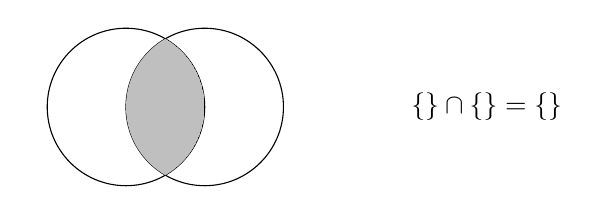
\begin{tikzpicture}[
	baseline=(current bounding box.north),
	set/.style = {
		circle,
		draw,
		minimum size = 2cm
	}
]
\node[set, label={180:\SM}] (M1) at (0,0) {};
\node[set, label={  0:\SM}] (M2) at (1,0) {};
\begin{scope}
	\clip (0,0) circle(1cm);
	\clip (1,0) circle(1cm);
	\fill[lightgray](0,0) circle(1cm);
\end{scope}
\node at (.5,0) {\SM};
\node[anchor=west,align=left] at (3.5,0) {$\{\SM\} \cap \{\SM\} = \{\SM\}$};
\end{tikzpicture}\medskip

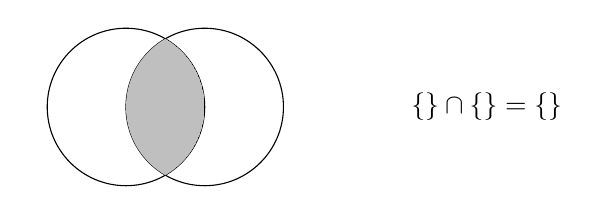
\begin{tikzpicture}[
	baseline=(current bounding box.north),
	set/.style = {
		circle,
		draw,
		minimum size = 2cm
	}
]
\node[set, label={180:\SF}] (F1) at (0,0) {};
\node[set, label={  0:\SF}] (F2) at (1,0) {};
\begin{scope}
	\clip (0,0) circle(1cm);
	\clip (1,0) circle(1cm);
	\fill[lightgray](0,0) circle(1cm);
\end{scope}
\node at (.5,0) {\SF};
\node[anchor=west,align=left] at (3.5,0) {$\{\SF\} \cap \{\SF\} = \{\SF\}$};
\end{tikzpicture}\medskip

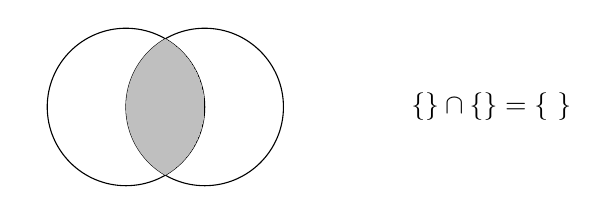
\begin{tikzpicture}[
	baseline=(current bounding box.north),
	set/.style = {
		circle,
		draw,
		minimum size = 2cm
	}
]
\node[set, label={180:\SM}] (M) at (0,0) {};
\node[set, label={  0:\SF}] (F) at (1,0) {};
\begin{scope}
	\clip (0,0) circle(1cm);
	\clip (1,0) circle(1cm);
	\fill[lightgray](0,0) circle(1cm);
\end{scope}
\node at (.5,0) {};
\node[anchor=west,align=left] at (3.5,0) {$\{\SM\} \cap \{\SF\} = \{\ \}$};
\end{tikzpicture}
\caption{Kombination der Sexus-Merkmale belebter Controller}
\label{fig:sexintersect}
\end{figure}

Die Menge an Belegen für den direkten Bezug zwischen Controller und Target ist
sowohl im \CAO{} als auch in der \KC{} sehr klein
(vgl.~\sectref{subsubsec:perscombsgnp}, \sectref{subsubsec:conomctrlpers}). Ein Beispiel für
die Kombination zweier weiblicher Controller mit direktem Bezug zum Target kann
im gesammelten Belegmaterial nicht gefunden werden.%
%
	\footnote{Kursorische Suchen im \CAO{} sowie im \REM{} nach kombinierten
	belebten Feminina, die direkt durch eine adjektivisch flektierende Wortart
	modifiziert werden, waren ergebnislos.}
%
Das zweite Diagramm in \figref{fig:sexintersect} ist daher eine begründete
Annahme, die sich auf Belege mit indirektem Bezug zwischen Controller und
Target stützt (siehe~\sectref{subsec:beid2p2coordrefl}). Das Beispiel in
\REF{ex:dietwill3} zeigt die Kombi\-nation zweier männlicher Personen; ein
Beispiel für die Kombination einer männlichen und einer weiblichen Person wurde
bereits in \REF{ex:gendres2} gegeben.

\begin{exe}
\ex\label{ex:dietwill3}
		\gll Willehalm vnd Dietreich. \\
			Willehalm[\textsc{nom.sg.\MascM}] und Dietrich[\textsc{nom.sg.\MascM}] \\
	\sn \gll wurden baíde da erſlagen. \\
			wurden beide-\textsc{nom.pl.\MascM.st} da erschlagen \\
		\trans `Willehalm und Dietrich wurden beide dort erschlagen.'
			(%
				C1:~83vb,36--37; vgl.
				K:~95vb,12--13%
			)
\end{exe}

\citet[576]{wechsler2009} und \citet[182]{wechslerzlatic2003} folgend lässt
sich die Situation auch für das Mittelhochdeutsche\il{Mittelhochdeutsch} so
erklären, dass zwei Typen von Genera unterschieden werden können: einerseits
Genera mit semantischen Korrelaten wie das Maskulinum und das Femininum und
andererseits Genera ohne semantische Korrelate wie das Neutrum.

\subsubsection{Unbelebte kombinierte Controller}
\label{subsubsec:x+x_dir_inan}

Der einzige Beleg im gesammelten Material für den direkten Bezug des Targets
auf zwei unbelebte Controller ist der in \REF{ex:hofzehntbeidiu} zitierte, der
mit \lit{hof} `Hof' und \lit{zehenden} `Zehnten' zwei Maskulina enthält. Diese
werden durch pronominal verwendetes \lit{beidev} aufgenommen, der Form nach ein
Neutrum. Dasselbe Muster zeigt sich beim indirekten Bezug zwischen Controllern
und Target noch weitere vier Male im \CAO{}. Die Frage ist, inwiefern dies
Regel oder Ausnahme darstellt. In regelmäßigen Fällen ist zu erwarten, dass
zwei maskulin-unbelebte Controller ein ebenfalls maskulines Target produzieren.

\begin{exe}
\ex\label{ex:hofzehntbeidiu}
	% Text auskommentiert, weil sonst Hurenkind resultiert :(
	\gll minen hof \textelp{} verkaufft han mit dem
			zehenden \textelp{}, beidev vnuerſchaidenlichen
			% fvͤr reht aigen
			\\
			meinen Hof[\textsc{acc.sg.\MascI}] {} verkauft habe mit dem
			Zehnt-\textsc{dat.sg.\MascI} {} beide-\textsc{acc.pl.\NeutI.st}
			gleichermaßen
			% für rechtmäßig Eigentum
			\\
	\trans `meinen Hof verkauft habe mit dem Zehnten \textelp{}, beide
		gleichermaßen%
		% zum rechtmäßigen Eigentum
		'
		\parencites(Nr.~N~241, Augsburg, 1283)[195,37--39]{cao5}
\end{exe}

Die Resolutionsform von Inanimata wird gemäß dem Modell von
\citet{wechsler2009} durch die Schnittmenge zwischen den grammatischen Genera
der Konjunkte und deren Schnittmenge mit der Menge der formalen Korrelate der
semantischen Geschlechter ($\SM \sim \textsc{m}$; $\SF \sim \textsc{f}$)
gebildet. Da das Neutrum die Resolutionsform darstellt, ist es mit $\{\ \}$
definiert
\autocites[vgl.][576--578]{wechsler2009}[184--186]{wechslerzlatic2003}. Damit
ergibt sich für das Mittelhochdeutsche\il{Mittelhochdeutsch} ein ähnliches
System wie im Färöischen\il{Färöisch} oder im Isländischen\il{Isländisch}
\autocites(vgl.~\figref{fig:iclgr})[225--226]{thrainsson2004}%
{wechsler2009}. Anders als das Mittelhochdeutsche\il{Mittelhochdeutsch}
besitzen diese im Nom.~Pl. (Isländisch\il{Isländisch} auch im Akk.~Pl.) der
starken Adjektivdeklination unterschiedliche Endungen für die einzelnen Genera,
siehe \tabref{tab:faerislmhdadj}.
% %
% 	\footnote{Für das Färöische\il{Färöisch} bzw.\ das
% 		Isländische\il{Isländisch} geben \citet[100--101]{thrainsson2004} und
% 		\citet[84--90]{kress1982} an:
% 		\fw{-ir}/\fw{-ar}/-Ø (Nom.~Pl.~M./F./N.) bzw.\ \fw{-a(r)}/\fw{-ar}/-Ø
% 		(Akk.~Pl.~M./F./N.). Dem gegenüber steht mhd.-obd.
% 		\fw{-e}/\fw{-e}/\fw{-iu} (Nom./Akk.~Pl.~M./F./N.;
% 		\cite[182--183]{ksw2}); siehe auch \tabref{tab:faerislmhdadj}.%
% 	}

\begin{figure}
	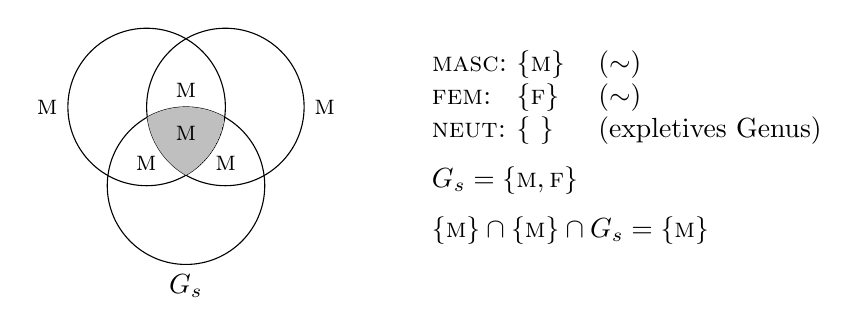
\begin{tikzpicture}[
		baseline=(current bounding box.north),
		set/.style = {
			circle,
			draw,
			minimum size = 2cm
		}
	]

	\node[set, label={180:\textsc{m}}]    (M1) at (0.0,+0.5) {};
	\node[set, label={  0:\textsc{m}}]    (M2) at (1.0,+0.5) {};
	\node[set, label={270:$G_s$}] (M3) at (0.5,-0.5) {};

	\begin{scope}
		\clip (0.0,+0.5) circle(1cm);
		\clip (1.0,+0.5) circle(1cm);
		\clip (0.5,-0.5) circle(1cm);
		\fill[lightgray](0.0,+0.5) circle(1cm);
	\end{scope}

	\node at (barycentric cs:M1=1,M2=1) [above]       {\textsc{m}};
	\node at (barycentric cs:M1=1,M3=1) [below left]  {\textsc{m}};
	\node at (barycentric cs:M2=1,M3=1) [below right] {\textsc{m}};
	\node at (barycentric cs:M1=1,M2=1,M3=1) {\textsc{m}};

	\node[anchor=west,align=left] at (3.5,0) {
		\begin{tabular}[b]{@{} >{\scshape}l @{~} l l @{}}
			masc: & $\{\textsc{m}\}$ & ($\sim \SM$) \\
			fem:  & $\{\textsc{f}\}$ & ($\sim \SF$) \\
			neut: & $\{\ \}$  & (expletives Genus) \\
		\end{tabular}\\[.5\baselineskip]

		$G_s = \{\textsc{m}, \textsc{f}\}$\\[.5\baselineskip]

		$\{\textsc{m}\} \cap \{\textsc{m}\} \cap G_s = \{\textsc{m}\}$
	};
	\end{tikzpicture}
\caption%
	{Kombination unbelebter Maskulina im Isländischen\il{Isländisch} nach
	\citet[578]{wechsler2009} und \citet[186]{wechslerzlatic2003}}
\label{fig:iclgr}
\end{figure}

Aus den Regeln in \figref{fig:iclgr} ergibt sich das abgebildete Schema,
das beim Bezug von \norm{bėide} auf zwei Maskulina eintritt. In den zwei
regelmäßigen Fällen im Belegmaterial \REF{ex:m+m_inan_e} unterscheiden die
betreffenden Urkunden in der Grafie deutlich zwischen den Typen \norm{-e} und
\norm{-iu}. Der regelmäßige Fall mit \norm{-e} ist im \CAO{} zweimal belegt und
damit über\-raschender\-weise weniger häufig als die fünf Fälle mit neutraler
Kongruenz wie in \REF{ex:hofzehntbeidiu}, die sich mit dem hier vorgestellten
theoretischen Ansatz nicht erklären lassen.

\begin{exe}
\ex \label{ex:m+m_inan_e}
	\begin{xlist}
	\ex \label{ex:m+m_inan_e_1}
		\gll vn̄ ain zehent in der pleſwicz · vn̄ ze Belen ain
				zehent die paid von dē patriarch ze
				lehent ſint \\
			und ein Zehnt[\textsc{acc.sg.\MascI}] in der Pleschivetz {} und zu
				Wöllan ein Zehnt[\textsc{acc.sg.\MascI}]
				\textsc{rel.nom.pl.\MascI} beide[\textsc{nom.pl.\MascI}] von
				dem Patriarch zu Lehen sind \\
		\trans `und einen Zehnten in Plešivec und in Velenje einen Zehnten, die
			beide vom Patriarchen zum Lehen sind'
			\parencites%
				(Nr.~2401, Haimburg, Bz.~Völkermarkt, 1296)
				[487,8--9]{cao3}[vgl.][502]{caor}

	\ex \label{ex:m+m_inan_e_2}
		\gll einen Weingarten \textelp{} Vnd einen Chrvͦtgarten
				\textelp{} · die geltent beide ſechſthalben
				ſchillinch \textelp{} \\
			einen Weingarten[\textsc{acc.sg.\MascI}] {} und einen
				Gemüsegarten[\textsc{acc.sg.\MascI}] {} {}
				\textsc{dem.nom.pl.\MascI} gelten
				beide-\textsc{nom.pl.\MascI.st} sechsthalben Schilling {} \\
		\trans `einen Weingarten \textelp{} und einen Gemüsegarten \textelp{},
			die bringen beide fünfeinhalb Schillinge \textelp{} ein.'
			\parencites(Nr.~2396, Regensburg, 1296)[484,28--30]{cao3}
	\end{xlist}
\end{exe}

\subsection{Indirekter Bezug zwischen Controller und Target}
\label{subsec:beid2p2coordrefl}

Wie bereits festgestellt, sind Kontexte, in denen das Target \norm{bėide} von
einem Pronomen abhängt, wesentlich häufiger als der direkte Bezug auf zwei
nominale Controller. Dabei hat das Target nur eine indirekte Verbindung zu
seinen nominalen \q{Erstcontrollern}. Im ausgewerteten Material sind die
Kombinationen von referenzierten Personenmerkmalen in diesem Kontext
vielfältiger als beim direkten Bezug, doch zeigen sich die gleichen Muster. Die
Untersuchung der Distanz zwischen Controller und Target (siehe dazu
\sectref{sec:caotargdist}, \sectref{sec:kctargdist}) hat ergeben, dass die Targets in diesen
Fällen sehr häufig in Kontaktstellung (\ref{ex:pronindir_1}) und seltener in
Distanzstellung (\ref{ex:pronindir_2}) zu ihren direkten Controllern stehen;
dasselbe beobachten auch \citet[624]{ksw2}. Mitunter lässt sich die
syntaktische Domäne nicht eindeutig feststellen, da manchmal beide Lesarten --
gefloatet und nicht-gefloatet, kollektiv und distributiv -- auch in
Kontaktstellung möglich sind, insbesondere, wenn \norm{si bėide} wie in
\REF{ex:pronindir_1} das Objekt darstellt (vgl.~\sectref{sec:floatquant}).

\begin{exe}
\ex \label{ex:pronindir}
	\begin{xlist}
	\ex \label{ex:pronindir_1}
		\gll vn̄ het er ir {die ſelben} Matta vfgegeben lidig vn̄ lere /
			vn̄ het ſi beide von ir enphangen \\
		und hat er ihr dieselben Wiese[\textsc{acc.pl.\FemI}] aufgegeben ledig
			und leer {} und hat \textsc{3pl\subI.acc}
			beide-\textsc{acc.pl.m+f\subI.st} von ihr empfangen \\
		\trans `außerdem hat er dieselben Wiesen frei und leer an sie
			ausgehändigt und hat sie beide von ihr \textins{als Lehen zurück'%
			empfangen}
			\parencites(Nr.~2733, Freiburg i.\,Br., 1297)[105,23--24]{cao4}

	\ex \label{ex:pronindir_2}
		\gll die herren chomen wider dô. \\
			die Herren[\textsc{nom.pl.\MascM}] kamen wieder dahin \\
			\textelp{}
	\sn \gll si frævten ſich baide da. \\
			\textsc{3pl\subM.nom} freuten sich beide-\textsc{nom.pl.\MascM.st}
			da \\
		\trans `Die Herren kamen wieder dahin \textelp{}. Sie freuten sich da
			beide.'
			(%
				C1:~11rb,7--10; vgl.
				K:~11vb,12--15;
				\KC:~V.~2055--2058;
				\cite[119]{schroeder1895}%
			)
	\end{xlist}
\end{exe}

Wie in \sectref{subsubsec:beid2p2snglncao} und \ref{subsubsec:beid2p2snglnkc}
zum indirekten Bezug von \norm{bėide} auf einzelne Plural-Erstcontroller
gezeigt, besteht in Fällen wie in \REF{ex:pronindir}, in denen das Target
indirekt von einem einzelnen Controller abhängt, keine Variation in der Flexion
zwischen \norm{bėide} und \norm{bėidiu} bei ansonsten gleichen
Personenmerkmalen. Die Targets flektieren stattdessen extrem regelmäßig
entsprechend dem Genus (\textsc{gend}) ihres Erstcontrollers, das heißt also,
nach formalen Personenmerkmalen. Daher findet sich in
\REF{ex:f+f_kindesibeidiu} die Form
\lit{peidev} in Kongruenz mit \lit{chinde} `Kinder'.

\begin{exe}
\ex \label{ex:f+f_kindesibeidiu}
	\gll ſweſter Gerdrauden vnd ſweſter Diemvden
			% hern wernhereſ chinden
			\textelp{} vnd ſwenne der vorbenannten chinde einez ſtirbet
			\textelp{} Di weil ſi peidev lebent \\
		Schwester Gertraut[\textsc{dat.sg.\FemF}] und Schwester
			Diemut[\textsc{dat.sg.\FemF}]
			% Herrn Wernhers Kinder-\textsc{dat.pl.\NeutF}
			{} und so=wenn der vorbenannten
			Kind-\textsc{gen.pl.\NeutF} eines stirbt {} die Weile
			\textsc{3pl\subF.nom} beide-\textsc{nom.pl.\NeutF.st} leben \\
	\trans `Schwester Gertraut und Schwester Diemut
		% , Herrn Wernhers Kindern
		\textelp{} Und wenn eines der vorgenannten Kinder stirbt \textelp{}
		Während sie beide leben'
		\parencites(Nr.~2960, Engelthal, Kr.~Nürnberger Land, 1298)[240,31--38]{cao4}
\end{exe}

Interessant ist diese Stelle, weil \norm{bėide} das Personalpronomen \norm{si}
`sie' modifiziert, sodass aufgrund der Wahrscheinlichkeit für semantische
Kongruenz bei pronominaler Referenz auch eine Form vom Typ \norm{bėide}
anstelle von \norm{bėidiu} möglich wäre, wie in \sectref{sec:gendsex}
ausgeführt, zumal die \lit{chinde} `Kinder' im Kontext namentlich als weiblich
identifiziert werden. Dem Zusammenhang nach handelt es sich bei ihnen nicht
notwendigerweise altersmäßig um Kinder, sondern um Kinder im
verwandt\-schaft\-lichen und rechtlichen Sinn, insofern Gertraut und Diemut
auch im Jugend- oder Erwachsenen\-alter Kinder ihrer Eltern bleiben
(\cites(Nr.~2960)[240,31+35]{cao4};
\cites(Nr.~2719)[vgl.~auch][96,40--97,18]{cao4}; \cite[569, 619]{caor}).

Dass sich \norm{si bėidiu} direkt auf Gertraut und Diemut bezieht, ist
zumindest unter formalen Gesichtspunkten unwahrscheinlich. Die Passage lautet
im Ganzen:

\begin{quote}
	\lit{vnd ſwenne der vorbenanten chinde einez ſtirbet · ſo ſchol dev
vor benant gvͦlte dem andern werden di weil ez lebet · Di weil ſi peidev lebent
ſo ſchol ſi avch in peiden werden} \autocites(Nr.~2960)[240,37--39]{cao4}

`Und wenn eines der vorgenannten Kinder
stirbt, soll die vorgenannte Rente dem anderen zufallen, während es lebt.
Während sie beide leben, soll sie auch ihnen beiden zufallen.'
\end{quote}

\subsubsection{Belebte kombinierte Controller}

Aus den Tabellen \tabref{tab:caosimprefctrl} und \tabref{tab:kcsimprefctrl} zur
Flexion von \norm{bėide} beim indirekten Bezug auf zwei Erstcontroller wurde
deutlich, dass nach einem Pronomen wie \norm{wir} `wir', \norm{si} `sie' oder
\norm{di} `die (\textsc{rel.pl')} bei übereinstimmendem Geschlecht im \CAO{}
stets die Form \norm{bėide} steht, bei unterschiedlichem Geschlecht dagegen
Variation zwischen \norm{bėidiu} \REF{ex:m+f_si_beidiu} und \norm{bėide}
\REF{ex:m+f_si_beide} herrscht.

\begin{exe}
\ex \label{ex:m+f_si_beide_iu}
	\begin{xlist}
	\ex \label{ex:m+f_si_beidiu}
		\gll hern Perhtolden dem Meinchovær vnd ſiner hoͮſfrowen ver Magereten
				vnd den chinden div ſi beidiv {mit ein ander} habent \\
			Herrn Berthold-\textsc{dat.sg.\MascM} dem Meinchauer und seiner
				Ehefrau[\textsc{dat.sg.\FemF}] Frau Margarete und den Kindern
				die \textsc{3pl\subMF.nom} beide-\textsc{nom.pl.\NeutMF.st}
				miteinander haben \\
		\trans `Herrn Berthold dem Meinchauer und seiner Ehefrau, Frau
			Margarete, und den Kindern, die sie beide miteinander haben'
			\parencites(Nr.~937, Regensburg, 1287)[292,40--41]{cao2}

	\ex \label{ex:m+f_si_beide}
		\gll Her Ernſt · vnſer burger / vnd ver Gerdroͤvt ſein hovsvrowe / da
				ſi baide lebten \\
			Herr Ernst[\textsc{nom.sg.\MascM}] {} unser Bürger {} und Frau
				Gertrud[\textsc{nom.sg.\FemF}] sein Ehefrau {} als
				\textsc{3pl\subMF.nom} beide-\textsc{nom.pl.m+f\subMF.st}
				lebten \\
		\trans `Herr Ernst, unser Bürger, und Frau Gertrud, seine Ehefrau,
			als sie beide am Leben waren'
			\parencites(Nr.~1073, Wien, 1289)[374,40--41]{cao2}
	\end{xlist}
\end{exe}

Wie bei der Diskussion der \CAO{}-Belege geschildert
(\sectref{subsubsec:monoflexioncao}), ist selbst bei
% den wenigen Fällen von
\norm{sie bėidiu} in bairischen\il{Bairisch} und \norm{siu bėide}
in alemannischen\il{Alemannisch} Urkunden davon auszugehen, dass
die Pronomen \norm{sie} und \norm{siu} als Varianten von invariablem \norm{si}
zu werten sind \autocite[vgl.][394--396]{ksw2}. In der \KC{} gibt es zumindest
einen Beleg für \norm{bėidiu} bei kombiniertem männlichen Bezug
\REF{ex:papstkoenig5}; bei unterschiedlichem Geschlecht liegt
\norm{bėidiu} in drei von insgesamt vier Fällen vor.

\begin{exe}
% "/" eingefügt und Zeilenumbrüche entfernt wegen Umbruch
\ex\label{ex:papstkoenig5} % 224
	\gll Der papſt vnd der chv̂nich {/} \\
		der Papst[\textsc{nom.sg.\MascM}] und der König[\textsc{nom.sg.\MascM}]
		\\
	% \gll Si warn zegot biderb vnd frumic {/} \\
	% 	sie waren {zu=Gott} brav und tüchtig \\
	% \gll Zegot ſtuͦnt allr ir geſín {/} \\
	% 	{zu=Gott} stand aller ihr Sinnen \\
	\textelp{}
	\gll Beideu ſchatz vnd gewín {/} \\
		beide Schatz und Gewinn \\
	\gll Liezzen ſi beideu gelich \\
		ließen \textsc{3pl\subM.nom} beide-\textsc{nom.pl.\NeutM.st} gleich \\
	\trans `Der Papst und der König
		% , sie waren Gott gegenüber brav und tüchtig. Auf Gott war all ihr
		% Sinnen gerichtet.
		\textelp{}
		Sowohl Schatz als auch Gewinn war ihnen beiden gleich.'
		(%
			B1:~17vb,30--34; vgl. abweichend
			\KC:~V.~6110--6113;
			\cite[202]{schroeder1895}%
		)
\end{exe}

Den Analysen von \citet{wechsler2009} und \citet{wechslerzlatic2003} zufolge
ist in Sprachen mit Gender Resolution im direkten Bezug auf koordinierte Nomina
mit semantischer Kongruenz zu rechnen. Bezüglich dieses syntaktischen Kontexts
wurde dies in \sectref{subsec:beid2coord} anhand der wenigen verfügbaren Beispiele
bereits deutlich. Im vorliegenden Abschnitt liegt allerdings indirekter Bezug
des Targets \norm{bėide} auf zwei nominale Controller vor. Das Schema in
\figref{fig:beid2p2coordn} illustriert diesen syntaktischen Kontext.

\begin{figure}
\centering
	\begin{tikzpicture}[baseline=(1a_lb.base)]
		\node at (0,2)  (1a)    [gray]
	                            {A};
		\node           (1a_box)[draw,gray,rectangle,fit=(1a)] {};
		\node           (1a_lb) [above=.5ex of 1a_box, gray, mynodefont]
	                            {controller 1};

		\node at (0,0)  (1b)    [gray]
		                        {B};
		\node           (1b_box)[draw,gray,rectangle,fit=(1b)] {};
		\node           (1b_lb) [above=.5ex of 1b_box, gray, mynodefont]
	                            {controller 2};    

		\node at (3,1) (2)      {sie};
		\draw (2) node (2_box1) [
		                    draw,
		                    gray,
		                    minimum height=3em,
		                    minimum width=3em,
		                    xshift=-.5ex,
		                    yshift=+.5ex,
		                    rectangle
		                ] {};
		\draw (2) node (2_box2) [
		                    draw,
		                    minimum height=3em,
		                    minimum width=3em,
		                    xshift=+.5ex,
		                    yshift=-.5ex,
		                    rectangle
		                ] {};
		\node           (2_lb1) [above=.5ex of 2_box1, gray, mynodefont]
		                        {target};
		\node           (2_lb2) [below=.5ex of 2_box2, mynodefont]
		                        {controller};

		\node at (6,1)  (3)      {beide};
		\node           (3_box)  [draw,rectangle,fit=(3)] {};
		\node           (3_lb)   [above=.5ex of 3_box, mynodefont]
		                        {target};

		\draw [-latex,gray] (1a_box) to [out=east, in=west] (2_box1);
		\draw [-latex,gray] (1b_box) to [out=east, in=west] (2_box1);
		\draw [latex-]      (3_box)  to [yshift=1.5ex]      (2_box2);
	\end{tikzpicture}
\caption{\fw{Sie} als Target und Controller gleichzeitig}
\label{fig:beid2p2coordn}
\end{figure}

Das direkte Antezedens von \norm{bėide} ist ein einzelnes Pronomen, in der
Regel ein Personal- oder Relativpronomen. Insbesondere in diesem Kontext kann
Variation beobachtet werden, wie in \REF{ex:m+f_si_beide_iu} exemplarisch
dargestellt. Es ist anzunehmen, dass die beiden möglichen Kongruenzstrategien
-- formale und semantische -- miteinander konkurrieren.
\citet[583]{wechsler2009} und \citet[194]{wechslerzlatic2003} zufolge wird in 
Sprachen, die beide Strategien anwenden, die semantische Zuweisung von Genus
zwar gewöhnlich durch formale Gender Resolution blockiert, jedoch nicht immer
vollständig, sodass die beiden Strategien in Konkurrenz zueinander stehen.

Das Pronomen \norm{si} in \figref{fig:beid2p2coordn} definiert die grammatischen
Eigenschaften in \figref{fig:beid2p2coordn_morphlex1}: Es handelt sich um ein
Personalpronomen im Nominativ Plural. Darüber hinaus referenziert dieses
Pronomen eine Gruppe von dritten Personen mit divergierenden
Geschlechtsmerkmalen. Das Pronomen \norm{si} ist selbst formal
genusindifferent.

\begin{figure}
\begin{tabular}[t]{@{} l @{\hspace{2em}} c @{\hspace{2em}} l}
	\norm{si}
		&	D
		&	\begin{tabular}[t]{l l l}
				\ups{pred}				& =	& $pro$ \\
				\ups{prontype}			& =	& $pers$ \\
				\ups{concord}			& =	& ↓ \\
					\quad\downs{num}	& =	& \textsc{pl} \\
					\quad\downs{case}	& =	& \textsc{nom} \\
					\quad\downs{gend}	& = & Ø \\
				\ups{index}			& =	& ↓ \\
					\quad\downs{pers}	& =	& 3 \\
					\quad\downs{num}	& =	& \textsc{pl} \\
					\quad\downs{sex}	& =	& $\SM \cap \SF$ \\
			\end{tabular}
			\\
\end{tabular}
\caption{Morpholexikalische Definition von \norm{si} `sie (\textsc{pl})'}
\label{fig:beid2p2coordn_morphlex1}
\end{figure}

Das Target \norm{bėide} in \figref{fig:beid2p2coordn_morphlex2} kongruiert mit
seinem Controller in den formalen Merk\-malen (\textsc{concord}): Kasus (case),
Genus (\textsc{gend}) und Numerus (\textsc{num}). Darüber hinaus koindiziert
(\textsc{index}) es seinen Controller mit dessen Merkmalen Person
(\textsc{pers}), Numerus (\textsc{num}) und Geschlecht (\textsc{sex}). Formal
wird vom Pronomen \norm{si} aber kein Genus (\textsc{gend}) festgelegt, mit dem
sein Target kongruieren könnte.

Das im ausgewerteten Material hauptsächlich beobachtete Muster entspricht der
gängigen Annahme, dass Kongruenztargets semantische Kongruenz dort zeigen, wo
der Controller für formale Kongruenzmerkmale lexikalisch nicht spezifiziert ist
\autocite[vgl.][191]{bresnanetal2016},%
%
	\footnote{\foreignblockcquote{english}[191]{bresnanetal2016}{%
		\textins*{A}greement targets \textelp{} show semantic agreement
		\emph{when the controller is lexically unspecified for the grammatical
		agreement features}}. An der zitierten Stelle ist
		\textquote{grammatical} als \q{formal} in Bezug auf das
		\textsc{concord}-Merkmal zu verstehen.%
	}
%
Das semantische Sexusmerkmal wird also in Abwesenheit des formalen
Genusmerkmals verwendet, um Kongruenz zu ermöglichen
\figref{fig:beid2p2coordn_morphlex2}. Die Kombination von männlicher und
weiblicher Referenz wird daher am Target zu einem Neutrum aufgelöst.

\begin{figure}
\begin{tabular}[t]{@{} l @{\hspace{2em}} c @{\hspace{2em}} l}
	\norm{bėidiu}
		&	Q
		&	\begin{tabular}[t]{l l l}
				\ups{pred}				& =		& `beide' \\
				\ups{index}			& =		& ↓ \\
					\quad\downs{pers}	& =		& \textsc{3} \\
					\quad\downs{num}	& =		& \textsc{pl} \\
					\quad\downs{sex}	& =		& $\SM \cap \SF$
						\tikzmark{b2p2cml1_sex}\\
				\ups{gf~concord}		& =		& ↓ \\
					\quad\downs{case}	& \req	& \textsc{nom} \\
					\quad\downs{num}	& \req	& \textsc{pl} \\
			\end{tabular}
	\\
\end{tabular}
\begin{tikzpicture}[remember picture, overlay]
	\draw [-latex]
		([yshift=1ex]{pic cs:b2p2cml1_sex})
		-- ++(east:1.5em) node[anchor=west] {\textsc{n} (\norm{-iu})};
\end{tikzpicture}
\caption{Morpholexikalische Definition von \norm{bėidiu} `beide' als semantische Resolutionsform}
\label{fig:beid2p2coordn_morphlex2}
\end{figure}

Um die trotz allem vorkommende Form \norm{bėide} zu erklären, wäre denkbar,
dass die Information des Sexusmerkmals formal interpretiert wird
\figref{fig:beid2p2coordn_morphlex4}: Ein Flexiv, das Maskulina und Feminina
gleichermaßen bezeichnet, ist mit \norm{-e} vorhanden. Da das Pronomen kein
Genusmerkmal definiert, läge auch damit keine Verletzung von
morphosyntaktischen Beschränkungen vor.

\begin{figure}
\begin{tabular}[t]{@{} l @{\hspace{2em}} c @{\hspace{2em}} l}
	\norm{bėide}
		&	Q
		&	\begin{tabular}[t]{l l l}
				\ups{pred}				& =		& `beide' \\
				\ups{index}			& =		& ↓ \\
					\quad\downs{pers}	& =		& \textsc{3} \\
					\quad\downs{num}	& =		& \textsc{pl} \\
					\quad\downs{sex}	& =		& $\SM \cap \SF$
						\tikzmark{b2p2cml2_sex}\\
				\ups{gf~concord}		& =		& ↓ \\
					\quad\downs{case}	& \req	& \textsc{nom} \\
					\quad\downs{gend}	& \req	& \gr{$\textsc{m} \lor \textsc{f}$}
						\tikzmark{b2p2cml2_gend}\\
					\quad\downs{num}	& \req	& \textsc{pl} \\
			\end{tabular}
	\\
\end{tabular}
\begin{tikzpicture}[remember picture, overlay]
	\draw [-latex, rounded corners=1ex]
		([yshift=.5ex]{pic cs:b2p2cml2_sex})
		-- ++(east:1em) |-
		([yshift=1ex]{pic cs:b2p2cml2_gend});
	\draw [-latex]
		([yshift=0ex]{pic cs:b2p2cml2_gend})
		-- ++(east:1.5em) node[anchor=west] {\textsc{m+f} (\norm{-e})};
\end{tikzpicture}
\caption{Morpholexikalische Definition von \norm{bėide} `beide' als semantisch basierte, formal flektierte Resolutionsform}
\label{fig:beid2p2coordn_morphlex4}
\end{figure}

Insofern angenommen werden kann, dass \norm{si bėide} bei Kontaktstellung eine
Phrase bildet, unterscheiden sich die betreffenden Schreiberinnen und Schreiber
der ausgewerteten Quellen vermutlich also in der Präferenz der anzuwendenden
Regel, das heißt, ob sie in Zweifelsfällen semantische Kongruenz oder formale
Kongruenz basierend auf semantischen Informationen anwenden. Im Belegmaterial
jedenfalls wird die \norm{iu}-Form stark bevorzugt, sehr regelmäßig sogar in
dem anderen syntaktischen Kontext mit eindeutiger Distanzstellung von `beide',
wie in \REF{ex:m+f_si_beidiu_float} illustriert (vgl.~auch
\tabref{tab:caoanadist}, \tabref{tab:kcanadist} zur Wortdistanz zwischen \norm{bėide} und
einem pronominalen Controller).

\begin{exe}
\ex \label{ex:m+f_si_beidiu_float}
	\gll vnd ſol {der ſelbe} vlrich / oder fraw Margret \textelp{}
			ſi leben peidev ſamte / oder ir æintwederez \\
		und soll derselbe Ulrich[\textsc{nom.sg.\MascM}] {} oder Frau
			Margarete[\textsc{nom.sg.\FemF}] {} \textsc{3pl\subMF.nom} leben
			beide-\textsc{nom.pl.\NeutMF.st} zusammen {} oder ihr
			entweder-\textsc{nom.sg.\NeutMF.st} \\
	\trans `Außerdem soll derselbe Ulrich oder Frau Margarete \textelp{}
		wenn sie beide zusammen am leben sind oder einer von ihnen'
		\parencites(Nr.~3141~A, Brixen, 1298)[352,3--9]{cao4}
\end{exe}

Das Target \norm{bėidiu} in \REF{ex:m+f_si_beidiu_float} befindet sich
ungeachtet der semantischen Zusammengehörigkeit in diesem Fall nicht in
derselben NP wie sein Controller \lit{vlrich / oder fraw Margret} `Ulrich oder
Frau Margarete', daher spielt formale Kongruenz in diesem Kontext kaum eine
Rolle. Belege für gefloatetes \norm{bėide} in Bezug auf gemischtgeschlechtliche
Controller sind nur vereinzelt vorhanden, stattdessen überwiegt semantische
Kongruenz, inklusive der dabei operierenden Gender Resolution.

Bezüglich der Kongruenzhierarchie (vgl.~\sectref{sec:kongrhier}) stellt sich die
Frage, in welcher Kongruenzdomäne gefloatete Quantoren einzuordnen sind. Im
Modell von \citet{corbett1979} und \citet[84]{wechslerzlatic2003} tauchen sie
als solche nicht auf. Zumindest beim kombinierten belebten Bezug ist regelmäßig
die neutrale statt der maskulin-femininen Form zu beobachten, wahrscheinlich
aufgrund von Gender Resolution, was widerum auf Koindizierung hinweist. Geht
man mit \citet{spector2009} aufgrund semantischer Differenzen (die auch
\cite{pittner1995} beobachtet) davon aus, dass Kontakt- und Distanzstellung von
Quantoren nicht nur semantisch, sondern auch funktional zu unterscheiden sind
(vgl.~dazu in \sectref{phsec:hebrqf}), müsste ein Floating Quantifier mit
Subjektbezug in dem Schema in \figref{fig:theoagrdist} neben dem primären
Prädikat (zum Beispiel prädikative Adjektive) anzusiedeln sein, da auch dieses
in einem anderen Satzteil desselben Teilsatzes steht und semantisch ein
Attribut des Subjekts darstellt. Nach der gröberen Einteilung von
\citet[216]{corbett1979} sollte es neben dem Relativpronomen stehen, da es
außerhalb des Satzteils seines Controllers steht, doch auf denselben Satz
beschränkt bleibt, in jedem Fall jedoch vor dem Personalpronomen, dessen Domäne
über den Satz hinausgeht.%

\subsubsection{Unbelebte kombinierte Controller}

Beim indirekten Bezug auf kombinierte unbelebte Controller steht ebenfalls nur
Belegmaterial aus dem \CAO{} zur Verfügung. Wie bei der Auswertung zur
Kongruenz von \norm{bėide} im indirekten Bezug auf kombinierte nominale
Controller in \sectref{subsubsec:beid2p2coordncao} beobachtet, ist der häufigste
Fall in unbelebten Kontexten eine Form des Typs \norm{bėidiu} unabhängig vom
Genus der Controller, wobei die Kombination zweier unbelebter Feminina nicht
belegt ist. Daneben stehen die zwei Belege in \REF{ex:m+m_inan_e2}, die die
maskulin-feminine Form \norm{bėide} in Einklang mit maskulinen Controllern
enthalten. Auch die zahlreichen Belege für \norm{bėidiu} mit indirektem Bezug
auf zwei Neutra \REF{ex:insigel} sind unauffällig. Gegenbelege mit
\norm{bėide}, die einer Erklärung bedürften, liegen keine vor.

\begin{exe}
\ex \label{ex:m+m_inan_e2}
	\begin{xlist}
	\ex \label{ex:m+m_inan_e2_1}
		\gll vn̄ ain zehent in der pleſwicz · vn̄ ze Belen ain zehent die paid
				von dē patriarch ze lehent ſint \\
			und ein Zehnt[\textsc{acc.sg.\MascI}] in der Pleschivetz {} und zu
				Wöllan ein Zehnt[\textsc{acc.sg.\MascI}] \textsc{rel.nom.pl.\MascI}
				beide[\textsc{nom.pl.\MascI}] von dem Patriarch zu Lehen sind \\
		\trans `und einen Zehnten in Plešivec und in Velenje einen Zehnten, die
			beide vom Patriarchen zum Lehen sind'
			(%
			\cites%
				(Nr.~2401, Haimburg, Bz.~Völkermarkt, 1296)[487,8--9]{cao3};
				vgl.~\cite[502]{caor}%
			)

	\ex \label{ex:m+m_inan_e2_2}
		\gll einen Weingarten \textelp{} Vnd einen Chrvͦtgarten \textelp{} ·
				die geltent beide ſechſthalben ſchillinch \textelp{} \\
			einen Weingarten[\textsc{acc.sg.\MascI}] {} und einen
				Gemüsegarten[\textsc{acc.sg.\MascI}] {} {}
				\textsc{rel.nom.pl.\MascI} gelten
				beide-\textsc{nom.pl.\MascI.st} sechsthalben Schilling {} \\
		\trans `einen Weingarten \textelp{} und einen Gemüsegarten \textelp{},
			die beide fünfeinhalb Schillinge \textelp{} einbringen.'
			\parencites(Nr.~2396, Regensburg, 1296)[484,28--30]{cao3}
	\end{xlist}
\end{exe}

Wie aussagekräftig sind die Belege in \REF{ex:m+m_inan_e2} angesichts des
Umstands, dass der erwartete Regelfall zahlenmäßig die Ausnahme darstellt? Die
Urkunde zu \REF{ex:m+m_inan_e2_1} enthält neben \lit{mit allev dew} `mit all
dem' und \lit{auf alle deu} `auf alle die'
\autocites(Nr.~2401)[487,11+17]{cao3} als Rest des Instrumentals
\autocite[vgl.][618]{ksw2} nur \norm{die} als Relativpronomen, dafür aber stets
in formalem Einklang mit seinem Controller. Anzumerken ist, dass das
Relativpronomen und \norm{bėide} in unterschiedlichen Phrasen stehen, also
trotz oberflächlicher Kontaktstellung in der C-Struktur Distanzstellung
vorliegt. Da das Relativpronomen in \figref{fig:dibeidecstruct} die
Subjektposition einnimmt (hier die DP-Schwester von \xbar{C}) und das finite
Verb im Relativsatz in der rechten Satzklammer steht, bleibt die linke
Satzklammer (\xhead{C}) leer. In der linearen Abfolge der Wortformen steht
daher \norm{bėide} direkt hinter \norm{die}, auch wenn \norm{die} und
\norm{bėide} zusammen keine Phrase bilden.

\begin{figure}
\begin{forest} shorter edges, align text,
[CP
	[DP
		[\xhead{D}
			[\textit{die}]
		]
	]
	[\xbar{C}
		[\xhead{C}
			[Ø]
		]
		[VP
			[QP
				[\xhead{Q}
					[\textit{beide}]
				]
			]
			[\xbar{V}
				[\dots]
			]
		]
	]
]
\end{forest}
\caption{Konstituenz des Satzfragments \fw{\dots, die beide \dots}}
\label{fig:dibeidecstruct}
\end{figure}

Die in \REF{ex:m+m_inan_e2_2} zitierte Urkunde unterscheidet zumindest beim
definiten Artikel regelmäßig zwischen \norm{die} und \norm{diu}. In beiden
Urkunden spricht nichts ausdrücklich gegen die Annahme, dass \norm{die} die
maskulin-feminine Form des Relativpronomens darstellt. Das von diesem Pronomen
abhängige Target \norm{bėid(e)} kann problemlos mit dem Genusmerkmal des
jeweiligen pronominalen Controllers kongruieren, da sich dieser auf zwei
Maskulina bezieht.

Wie bei den Belegen mit direktem Bezug kann das Auftreten von neutralem
\norm{bėidiu} bei verschiedenem Geschlecht der Erstcontroller mit einer
Mengenoperation analog zu der in \figref{fig:iclgr} erklärt werden; illustriert
wird dies in \figref{fig:iclgr2_1}--\ref{fig:iclgr2_3}. Maskulin und Feminin
haben zwar jeweils eine Schnittmenge mit der Menge der semantisch gekoppelten
Genera ($G_s$), allerdings nicht miteinander. In \figref{fig:iclgr2_1} zu
\REF{ex:iclgr2_1} resultiert daher eine leere Menge $\{\ \}$ die dem Neutrum
als Resolutionsgenus entspricht. In den anderen beiden Fällen mit Neutrum,
\REF{ex:iclgr2_2} und \REF{ex:iclgr2_3} mit \figref{fig:iclgr2_2} und
\ref{fig:iclgr2_3}, kommt es nur jeweils beim Maskulinum und beim Femininum zu
einer Schnittmenge mit $G_s$, aber nirgends sonst, sodass auch dort nur das
Neutrum als Lösung bleibt.

\begin{exe}
\ex \label{ex:iclgr2}
\begin{xlist}
	\ex \label{ex:iclgr2_1}
		\gll % vnd verzeih mich / \textelp{}
			dez Cehenten vnd der huͦb / dev paidev {vor benemt} ſint \\
			% und verzichte mich {} {}
			des Zehnten[\textsc{gen.sg.\MascI}] und der
				Hube[\textsc{gen.sg.\FemI}] {} \textsc{rel.nom.pl.\NeutI}
				beide-\textsc{nom.pl.\NeutI.st} vorgenannt sind \\
			\trans `\textins{und verzichte \dots} auf den Zehnten und die Hube,
				die beide vorgenannt sind'
				\parencites(Nr.~3261, Regensburg, 1299)[424,38--39]{cao4}

	\begin{figure}
	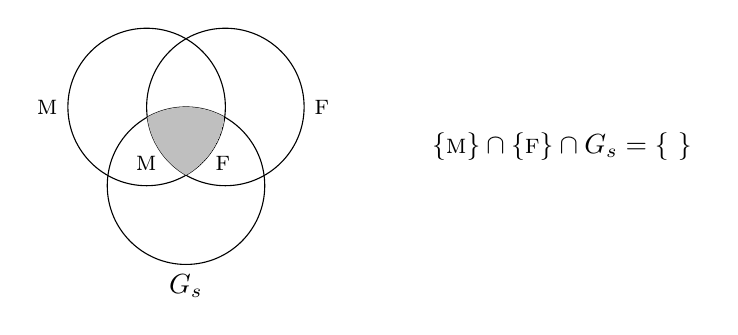
\begin{tikzpicture}[
		baseline=(current bounding box.north),
			set/.style = {
				circle,
				draw,
				minimum size = 2cm
			}
		]
		\node[set, label={180:\textsc{m}}]    (M)  at (0.0,+0.5) {};
		\node[set, label={  0:\textsc{f}}]    (F)  at (1.0,+0.5) {};
		\node[set, label={270:$G_s$}] (MF) at (0.5,-0.5) {};
		\begin{scope}
			\clip (0.0,+0.5) circle(1cm);
			\clip (1.0,+0.5) circle(1cm);
			\clip (0.5,-0.5) circle(1cm);
			\fill[lightgray](0.0,+0.5) circle(1cm);
		\end{scope}
		\node at (barycentric cs:M=1,MF=1) [below left]  {\textsc{m}};
		\node at (barycentric cs:F=1,MF=1) [below right] {\textsc{f}};
		\node at (barycentric cs:M=1,F=1,MF=1) {};
		\node[anchor=west,align=left] at (3.5,0) {
			$\{\textsc{m}\} \cap \{\textsc{f}\} \cap G_s = \{\ \}$
		};
	\end{tikzpicture}
	\caption{Kombination von unbelebtem Maskulinum und Femininum}
	\label{fig:iclgr2_1}
	\end{figure}

	\ex \label{ex:iclgr2_2}
		\gll einen Hof / vnd ein Lehen - da pei / vnd ſind paidev æigen \\
			einen Hof[\textsc{acc.sg.\MascI}] {} und ein
				Lehen[\textsc{acc.sg.\NeutI}] {} da bei {} \textsc{rel}
				sein[\textsc{3pl\subM.ind.prs}] beide-\textsc{nom.pl.\NeutI.st}
				Eigentum \\
			\trans `einen Hof und ein Lehen in der Nähe, die beide Eigentum
				sind'
				\parencites(Nr.~1923, Steyr, 1294)[194,36--37]{cao3}

	\begin{figure}
	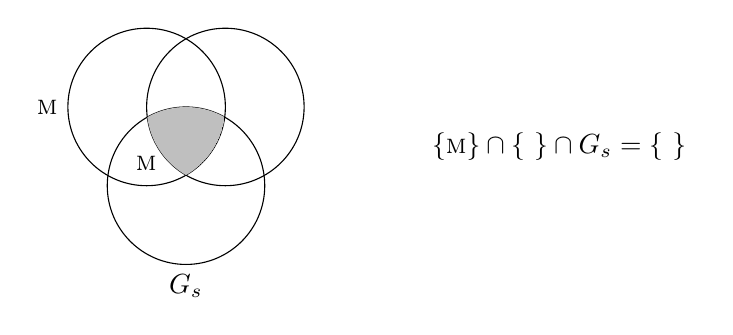
\begin{tikzpicture}[
			baseline=(current bounding box.north),
			set/.style = {
				circle,
				draw,
				minimum size = 2cm
			}
		]
		\node[set, label={180:\textsc{m}}]    (M)  at (0.0,+0.5) {};
		\node[set, label={  0:}]      (N)  at (1.0,+0.5) {};
		\node[set, label={270:$G_s$}] (MF) at (0.5,-0.5) {};
		\begin{scope}
			\clip (0.0,+0.5) circle(1cm);
			\clip (1.0,+0.5) circle(1cm);
			\clip (0.5,-0.5) circle(1cm);
			\fill[lightgray](0.0,+0.5) circle(1cm);
		\end{scope}
		\node at (barycentric cs:M=1,MF=1) [below left] {\textsc{m}};
		\node at (barycentric cs:M=1,N=1,MF=1) {};
		\node[anchor=west,align=left] at (3.5,0) {
			$\{\textsc{m}\} \cap \{\ \} \cap G_s = \{\ \}$
		};
	\end{tikzpicture}
	\caption{Kombination von unbelebtem Maskulinum und Neutrum}
	\label{fig:iclgr2_2}
	\end{figure}

	\ex \label{ex:iclgr2_3}
		\gll daz ich auz minem hauz vnd auz miner hofſtat div bediv min recht
				eigen ſint \textelp{} \\
			dass ich aus meinem Haus[\textsc{dat.sg.\NeutI}] und aus meiner
				Grundstück[\textsc{dat.sg.\FemI}] \textsc{rel.nom.pl.\NeutI}
				beide-\textsc{nom.pl.\NeutI.st} mein rehtmäßig Eigentum sind {}
				\\
			\trans `dass ich aus meinem Haus und aus meinem Grundstück, die
				beide mein rechtmäßiges Eigentum sind \textelp{}'
				\parencites(Nr.~1282, Ulm und Kl.~Raitenhaslach, Kr.~Altötting, 1282)[526,37--38]{cao2}

		\begin{figure}
		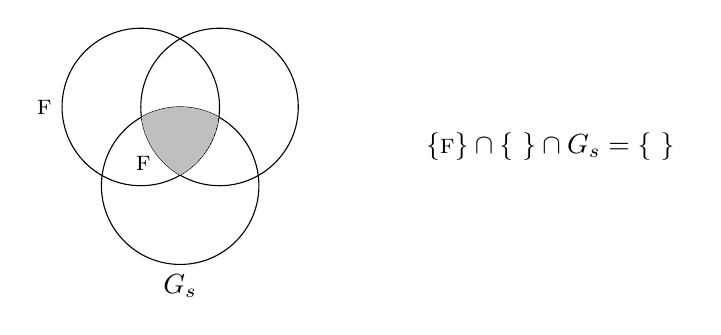
\begin{tikzpicture}[
				baseline=(current bounding box.north),
				set/.style = {
					circle,
					draw,
					minimum size = 2cm
				}
			]
			\node[set, label={180:\textsc{f}}]    (F)  at (0.0,+0.5) {};
			\node[set, label={  0:}]      (N)  at (1.0,+0.5) {};
			\node[set, label={270:$G_s$}] (MF) at (0.5,-0.5) {};
			\begin{scope}
				\clip (0.0,+0.5) circle(1cm);
				\clip (1.0,+0.5) circle(1cm);
				\clip (0.5,-0.5) circle(1cm);
				\fill[lightgray](0.0,+0.5) circle(1cm);
			\end{scope}
			\node at (barycentric cs:F=1,MF=1) [below left] {\textsc{f}};
			\node at (barycentric cs:F=1,N=1,MF=1) {};
			\node[anchor=west,align=left] at (3.5,0) {
				$\{\textsc{f}\} \cap \{\ \} \cap G_s = \{\ \}$
			};
		\end{tikzpicture}
		\caption{Kombination von unbelebtem Femininum und Neutrum}
		\label{fig:iclgr2_3}
		\end{figure}
	\end{xlist}
\end{exe}

\subsection{Neutrum bei maskulinem und femininem Bezug}
\label{subsec:m+m_anim_beidiu}

Neben regelmäßigen Fällen, in denen die Kombination zweier Maskulina die Form
\norm{bėide} ergibt, zeigten sich sowohl mit Bezug auf belebte als auch auf
unbelebte maskuline (Erst-)Controller mehrere Vorkommen von neutralem
\norm{bėidiu}. Diese verteilen sich auf alle untersuchten Kontexte, wie
beispielhaft in \REF{ex:m+m_beidiu} gezeigt, mit Ausnahme der Abhängigkeit von
pronominalen Controllern mit belebter Referenz.

\begin{exe}
\ex \label{ex:m+m_beidiu}
	\begin{xlist}
	\ex \label{ex:m+m_beidiu_1}
		\gll Die rihtær ſprachen beideu {dar zuͦ} \\
			die Richter[\textsc{nom.pl.\MascM}] sprachen
			beide-\textsc{nom.pl.\NeutM.st} dazu \\
		\trans `Die Richter äußerten sich beide dazu'
			(%
				B1:~28ra,8; vgl.~abweichend
				\KC:~V.~10090;
				\cite[267]{schroeder1895}% 1140 mit Parallelstelle in H
			)

	\ex \label{ex:m+m_beidiu_3}
		\gll Diſ dingeſ gezuga ſint · Ruͦd · von der palma min Oͤhen · vͦlrich
				von Grvͤnenberch min Oͤhen bedu Jungherren \textelp{} \\
			Dies Verhandlung-\textsc{gen.sg.\NeutI} Zeugen sind {}
				\lit{Ruͦd}[\textsc{nom.sg.\MascM}] {} von der Palme mein Oheim
				{} Ulrich[\textsc{nom.sg.\MascM}] von Grünenberg mein Oheim
				beide-\textsc{nom.pl.\NeutM.st}
				Jungherren[\textsc{nom.pl.\MascM}] {} \\
		\trans `Zeugen dieser Verhandlung sind: \lit{Ruͦd} von der Palme,
			mein Onkel, Ulrich von Grünenberg, mein Onkel -- beide Junker --
			\textelp{}'
			\parencites(Nr.~2915, Kl.~St.~Urban, Kt.~Luzern, 1298)[213,33--35]{cao4}

	% \ex \label{ex:m+m_beidiu_5}
	% 	\gll vnſerne zehenden zeandeluingen vnde ainen Garten indem ſelben
	% 			dorfe \textelp{} div wier baidiv fvr reht aigen her
	% 			haigen~\textins{sic} braht \\
	% 		unseren Zehnt-\textsc{acc.sg.\MascI} zu=Andelfingen und einen
	% 			Garten-\textsc{acc.sg.\MascI} in.dem selben Dorf {}
	% 			\textsc{rel.acc.pl.\NeutI} wir beide-\textsc{acc.pl.\NeutI.st}
	% 			für rehtmäßig Eigentum her haben gebracht \\
	% 	\trans `unseren Zehnten in Andelfingen und einen Garten in
	% 		demselben Dorf \textelp{}, die wir beide zum rechtmäßigen Eigentum
	% 		\textins{dar}gebracht haben'
	% 		\parencites(Nrn.~1201~AB, Kl.~Heiligkreuztal, Kr.~Biberach, 1290)[472,10--14]{cao2}

	\ex \label{ex:m+m_beidiu_5}
		\gll vnſerne zehenden \textelp{} vnde ainen Garten \textelp{} div wier
				baidiv fvr reht aigen her haigen~\textins{sic} braht \\
			unseren Zehnt-\textsc{acc.sg.\MascI} {} und einen
				Garten-\textsc{acc.sg.\MascI} {} \textsc{rel.acc.pl.\NeutI} wir
				beide-\textsc{acc.pl.\NeutI.st} für rehtmäßig Eigentum her
				haben gebracht \\
		\trans `unseren Zehnten \textelp{} und einen Garten \textelp{}, die wir
			beide zum rechtmäßigen Eigentum \textins{dar}gebracht haben'
			\parencites(Nrn.~1201~AB, Kl.~Heiligkreuztal, Kr.~Biberach, 1290)[472,10--14]{cao2}

	\end{xlist}
\end{exe}

Der Beleg in \REF{ex:m+m_beidiu_1} enthält ein \norm{bėidiu}-Target, das sich
unmittelbar auf das Plural-Maskulinum \lit{rihtær} `Richter' bezieht, das
seinerseits männlich denotiert ist. Bei \REF{ex:m+m_beidiu_3} bezieht sich
\lit{bedu} entweder direkt auf die beiden Herren
\lit{Ruͦd}\textins{\norm{iger}/\norm{olf}?} und \lit{vͦlrich} oder auf
\lit{Jungherren} `Junker'. In jedem Fall ist die Kongruenzform von \norm{bėide}
anomal. Zuletzt bezieht sich die neutrale Form \lit{baidiv} in
\REF{ex:m+m_beidiu_5} dem Kontext nach am ehesten auf \lit{zehenden} `Zehnten'
und \lit{Garten} `Garten'. Da es sich bei den Ausstellern der Urkunde um die
drei Brüder \lit{wezel vn̄ hainrich wezel vnde Cvͦnrat de\textins{n} Bodemer}
\autocites(Nrn.~1201~AB)[472,6--7]{cao2} handelt, wird sich \lit{baidiv} nicht
auf \lit{wier} beziehen. Vielmehr wurde die Stelle so interpretiert, dass der
Zehnt und der Garten gemeinsam im Rahmen der Verkaufsverhandlung als
rechtmäßiges Eigentum dargebracht wurden.

Das theoretische Modell von \citet{wechsler2009} und \citet{wechslerzlatic2003}
vermag diese Ausnahmen nicht zu erklären. Die \tabref{tab:m+m_beidiu} zeigt die
Verteilung der Formen mit Bezug auf maskulin-männliche und maskulin-unbelebte
Controller auf die unterschiedlichen belegten syntaktischen Kontexte.
Hervorzuheben ist, dass insgesamt lediglich neun Belege in der gesamten
Stichprobe betroffen sind -- sechs im ausgewertete Material des \CAO{} und
weitere drei in der Stichprobe zur \KC{}. Es handelt sich hier also eher um
eine Randerscheinung.

\begin{table}[t]
\setlength{\tabcolsep}{5pt}
\caption{Form von \norm{bėide} in Bezug auf männliche bzw.\ maskuline
Controller}
\begin{tabular}{
	c c c
	r r
	c
	r r
	r
}
\lsptoprule

\mr{2}{*}[-.5ex]{Controller}
	& \mr{2}{*}[-.5ex]{Merkmal(e)}
	& \mr{2}{*}[-.5ex]{Float}
	& \mc{2}{c}{\CAO{}}
	& %
	& \mc{2}{c}{\KC{}}
	& \mr{2}{*}[-.5ex]{Summe}
	\\

\cmidrule{4-5}
\cmidrule{7-8}

%
	& %
	& %
	& \norm{bėid(e)}
	& \norm{bėidiu}
	& %
	& \norm{bėid(e)}
	& \norm{bėidiu}
	& %
	\\

\midrule

$N_i$
	& \MascM
	& $-$
	&  25 % CAO beide
	& % CAO beidiu
	& %
	&   3 % KC beide
	& % KC beidiu
	&  28 % Summe
	\\

%
	& %
	& $+$
	& % CAO beide
	& % CAO beidiu
	& %
	&   2 % KC beide
	&   2 % KC beidiu
	&   4 % Summe
	\\

\cmidrule{2-9}

%
	& \MascI
	& $-$
	&   8 % CAO beide
	& % CAO beidiu
	& %
	& % KC beide
	& % KC beidiu
	&   8 % Summe
	\\

\midrule

$N_i + N_j$
	& $\MascM+\MascM$
	& $-$
	& % CAO beide
	&   1 % CAO beidiu
	& %
	& % KC beide
	& % KC beidiu
	&   1 % Summe
	\\

%
	& %
	& $+$
	&   1 % CAO beide
	& % CAO beidiu
	& %
	&   2 % KC beide
	&   1 % KC beidiu
	&   4 % Summe
	\\

\cmidrule{2-9}

%
	& $\MascI+\MascI$
	& $+$
	& % CAO beide
	&   1 % CAO beidiu
	& %
	& % KC beide
	& % KC beidiu
	&   1 % Summe
	\\

\midrule

$PRO_i$
	& \MascM
	& $-$
	&   3 % CAO beide
	& % CAO beidiu
	& %
	& % KC beide
	& % KC beidiu
	&   3 % Summe
	\\

%
	& %
	& $+$
	& % CAO beide
	& % CAO beidiu
	& %
	&   7 % KC beide
	& % KC beidiu
	&   7 % Summe
	\\

\midrule

$PRO_{i + j}$
	& $\MascM+\MascM$
	& $-$
	&  15 % CAO beide
	& % CAO beidiu
	& %
	&   1 % KC beide
	& % KC beidiu
	&  16 % Summe
	\\

%
	& %
	& $+$
	&  10 % CAO beide
	& % CAO beidiu
	& %
	&  12 % KC beide
	& % KC beidiu
	&  22 % Summe
	\\

\cmidrule{2-9}

%
	& $\MascI+\MascI$
	& $-$
	& % CAO beide
	&   1 % CAO beidiu
	& %
	& % KC beide
	& % KC beidiu
	&   1 % Summe
	\\

%
	& %
	& $+$
	&   2 % CAO beide
	&   3 % CAO beidiu
	& %
	& % KC beide
	& % KC beidiu
	&   5 % Summe
	\\

\midrule

\mc{3}{l}{Summe}
	&  64 % CAO beide
	&   6 % CAO beidiu
	& %
	&  27 % KC beide
	&   3 % KC beidiu
	& 100 % Summe
	\\

\lspbottomrule	
\end{tabular}
\label{tab:m+m_beidiu}
\end{table}

\citet[581]{wechsler2009} und \citet[190]{wechslerzlatic2003} merken
hinsichtlich ähnlicher Fälle im
Bosnisch-\allowbreak{}Kroatisch-\allowbreak{}Mazedonisch-\allowbreak{}Serbischen
(\ili{BKMS}) an, dass \citet{corbett1983,corbett1991} basierend auf
Textbeispielen viele Ausnahmen zu seiner Resolutionsregel vermelde, insofern
das Maskulin-Plural-Default übermäßig auf solche Kontexte angewandt wird, die
allein aus femininen Konjunkten bestehen. Auf die Situation im
Mittelhochdeutschen\il{Mittelhochdeutsch} übertragen ist anzunehmen, dass das
Neutrum als Resolutionsgenus auf die anderen beiden Geschlechter übergreift. In
den hier ausgewerteten Quellen lässt sich dies für das Femininum aufgrund
fehlender Belege nicht nachvollziehen, wohl aber für das Maskulinum. Mit
Verweis auf \citet[302]{corbett1991} schreiben \citet[581]{wechsler2009} und
\citet[190]{wechslerzlatic2003} weiter, dass dieser bemerke, keine Beispiele
für maskuline Kongruenz mit femininen Nomina, die sich auf Personen beziehen,
gefunden zu haben. Sie schließen daraus, dass (zumindest im BKMS) mit Kongruenz
entgegen dem semantischen Geschlecht belebter Referenten nicht zu rechnen ist,
während die schwächere, abgeleitete Resolutionsregel für unbelebte Referenten
gelegentlich verletzt wird.

Aus \tabref{tab:m+m_beidiu} ergibt sich, dass \norm{bėidiu} mit männlichem Bezug
im \CAO{} nur in Kontexten mit kombinierter Referenz auftritt, sowohl bei
direktem als auch indirektem Bezug auf die Controller, sowohl in
Kontaktstellung als auch in Distanzstellung. Zwei Belegen mit belebt-männlicher
Referenz stehen vier mit unbelebt-maskuliner gegenüber. In der \KC{} dagegen
tritt \norm{bėidiu} nur beim direkten Bezug auf, dafür aber sowohl in Kontexten
mit kombinierter als auch einfacher Referenz, und nur in Distanzstellung.
Inanimata sind in der Stichprobe zur \KC{} nicht vertreten. Abgesehen davon,
dass für die \KC{} nur drei verwendbare Belege vorliegen gegenüber den sechs
Belegen beim \CAO{}, verhalten sich beide Datenserien konträr zueinander.

Dadurch, dass neutrales \norm{bėidiu} mit maskuliner Referenz hauptsächlich mit
unbelebten Controllern einhergeht, gilt zumindest für das \CAO{} eingeschränkt
die oben zitierte Schlussfolgerung, dass sich das Übergreifen des
Resolutionsgenus in solchen Kontexten bemerkbar mache, in denen die formale
Ausgleichsregel bei Inanimata eintritt (siehe \REF{ex:gendasshier}). Die zweite
Hälfte der These, dass dies nur bei unbelebten Targets der Fall sei, trifft auf
die Beleglage im \CAO{} nicht ganz zu, und gar nicht auf die \KC{}. Aus dem
synchronen System des Mittelhochdeutschen\il{Mittelhochdeutsch} um 1300 heraus
ist jedenfalls formal nicht nachvollziehbar, warum zwei Maskulina in manchen
Fällen kombiniert als Neutrum aufgenommen werden.

Unter einer geografischen Perspektive ist festzustellen, dass die \CAO{}-Belege
zum Neutrum mit Bezug auf Maskulina aus Augsburg, Freiburg i.\,Br., dem Kloster
Heiligkreuztal (Kr.~Biberach) und dem Kloster St.~Urban (Kt.~Luzern) stammen.
Diese Orte liegen alle im alemannisch-\il{Alemannisch} und
schwäbischsprachigen\il{Schwäbisch} Gebiet. Im Fall der \KC{} sind die
Handschriften K und B1 aus dem alemannischen\il{Alemannisch} beziehungsweise
aus dem mittelbairischen\il{Bairisch} Sprachraum betroffen. Damit stammen
insgesamt sieben Belege für dieses Phänomen aus dem West- und zwei aus dem
Ost\-ober\-deutschen\il{Bairisch}.

Während im untersuchten Material keine Kombination von zwei unbelebten Feminina
vorkommt (bezogen auf die Kombination von belebten Feminina steht immer
\norm{bėide}), liefert \citet[384]{paul2007} zur Illustration des Phänomens den
in \REF{ex:walther92_25-28_C_2} zitierten Beleg. Dort steht in Bezug auf die
Abstrakta \lit{liͤbe} `Liebe' und \lit{ſchoͤne} `Schönheit' das Demonstrativum
\lit{diſiu̍} `diese', das zumindest der Form nach als Neutrum erscheint
\autocite[485]{ksw2}. Das folgende \lit{beide} hat dagegen eine Form, die der
Annahme von femininer Kongruenz zumindest nicht entgegen steht. Mit dem hier
aufgestellten theoretischen Modell kann dieser Beleg nicht erklärt werden.

\begin{exe}
\ex\label{ex:walther92_25-28_C_2}
	\gll du̍ liͤbe ſtet der ſchoͤne bi~· \\
			die Liebe[\textsc{nom.sg.\FemI}] steht der
			Schönheit[\textsc{dat.sg.\FemI}] bei \\
\sn \gll bas danne geſteine dē golde tvͦt~· \\
		besser als Edelstein dem Gold tut \\
\sn \gll nv iehet wc danne beſſer ſi~· \\
		nun sprecht was daher besser sei \\
\sn \gll hant diſu̍ beide rehten mvͦt~· \\
		haben dies-\textsc{nom.pl.\NeutI.st} beide-\textsc{nom.pl.m+f\subI.st}
			gehörigen Gesinnung \\
	\trans `Die Liebe passt zur Schönheit besser als die Edelsteine zum
		Gold: Nun sprecht, was daher besser sei, wenn diese beide gehöriger
		Gesinnung sind.'
		(%
			\iai{Walther von der Vogelweide}: 92,25--28 nach
			Heidelberg, Universitätsbibl., Cod.~Pal.~germ.~848: 128rb,1--4;
			% [\cite[4957]{hsc}],
			vgl.~\cite[356--358]{bein2013}%
		)
	\\
\end{exe}

\citeauthor{ksw2} merken an, dass Formen vom Typ \norm{disiu} in
alemannischen\il{Alemannisch} Quellen
\blockcquote[485]{ksw2}{\textins{v}ereinzelt auch im Nom.Pl.Fem.} auftreten --
es wird angenommen, dass der Kodex Manesse im Raum Zürich um 1300 entstand
\autocite[4957]{hsc}. \Citet{deboor1976b} attestiert
alemannischen\il{Alemannisch} Urkundenschreibern
\blockcquote[27]{deboor1976b}{Anzeichen von Unsicherheit in der richtigen
Verwendung von \norm{disiu}}. Er vermutet, dass sie
\blockcquote[28]{deboor1976b}{\norm{disiu} \textins{schrieben}, wie sie es
gelernt hatten, wo in der mündlichen Verhandlung schon \norm{dise} gesprochen
wurde, und es passierte ihnen, daß sie \norm{disiu} schrieben, auch wo
\norm{dise} richtig war}. Festzuhalten ist, dass sich in
alemannischen\il{Alemannisch} Urkunden des späten 13.~Jahrhunderts
ein Schwanken zwischen \norm{dise} und \norm{disiu} beobachten lässt, das auch
den Beleg in \REF{ex:walther92_25-28_C_2} erklären könnte. Es lässt sich
annehmen, dass das ursprüngliche System der Pluralkongruenz im Genus durch die
Ausweitung der maskulin-femininen Form für Schreiberinnen und Schreiber aus dem
alemannischen\il{Alemannisch} Gebiet um 1300 nicht mehr klar
erkennbar war.

\subsection{Zusammenfassung}

Als Modell zur theoretischen Reflexion der ausgewerteten Belege aus dem
\CAO{} und der \KC{} wurde das in \citet{wechsler2009} und
\citet{wechslerzlatic2003} vorgestellte Modell zur Erklärung herangezogen.
Dieses basiert auf der LFG und fasst Gender Resolution als
Schnittmengenoperation auf. Die von \citet[578]{wechsler2009} und
\citet[186]{wechslerzlatic2003} für das moderne Isländische\il{Isländisch}
formulierten Regeln lassen sich auch auf den Großteil der gesammelten
mittelhochdeutschen\il{Mittelhochdeutsch} Belege anwenden.

Der Bezug von \norm{bėide} auf einzelne Substantive im Plural -- sowohl direkt
als auch indirekt -- bereitete keine Probleme. Die Belege zeigen bis auf wenige
Ausnahmen regelmäßig formale Kongruenz. Interessant, aber nicht durch die
gesammelten Belege zu erörtern, ist die Frage, ob bei direktem Bezug auf ein
Hybrid Noun wie \norm{wīp} `Frau (\NeutF)' als Controller beim Target in
gefloateter Position eher formale (\norm{-iu}) oder semantische Kongruenz
(\norm{-e}) eintritt, das heißt, ob eher \textsc{gend} oder \textsc{sex} das
wichtigere Merkmal bei der Kongruenz darstellt.%
%
	\footnote{Belege dafür sind überraschend schwierig zu finden. Eine Suche
		sowohl im \CAO{} als auch in den als oberdeutsch\il{Oberdeutsch}
		klassifizierten Texten des \REM{} nach dem Lemma \norm{wīp} (Kodierung:
		\emph{wîp}) im Plural gefolgt von dem Lemma \norm{bėide} (Kodierung:
		\emph{bèide}) im Nom./Akk. im Abstand bis zu zehn Wortformen lieferte
		keine Ergebnisse.}

Besteht der Controller von \norm{bėide} aus kombinierten Nominalen, das heißt,
sowohl Substantiven als auch Pronomen der 1.\ oder selten der 2.\ Person, wird
ein Konflikt von Geschlechtsmerkmalen beim direkten Bezug regelmäßig semantisch
aufgelöst. Ein männlich und ein weiblich denotierter Controller ergeben
zusammen also eine Form vom Typ \norm{bėidiu} und damit ein Neutrum. Etwas
differenzierter ist die Lage bei den Belegen mit indirektem Bezug zwischen
Controller und Target. Hier steht in der Regel ein Personal- oder
Relativpronomen zwischen Erstcontroller und \norm{bėide}-Target. Das Pronomen
selbst ist damit sowohl Target als auch Controller, wie in dem Schema in
\figref{fig:beid2p2coordn} illustriert.

Beim indirekten Bezug auf unbelebte Erstcontroller kommt sehr regelmäßig der
von \citet[577]{wechsler2009} und \citet[184]{wechslerzlatic2003}
vorgeschlagene Algorithmus zur Anwendung: Maskulinum und Femininum sind
respektive als $\{\textsc{m}\}$ und $\{\textsc{f}\}$ definiert; das Neutrum als
Resolutionsgenus ist eine leere Menge $\{\ \}$; Maskulinum und Femininum als
formale Korrelate der semantischen Genera (männlich und weiblich) bilden
zusammen die Menge $G_s$. Die Kongruenzform ergibt sich dann durch die
dreifache Schnittmenge der Genera der beiden Erstcontroller und $G_s$. Ist die
Schnittmenge leer, tritt das Neutrum auf. Aufgrund des Fehlens von Belegen zu
kombinierten unbelebten Feminina kann keine Aussage darüber gemacht werden, ob
die Regel auch in diesem Fall zutrifft. Regelmäßig zu erwarten wäre dem Modell
nach feminine Kongruenz.

Die Belege für Targets mit indirektem Bezug auf belebte Erstcontroller weisen
insgesamt die größte Variation zwischen \norm{bėide} und \norm{bėidiu} auf. In
rund 65\,\% aller Fälle hängt das Target direkt von einem Personalpronomen ab,
in aller Regel \norm{si} oder \norm{wir}. Das Personalpronomen ist in allen
untersuchten Kontexten genusneutral, gibt also selbst keine formale Bedingung
für Kongruenz vor, während darauf bezogenes \norm{bėide} kongruieren muss. Es
wurde argumentiert, dass bei gemischtgeschlechtlichen Erstcontrollern zwei
Lösungsstrategien in Frage kommen.

Im häufigsten Fall wird semantische Kongruenz mit der zu erwartenden
Resolutionsregel angewandt: Gemischter männlicher und weiblicher Bezug wird
durch eine neutrale Form mit \mbox{\norm{-iu}} semantisch aufgelöst. Im weniger
häufigen Fall wird das Sexusmerkmal dem Anschein nach formal aufgelöst,
insofern \norm{-e} auf formaler Ebene Maskulinum und Femininum umfasst. Die
Variation lässt sich so auf divergierende grammatikalische Präferenzen von
Schreiberinnen und Schreibern zurück\-führen. Zu beobachten war weiterhin, dass
sich diese Art von Variation hauptsächlich auf Kontexte beschränkt, in denen
\norm{bėide} -- zumindest der naheliegendsten Interpretation nach -- zusammen
mit seinem Controller eine Phrase bildet. In Kontexten, in denen das Target als
Floating Quantifier klassifiziert wurde, ist dagegen regelmäßig semantische
Kongruenz zu finden, insofern sehr regelmäßig Gender Resolution auftritt. Beim
Bezug auf \norm{die/diu} als Relativpronomen haben sich dort, wo das Pronomen
ein formales Genusmerkmal definiert, keine Fälle bemerkbar gemacht, in denen
die Form von \norm{bėide} im Widerspruch dazu stehen würde.

Bezogen auf die Untersuchung der Kongruenz von \norm{bėide} in Abhängigkeit von
Pro\-nomen der 3.~Person erscheint es angebracht, ältere Quellen als die
Urkunden des \CAO{} und die \KC{}-Handschriften B1, C1, K und VB (alle 13. oder
14.~Jahrhundert, vgl.~\figref{fig:zeitstrahl}) auf das Auftreten von unerwarteten
Kombinationen wie \norm{sie bėidiu} oder \norm{siu bėide} hin zu untersuchen.
In den genannten \KC{}-Handschriften sind nur \norm{si bėide/-iu} sowie
\norm{di/die bėide} belegt (vgl.~\sectref{subsubsec:monoflexionkc}). Die
semantische Kongruenz bei Distanz\-stellung betreffend wäre eine Untersuchung
althochdeutscher\il{Althochdeutsch} Quellen interessant, da dort prädikative
Adjektive zum Teil noch flektiert werden. \citet[310--311]{fleischer2007}
zufolge zeigen insgesamt rund ein Fünftel der Belege in seiner Stichprobe
Flexion, wobei Kontexte mit semantischer Kongruenz und solche, bei denen die
Kongruenzform des Adjektivs nicht mit seinem Subjekt übereinstimmt,
ausgeschlossen wurden \autocite[304]{fleischer2007}.

Neben der Mehrheit von Belegen, bei denen in Zusammenhang mit zwei Männern oder
dem Bezug auf ein Substantiv, das eine Gruppe von Männern bezeichnet, regulär
die maskuline Form \norm{bėid(e)} auftritt, liegen im exzerpierten Material
insgesamt neun Belege vor, in denen unregelmäßig die neutrale Form
\norm{bėidiu} in demselben Kontext auftritt. Eine Begründung hierfür konnte
nicht gefunden werden. Der gewählte theoretische Erklärungsansatz für Gender
Resolution von \citet{wechslerzlatic2003} und \citet{wechsler2009} sieht Belege
dieser Art nicht vor.

Das Phänomen des Übergreifens der Resolutionsform auf an sich unproblematische
Kontexte wird aber auch von \citet[302]{corbett1991} bei seiner Untersuchung
von Belegen aus dem \ili{BKMS} dokumentiert. Dort greift das Maskulin als
Resolutionsform in bestimmten Fällen auch auf Kon\-texte mit kombinierten
femininen Inanimata über. Auch in den \CAO{}-Belegen sind hauptsächlich
Inanimata betroffen. Vermutlich wird analog zum \ili{BKMS} das Neutrum als
Resolutionsgenus auch von manchen mittelhochdeutschen\il{Mittelhochdeutsch}
Schreiberinnen und Schreibern als Form der kombinierten Referenz
übergeneralisiert, besonders bei unbelebtem Bezug.

%%%%%%%%%%%%%%%%%%%%%%%%%%%%%%%%%%%%%%%%%%%%%%%%%%%%%%%%%%%%%%%%%%%%%%%%%%%%%%%

\section{\norm{Bėide} als Konjunktion}
\label{sec:beideconj}

Für das Mittelhochdeutsche\il{Mittelhochdeutsch} sprechen sich
\citet[626--627]{ksw2} klar dafür aus, dass \norm{bėidiu} als Bestandteil der
korrelativen Konjunktion \norm{bėidiu \dots\ unde} `sowohl \dots\ als auch' in
dieser Form erstarrt ist, also \norm{bėidiu} entgegen der Annahme von
\citet{askedal1974} nicht entsprechend den Genusmerkmalen seiner Konjunkte
flektiert (vgl.~\sectref{sec:ovwbeideconj}). Nimmt man dennoch an, dass im
Zusammenspiel mit nominalen Konjunkten innerhalb der Konstruktion Closest
Conjunct Agreement auftritt (vgl.~\sectref{sec:gendres}), wäre zu erwarten,
dass \norm{bėide} als Teil der Nominalgruppe wie ein Adjektiv oder
Determinierer entsprechend den formalen Merkmale Kasus, Genus und Numerus des
ersten Konjunkts flektiert. In diesem Fall müsste größere Formenvielfalt als
bloß der Wechsel zwischen \norm{bėide} und \norm{bėidiu} zu beobachten sein.

Im vorliegenden Belegmaterial hat die Konjunktion allerdings unabhängig von den
grammatischen Merkmalen der Konjunkte in ihrem Skopus entweder die Form
\norm{bėide} oder \norm{bėidiu}. In \REF{ex:caoconjbeide} steht daher eine
Form vom Typ \norm{bėidiu}, obwohl die Konjunkte im Dativ Singular
\REF{ex:caoconjbeide_1} beziehungsweise im Genitiv Singular
\REF{ex:caoconjbeide_2} stehen. Wenn Closest Conjunct Agreement zuträfe, wäre
an diesen Stellen mit Formen wie *\norm{bėider} (Dat.~Sg.~F.~st.) und
*\norm{bėides} (Gen.~Sg.~M.~st.) zu rechnen. Im Fall von Pluralkongruenz mit
beiden Konjunkten entsprechend einem kataphorisch-pronominalen Gebrauch von
\norm{bėide} müssten *\norm{bėiden} (Dat.\ Pl.\ st.) und *\norm{bėider}
(Gen.\ Pl.\ st.) vorliegen.

\begin{exe}
\ex \label{ex:caoconjbeide}
	\begin{xlist}
	\ex \label{ex:caoconjbeide_1}
		\gll beidiu Einwige vnd auch dem kloͤſter \\
				beide Einwig-\textsc{dat.sg.\FemF} und auch
				\textsc{def.dat.sg.\NeutM} Kloster \\
		\trans `sowohl Einwig als auch dem Kloster'
			\parencites(Nr.~2925, Landshut, 1298)[219,34]{cao4}

	\ex \label{ex:caoconjbeide_2}
		\gll bédvͥ herne heſſin / vnde herne Rvͦdolfeſ \\
			beide Herr-\textsc{gen.pl.\MascM} Hesse-\textsc{obl.sg.\MascM} {}
				und Herr-\textsc{gen.pl.\MascM} Rudolf-\textsc{gen.pl.\MascM}
				\\
		\trans `sowohl Herrn Hesses als auch Herrn Rudolfs'
			\parencites(Nr.~1318, Freiburg i.\,Br., 1290)[561,11--12]{cao2}
	\end{xlist}
\end{exe}

Bei der Konjunktion \norm{bėide} handelt es sich um einen typischen Fall von
Grammatikalisierung \autocite[vgl.][134--188]{lehmann2015}. Ermöglicht wird
diese durch grammatische Kipppunkte wie die in \sectref{sec:ovwbeideconj} zu dem
in \REF{ex:beidejohahd_2_copy} wiederholten Beispiel bemerkte Unschärfe in der
Interpretation. Mit zunehmender Verwendung einer Form in einem bestimmten
Kontext geht durch Konventionalisierung eine Desemantisierung einher, ebenso
verliert das lexikalische Zeichen mit der Funktionalisierung durch das
grammatische System an \q{Substanz}. Dies kann sowohl auf phonologischer als
auch auf morphosyntaktischer Ebene geschehen.

\begin{exe}
\ex \label{ex:beidejohahd_2_copy}
	\langinfo%
		{Althochdeutsch}%
		{}%
		{\cite[35]{tax1979}}\\
	\gll Trúhten besuôchet pêide · guôten ioh úbelen \\
			Herr befragt beide-\textsc{acc.pl.\MascA.st} {}
				Gut-\textsc{acc.sg.\MascA.wk} und
				Böse-\textsc{acc.sg.\MascA.wk} \\
		\trans `Der Herr befragt beide, den Guten und den Bösen.'
			(%
				\iai{Notker~III.\ von St.~Gallen}, \tit{Psalter}: 10,6
				% = Vulgata Ps LXX 10,6 ~ Luther Ps 11,5
			)
\end{exe}

Von den morphosyntaktischen Parametern, die \citet[174]{lehmann2015} auflistet,
ist im hier beschriebenen Fall besonders eine Abnahme der paradigmatischen
Variabilität (\fw{paradigmatic variability}; \cite[146--150]{lehmann2015}) zu
beobachten. Der Quantor erstarrt in einem Kontext, in dem er attributiv
flektieren könnte \REF{ex:caoconjbeide}. Dies ermöglicht eine Ausweitung des
Benutzungskontexts, hier vor allem in syntaktischer Hinsicht (\fw{dropping of
selection restrictions}; \cite[150--151]{lehmann2015}). Ein Element, das
ansonsten nominale Kategorien modifiziert und entsprechend flektiert, kann vom
Zwang zur Flexion befreit auch zusammen mit nicht-nominalen Kategorien wie
Präpositionalphrasen (PPs) oder Adverbialen verwendet werden, die selbst keine
mit dem Quantor kompatiblen grammatischen Merkmale bieten.

Auf phonologischer Ebene könnte es sich mit \citet[134--136]{lehmann2015} bei
\norm{bėide} um phonologische Erosion (\fw{phonological attrition}) handeln,
die mit Grammatikalisierung einhergeht, möglicherweise auch im Kontext der
Nebensilbenabschwächung \autocite[88--92]{braune2018}. Parallel dazu steht der
Verlust der Genusopposition im Plural bis zum 15.~Jahrhundert
\autocites[203]{paul2007}[191--192]{reichmannwegera1993}. Dieser macht sich bei
der starken Adjektivdeklination in den jüngeren ausgewerteten
\KC{}-Handschriften bereits bemerkbar, in den Urkunden jedoch noch nicht.

\begin{exe}
\ex \label{ex:beidquantsyncont}
	\begin{xlist}
	\ex \label{ex:caokoordsyn_3_2}
		\gll baidev \textup{[\tsup{PP}} zv Dorfe \textup{]} vnd
				\textup{[\tsup{PP}} ze velde \textup{]} \\
			beide {} zu Dorf-\textsc{dat.sg} {} und {} zu Feld-\textsc{dat.sg}
				{} \\
		\trans `sowohl im Dorf als auch auf dem Feld'
			\parencites(Nr.~3319, Michelstetten, Bz.~Mistelbach, 1299)[461,28]{cao4}

		\begin{figure}
		\avm{[
			preconj	& \textit{beide} \\
			conj		& \textit{und} \\
			\{[
				pred	& \astruct{zu}{\ups{\SObj{loc}}} \\
				\SObj{loc}	& [
					pred	& `Dorf' \\
					case	& \textsc{dat} \\
					gend	& \textsc{n} \\
					anim	& $-$ \\
					num	& \textsc{sg} \\
				]
			],
			[
				pred	& \astruct{zu}{\ups{\SObj{loc}}} \\
				\SObj{loc}	& [
					pred	& `Feld' \\
					case	& \textsc{dat} \\
					gend	& \textsc{n} \\
					anim	& $-$ \\
					num	& \textsc{sg} \\
				]
			]\}
		]}
		\caption{Analyse des Satzfragments \norm{bėidiu ze dorfe unde ze velde} `sowohl im Dorf als auch auf dem Feld'}
		\label{fig:caokoordsyn_3_2}
		\end{figure}

	\ex \label{ex:syntintvar1_2}
		\gll Beideu {\ob}\tsup{AP} ſpæt {\cb} vnde
			{\ob}\tsup{AP} vruͦ {\cb} \\
			beide {} spät {} und {} früh {} \\
		\trans `sowohl spät als auch früh'
			(%
				B1:~19va,15; vgl.
				VB:~33ra,36%
			)

		\begin{figure}
		\avm{[
			preconj	& \textit{beide} \\
			conj		& \textit{und} \\
			\{[
				pred	& `spät' \\
				deg	& $pos$
			],
			[
				pred	& `früh' \\
				deg	& $pos$
			]\}
		]}
		\caption{Analyse des Satzfragments \norm{bėidiu spǟte unde vrüje} `sowohl spät als auch früh'}
		\label{fig:syntintvar1_2}
		\end{figure}
	\end{xlist}
\end{exe}

In \sectref{subsec:caobeidquantsyncont} und \sectref{subsec:kcbeidquantsyncont}
wird der Gebrauch von \norm{bėide} mit adverbialen Konjunkten als F-Struktur
modelliert. Während die Präpositionalobjekte in \REF{ex:caokoordsyn_3_2} und
\REF{fig:caokoordsyn_3_2} zwar jeweils Personenmerkmale bieten und nach dem
Kasus flektieren, den die Präposition regiert, steht \lit{baidev} nicht im
Dativ. In \REF{ex:syntintvar1_2} und \REF{fig:syntintvar1_2} enthalten die
Konjunkte keinerlei Genusmerkmale, nach denen \lit{Beideu} flektieren könnte.
% In beiden Fällen ist eine Interpretation von \lit{Beideu} als Hinweis, dass
% sich der Ausdruck auf genau zwei Referenten bezieht, nicht sinnvoll.
% Stattdessen
Die Annahme ist daher günstig, dass es desemantisiert als Fokuspartikel dient,
die betont, dass zwei gleichwertige Optionen vorliegen
\autocite[425--428]{johannessen2005}. Wie \REF{ex:beideintiahd_3_copy}
exemplarisch zeigt, ist die Verwendung von \norm{bėide} als Konjunktion
zumindest mit PPs schon in vormittelhochdeutscher\il{Althochdeutsch} Zeit
möglich.

\begin{exe}
\ex \label{ex:beideintiahd_3_copy}
	\langinfo%
		{Althochdeutsch}
		{}
		{\cite[171]{steinmeyer1916}}\\
	\gll pediu in demo lihnamen unte in demo muôte \\
		beide in \textsc{def.dat.sg.\MascI} Körper-\textsc{dat.sg.\MascI} und in
			\textsc{def.dat.sg.\MascI} Geist-\textsc{dat.sg.\MascI} \\
	\trans `sowohl im Körper als auch im Geist'
		(%
			\tit{Predigtsammlung~B}: 3,25--26
		)
\end{exe}

Da kein morphosyntaktisches Merkmal greifbar ist, das für die Verteilung von
\norm{bėide}- und \norm{bėidiu}-Typen der Konjunktion verantwortlich gemacht
werden kann, wurde zuvor die Frage gestellt, ob sich die Variation im
Kartenbild bemerkbar macht.
\figref{fig:cao_beideconj_geo_1} und \ref{fig:cao_beideconj_geo_2} zeigen die
jeweilige geografische Verbreitung der beiden Typen aufgrund der aus dem \CAO{}
gewonnenen Belege. Während \norm{bėidiu} im ganzen
oberdeutschen\il{Oberdeutsch} Sprachraum verbreitet ist, finden sich Belege für
\norm{bėide} im Alemannischen,\il{Alemannisch} Ostfränkischen\il{Ostfränkisch}
und im Osten des Mittelbairischen\il{Bairisch}. Überall dort kommt es zu einem
Nebeneinander beider Formen. Dies deckt sich mit den Daten von
\citet[627]{ksw2}, die für die zweite Hälfte des 13.~Jahrhunderts sowohl für
das Alemannische\il{Alemannisch} als auch für das Bairische 89\,\%
\norm{bėidiu} verzeichnen, für das Übergangsgebiet dazwischen aber 100\,\% (für
das Ostfränkische\il{Ostfränkisch} liegen für diesen Zeitabschnitt keine Daten
vor).

\begin{figure}
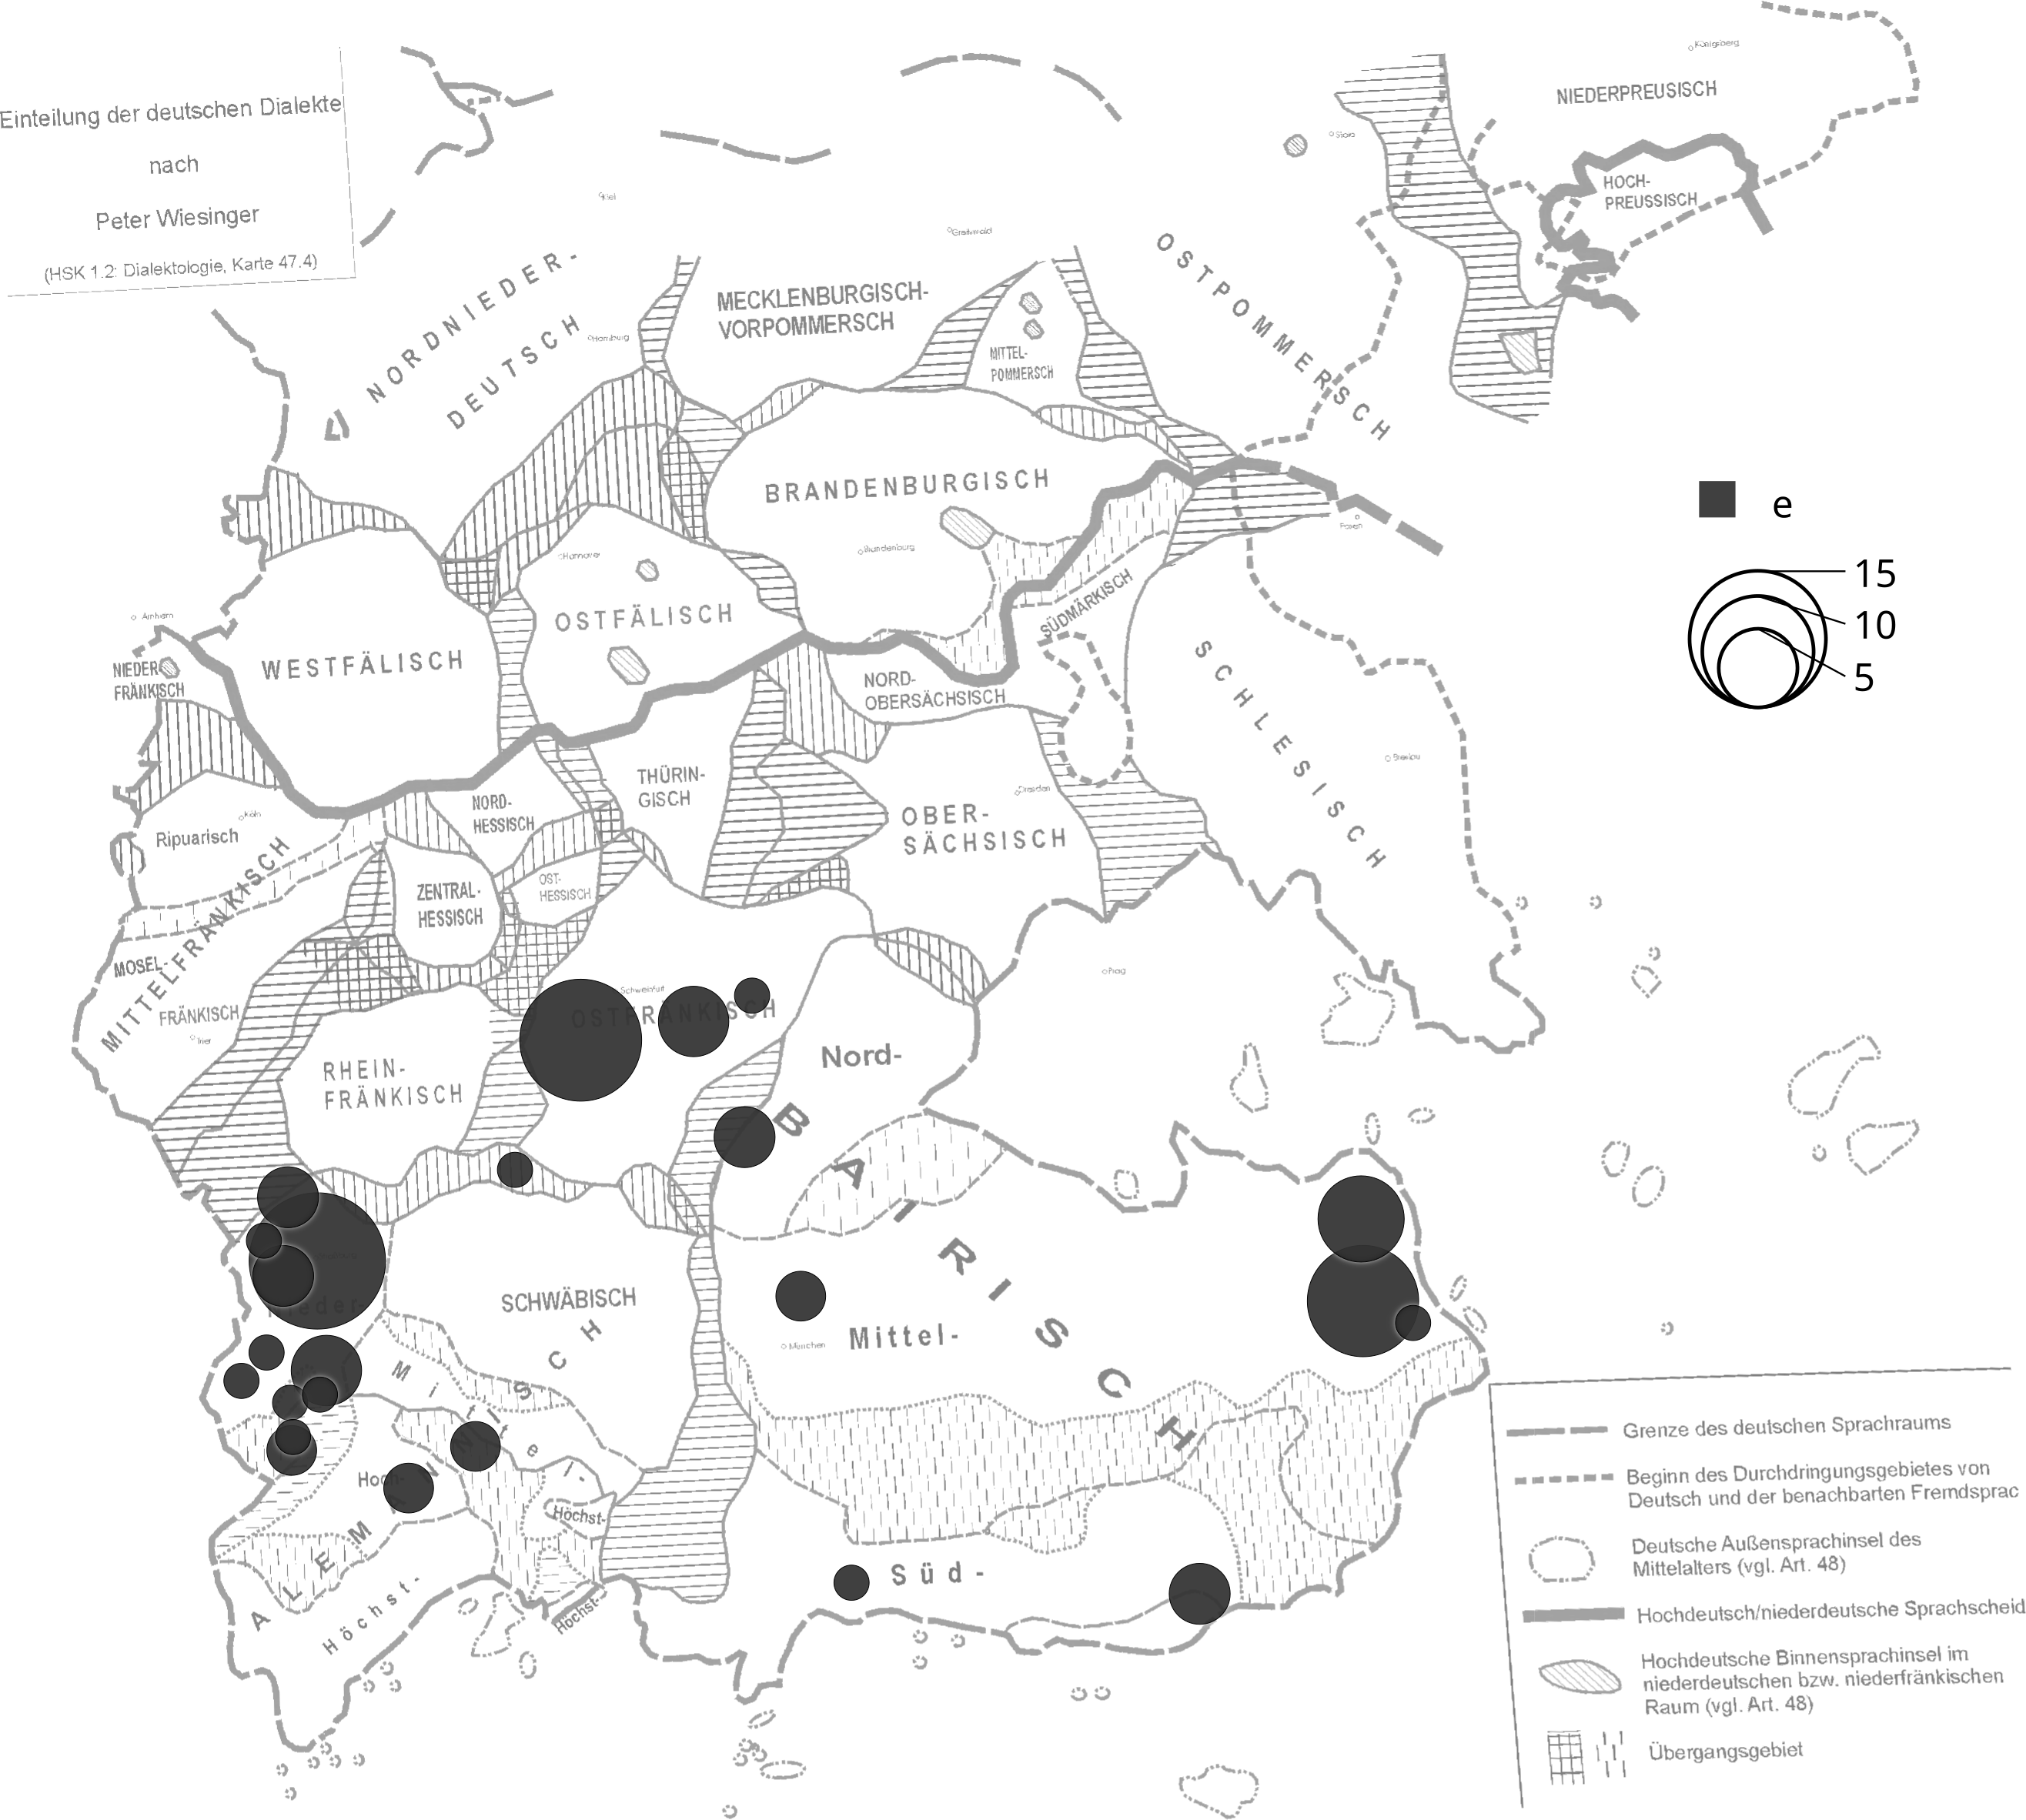
\includegraphics[
	width=\linewidth,
	keepaspectratio
]{./figures/2021-10-11_cao_beide-conj.png}
\caption{Geografische Distribution der Form \norm{bėide} in \norm{bėide \dots\ unde} `sowohl \dots\ als auch' (Hintergrundkarte: \cite{wiesinger1983:rede})}
\label{fig:cao_beideconj_geo_1}
\end{figure}

\begin{figure}
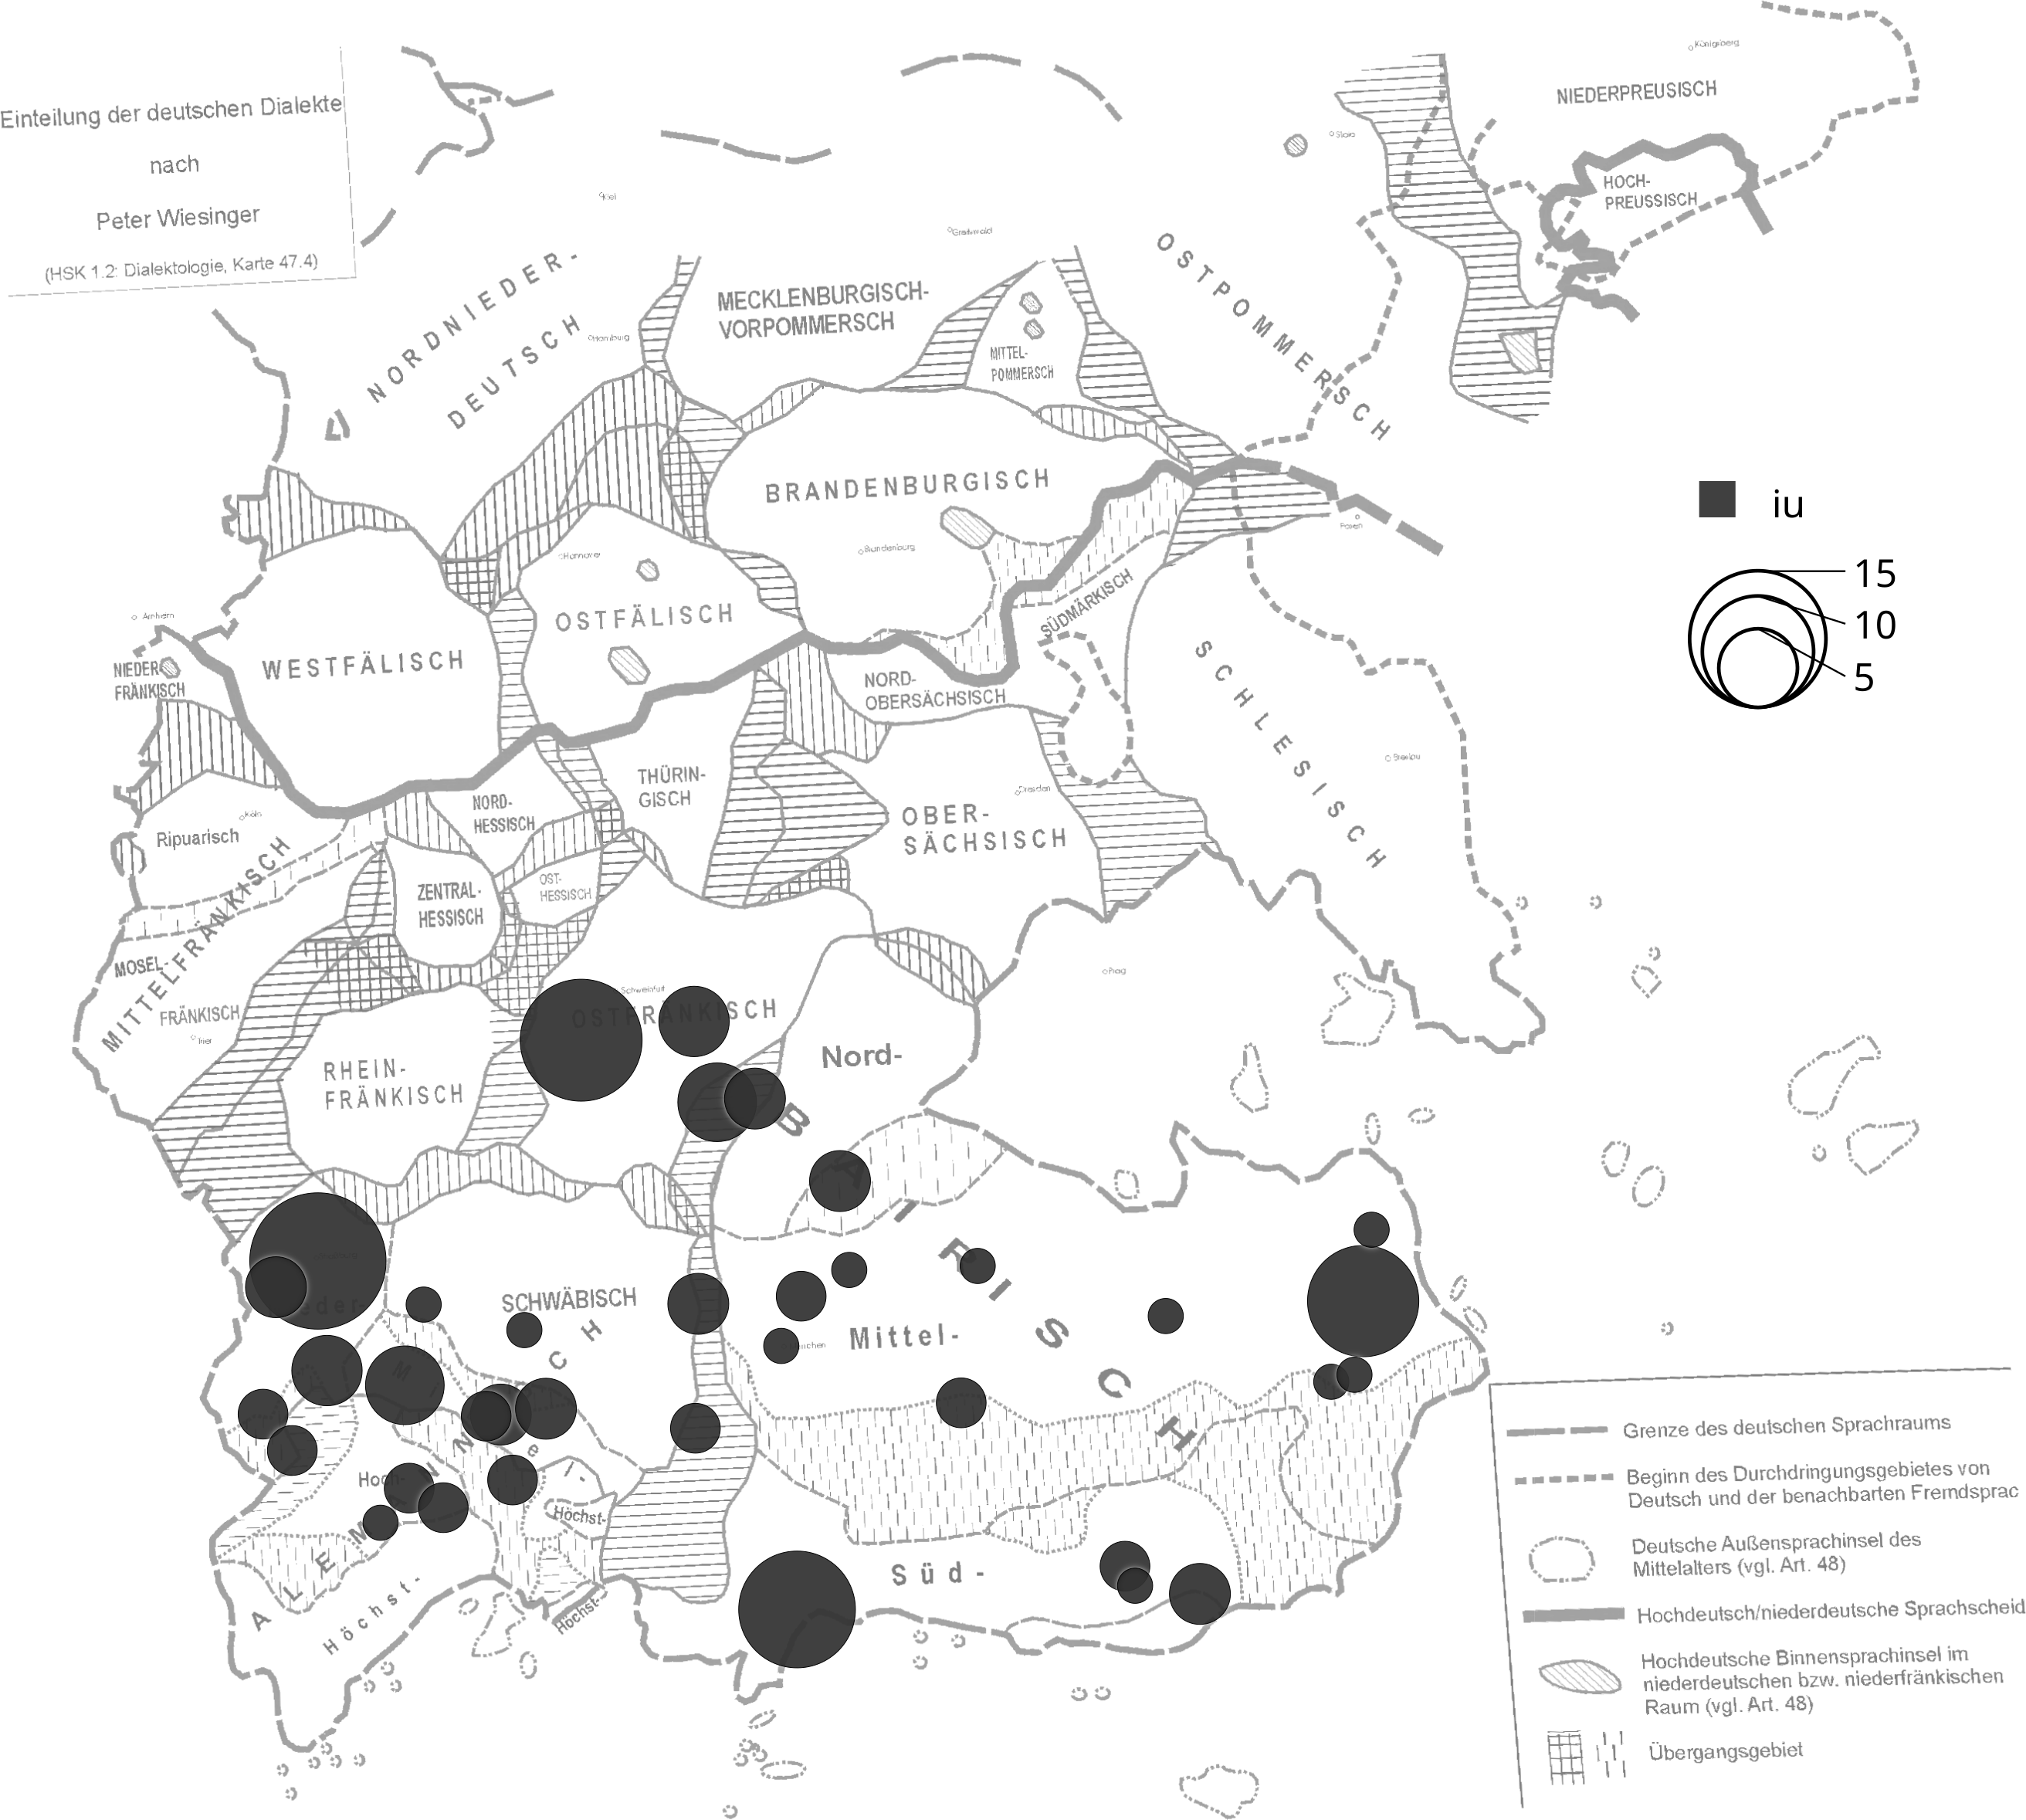
\includegraphics[
	width=\linewidth,
	keepaspectratio
]{./figures/2021-10-11_cao_beidiu-conj.png}
\caption{Geografische Distribution der Form \norm{bėidiu} in \norm{bėide \dots\ unde} `sowohl \dots\ als auch' (Hintergrundkarte: \cite{wiesinger1983:rede})}
\label{fig:cao_beideconj_geo_2}
\end{figure}

\citet{gjelsten1980} merkt an, dass es uneindeutige Fälle von \norm{bėide
\dots\ unde} gibt, die man \blockcquote[187]{gjelsten1980}{als appositive
Konstruktionen bewerten \textins{kann}, weil zwischen Pronomen und kopulativer
Fügung (Genus-)Kongruenz besteht, oder als konjunktionale Konstruktionen, weil
die Pronominalform als erstarrte konjunktionale Konstituente interpretierbar
ist}. Bei der Untersuchung haben sich im exzerpierten Material aber keine
Muster gezeigt, die eindeutig darauf hindeuten, dass bei der Annotation der
exzerpierten Belege regelmäßig Apposition und Konjunktion verwechselt worden
wären. Daneben liegen allerdings die zwei Belege in \REF{ex:kczbeidenundesynt1}
aus der \KC{}-Handschrift Z vor, in denen \norm{bėide} eindeutig als Dativ
flektiert erscheint.

\begin{exe}
\ex \label{ex:kczbeidenundesynt1}
\begin{xlist}
	\ex \label{ex:kczbeidenundesynt1_1}
		\gll Baiden man vnd wib \\
			beide-\textsc{dat.pl\subMF.st} Mann[\textsc{dat.sg.\MascM}] und
				Frau[\textsc{dat.sg.\NeutF}] \\
	\sn \gll Gebott er allen an den lyb \\
			gebot er all-\textsc{dat.pl\subMF.st} an den Leib \\
		\trans `Beiden, Mann und Frau, gebot er bei ihrem Leben'
			(%
				Z:~10va,9--10; vgl.~abweichend
				% C1:~3va,19--20; % beidev man vnd weip.
				% K:~3va,22--23; abweichend % [da]rzuͦ man vnd(e) wip
				% A1:~3va,1--2; % bediu wip unt man.
				% M:~5va,16--17; % Baidív wip vnd man.
				% H:~3vb,10--12; % Bede und(e) man.
				% B1:~3vc,51--53; % Baideu weip vnde man
				% VB:~3vb,5--7; % Beidiv wip vnd man
				% P:~6ra,8--10; % beide wip vnd(e) man.
				\KC:~V.~619--621;
				\cite[92]{schroeder1895}%
			)

\ex \label{ex:kczbeidenundesynt1_2}
	\gll Baiden man vnd wÿb \\
			beide-\textsc{dat.pl\subMF.st} Mann[\textsc{dat.sg.\MascM}] und
				Frau[\textsc{dat.sg.\NeutF}] \\
	\sn \gll Sol es gan an den lÿb \\
			soll es gehen an den Leib \\
		\trans `Beiden, Mann und Frau, soll es ans Leben gehen.'
			(%
				Z:~15ra,18--19; vgl.~abweichend
				% C1:~4vb,2; % baidev man vnd weip.
				% K:~4vb,33--34; zu % Baidu̍ man vnd(e) wip
				\KC:~V.~846--849;
				\cite[97]{schroeder1895}%
			)
\end{xlist}
\end{exe}

Da im Plural eine Form vom Typ \norm{wīben} zu erwarten wäre, wurden die
Substantive hier als generisch verwendete Singulare aufgefasst. Das
kataphorische \lit{Baiden} bezieht sich zusammenfassend auf die nachfolgenden
Konjunkte. Da \norm{bėide} die Zweizahl in seiner Bedeutung definiert, ist es
notwendig, dass die beiden singularischen Konjunkte \norm{man} `Mann' und
\norm{wīp} ihre \textsc{index}-Merkmale zu einem Plural vereinigen, damit ein
zusammenhängender und wohlgeformter Ausdruck entsteht. Im Dat.~Pl.\ der starken
Adjektivdeklination spielt Genus keine Rolle, insofern kann diese Kategorie
hier vernachlässigt werden. Ansonsten wäre jedoch mit Gender Resolution zu
rechnen. Da Apposition vorliegt, muss \norm{bėide} genauso wie die Konjunkte im
Dativ stehen. \lit{Baiden} verkörpert also zusammen mit dem konkretisierenden
\norm{man unde wīp} das indirekte Objekt von \lit{gebott} `gebot'
beziehungsweise \lit{sol} `soll'.

Im Rahmen der LFG deuten \citet{sadlernordlinger2006} appositive Strukturen als
Variante von Koordination ohne overte Konjunktion. Sie diskutieren dies anhand
von Beispielen aus verschiedenen australischen Sprachen, in denen Koordination
von NPs durch einfache Nebeneinanderstellung der Konjunkte erreicht wird.
Darüber hinaus werde Nebeneinanderstellung aber nicht nur für asyndetische
Koordination von NPs verwendet, sondern auch für eine Reihe anderer,
\q{Appositions-artiger} Konstruktionen
\autocite[440--441]{sadlernordlinger2006}. Für den vorliegenden Fall ist
lediglich wichtig, dass bei Koordination das \textsc{index}-Merkmal der
Konjunkte aufgelöst wird, bei Apposition hingegen nicht
\autocite[444]{sadlernordlinger2006}. Die Beispiele in
\REF{ex:kczbeidenundesynt1} lassen sich daher wie in
\figref{fig:kczbeidenundesynt2} dargestellt modellieren.

\begin{figure}
	\begin{forest} shorter edges, narrower nodes, italic leaves, align text
	[{\anno[\pass{\SObj{recip}}]{DP\mysn{beidenunde_DP}}}
		[{\anno[\updownelem]{QP}}
			[\anno{\xhead{Q}}
				[bėiden, name=beiden, minimum width=3em]
			]
		]
		[{\anno[\updownelem]{NP}}
			[{\anno[\updownelem]{\xhead{N}}}
				[man]
			]
			[Conj
				[unde]
			]
			[{\anno[\updownelem]{\xhead{N}}}
				[wīp]
			]
		]
	]
	%
	% Annotation des Knotens zu breit, als dass die AVM noch hinpasst
	\node at (beiden) [below=1ex] {
		\smaller[2]\upshape\tabcolsep=.5ex%
		\begin{tabular}[t]{@{} l l l @{}}
			\ups{gf~case} & \req & \textsc{dat} \\
			\ups{gf~num}  & \req & \textsc{pl} \\
		\end{tabular}%
	};
	%
	\node [avmcontainer=0ex, font=\footnotesize] {
		\avm{%
		\tikzmark{beidenunde_f}$f$: [
			conj	& \textit{appos} \\
			\mc{2}{l}{%
				\{
					$g_1$: [
						pred	& `beide'
					]~$i$, \smallskip \\
					%
					$g_2$: [
						conj	& \textit{g-und} \\
						\mc{2}{l}{%
							\{
								$h_1$: [
									pred	& `Mann' \\
									pers	& 3 \\
									num		& \textsc{sg} \\
									gend	& \textsc{m} \\
									sex		& \SM \\
									case	& \textsc{dat}
								],
								$h_2$: [
								 	pred	& `Frau' \\
								 	pers	& 3 \\
								 	num		& \textsc{sg} \\
								 	gend	& \textsc{n} \\
								 	sex		& \SF \\
								 	case	& \textsc{dat}
								]
							\}%
						} \smallskip \\
						%
						index	& [
							pers	& 3 \\
							gend	& \textsc{n} \\
							num		& \textsc{pl}
						]
					]~$i$
				\}%
		}\smallskip \\
		index	& [
				pers	& 3 \\
				gend	& \textsc{n} \\
				num		& \textsc{pl}
			] \\
		]}
	};
	\end{forest}
	
\begin{tikzpicture}[remember picture, overlay]
	\draw [myarrow]
		([yshift=.5ex]{pic cs:beidenunde_DP})
		to [out=east, in=north west]
		([yshift=.5ex]{pic cs:beidenunde_f});
	\end{tikzpicture}
	\caption{Analyse des Satzfragments \norm{bėiden, man unde wīp} `beiden,
		Mann und Frau'}
	\label{fig:kczbeidenundesynt2}
\end{figure}

In der F-Struktur auf der rechten Seite werden die Konjunkte \norm{man} `Mann'
und \norm{wīp} `Frau' in $g_2$ mit ihren grammatischen Eigenschaften einzeln
als $h_1$ und $h_2$ aufgelistet. Sie bilden zusammen einen neuen \textsc{index}
$i$, der die aufgelösten Personenmerkmale enthält. Sodann bildet $g_1$ mit
$g_2$ eine Apposition in $f$, wobei das Pronomen \norm{bėiden} in $g_2$ mit
$g_1$ koindiziert ist. Beide Teile zusammengenommen haben ihrerseits ein
\textsc{index}-Merkmal, das hier allerdings dem Index $i$ entspricht, da $g_1$
keine neuen Informationen hinzufügt. In der C-Struktur auf der linken Seite
bilden \norm{man unde wīp} zusammen eine NP, die wiederum zusammen mit der QP
\norm{bėiden} eine DP bilden, die als indirektes Objekt dient.

\chapter{Zusammenfassung und Ausblick}
\label{ch:zusammenfassung}

Die starke \isi{Adjektivdeklination} im oberdeutschen\il{Oberdeutsch}
Sprachraum\is{Dialektgeografie} der mittelhochdeutschen\il{Mittelhochdeutsch}
Periode macht im Nom.\ und Akk.\ Pl.\ noch einen Unterschied zwischen
Maskulinum und Femininum gegenüber dem Neutrum \autocite[182]{ksw2}. Die
Wortform des hier exemplarisch untersuchten determinierenden\is{Determinierer}
Quantors \norm{bėide} `beide' lautet daher je nach Kongruenzkontext
\norm{bėide} (Nom./Akk.\ Pl.\ M./F.\ stark) oder \norm{bėidiu} (Nom./Akk.\ Pl.\
N.\ stark).

Gerade beim kombinierten belebten\is{Animata} Bezug auf Referenten mit
unterschiedlichem \isi{Genus} beziehungsweise \isi{Sexus} -- männlich und
weiblich als grammatikalisierte semantische Geschlechterkategorien der
Animata~-- ist aber in der Regel die formal neutrale Form zu finden. Diese Art
von \q{Auflösungsphänomen}\is{Gender Resolution}, das bei konfligierenden
Genus-\is{Genusmerkmal} oder Sexusmerkmalen\is{Sexusmerkmal} von kombinierten
Personenmerkmalen\is{Personenmerkmal} auftritt, wird als
\fw{\isi{Gender Resolution}} bezeichnet
\autocites{corbett1983}[264--306]{corbett1991}. Da jedoch auch Fälle zu
beobachten sind, in denen in diesem Kontext die formal maskulin-feminine Form
auftritt, wurde in dieser Arbeit der Frage nachgegangen, wie häufig die
jeweiligen Formen in verschiedenen syntaktischen Kontexten auftreten und welche
Parameter einen Einfluss auf das Erscheinen der einen oder anderen Form haben.
Darüber hinaus bestand die Frage, wie sich \norm{bėide} in der koordinierenden
Konstruktion \norm{bėide \dots\ unde} `sowohl \dots\ als auch' im Vergleich zu
quantifizierendem \norm{bėide} verhält.

Die älteren Grammatikwerke zum Mittelhochdeutschen\il{Mittelhochdeutsch}
\autocites[384]{paul2007}[187--189, 222]{dal2014}[258]{michels1979}%
[221]{mettke2000} machen zu beiden Aspekten nur sehr pauschale Aussagen.
\citet[621--628]{ksw2} gehen zwar auf die möglichen syntaktischen Kontexte des
Quantors \norm{bėide} und deren Häufigkeit\is{Frequenz} in ihrem \isi{Korpus}
sowie auf die geografische\is{Dialektgeografie}
Distribution\is{Distribution!geografische} der Formen der \isi{Konjunktion}
\norm{bėide} ein. Sie machen aber keine Angaben zur Variationsbreite zwischen
den Formen in den verschiedenen Kontexten sowie deren steuernde Faktoren;
letzterer Aspekt wäre für den derzeit ausstehenden Band zur Syntax zu erwarten.

Darüber hinaus stehen zwar zwei Studien zum hier untersuchten Themenkomplex von
\citet{askedal1973,askedal1974} zur Verfügung, doch dienen ihm für die
mittelhochdeutsche\il{Mittelhochdeutsch} Periode (ca.~1050--1350) textkritische
Editionen\is{Editionsphilologie} lediglich zweier prominenter Verstexte der
Artusepik als Quelle. Seine Schlussfolgerungen zum
konjunktionalen\is{Konjunktion} Gebrauch von
\norm{bėide} \autocite{askedal1974} sind zudem fragwürdig und beschränken sich
auf nominale Konjunkte \autocite{gjelsten1980}.

Die Idee dieser Arbeit war daher, sowohl den Quantor als auch die
\isi{Konjunktion} \norm{bėide} auf einer handschriftennahen und zumindest
synchron breiteren Basis als die Arbeiten von \citet{askedal1973,askedal1974}
zu untersuchen. Als Textgrundlage dienten zum einen das
\citefield{cao1}[citetitle]{maintitle} (\CAO{};
\nosh\cites{cao1,cao2,cao3,cao4,caor,cao5}) als Sammlung von alltagsnahen
Gebrauchstexten\is{Gebrauchssprache} in Prosa\is{Prosa} vor allem des späten
13.~Jahrhunderts und zum anderen die Haupthandschriften der \citetitle{kc}
(\KC{}; vgl.~\cites{schroeder1895,nellmann1983}) als erzählerisch
ausgestalteter Sachtext in Versform, der hauptsächlich im 13.\ und 14.\
Jahrhundert breit über\-liefert ist. Diese Texte haben den Vorteil, dass sie
digital in diplomatischer \isi{Transkription} vorliegen. Dies vereinfacht die
Belegsammlung enorm, gerade auch, weil das hauptsächlich untersuchte Phänomen,
mittelhochdeutsch \norm{bėide} `beide' in Bezug auf zwei Referenten, nicht
ausgesprochen häufig auftritt.

Für das \CAO{} beträgt die Frequenz\is{Frequenz} von \norm{bėide} und
\norm{bėidiu} zusammen ca.~282 Vorkommen pro 1~Mio. Wortformen, für die \KC{}
ca.~510 Vorkommen pro 1~Mio. Die Texte des \CAO{} und der \KC{} wurden mit
Hilfe von regulären Ausdrücken\is{regulärer Ausdruck} durchsucht und
anschließend manuell annotiert \autocites[vgl.\
z.\,B.][33--37]{perkuhnetal2012}[zur Methode
vgl.][207--209]{beckerschallert2021}[155--158]{beckerschallert2022b}. Der
Umstand, dass die Urkunden\is{Urkunde} häufig dem engeren Umkreis eines
bestimmten Ausstellungs\-orts zugeordnet werden können, erlaubt einen
zusätzlichen Blick auf die geografische\is{Dialektgeografie} Dimension der
beobachteten Variation.
% Dies ermöglicht prinzipiell einen schreibdialektalen Vergleich mit
% literarischen Handschriften, deren regionale Herkunft in der Regel nur
% indirekt erschlossen werden kann.

%%%%%%%%%%%%%%%%%%%%%%%%%%%%%%%%%%%%%%%%%%%%%%%%%%%%%%%%%%%%%%%%%%%%%%%%%%%%%%%

\section{Ergebnisse}

In einer vorbereitenden Untersuchung der zahlenmäßig größten Ausstellungs\-orte
und ihrer näheren Umgebung sowie zu den auszuwertenden Handschriften der
\KC{} anhand einiger im Material häufig belegter Adjektive wurde
sichergestellt, dass am jeweiligen Ort oder in der jeweiligen Handschrift
grundsätzlich ein Unterschied in der Flexion zwischen \norm{\mbox{-e}} und
\norm{-iu} vorhanden ist. Dies steht vor dem Hintergrund des Abbaus der
Genusdistinktion\is{Genusdistintion, Abbau der} im Plural der
\isi{Adjektivdeklination} zum Frühneuhochdeutschen\il{Frühneuhochdeutsch} hin
\autocite[191--192]{reichmannwegera1993}, deren Wirken sich jedoch weder im
\CAO{} noch in den meisten \KC-Handschriften stark bemerkbar gemacht hat.
Ausnahmen bilden Straßburger Urkunden und die \KC{}-Handschrift Z.%
%
	\footnote{Die Siglen der \KC-Handschriften richten sich nach
		\citetitle{kcdigital}, siehe \citeurl{kcdigital}.}

Die \KC{}-Handschriften wurden jeweils nach Eindeutigkeit und Vorkommen der
Opposition im jeweiligen syntaktischen Kontext in verschiedene Gruppen
eingeteilt, um sie in ihrer Relevanz für die Untersuchung zu priorisieren. Zur
Auswertung des Quantors \norm{bėide} dienten hauptsächlich die Handschriften
B1, C1, K und VB; bei der \isi{Konjunktion} \norm{bėide} kamen vor allem A1, B1
und VB zum Zug. Gerade die Vorauer Handschrift (A1) als bedeutendste
\KC{}-Handschrift fand bei der Auswertung zum Quantor \norm{bėide} also keine
Verwendung, da dort für diesen Kontext nahezu ausschließlich maskuline
\isi{Controller} belegt sind. Dies stellte generell bei der Auswertung der
\KC{} eine Herausforderung dar, die sich auf die Thematik des Texts
zurückführen lässt.

Die beiden Auswertungsserien sind prinzipiell miteinander vergleichbar. Die aus
der \KC{} exzerpierten Belege, wenn auch geringer in der Anzahl, verhalten sich
nicht grundlegend anders als die aus dem \CAO{} gewonnenen. Allerdings wurden
für die \KC{} aufgrund der von \citet[89--90]{askedal1973} und
\citet[191]{gjelsten1980} geäußerten Vorbehalte\is{Vorbehalt} solche Kontexte
nicht gewertet, in denen \norm{bėide} am \isi{Versende} oder vor einem Wort
steht, das mit einem Vokal beginnt. Sie sprechen diesbezüglich von
Neutralisierungs\-positionen. Für das \CAO{} wurden Belege im letzteren Kontext
ebenfalls zunächst unter Vorbehalt betrachtet für den Fall, dass dieser auch
auf Prosatexte\is{Prosa} zutrifft, wie \citet[92]{askedal1973} zu bedenken
gibt. Jedoch ließ sich für die Prosatexte kein Unterschied zu
Nicht-\allowbreak{}\isi{Hiatus}-\allowbreak{}Belegen feststellen.
\citeauthor{askedal1973}s Einwand ist also zumindest für das \CAO{}
zurückzuweisen.

\subsection{\norm{Bėide} als Quantor: Animata}
\is{Animata|(}

Die Funktion von \norm{bėide} als Quantor betreffend stimmt die Mehrzahl der
gesammelten Belege zu belebten Referenten mit der bereits von
\citet[312]{grimm1890} und \citet[39--41]{behaghel1928} formulierten
Beobachtung überein, dass beim Bezug auf zwei Referenten mit gleichem
\isi{Genus} die maskulin-feminine Form steht, während in Bezug auf Referenten
mit unterschiedlichem \isi{Genus} das Neutrum auftritt. Dies gilt allerdings
auch zum Beispiel für den Bezug auf Pronomen der ersten und zweiten Person, die
formal keine overte Genuskategorie\is{Genusmarkierung} besitzen, diese
Informationen aber in ihrer referentiellen Semantik beinhalten. Generell gilt,
dass beim kombinierten Bezug auf belebte Referenten deren semantisches
Geschlecht (\isi{Sexus}) beziehungsweise die damit assoziierten
Resolutionsregeln im Großteil der Fälle die Kongruenzform bestimmen.

Betreffend der \isi{Distribution!syntaktische} der syntaktischen Kontexte ist
mit \citet[624, Abbildung P~179]{ksw2} übereinstimmend
anzumerken\is{Validierung}, dass der unmittelbare Bezug von \norm{bėide} auf
zwei \isi{Controller} in beiden Auswertungsserien sehr selten auftritt. In
nahezu allen der wenigen belegten Fälle liegt in diesen Kontexten
\isi{Distanzstellung} vor (\norm{\emph{N\tsub{i}} unde \emph{N\tsub{j}} \dots\
bėide}), was die Wortabfolge\is{Abfolge} betrifft. Der mittelbare Bezug auf
zwei \isi{Controller} über mindestens ein Pronomen macht den Großteil der
Belege aus (\isi{Kontaktstellung}: \norm{\emph{PRO\tsub{i+j}} bėide};
\isi{Distanzstellung}: \norm{\emph{PRO\tsub{i+j}} \dots\ bėide}).
Genus\-indifferentes\is{Genusindifferenz} \norm{si} `sie' stellt gefolgt von
\norm{wir} `wir' den häufigsten unmittelbaren \isi{Controller} von \norm{bėide}
dar.

Historisch\is{Diachronie} ist zwar im Nom./Akk.\ bei den
Personalpronomina\is{Personalpronomen} der 3.~Pers.\ Pl.\ mit der
Genus\-opposition \norm{sie} `sie (\textsc{m+f})' gegenüber \norm{siu} `sie
(\textsc{n})' zu rechnen. Eine stichprobenhafte\is{Stichprobe} Teilauswertung
hat ergeben, dass in den hier untersuchten Materialien dieser Unterschied in
aller Regel aber schon nicht mehr nachvollziehbar ist, also generell \norm{si}
steht, landschaftlich auch eine Form vom Typ
\norm{sei},
\norm{seu},
\norm{sie} oder
\norm{siu}
\autocites[vgl.][213--214]{paul2007}[369, 390--397]{ksw2}[482--483]{wmu1}.
\posscite[99]{askedal1973} Behauptung, dass \norm{si bėide} eine
Konstruktion bildet, bei der das Neutrum immer nur an einem der beiden Glieder
markiert wird (\q{Monoflexion}), kann für das ausgewertete Material daher
nicht nachvollzogen werden.

Gerade in \isi{Kontaktstellung} zu Personalpronomina\is{Personalpronomen} wurde
bei belebtem Bezug die höchste Variation zwischen \norm{bėide} und
\norm{bėidiu} beobachtet. Die Begründung dafür wurde in der Annahme gesucht,
dass für die Auflösung\is{Gender Resolution} des Bezugs auf \isi{Controller}
mit gemischtem Geschlecht entweder formale\is{Kongruenz!formale}
(\textsc{m}~∨~\textsc{f} $\Rightarrow$~\norm{-e}) oder semantische
Kongruenz\is{Kongruenz!semantische} (\SM{}~∩~\SF{} $\Rightarrow$~\norm{-iu}) in
Frage kommt, falls \norm{si} und \norm{bėide} eine syntaktische Phrase bilden.
Das Pronomen gibt nämlich in diesen Fällen selbst keine formalen
Genus\-merk\-male (mehr) vor, die per \isi{Concord} verfügbar wären. Etwa drei
Viertel der Targets\is{Target} mit gemischtgeschlechtlichem Bezug
(belebt\is{Animata} und unbelebt\is{Inanimata}) im \CAO{} weisen in diesem
Kontext \isi{Gender Resolution} auf. Die insgesamt bedeutend geringere
Belegzahl in der \KC{} ist für sich genommen nicht aussagekräftig, verhält sich
aber konform zu den \CAO-Belegstellen.

Bei eindeutiger \isi{Distanzstellung} des Targets\is{Target} wurde für das
\CAO{} beobachtet, dass regel\-mäßig Gender Re\-solu\-tion vorliegt, wenn sich
\norm{bėide} auf kombinierte Controller bezieht, also nicht auf einen
einzelnen, eindeutigen lexikalischen Phrasenkopf\is{Kopf} beziehungsweise das
modifizierte Pronomen kein explizites Genusmerkmal bereitstellt, mit dem
formale Kongruenz\is{Kongruenz!formale} möglich ist. Unter der Hypothese, dass
das Neutrum generell mit \isi{Inanimata} und, im Umkehrschluss, die
maskulin-feminine Form mit Animata assoziiert wird
\autocite[243--245]{askedal1973}, ist eine auffällige Zunahme von \norm{bėide}
mit belebter kombinierter Referenz bei steigendem
Wortformenabstand\is{Distanz!lineare} nicht zu beobachten. Ohnehin stellte sich
lineare Distanz\is{Distanz!lineare} nicht als ausschlaggebender Faktor für die
beob\-ach\-tete Variation heraus.

In wenigen Fällen tritt in beiden Auswertungs\-serien beim belebten, männlichen
Bezug die neutrale Form auf, ohne dass dafür eine systematische Motivation
gefunden werden konnte. \citet{wechslerzlatic2003} und \citet{wechsler2009}
modellieren \isi{Gender Resolution} bei Animata mit einer
Schnittmengenoperation zwischen den Sexusmerkmalen\is{Sexusmerkmal} der
involvierten Referenten. Zwei männliche Referenten bilden eine Schnittmenge,
die regelmäßig auf formaler Ebene das Maskulinum auslöst -- bis auf die
genannten Ausnahmefälle.

\is{Animata|)}

\subsection{\norm{Bėide} als Quantor: Inanimata}
\is{Inanimata|(}

Bei unbelebtem gemischten Bezug erfolgt noch regelmäßiger als bei den
Animata\is{Animata} die Auflösung\is{Gender Resolution} zum Neutrum. Allerdings
tritt auch hier die Form \norm{bėidiu} im \CAO{} mehrfach mit Bezug auf
kombinierte maskuline \isi{Controller} auf, und zwar etwas häufiger als die
erwartete Form \norm{bėide}. Für diese Kombination liegen aber insgesamt nur
sechs Belege vor; kombinierte feminine \isi{Controller} sind im Belegmaterial
keine vorhanden.

In allen anderen Fällen verhalten sich die
mittelhochdeutschen\il{Mittelhochdeutsch} Belege wie von
\citet{wechslerzlatic2003} und \citet{wechsler2009} für das
Isländische\il{Isländisch} beschrieben. Das Neutrum stellt in den untersuchten
mittelhochdeutschen\il{Mittelhochdeutsch} Texten das \isi{Default} dar. Es
tritt immer dann ein, wenn keine Schnittmenge zwischen den jeweiligen
Genusmerkmalen\is{Genusmerkmal} der zu kombinierenden \isi{Controller} und der
Menge der grammatikalisierten semantischen Genera\is{Genus} (G\tsub{s})
gebildet werden kann.

Der Ausnahmefall\is{Ausnahme} mit dem Neutrum als Kongruenzform bei
kombinierten Maskulina (sowohl belebten\is{Animata} als auch
unbelebten\is{Inanimata}) kann mit diesem Ansatz nicht erklärt werden.
Anzunehmen ist, dass die Defaultform\is{Default} als solche
übergeneralisiert\is{Generalisierung} auch auf ansonsten unproblematische
Kontexte mit kombinierter Referenz angewendet wird. Diese Möglichkeit wird von
\citet[302]{corbett1991} angeführt, allerdings im Rahmen seiner Untersuchungen
zum
Bosnisch-\allowbreak{}Kroatisch-\allowbreak{}Mazedonisch-\allowbreak{}Serbischen
(\ili{BKMS}) nur auf Inanimata bezogen
\autocites[vgl.~auch][190]{wechslerzlatic2003}[581]{wechsler2009}.

\is{Inanimata|)}

\subsection{\norm{Bėide} als Konjunktion}
\is{Konjunktion|(}
\is{Koordination|(}

Neben seiner Funktion als Quantor tritt `beide' im
Mittelhochdeutschen\il{Mittelhochdeutsch} auch als Teil der korrelativen
Konjunktion \norm{bėide \dots\ unde} `sowohl \dots\ als auch' auf. In beiden
Auswertungs\-serien, \CAO{} und \KC{}, treten als Konjunkte in dieser
Konstruktion verschiedene Phrasen\-typen und Wort\-arten auf: solche, die
selbst \isi{Controller} sind; solche, die Kongruenztargets\is{Target}
darstellen; und schließlich solche, die Personenmerkmale\is{Personenmerkmal}
weder definieren noch widerspiegeln.

Die Tatsache, dass \norm{bėide} in den
mittelhochdeutschen\il{Mittelhochdeutsch} Belegen auch mit letzteren vorkommt,
wurde als Evidenz für die weit fortgeschrittene \isi{Grammatikalisierung} der
Konstruktion angesehen. Der Verwendungskontext\is{Pragmatik} von \norm{bėide}
`beide' ist in diesem Zusammenhang nicht auf seine Bedeutung als Quantor von
Nominalen beschränkt, sondern wurde auf andere syntaktische Zusammenhänge
ausgeweitet. \norm{Bėide} dient hier als \isi{Fokuspartikel}, die die parallele
Gültigkeit der zwei genannten Optionen betont, nicht mehr als pronominal
verwendeter Quantor, der sich kataphorisch\is{Katapher} auf seine Referenten
bezieht und deren Zweizahl betont.

Bereits für das Spätalthochdeutsche\il{Althochdeutsch} lassen sich Belege
finden, die einen Übergang\is{Ambiguität} zwischen beiden Verwendungsarten
andeuten \autocite[vgl.\ die Beispiele in][627]{ksw2}. Entsprechend der
Grammatikalisierungstheorie\is{Grammatikalisierung} nach
\citet[146--150]{lehmann2015} geht der Wandel von einem freien Morphem zu einem
funktionalen typischerweise mit dem Verlust von paradigmatischer
Variabilität\is{Paradigma} einher. Es überrascht daher nicht, dass \norm{bėide}
in diesem Kontext erstarrt erscheint, also keine klare Abhängigkeit von den
Personenmerkmalen\is{Personenmerkmal} der Konjunkte ausgemacht werden konnte,
falls solche vorhanden sind. Stattdessen deutete sich an, dass die
geografische\is{Dialektgeografie} Verteilung\is{Distribution!geografische}
einen wichtigeren Faktor darstellt. Während \norm{bėidiu} im ganzen
oberdeutschen\il{Oberdeutsch} Sprachgebiet auftritt, liegen Belege für
\norm{bėide} hauptsächlich an dessen Rändern vor. Die Ergebnisse stimmen mit
den Angaben von \citet[627--628]{ksw2} überein.\is{Validierung}

\is{Konjunktion|)}
\is{Koordination|)}

%%%%%%%%%%%%%%%%%%%%%%%%%%%%%%%%%%%%%%%%%%%%%%%%%%%%%%%%%%%%%%%%%%%%%%%%%%%%%%%

\section{Ausblick}
\is{Desiderat|(}

Generell wäre in dieser Arbeit wünschenswert gewesen, für alle möglichen
Kombinationen von Genera\is{Genus} in allen syntaktischen Kontexten mehrere
Belege zur Verfügung zu haben. Dass sich dieser Wunsch nicht erfüllt hat, ist
eine Konsequenz der grundlegenden Herausforderung im Umgang mit historischen
Texten entsprechend dem \citeauthor{labov1994}'schen Diktum, dass die
historische Sprachwissenschaft die Kunst sei, den besten Nutzen aus schlechten
Daten zu ziehen.%
%
	\footnote{\foreignblockcquote{english}[11]{labov1994}{Historical
		linguistics can \textelp{} be thought of as the art of making the best
		use of bad data}.%
	}
%
Die \isi{Überlieferung} ist letztlich dem Zufall unterworfen und
fehlerbehaftet. Evidenz kann nur indirekt erhoben werden, da es keine
Muttersprachlerinnen und Muttersprachler gibt, die gezielt befragt werden
können \autocite[11]{labov1994}. Gerade digitale
Transkriptionen\is{Transkription} erleichtern es aber enorm, an Belege und
Beispiele zu kommen, selbst wenn keine morphologische oder sogar syntaktische
Annotation\is{Annotation} vorliegt.
% %
% 	\footnote{Darüber hinaus zeigt zum Beispiel die Arbeit von
% 		\citet{farrisarora2021}, dass schon einfache dependenzgrammatische
% 		Annotationen hilfreich sein können, um gezielt Belege für bestimmte
% 		syntaktische Kontexte zu finden, besonders auch für anscheinend
% 		seltenere syntaktische Kontexte wie \norm{bėide} in Bezug auf zwei
% 		Feminina.%
% 	}
% %
Für sprachgeschichtliche\is{Sprachgeschichte} Untersuchungen ist daher
wünschenswert, Transkriptionen\is{Transkription} digital verfügbar zu machen,
wenn sie im Rahmen von Editionsvorhaben\is{Editionsphilologie} ohnehin
anfallen.

Bei der Arbeit an dieser Untersuchung wurde deutlich, wie wichtig eine
sorgfältige Material\-auswahl ist. Es gilt zu bedenken, welche möglichen
morphologischen Kontexte von dem (oder den) untersuchten Text(en) ihrem Inhalt
gemäß abgedeckt werden können. Die Urkunden\is{Urkunde} des \CAO{} haben sich
an dieser Stelle als sehr geeignet erwiesen, da der Genusunterschied in der
Pluralflexion auf das Oberdeutsche\il{Oberdeutsch} begrenzt ist und das
Urkundenkorpus gerade diesen Raum\is{Dialektgeografie} dicht abdeckt. Darüber
hinaus fungieren nicht selten Paare aus Mann und Frau als Aussteller. Die
Wortformen \norm{bėide} und \norm{bėidiu} kommen häufig genug vor, dass eine
größere Belegmenge mit Hilfe von regulären Ausdrücken\is{regulärer Ausdruck}
manuell durchsucht und annotiert werden konnte, andererseits aber selten genug,
dass eine möglichst exhaustive Auswertung in dieser Form möglich war.

Die \KC{} stellte dagegen für die Belegsammlung eine Herausforderung dar, weil
aufgrund ihres Inhalts kaum Paare aus Mann und Frau gemeinsam auftreten, obwohl
einzelne Episoden explizit eine Protagonistin besitzen. Möglicherweise wäre es
aufschlussreicher gewesen, die verschiedenen Textzeugen eines ähnlich breit
überlieferten, erzählenden Texts zu untersuchen -- insofern sie als digitale
Transkriptionen\is{Transkription} verfügbar sind. Zum Beispiel bietet sich
neben einer Erweiterung von \posscite{askedal1973,askedal1974} Auswertung des
\tit{Tristan} und des \tit{Parzival} auf ihre einzelnen Textzeugen prinzipiell
auch der \tit{Iwein} Hartmanns von Aue an, dessen \isi{Überlieferung} 33
derzeit bekannte Textzeugen umfasst \autocites[vgl.][s.\,v.~\textit{Hartmann
von Aue: \tit{Iwein}}]{hsc}.%
%
	\footnote{Transkriptionen\is{Transkription} der einzelnen Textzeugen des
		\tit{Iwein} werden im Rahmen von \citetitle{iwdigital} verfügbar
		gemacht, siehe unter \citeurl{iwdigital}. Zum \tit{Parzival} siehe das
		Berner \tit{Parzival}-Projekt unter \citeurl{parzivalprojekt}.%
	}

Phänomene im Rahmen von Spaltungskonstruktionen wie zum Beispiel der
Bedeutungs\-unterschied zwischen der \isi{Kontaktstellung} und der
\isi{Distanzstellung} von Quantoren sind eine interessante Fragestellung in
Hinsicht auf ihre formal\-syntaktische Modellierung \autocite[siehe
z.\,B.][]{pittner1995,merchant1996,fanselowcavar2002,nolda2007,shen2019}. In
der vorliegenden Auswertung deutete sich an, dass im auch
Mittelhochdeutschen\il{Mittelhochdeutsch} ein grammatischer Unterschied
vorliegt, der sich in der anscheinend höheren Affinität zu semantischer
Kongruenz beim distanten Quantor äußert. Denkbar wäre eine Folgestudie, die
explizit \q{problematische} \isi{Controller}\is{Ausnahme} in diesem Kontext
betrachtet, zum Beispiel Lexical Hybrids\is{Lexical Hybrid} wie \norm{wīp}
`Frau (\NeutF)', und sie mit \q{unproblematischen} Substantiven\is{Substantiv}
vergleicht. Bezüglich des Bindungsverhaltens\is{Bindung} von Floating
Quantifiers\is{Floating Quantifier} wäre genereller auch der Vergleich mit
Reflexivpronomina\is{Reflexivpronomen} und prädikativen
Adjektiven\is{Adjektiv!prädikativ} interessant, da auch sie sich im
\isi{Mittelfeld} befinden und mit Subjekten koindiziert\is{Koindizierung} sind.
Weiterhin könnte es lohnend sein, die Überlegungen von \citet{spector2009} zur
Spaltung von Topik-\is{Topik} und Subjektfunktion in Konstruktionen mit
\isi{Floating Quantifier} näher zu untersuchen, auch was die Modellierung des
Objektbezugs durch den Quantor betrifft.

Darüber hinaus kam zur Sprache, dass sich im Plural der starken
\isi{Adjektivdeklination} zum Neuhochdeutschen\il{Neuhochdeutsch} hin das
Flexiv \norm{-e} auf alle Genera\is{Genus} ausbreitet
\autocite[vgl.][191--192]{reichmannwegera1993}. Bereits \citet{askedal1973}
stellt dies in den Kontext der Numerusprofilierung\is{Genusdistinktion, Abbau
der}. \citet{dammelgillmann2014} behandeln diesbezüglich die \isi{Diachronie}
des morphologischen Systems der Substantive\is{Substantiv}, allerdings sind
auch Adjektive\is{Adjektiv!attributiv} als Modifikatoren\is{Modifikator} von
Substantiven Teil des Nominalkomplexes. Zu untersuchen wäre also, wie sich in
ihrem Ansatz die Ausbreitung der maskulin-femininen Flexionsendung in den
größeren Kontext des Umbaus der Nominal\-flexion einfügt.

\is{Desiderat|)}

Vieles könnte im Rahmen dieser Untersuchung noch gesagt und präzisiert werden,
doch möchte ich an dieser Stelle einen vorläufigen Punkt setzen und mit Ishmael
schließen: \foreignblockquote{english}[{Herman Melville: Moby-Dick;
\cite[159]{melville:mobydick}}]{It was stated at the outset, that this system
would not be here, and at once, perfected. You cannot but plainly see that I
have kept my word.
% But I now leave my cetological System standing thus unfinished, even as the
% great Cathedral of Cologne was left, with the crane still standing upon the
% top of the uncompleted tower. For small erections may be finished by their
% first architects; grand ones, true ones, ever leave the copestone to
% posterity.
\textelp{}
God keep me from ever completing anything. This whole book is but a
draught---nay, but the draught of a draught}. % (Schluss von Kapitel 32)


\appendix
\part*{Anhang}
\addcontentsline{toc}{part}{Anhang}
\chapter{Liste der gesichteten Urkunden}
\label{sec:urkliste}
\is{Stichprobe|(}

Die folgenden zwei Listen enthalten die Urkundennummern im \tit{Corpus der
altdeutschen Originalurkunden} (\CAO), die für die Auswertung gesichtet wurden.
Dabei sind nicht sämtliche Urkunden in die Auswertung eingeflossen, da nicht
alle Belege für das untersuchte Phänomen enthalten. Überschneidungen mit dem
\tit{Referenzkorpus Mittelhochdeutsch} (\REM; \nosh\cite{rem}) und der
\tit{Mittelhochdeutschen Grammatik} von \citet{ksw3,ksw2} sind durch
Kursivierung gekennzeichnet.

\section{Ausgewertete Urkunden}
\label{subsec:ausgewurk}

Die hier aufgelisteten Urkundennummern sind in die Stichprobe zur Auswertung von
\norm{bėide} \wdef{beide} eingeflossen, da sie relevante Belegstellen
enthielten.

{%
\setlength{\columnsep}{35pt} % Aus langscibook.cls geschlossen (\p@ = 1.0 pt)
\raggedright
\begin{multicols}{2}
\begin{description}[
	font=\normalfont,
	labelsep=\fontdimen2\font,
	leftmargin=1.4cm, % Ebenfalls aus langscibook.cls übernommen
]
\item[\cite{cao1},] 31, \emph{75}, \emph{76}, 81, \emph{85}, 86, 131, 165, 171,
179, 190, 199, 201, 214, 260, 326, 371, 389, 415, \emph{429}, 491, \emph{508},
519, 524, 559, \emph{560}

\item[\cite{cao2},] 583, 604, 610, 619, 627, 629, 632, 636, 656, 682, 701, 777,
885, 923, 925, 937, 971~A, 971~B, 1001, 1055, 1073, 1121, 1126~A, 1126~B, 1137,
1153, 1154, 1201~A, 1201~B, 1217, 1218, 1221, 1229, 1234, 1259, 1270, 1282,
1304, 1352, 1359, 1382, 1414, 1416, 1429, 1436, 1503, 1504, 1514, 1545, 1566,
1568, 1578, 1584, 1620, 1657

\item[\cite{cao3},] 1661, 1747, 1764, 1802, 1831, 1843, 1898, 1950, 1956, 1971,
1972~A, 1972~B, \emph{2001}, 2005, 2011, 2055, 2092, 2110, 2174, 2183, 2214,
2240, 2253, 2293, 2307, 2309, 2310, 2338~A, 2338~B, 2350, 2353, 2359, 2367,
2375, 2396, 2401, 2406, 2412, 2445, 2468, 2497, 2532, 2535

\item[\cite{cao4},] 2563, 2568, 2583, 2625~A, 2625~B, 2651~A, 2651~B, 2694,
2713, 2719, \emph{2733}, 2735~A, 2735~B, \emph{2748}, 2824, 2843, 2862, 2866,
2872, 2913, 2915, 2925, 2930, 2931, 2957, 2960, 2962, 3020~A, 3020~B, 3022,
3034, 3038, 3049, 3056, 3062, 3104, 3116, 3130, 3133, 3141~A, 3141~B, 3147,
3150, 3160, 3171, 3224~A, 3224~B, 3248, 3300, 3249, 3261, 3262, 3319, 3330,
3331, 3332, 3339, 3346, 3376, 3397, 3428, 3451, 3536

\item[\cite{cao5},] N~2~A, N~2~B, N~11, N~14, N~52, N~92, N~99, N~109~A,
N~109~B, N~150, N~197, N~202, N~210, N~220, N~230, N~235, N~241, \emph{N~272},
N~288, N~294, N~305, N~321, N~328, N~357, N~377, N~384, N~385, N~386, N~401,
N~456, N~463, N~475, N~518, N~524, N~557, N~590, N~689, N~701, N~709, N~723,
N~727, N~748, N~752, N~756, N~766, N~812
\end{description}
\end{multicols}
}

%------------------------------------------------------------------------------%

\section{Ausgesonderte Urkunden}
\label{subsec:ausgesurk}

Neben solchen Urkunden, die im Ortsregister von \citet{cao-online} mehreren
Ausstellungsorten zugewiesen sind und/oder deren Ausstellungsjahr nicht
eindeutig feststellbar ist,\is{Ambiguität} wurden die im Folgenden
aufgelisteten Urkundennummern zusätzlich nicht in die Auswertung aufgenommen.

{%
\setlength{\columnsep}{35pt} % Aus langscibook.cls geschlossen (\p@ = 1.0 pt)
\raggedright
\begin{multicols}{2}
\begin{description}[
	font=\normalfont,
	labelsep=\fontdimen2\font,
	leftmargin=1.4cm, % Ebenfalls aus langscibook.cls übernommen
]
\item[\cite{cao1},] \emph{69~A}, \emph{71}, \emph{72~B}, \emph{78}, \emph{83},
190, 369, 491, \emph{501~A}, \emph{501~B}, \emph{508}, \emph{549}

\item[\cite{cao2},] \emph{602}, \emph{623}, 661~A, 661~B, \emph{677}, \emph{904}, 979, 1076, 1145, 1169, 1234, 1460

\item[\cite{cao3},] 1662, 1717, 1758, 1820, 1923, \emph{2008}, 2033, 2111,
2226, 2366, 2520, 2522, 2529

\item[\cite{cao4},] 2607, 2694, \emph{2748}, 2786, 2841, 3045, 3047, 3376, 3496

\item[\cite{cao5},] \emph{N~36}, \emph{N~68}, N~100, N~115, N~235, N~294,
N~305, N~337, N~524, N~526, N~567, N~664, N~674, N~702
\end{description}
\end{multicols}
}

\is{Stichprobe|)}

%%%%%%%%%%%%%%%%%%%%%%%%%%%%%%%%%%%%%%%%%%%%%%%%%%%%%%%%%%%%%%%%%%%%%%%%%%%%%%%%

\chapter{Stichprobe zur Grafie von mittelhochdeutsch \norm{e}}
\label{sec:caoalemschwa}
\is{Dialektgeografie|(}
\is{Nebensilbenabschwächung|(}
\is{Stichprobe|(}
\il{Alemannisch|(}

Die Schreibweise \lit{i} für den unbetonten Nebensilbenvokal
mittelhochdeutsch\is{Mittelhochdeutsch} \norm{e} [ə] gilt unter den
ober\-deutschen\il{Oberdeutsch} Schreibdialekten\is{Schreibdialekt} als
alemannisches Kennzeichen
\autocites[vgl.][25]{weinhold1863}[75]{weinhold1883}[41, 113]{paul2007}, jedoch
findet sich \lit{-i} in der Stichprobe zu \norm{bėide} \wdef{beide}
typischerweise in Kontexten, in denen paradigmatisch \mbox{\norm{-iu}} /yː/
vorliegt. Um sicherzustellen, dass \lit{-i} in alemannischen Urkunden
tatsächlich die ebenfalls dort typische Entrundung von \norm{-iu} darstellt und
nicht regelmäßig auch an anderen Stellen für einen unbetonten Vokal steht
\autocites%
	[466--467]{schirmunski1962}%
	[41]{paul2007}%
	[305]{ksw2}%
	[vgl.~auch][131--132]{boesch1946}%
, wurde eine gesonderte Teilauswertung auf Basis einer Stichprobe vorgenommen,
bei der die Grafie des Schwa-Lauts überprüft wurde.

Hierzu wurden die in \tabref{tab:caoalemschwa} aufgeführten Lemmata für die
Ausstellungsorte
Straßburg (2.600 Belege),
% 	āne		 254
% 	hērre	1832
% 	hȫrent	  27
% 	umbe	 367
% 	vrouwe	 120
% 	Summe	2600
% 
Zürich (1.695),
% 	āne		  63
% 	hērre	1121
% 	hȫrent	 144
% 	umbe	 254
% 	vrouwe	 113
% 	Summe	1695
% 
Freiburg i.\,Br. (1.478),
% 	āne		  95
% 	hērre	 865
% 	hȫrent	 160
% 	umbe	 226
% 	vrouwe	 132
% 	Summe	1478
% 
Basel (1.028),
% 	āne		  32
% 	hērre	 532
% 	hȫrent	 126
% 	umbe	 194
% 	vrouwe	 144
% 	Summe	1028
% 
Colmar (849),
% 	āne		 60
% 	hērre	393
% 	hȫrent	 93
% 	umbe	184
% 	vrouwe	119
% 	Summe	849
% 
Konstanz (1.110),
% 	āne		 110
% 	hērre	 657
% 	hȫrent	  93
% 	umbe	 207
% 	vrouwe	  43
% 	Summe	1110
% 
Luzern (236),
% 	āne		  8
% 	hērre	142
% 	hȫrent	 21
% 	umbe	 37
% 	vrouwe	 28
% 	Summe	236
% 
Bern (35)
% 	āne		 2
% 	hērre	13
% 	hȫrent	 6
% 	umbe	14
% 	vrouwe	 0
% 	Summe	35
% 
und Chur (45)
% 	āne		 2
% 	hērre	30
% 	hȫrent	 4
% 	umbe	 9
% 	vrouwe	 0
% 	Summe	45
% 
basierend auf der automatischen Annotation\is{Annotation} der Lemmata nach dem
Modell von \citet{schmid2019}\is{Tagging} abgefragt. Wie in
\sectref{subsec:cao_sample} zum Aufbau der Stichprobe zur Adjektivdeklination
im \tit{Corpus der altdeutschen Originalurkunden} (\CAO) beschrieben, wurden
auch hier jeweils die Ausstellungsorte im Umkreis von etwa vierzig Kilometern
(0,25°) hinzugenommen. Die Lemmata wurden so ausgewählt, dass jeder im
Althochdeutschen\il{Althochdeutsch} volle Nebensilbenvokal zumindest in der
Zitationsform vorkommt und die Lemmata möglichst häufig im \CAO{} belegt sind.
Bei der Abfrage wurden nur solche Lemmata gewertet, deren Zuweisung und
Formenbestimmung der Annotations\-algorithmus mit mindestens 95\,\% Konfidenz
bewertet hat.

\begin{table}
\setlength{\tabcolsep}{3.5pt}
\caption{Lemmata der Stichprobe zur Schwa-Grafie}
\begin{tabular}{l l l r r @{~} r l}
\lsptoprule

\mr{2}{*}[-.5ex]{Ahd.}
	& \mr{2}{*}[-.5ex]{Mhd.}
	& \mr{2}{*}[-.5ex]{Übersetzung}
	& \mc{3}{c}{Häufigkeit}
	& \mr{2}{*}[-.5ex]{Quelle}
	\\

\cmidrule(lr){4-6}

%
	& %
	& %
	& Stichprobe
	& %
	& \CAO{}
	& %
	\\

\midrule

\norm{hērro}
	& \norm{hērre}
	& \wdef{Herr}
	& 5.521
	& ca.
	& 17.700
	& \cite[834--837]{wmu1}
	\\

\norm{umbi}
	& \norm{umbe}
	& \wdef{um}
	& 1.482
	& ca.
	& 5.500
	& \cite[1857--1860]{wmu3}
	\\

\norm{frouwa}
	& \norm{vrouwe}
	& \wdef{(Edel-)Frau}
	& 688
	& ca.
	& 4.500
	& \cite[2261--2263]{wmu3}
	\\

\norm{hōrėnt}
	& \norm{hȫrent}
	& \wdef{(sie) hören}
	& 660
	& \norm{hȫren}:
	& 4.370
	& \cite[882--883]{wmu2}
	\\

\norm{ānu}
	& \norm{āne}
	& \wdef{ohne}
	& 621
	& %
	& 4.270
	& \cite[90--91]{wmu1}
	\\

\lspbottomrule
\end{tabular}
\label{tab:caoalemschwa}
\end{table}

Die Karte in \figref{fig:caoalemschwa} gibt einen Überblick über die
geografische Variation\is{Distribution!geografische} der Grafie des unbetonten
Vokals in der Stichprobe. Gut zu sehen ist, dass \norm{e} und die
Syn-\is{Synkope} oder \isi{Apokope} des Vokals -- wie beispielsweise bei
\lit{hern} \wdef{Herrn} und \lit{h\sscrit{o}{e}rnt} \wdef{hören (\textsc{3pl.ind.prs})}
sowie \lit{fron} \wdef{Frau (\textsc{obl.sg}), Frauen} und \lit{vmb} \wdef{um}
-- vorherrschen. Schreibungen mit anderen Vokalen kommen nur selten vor, zum
Beispiel \lit{herrun} \wdef{Herrn, Herren} (althochdeutsch-oberdeutsch
\norm{hērrun}, vgl.~\cite[291]{braune2023}) oder \norm{frowan} \wdef{Frauen}
(althochdeutsch \norm{frouwūn}). Darüber hinaus liegen noch einige Fälle von
\lit{frown} vor, bei denen der Nebensilbenvokal vermutlich synkopiert ist,
jedoch die Schreibung \lit{w} für \norm{wu} nicht strikt ausgeschlossen werden
kann \autocite[vgl.][142]{paul2007}. Ein großer prozentualer Anteil von Grafien
mit \norm{i} fällt besonders in St.~Gallen auf.

\begin{figure}
\centering
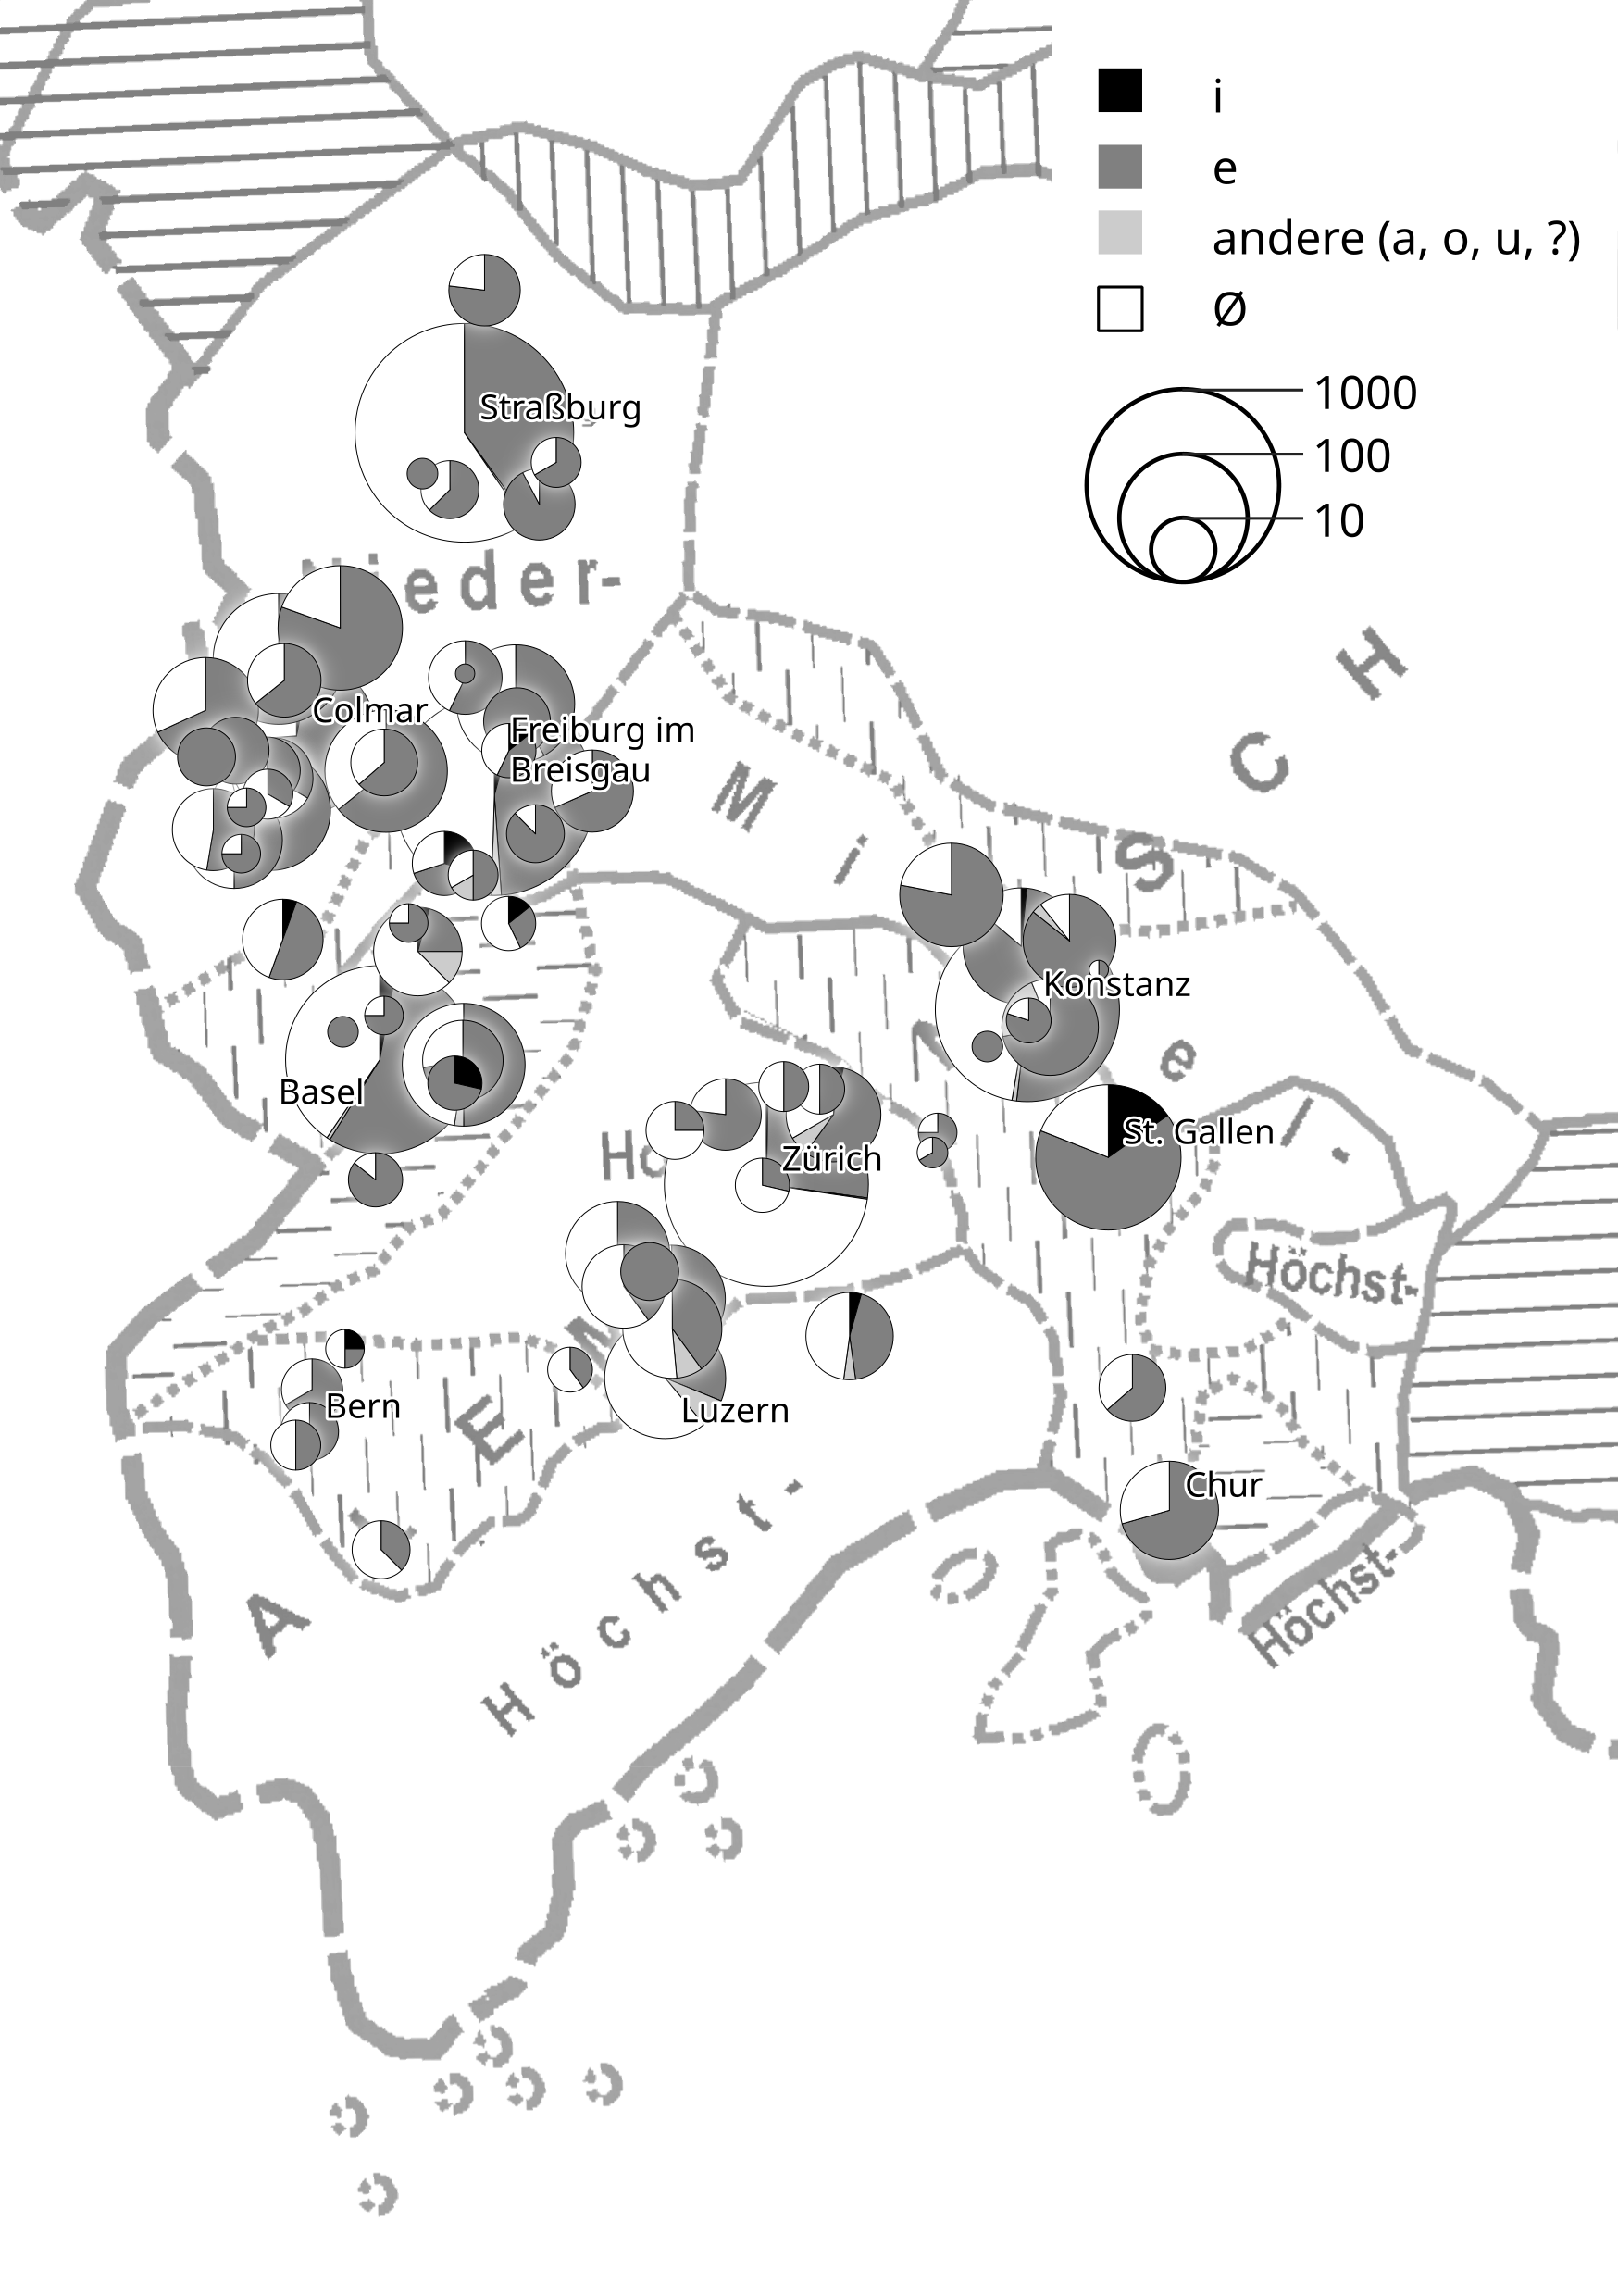
\includegraphics[
	width=\linewidth,
	height=\textheight,
	keepaspectratio
]{./figures/2023-05-19_schwa_alem.png}
\caption{Geografische Verteilung der Stichprobe zur Schwa-Grafie
	(Hintergrundkarte: \cite{wiesinger1983:rede})}
\label{fig:caoalemschwa}
\end{figure}

In der Tat machen die 28 Belege aus St.~Gallen dort immerhin 15,2\,\% der
belegten \lit{i}-Grafien aus, wie aus \tabref{tab:ispelx} hervorgeht (diese
zeigt als Ausschnitt nur diejenigen Ausstellungsorte, an denen \norm{i}-Grafien
belegt sind). Hohe absolute Werte werden auch in Freiburg i.\,Br. (55 Belege)
sowie in Basel (25) und Konstanz (21) erreicht. Gemessen an der jeweiligen
Gesamtzahl der Belege pro Ausstellungsort machen sie allerdings nur einen
kleinen Teil aus (4,2\,\%; 2,9\,\%; 2,8\,\%). An anderen Ausstellungsorten in
der Stichprobe kommen \norm{i}-Grafien nur vereinzelt vor.

\begin{sidewaystable}
\caption{Varianten der Schwa-Grafie pro Schreibort}
\begin{tabular}{
	l @{\qquad}
	r r @{\qquad}
	r r @{\qquad}
	r r @{\qquad}
	r r @{\qquad}
	r}

\lsptoprule

Ausstellungsort
	& \norm{-i} & \%
	& \norm{-e} & \%
	& -Ø & \%
	& andere & \%
	& Summe
	\\

\midrule

Basel
	& 25	& 2,9
	& 481	& 56,0
	& 348	& 40,5
	& 5		& 0,6
	& 859
	\\

Colmar
	& 10	& 3,2
	& 222	& 70,7
	& 82	& 26,1
	& 		&
	& 314
	\\

Denzlingen
	& 1 & 14,3
	& 3	& 42,9
	& 3	& 42,9
	& 	&
	& 7
	\\

Freiburg i.\,Br.
	& 55	& 4,2
	& 589	& 44,7
	& 652	& 49,5
	& 21	& 1,6
	& 1317
	\\

Guebwiller
	& 1		& 3,1
	& 15	& 46,9
	& 16	& 50,0
	& 		&
	& 32
	\\

Kl.~Einsiedeln
	& 1		& 4,3
	& 10	& 43,5
	& 11	& 47,8
	& 1		& 4,3
	& 23
	\\

Kl.~Fraubrunnen
	& 1	& 25,0
	& 1	& 25,0
	& 2	& 50,0
	&	&
	& 4
	\\

Kl.~Olsberg
	& 2	& 28,6
	& 5	& 71,4
	&	&
	&	&
	& 7
	\\

Kl.~Sitzenkirch
	& 1		& 4,2
	& 5		& 20,8
	& 15	& 62,5
	& 3		& 12,5
	& 24
	\\

Kl.~Töss
	& 1		& 3,3
	& 17	& 56,7
	& 10	& 33,3
	& 2		& 6,7
	& 30
	\\

Konstanz
	& 21 	& 2,8
	& 364	& 49,1
	& 351	& 47,3
	& 6		& 0,8
	& 742
	\\

Luzern
	& 2		& 2,6
	& 22	& 28,6
	& 47	& 61,0
	& 6		& 7,8
	& 77
	\\

Mulhouse
	& 1	& 5,6
	& 9	& 50,0
	& 8	& 44,4
	&	&
	& 18
	\\

Schönau i.\,Sw.
	& 1	& 14,3
	& 2	& 28,6
	& 4	& 57,1
	&	&
	& 7
	\\

St.~Gallen
	& 28	& 15,2
	& 121	& 65,8
	& 35	& 19,0
	&		&
	& 184
	\\

Staufen i.\,Br.
	& 3 & 30,0
	& 4	& 40,0
	& 3	& 30,0
	&	&
	& 10
	\\

Überlingen
	& 1		& 1,5	
	& 55	& 84,6
	& 9		& 13,8
	&		&
	& 65
	\\

Zürich
	& 5		& 0,3
	& 406	& 26,8
	& 1100	& 72,7
	& 3		& 0,2
	& 1514
	\\

\lspbottomrule
\end{tabular}
\label{tab:ispelx}
\end{sidewaystable}

Die Form \lit{ani} für mittelhochdeutsch \norm{āne}, althochdeutsch \norm{ānu}
\wdef{ohne}, ist ein einziges Mal in Konstanz belegt und mit ihrem Kontext in
\REF{ex:konst_ani} aufgeführt.

\begin{exe}
\ex\label{ex:konst_ani}
	\gll alſo daz ſie deſ gæltiſ gewiſſet vnde gwert werden ani giværde \\
		also dass sie des Geldes versichert und gewährt werden ohne
			Hinterhalt \\
	\trans \wdef{auf die Weise, dass sie ohne Arglist das Geld zugesichert und
		ausgezahlt bekommen}
		\parencites(Nr.~17, Konstanz, 1251)[26,22]{cao1}
\end{exe}

Auch \lit{umbi} \wdef{um}, das zur Präposition mittelhochdeutsch \norm{umbe},
althochdeutsch \norm{umbi}, gehört, tritt mit vier Belegen nur selten in der
Stichprobe auf. Es entfallen drei Belege auf Colmar, zwei davon auf Nr.~N~53
\autocites(Colmar, 1264)[37,2--17]{cao5}, und ein Beleg auf Freiburg i.\,Br.
\autocites(Nr.~2580, Freiburg i.\,Br., 1297)[9,21--33]{cao4}. Einer der Belege
aus Colmar wird in \REF{ex:col_umbi} zitiert.

\begin{exe}
\ex\label{ex:col_umbi}
	\gll daz wir {daz ſelbe} g\sscr{v}{o}t vmbi daz halbe wider enpfangen han \\
		dass wir dasselbe Gut um das halbe wieder empfangen haben \\
	\trans \wdef{dass wir dasselbe Gut für die Hälfte \textins{der Einkünfte;
		vgl.~\cite[23]{caor}} zurückempfangen haben}
		\parencites(Nr.~N~92, Colmar, 1269)[64,27--28]{cao5}
\end{exe}

Bemerkenswert ist, dass in der Freiburger Urkunde Nr.~2590
\autocites(1297)[15,32--16,4]{cao4} außer dem einen Beleg für \lit{vmbi}
\wdef{um} (15,39) an allen sechs anderen Stellen die Form \lit{vmbe} steht und
\lit{i} auch sonst nicht als Grafie für Schwa dient.

Ähnlich schwach bezeugt sind Formen des Typs \lit{frowin} zu mittelhochdeutsch
\norm{vrouwen} \wdef{Frau (\textsc{obl.sg}), Frauen}, die sich auf drei Belege
aus Colmarer und zwei Belege aus Baseler Urkunden verteilen. Wie zu erwarten, stehen
diese Belege im Dat.{\slash}Gen.~Sg. sowie im Nom.\ und Dat.~Pl., der im
Althochdeutschen\il{Althochdeutsch} in allen Fällen \norm{frouwūn} lautete. Ein
Beispiel wird in \REF{ex:col_vrouwin} gegeben. Die Form kommt allein in dieser
Urkunde noch zwei weitere Male vor, was allen Colmarer Belegen entspricht. Über
alle Ausstellungsorte in der Stichprobe hinweg endet der Nom.~Sg.\ des Lemmas
\norm{vrouwe} \wdef{(Edel-)Frau} in 64,6\,\% der Fälle auf \lit{-e}, in
31,5\,\% auf -Ø und in lediglich 3,9\,\% auf \lit{-a} (vgl.~althochdeutsch
\norm{frouwa}), jedoch nie auf \norm{-i}.

\begin{exe}
\ex\label{ex:col_vrouwin}
	\gll {da mitte} die vorgenantin frowin geirrit / vnd biſwert m\sscr{o}{e}htint
			werdin \\
		womit die vorgenannten Frau-\textsc{nom.pl.\FemF} gestört {} und
			belästigt könnten werden \\
	\trans \wdef{womit die vorgenannten Frauen gestört und belästigt werden
		könnten}
		\parencites(Nr.~3293, Colmar, 1299)[446,24]{cao4}
\end{exe}

Die Form \lit{herrin}, mittelhochdeutsch \norm{hērren} \wdef{Herrn, Herren},
die zurückgeht auf althochdeutsch \norm{hērron, -un} (Akk.~Sg.\ und im Pl.)
beziehungsweise \norm{hērrin} (Dat./Gen.~Sg.;
\cite[vgl.][289--292]{braune2023}), ist in der Stichprobe mit 43 Belegen
vertreten, nämlich in St.~Gallen (12 Belege), Basel (11), Freiburg i.\,Br. (5),
Zürich (3), Colmar (2), Konstanz und Staufen i.\,Br. (je 2) sowie in
Guebwiller, Kl.~Olsberg, Kl.~Töss und Mulhouse (je 1). Auffällig ist, dass
allein sechs Belege für St.~Gallen auf die Urkunde Nr.~628
\autocite[55,35--57,7]{cao2} entfallen, aus der in \REF{ex:stg_herrin} zitiert
wird. Daneben tritt noch je einmal \lit{herri} zu mittelhochdeutsch
\norm{hērre}, althochdeutsch \norm{hērro} \wdef{Herr}, in Colmar und Überlingen
auf, wie in \REF{ex:col_herri} gezeigt. Darüber hinaus steht in der gesamten
Stichprobe in 87,4\,\% der Fälle im Nom.~Sg.\ eine Form wie \lit{her}. Formen
wie \lit{herre} kommen mit 12,5\,\% wesentlich seltener vor, während sich die
zwei Fälle mit \lit{-i} auf lediglich 0,05\,\% belaufen. Formen wie
*\lit{herro} und *\lit{herru} sind in der Stichprobe nicht belegt.

\begin{exe}
\ex \label{ex:herrin}
	\begin{xlist}
	\ex\label{ex:stg_herrin}
		\setlength{\glossglue}{5pt plus 2pt minus 1pt}
		\gll dc denne die tohtira alle zemime herrin dim abte zeſant GAllin
				koment\\
			dass dann die Töchter alle zu=meinem Herr-\textsc{obl.sg.\MascM}
				dem Abt zu=Sankt Gallen kommen \\
		\trans \wdef{dass dann die Töchter alle zu meinem Herrn, dem Abt von
			St.~Gallen, kommen}
			\parencites(Nr.~628, St.~Gallen, 1284)[56,34]{cao2}

	\ex\label{ex:col_herri}
		\gll Do dirri brief geſcriben wart, do was vnſer herri dvſint vn̄ zwei
				hvndert vn̄ ſehzzit vn̄ vier iaric \\
			Als dieser Urkunde geschrieben wurde da war unser
				Herr-\textsc{nom.sg.\MascM} tausend und zwei hundert und
				sechzig und vier jährig \\
		\trans \wdef{Als diese Urkunde geschrieben wurde, da war unser Herr
			1.264 Jahre alt.}
			\parencites(Nr.~N~53, Colmar, 1264)[37,15]{cao5}
\end{xlist}
\end{exe}

Der größte Anteil an \lit{i}-Grafien in der Stichprobe entfällt auf Formen wie
\lit{hörint} zu mittelhochdeutsch \norm{hȫrent}, althochdeutsch
\norm{hōrėnt} \wdef{hören (\textsc{3pl.ind.prs})}. Die Belege verteilen sich
auf die Ausstellungsorte Freiburg i.\,Br. (43 Belege), Konstanz (18),
St.~Gallen (15), Basel (12), Zürich (2), Colmar, Denzlingen, Kl.~Einsiedeln,
Kl.~Fraubrunnen, Kl.~Olsberg, Kl.~Sitzenkirch, Luzern, Schönau im Schwarzwald
und Staufen i.\,Br. (je 1). Hier verteilen sich von den Belegen aus St.~Gallen
sechs auf die Urkunde Nr.~629 \autocites(St.~Gallen, 1284)[57,9--57,35]{cao2}.
Die Wortform \norm{hȫrent} kommt stereotyp in der Promulgatio, also der
Verkündigungsformel nahezu aller Urkunden im \CAO{} vor, wie in
\REF{ex:fribr_hoerint} exemplarisch angeführt.

\begin{exe}
\ex\label{ex:fribr_hoerint}
	\gll Allen die diſen brief ſehint oder h\sscr{o}{e}rint leſin den kv̓nde ich fro
			Jvnte hern C\sscr{v}{o}nrat ſchnewelins ſeligen hvſfrôwe deſ jvngen von
			Friburch \\
		Allen die diesen Urkunde sehen-\textsc{3pl.ind.prs} oder
			hören-\textsc{3pl.ind.prs} lesen denen verkünde ich Frau Junte Herrn
			Konrad Schnewelins selige Ehefrau des Jungen von Freiburg \\
	\trans \wdef{Allen, die diese Urkunde sehen oder verlesen hören, verkünde
		ich, Frau Junte, die Ehefrau Herrn Konrads des Jungen von Freiburg
		selig \textelp{}}
		\parencites(Nr.~328, Freiburg i.\,Br., 1277)[314,33--34]{cao1}
\end{exe}

Insgesamt betrachtet kommt \lit{i} in der Stichprobe zwar als Schreibweise für
einen unbetonten Nebensilbenvokal vor, liegt aber in der Häufigkeit weit hinter
Schreibweisen mit \lit{e} zurück. Auffällig ist, dass \lit{i} in der
Stichprobe passend\is{Validierung} zu \posscite[132, 136--137]{boesch1946}
Beobachtung nahezu ausschließlich in gedeckten Nebensilben auftritt, also in
unbetonter Stellung vor Konsonant: \lit{herrin}, \lit{frowin},
\lit{hörint}. Darüber hinaus zeigt gerade \lit{herrin} \wdef{Herren, Herrn} als
schwaches Maskulinum, dass \lit{i} an diesen Stellen unabhängig vom Lautwert
der entsprechenden Kasusform\is{Kasus} im Althochdeutschen\il{Althochdeutsch}
steht \autocite[vgl.][289--292]{braune2023}. Umgekehrt darf also davon
ausgegangen werden, dass Formen vom Typ \lit{beidi} \wdef{beide} nicht
typischerweise \lit{-i} für Schwa enthalten, zumal in keiner der betroffenen
Urkunden (\cite[124,18--33; 205,30--45]{cao1}; \cite[175,1--33]{cao5}; Nrn.~81,
190, N~230) regelmäßig \lit{-i} im unbetonten absoluten Auslaut steht.

\il{Alemannisch|)}
\is{Stichprobe|)}
\is{Dialektgeografie|)}
\is{Nebensilbenabschwächung|)}

%%%%%%%%%%%%%%%%%%%%%%%%%%%%%%%%%%%%%%%%%%%%%%%%%%%%%%%%%%%%%%%%%%%%%%%%%%%%%%%%

\chapter{Belegzahlen zur Adjektivstichprobe}
\label{sec:caoadjquanttab}
\is{Stichprobe|(}

Die folgende Tabelle schlüsselt die Menge der ausgewerteten Belege pro
Ausstellungsort in der Stichprobe zur Adjektivflexion in
\sectref{sec:adjdeclcao} auf.

\section{Straßburg}

\begin{tabularx}{\linewidth}{X r r r r}
\lsptoprule
Ausstellungsort
	& \makecell{Urk.\\ insges.}
	& \makecell{Urk. in\\ Stichprobe}
	& \makecell{Belege\\ insges.}
	& \makecell{Belege\\ ausgew.}
	\\
\midrule

Straßburg
	& 219
	& 122
	& 408
	& 178
	\\

Appenweier
	& 1
	& 1
	& 7
	& 3
	\\

Haguenau
	& 3
	& 3
	& 10
	& 3
	\\

Kl. Eschau
	& 1
	& 1
	& 1
	& 1
	\\

\midrule

Summe
	& 224
	& 127
	& 426
	& 185
	\\

\lspbottomrule
\end{tabularx}

%------------------------------------------------------------------------------%

\section{Basel}

\begin{tabularx}{\linewidth}{X r r r r}
\lsptoprule
Ausstellungsort
	& \makecell{Urk.\\ insges.}
	& \makecell{Urk. in\\ Stichprobe}
	& \makecell{Belege\\ insges.}
	& \makecell{Belege\\ ausgew.}
	\\
\midrule

Basel
	& 117
	& 73
	& 216
	& 75
	\\

Beuggen
	& 4
	& 3
	& 9
	& 2
	\\

Mulhouse
	& 3
	& 3
	& 7
	& 2
	\\

Rheinfelden (Kt.~Aargau)
	& 13
	& 12
	& 52
	& 14
	\\

\midrule

Summe
	& 137
	& 91
	& 284
	& 93
	\\

\lspbottomrule
\end{tabularx}

%------------------------------------------------------------------------------%

\section{Zürich}

\begin{tabularx}{\linewidth}{X r r r r}
\lsptoprule
Ausstellungsort
	& \makecell{Urk.\\ insges.}
	& \makecell{Urk. in\\ Stichprobe}
	& \makecell{Belege\\ insges.}
	& \makecell{Belege\\ ausgew.}
	\\
\midrule

Zürich
	& 143
	& 74
	& 244
	& 70
	\\

Eschenbach (Kt.~Luzern)
	& 6
	& 6
	& 34
	& 9
	\\

Hohenrain
	& 8
	& 6
	& 31
	& 15
	\\

Kl. Einsiedeln
	& 3
	& 2
	& 8
	& 3
	\\

Kl. Töss
	& 6
	& 3
	& 16
	& 4
	\\

Regensberg
	& 3
	& 3
	& 5
	& 2
	\\

\midrule

Summe
	& 169
	& 94
	& 338
	& 103
	\\

\lspbottomrule
\end{tabularx}

%------------------------------------------------------------------------------%

\section{Konstanz}

\begin{tabularx}{\linewidth}{X r r r r}
\lsptoprule
Ausstellungsort
	& \makecell{Urk.\\ insges.}
	& \makecell{Urk. in\\ Stichprobe}
	& \makecell{Belege\\ insges.}
	& \makecell{Belege\\ ausgew.}
	\\
\midrule

Konstanz
	& 46
	& 36
	& 202
	& 55
	\\

Kl. Kreuzlingen
	& 1
	& 1
	& 6
	& 2
	\\

Kl. Münsterlingen
	& 4
	& 1
	& 14
	& 4
	\\

Kl. Salem
	& 5
	& 5
	& 13
	& 4
	\\

Nellenburg
	& 2
	& 2
	& 24
	& 7
	\\

Schloss Altenklingen
	& 1
	& 1
	& 2
	& 1
	\\

St. Gallen
	& 16
	& 15
	& 68
	& 22
	\\

Tannegg
	& 1
	& 1
	& 9
	& 2
	\\

Überlingen
	& 14
	& 9
	& 27
	& 10
	\\

\midrule

Summe
	& 92
	& 73
	& 370
	& 107
	\\

\lspbottomrule
\end{tabularx}

%------------------------------------------------------------------------------%

\section{Ulm}

\begin{tabularx}{\linewidth}{X r r r r}
\lsptoprule
Ausstellungsort
	& \makecell{Urk.\\ insges.}
	& \makecell{Urk. in\\ Stichprobe}
	& \makecell{Belege\\ insges.}
	& \makecell{Belege\\ ausgew.}
	\\
\midrule

Ulm
	& 16
	& 15
	& 64
	& 34
	\\

Kl. Blaubeuren
	& 1
	& 1
	& 9
	& 6
	\\

Kl. Herbrechtingen
	& 1
	& 1
	& 8
	& 5
	\\

\midrule

Summe
	& 18
	& 17
	& 81
	& 45
	\\

\lspbottomrule
\end{tabularx}

%------------------------------------------------------------------------------%

\section{Augsburg}

\begin{tabularx}{\linewidth}{X r r r r}
\lsptoprule
Ausstellungsort
	& \makecell{Urk.\\ insges.}
	& \makecell{Urk. in\\ Stichprobe}
	& \makecell{Belege\\ insges.}
	& \makecell{Belege\\ ausgew.}
	\\
\midrule

Augsburg
	& 95
	& 78
	& 517
	& 141
	\\

Adelzhausen
	& 1
	& 1
	& 6
	& 2
	\\

Aichach
	& 4
	& 3
	& 34
	& 14
	\\

Bocksberg (Laugna)
	& 1
	& 1
	& 13
	& 5
	\\

Kl. Holzen
	& 2
	& 2
	& 8
	& 4
	\\

Kl. Oberschönenfeld
	& 5
	& 5
	& 14
	& 2
	\\

Kl. Weihenberg
	& 1
	& 1
	& 1
	& 1
	\\

\midrule

Summe
	& 109
	& 91
	& 593
	& 169
	\\

\lspbottomrule
\end{tabularx}

%------------------------------------------------------------------------------%

\section{Nürnberg}

\begin{tabularx}{\linewidth}{X r r r r}
\lsptoprule
Ausstellungsort
	& \makecell{Urk.\\ insges.}
	& \makecell{Urk. in\\ Stichprobe}
	& \makecell{Belege\\ insges.}
	& \makecell{Belege\\ ausgew.}
	\\
\midrule

Nürnberg
	& 26
	& 18
	& 76
	& 39
	\\

Kl. Seligenporten
	& 3
	& 3
	& 44
	& 20
	\\

\midrule

Summe
	& 29
	& 21
	& 120
	& 59
	\\

\lspbottomrule
\end{tabularx}

%------------------------------------------------------------------------------%

\section{Regensburg}

\begin{tabularx}{\linewidth}{X r r r r}
\lsptoprule
Ausstellungsort
	& \makecell{Urk.\\ insges.}
	& \makecell{Urk. in\\ Stichprobe}
	& \makecell{Belege\\ insges.}
	& \makecell{Belege\\ ausgew.}
	\\
\midrule

Regensburg
	& 53
	& 43
	& 245
	& 88
	\\

Abensberg
	& 1
	& 1
	& 4
	& 2
	\\

Kl. Pettendorf
	& 5
	& 3
	& 17
	& 6
	\\

Kl. Pielenhofen
	& 5
	& 4
	& 16
	& 6
	\\

Laaber
	& 1
	& 1
	& 5
	& 3
	\\

\midrule

Summe
	& 65
	& 52
	& 287
	& 105
	\\

\lspbottomrule
\end{tabularx}

%------------------------------------------------------------------------------%

\section{München}

\begin{tabularx}{\linewidth}{X r r r r}
\lsptoprule
Ausstellungsort
	& \makecell{Urk.\\ insges.}
	& \makecell{Urk. in\\ Stichprobe}
	& \makecell{Belege\\ insges.}
	& \makecell{Belege\\ ausgew.}
	\\
\midrule

München
	& 22
	& 19
	& 94
	& 54
	\\

Kl. Indersdorf
	& 2
	& 2
	& 13
	& 6
	\\

Sachsenhausen (Egling)
	& 1
	& 1
	& 13
	& 6
	\\

\midrule

Summe
	& 25
	& 20
	& 120
	& 66
	\\

\lspbottomrule
\end{tabularx}

%------------------------------------------------------------------------------%

\section{Salzburg}

\begin{tabularx}{\linewidth}{X r r r r}
\lsptoprule
Ausstellungsort
	& \makecell{Urk.\\ insges.}
	& \makecell{Urk. in\\ Stichprobe}
	& \makecell{Belege\\ insges.}
	& \makecell{Belege\\ ausgew.}
	\\
\midrule

Salzburg
	& 75
	& 59
	& 309
	& 88
	\\

Burgstall Kalham
	& 1
	& 1
	& 4
	& 1
	\\

Kl. Berchtesgaden
	& 2
	& 1
	& 12
	& 3
	\\

Kl. Höglwörth
	& 1
	& 1
	& 2
	& 2
	\\

Kl. Michaelbeuern
	& 1
	& 1
	& 14
	& 3
	\\

Mattsee
	& 1
	& 1
	& 6
	& 2
	\\

Reichenhall
	& 2
	& 1
	& 2
	& 1
	\\

Schloss Staufeneck
	& 2
	& 2
	& 9
	& 2
	\\

\midrule

Summe
	& 85
	& 67
	& 358
	& 102
	\\

\lspbottomrule
\end{tabularx}

%------------------------------------------------------------------------------%

\section{Wien}

\begin{tabularx}{\linewidth}{X r r r r}
\lsptoprule
Ausstellungsort
	& \makecell{Urk.\\ insges.}
	& \makecell{Urk. in\\ Stichprobe}
	& \makecell{Belege\\ insges.}
	& \makecell{Belege\\ ausgew.}
	\\
\midrule

Wien
	& 51
	& 45
	& 197
	& 60
	\\

Kaiserebersdorf
	& 4
	& 2
	& 14
	& 6
	\\

Klosterneuburg
	& 9
	& 8
	& 45
	& 14
	\\

Stift Heiligenkreuz
	& 8
	& 8
	& 40
	& 12
	\\

\midrule

Summe
	& 71
	& 58
	& 296
	& 92
	\\

\lspbottomrule
\end{tabularx}

\is{Stichprobe|)}

%%%%%%%%%%%%%%%%%%%%%%%%%%%%%%%%%%%%%%%%%%%%%%%%%%%%%%%%%%%%%%%%%%%%%%%%%%%%%%%%

\chapter{Verzeichnis der zitierten Handschriften}
\label{ch:hssverz}

Die folgenden Handschriftensignaturen werden im Text genannt. Weiterführende
Informationen zur jeweiligen Handschrift sowie Links zu
Digitalisaten\is{Digitalisat} können dem \tit{Handschriftencensus} (\tit{HSC};
\nosh\cite{hsc}) unter der angegebenen ID entnommen werden, zum Beispiel
\url{https://handschriftencensus.de/2776} für Basel, Universitätsbibl.,
Cod.~B~VIII~27. Da nicht alle Handschriften den Sammlungskriterien des
\tit{HSC} entsprechen, existiert dort nicht zu jeder genannten Sig\-natur ein
Eintrag.\\

\noindent
\begin{tabularx}{\linewidth}{@{} >{\raggedright\arraybackslash}X l @{}}
Basel, Universitätsbibliothek, Cod. B VIII 27
	& \autocite[2776]{hsc} \\
Basel, Universitätsbibliothek, Cod. N I 3, Nr. 89
	& \autocite[1158]{hsc} \\
Bern, Staatsarchiv, StABE C I a, Stift 1293.11.30
	& ---%
	\footnote{Vgl.~\url{https://www.query.sta.be.ch/detail.aspx?ID=62091}.} % 08.01.24
	\\
Dresden, Sächsische Landesbibliothek, Mscr.Dresd.M.32
	& \autocite[7549]{hsc} \\
Gießen, Universitätsbibliothek, Hs 97
	& \autocite[1102]{hsc} \\
Heidelberg, Universitätsbibliothek, Cod. Pal. germ. 361
	& \autocite[1181]{hsc} \\
Heidelberg, Universitätsbibliothek, Cod. Pal. germ. 848
	& \autocite[4957]{hsc} \\
Karlsruhe, Badische Landesbibliothek, Cod. Aug. 52
	& \autocite[8470]{hsc} \\
Köln, Historisches Archiv der Stadt, Best. 210, U~3/759
	& ---%
	\footnote{Digitalisat:~\href{%
		https://historischesarchivkoeln.de/document/Vz_E9493491-3A61-4625-8DB0-09465C24BCC8% 08.01.24
	}{%
		https://historischesarchivkoeln.de/document/Vz\_E949\allowbreak{}%
		3491-3A61-4625-8DB0-0946\allowbreak{}5C24\allowbreak{}BCC8}.%
	}\\
Leutkirch, Fürstliche Waldburg zu Zeil und Trauch\-burg\-sches
	Gesamt\-archiv, ZAMs 30
	& \autocite[8471]{hsc} \\
München, Bayerische Staatsbibliothek, Cgm 25
	& \autocite[8827]{hsc} \\
München, Bayerische Staatsbibliothek, Cgm 37
	& \autocite[2119]{hsc} \\
München, Bayerische Staatsbibliothek, Cgm 44
	& \autocite[1307]{hsc} \\
München, Bayerische Staatsbibliothek, Cgm 51
	& \autocite[1286]{hsc} \\
München, Bayerische Staatsbibliothek, Cgm 183
	& \autocite[9715]{hsc} \\
München, Bayerische Staatsbibliothek, Cgm 965
	& \autocite[8472]{hsc} \\
München, Bayerische Staatsbibliothek, Cgm 6247
	& \autocite[1450]{hsc} \\
München, Bayerische Staatsbibliothek, Clm 16083
	& \autocite[19293]{hsc} \\
\end{tabularx}

\noindent
\begin{tabularx}{\linewidth}{@{} >{\raggedright\arraybackslash}X l @{}}
Nordhausen, Stadtarchiv, Ms. II, Na 6
	& \autocite[1379]{hsc} \\
Nürnberg, Germanisches Nationalmuseum, Hs. 22067
	& \autocite[1189]{hsc} \\
Oxford, Bodleian Library, Cod. Junius 11
	& ---%
	\footnote{Digitalisat:~\url{https://digital.bodleian.ox.ac.uk/objects/d5e3a9fc-abaa-4649-ae48-be207ce8da15/}.} % 08.01.24
	\\
Reykjavík, Stofnun Árna Magnússonar, GKS~2365~4to
	& ---%
	\footnote{Digitalisat:~\url{https://handrit.is/manuscript/view/is/GKS04-2365/31}.} % 08.01.24
	\\
St.~Gallen, Stiftsbibliothek, Cod.~Sang.~857
	& \autocite[1211]{hsc} \\
Straßburg, Bibliothèque nationale et universitaire, ms.~2215
	& \autocite[1828]{hsc} \\
Prag, Národní knihovna České republiky, Cod.~XIII~G~43
	& \autocite[1168]{hsc} \\
Uppsala, Universitetsbibliotek, MS~DG~1
	& ---%
	\footnote{Digitalisat:~\url{http://www.alvin-portal.org/alvin/view.jsf?pid=alvin-record:60279}.} % 08.01.24
	\\
Vorau, Archiv des Augustiner-Chorherrenstifts, Ms~276
	& \autocite[1432]{hsc} \\
Wien, Österreichische Nationalbibliothek, Cod.~2685
	& \autocite[2013]{hsc} \\
Wien, Österreichische Nationalbibliothek, Cod.~2687
	& \autocite[6494]{hsc} \\
Wien, Österreichische Nationalbibliothek, Cod.~2693
	& \autocite[1215]{hsc} \\
Wien, Österreichische Nationalbibliothek, Cod.~2779
	& \autocite[2693]{hsc} \\
Wien, Österreichische Nationalbibliothek, Cod.~12487
	& \autocite[3394]{hsc} \\
Wolfenbüttel, Herzog August Bibliothek, Cod.~Guelf.~3.1~Aug.~2º
	& \autocite[8396]{hsc} \\
Wolfenbüttel, Herzog August Bibliothek, Cod.~Guelf.~15.2~Aug.~2º
	& \autocite[6668]{hsc} \\
\end{tabularx}


%%%%%%%%%%%%%%%%%%%%%%%%%%%%%%%%%%%%%%%%%%%%%%%%%%%
%%             Backmatter                       %%%
%%%%%%%%%%%%%%%%%%%%%%%%%%%%%%%%%%%%%%%%%%%%%%%%%%%

% \issa{some term with pages}{some other term also of interest}
% \is{some term| see {some other term}}
\ilsa{Mitteldeutsch}{Ost-, Westmitteldeutsch}
\ilsa{Oberdeutsch}{Nord-, Ost-, Westoberdeutsch}
\ilsa{Ostmitteldeutsch}{Böhmisch, Thüringisch}
\ilsa{Westmitteldeutsch}{Hessisch, \mbox{Rhein-,} Mittel\-fränkisch}
\ilsa{Westoberdeutsch}{Alemannisch, Schwäbisch}
\il{Bosnisch| see {BKMS}}
\il{Deutsch| see{Neuhochdeutsch}}
\il{Hebräisch| see {Ivrit}}
\il{Kroatisch| see {BKMS}}
\il{Mazedonisch| see {BKMS}}
\il{Nordoberdeutsch| see {Ostfränkisch}}
\il{Ostoberdeutsch| see {Bairisch}}
\il{Serbisch| see {BKMS}}
% \issa{Animata}{Belebtheit}
% \issa{Belebtheit}{Animata; Inanimata}
% \issa{Concord}{Kongruenz, formale}
% \issa{Distanzstellung}{Mittelfeld}
% \issa{Distanz}{Domäne}
% \issa{Domäne}{Distanz, syntaktische}
% \issa{Inanimata}{Belebtheit}
% \issa{Index}{Kongruenz, semantische}
% \issa{Kongruenz}{Concord; Index}
% \issa{Mittelfeld}{Distanzstellung}
\is{Geschlecht!soziales| see {Gender}}
\is{Geschlecht!grammatisches| see {Genus}}

% % There is normally no need to change the backmatter section
\backmatter
\phantomsection%this allows hyperlink in ToC to work
{\sloppy\printbibliography[heading=references]}
\cleardoublepage

\phantomsection
\addcontentsline{toc}{chapter}{\lsIndexTitle}
\addcontentsline{toc}{section}{\lsNameIndexTitle}
\ohead{\lsNameIndexTitle}
\printindex
\cleardoublepage

% \phantomsection
% \addcontentsline{toc}{section}{\lsLanguageIndexTitle}
% \ohead{\lsLanguageIndexTitle}
% \printindex[lan]
% \cleardoublepage
%
% \phantomsection
% \addcontentsline{toc}{section}{\lsSubjectIndexTitle}
% \ohead{\lsSubjectIndexTitle}
% \printindex[sbj]
% \ohead{}

\end{document}
% you can create your book by running
% xelatex main.tex
